\documentclass{styles/mimosis}

% ============================================
% Medical & Healthcare
% ============================================
\newacronym{mimic}{MIMIC}{Medical Information Mart for Intensive Care}
\newacronym{ehr}{EHR}{electronic health record}
\newacronym{icd}{ICD}{International Classification of Diseases}
\newacronym{umls}{UMLS}{Unified Medical Language System}
\newacronym{snomed}{SNOMED}{Systematized Nomenclature of Medicine}

% ============================================
% Privacy & Regulation
% ============================================
\newacronym{gdpr}{GDPR}{General Data Protection Regulation}
\newacronym{hipaa}{HIPAA}{Health Insurance Portability and Accountability Act}
\newacronym{pii}{PII}{personally identifiable information}
\newacronym{dp}{DP}{differential privacy}

% ============================================
% NLP & Machine Learning - General
% ============================================
\newacronym{nlp}{NLP}{natural language processing}
\newacronym{llm}{LLM}{large language model}
\newacronym{ai}{AI}{artificial intelligence}
\newacronym{ner}{NER}{named entity recognition}
\newacronym{qa}{QA}{question answering}
\newacronym{icl}{ICL}{in-context learning}
\newacronym{api}{API}{application programming interface}

% ============================================
% Neural Network Architectures
% ============================================
\newacronym{gpt}{GPT}{Generative Pre-trained Transformer}
\newacronym{bert}{BERT}{Bidirectional Encoder Representations from Transformers}
\newacronym{lstm}{LSTM}{Long Short-Term Memory}

% ============================================
% Training & Fine-tuning Methods
% ============================================
\newacronym{sft}{SFT}{supervised fine-tuning}
\newacronym{rl}{RL}{reinforcement learning}
\newacronym{rlhf}{RLHF}{Reinforcement Learning from Human Feedback}
\newacronym{rlaif}{RLAIF}{Reinforcement Learning from AI Feedback}

% ============================================
% Preference Optimization Methods
% ============================================
\newacronym{dpo}{DPO}{Direct Preference Optimization}
\newacronym{kto}{KTO}{Kahneman-Tversky Optimization}
\newacronym{orpo}{ORPO}{Odds Ratio Preference Optimization}
\newacronym{simpo}{SimPO}{Simple Preference Optimization}
\newacronym{xpo}{XPO}{Exploratory Preference Optimization}
\newacronym{scir}{SCIR}{Self-Consistent Internal Reward}

% ============================================
% Evaluation Metrics
% ============================================
\newacronym{rouge}{ROUGE}{Recall-Oriented Understudy for Gisting Evaluation}
\newacronym{bleu}{BLEU}{Bilingual Evaluation Understudy}
\newacronym{mauve}{MAUVE}{Measuring Automatic eValuation of text Using Embeddings}
\newacronym{fid}{FID}{Fréchet Inception Distance}

% ============================================
% Annotation & Tagging
% ============================================
\newacronym{iob}{IOB}{Inside-Outside-Beginning}

% ============================================
% Additional Medical
% ============================================
\newacronym{icu}{ICU}{Intensive Care Unit}
\newacronym{phi}{PHI}{Protected Health Information}

% ============================================
% Additional ML/NLP Methods
% ============================================
\newacronym{rag}{RAG}{Retrieval-Augmented Generation}
\newacronym{lora}{LoRA}{Low-Rank Adaptation}
\newacronym{crf}{CRF}{Conditional Random Field}
\newacronym{cot}{CoT}{Chain of Thought}
\newacronym{re}{RE}{relation extraction}
\newacronym{tfidf}{TF-IDF}{Term Frequency-Inverse Document Frequency}
\newacronym{lm}{LM}{language model}

% ============================================
% Institutions
% ============================================
\newacronym{aphp}{AP-HP}{Assistance Publique -- Hôpitaux de Paris}


\usepackage{metalogo}

%%%%%%%%%%%%%%%%%%%%%%%%%%%%%%%%%%%%%%%%%%%%%%%%%%%%%%%%%%%%%%%%%%%%%%%%
% Some of my favourite personal adjustments
%%%%%%%%%%%%%%%%%%%%%%%%%%%%%%%%%%%%%%%%%%%%%%%%%%%%%%%%%%%%%%%%%%%%%%%%
%
% These are the adjustments that I consider necessary for typesetting
% a nice thesis. However, they are *not* included in the template, as
% I do not want to force you to use them.

% This ensures that I am able to typeset bold font in table while still aligning the numbers
% correctly.
\usepackage{etoolbox}

\usepackage{siunitx}
\usepackage{lscape}
\DeclareSIUnit\px{px}

\sisetup{%
  detect-all           = true,
  detect-family        = true,
  detect-mode          = true,
  detect-shape         = true,
  detect-weight        = true,
}

%%%%%%%%%%%%%%%%%%%%%%%%%%%%%%%%%%%%%%%%%%%%%%%%%%%%%%%%%%%%%%%%%%%%%%%%
% Hyperlinks & bookmarks
%%%%%%%%%%%%%%%%%%%%%%%%%%%%%%%%%%%%%%%%%%%%%%%%%%%%%%%%%%%%%%%%%%%%%%%%

\usepackage[%
  unicode,
  colorlinks = true,
  citecolor  = RoyalBlue,
  linkcolor  = RoyalBlue,
  urlcolor   = RoyalBlue,
  unicode,
  ]{hyperref}
\hypersetup{
  pdftitle=Synthetic Data Generation for Clinical Natural Language Processing,
  pdfauthor=Simon Meoni
}

\usepackage{bookmark}


%%%%%%%%%%%%%%%%%%%%%%%%%%%%%%%%%%%%%%%%%%%%%%%%%%%%%%%%%%%%%%%%%%%%%%%%
% Fonts
%%%%%%%%%%%%%%%%%%%%%%%%%%%%%%%%%%%%%%%%%%%%%%%%%%%%%%%%%%%%%%%%%%%%%%%%

\ifxetexorluatex
  \setmainfont[Ligatures=TeX]{TeX Gyre Pagella} % Palatino clone
  \linespread{1.05} % a bit more for Palatino
  \RequirePackage{unicode-math}
  \setmathfont{TeX Gyre Pagella Math}
\else
  \usepackage[lf]{ebgaramond}
  \usepackage[oldstyle,scale=0.7]{sourcecodepro}
  \singlespacing
\fi

\usepackage{minitoc}
\usepackage[ruled,vlined,boxed]{algorithm2e}
\usepackage{enumitem}
\usepackage{microtype}
\usepackage{latexsym}
\usepackage{adjustbox}
\usepackage{booktabs}
\usepackage{multirow}
\usepackage{fancyvrb}
\usepackage{xcolor}
\usepackage{subcaption}
\usepackage{amsmath,amssymb,amsfonts}
\usepackage{algorithmic}
\usepackage{graphicx}
\usepackage{textcomp}
\usepackage{bm}
\usepackage{xspace}
\usepackage{fancyvrb}
\usepackage{fvextra}
\usepackage{tcolorbox}

\makeindex
\makeglossaries

%%%%%%%%%%%%%%%%%%%%%%%%%%%%%%%%%%%%%%%%%%%%%%%%%%%%%%%%%%%%%%%%%%%%%%%%
% Custom Commands and Environments
%%%%%%%%%%%%%%%%%%%%%%%%%%%%%%%%%%%%%%%%%%%%%%%%%%%%%%%%%%%%%%%%%%%%%%%%
%%%%%%%%%%%%%%%%%%%%%%%%%%%%%%%%%%%%%%%%%%%%%%%%%%%%%%%%%%%%%%%%%%%%%%%%
% Custom Commands and Environments
%%%%%%%%%%%%%%%%%%%%%%%%%%%%%%%%%%%%%%%%%%%%%%%%%%%%%%%%%%%%%%%%%%%%%%%%

%\usepackage{fontawesome}
\usepackage{arydshln}
\usepackage{fontawesome5}
\usepackage{tikz}
\usetikzlibrary{positioning}

\usepackage{stackengine}
\def\ucr{\scalebox{1}{\stackinset{c}{}{c}{-.1pt}{%
  \textcolor{white}{\sffamily\bfseries\small ?}}{%
  \rotatebox{45}{$\blacksquare$}}}}


%%%%%%%%%%%%%%%%%%%%%%%%%%%%%%%%%%%%%%%%%%%%%%%%%%%%%%%%%%%%%%%%%%%%%%%%
% Incipit
%%%%%%%%%%%%%%%%%%%%%%%%%%%%%%%%%%%%%%%%%%%%%%%%%%%%%%%%%%%%%%%%%%%%%%%%

\title{On Modern NLP for Extraterrestrial Languages and Scripts}
\author{Simon Meoni}

\begin{document}
\glsunsetall

\frontmatter
\selectlanguage{french}

\begin{titlepage}

	\begin{center}
		\begin{minipage}[t]{0.4\textwidth}
			
\includegraphics[height=2cm]{static/media/sorbonne}
		\end{minipage}%
		\hfill
		\begin{minipage}[t]{0.4\textwidth}
			\hfill
			
\includegraphics[height=2cm]{static/media/inria}
		\end{minipage}

		\vspace{0.2cm}
		\LARGE \textsc{Université Sorbonne Université}\\
		\vspace{0.2cm}
		\normalsize \textsc{Ecole Doctorale Informatique, Télécommunications et Electronique} - ED130\\
		\vspace{0.2cm}
		\textsc{Inria de Paris / Équipe ALMAnaCH / Arkhn}\\

		\vspace{0.4cm}
		\Large \textsc{Thèse de doctorat}\\
		\normalsize Discipline : Informatique\\
		\vspace{0.4cm}
		\normalsize Présentée par \\
		\LARGE \textbf{Simon \textsc{Meoni}}\\
		\vspace{0.4cm}
		\normalsize Dirigée par \\
		\Large \textbf{Laurent \textsc{Romary}}, \textbf{Éric \textsc{De la Clergerie}} et \textbf{Théo \textsc{Ryffel}}\\
		\vspace{0.4cm}
		\normalsize Pour obtenir le grade universitaire de\\
		\Large \textsc{Docteur} de l'\textsc{Université Sorbonne Université}

		\hrulefill\\[0.2cm]

		{\Large  \textbf{Synthetic Data Generation for Clinical Natural Language Processing}}\\[0.1cm]

		\hrulefill\\

		\vspace{0.cm}
		\normalsize Présentée et soutenue publiquement le 15 Juin 2026 devant le jury composé de :\\
		\vspace{0.2cm}
		\begin{tabular*}{0.95\linewidth}{@{\extracolsep{\fill}}l l l@{}}
			Natalia \textsc{Grabar} & CNRS, STL, Université de Lille & Rapporteure \\
			Pierre \textsc{Zweigenbaum} & LISN, CNRS, Université Paris-Saclay & Rapporteur \\
			Mathieu \textsc{Constant} & ATILF, Université de Lorraine & Examinateur \\
			Lina Fatima \textsc{Soualmia} & LITIS, Université de Rouen Normandie & Examinatrice \\
			Xavier \textsc{Tannier} & LIMICS, Sorbonne Université & Examinateur \\
			% Christopher \textsc{Columbus} & Kingdom of Castile & Invited member\\
			% Margaret \textsc{Hamilton} & University of Michigan & Rapporteur \\
			% Emmy \textsc{Noether} & Georg-August-Universität Göttingen & Examinateur \\
			% Jürgen \textsc{Schmidhuber} & IDSIA & Directeur\\
			% Jean \textsc{LeCun} & Facebook AI & Co-directeur\\
			% Claude \textsc{Shannon} & MIT & Examinateur \\
			% Alan \textsc{Turing} & Princeton University & Rapporteur \\
		\end{tabular*}
	\end{center}

\end{titlepage}

\selectlanguage{english}

\newpage
\null
\thispagestyle{empty}
\newpage

\begin{center}
  \textsc{Abstract}
\end{center}
%
\noindent
%
Clinical natural language processing relies on large volumes of annotated text, yet access to real patient records remains severely restricted by privacy regulations such as GDPR and HIPAA.
This thesis investigates synthetic data generation as a privacy-preserving alternative for training clinical NLP systems.

We propose a facsimile generation approach in which synthetic clinical documents are produced by a large language model guided solely by medical concept keywords extracted from real records via UMLS, ensuring that no patient text crosses the privacy boundary.
The generator is iteratively refined through Direct Preference Optimisation (DPO) using a private contrastive scorer that compares synthetic and real documents, returning only numerical scores to the generation side.
Evaluated on MIMIC-III discharge summaries, synthetic data achieves ICD-9 classification performance comparable to or exceeding that of real data, particularly on complex label spaces where oversampling compensates for the quality gap.
We further demonstrate the generalisability of the approach to French clinical reports from AP-HP, where DPO alignment yields substantial gains in ICD-10 coding performance, confirming the language-agnostic nature of the methodology.

In parallel, we explore LLM-based weak annotation as a complementary strategy for low-resource clinical NER.
Through knowledge distillation from a large language model into smaller encoder models on the multilingual E3C corpus, we show that hybrid supervision combining LLM-generated and dictionary-based annotations achieves the best performance across five European languages, with particular benefits for low-resource settings.

Finally, we conduct a thorough privacy analysis revealing that DPO alignment, while improving generation quality, amplifies re-identification risk.
We propose keyword perturbation as a mitigation strategy that substantially reduces linkage attack success at negligible utility cost for conversational tasks.
However, discrimination attacks remain partially effective even after mitigation, underscoring that no zero-risk solution exists.

This work demonstrates that keyword-guided synthetic generation with iterative alignment offers a viable path toward privacy-preserving clinical NLP, while honestly acknowledging the residual risks and the fundamental tension between data utility and patient privacy.

\chapter*{Declaration on the Use of Artificial Intelligence}
\addcontentsline{toc}{chapter}{Declaration on the Use of Artificial Intelligence}

This thesis was prepared with the assistance of generative artificial intelligence tools.
In accordance with principles of academic integrity and transparency, I declare the following uses:

\paragraph{Writing Assistance.}
Claude (Anthropic, versions Claude 3.5 Sonnet and Claude Opus 4.5) was used via Claude Code to assist with:
\begin{itemize}
    \item Improving grammar, spelling, and fluency of drafted text
    \item Restructuring and reformulating passages for clarity
    \item LaTeX formatting and compilation error resolution
    \item Literature search suggestions and bibliography management
\end{itemize}

\paragraph{Code Development.}
Claude was used to assist with:
\begin{itemize}
    \item Debugging and refactoring Python code for experiments
    \item Writing utility scripts for data processing
\end{itemize}

\paragraph{Statement of Responsibility.}
All scientific ideas, research design, experimental methodology, data analysis, interpretation of results, and conclusions presented in this thesis are entirely my own work.
AI-generated suggestions were critically reviewed, edited, and validated before inclusion.
I take full responsibility for the content of this thesis, including any errors or omissions.

\vspace{1cm}
\noindent
\textit{No AI tools were used to generate research data, fabricate results, or produce content presented as original scientific contribution.}

\vspace{1cm}
\noindent
\textbf{Technical Details.}
The complete configuration of the AI-assisted workflow, including custom skills and project instructions, is documented in Appendix~\ref{appendix:ai_usage} and available in the thesis repository:

\begin{center}
\url{https://github.com/simonmeoni/thesis}
\end{center}

\dominitoc
\tableofcontents
\listoffigures
\listoftables
\listofalgorithms

\glsaddall
\printglossary[type=\acronymtype]

\mainmatter
\chapter{Introduction}

\section{Context: Natural Language Processing for Medical Documents}

The past two decades have witnessed a profound transformation in healthcare documentation, driven by the widespread adoption of Electronic Health Records (EHRs). These digital repositories now serve as the primary medium for capturing patient information, encompassing diagnoses, medications, treatment plans, laboratory results, imaging reports, and clinical narratives~\citep{shickel2018deep, wu2020deep}. The volume of healthcare data has grown at an unprecedented rate, with projections indicating that medical knowledge doubles approximately every 73 days~\citep{densen2011challenges}. This exponential growth presents both opportunities and challenges for healthcare systems seeking to leverage their data assets for improved patient care and clinical research.

A critical characteristic of EHR data is its heterogeneous nature, comprising both structured elements—such as coded diagnoses, vital signs, and laboratory values—and unstructured free-text narratives written by healthcare providers. Research consistently indicates that approximately 80\% of clinical data exists in unstructured format~\citep{kong2019managing, wu2022neural}, including physician notes, discharge summaries, radiology reports, and nursing assessments. This free-text component captures nuanced clinical information that structured data fields cannot adequately represent: the subtleties of symptom presentation, the reasoning behind clinical decisions, social determinants of health, and the evolution of patient conditions over time~\citep{wang2018clinical, dalianis2018clinical}.

The richness of clinical narratives makes them invaluable for understanding patient trajectories, yet their unstructured nature renders them largely inaccessible to traditional computational analysis. As~\citet{yang2022large} note, clinical notes provide a ``glimpse into the physician's brain,'' documenting not only what was observed but also the clinical reasoning process. However, without appropriate processing tools, this wealth of information remains effectively locked away, unable to contribute to secondary uses such as clinical decision support, quality improvement initiatives, or biomedical research~\citep{wu2022neural, yadav2018mining}.

Natural Language Processing (NLP) has emerged as the key technology for unlocking the potential of clinical text~\citep{wang2018clinical, yadav2018mining}. By enabling computational systems to parse, interpret, and extract meaningful information from human language, NLP bridges the gap between the expressiveness of clinical narratives and the structured data requirements of downstream applications. The field has undergone a remarkable evolution, progressing from early rule-based systems relying on handcrafted patterns and medical vocabularies to sophisticated machine learning approaches, and more recently to transformer-based language models that have achieved unprecedented performance on a wide range of clinical NLP tasks~\citep{kalyan2022ammu, wu2022neural}.

Clinical NLP encompasses a diverse array of tasks that collectively enable the transformation of free text into actionable knowledge. Traditional information extraction tasks include Named Entity Recognition (NER), which identifies and categorizes clinically relevant mentions—diseases, medications, procedures, anatomical sites—within running text~\citep{wang2019clinical, nasar2021named}. Relation Extraction determines the semantic connections between identified entities, such as linking a drug to its dosage or a symptom to its anatomical location~\citep{luo2023systematic}. Temporal reasoning situates clinical events within a timeline, enabling the reconstruction of patient histories~\citep{bethard2017semeval}. Assertion detection and negation handling distinguish between conditions that are present, absent, hypothetical, or attributed to family members~\citep{chapman2013extending}. Text classification supports tasks ranging from document triage to phenotype identification~\citep{yim2016natural}. Together, these capabilities form the foundation for applications such as automated coding, pharmacovigilance, and cohort identification for clinical trials~\citep{kreimeyer2017natural, wang2018clinical}.

The methodological landscape of clinical NLP has evolved through several distinct paradigms. Early systems relied on rule-based approaches, leveraging handcrafted patterns, regular expressions, and medical ontologies such as UMLS and SNOMED-CT to identify clinical concepts~\citep{friedman2004natural}. While interpretable and precise for well-defined patterns, these systems required extensive manual engineering and struggled with the variability inherent in clinical language. The introduction of machine learning brought statistical methods---including Conditional Random Fields (CRFs) and Support Vector Machines---that could learn patterns from annotated corpora, improving robustness to linguistic variation~\citep{jiang2011systematic}. The deep learning revolution, beginning around 2015, saw recurrent neural networks and LSTM-CRF architectures achieve state-of-the-art performance on sequence labeling tasks by learning distributed representations of clinical text~\citep{wu2018deep, si2019enhancing}. However, the most transformative shift came with the introduction of transformer-based pre-trained language models. BERT~\citep{devlin2019bert} and its biomedical and clinical variants---BioBERT~\citep{lee2020biobert}, ClinicalBERT~\citep{huang2019clinicalbert}, and PubMedBERT~\citep{gu2021domain}---demonstrated that self-supervised pre-training on large corpora yields rich contextual representations that transfer effectively to downstream tasks with minimal task-specific data. Scaling these approaches, GatorTron trained on over 90 billion words of text established that larger models and more diverse clinical training data yield consistent improvements across benchmarks~\citep{yang2022large}.

The emergence of Large Language Models (LLMs) has fundamentally expanded the scope of clinical NLP beyond traditional information extraction toward natural language generation and complex reasoning tasks~\citep{singhal2023large, thirunavukarasu2023large}. Clinical text summarization has become a major focus, with LLMs demonstrating the ability to condense lengthy patient records, radiology reports, and doctor-patient dialogues into concise, actionable summaries. Recent studies have shown that adapted LLMs can produce summaries that physicians rate as equivalent or superior to those written by medical experts in terms of completeness, correctness, and conciseness~\citep{vanveen2024adapted}. The automatic generation of discharge summaries represents a particularly impactful application, with several systems demonstrating significant reductions in documentation time while maintaining clinical accuracy. These advances directly address the documentation burden that contributes to physician burnout.

Beyond summarization, LLMs enable entirely new paradigms for clinical decision support. Medical question answering systems can now engage in multi-turn dialogues, providing contextually appropriate responses to complex clinical queries~\citep{singhal2023large}. Diagnostic reasoning represents another frontier, with studies demonstrating that LLMs can match or exceed physician performance on clinical reasoning assessments, though they also exhibit higher rates of incorrect reasoning, underscoring the need for human oversight~\citep{cabral2024clinical}. LLMs have also shown promise for patient-facing applications, including the translation of clinical documentation into patient-friendly language, medication counseling, and preliminary symptom assessment. Crucially, the zero-shot and few-shot learning capabilities of modern LLMs---first demonstrated at scale by GPT-3~\citep{brown2020language}---reduce dependence on large annotated datasets, potentially democratizing access to clinical NLP tools across institutions and languages that lack extensive training resources~\citep{hu2024improving}.

The applications of clinical NLP extend across the entire healthcare continuum. In hospital settings, NLP-powered systems can process millions of clinical documents to extract structured information supporting epidemiological surveillance, quality measurement, and operational analytics~\citep{bean2023hospital}. For clinical research, automated phenotyping algorithms combining NLP with rule-based logic enable the identification of patient cohorts at scales impossible through manual chart review~\citep{kirby2016phekb}. In pharmaceutical development, text mining of both clinical records and biomedical literature accelerates drug discovery, pharmacovigilance, and the identification of drug-drug interactions~\citep{harpaz2014text}. Clinical decision support systems increasingly incorporate NLP components to provide real-time alerts, suggest diagnoses, or recommend evidence-based interventions based on the information contained in clinical notes~\citep{sutton2020overview}.

persistent challenges. The linguistic characteristics of clinical text—including pervasive abbreviations, telegraphic style, misspellings, and domain-specific jargon—differ substantially from the general-domain text on which most NLP models are trained~\citep{dalianis2018clinical}. The sensitive nature of health information imposes strict requirements for data governance, limiting access to training data and constraining the development of robust, generalizable models. Variability across institutions in documentation practices, EHR systems, and clinical workflows means that models trained in one setting may not transfer effectively to another. Furthermore, the high-stakes nature of healthcare demands levels of accuracy, interpretability, and reliability that current systems struggle to consistently achieve~\citep{wu2022neural}. These challenges motivate continued research into methods that can deliver the promise of clinical NLP while respecting the unique constraints of the healthcare domain.

\section{Problem Statement: Data and Privacy, a Fundamental Tension}

% - The paradox: need for massive data to train performant models
% - Regulatory (GDPR, HIPAA) and ethical constraints
% - Limitations of classical approaches (anonymization, restricted access)
% - The hypothesis of synthetic data as a resolution path
The remarkable progress of clinical NLP systems has been driven by a seemingly simple principle: more data yields better models. Deep learning architectures, and particularly large language models, are fundamentally data-hungry, with performance improvements following predictable scaling laws that link model capability to training corpus size. GatorTron's success with 90 billion words of clinical text exemplifies this paradigm---larger models trained on more diverse clinical data consistently outperform their smaller counterparts~\citep{yang2022large}. More recently, Med-PaLM 2 achieved 86.5\% accuracy on the MedQA benchmark through a combination of scale (building on the 540-billion parameter PaLM model) and medical domain fine-tuning, with physician evaluators preferring its answers to those of human doctors on eight of nine clinical axes~\citep{singhal2023medpalm2}. These advances underscore a consistent finding: performance gains in medical AI correlate strongly with access to large-scale, high-quality clinical data. Yet in the medical domain, this appetite for data collides directly with the imperative to protect patient privacy, creating a fundamental tension that shapes and constrains the development of clinical NLP systems.

Health information occupies a privileged position in data protection frameworks worldwide, recognized as among the most sensitive categories of personal data. The European Union's General Data Protection Regulation (GDPR) classifies health data as a ``special category'' under Article 9, subject to a general prohibition on processing with only narrow exceptions for purposes such as medical diagnosis, healthcare provision, or public health research---and even these require explicit legal bases and appropriate safeguards~\citep{gdpr2016regulation}. In the United States, the Health Insurance Portability and Accountability Act (HIPAA) Privacy Rule establishes national standards protecting individually identifiable health information, restricting its use and disclosure while granting patients rights over their medical records~\citep{hipaa1996}. Similar frameworks exist across jurisdictions: France's Loi Informatique et Libertés, as amended to align with GDPR, maintains additional protections for health data processing~\citep{cnil2018loi}, while the UK's Data Protection Act 2018 preserves GDPR-equivalent safeguards post-Brexit with specific provisions for health research~\citep{ukdpa2018}. Sector-specific regulations in healthcare systems globally reinforce these protections. These frameworks share a common recognition that health data merits heightened protection due to the potential for discrimination, stigmatization, and personal harm that could follow from unauthorized disclosure.

Traditional approaches to enabling data sharing while protecting privacy have centered on de-identification: the removal or transformation of identifying information to render records no longer attributable to specific individuals. HIPAA defines two pathways for de-identification: the Safe Harbor method, which requires removal of 18 specific identifier types including names, geographic subdivisions smaller than a state, and dates more specific than year; and the Expert Determination method, which requires a qualified statistician to certify that the risk of re-identification is ``very small''~\citep{hipaa1996}. Similar principles underpin GDPR's concept of anonymization, under which properly anonymized data falls outside the regulation's scope entirely.

However, the reliability of de-identification has been called into question by research demonstrating successful re-identification attacks. A seminal study showed that 87\% of the U.S. population could be uniquely identified by the combination of gender, date of birth, and five-digit ZIP code---information routinely retained in ``de-identified'' datasets~\citep{sweeney2002}. Subsequent work has extended these findings, demonstrating that even datasets de-identified to the HIPAA Safe Harbor standard remain vulnerable when combined with external information sources such as news reports or public records~\citep{elEmam2011}. The re-identification risk is particularly acute for clinical text, where removing explicit identifiers does not eliminate the narrative details---rare conditions, unusual circumstances, distinctive timelines---that can render individuals uniquely identifiable within their communities.

A second limitation of de-identification concerns the trade-off between privacy protection and data utility. Aggressive de-identification that removes or generalizes potentially identifying information inevitably degrades the clinical and linguistic richness that makes the data valuable for NLP research. Dates become years, locations become regions, and specific clinical details may be suppressed entirely. For tasks that depend on temporal reasoning, geographic variation in care patterns, or the precise semantics of clinical narratives, heavily de-identified data may no longer support the intended analyses. This creates a paradox: the more thoroughly data is protected, the less useful it becomes for training and evaluating NLP systems that must ultimately operate on fully detailed clinical text.

The implications for clinical NLP research are profound. Unlike domains where training data can be scraped from the open web or crowdsourced from willing participants, clinical text resides behind institutional firewalls, governed by ethics committees, data use agreements, and legal constraints. Researchers typically cannot access clinical notes from hospitals where they are not employed; even within institutions, data access requires navigating complex governance structures. Cross-institutional collaborations face additional hurdles, as sharing identifiable data across organizational boundaries often requires patient consent or formal data sharing agreements that are slow to negotiate and limited in scope. The result is a fragmented and paradoxical landscape. On one hand, the few publicly available clinical datasets---notably MIMIC and the i2b2/n2c2 challenge corpora---become de facto standards on which most published models are trained and evaluated, despite representing narrow slices of clinical practice (predominantly intensive care units at a single US institution, in the case of MIMIC). Models optimized for these benchmarks may not generalize to the diversity of documentation styles, patient populations, and clinical workflows encountered in real-world settings. On the other hand, institutions that develop models on their own proprietary data often cannot share these models or the datasets underlying them, creating an ecosystem where practical clinical NLP tools remain siloed within individual healthcare systems. This disconnect between academic benchmarks and clinical reality means that published state-of-the-art results may not translate to operational performance, while genuinely useful institutional tools never enter the scientific literature.

These limitations of traditional approaches have motivated growing interest in synthetic data as an alternative paradigm for enabling clinical NLP research while preserving privacy. Synthetic clinical documents are artificially generated texts that mimic the statistical and linguistic properties of real clinical notes without corresponding to any actual patient. When properly generated, synthetic data preserves the semantic richness and domain-specific characteristics that make clinical text valuable for NLP development while severing the link to identifiable individuals that triggers privacy protections.

The potential of synthetic data has been amplified by advances in generative language modeling. Modern LLMs have demonstrated remarkable capability in producing fluent, contextually appropriate text across domains, including medicine. Systems like Synthea pioneered rule-based generation of complete synthetic patient records, while more recent work has leveraged neural language models to generate clinical notes that capture the stylistic and terminological characteristics of authentic documentation~\citep{walonoski2018synthea}. Studies have shown that augmenting real clinical datasets with synthetic examples can improve downstream NLP performance, particularly for minority classes and rare conditions where authentic training data is scarce~\citep{tang2023synthetic, kumichev2024medsyn}. Synthetic data generation may thus address not only privacy constraints but also the class imbalance and data scarcity challenges endemic to clinical NLP.

Yet the promise of synthetic data comes with significant caveats. Unlike general-domain text generation, where plausibility is the primary criterion, clinical synthetic data must satisfy additional requirements of medical coherence, terminological accuracy, and representativeness of actual clinical practice. Generating text that reads like clinical notes is insufficient; the generated content must reflect realistic patient presentations, appropriate clinical reasoning, and accurate relationships between symptoms, diagnoses, and treatments. Furthermore, the very capability that makes LLMs effective generators---their training on vast corpora that may include clinical text---raises questions about whether synthetic outputs might inadvertently leak information about the training data, thereby undermining privacy guarantees.

The quality requirements for clinical NLP training data are particularly demanding. Unlike general-domain NLP, where models can learn from billions of web-scraped tokens of variable quality, clinical NLP benefits disproportionately from high-quality, domain-specific data. The specialized vocabulary, abbreviated writing style, and domain-specific reasoning patterns of clinical text require training corpora that accurately represent these characteristics. Models pre-trained on general text and fine-tuned on clinical data consistently underperform those trained on clinical corpora from the outset~\citep{gu2021domain}. This emphasis on data quality over mere quantity places additional demands on synthetic data generation: synthetic clinical text must not only be private and plentiful but also linguistically and medically authentic.
\section{Research Questions}

% 0.5-1 page
% Formulate 2-3 clear research questions, for example:
% - RQ1: How can we generate realistic and useful synthetic medical documents?
% - RQ2: How can we evaluate the quality and privacy of these documents?
% - RQ3: Can synthetic data effectively train performant downstream models?

\section{Contributions}

% 0.5-1 page
% List of main contributions:
% - A synthetic document generation method based on reward-based generation
% - A multi-criteria evaluation framework (utility, coherence, privacy)
% - A re-identification risk analysis
% - A knowledge distillation method for multilingual clinical entity extraction

\section{Thesis Outline}

% 0.5 page
% Chapter-by-chapter description:
% - Chapter 1: Related Work...
% - Chapter 2: Synthetic Document Generation...
% - Chapter 3: Improvements and Privacy-Preserving Evaluation...
% - Chapter 4: Knowledge Distillation for Clinical Entity Extraction...

\section{Related Works}

\paragraph{Weak Supervision} deep learning approach has achieved remarkable success in several domains beyond NLP \cite{Zhang2022ASupervision}. However, the main bottleneck is collecting massively annotated data. Weak supervision replaces ground-truth annotation with automatic annotation based on heuristic rules, gazetteers, or constraints linguistic rules to address this issue. Some techniques called \textit{distant supervision} exploit semantic links from knowledge bases or ontologies \cite{Lison2021Skweak:NLP}. \cite{Karamanolakis2021Self-TrainingSupervision} proposes an iterative self-training method to combine classic weak supervision and inference of the learning model to extract entities not covered by the initial heuristic rules. In the clinical domain, weak supervision has already been used for specific use cases \cite{Cusick2021UsingIdeation,Fries2021Ontology-drivenRecords,Wang2019ARepresentation}.
\paragraph{Clinical Language Models} In a domain-specific context such as clinical, some specific terms are underrepresented or absent in the general domain. As a result, the clinical NLP community has pretrained Language Models (LMs) \cite{Alsentzer2019PubliclyEmbeddings, Lee2020BioBERT:Mining,Alsentzer2019PubliclyEmbeddings} over domain-specific corpora (i.e. MIMIC-III \cite{Johnson2016MIMIC-IIIDatabase}, Pubmed abstracts extraction). These models could be trained from scratch or from checkpoint to specialize a domain-agnostic model \cite{Gururangan2020DontTasks}.

Though, the performance gains are marginal compared to the general language model. The structure and the abbreviated text present in clinical notes hurt performance.
Instead of pretraining a specialized clinical model, machine learning practitioners can fine-tune agnostic-domain LLMs such as the GPT family of models or T5 on the clinical task. Fine-tuned general-purpose models have proven effective in clinical question-answering, protected health information de-identification, and relation extraction \cite{Lehman2023DoModels}. But this approach requires an important infrastructure and a regular re-finetuning if the data distribution of the EHR shifts. Nevertheless, some LLMs have been trained from scratch over clinical domain-specific notes such as GatorTron \cite{Yang2022ARecords}, BioGPT \cite{Luo2022BioGPT:Mining} or ClinicalT5 \cite{Lu2022ClinicalT5:Text} who achieved promising performance on several tasks.
Additionally, in-context learning with agnostic LLMs such as \instruct \cite{Ouyang2022TrainingFeedback} where no weight is modified shows good results \cite{Agrawal2022LargeExtractors, Brown2020LanguageLearners} and outperforms specialized smaller models on several clinical tasks.
\paragraph{Prompt-based Method}
Prompt-based learning for generative language model treats a downstream task as a language modelling problem where a language model predicts the next tokens of the instruction given a textual prompt in input \cite{Sainz2021LabelExtraction}.

In this paradigm, instead of fine-tuning a model to a downstream task (\textit{"pre-train, fine-tune and predict"}), we want to manipulate the behaviour of a pretrained LM using an appropriate prompt to give the desired output (\textit{"pre-train, prompt and predict"}). The significant advantage of this method is that a pretrained language model trained in an unsupervised fashion could be used for many tasks \cite{Liu2023Pre-trainProcessing}.
This way, \textit{prompt engineering} has been developed to explore the most suitable prompt method applied to a LM to solve a given task.

Among these methods, one of the most popular methods for information extraction, question-answering or sentiment analysis is \textit{in-context learning}. In the clinical domain, some works exist on information retrieval and question-answering. The prompt contains three components: the template or the format of the examples, the set of examples and the ordering of prompts such as present in the figure \ref{fig:prompt}. The aim is to provide some training examples in the prompt before the test example. However, the chosen examples and their ordering and the format could impact performance \cite{Zhao2021CalibrateModelsb}; these three components must be tuned to optimize performance.
% zero-shot -> CoT + Knowledge -> which tasks ?

In another way, we can cite works around the chain of thoughts (CoT). This encourages the LLM to explain its reasoning to get more accurate results, especially in mathematical and logical reasoning \cite{Wei2022ChainModels, Cobbe2021TrainingProblems}. This technique could be used with reason edited manually in the prompt or with two separate prompts where the first involves a reasoning task, then concatenated with the second prompt involving the main tasks.

Other techniques involve generated knowledge similar to CoT. Instead of reasoning, the first prompt generates potentially useful information associated with the tasks concatenated in the final prompt \cite{Liu2022GeneratedReasoning}.


\section{Other Papers}


\subsection{KnowledgeSG https://aclanthology.org/2024.emnlp-main.438}
Background of the study:
The paper addresses the challenge of preserving privacy while fine-tuning large language models (LLMs) on sensitive data. Previous solutions, such as using synthetic data for substitution, struggle to simultaneously improve performance and preserve privacy.

Research objectives and hypotheses:
The paper proposes a novel client-server framework called "KnowledgeSG" to enhance synthetic data quality and improve model performance while ensuring privacy.

Methodology:
On the client side, the framework fine-tunes the local model using differentially private stochastic gradient descent (DP-SGD) to learn local knowledge from private data. On the server side, the framework generates raw synthetic instructions, filters them using a professional model, and then generates accurate responses. The optimized model is then transmitted back to the client.

Results and findings:
The results demonstrate the effectiveness of the proposed framework on both privacy and performance benchmarks in the medical and financial domains. Specifically, KnowledgeSG achieves a relative improvement of 120.39\% over the Non-Private training method in the medical free-form evaluation, even surpassing the professional model.

Discussion and interpretation:
The paper discusses the limitations of existing solutions, such as the trade-off between privacy risk and model performance, and how KnowledgeSG addresses these issues by leveraging knowledge distillation from the professional server-side model.

Contributions to the field:
The paper proposes a novel client-server framework that enhances synthetic data quality and improves model performance while maintaining strict privacy protection.

Achievements and significance:
KnowledgeSG achieves superior performance results while preventing memorization or leakage of the private dataset. The framework significantly reduces the reconstruction rate from 97.13 to 0.87, demonstrating its strong privacy-preserving capabilities.

Limitations and future work:
The paper acknowledges that the effectiveness of KnowledgeSG on general tasks remains to be fully explored. It also mentions that the framework involves more communication and computation cost than Non-Private fine-tuning, which the authors believe is justified by the significant reduction in memorization concerns and performance improvements. Future work includes conducting experiments on more general tasks and optimizing the deployment of KnowledgeSG to make it more compatible and lightweight. 
\chapter{Synthetic Documents for Medical Tasks: Bridging Privacy with Knowledge Injection and Reward Mechanism}

Electronic Health Records (EHR) store valuable patient-staff interaction data. Recent advancements in proprietary online large language models (LLMs) have shown promising capabilities in analyzing EHR notes. However, transmitting patient information through external APIs to LLMs like ChatGPT introduces privacy risks, necessitating alternative approaches that conform to hospital practices.

To address privacy concerns, we propose generating synthetic documents based on a reward-mechanism-trained model from real documents without leaking sensitive information but keeping relevant clinical knowledge. These synthetic documents may be annotated by large proprietary models or existing public ones, and used to train small specialized models that can run on constrained medical infrastructure. 

We validate our approach through a proof-of-concept scenario using MIMIC-III, assessing the effectiveness of the generated documents through several downstream tasks: a series of ICD-9 multi-label classifications of varying complexity and a synthetic Named Entity Recognition (NER) task. The results demonstrate that synthetic documents preserve privacy and improve performance when real annotated data are sparse.

\section{Introduction}

Electronic Health Records (EHR) contain patient and healthcare staff interactions. Professionals record their impressions, observations, and various medical procedures performed. These notes remain fairly expressive and free to save healthcare personnel time and allow for the description of unusual situations \citep{rosenbloom_data_2011, wu_survey_2022}. Natural Language Processing (NLP) techniques speed up the decision processes~\cite{zhou_datasiftertext_2022,wu_survey_2022}.

In recent years, Proprietary Online Large Language Models (LLMs) such as ChatGPT have shown impressive results using zero or few-shot techniques in analyzing these notes~\cite{agrawal_large_2022, meoni_large_2023, hu_improving_2024}.

However, clinical NLP faces challenges that arise from the sensitive, confidential, and specialized nature of its data—sending such patient information through an external API raises numerous legal issues and is often impossible. Hospitals or third parties providing NLP-based medical devices (i.e., directly impacting patient care) must maintain control over their NLP systems to ensure patient safety. Therefore, the customization of open LLMs and their execution in a secure but computationally constrained environment is an important issue.

Still, specific training datasets are necessary to develop a model with clinical skills to address these challenges. To create such a dataset, obtaining real clinical data remains complicated and requires anonymization, which is time-consuming, expensive, and legally constrained. This also hinders the use of online models to annotate real data.

Alternatively, we propose to create synthetic clinical notes that look like real data but do not include personally identifiable Information (PII)~\cite{melamud_towards_2019, ive_generation_2020}. This approach has several benefits: it reduces the need for human input, complies with regulations, and is suitable for annotation with external models to train local models. The local models and datasets can be shared with the community without leaking confidential information. These local models are also small enough to be hosted inside the hospital's infrastructure.

Considering these issues, we implement a novel method for generating synthetic documents, enforcing privacy preservation by design, using only a tiny seed set of pseudo-anonymised data. As a proof of concept, our key contributions include:

\begin{itemize}
\item \textbf{Privacy-safe Document Generation guided by Clinical Knowledge and Reward Mechanism:} We present an methodology that leverages a minimal set of manually pseudo-anonymized data to train fine-tuned generative models. This process is enhanced by enriching prompts with keywords containing clinical knowledge, in our case extracted using QuickUMLS \citep{soldaini_quickumls_2016}, as illustrated in Section \ref{sec:experiment} and Figure \ref{fig:workflow}. This extraction does not contain any PII in the sense that it contains only clinical entities (or keywords). Furthermore, we improve the quality of the synthetic documents thanks to an iterative refinement process that employs a private scorer to compare real and synthetic documents. This scorer returns only floats to the public side, ensuring privacy while enabling continuous improvement of the synthetic document quality.

\item \textbf{Proof of Concept using MIMIC-III:} Because it's almost impossible to evaluate our methods on real private documents, we utilize the MIMIC-III clinical notes \citep{johnson_mimic-iii_2016} as a proxy to simulate a private healthcare environment, demonstrating our method's potential in a controlled setting. This proof of concept illustrates how our methodology could be applied in real-world hospital scenarios without compromising patient data.

\item \textbf{Evaluation on downstream tasks using MIMIC-III:} To assess the quality of the synthetic documents as training dataset for smaller models, we evaluate the generated data using two tasks: Multilabel Classification based on ICD-9 Codes (ICD-MC) and Synthetic Named Entity Recognition (NER). For ICD-MC, based on the codes proposed by \citet{mullenbach_explainable_2018} and MIMIC-III manual annotations, we have modified this task, as described in Section~\ref{subsec:multitask}, to compare the performance of the model trained with real data against the model trained with synthetic data. The NER task is conducted on annotations returned by GPT-4 on both our synthetic and real data. This allows us to compare the performance of models trained on these datasets.
\end{itemize}

\section{Related Works}

\paragraph{Synthetic Data Generation:}
Many recent studies focus on creating synthetic data, particularly for generating clinical data. For instance,~\citet{kweon_publicly_2023} proposes to train LLMs for different purposes using synthetic clinical data generated by online LLMs. \citet{xie_differentially_2024} has developed AUG-PE, a high-quality differential privacy synthetic text generation method leveraging API access.

Furthermore, the work by~\citet{li_synthetic_2024} introduces Generalized Instruction Tuning (GLAN). Unlike previous approaches that rely on seed or existing datasets, GLAN uses a pre-curated taxonomy of human knowledge and capabilities as input to generate instructions across all disciplines. Inspired by their method, our work uses ontological information to extract sequences of ontology-based keywords from texts.

To assess the performance of LLM in Multiple Questions Choices in the medical field, \citet{griot_multiple_2024} developed a fictional medical benchmark to isolate the knowledge of the LLM from its test-taking abilities. \citet{li_two_2023} generated a synthetic dataset of Alzheimer's Disease relative signs. As this task is relatively complex, LLM created the dataset by incorporating expert knowledge taxonomy. Finally, the \citet{hiebel_can_2023, xie_differentially_2024} works focus on generating a synthetic dataset of clinical cases for the NER task to study the effectiveness of real clinical data versus synthetic data.

\paragraph{Self-Rewarding:}
Reinforced Self-Training is an offline RL algorithm proposed by~\citet{gulcehre_reinforced_2023} for self-align LLMs generating a dataset from the initial LLM policy and using it to improve the policy via offline RL. Instruction back translation \cite{li_self-alignment_2023} is a scalable method that automatically labels human-written text with corresponding instructions by finetuning a LM on a small seed dataset and a web corpus to generate and selecting high-quality examples for further finetuning. \citet{yuan_self-rewarding_2024} use the trained LLM to provide rewards via LLM-as-a-Judge prompting, improving both instruction following and reward provision. \citet{lee_rlaif_2024} introduces Reinforcement Learning from AI Feedback (RLAIF) as an alternative, using an off-the-shelf LLM to generate preference labels. RLAIF achieves comparable or superior performance to RLHF in many tasks, such as those rated by humans.

The difference from the other approaches to generating a synthetic dataset is that our method combines LLM guided by prompts enriched with clinical knowledge, fine-tuned with a low amount of real pseudonymized data, and reinforcement learning feedback. This feedback is based on a score, which compares the real and synthetic data to ensure that they are closer to the source while maintaining privacy, as illustrated in Algorithm~\ref{algorithm}.

\section{Reward-based Generation}
\label{sec:method}
\begin{algorithm*}
\caption{Reward Training Algorithm}
\label{algorithm}
\SetKwInOut{Input}{Input~}
\SetKwInOut{Output}{Output~}
\SetKwFor{For}{for}{do}{endfor}
\SetKwIF{If}{ElseIf}{Else}{if}{then}{else if}{else}{endif}
\SetKwFunction{Sample}{Sample}
\SetKwFunction{Anon}{PseudoAnonymize}
\SetKwFunction{Extract}{ExtractConcepts}
\SetKwFunction{ContrastiveTrain}{ContrastiveTrain}
\SetAlgoNlRelativeSize{-1}
\DontPrintSemicolon
\Input{\dgen = initial dataset; \rsft = sft ratio; \mg = generative model; \me = evaluator model; $p$ = percentile filter value; $N$ = number of candidates to generate;}
\Output{\mg}
\colorbox[HTML]{F3E6E0}{\parbox{0.95\dimexpr\linewidth-2\fboxsep-2\fboxrule}{
\textcolor{scoringStep}{\tcp{\textbf{Running in Private Area, declassifying \dsft, \ksft}}}
\kgen $\gets$ \Extract{\dgen}\;
\dsft,\space\ksft $\gets$ \Anon{\Sample{\dgen, \kgen,\space\rsft}}\;
\dtr,\space\ktr $\gets$ \dgen $\setminus$  \dsft, \kgen $\setminus$  \ksft \;
}}
\textcolor{seedStep}{\tcp{\textbf{Seed Step}}}
\mg $\gets$ Supervised fine-tune \mg on pairs in (\ksft, \dsft)\;
\For{$step = 0$ \KwTo $steps$}{
    \textcolor{genStep}{\tcp{\textbf{Generation Step}}}
     $\DGen{step} \gets$ generate new $N$ candidates with \mg per $k\in$ \ktr\;
    \colorbox[HTML]{F3E6E0}{\parbox{0.95\dimexpr\linewidth-2\fboxsep-2\fboxrule}{
    \textcolor{scoringStep}{\tcp{\textbf{Scoring Step (Running in Private Area, declassifying $D_{score}$)}}}
    \If{$step = 0$}{
    \textcolor{scoringStep}{\tcp{\textbf{Building the evaluator model}}}
        \dcstar, \dc $\gets$ \Sample{$\DGen{0}$, \dtr, \space$r_{contr}$}\;
        \me $\gets$ \ContrastiveTrain(\me,\space neg = $D^{*}_{contr}$,\space pos = $D_{contr}$)\;
    }
    $D_{score} \gets$ score $\DGen{step}$ over \dtr with \me\;
    }}
    $D_{dpo} \gets$ in $D_{score}$, keep a pair of candidates, then filter pairs on percentile $p$\;
    $K_{dpo} \gets$ filter \ktr to keep keywords corresponding to candidates selected in $D_{dpo}$\;
    \textcolor{alignStep}{\tcp{\textbf{Alignment Step}}}
    \mg $\gets$ DPO Alignment \mg on ($K_{dpo}$, $D_{dpo}$)\;
}
\end{algorithm*}

We sketch the main steps of our reward-based generation process, illustrated with Algorithm~\ref{algorithm}.

\subsection{Collecting keywords}

The generation of synthetic \crt{\textit{s}} is guided by prompts enriched with clinical knowledge represented by non-confidential UMLS concepts ($C$) (Figure \ref{experiment:prompt}) extracted from real documents. Of course, other sources of keywords are possible. Therefore, our first processing step is to extract such keywords from each real document of dataset \dgen, collecting them in \kgen

\subsection{Seed Step}

We sample a tiny seed subset \dsft (i.e., supervised fine-tuning) from \dgen, and associated keyword sequences \ksft, with a ratio of $\rsft\%$. This seed subset is assumed to be carefully pseudo-anonymized to authorize its use to finetune our initial public generator model \mg. In our case, one or two hundred pseudo-anonymized documents suffice.

\subsection{Generation Step}
For each keyword sequence in \ktr$~=~$\kgen$\setminus$\ksft and generation~$r$, the generator model \mg generates $N>1$ candidate documents, collected in dataset $\DGen{step}$. This way, each synthetic document has a real counterpart based on the same sequence of keywords. In practice, we set $N=4$.

\subsection{Scoring Step}
\label{subsec:scoring-step}

We evaluate the quality of the generated documents using \score \cite{aynetdinov_semscore_2024}, a metric based on semantic textual similarity (STS) returned by our private evaluator model \me. The key point is that the \me must be hosted in a private infrastructure to compare public synthetic documents with real private ones.

In Algorithm~\ref{algorithm}, we use a light orange background colour to indicate that this step takes place on the private side of the hospital building. However, being only composed of floats, the score set $D_{score}$ can be safely declassified and returned from the private side to the public one for the Alignment step to train safely a new updated version of public \mg.
At the first generation step ($step = 0$), we initialize \me, fine-tuning it with a contrastive objective, selecting a subset of $\DGen{0}$ to serve as negative examples and their real counterparts as positive examples. 

Using \me, we score the $N$ candidates of each group from \dgstar against their counterparts in \dtr. We keep only the best groups whose highest score is above the $p^{th}$ percentile. In practice, we set $p = 80$. 

In each kept group, the candidate with the highest score (resp. lowest one) is selected as the \textit{chosen} (resp.  \textit{rejected}) candidate. Finally, a dataset \ddpo is formed from these selected candidate pairs.

 
\subsection{Alignment Step}
Using dataset \ddpo, we align and update \mg with \textit{DPO} (Direct Preference Optimization) \citep{rafailov_direct_2023}.

\section{Applying Synthetic Dataset for Real Tasks}
To validate the quality of the generated documents, we develop downstream tasks. In real life, the test set for such downstream tasks should be made up of real documents and manually annotated.  The evaluations must be run in a private area.

\section{Experiments}
\label{sec:experiment}

\subsection{Base Models} 
We use \space\verb|Mistral-7B-Instruct-v0.1|\space\citep{jiang_mistral_2023} as our base generator model, a trade-off between performance and computational cost. As an evaluator model, we use \space\verb|all-distilroberta-v1|.

\subsection{Dataset}
\label{subsec:dataset}
We use a dataset from \mimic as a proof of concept, involving pre-processing, keyword extraction, and post-processing.
\begin{enumerate}
    \item \textit{Pre-processing}: We extract from \mimic the clinical notes from the clinical event row. We select only the \textit{Discharge Summaries} from these clinical notes and parse them to retrieve the \textit{History of Patient Illness} section, using them as documents for \dgen. On average, the documents consist of 248 words.
    
    \item \textit{Knowledge enrichment}: We project UMLS concepts using QuickUMLS over \dgen. QuickUMLS is an unsupervised biomedical concept extraction based on pattern matching that guarantees only medical concepts are extracted and no identifying information. We obtain \kgen (cf. Section~\ref{sec:method}) used to enrich the prompts, as illustrated in Figure~\ref{experiment:prompt}. On average, we extract 58 keywords per document.
    
    \item \textit{Post-processing}: We filter out documents without keywords. We keep ordered keywords to encourage the model to follow the same narrative as the ground truth.
    In this way, we constitute a dataset of 4262 documents, using 70\% of them (2581) as a train set (\dtr) and 30\% (1680) as a test set (\dte). Moreover, the \dsft with 4\% and 6\% ratios have 156 and 235 documents, respectively.
\end{enumerate}

\section{Evaluation on Downstream Tasks}

\subsection{Multilabel Classification tasks}
\label{subsec:multitask}
\paragraph{Collecting Gold Annotations:}
As \mimic includes a set of expert-labeled ICD-9 codes ($L$) for each discharge summary, we use these annotations (1) to evaluate the quality of our datasets on tasks close to a real use-case (2) and test across a series of ICD-MC tasks with increasing complexity. We establish an association between these labels and the data points in \dtr and \dte, respectively, 2581 and 1681 data points.

We get annotated datasets (~\dtr,~\ltr~) and (~\dte,~\lte~) by coupling documents with labels. In defining our series of ICD-MC tasks, we prioritize the most frequent $k$ labels, denoted as class-k (see Table~\ref{tab:datasets-proportion}) with $k \in \{20,50,100,400\}$. We subsequently refine  (~\dtr,~\ltr~) and (~\dte,~\lte~) by retaining only those documents whose labels intersect with the set of \class{k} labels.

We define the refined training set as \dgold~$=$~(~\dptr,~\lptr~) where each document in \dptr contains at least one label from \class{k}. Documents devoid of any intersecting labels are excluded. Table~\ref{tab:datasets-proportion} presents the dataset sizes, which document the number of excerpts retained after applying these exclusion criteria.

It should be noted that the task's complexity increases with $k$ not only because of the larger set of labels and the lower frequency of some labels but also because of the longer label set on average per document. For instance, the average length is around 6 when $k=20$ but 11 when $k=100$.

\paragraph{Constituting the Synthetic Train Datasets: }
As an approximation, we hypothesize that the synthetic data point from \dgstar, which shares the same set of UMLS keywords as its real data counterpart, can inherit the same set of ICD labels \lptr. This way, we easily obtain six synthetic datasets, denoted as $\DGen{step}$, corresponding to the generation steps $step \in \{0,1,2\}$ and seed ratios $r \in \{4\%,6\%\}$, as shown in Table~\ref{tab:main-results}. Each $\DGen{step}$ dataset contains four times more document data points than \dgold.

\subsection{Named Entity Recognition (NER) Task}
\paragraph{Annotating the Overall Dataset:}

Because \mimic does not include gold NER annotations, we use GPT-4 to automatically annotate all (synthetic and real) train and test datasets (\citet{openai_gpt-4_2023},~\ref{sec:privacy}), focusing on three entity types: \textbf{problem}, \textbf{treatment} and \textbf{test}. We employ a few-shot learning approach inspired by \citet{hu_improving_2024}, using the prompt in Appendix~\ref{fig:prompt-ner}. To assess whether or not the annotated entities are essentially the UMLS keywords, we evaluated the overlap between keywords and annotations and found a low $22.36\%$ overlap.

Table~\ref{tab:datasets-proportion} illustrates the distributions of labels for the ICD-MC tasks and entities for NER.

\subsection{Training of Task Models}
We train a series of (small) \verb|deberta-v3-base| \cite{he_deberta_2021} models on ICD-MC tasks using either real or synthetic datasets  \dgold or $D_{step}^{r}$ over the four tasks \class{k} where k $\in \{20,50,100,400\}$.

To address the quantity bias of a larger synthetic dataset, we train two baseline models, one trained with \dgold, and another one trained with \dgover, where each real document is oversampled $N=4$ times, hence containing the same amount of documents as the synthetic set.

We also consider a \baseline where only keywords (\ktr) are used to predict labels to check that the content of the documents impacts the performance, as shown in Table~\ref{tab:main-results}.

We apply the same methodology for the NER task but with only \dgold and \dgover as baselines.

\begin{table}
\centering
\begin{tabular}{@{}lrrrrr@{}}
\toprule
& \multicolumn{2}{c}{\dgold} & \multicolumn{2}{c}{\dte}\\
\textbf{\class{k}} & \textbf{\# labels} & \textbf{\# docs} & \textbf{\# labels} & \textbf{\# docs} \\ 
\midrule
\class{400} & 38602 & 2564 & 25409 & 1681 \\
\class{100} & 30015 & 2560 & 19700 & 1672 \\
\class{50}  & 23323 & 2552 & 15246 & 1672 \\
\class{20}  & 14619 & 2513 & 9694  & 1648 \\
\hline
\textbf{ner}  & 72715 & 2581 & 47783  & 1681 \\
\bottomrule
\end{tabular}
\caption{Multilabel classification \& NER task datasets, with labels size for \dgold, \dte. The number of labels for the NER task excludes label \textit{O\protect\footnotemark}.}
\label{tab:datasets-proportion}
\end{table}
\footnotetext{\textit{O} (Outside) comes from the IOB (Inside-Outside-Beginning) schema used in Named Entity Recognition task. It denotes tokens that are not part of any named entity.}

\section{Results}
Table~\ref{tab:semscores} presents a comparative analysis of \score measurements by evaluators across the different datasets generated at various steps. We observe a consistent improvement in scores with successive steps. The $\GenMdl{6\%}$ model outperforms the $\GenMdl{4\%}$ model, highlighting the effectiveness of alignment in refining the quality of generated documents through iterative processes. The scores indicate a trend across various models, suggesting that models trained with more real data produce higher-quality documents.

\begin{table}[ht]
\centering
\begin{tabular}{@{}lccc@{}}
\midrule
&\textbf{steps}&$\ScoreMdl{4\%}$ & $\ScoreMdl{6\%}$ \\ \midrule
 &0&67.95&\textcolor{gray}{65.94}\\
$\GenMdl{4\%}$ &1&71.53&\textcolor{gray}{69.18}\\ 
&2& 72.25 &\textcolor{gray}{70.12}\\ \midrule 
&0&\textcolor{gray}{70.78}& 67.26 \\
$\GenMdl{6\%}$ &1&\textcolor{gray}{72.54}&70.78 \\ 
&2&\textcolor{gray}{\underline{76.10}}&\textbf{74.37} \\ \bottomrule
\end{tabular}
\caption{\score evaluation for models $\GenMdl{a}$ with ${a=r_{sft}\in\{4\%,6\%\}}$ using the different evaluators $\ScoreMdl{b}$ with ${b=r_{sft}\in\{4\%,6\%\}}$. The grey scores denote cross-evaluation where $a \neq b$.}
\label{tab:semscores}
\end{table}

% Temporarily commented out pgfplotstabletypeset - table will be generated manually
\begin{table*}
\centering
\begin{tabular}{lllllll}
\toprule
Dataset & Class 20 & Class 50 & Class 100 & Class 400 & NER \\
\midrule
Placeholder & 0.00 & 0.00 & 0.00 & 0.00 & 0.00 \\
\bottomrule
\end{tabular}
% \pgfplotstabletypeset[
%     col sep=comma,
%     string type,
%     ignore chars = {\'},
%     every head row/.style={before row=\toprule,after row=\midrule},
%     every last row/.style={after row=\bottomrule},
%     every row no 2/.style={after row=\midrule},
%     every row no 0/.style={after row=\midrule},
%     every row no 4/.style={after row=\midrule},
%     every row no 6/.style={after row=\midrule},
%     every row no 9/.style={before row=\midrule},
%     every column/.style={column type={l}},
%     columns/dataset/.style={column name=\phantom,string type,column type={l}},
%     columns/20.0/.style={column name=\class{20},column type={l}},
%     columns/50.0/.style={column name=\class{50},column type={l}},
%     columns/100.0/.style={column name=\class{100},column type={l}},
%     columns/400.0/.style={column name=\class{400},column type={l}},
%     columns/ner/.style={column name=\textbf{ner},column type={l}},
% ]{figures/synthetic_generation_cl4health_2025/task_results.csv}
\caption{Comparative F1 Scores  and standard deviation across models trained over different dataset generations. The table illustrates F1 (Micro-F1) score performance for the {\topk{k}} and NER tasks across $D_{step}^r$, $D_{gold}$ and the \baseline.}
\label{tab:main-results}
\end{table*}

Table~\ref{tab:main-results} compares F1 scores on the downstream tasks across different models and configurations, providing insights about their performance when varying task complexities and training data conditions. Notably, \mgover,trained with \dgover, outperforms the models trained with synthetic data ($M_{0,1,2}^{\mixp}$) across all tasks. Second generation models($D_{2}^{4\%}$ and $D_{2}^{6\%}$) demonstrate performance comparable to the model trained on \dgover. In particular, for the \class{400} task, the F1 scores for $D_{2}^{4\%}$ and $D_{2}^{6\%}$ match closely those for \dgover, with only minor variations. Notably, the standard deviations for the synthetic data models are lower than those of the gold data model, indicating more consistent performance. Furthermore, models trained on a combination of several generations($D_{0,1,2}^{6\%}$) outperform most cases, except on the \class{20} task. This suggests increasing data diversity and quantity through dataset mixing enhances model performance in certain scenarios.

Consistently across \class{k} tasks, $M_{0}^{\mixp}$ models yield the lowest F1 scores. This indicates that initial generation models lack sufficient sophistication or diversity in training data to effectively capture necessary predictive features, particularly for $M_{0}^{4\%}$. As task complexity increases, F1 scores generally decrease for both real-based and synthetic-base models, highlighting the models' challenges in adapting to more complex interactions.

In the \class{400} task, F1 scores improve from $step=1$ to $step=2$, following a general trend of performance increase. The exception is in the \class{100} task, where performance decreases between $M_{1}^{6\%}$ and $M_{2}^{6\%}$.

\begin{figure*}[htb]
    \centering
    \resizebox{0.85\textwidth}{!}{%% Creator: Matplotlib, PGF backend
%%
%% To include the figure in your LaTeX document, write
%%   \input{<filename>.pgf}
%%
%% Make sure the required packages are loaded in your preamble
%%   \usepackage{pgf}
%%
%% Also ensure that all the required font packages are loaded; for instance,
%% the lmodern package is sometimes necessary when using math font.
%%   \usepackage{lmodern}
%%
%% Figures using additional raster images can only be included by \input if
%% they are in the same directory as the main LaTeX file. For loading figures
%% from other directories you can use the `import` package
%%   \usepackage{import}
%%
%% and then include the figures with
%%   \import{<path to file>}{<filename>.pgf}
%%
%% Matplotlib used the following preamble
%%   
%%   \makeatletter\@ifpackageloaded{underscore}{}{\usepackage[strings]{underscore}}\makeatother
%%
\begingroup%
\makeatletter%
\begin{pgfpicture}%
\pgfpathrectangle{\pgfpointorigin}{\pgfqpoint{16.000000in}{12.000000in}}%
\pgfusepath{use as bounding box, clip}%
\begin{pgfscope}%
\pgfsetbuttcap%
\pgfsetmiterjoin%
\definecolor{currentfill}{rgb}{1.000000,1.000000,1.000000}%
\pgfsetfillcolor{currentfill}%
\pgfsetlinewidth{0.000000pt}%
\definecolor{currentstroke}{rgb}{1.000000,1.000000,1.000000}%
\pgfsetstrokecolor{currentstroke}%
\pgfsetdash{}{0pt}%
\pgfpathmoveto{\pgfqpoint{0.000000in}{0.000000in}}%
\pgfpathlineto{\pgfqpoint{16.000000in}{0.000000in}}%
\pgfpathlineto{\pgfqpoint{16.000000in}{12.000000in}}%
\pgfpathlineto{\pgfqpoint{0.000000in}{12.000000in}}%
\pgfpathlineto{\pgfqpoint{0.000000in}{0.000000in}}%
\pgfpathclose%
\pgfusepath{fill}%
\end{pgfscope}%
\begin{pgfscope}%
\pgfsetbuttcap%
\pgfsetmiterjoin%
\definecolor{currentfill}{rgb}{1.000000,1.000000,1.000000}%
\pgfsetfillcolor{currentfill}%
\pgfsetlinewidth{0.000000pt}%
\definecolor{currentstroke}{rgb}{0.000000,0.000000,0.000000}%
\pgfsetstrokecolor{currentstroke}%
\pgfsetstrokeopacity{0.000000}%
\pgfsetdash{}{0pt}%
\pgfpathmoveto{\pgfqpoint{1.220248in}{6.872118in}}%
\pgfpathlineto{\pgfqpoint{8.121075in}{6.872118in}}%
\pgfpathlineto{\pgfqpoint{8.121075in}{11.401441in}}%
\pgfpathlineto{\pgfqpoint{1.220248in}{11.401441in}}%
\pgfpathlineto{\pgfqpoint{1.220248in}{6.872118in}}%
\pgfpathclose%
\pgfusepath{fill}%
\end{pgfscope}%
\begin{pgfscope}%
\pgfpathrectangle{\pgfqpoint{1.220248in}{6.872118in}}{\pgfqpoint{6.900826in}{4.529323in}}%
\pgfusepath{clip}%
\pgfsetrectcap%
\pgfsetroundjoin%
\pgfsetlinewidth{4.015000pt}%
\definecolor{currentstroke}{rgb}{0.815686,0.807843,0.952941}%
\pgfsetstrokecolor{currentstroke}%
\pgfsetdash{}{0pt}%
\pgfpathmoveto{\pgfqpoint{1.533922in}{8.292210in}}%
\pgfpathlineto{\pgfqpoint{1.597291in}{8.318065in}}%
\pgfpathlineto{\pgfqpoint{1.660659in}{8.343921in}}%
\pgfpathlineto{\pgfqpoint{1.724028in}{8.369777in}}%
\pgfpathlineto{\pgfqpoint{1.787396in}{8.395632in}}%
\pgfpathlineto{\pgfqpoint{1.850764in}{8.421488in}}%
\pgfpathlineto{\pgfqpoint{1.914133in}{8.447343in}}%
\pgfpathlineto{\pgfqpoint{1.977501in}{8.473199in}}%
\pgfpathlineto{\pgfqpoint{2.040870in}{8.499055in}}%
\pgfpathlineto{\pgfqpoint{2.104238in}{8.524910in}}%
\pgfpathlineto{\pgfqpoint{2.167607in}{8.550766in}}%
\pgfpathlineto{\pgfqpoint{2.230975in}{8.576621in}}%
\pgfpathlineto{\pgfqpoint{2.294344in}{8.602477in}}%
\pgfpathlineto{\pgfqpoint{2.357712in}{8.628333in}}%
\pgfpathlineto{\pgfqpoint{2.421081in}{8.654188in}}%
\pgfpathlineto{\pgfqpoint{2.484449in}{8.680044in}}%
\pgfpathlineto{\pgfqpoint{2.547818in}{8.705900in}}%
\pgfpathlineto{\pgfqpoint{2.611186in}{8.731755in}}%
\pgfpathlineto{\pgfqpoint{2.674555in}{8.757611in}}%
\pgfpathlineto{\pgfqpoint{2.737923in}{8.783466in}}%
\pgfpathlineto{\pgfqpoint{2.801291in}{8.809322in}}%
\pgfpathlineto{\pgfqpoint{2.864660in}{8.835178in}}%
\pgfpathlineto{\pgfqpoint{2.928028in}{8.861033in}}%
\pgfpathlineto{\pgfqpoint{2.991397in}{8.886889in}}%
\pgfpathlineto{\pgfqpoint{3.054765in}{8.912745in}}%
\pgfpathlineto{\pgfqpoint{3.118134in}{8.938600in}}%
\pgfpathlineto{\pgfqpoint{3.181502in}{8.964456in}}%
\pgfpathlineto{\pgfqpoint{3.244871in}{8.990311in}}%
\pgfpathlineto{\pgfqpoint{3.308239in}{9.016167in}}%
\pgfpathlineto{\pgfqpoint{3.371608in}{9.042023in}}%
\pgfpathlineto{\pgfqpoint{3.434976in}{9.067878in}}%
\pgfpathlineto{\pgfqpoint{3.498345in}{9.093734in}}%
\pgfpathlineto{\pgfqpoint{3.561713in}{9.119589in}}%
\pgfpathlineto{\pgfqpoint{3.625082in}{9.145445in}}%
\pgfpathlineto{\pgfqpoint{3.688450in}{9.171301in}}%
\pgfpathlineto{\pgfqpoint{3.751819in}{9.197156in}}%
\pgfpathlineto{\pgfqpoint{3.815187in}{9.223012in}}%
\pgfpathlineto{\pgfqpoint{3.878555in}{9.248868in}}%
\pgfpathlineto{\pgfqpoint{3.941924in}{9.274723in}}%
\pgfpathlineto{\pgfqpoint{4.005292in}{9.300579in}}%
\pgfpathlineto{\pgfqpoint{4.068661in}{9.326434in}}%
\pgfpathlineto{\pgfqpoint{4.132029in}{9.352290in}}%
\pgfpathlineto{\pgfqpoint{4.195398in}{9.378146in}}%
\pgfpathlineto{\pgfqpoint{4.258766in}{9.404001in}}%
\pgfpathlineto{\pgfqpoint{4.322135in}{9.429857in}}%
\pgfpathlineto{\pgfqpoint{4.385503in}{9.455713in}}%
\pgfpathlineto{\pgfqpoint{4.448872in}{9.481568in}}%
\pgfpathlineto{\pgfqpoint{4.512240in}{9.507424in}}%
\pgfpathlineto{\pgfqpoint{4.575609in}{9.533279in}}%
\pgfpathlineto{\pgfqpoint{4.638977in}{9.559135in}}%
\pgfpathlineto{\pgfqpoint{4.702346in}{9.584991in}}%
\pgfpathlineto{\pgfqpoint{4.765714in}{9.610846in}}%
\pgfpathlineto{\pgfqpoint{4.829083in}{9.636702in}}%
\pgfpathlineto{\pgfqpoint{4.892451in}{9.662557in}}%
\pgfpathlineto{\pgfqpoint{4.955819in}{9.688413in}}%
\pgfpathlineto{\pgfqpoint{5.019188in}{9.714269in}}%
\pgfpathlineto{\pgfqpoint{5.082556in}{9.740124in}}%
\pgfpathlineto{\pgfqpoint{5.145925in}{9.765980in}}%
\pgfpathlineto{\pgfqpoint{5.209293in}{9.791836in}}%
\pgfpathlineto{\pgfqpoint{5.272662in}{9.817691in}}%
\pgfpathlineto{\pgfqpoint{5.336030in}{9.843547in}}%
\pgfpathlineto{\pgfqpoint{5.399399in}{9.869402in}}%
\pgfpathlineto{\pgfqpoint{5.462767in}{9.895258in}}%
\pgfpathlineto{\pgfqpoint{5.526136in}{9.921114in}}%
\pgfpathlineto{\pgfqpoint{5.589504in}{9.946969in}}%
\pgfpathlineto{\pgfqpoint{5.652873in}{9.972825in}}%
\pgfpathlineto{\pgfqpoint{5.716241in}{9.998681in}}%
\pgfpathlineto{\pgfqpoint{5.779610in}{10.024536in}}%
\pgfpathlineto{\pgfqpoint{5.842978in}{10.050392in}}%
\pgfpathlineto{\pgfqpoint{5.906347in}{10.076247in}}%
\pgfpathlineto{\pgfqpoint{5.969715in}{10.102103in}}%
\pgfpathlineto{\pgfqpoint{6.033083in}{10.127959in}}%
\pgfpathlineto{\pgfqpoint{6.096452in}{10.153814in}}%
\pgfpathlineto{\pgfqpoint{6.159820in}{10.179670in}}%
\pgfpathlineto{\pgfqpoint{6.223189in}{10.205526in}}%
\pgfpathlineto{\pgfqpoint{6.286557in}{10.231381in}}%
\pgfpathlineto{\pgfqpoint{6.349926in}{10.257237in}}%
\pgfpathlineto{\pgfqpoint{6.413294in}{10.283092in}}%
\pgfpathlineto{\pgfqpoint{6.476663in}{10.308948in}}%
\pgfpathlineto{\pgfqpoint{6.540031in}{10.334804in}}%
\pgfpathlineto{\pgfqpoint{6.603400in}{10.360659in}}%
\pgfpathlineto{\pgfqpoint{6.666768in}{10.386515in}}%
\pgfpathlineto{\pgfqpoint{6.730137in}{10.412370in}}%
\pgfpathlineto{\pgfqpoint{6.793505in}{10.438226in}}%
\pgfpathlineto{\pgfqpoint{6.856874in}{10.464082in}}%
\pgfpathlineto{\pgfqpoint{6.920242in}{10.489937in}}%
\pgfpathlineto{\pgfqpoint{6.983610in}{10.515793in}}%
\pgfpathlineto{\pgfqpoint{7.046979in}{10.541649in}}%
\pgfpathlineto{\pgfqpoint{7.110347in}{10.567504in}}%
\pgfpathlineto{\pgfqpoint{7.173716in}{10.593360in}}%
\pgfpathlineto{\pgfqpoint{7.237084in}{10.619215in}}%
\pgfpathlineto{\pgfqpoint{7.300453in}{10.645071in}}%
\pgfpathlineto{\pgfqpoint{7.363821in}{10.670927in}}%
\pgfpathlineto{\pgfqpoint{7.427190in}{10.696782in}}%
\pgfpathlineto{\pgfqpoint{7.490558in}{10.722638in}}%
\pgfpathlineto{\pgfqpoint{7.553927in}{10.748494in}}%
\pgfpathlineto{\pgfqpoint{7.617295in}{10.774349in}}%
\pgfpathlineto{\pgfqpoint{7.680664in}{10.800205in}}%
\pgfpathlineto{\pgfqpoint{7.744032in}{10.826060in}}%
\pgfpathlineto{\pgfqpoint{7.807401in}{10.851916in}}%
\pgfusepath{stroke}%
\end{pgfscope}%
\begin{pgfscope}%
\pgfpathrectangle{\pgfqpoint{1.220248in}{6.872118in}}{\pgfqpoint{6.900826in}{4.529323in}}%
\pgfusepath{clip}%
\pgfsetbuttcap%
\pgfsetroundjoin%
\definecolor{currentfill}{rgb}{0.149020,0.149020,0.149020}%
\pgfsetfillcolor{currentfill}%
\pgfsetlinewidth{1.003750pt}%
\definecolor{currentstroke}{rgb}{0.149020,0.149020,0.149020}%
\pgfsetstrokecolor{currentstroke}%
\pgfsetdash{}{0pt}%
\pgfsys@defobject{currentmarker}{\pgfqpoint{-0.043921in}{-0.043921in}}{\pgfqpoint{0.043921in}{0.043921in}}{%
\pgfpathmoveto{\pgfqpoint{0.000000in}{-0.043921in}}%
\pgfpathcurveto{\pgfqpoint{0.011648in}{-0.043921in}}{\pgfqpoint{0.022820in}{-0.039293in}}{\pgfqpoint{0.031056in}{-0.031056in}}%
\pgfpathcurveto{\pgfqpoint{0.039293in}{-0.022820in}}{\pgfqpoint{0.043921in}{-0.011648in}}{\pgfqpoint{0.043921in}{0.000000in}}%
\pgfpathcurveto{\pgfqpoint{0.043921in}{0.011648in}}{\pgfqpoint{0.039293in}{0.022820in}}{\pgfqpoint{0.031056in}{0.031056in}}%
\pgfpathcurveto{\pgfqpoint{0.022820in}{0.039293in}}{\pgfqpoint{0.011648in}{0.043921in}}{\pgfqpoint{0.000000in}{0.043921in}}%
\pgfpathcurveto{\pgfqpoint{-0.011648in}{0.043921in}}{\pgfqpoint{-0.022820in}{0.039293in}}{\pgfqpoint{-0.031056in}{0.031056in}}%
\pgfpathcurveto{\pgfqpoint{-0.039293in}{0.022820in}}{\pgfqpoint{-0.043921in}{0.011648in}}{\pgfqpoint{-0.043921in}{0.000000in}}%
\pgfpathcurveto{\pgfqpoint{-0.043921in}{-0.011648in}}{\pgfqpoint{-0.039293in}{-0.022820in}}{\pgfqpoint{-0.031056in}{-0.031056in}}%
\pgfpathcurveto{\pgfqpoint{-0.022820in}{-0.039293in}}{\pgfqpoint{-0.011648in}{-0.043921in}}{\pgfqpoint{0.000000in}{-0.043921in}}%
\pgfpathlineto{\pgfqpoint{0.000000in}{-0.043921in}}%
\pgfpathclose%
\pgfusepath{stroke,fill}%
}%
\begin{pgfscope}%
\pgfsys@transformshift{1.533922in}{8.258440in}%
\pgfsys@useobject{currentmarker}{}%
\end{pgfscope}%
\begin{pgfscope}%
\pgfsys@transformshift{2.142741in}{8.184934in}%
\pgfsys@useobject{currentmarker}{}%
\end{pgfscope}%
\begin{pgfscope}%
\pgfsys@transformshift{4.639779in}{10.217825in}%
\pgfsys@useobject{currentmarker}{}%
\end{pgfscope}%
\begin{pgfscope}%
\pgfsys@transformshift{5.301539in}{9.814922in}%
\pgfsys@useobject{currentmarker}{}%
\end{pgfscope}%
\begin{pgfscope}%
\pgfsys@transformshift{5.936828in}{10.183689in}%
\pgfsys@useobject{currentmarker}{}%
\end{pgfscope}%
\begin{pgfscope}%
\pgfsys@transformshift{7.807401in}{10.502556in}%
\pgfsys@useobject{currentmarker}{}%
\end{pgfscope}%
\end{pgfscope}%
\begin{pgfscope}%
\pgfpathrectangle{\pgfqpoint{1.220248in}{6.872118in}}{\pgfqpoint{6.900826in}{4.529323in}}%
\pgfusepath{clip}%
\pgfsetbuttcap%
\pgfsetroundjoin%
\pgfsetlinewidth{0.501875pt}%
\definecolor{currentstroke}{rgb}{0.690196,0.690196,0.690196}%
\pgfsetstrokecolor{currentstroke}%
\pgfsetstrokeopacity{0.700000}%
\pgfsetdash{{1.850000pt}{0.800000pt}}{0.000000pt}%
\pgfpathmoveto{\pgfqpoint{2.186858in}{6.872118in}}%
\pgfpathlineto{\pgfqpoint{2.186858in}{11.401441in}}%
\pgfusepath{stroke}%
\end{pgfscope}%
\begin{pgfscope}%
\pgfsetbuttcap%
\pgfsetroundjoin%
\definecolor{currentfill}{rgb}{0.000000,0.000000,0.000000}%
\pgfsetfillcolor{currentfill}%
\pgfsetlinewidth{0.803000pt}%
\definecolor{currentstroke}{rgb}{0.000000,0.000000,0.000000}%
\pgfsetstrokecolor{currentstroke}%
\pgfsetdash{}{0pt}%
\pgfsys@defobject{currentmarker}{\pgfqpoint{0.000000in}{-0.048611in}}{\pgfqpoint{0.000000in}{0.000000in}}{%
\pgfpathmoveto{\pgfqpoint{0.000000in}{0.000000in}}%
\pgfpathlineto{\pgfqpoint{0.000000in}{-0.048611in}}%
\pgfusepath{stroke,fill}%
}%
\begin{pgfscope}%
\pgfsys@transformshift{2.186858in}{6.872118in}%
\pgfsys@useobject{currentmarker}{}%
\end{pgfscope}%
\end{pgfscope}%
\begin{pgfscope}%
\definecolor{textcolor}{rgb}{0.000000,0.000000,0.000000}%
\pgfsetstrokecolor{textcolor}%
\pgfsetfillcolor{textcolor}%
\pgftext[x=2.186858in,y=6.642951in,,top]{\color{textcolor}\rmfamily\fontsize{25.000000}{30.000000}\selectfont \(\displaystyle {68}\)}%
\end{pgfscope}%
\begin{pgfscope}%
\pgfpathrectangle{\pgfqpoint{1.220248in}{6.872118in}}{\pgfqpoint{6.900826in}{4.529323in}}%
\pgfusepath{clip}%
\pgfsetbuttcap%
\pgfsetroundjoin%
\pgfsetlinewidth{0.501875pt}%
\definecolor{currentstroke}{rgb}{0.690196,0.690196,0.690196}%
\pgfsetstrokecolor{currentstroke}%
\pgfsetstrokeopacity{0.700000}%
\pgfsetdash{{1.850000pt}{0.800000pt}}{0.000000pt}%
\pgfpathmoveto{\pgfqpoint{3.951550in}{6.872118in}}%
\pgfpathlineto{\pgfqpoint{3.951550in}{11.401441in}}%
\pgfusepath{stroke}%
\end{pgfscope}%
\begin{pgfscope}%
\pgfsetbuttcap%
\pgfsetroundjoin%
\definecolor{currentfill}{rgb}{0.000000,0.000000,0.000000}%
\pgfsetfillcolor{currentfill}%
\pgfsetlinewidth{0.803000pt}%
\definecolor{currentstroke}{rgb}{0.000000,0.000000,0.000000}%
\pgfsetstrokecolor{currentstroke}%
\pgfsetdash{}{0pt}%
\pgfsys@defobject{currentmarker}{\pgfqpoint{0.000000in}{-0.048611in}}{\pgfqpoint{0.000000in}{0.000000in}}{%
\pgfpathmoveto{\pgfqpoint{0.000000in}{0.000000in}}%
\pgfpathlineto{\pgfqpoint{0.000000in}{-0.048611in}}%
\pgfusepath{stroke,fill}%
}%
\begin{pgfscope}%
\pgfsys@transformshift{3.951550in}{6.872118in}%
\pgfsys@useobject{currentmarker}{}%
\end{pgfscope}%
\end{pgfscope}%
\begin{pgfscope}%
\definecolor{textcolor}{rgb}{0.000000,0.000000,0.000000}%
\pgfsetstrokecolor{textcolor}%
\pgfsetfillcolor{textcolor}%
\pgftext[x=3.951550in,y=6.642951in,,top]{\color{textcolor}\rmfamily\fontsize{25.000000}{30.000000}\selectfont \(\displaystyle {70}\)}%
\end{pgfscope}%
\begin{pgfscope}%
\pgfpathrectangle{\pgfqpoint{1.220248in}{6.872118in}}{\pgfqpoint{6.900826in}{4.529323in}}%
\pgfusepath{clip}%
\pgfsetbuttcap%
\pgfsetroundjoin%
\pgfsetlinewidth{0.501875pt}%
\definecolor{currentstroke}{rgb}{0.690196,0.690196,0.690196}%
\pgfsetstrokecolor{currentstroke}%
\pgfsetstrokeopacity{0.700000}%
\pgfsetdash{{1.850000pt}{0.800000pt}}{0.000000pt}%
\pgfpathmoveto{\pgfqpoint{5.716241in}{6.872118in}}%
\pgfpathlineto{\pgfqpoint{5.716241in}{11.401441in}}%
\pgfusepath{stroke}%
\end{pgfscope}%
\begin{pgfscope}%
\pgfsetbuttcap%
\pgfsetroundjoin%
\definecolor{currentfill}{rgb}{0.000000,0.000000,0.000000}%
\pgfsetfillcolor{currentfill}%
\pgfsetlinewidth{0.803000pt}%
\definecolor{currentstroke}{rgb}{0.000000,0.000000,0.000000}%
\pgfsetstrokecolor{currentstroke}%
\pgfsetdash{}{0pt}%
\pgfsys@defobject{currentmarker}{\pgfqpoint{0.000000in}{-0.048611in}}{\pgfqpoint{0.000000in}{0.000000in}}{%
\pgfpathmoveto{\pgfqpoint{0.000000in}{0.000000in}}%
\pgfpathlineto{\pgfqpoint{0.000000in}{-0.048611in}}%
\pgfusepath{stroke,fill}%
}%
\begin{pgfscope}%
\pgfsys@transformshift{5.716241in}{6.872118in}%
\pgfsys@useobject{currentmarker}{}%
\end{pgfscope}%
\end{pgfscope}%
\begin{pgfscope}%
\definecolor{textcolor}{rgb}{0.000000,0.000000,0.000000}%
\pgfsetstrokecolor{textcolor}%
\pgfsetfillcolor{textcolor}%
\pgftext[x=5.716241in,y=6.642951in,,top]{\color{textcolor}\rmfamily\fontsize{25.000000}{30.000000}\selectfont \(\displaystyle {72}\)}%
\end{pgfscope}%
\begin{pgfscope}%
\pgfpathrectangle{\pgfqpoint{1.220248in}{6.872118in}}{\pgfqpoint{6.900826in}{4.529323in}}%
\pgfusepath{clip}%
\pgfsetbuttcap%
\pgfsetroundjoin%
\pgfsetlinewidth{0.501875pt}%
\definecolor{currentstroke}{rgb}{0.690196,0.690196,0.690196}%
\pgfsetstrokecolor{currentstroke}%
\pgfsetstrokeopacity{0.700000}%
\pgfsetdash{{1.850000pt}{0.800000pt}}{0.000000pt}%
\pgfpathmoveto{\pgfqpoint{7.480933in}{6.872118in}}%
\pgfpathlineto{\pgfqpoint{7.480933in}{11.401441in}}%
\pgfusepath{stroke}%
\end{pgfscope}%
\begin{pgfscope}%
\pgfsetbuttcap%
\pgfsetroundjoin%
\definecolor{currentfill}{rgb}{0.000000,0.000000,0.000000}%
\pgfsetfillcolor{currentfill}%
\pgfsetlinewidth{0.803000pt}%
\definecolor{currentstroke}{rgb}{0.000000,0.000000,0.000000}%
\pgfsetstrokecolor{currentstroke}%
\pgfsetdash{}{0pt}%
\pgfsys@defobject{currentmarker}{\pgfqpoint{0.000000in}{-0.048611in}}{\pgfqpoint{0.000000in}{0.000000in}}{%
\pgfpathmoveto{\pgfqpoint{0.000000in}{0.000000in}}%
\pgfpathlineto{\pgfqpoint{0.000000in}{-0.048611in}}%
\pgfusepath{stroke,fill}%
}%
\begin{pgfscope}%
\pgfsys@transformshift{7.480933in}{6.872118in}%
\pgfsys@useobject{currentmarker}{}%
\end{pgfscope}%
\end{pgfscope}%
\begin{pgfscope}%
\definecolor{textcolor}{rgb}{0.000000,0.000000,0.000000}%
\pgfsetstrokecolor{textcolor}%
\pgfsetfillcolor{textcolor}%
\pgftext[x=7.480933in,y=6.642951in,,top]{\color{textcolor}\rmfamily\fontsize{25.000000}{30.000000}\selectfont \(\displaystyle {74}\)}%
\end{pgfscope}%
\begin{pgfscope}%
\pgfpathrectangle{\pgfqpoint{1.220248in}{6.872118in}}{\pgfqpoint{6.900826in}{4.529323in}}%
\pgfusepath{clip}%
\pgfsetbuttcap%
\pgfsetroundjoin%
\pgfsetlinewidth{0.501875pt}%
\definecolor{currentstroke}{rgb}{0.690196,0.690196,0.690196}%
\pgfsetstrokecolor{currentstroke}%
\pgfsetstrokeopacity{0.700000}%
\pgfsetdash{{1.850000pt}{0.800000pt}}{0.000000pt}%
\pgfpathmoveto{\pgfqpoint{1.220248in}{7.905539in}}%
\pgfpathlineto{\pgfqpoint{8.121075in}{7.905539in}}%
\pgfusepath{stroke}%
\end{pgfscope}%
\begin{pgfscope}%
\pgfsetbuttcap%
\pgfsetroundjoin%
\definecolor{currentfill}{rgb}{0.000000,0.000000,0.000000}%
\pgfsetfillcolor{currentfill}%
\pgfsetlinewidth{0.803000pt}%
\definecolor{currentstroke}{rgb}{0.000000,0.000000,0.000000}%
\pgfsetstrokecolor{currentstroke}%
\pgfsetdash{}{0pt}%
\pgfsys@defobject{currentmarker}{\pgfqpoint{-0.048611in}{0.000000in}}{\pgfqpoint{-0.000000in}{0.000000in}}{%
\pgfpathmoveto{\pgfqpoint{-0.000000in}{0.000000in}}%
\pgfpathlineto{\pgfqpoint{-0.048611in}{0.000000in}}%
\pgfusepath{stroke,fill}%
}%
\begin{pgfscope}%
\pgfsys@transformshift{1.220248in}{7.905539in}%
\pgfsys@useobject{currentmarker}{}%
\end{pgfscope}%
\end{pgfscope}%
\begin{pgfscope}%
\definecolor{textcolor}{rgb}{0.000000,0.000000,0.000000}%
\pgfsetstrokecolor{textcolor}%
\pgfsetfillcolor{textcolor}%
\pgftext[x=0.674126in, y=7.785555in, left, base]{\color{textcolor}\rmfamily\fontsize{25.000000}{30.000000}\selectfont \(\displaystyle {49}\)}%
\end{pgfscope}%
\begin{pgfscope}%
\pgfpathrectangle{\pgfqpoint{1.220248in}{6.872118in}}{\pgfqpoint{6.900826in}{4.529323in}}%
\pgfusepath{clip}%
\pgfsetbuttcap%
\pgfsetroundjoin%
\pgfsetlinewidth{0.501875pt}%
\definecolor{currentstroke}{rgb}{0.690196,0.690196,0.690196}%
\pgfsetstrokecolor{currentstroke}%
\pgfsetstrokeopacity{0.700000}%
\pgfsetdash{{1.850000pt}{0.800000pt}}{0.000000pt}%
\pgfpathmoveto{\pgfqpoint{1.220248in}{9.169594in}}%
\pgfpathlineto{\pgfqpoint{8.121075in}{9.169594in}}%
\pgfusepath{stroke}%
\end{pgfscope}%
\begin{pgfscope}%
\pgfsetbuttcap%
\pgfsetroundjoin%
\definecolor{currentfill}{rgb}{0.000000,0.000000,0.000000}%
\pgfsetfillcolor{currentfill}%
\pgfsetlinewidth{0.803000pt}%
\definecolor{currentstroke}{rgb}{0.000000,0.000000,0.000000}%
\pgfsetstrokecolor{currentstroke}%
\pgfsetdash{}{0pt}%
\pgfsys@defobject{currentmarker}{\pgfqpoint{-0.048611in}{0.000000in}}{\pgfqpoint{-0.000000in}{0.000000in}}{%
\pgfpathmoveto{\pgfqpoint{-0.000000in}{0.000000in}}%
\pgfpathlineto{\pgfqpoint{-0.048611in}{0.000000in}}%
\pgfusepath{stroke,fill}%
}%
\begin{pgfscope}%
\pgfsys@transformshift{1.220248in}{9.169594in}%
\pgfsys@useobject{currentmarker}{}%
\end{pgfscope}%
\end{pgfscope}%
\begin{pgfscope}%
\definecolor{textcolor}{rgb}{0.000000,0.000000,0.000000}%
\pgfsetstrokecolor{textcolor}%
\pgfsetfillcolor{textcolor}%
\pgftext[x=0.674126in, y=9.049610in, left, base]{\color{textcolor}\rmfamily\fontsize{25.000000}{30.000000}\selectfont \(\displaystyle {50}\)}%
\end{pgfscope}%
\begin{pgfscope}%
\pgfpathrectangle{\pgfqpoint{1.220248in}{6.872118in}}{\pgfqpoint{6.900826in}{4.529323in}}%
\pgfusepath{clip}%
\pgfsetbuttcap%
\pgfsetroundjoin%
\pgfsetlinewidth{0.501875pt}%
\definecolor{currentstroke}{rgb}{0.690196,0.690196,0.690196}%
\pgfsetstrokecolor{currentstroke}%
\pgfsetstrokeopacity{0.700000}%
\pgfsetdash{{1.850000pt}{0.800000pt}}{0.000000pt}%
\pgfpathmoveto{\pgfqpoint{1.220248in}{10.433650in}}%
\pgfpathlineto{\pgfqpoint{8.121075in}{10.433650in}}%
\pgfusepath{stroke}%
\end{pgfscope}%
\begin{pgfscope}%
\pgfsetbuttcap%
\pgfsetroundjoin%
\definecolor{currentfill}{rgb}{0.000000,0.000000,0.000000}%
\pgfsetfillcolor{currentfill}%
\pgfsetlinewidth{0.803000pt}%
\definecolor{currentstroke}{rgb}{0.000000,0.000000,0.000000}%
\pgfsetstrokecolor{currentstroke}%
\pgfsetdash{}{0pt}%
\pgfsys@defobject{currentmarker}{\pgfqpoint{-0.048611in}{0.000000in}}{\pgfqpoint{-0.000000in}{0.000000in}}{%
\pgfpathmoveto{\pgfqpoint{-0.000000in}{0.000000in}}%
\pgfpathlineto{\pgfqpoint{-0.048611in}{0.000000in}}%
\pgfusepath{stroke,fill}%
}%
\begin{pgfscope}%
\pgfsys@transformshift{1.220248in}{10.433650in}%
\pgfsys@useobject{currentmarker}{}%
\end{pgfscope}%
\end{pgfscope}%
\begin{pgfscope}%
\definecolor{textcolor}{rgb}{0.000000,0.000000,0.000000}%
\pgfsetstrokecolor{textcolor}%
\pgfsetfillcolor{textcolor}%
\pgftext[x=0.674126in, y=10.313665in, left, base]{\color{textcolor}\rmfamily\fontsize{25.000000}{30.000000}\selectfont \(\displaystyle {51}\)}%
\end{pgfscope}%
\begin{pgfscope}%
\definecolor{textcolor}{rgb}{0.000000,0.000000,0.000000}%
\pgfsetstrokecolor{textcolor}%
\pgfsetfillcolor{textcolor}%
\pgftext[x=0.396348in,y=9.136779in,,bottom,rotate=90.000000]{\color{textcolor}\rmfamily\fontsize{20.000000}{24.000000}\selectfont F1 Score}%
\end{pgfscope}%
\begin{pgfscope}%
\pgfpathrectangle{\pgfqpoint{1.220248in}{6.872118in}}{\pgfqpoint{6.900826in}{4.529323in}}%
\pgfusepath{clip}%
\pgfsetbuttcap%
\pgfsetroundjoin%
\pgfsetlinewidth{1.505625pt}%
\definecolor{currentstroke}{rgb}{0.149020,0.149020,0.149020}%
\pgfsetstrokecolor{currentstroke}%
\pgfsetstrokeopacity{0.500000}%
\pgfsetdash{}{0pt}%
\pgfpathmoveto{\pgfqpoint{1.533922in}{7.077996in}}%
\pgfpathlineto{\pgfqpoint{1.533922in}{9.438884in}}%
\pgfusepath{stroke}%
\end{pgfscope}%
\begin{pgfscope}%
\pgfpathrectangle{\pgfqpoint{1.220248in}{6.872118in}}{\pgfqpoint{6.900826in}{4.529323in}}%
\pgfusepath{clip}%
\pgfsetbuttcap%
\pgfsetroundjoin%
\pgfsetlinewidth{1.505625pt}%
\definecolor{currentstroke}{rgb}{0.149020,0.149020,0.149020}%
\pgfsetstrokecolor{currentstroke}%
\pgfsetstrokeopacity{0.500000}%
\pgfsetdash{}{0pt}%
\pgfpathmoveto{\pgfqpoint{2.142741in}{7.550330in}}%
\pgfpathlineto{\pgfqpoint{2.142741in}{8.819538in}}%
\pgfusepath{stroke}%
\end{pgfscope}%
\begin{pgfscope}%
\pgfpathrectangle{\pgfqpoint{1.220248in}{6.872118in}}{\pgfqpoint{6.900826in}{4.529323in}}%
\pgfusepath{clip}%
\pgfsetbuttcap%
\pgfsetroundjoin%
\pgfsetlinewidth{1.505625pt}%
\definecolor{currentstroke}{rgb}{0.149020,0.149020,0.149020}%
\pgfsetstrokecolor{currentstroke}%
\pgfsetstrokeopacity{0.500000}%
\pgfsetdash{}{0pt}%
\pgfpathmoveto{\pgfqpoint{4.639779in}{9.733065in}}%
\pgfpathlineto{\pgfqpoint{4.639779in}{10.702585in}}%
\pgfusepath{stroke}%
\end{pgfscope}%
\begin{pgfscope}%
\pgfpathrectangle{\pgfqpoint{1.220248in}{6.872118in}}{\pgfqpoint{6.900826in}{4.529323in}}%
\pgfusepath{clip}%
\pgfsetbuttcap%
\pgfsetroundjoin%
\pgfsetlinewidth{1.505625pt}%
\definecolor{currentstroke}{rgb}{0.149020,0.149020,0.149020}%
\pgfsetstrokecolor{currentstroke}%
\pgfsetstrokeopacity{0.500000}%
\pgfsetdash{}{0pt}%
\pgfpathmoveto{\pgfqpoint{5.301539in}{9.211262in}}%
\pgfpathlineto{\pgfqpoint{5.301539in}{10.418581in}}%
\pgfusepath{stroke}%
\end{pgfscope}%
\begin{pgfscope}%
\pgfpathrectangle{\pgfqpoint{1.220248in}{6.872118in}}{\pgfqpoint{6.900826in}{4.529323in}}%
\pgfusepath{clip}%
\pgfsetbuttcap%
\pgfsetroundjoin%
\pgfsetlinewidth{1.505625pt}%
\definecolor{currentstroke}{rgb}{0.149020,0.149020,0.149020}%
\pgfsetstrokecolor{currentstroke}%
\pgfsetstrokeopacity{0.500000}%
\pgfsetdash{}{0pt}%
\pgfpathmoveto{\pgfqpoint{5.936828in}{9.387469in}}%
\pgfpathlineto{\pgfqpoint{5.936828in}{10.979909in}}%
\pgfusepath{stroke}%
\end{pgfscope}%
\begin{pgfscope}%
\pgfpathrectangle{\pgfqpoint{1.220248in}{6.872118in}}{\pgfqpoint{6.900826in}{4.529323in}}%
\pgfusepath{clip}%
\pgfsetbuttcap%
\pgfsetroundjoin%
\pgfsetlinewidth{1.505625pt}%
\definecolor{currentstroke}{rgb}{0.149020,0.149020,0.149020}%
\pgfsetstrokecolor{currentstroke}%
\pgfsetstrokeopacity{0.500000}%
\pgfsetdash{}{0pt}%
\pgfpathmoveto{\pgfqpoint{7.807401in}{9.809549in}}%
\pgfpathlineto{\pgfqpoint{7.807401in}{11.195563in}}%
\pgfusepath{stroke}%
\end{pgfscope}%
\begin{pgfscope}%
\pgfpathrectangle{\pgfqpoint{1.220248in}{6.872118in}}{\pgfqpoint{6.900826in}{4.529323in}}%
\pgfusepath{clip}%
\pgfsetbuttcap%
\pgfsetroundjoin%
\definecolor{currentfill}{rgb}{0.149020,0.149020,0.149020}%
\pgfsetfillcolor{currentfill}%
\pgfsetfillopacity{0.500000}%
\pgfsetlinewidth{1.003750pt}%
\definecolor{currentstroke}{rgb}{0.149020,0.149020,0.149020}%
\pgfsetstrokecolor{currentstroke}%
\pgfsetstrokeopacity{0.500000}%
\pgfsetdash{}{0pt}%
\pgfsys@defobject{currentmarker}{\pgfqpoint{-0.041667in}{-0.000000in}}{\pgfqpoint{0.041667in}{0.000000in}}{%
\pgfpathmoveto{\pgfqpoint{0.041667in}{-0.000000in}}%
\pgfpathlineto{\pgfqpoint{-0.041667in}{0.000000in}}%
\pgfusepath{stroke,fill}%
}%
\begin{pgfscope}%
\pgfsys@transformshift{1.533922in}{7.077996in}%
\pgfsys@useobject{currentmarker}{}%
\end{pgfscope}%
\begin{pgfscope}%
\pgfsys@transformshift{2.142741in}{7.550330in}%
\pgfsys@useobject{currentmarker}{}%
\end{pgfscope}%
\begin{pgfscope}%
\pgfsys@transformshift{4.639779in}{9.733065in}%
\pgfsys@useobject{currentmarker}{}%
\end{pgfscope}%
\begin{pgfscope}%
\pgfsys@transformshift{5.301539in}{9.211262in}%
\pgfsys@useobject{currentmarker}{}%
\end{pgfscope}%
\begin{pgfscope}%
\pgfsys@transformshift{5.936828in}{9.387469in}%
\pgfsys@useobject{currentmarker}{}%
\end{pgfscope}%
\begin{pgfscope}%
\pgfsys@transformshift{7.807401in}{9.809549in}%
\pgfsys@useobject{currentmarker}{}%
\end{pgfscope}%
\end{pgfscope}%
\begin{pgfscope}%
\pgfpathrectangle{\pgfqpoint{1.220248in}{6.872118in}}{\pgfqpoint{6.900826in}{4.529323in}}%
\pgfusepath{clip}%
\pgfsetbuttcap%
\pgfsetroundjoin%
\definecolor{currentfill}{rgb}{0.149020,0.149020,0.149020}%
\pgfsetfillcolor{currentfill}%
\pgfsetfillopacity{0.500000}%
\pgfsetlinewidth{1.003750pt}%
\definecolor{currentstroke}{rgb}{0.149020,0.149020,0.149020}%
\pgfsetstrokecolor{currentstroke}%
\pgfsetstrokeopacity{0.500000}%
\pgfsetdash{}{0pt}%
\pgfsys@defobject{currentmarker}{\pgfqpoint{-0.041667in}{-0.000000in}}{\pgfqpoint{0.041667in}{0.000000in}}{%
\pgfpathmoveto{\pgfqpoint{0.041667in}{-0.000000in}}%
\pgfpathlineto{\pgfqpoint{-0.041667in}{0.000000in}}%
\pgfusepath{stroke,fill}%
}%
\begin{pgfscope}%
\pgfsys@transformshift{1.533922in}{9.438884in}%
\pgfsys@useobject{currentmarker}{}%
\end{pgfscope}%
\begin{pgfscope}%
\pgfsys@transformshift{2.142741in}{8.819538in}%
\pgfsys@useobject{currentmarker}{}%
\end{pgfscope}%
\begin{pgfscope}%
\pgfsys@transformshift{4.639779in}{10.702585in}%
\pgfsys@useobject{currentmarker}{}%
\end{pgfscope}%
\begin{pgfscope}%
\pgfsys@transformshift{5.301539in}{10.418581in}%
\pgfsys@useobject{currentmarker}{}%
\end{pgfscope}%
\begin{pgfscope}%
\pgfsys@transformshift{5.936828in}{10.979909in}%
\pgfsys@useobject{currentmarker}{}%
\end{pgfscope}%
\begin{pgfscope}%
\pgfsys@transformshift{7.807401in}{11.195563in}%
\pgfsys@useobject{currentmarker}{}%
\end{pgfscope}%
\end{pgfscope}%
\begin{pgfscope}%
\pgfsetrectcap%
\pgfsetmiterjoin%
\pgfsetlinewidth{0.803000pt}%
\definecolor{currentstroke}{rgb}{0.000000,0.000000,0.000000}%
\pgfsetstrokecolor{currentstroke}%
\pgfsetdash{}{0pt}%
\pgfpathmoveto{\pgfqpoint{1.220248in}{6.872118in}}%
\pgfpathlineto{\pgfqpoint{1.220248in}{11.401441in}}%
\pgfusepath{stroke}%
\end{pgfscope}%
\begin{pgfscope}%
\pgfsetrectcap%
\pgfsetmiterjoin%
\pgfsetlinewidth{0.803000pt}%
\definecolor{currentstroke}{rgb}{0.000000,0.000000,0.000000}%
\pgfsetstrokecolor{currentstroke}%
\pgfsetdash{}{0pt}%
\pgfpathmoveto{\pgfqpoint{8.121075in}{6.872118in}}%
\pgfpathlineto{\pgfqpoint{8.121075in}{11.401441in}}%
\pgfusepath{stroke}%
\end{pgfscope}%
\begin{pgfscope}%
\pgfsetrectcap%
\pgfsetmiterjoin%
\pgfsetlinewidth{0.803000pt}%
\definecolor{currentstroke}{rgb}{0.000000,0.000000,0.000000}%
\pgfsetstrokecolor{currentstroke}%
\pgfsetdash{}{0pt}%
\pgfpathmoveto{\pgfqpoint{1.220248in}{6.872118in}}%
\pgfpathlineto{\pgfqpoint{8.121075in}{6.872118in}}%
\pgfusepath{stroke}%
\end{pgfscope}%
\begin{pgfscope}%
\pgfsetrectcap%
\pgfsetmiterjoin%
\pgfsetlinewidth{0.803000pt}%
\definecolor{currentstroke}{rgb}{0.000000,0.000000,0.000000}%
\pgfsetstrokecolor{currentstroke}%
\pgfsetdash{}{0pt}%
\pgfpathmoveto{\pgfqpoint{1.220248in}{11.401441in}}%
\pgfpathlineto{\pgfqpoint{8.121075in}{11.401441in}}%
\pgfusepath{stroke}%
\end{pgfscope}%
\begin{pgfscope}%
\definecolor{textcolor}{rgb}{0.000000,0.000000,0.000000}%
\pgfsetstrokecolor{textcolor}%
\pgfsetfillcolor{textcolor}%
\pgftext[x=4.670661in,y=11.609774in,,base]{\color{textcolor}\rmfamily\fontsize{25.000000}{30.000000}\selectfont \textbf{class-20}\space\(\displaystyle \rho=0.66\)\space\(\displaystyle pcc=0.76\)}%
\end{pgfscope}%
\begin{pgfscope}%
\pgfsetbuttcap%
\pgfsetmiterjoin%
\definecolor{currentfill}{rgb}{1.000000,1.000000,1.000000}%
\pgfsetfillcolor{currentfill}%
\pgfsetlinewidth{0.000000pt}%
\definecolor{currentstroke}{rgb}{0.000000,0.000000,0.000000}%
\pgfsetstrokecolor{currentstroke}%
\pgfsetstrokeopacity{0.000000}%
\pgfsetdash{}{0pt}%
\pgfpathmoveto{\pgfqpoint{8.949174in}{6.872118in}}%
\pgfpathlineto{\pgfqpoint{15.850000in}{6.872118in}}%
\pgfpathlineto{\pgfqpoint{15.850000in}{11.401441in}}%
\pgfpathlineto{\pgfqpoint{8.949174in}{11.401441in}}%
\pgfpathlineto{\pgfqpoint{8.949174in}{6.872118in}}%
\pgfpathclose%
\pgfusepath{fill}%
\end{pgfscope}%
\begin{pgfscope}%
\pgfpathrectangle{\pgfqpoint{8.949174in}{6.872118in}}{\pgfqpoint{6.900826in}{4.529323in}}%
\pgfusepath{clip}%
\pgfsetrectcap%
\pgfsetroundjoin%
\pgfsetlinewidth{4.015000pt}%
\definecolor{currentstroke}{rgb}{0.815686,0.807843,0.952941}%
\pgfsetstrokecolor{currentstroke}%
\pgfsetdash{}{0pt}%
\pgfpathmoveto{\pgfqpoint{9.262848in}{8.236428in}}%
\pgfpathlineto{\pgfqpoint{9.326216in}{8.264126in}}%
\pgfpathlineto{\pgfqpoint{9.389585in}{8.291824in}}%
\pgfpathlineto{\pgfqpoint{9.452953in}{8.319521in}}%
\pgfpathlineto{\pgfqpoint{9.516321in}{8.347219in}}%
\pgfpathlineto{\pgfqpoint{9.579690in}{8.374917in}}%
\pgfpathlineto{\pgfqpoint{9.643058in}{8.402615in}}%
\pgfpathlineto{\pgfqpoint{9.706427in}{8.430313in}}%
\pgfpathlineto{\pgfqpoint{9.769795in}{8.458011in}}%
\pgfpathlineto{\pgfqpoint{9.833164in}{8.485708in}}%
\pgfpathlineto{\pgfqpoint{9.896532in}{8.513406in}}%
\pgfpathlineto{\pgfqpoint{9.959901in}{8.541104in}}%
\pgfpathlineto{\pgfqpoint{10.023269in}{8.568802in}}%
\pgfpathlineto{\pgfqpoint{10.086638in}{8.596500in}}%
\pgfpathlineto{\pgfqpoint{10.150006in}{8.624198in}}%
\pgfpathlineto{\pgfqpoint{10.213375in}{8.651896in}}%
\pgfpathlineto{\pgfqpoint{10.276743in}{8.679593in}}%
\pgfpathlineto{\pgfqpoint{10.340112in}{8.707291in}}%
\pgfpathlineto{\pgfqpoint{10.403480in}{8.734989in}}%
\pgfpathlineto{\pgfqpoint{10.466849in}{8.762687in}}%
\pgfpathlineto{\pgfqpoint{10.530217in}{8.790385in}}%
\pgfpathlineto{\pgfqpoint{10.593585in}{8.818083in}}%
\pgfpathlineto{\pgfqpoint{10.656954in}{8.845780in}}%
\pgfpathlineto{\pgfqpoint{10.720322in}{8.873478in}}%
\pgfpathlineto{\pgfqpoint{10.783691in}{8.901176in}}%
\pgfpathlineto{\pgfqpoint{10.847059in}{8.928874in}}%
\pgfpathlineto{\pgfqpoint{10.910428in}{8.956572in}}%
\pgfpathlineto{\pgfqpoint{10.973796in}{8.984270in}}%
\pgfpathlineto{\pgfqpoint{11.037165in}{9.011968in}}%
\pgfpathlineto{\pgfqpoint{11.100533in}{9.039665in}}%
\pgfpathlineto{\pgfqpoint{11.163902in}{9.067363in}}%
\pgfpathlineto{\pgfqpoint{11.227270in}{9.095061in}}%
\pgfpathlineto{\pgfqpoint{11.290639in}{9.122759in}}%
\pgfpathlineto{\pgfqpoint{11.354007in}{9.150457in}}%
\pgfpathlineto{\pgfqpoint{11.417376in}{9.178155in}}%
\pgfpathlineto{\pgfqpoint{11.480744in}{9.205852in}}%
\pgfpathlineto{\pgfqpoint{11.544112in}{9.233550in}}%
\pgfpathlineto{\pgfqpoint{11.607481in}{9.261248in}}%
\pgfpathlineto{\pgfqpoint{11.670849in}{9.288946in}}%
\pgfpathlineto{\pgfqpoint{11.734218in}{9.316644in}}%
\pgfpathlineto{\pgfqpoint{11.797586in}{9.344342in}}%
\pgfpathlineto{\pgfqpoint{11.860955in}{9.372040in}}%
\pgfpathlineto{\pgfqpoint{11.924323in}{9.399737in}}%
\pgfpathlineto{\pgfqpoint{11.987692in}{9.427435in}}%
\pgfpathlineto{\pgfqpoint{12.051060in}{9.455133in}}%
\pgfpathlineto{\pgfqpoint{12.114429in}{9.482831in}}%
\pgfpathlineto{\pgfqpoint{12.177797in}{9.510529in}}%
\pgfpathlineto{\pgfqpoint{12.241166in}{9.538227in}}%
\pgfpathlineto{\pgfqpoint{12.304534in}{9.565924in}}%
\pgfpathlineto{\pgfqpoint{12.367903in}{9.593622in}}%
\pgfpathlineto{\pgfqpoint{12.431271in}{9.621320in}}%
\pgfpathlineto{\pgfqpoint{12.494640in}{9.649018in}}%
\pgfpathlineto{\pgfqpoint{12.558008in}{9.676716in}}%
\pgfpathlineto{\pgfqpoint{12.621376in}{9.704414in}}%
\pgfpathlineto{\pgfqpoint{12.684745in}{9.732112in}}%
\pgfpathlineto{\pgfqpoint{12.748113in}{9.759809in}}%
\pgfpathlineto{\pgfqpoint{12.811482in}{9.787507in}}%
\pgfpathlineto{\pgfqpoint{12.874850in}{9.815205in}}%
\pgfpathlineto{\pgfqpoint{12.938219in}{9.842903in}}%
\pgfpathlineto{\pgfqpoint{13.001587in}{9.870601in}}%
\pgfpathlineto{\pgfqpoint{13.064956in}{9.898299in}}%
\pgfpathlineto{\pgfqpoint{13.128324in}{9.925997in}}%
\pgfpathlineto{\pgfqpoint{13.191693in}{9.953694in}}%
\pgfpathlineto{\pgfqpoint{13.255061in}{9.981392in}}%
\pgfpathlineto{\pgfqpoint{13.318430in}{10.009090in}}%
\pgfpathlineto{\pgfqpoint{13.381798in}{10.036788in}}%
\pgfpathlineto{\pgfqpoint{13.445167in}{10.064486in}}%
\pgfpathlineto{\pgfqpoint{13.508535in}{10.092184in}}%
\pgfpathlineto{\pgfqpoint{13.571904in}{10.119881in}}%
\pgfpathlineto{\pgfqpoint{13.635272in}{10.147579in}}%
\pgfpathlineto{\pgfqpoint{13.698640in}{10.175277in}}%
\pgfpathlineto{\pgfqpoint{13.762009in}{10.202975in}}%
\pgfpathlineto{\pgfqpoint{13.825377in}{10.230673in}}%
\pgfpathlineto{\pgfqpoint{13.888746in}{10.258371in}}%
\pgfpathlineto{\pgfqpoint{13.952114in}{10.286069in}}%
\pgfpathlineto{\pgfqpoint{14.015483in}{10.313766in}}%
\pgfpathlineto{\pgfqpoint{14.078851in}{10.341464in}}%
\pgfpathlineto{\pgfqpoint{14.142220in}{10.369162in}}%
\pgfpathlineto{\pgfqpoint{14.205588in}{10.396860in}}%
\pgfpathlineto{\pgfqpoint{14.268957in}{10.424558in}}%
\pgfpathlineto{\pgfqpoint{14.332325in}{10.452256in}}%
\pgfpathlineto{\pgfqpoint{14.395694in}{10.479953in}}%
\pgfpathlineto{\pgfqpoint{14.459062in}{10.507651in}}%
\pgfpathlineto{\pgfqpoint{14.522431in}{10.535349in}}%
\pgfpathlineto{\pgfqpoint{14.585799in}{10.563047in}}%
\pgfpathlineto{\pgfqpoint{14.649168in}{10.590745in}}%
\pgfpathlineto{\pgfqpoint{14.712536in}{10.618443in}}%
\pgfpathlineto{\pgfqpoint{14.775904in}{10.646141in}}%
\pgfpathlineto{\pgfqpoint{14.839273in}{10.673838in}}%
\pgfpathlineto{\pgfqpoint{14.902641in}{10.701536in}}%
\pgfpathlineto{\pgfqpoint{14.966010in}{10.729234in}}%
\pgfpathlineto{\pgfqpoint{15.029378in}{10.756932in}}%
\pgfpathlineto{\pgfqpoint{15.092747in}{10.784630in}}%
\pgfpathlineto{\pgfqpoint{15.156115in}{10.812328in}}%
\pgfpathlineto{\pgfqpoint{15.219484in}{10.840025in}}%
\pgfpathlineto{\pgfqpoint{15.282852in}{10.867723in}}%
\pgfpathlineto{\pgfqpoint{15.346221in}{10.895421in}}%
\pgfpathlineto{\pgfqpoint{15.409589in}{10.923119in}}%
\pgfpathlineto{\pgfqpoint{15.472958in}{10.950817in}}%
\pgfpathlineto{\pgfqpoint{15.536326in}{10.978515in}}%
\pgfusepath{stroke}%
\end{pgfscope}%
\begin{pgfscope}%
\pgfpathrectangle{\pgfqpoint{8.949174in}{6.872118in}}{\pgfqpoint{6.900826in}{4.529323in}}%
\pgfusepath{clip}%
\pgfsetbuttcap%
\pgfsetroundjoin%
\definecolor{currentfill}{rgb}{0.149020,0.149020,0.149020}%
\pgfsetfillcolor{currentfill}%
\pgfsetlinewidth{1.003750pt}%
\definecolor{currentstroke}{rgb}{0.149020,0.149020,0.149020}%
\pgfsetstrokecolor{currentstroke}%
\pgfsetdash{}{0pt}%
\pgfsys@defobject{currentmarker}{\pgfqpoint{-0.043921in}{-0.043921in}}{\pgfqpoint{0.043921in}{0.043921in}}{%
\pgfpathmoveto{\pgfqpoint{0.000000in}{-0.043921in}}%
\pgfpathcurveto{\pgfqpoint{0.011648in}{-0.043921in}}{\pgfqpoint{0.022820in}{-0.039293in}}{\pgfqpoint{0.031056in}{-0.031056in}}%
\pgfpathcurveto{\pgfqpoint{0.039293in}{-0.022820in}}{\pgfqpoint{0.043921in}{-0.011648in}}{\pgfqpoint{0.043921in}{0.000000in}}%
\pgfpathcurveto{\pgfqpoint{0.043921in}{0.011648in}}{\pgfqpoint{0.039293in}{0.022820in}}{\pgfqpoint{0.031056in}{0.031056in}}%
\pgfpathcurveto{\pgfqpoint{0.022820in}{0.039293in}}{\pgfqpoint{0.011648in}{0.043921in}}{\pgfqpoint{0.000000in}{0.043921in}}%
\pgfpathcurveto{\pgfqpoint{-0.011648in}{0.043921in}}{\pgfqpoint{-0.022820in}{0.039293in}}{\pgfqpoint{-0.031056in}{0.031056in}}%
\pgfpathcurveto{\pgfqpoint{-0.039293in}{0.022820in}}{\pgfqpoint{-0.043921in}{0.011648in}}{\pgfqpoint{-0.043921in}{0.000000in}}%
\pgfpathcurveto{\pgfqpoint{-0.043921in}{-0.011648in}}{\pgfqpoint{-0.039293in}{-0.022820in}}{\pgfqpoint{-0.031056in}{-0.031056in}}%
\pgfpathcurveto{\pgfqpoint{-0.022820in}{-0.039293in}}{\pgfqpoint{-0.011648in}{-0.043921in}}{\pgfqpoint{0.000000in}{-0.043921in}}%
\pgfpathlineto{\pgfqpoint{0.000000in}{-0.043921in}}%
\pgfpathclose%
\pgfusepath{stroke,fill}%
}%
\begin{pgfscope}%
\pgfsys@transformshift{9.262848in}{7.759197in}%
\pgfsys@useobject{currentmarker}{}%
\end{pgfscope}%
\begin{pgfscope}%
\pgfsys@transformshift{9.871666in}{8.661690in}%
\pgfsys@useobject{currentmarker}{}%
\end{pgfscope}%
\begin{pgfscope}%
\pgfsys@transformshift{12.368705in}{9.854403in}%
\pgfsys@useobject{currentmarker}{}%
\end{pgfscope}%
\begin{pgfscope}%
\pgfsys@transformshift{13.030464in}{10.292595in}%
\pgfsys@useobject{currentmarker}{}%
\end{pgfscope}%
\begin{pgfscope}%
\pgfsys@transformshift{13.665753in}{10.290050in}%
\pgfsys@useobject{currentmarker}{}%
\end{pgfscope}%
\begin{pgfscope}%
\pgfsys@transformshift{15.536326in}{10.497644in}%
\pgfsys@useobject{currentmarker}{}%
\end{pgfscope}%
\end{pgfscope}%
\begin{pgfscope}%
\pgfpathrectangle{\pgfqpoint{8.949174in}{6.872118in}}{\pgfqpoint{6.900826in}{4.529323in}}%
\pgfusepath{clip}%
\pgfsetbuttcap%
\pgfsetroundjoin%
\pgfsetlinewidth{0.501875pt}%
\definecolor{currentstroke}{rgb}{0.690196,0.690196,0.690196}%
\pgfsetstrokecolor{currentstroke}%
\pgfsetstrokeopacity{0.700000}%
\pgfsetdash{{1.850000pt}{0.800000pt}}{0.000000pt}%
\pgfpathmoveto{\pgfqpoint{9.915783in}{6.872118in}}%
\pgfpathlineto{\pgfqpoint{9.915783in}{11.401441in}}%
\pgfusepath{stroke}%
\end{pgfscope}%
\begin{pgfscope}%
\pgfsetbuttcap%
\pgfsetroundjoin%
\definecolor{currentfill}{rgb}{0.000000,0.000000,0.000000}%
\pgfsetfillcolor{currentfill}%
\pgfsetlinewidth{0.803000pt}%
\definecolor{currentstroke}{rgb}{0.000000,0.000000,0.000000}%
\pgfsetstrokecolor{currentstroke}%
\pgfsetdash{}{0pt}%
\pgfsys@defobject{currentmarker}{\pgfqpoint{0.000000in}{-0.048611in}}{\pgfqpoint{0.000000in}{0.000000in}}{%
\pgfpathmoveto{\pgfqpoint{0.000000in}{0.000000in}}%
\pgfpathlineto{\pgfqpoint{0.000000in}{-0.048611in}}%
\pgfusepath{stroke,fill}%
}%
\begin{pgfscope}%
\pgfsys@transformshift{9.915783in}{6.872118in}%
\pgfsys@useobject{currentmarker}{}%
\end{pgfscope}%
\end{pgfscope}%
\begin{pgfscope}%
\definecolor{textcolor}{rgb}{0.000000,0.000000,0.000000}%
\pgfsetstrokecolor{textcolor}%
\pgfsetfillcolor{textcolor}%
\pgftext[x=9.915783in,y=6.642951in,,top]{\color{textcolor}\rmfamily\fontsize{25.000000}{30.000000}\selectfont \(\displaystyle {68}\)}%
\end{pgfscope}%
\begin{pgfscope}%
\pgfpathrectangle{\pgfqpoint{8.949174in}{6.872118in}}{\pgfqpoint{6.900826in}{4.529323in}}%
\pgfusepath{clip}%
\pgfsetbuttcap%
\pgfsetroundjoin%
\pgfsetlinewidth{0.501875pt}%
\definecolor{currentstroke}{rgb}{0.690196,0.690196,0.690196}%
\pgfsetstrokecolor{currentstroke}%
\pgfsetstrokeopacity{0.700000}%
\pgfsetdash{{1.850000pt}{0.800000pt}}{0.000000pt}%
\pgfpathmoveto{\pgfqpoint{11.680475in}{6.872118in}}%
\pgfpathlineto{\pgfqpoint{11.680475in}{11.401441in}}%
\pgfusepath{stroke}%
\end{pgfscope}%
\begin{pgfscope}%
\pgfsetbuttcap%
\pgfsetroundjoin%
\definecolor{currentfill}{rgb}{0.000000,0.000000,0.000000}%
\pgfsetfillcolor{currentfill}%
\pgfsetlinewidth{0.803000pt}%
\definecolor{currentstroke}{rgb}{0.000000,0.000000,0.000000}%
\pgfsetstrokecolor{currentstroke}%
\pgfsetdash{}{0pt}%
\pgfsys@defobject{currentmarker}{\pgfqpoint{0.000000in}{-0.048611in}}{\pgfqpoint{0.000000in}{0.000000in}}{%
\pgfpathmoveto{\pgfqpoint{0.000000in}{0.000000in}}%
\pgfpathlineto{\pgfqpoint{0.000000in}{-0.048611in}}%
\pgfusepath{stroke,fill}%
}%
\begin{pgfscope}%
\pgfsys@transformshift{11.680475in}{6.872118in}%
\pgfsys@useobject{currentmarker}{}%
\end{pgfscope}%
\end{pgfscope}%
\begin{pgfscope}%
\definecolor{textcolor}{rgb}{0.000000,0.000000,0.000000}%
\pgfsetstrokecolor{textcolor}%
\pgfsetfillcolor{textcolor}%
\pgftext[x=11.680475in,y=6.642951in,,top]{\color{textcolor}\rmfamily\fontsize{25.000000}{30.000000}\selectfont \(\displaystyle {70}\)}%
\end{pgfscope}%
\begin{pgfscope}%
\pgfpathrectangle{\pgfqpoint{8.949174in}{6.872118in}}{\pgfqpoint{6.900826in}{4.529323in}}%
\pgfusepath{clip}%
\pgfsetbuttcap%
\pgfsetroundjoin%
\pgfsetlinewidth{0.501875pt}%
\definecolor{currentstroke}{rgb}{0.690196,0.690196,0.690196}%
\pgfsetstrokecolor{currentstroke}%
\pgfsetstrokeopacity{0.700000}%
\pgfsetdash{{1.850000pt}{0.800000pt}}{0.000000pt}%
\pgfpathmoveto{\pgfqpoint{13.445167in}{6.872118in}}%
\pgfpathlineto{\pgfqpoint{13.445167in}{11.401441in}}%
\pgfusepath{stroke}%
\end{pgfscope}%
\begin{pgfscope}%
\pgfsetbuttcap%
\pgfsetroundjoin%
\definecolor{currentfill}{rgb}{0.000000,0.000000,0.000000}%
\pgfsetfillcolor{currentfill}%
\pgfsetlinewidth{0.803000pt}%
\definecolor{currentstroke}{rgb}{0.000000,0.000000,0.000000}%
\pgfsetstrokecolor{currentstroke}%
\pgfsetdash{}{0pt}%
\pgfsys@defobject{currentmarker}{\pgfqpoint{0.000000in}{-0.048611in}}{\pgfqpoint{0.000000in}{0.000000in}}{%
\pgfpathmoveto{\pgfqpoint{0.000000in}{0.000000in}}%
\pgfpathlineto{\pgfqpoint{0.000000in}{-0.048611in}}%
\pgfusepath{stroke,fill}%
}%
\begin{pgfscope}%
\pgfsys@transformshift{13.445167in}{6.872118in}%
\pgfsys@useobject{currentmarker}{}%
\end{pgfscope}%
\end{pgfscope}%
\begin{pgfscope}%
\definecolor{textcolor}{rgb}{0.000000,0.000000,0.000000}%
\pgfsetstrokecolor{textcolor}%
\pgfsetfillcolor{textcolor}%
\pgftext[x=13.445167in,y=6.642951in,,top]{\color{textcolor}\rmfamily\fontsize{25.000000}{30.000000}\selectfont \(\displaystyle {72}\)}%
\end{pgfscope}%
\begin{pgfscope}%
\pgfpathrectangle{\pgfqpoint{8.949174in}{6.872118in}}{\pgfqpoint{6.900826in}{4.529323in}}%
\pgfusepath{clip}%
\pgfsetbuttcap%
\pgfsetroundjoin%
\pgfsetlinewidth{0.501875pt}%
\definecolor{currentstroke}{rgb}{0.690196,0.690196,0.690196}%
\pgfsetstrokecolor{currentstroke}%
\pgfsetstrokeopacity{0.700000}%
\pgfsetdash{{1.850000pt}{0.800000pt}}{0.000000pt}%
\pgfpathmoveto{\pgfqpoint{15.209858in}{6.872118in}}%
\pgfpathlineto{\pgfqpoint{15.209858in}{11.401441in}}%
\pgfusepath{stroke}%
\end{pgfscope}%
\begin{pgfscope}%
\pgfsetbuttcap%
\pgfsetroundjoin%
\definecolor{currentfill}{rgb}{0.000000,0.000000,0.000000}%
\pgfsetfillcolor{currentfill}%
\pgfsetlinewidth{0.803000pt}%
\definecolor{currentstroke}{rgb}{0.000000,0.000000,0.000000}%
\pgfsetstrokecolor{currentstroke}%
\pgfsetdash{}{0pt}%
\pgfsys@defobject{currentmarker}{\pgfqpoint{0.000000in}{-0.048611in}}{\pgfqpoint{0.000000in}{0.000000in}}{%
\pgfpathmoveto{\pgfqpoint{0.000000in}{0.000000in}}%
\pgfpathlineto{\pgfqpoint{0.000000in}{-0.048611in}}%
\pgfusepath{stroke,fill}%
}%
\begin{pgfscope}%
\pgfsys@transformshift{15.209858in}{6.872118in}%
\pgfsys@useobject{currentmarker}{}%
\end{pgfscope}%
\end{pgfscope}%
\begin{pgfscope}%
\definecolor{textcolor}{rgb}{0.000000,0.000000,0.000000}%
\pgfsetstrokecolor{textcolor}%
\pgfsetfillcolor{textcolor}%
\pgftext[x=15.209858in,y=6.642951in,,top]{\color{textcolor}\rmfamily\fontsize{25.000000}{30.000000}\selectfont \(\displaystyle {74}\)}%
\end{pgfscope}%
\begin{pgfscope}%
\pgfpathrectangle{\pgfqpoint{8.949174in}{6.872118in}}{\pgfqpoint{6.900826in}{4.529323in}}%
\pgfusepath{clip}%
\pgfsetbuttcap%
\pgfsetroundjoin%
\pgfsetlinewidth{0.501875pt}%
\definecolor{currentstroke}{rgb}{0.690196,0.690196,0.690196}%
\pgfsetstrokecolor{currentstroke}%
\pgfsetstrokeopacity{0.700000}%
\pgfsetdash{{1.850000pt}{0.800000pt}}{0.000000pt}%
\pgfpathmoveto{\pgfqpoint{8.949174in}{6.948886in}}%
\pgfpathlineto{\pgfqpoint{15.850000in}{6.948886in}}%
\pgfusepath{stroke}%
\end{pgfscope}%
\begin{pgfscope}%
\pgfsetbuttcap%
\pgfsetroundjoin%
\definecolor{currentfill}{rgb}{0.000000,0.000000,0.000000}%
\pgfsetfillcolor{currentfill}%
\pgfsetlinewidth{0.803000pt}%
\definecolor{currentstroke}{rgb}{0.000000,0.000000,0.000000}%
\pgfsetstrokecolor{currentstroke}%
\pgfsetdash{}{0pt}%
\pgfsys@defobject{currentmarker}{\pgfqpoint{-0.048611in}{0.000000in}}{\pgfqpoint{-0.000000in}{0.000000in}}{%
\pgfpathmoveto{\pgfqpoint{-0.000000in}{0.000000in}}%
\pgfpathlineto{\pgfqpoint{-0.048611in}{0.000000in}}%
\pgfusepath{stroke,fill}%
}%
\begin{pgfscope}%
\pgfsys@transformshift{8.949174in}{6.948886in}%
\pgfsys@useobject{currentmarker}{}%
\end{pgfscope}%
\end{pgfscope}%
\begin{pgfscope}%
\definecolor{textcolor}{rgb}{0.000000,0.000000,0.000000}%
\pgfsetstrokecolor{textcolor}%
\pgfsetfillcolor{textcolor}%
\pgftext[x=8.403051in, y=6.828901in, left, base]{\color{textcolor}\rmfamily\fontsize{25.000000}{30.000000}\selectfont \(\displaystyle {36}\)}%
\end{pgfscope}%
\begin{pgfscope}%
\pgfpathrectangle{\pgfqpoint{8.949174in}{6.872118in}}{\pgfqpoint{6.900826in}{4.529323in}}%
\pgfusepath{clip}%
\pgfsetbuttcap%
\pgfsetroundjoin%
\pgfsetlinewidth{0.501875pt}%
\definecolor{currentstroke}{rgb}{0.690196,0.690196,0.690196}%
\pgfsetstrokecolor{currentstroke}%
\pgfsetstrokeopacity{0.700000}%
\pgfsetdash{{1.850000pt}{0.800000pt}}{0.000000pt}%
\pgfpathmoveto{\pgfqpoint{8.949174in}{7.745587in}}%
\pgfpathlineto{\pgfqpoint{15.850000in}{7.745587in}}%
\pgfusepath{stroke}%
\end{pgfscope}%
\begin{pgfscope}%
\pgfsetbuttcap%
\pgfsetroundjoin%
\definecolor{currentfill}{rgb}{0.000000,0.000000,0.000000}%
\pgfsetfillcolor{currentfill}%
\pgfsetlinewidth{0.803000pt}%
\definecolor{currentstroke}{rgb}{0.000000,0.000000,0.000000}%
\pgfsetstrokecolor{currentstroke}%
\pgfsetdash{}{0pt}%
\pgfsys@defobject{currentmarker}{\pgfqpoint{-0.048611in}{0.000000in}}{\pgfqpoint{-0.000000in}{0.000000in}}{%
\pgfpathmoveto{\pgfqpoint{-0.000000in}{0.000000in}}%
\pgfpathlineto{\pgfqpoint{-0.048611in}{0.000000in}}%
\pgfusepath{stroke,fill}%
}%
\begin{pgfscope}%
\pgfsys@transformshift{8.949174in}{7.745587in}%
\pgfsys@useobject{currentmarker}{}%
\end{pgfscope}%
\end{pgfscope}%
\begin{pgfscope}%
\definecolor{textcolor}{rgb}{0.000000,0.000000,0.000000}%
\pgfsetstrokecolor{textcolor}%
\pgfsetfillcolor{textcolor}%
\pgftext[x=8.403051in, y=7.625602in, left, base]{\color{textcolor}\rmfamily\fontsize{25.000000}{30.000000}\selectfont \(\displaystyle {37}\)}%
\end{pgfscope}%
\begin{pgfscope}%
\pgfpathrectangle{\pgfqpoint{8.949174in}{6.872118in}}{\pgfqpoint{6.900826in}{4.529323in}}%
\pgfusepath{clip}%
\pgfsetbuttcap%
\pgfsetroundjoin%
\pgfsetlinewidth{0.501875pt}%
\definecolor{currentstroke}{rgb}{0.690196,0.690196,0.690196}%
\pgfsetstrokecolor{currentstroke}%
\pgfsetstrokeopacity{0.700000}%
\pgfsetdash{{1.850000pt}{0.800000pt}}{0.000000pt}%
\pgfpathmoveto{\pgfqpoint{8.949174in}{8.542287in}}%
\pgfpathlineto{\pgfqpoint{15.850000in}{8.542287in}}%
\pgfusepath{stroke}%
\end{pgfscope}%
\begin{pgfscope}%
\pgfsetbuttcap%
\pgfsetroundjoin%
\definecolor{currentfill}{rgb}{0.000000,0.000000,0.000000}%
\pgfsetfillcolor{currentfill}%
\pgfsetlinewidth{0.803000pt}%
\definecolor{currentstroke}{rgb}{0.000000,0.000000,0.000000}%
\pgfsetstrokecolor{currentstroke}%
\pgfsetdash{}{0pt}%
\pgfsys@defobject{currentmarker}{\pgfqpoint{-0.048611in}{0.000000in}}{\pgfqpoint{-0.000000in}{0.000000in}}{%
\pgfpathmoveto{\pgfqpoint{-0.000000in}{0.000000in}}%
\pgfpathlineto{\pgfqpoint{-0.048611in}{0.000000in}}%
\pgfusepath{stroke,fill}%
}%
\begin{pgfscope}%
\pgfsys@transformshift{8.949174in}{8.542287in}%
\pgfsys@useobject{currentmarker}{}%
\end{pgfscope}%
\end{pgfscope}%
\begin{pgfscope}%
\definecolor{textcolor}{rgb}{0.000000,0.000000,0.000000}%
\pgfsetstrokecolor{textcolor}%
\pgfsetfillcolor{textcolor}%
\pgftext[x=8.403051in, y=8.422303in, left, base]{\color{textcolor}\rmfamily\fontsize{25.000000}{30.000000}\selectfont \(\displaystyle {38}\)}%
\end{pgfscope}%
\begin{pgfscope}%
\pgfpathrectangle{\pgfqpoint{8.949174in}{6.872118in}}{\pgfqpoint{6.900826in}{4.529323in}}%
\pgfusepath{clip}%
\pgfsetbuttcap%
\pgfsetroundjoin%
\pgfsetlinewidth{0.501875pt}%
\definecolor{currentstroke}{rgb}{0.690196,0.690196,0.690196}%
\pgfsetstrokecolor{currentstroke}%
\pgfsetstrokeopacity{0.700000}%
\pgfsetdash{{1.850000pt}{0.800000pt}}{0.000000pt}%
\pgfpathmoveto{\pgfqpoint{8.949174in}{9.338988in}}%
\pgfpathlineto{\pgfqpoint{15.850000in}{9.338988in}}%
\pgfusepath{stroke}%
\end{pgfscope}%
\begin{pgfscope}%
\pgfsetbuttcap%
\pgfsetroundjoin%
\definecolor{currentfill}{rgb}{0.000000,0.000000,0.000000}%
\pgfsetfillcolor{currentfill}%
\pgfsetlinewidth{0.803000pt}%
\definecolor{currentstroke}{rgb}{0.000000,0.000000,0.000000}%
\pgfsetstrokecolor{currentstroke}%
\pgfsetdash{}{0pt}%
\pgfsys@defobject{currentmarker}{\pgfqpoint{-0.048611in}{0.000000in}}{\pgfqpoint{-0.000000in}{0.000000in}}{%
\pgfpathmoveto{\pgfqpoint{-0.000000in}{0.000000in}}%
\pgfpathlineto{\pgfqpoint{-0.048611in}{0.000000in}}%
\pgfusepath{stroke,fill}%
}%
\begin{pgfscope}%
\pgfsys@transformshift{8.949174in}{9.338988in}%
\pgfsys@useobject{currentmarker}{}%
\end{pgfscope}%
\end{pgfscope}%
\begin{pgfscope}%
\definecolor{textcolor}{rgb}{0.000000,0.000000,0.000000}%
\pgfsetstrokecolor{textcolor}%
\pgfsetfillcolor{textcolor}%
\pgftext[x=8.403051in, y=9.219004in, left, base]{\color{textcolor}\rmfamily\fontsize{25.000000}{30.000000}\selectfont \(\displaystyle {39}\)}%
\end{pgfscope}%
\begin{pgfscope}%
\pgfpathrectangle{\pgfqpoint{8.949174in}{6.872118in}}{\pgfqpoint{6.900826in}{4.529323in}}%
\pgfusepath{clip}%
\pgfsetbuttcap%
\pgfsetroundjoin%
\pgfsetlinewidth{0.501875pt}%
\definecolor{currentstroke}{rgb}{0.690196,0.690196,0.690196}%
\pgfsetstrokecolor{currentstroke}%
\pgfsetstrokeopacity{0.700000}%
\pgfsetdash{{1.850000pt}{0.800000pt}}{0.000000pt}%
\pgfpathmoveto{\pgfqpoint{8.949174in}{10.135689in}}%
\pgfpathlineto{\pgfqpoint{15.850000in}{10.135689in}}%
\pgfusepath{stroke}%
\end{pgfscope}%
\begin{pgfscope}%
\pgfsetbuttcap%
\pgfsetroundjoin%
\definecolor{currentfill}{rgb}{0.000000,0.000000,0.000000}%
\pgfsetfillcolor{currentfill}%
\pgfsetlinewidth{0.803000pt}%
\definecolor{currentstroke}{rgb}{0.000000,0.000000,0.000000}%
\pgfsetstrokecolor{currentstroke}%
\pgfsetdash{}{0pt}%
\pgfsys@defobject{currentmarker}{\pgfqpoint{-0.048611in}{0.000000in}}{\pgfqpoint{-0.000000in}{0.000000in}}{%
\pgfpathmoveto{\pgfqpoint{-0.000000in}{0.000000in}}%
\pgfpathlineto{\pgfqpoint{-0.048611in}{0.000000in}}%
\pgfusepath{stroke,fill}%
}%
\begin{pgfscope}%
\pgfsys@transformshift{8.949174in}{10.135689in}%
\pgfsys@useobject{currentmarker}{}%
\end{pgfscope}%
\end{pgfscope}%
\begin{pgfscope}%
\definecolor{textcolor}{rgb}{0.000000,0.000000,0.000000}%
\pgfsetstrokecolor{textcolor}%
\pgfsetfillcolor{textcolor}%
\pgftext[x=8.403051in, y=10.015704in, left, base]{\color{textcolor}\rmfamily\fontsize{25.000000}{30.000000}\selectfont \(\displaystyle {40}\)}%
\end{pgfscope}%
\begin{pgfscope}%
\pgfpathrectangle{\pgfqpoint{8.949174in}{6.872118in}}{\pgfqpoint{6.900826in}{4.529323in}}%
\pgfusepath{clip}%
\pgfsetbuttcap%
\pgfsetroundjoin%
\pgfsetlinewidth{0.501875pt}%
\definecolor{currentstroke}{rgb}{0.690196,0.690196,0.690196}%
\pgfsetstrokecolor{currentstroke}%
\pgfsetstrokeopacity{0.700000}%
\pgfsetdash{{1.850000pt}{0.800000pt}}{0.000000pt}%
\pgfpathmoveto{\pgfqpoint{8.949174in}{10.932390in}}%
\pgfpathlineto{\pgfqpoint{15.850000in}{10.932390in}}%
\pgfusepath{stroke}%
\end{pgfscope}%
\begin{pgfscope}%
\pgfsetbuttcap%
\pgfsetroundjoin%
\definecolor{currentfill}{rgb}{0.000000,0.000000,0.000000}%
\pgfsetfillcolor{currentfill}%
\pgfsetlinewidth{0.803000pt}%
\definecolor{currentstroke}{rgb}{0.000000,0.000000,0.000000}%
\pgfsetstrokecolor{currentstroke}%
\pgfsetdash{}{0pt}%
\pgfsys@defobject{currentmarker}{\pgfqpoint{-0.048611in}{0.000000in}}{\pgfqpoint{-0.000000in}{0.000000in}}{%
\pgfpathmoveto{\pgfqpoint{-0.000000in}{0.000000in}}%
\pgfpathlineto{\pgfqpoint{-0.048611in}{0.000000in}}%
\pgfusepath{stroke,fill}%
}%
\begin{pgfscope}%
\pgfsys@transformshift{8.949174in}{10.932390in}%
\pgfsys@useobject{currentmarker}{}%
\end{pgfscope}%
\end{pgfscope}%
\begin{pgfscope}%
\definecolor{textcolor}{rgb}{0.000000,0.000000,0.000000}%
\pgfsetstrokecolor{textcolor}%
\pgfsetfillcolor{textcolor}%
\pgftext[x=8.403051in, y=10.812405in, left, base]{\color{textcolor}\rmfamily\fontsize{25.000000}{30.000000}\selectfont \(\displaystyle {41}\)}%
\end{pgfscope}%
\begin{pgfscope}%
\pgfpathrectangle{\pgfqpoint{8.949174in}{6.872118in}}{\pgfqpoint{6.900826in}{4.529323in}}%
\pgfusepath{clip}%
\pgfsetbuttcap%
\pgfsetroundjoin%
\pgfsetlinewidth{1.505625pt}%
\definecolor{currentstroke}{rgb}{0.149020,0.149020,0.149020}%
\pgfsetstrokecolor{currentstroke}%
\pgfsetstrokeopacity{0.500000}%
\pgfsetdash{}{0pt}%
\pgfpathmoveto{\pgfqpoint{9.262848in}{7.077996in}}%
\pgfpathlineto{\pgfqpoint{9.262848in}{8.440398in}}%
\pgfusepath{stroke}%
\end{pgfscope}%
\begin{pgfscope}%
\pgfpathrectangle{\pgfqpoint{8.949174in}{6.872118in}}{\pgfqpoint{6.900826in}{4.529323in}}%
\pgfusepath{clip}%
\pgfsetbuttcap%
\pgfsetroundjoin%
\pgfsetlinewidth{1.505625pt}%
\definecolor{currentstroke}{rgb}{0.149020,0.149020,0.149020}%
\pgfsetstrokecolor{currentstroke}%
\pgfsetstrokeopacity{0.500000}%
\pgfsetdash{}{0pt}%
\pgfpathmoveto{\pgfqpoint{9.871666in}{7.749078in}}%
\pgfpathlineto{\pgfqpoint{9.871666in}{9.574301in}}%
\pgfusepath{stroke}%
\end{pgfscope}%
\begin{pgfscope}%
\pgfpathrectangle{\pgfqpoint{8.949174in}{6.872118in}}{\pgfqpoint{6.900826in}{4.529323in}}%
\pgfusepath{clip}%
\pgfsetbuttcap%
\pgfsetroundjoin%
\pgfsetlinewidth{1.505625pt}%
\definecolor{currentstroke}{rgb}{0.149020,0.149020,0.149020}%
\pgfsetstrokecolor{currentstroke}%
\pgfsetstrokeopacity{0.500000}%
\pgfsetdash{}{0pt}%
\pgfpathmoveto{\pgfqpoint{12.368705in}{9.514133in}}%
\pgfpathlineto{\pgfqpoint{12.368705in}{10.194672in}}%
\pgfusepath{stroke}%
\end{pgfscope}%
\begin{pgfscope}%
\pgfpathrectangle{\pgfqpoint{8.949174in}{6.872118in}}{\pgfqpoint{6.900826in}{4.529323in}}%
\pgfusepath{clip}%
\pgfsetbuttcap%
\pgfsetroundjoin%
\pgfsetlinewidth{1.505625pt}%
\definecolor{currentstroke}{rgb}{0.149020,0.149020,0.149020}%
\pgfsetstrokecolor{currentstroke}%
\pgfsetstrokeopacity{0.500000}%
\pgfsetdash{}{0pt}%
\pgfpathmoveto{\pgfqpoint{13.030464in}{9.434519in}}%
\pgfpathlineto{\pgfqpoint{13.030464in}{11.150672in}}%
\pgfusepath{stroke}%
\end{pgfscope}%
\begin{pgfscope}%
\pgfpathrectangle{\pgfqpoint{8.949174in}{6.872118in}}{\pgfqpoint{6.900826in}{4.529323in}}%
\pgfusepath{clip}%
\pgfsetbuttcap%
\pgfsetroundjoin%
\pgfsetlinewidth{1.505625pt}%
\definecolor{currentstroke}{rgb}{0.149020,0.149020,0.149020}%
\pgfsetstrokecolor{currentstroke}%
\pgfsetstrokeopacity{0.500000}%
\pgfsetdash{}{0pt}%
\pgfpathmoveto{\pgfqpoint{13.665753in}{9.890950in}}%
\pgfpathlineto{\pgfqpoint{13.665753in}{10.689150in}}%
\pgfusepath{stroke}%
\end{pgfscope}%
\begin{pgfscope}%
\pgfpathrectangle{\pgfqpoint{8.949174in}{6.872118in}}{\pgfqpoint{6.900826in}{4.529323in}}%
\pgfusepath{clip}%
\pgfsetbuttcap%
\pgfsetroundjoin%
\pgfsetlinewidth{1.505625pt}%
\definecolor{currentstroke}{rgb}{0.149020,0.149020,0.149020}%
\pgfsetstrokecolor{currentstroke}%
\pgfsetstrokeopacity{0.500000}%
\pgfsetdash{}{0pt}%
\pgfpathmoveto{\pgfqpoint{15.536326in}{9.799724in}}%
\pgfpathlineto{\pgfqpoint{15.536326in}{11.195563in}}%
\pgfusepath{stroke}%
\end{pgfscope}%
\begin{pgfscope}%
\pgfpathrectangle{\pgfqpoint{8.949174in}{6.872118in}}{\pgfqpoint{6.900826in}{4.529323in}}%
\pgfusepath{clip}%
\pgfsetbuttcap%
\pgfsetroundjoin%
\definecolor{currentfill}{rgb}{0.149020,0.149020,0.149020}%
\pgfsetfillcolor{currentfill}%
\pgfsetfillopacity{0.500000}%
\pgfsetlinewidth{1.003750pt}%
\definecolor{currentstroke}{rgb}{0.149020,0.149020,0.149020}%
\pgfsetstrokecolor{currentstroke}%
\pgfsetstrokeopacity{0.500000}%
\pgfsetdash{}{0pt}%
\pgfsys@defobject{currentmarker}{\pgfqpoint{-0.041667in}{-0.000000in}}{\pgfqpoint{0.041667in}{0.000000in}}{%
\pgfpathmoveto{\pgfqpoint{0.041667in}{-0.000000in}}%
\pgfpathlineto{\pgfqpoint{-0.041667in}{0.000000in}}%
\pgfusepath{stroke,fill}%
}%
\begin{pgfscope}%
\pgfsys@transformshift{9.262848in}{7.077996in}%
\pgfsys@useobject{currentmarker}{}%
\end{pgfscope}%
\begin{pgfscope}%
\pgfsys@transformshift{9.871666in}{7.749078in}%
\pgfsys@useobject{currentmarker}{}%
\end{pgfscope}%
\begin{pgfscope}%
\pgfsys@transformshift{12.368705in}{9.514133in}%
\pgfsys@useobject{currentmarker}{}%
\end{pgfscope}%
\begin{pgfscope}%
\pgfsys@transformshift{13.030464in}{9.434519in}%
\pgfsys@useobject{currentmarker}{}%
\end{pgfscope}%
\begin{pgfscope}%
\pgfsys@transformshift{13.665753in}{9.890950in}%
\pgfsys@useobject{currentmarker}{}%
\end{pgfscope}%
\begin{pgfscope}%
\pgfsys@transformshift{15.536326in}{9.799724in}%
\pgfsys@useobject{currentmarker}{}%
\end{pgfscope}%
\end{pgfscope}%
\begin{pgfscope}%
\pgfpathrectangle{\pgfqpoint{8.949174in}{6.872118in}}{\pgfqpoint{6.900826in}{4.529323in}}%
\pgfusepath{clip}%
\pgfsetbuttcap%
\pgfsetroundjoin%
\definecolor{currentfill}{rgb}{0.149020,0.149020,0.149020}%
\pgfsetfillcolor{currentfill}%
\pgfsetfillopacity{0.500000}%
\pgfsetlinewidth{1.003750pt}%
\definecolor{currentstroke}{rgb}{0.149020,0.149020,0.149020}%
\pgfsetstrokecolor{currentstroke}%
\pgfsetstrokeopacity{0.500000}%
\pgfsetdash{}{0pt}%
\pgfsys@defobject{currentmarker}{\pgfqpoint{-0.041667in}{-0.000000in}}{\pgfqpoint{0.041667in}{0.000000in}}{%
\pgfpathmoveto{\pgfqpoint{0.041667in}{-0.000000in}}%
\pgfpathlineto{\pgfqpoint{-0.041667in}{0.000000in}}%
\pgfusepath{stroke,fill}%
}%
\begin{pgfscope}%
\pgfsys@transformshift{9.262848in}{8.440398in}%
\pgfsys@useobject{currentmarker}{}%
\end{pgfscope}%
\begin{pgfscope}%
\pgfsys@transformshift{9.871666in}{9.574301in}%
\pgfsys@useobject{currentmarker}{}%
\end{pgfscope}%
\begin{pgfscope}%
\pgfsys@transformshift{12.368705in}{10.194672in}%
\pgfsys@useobject{currentmarker}{}%
\end{pgfscope}%
\begin{pgfscope}%
\pgfsys@transformshift{13.030464in}{11.150672in}%
\pgfsys@useobject{currentmarker}{}%
\end{pgfscope}%
\begin{pgfscope}%
\pgfsys@transformshift{13.665753in}{10.689150in}%
\pgfsys@useobject{currentmarker}{}%
\end{pgfscope}%
\begin{pgfscope}%
\pgfsys@transformshift{15.536326in}{11.195563in}%
\pgfsys@useobject{currentmarker}{}%
\end{pgfscope}%
\end{pgfscope}%
\begin{pgfscope}%
\pgfsetrectcap%
\pgfsetmiterjoin%
\pgfsetlinewidth{0.803000pt}%
\definecolor{currentstroke}{rgb}{0.000000,0.000000,0.000000}%
\pgfsetstrokecolor{currentstroke}%
\pgfsetdash{}{0pt}%
\pgfpathmoveto{\pgfqpoint{8.949174in}{6.872118in}}%
\pgfpathlineto{\pgfqpoint{8.949174in}{11.401441in}}%
\pgfusepath{stroke}%
\end{pgfscope}%
\begin{pgfscope}%
\pgfsetrectcap%
\pgfsetmiterjoin%
\pgfsetlinewidth{0.803000pt}%
\definecolor{currentstroke}{rgb}{0.000000,0.000000,0.000000}%
\pgfsetstrokecolor{currentstroke}%
\pgfsetdash{}{0pt}%
\pgfpathmoveto{\pgfqpoint{15.850000in}{6.872118in}}%
\pgfpathlineto{\pgfqpoint{15.850000in}{11.401441in}}%
\pgfusepath{stroke}%
\end{pgfscope}%
\begin{pgfscope}%
\pgfsetrectcap%
\pgfsetmiterjoin%
\pgfsetlinewidth{0.803000pt}%
\definecolor{currentstroke}{rgb}{0.000000,0.000000,0.000000}%
\pgfsetstrokecolor{currentstroke}%
\pgfsetdash{}{0pt}%
\pgfpathmoveto{\pgfqpoint{8.949174in}{6.872118in}}%
\pgfpathlineto{\pgfqpoint{15.850000in}{6.872118in}}%
\pgfusepath{stroke}%
\end{pgfscope}%
\begin{pgfscope}%
\pgfsetrectcap%
\pgfsetmiterjoin%
\pgfsetlinewidth{0.803000pt}%
\definecolor{currentstroke}{rgb}{0.000000,0.000000,0.000000}%
\pgfsetstrokecolor{currentstroke}%
\pgfsetdash{}{0pt}%
\pgfpathmoveto{\pgfqpoint{8.949174in}{11.401441in}}%
\pgfpathlineto{\pgfqpoint{15.850000in}{11.401441in}}%
\pgfusepath{stroke}%
\end{pgfscope}%
\begin{pgfscope}%
\definecolor{textcolor}{rgb}{0.000000,0.000000,0.000000}%
\pgfsetstrokecolor{textcolor}%
\pgfsetfillcolor{textcolor}%
\pgftext[x=12.399587in,y=11.609774in,,base]{\color{textcolor}\rmfamily\fontsize{25.000000}{30.000000}\selectfont \textbf{class-50}\space\(\displaystyle \rho=0.77\)\space\(\displaystyle pcc=0.79\)}%
\end{pgfscope}%
\begin{pgfscope}%
\pgfsetbuttcap%
\pgfsetmiterjoin%
\definecolor{currentfill}{rgb}{1.000000,1.000000,1.000000}%
\pgfsetfillcolor{currentfill}%
\pgfsetlinewidth{0.000000pt}%
\definecolor{currentstroke}{rgb}{0.000000,0.000000,0.000000}%
\pgfsetstrokecolor{currentstroke}%
\pgfsetstrokeopacity{0.000000}%
\pgfsetdash{}{0pt}%
\pgfpathmoveto{\pgfqpoint{1.220248in}{1.210464in}}%
\pgfpathlineto{\pgfqpoint{8.121075in}{1.210464in}}%
\pgfpathlineto{\pgfqpoint{8.121075in}{5.739787in}}%
\pgfpathlineto{\pgfqpoint{1.220248in}{5.739787in}}%
\pgfpathlineto{\pgfqpoint{1.220248in}{1.210464in}}%
\pgfpathclose%
\pgfusepath{fill}%
\end{pgfscope}%
\begin{pgfscope}%
\pgfpathrectangle{\pgfqpoint{1.220248in}{1.210464in}}{\pgfqpoint{6.900826in}{4.529323in}}%
\pgfusepath{clip}%
\pgfsetrectcap%
\pgfsetroundjoin%
\pgfsetlinewidth{4.015000pt}%
\definecolor{currentstroke}{rgb}{0.815686,0.807843,0.952941}%
\pgfsetstrokecolor{currentstroke}%
\pgfsetdash{}{0pt}%
\pgfpathmoveto{\pgfqpoint{1.533922in}{2.773506in}}%
\pgfpathlineto{\pgfqpoint{1.597291in}{2.798116in}}%
\pgfpathlineto{\pgfqpoint{1.660659in}{2.822726in}}%
\pgfpathlineto{\pgfqpoint{1.724028in}{2.847337in}}%
\pgfpathlineto{\pgfqpoint{1.787396in}{2.871947in}}%
\pgfpathlineto{\pgfqpoint{1.850764in}{2.896557in}}%
\pgfpathlineto{\pgfqpoint{1.914133in}{2.921168in}}%
\pgfpathlineto{\pgfqpoint{1.977501in}{2.945778in}}%
\pgfpathlineto{\pgfqpoint{2.040870in}{2.970388in}}%
\pgfpathlineto{\pgfqpoint{2.104238in}{2.994999in}}%
\pgfpathlineto{\pgfqpoint{2.167607in}{3.019609in}}%
\pgfpathlineto{\pgfqpoint{2.230975in}{3.044219in}}%
\pgfpathlineto{\pgfqpoint{2.294344in}{3.068830in}}%
\pgfpathlineto{\pgfqpoint{2.357712in}{3.093440in}}%
\pgfpathlineto{\pgfqpoint{2.421081in}{3.118050in}}%
\pgfpathlineto{\pgfqpoint{2.484449in}{3.142661in}}%
\pgfpathlineto{\pgfqpoint{2.547818in}{3.167271in}}%
\pgfpathlineto{\pgfqpoint{2.611186in}{3.191881in}}%
\pgfpathlineto{\pgfqpoint{2.674555in}{3.216492in}}%
\pgfpathlineto{\pgfqpoint{2.737923in}{3.241102in}}%
\pgfpathlineto{\pgfqpoint{2.801291in}{3.265712in}}%
\pgfpathlineto{\pgfqpoint{2.864660in}{3.290323in}}%
\pgfpathlineto{\pgfqpoint{2.928028in}{3.314933in}}%
\pgfpathlineto{\pgfqpoint{2.991397in}{3.339543in}}%
\pgfpathlineto{\pgfqpoint{3.054765in}{3.364154in}}%
\pgfpathlineto{\pgfqpoint{3.118134in}{3.388764in}}%
\pgfpathlineto{\pgfqpoint{3.181502in}{3.413374in}}%
\pgfpathlineto{\pgfqpoint{3.244871in}{3.437985in}}%
\pgfpathlineto{\pgfqpoint{3.308239in}{3.462595in}}%
\pgfpathlineto{\pgfqpoint{3.371608in}{3.487205in}}%
\pgfpathlineto{\pgfqpoint{3.434976in}{3.511816in}}%
\pgfpathlineto{\pgfqpoint{3.498345in}{3.536426in}}%
\pgfpathlineto{\pgfqpoint{3.561713in}{3.561036in}}%
\pgfpathlineto{\pgfqpoint{3.625082in}{3.585647in}}%
\pgfpathlineto{\pgfqpoint{3.688450in}{3.610257in}}%
\pgfpathlineto{\pgfqpoint{3.751819in}{3.634867in}}%
\pgfpathlineto{\pgfqpoint{3.815187in}{3.659478in}}%
\pgfpathlineto{\pgfqpoint{3.878555in}{3.684088in}}%
\pgfpathlineto{\pgfqpoint{3.941924in}{3.708698in}}%
\pgfpathlineto{\pgfqpoint{4.005292in}{3.733309in}}%
\pgfpathlineto{\pgfqpoint{4.068661in}{3.757919in}}%
\pgfpathlineto{\pgfqpoint{4.132029in}{3.782529in}}%
\pgfpathlineto{\pgfqpoint{4.195398in}{3.807140in}}%
\pgfpathlineto{\pgfqpoint{4.258766in}{3.831750in}}%
\pgfpathlineto{\pgfqpoint{4.322135in}{3.856360in}}%
\pgfpathlineto{\pgfqpoint{4.385503in}{3.880971in}}%
\pgfpathlineto{\pgfqpoint{4.448872in}{3.905581in}}%
\pgfpathlineto{\pgfqpoint{4.512240in}{3.930191in}}%
\pgfpathlineto{\pgfqpoint{4.575609in}{3.954802in}}%
\pgfpathlineto{\pgfqpoint{4.638977in}{3.979412in}}%
\pgfpathlineto{\pgfqpoint{4.702346in}{4.004022in}}%
\pgfpathlineto{\pgfqpoint{4.765714in}{4.028633in}}%
\pgfpathlineto{\pgfqpoint{4.829083in}{4.053243in}}%
\pgfpathlineto{\pgfqpoint{4.892451in}{4.077853in}}%
\pgfpathlineto{\pgfqpoint{4.955819in}{4.102464in}}%
\pgfpathlineto{\pgfqpoint{5.019188in}{4.127074in}}%
\pgfpathlineto{\pgfqpoint{5.082556in}{4.151684in}}%
\pgfpathlineto{\pgfqpoint{5.145925in}{4.176295in}}%
\pgfpathlineto{\pgfqpoint{5.209293in}{4.200905in}}%
\pgfpathlineto{\pgfqpoint{5.272662in}{4.225515in}}%
\pgfpathlineto{\pgfqpoint{5.336030in}{4.250126in}}%
\pgfpathlineto{\pgfqpoint{5.399399in}{4.274736in}}%
\pgfpathlineto{\pgfqpoint{5.462767in}{4.299346in}}%
\pgfpathlineto{\pgfqpoint{5.526136in}{4.323957in}}%
\pgfpathlineto{\pgfqpoint{5.589504in}{4.348567in}}%
\pgfpathlineto{\pgfqpoint{5.652873in}{4.373177in}}%
\pgfpathlineto{\pgfqpoint{5.716241in}{4.397788in}}%
\pgfpathlineto{\pgfqpoint{5.779610in}{4.422398in}}%
\pgfpathlineto{\pgfqpoint{5.842978in}{4.447008in}}%
\pgfpathlineto{\pgfqpoint{5.906347in}{4.471619in}}%
\pgfpathlineto{\pgfqpoint{5.969715in}{4.496229in}}%
\pgfpathlineto{\pgfqpoint{6.033083in}{4.520839in}}%
\pgfpathlineto{\pgfqpoint{6.096452in}{4.545449in}}%
\pgfpathlineto{\pgfqpoint{6.159820in}{4.570060in}}%
\pgfpathlineto{\pgfqpoint{6.223189in}{4.594670in}}%
\pgfpathlineto{\pgfqpoint{6.286557in}{4.619280in}}%
\pgfpathlineto{\pgfqpoint{6.349926in}{4.643891in}}%
\pgfpathlineto{\pgfqpoint{6.413294in}{4.668501in}}%
\pgfpathlineto{\pgfqpoint{6.476663in}{4.693111in}}%
\pgfpathlineto{\pgfqpoint{6.540031in}{4.717722in}}%
\pgfpathlineto{\pgfqpoint{6.603400in}{4.742332in}}%
\pgfpathlineto{\pgfqpoint{6.666768in}{4.766942in}}%
\pgfpathlineto{\pgfqpoint{6.730137in}{4.791553in}}%
\pgfpathlineto{\pgfqpoint{6.793505in}{4.816163in}}%
\pgfpathlineto{\pgfqpoint{6.856874in}{4.840773in}}%
\pgfpathlineto{\pgfqpoint{6.920242in}{4.865384in}}%
\pgfpathlineto{\pgfqpoint{6.983610in}{4.889994in}}%
\pgfpathlineto{\pgfqpoint{7.046979in}{4.914604in}}%
\pgfpathlineto{\pgfqpoint{7.110347in}{4.939215in}}%
\pgfpathlineto{\pgfqpoint{7.173716in}{4.963825in}}%
\pgfpathlineto{\pgfqpoint{7.237084in}{4.988435in}}%
\pgfpathlineto{\pgfqpoint{7.300453in}{5.013046in}}%
\pgfpathlineto{\pgfqpoint{7.363821in}{5.037656in}}%
\pgfpathlineto{\pgfqpoint{7.427190in}{5.062266in}}%
\pgfpathlineto{\pgfqpoint{7.490558in}{5.086877in}}%
\pgfpathlineto{\pgfqpoint{7.553927in}{5.111487in}}%
\pgfpathlineto{\pgfqpoint{7.617295in}{5.136097in}}%
\pgfpathlineto{\pgfqpoint{7.680664in}{5.160708in}}%
\pgfpathlineto{\pgfqpoint{7.744032in}{5.185318in}}%
\pgfpathlineto{\pgfqpoint{7.807401in}{5.209928in}}%
\pgfusepath{stroke}%
\end{pgfscope}%
\begin{pgfscope}%
\pgfpathrectangle{\pgfqpoint{1.220248in}{1.210464in}}{\pgfqpoint{6.900826in}{4.529323in}}%
\pgfusepath{clip}%
\pgfsetbuttcap%
\pgfsetroundjoin%
\definecolor{currentfill}{rgb}{0.149020,0.149020,0.149020}%
\pgfsetfillcolor{currentfill}%
\pgfsetlinewidth{1.003750pt}%
\definecolor{currentstroke}{rgb}{0.149020,0.149020,0.149020}%
\pgfsetstrokecolor{currentstroke}%
\pgfsetdash{}{0pt}%
\pgfsys@defobject{currentmarker}{\pgfqpoint{-0.043921in}{-0.043921in}}{\pgfqpoint{0.043921in}{0.043921in}}{%
\pgfpathmoveto{\pgfqpoint{0.000000in}{-0.043921in}}%
\pgfpathcurveto{\pgfqpoint{0.011648in}{-0.043921in}}{\pgfqpoint{0.022820in}{-0.039293in}}{\pgfqpoint{0.031056in}{-0.031056in}}%
\pgfpathcurveto{\pgfqpoint{0.039293in}{-0.022820in}}{\pgfqpoint{0.043921in}{-0.011648in}}{\pgfqpoint{0.043921in}{0.000000in}}%
\pgfpathcurveto{\pgfqpoint{0.043921in}{0.011648in}}{\pgfqpoint{0.039293in}{0.022820in}}{\pgfqpoint{0.031056in}{0.031056in}}%
\pgfpathcurveto{\pgfqpoint{0.022820in}{0.039293in}}{\pgfqpoint{0.011648in}{0.043921in}}{\pgfqpoint{0.000000in}{0.043921in}}%
\pgfpathcurveto{\pgfqpoint{-0.011648in}{0.043921in}}{\pgfqpoint{-0.022820in}{0.039293in}}{\pgfqpoint{-0.031056in}{0.031056in}}%
\pgfpathcurveto{\pgfqpoint{-0.039293in}{0.022820in}}{\pgfqpoint{-0.043921in}{0.011648in}}{\pgfqpoint{-0.043921in}{0.000000in}}%
\pgfpathcurveto{\pgfqpoint{-0.043921in}{-0.011648in}}{\pgfqpoint{-0.039293in}{-0.022820in}}{\pgfqpoint{-0.031056in}{-0.031056in}}%
\pgfpathcurveto{\pgfqpoint{-0.022820in}{-0.039293in}}{\pgfqpoint{-0.011648in}{-0.043921in}}{\pgfqpoint{0.000000in}{-0.043921in}}%
\pgfpathlineto{\pgfqpoint{0.000000in}{-0.043921in}}%
\pgfpathclose%
\pgfusepath{stroke,fill}%
}%
\begin{pgfscope}%
\pgfsys@transformshift{1.533922in}{2.130219in}%
\pgfsys@useobject{currentmarker}{}%
\end{pgfscope}%
\begin{pgfscope}%
\pgfsys@transformshift{2.142741in}{3.308049in}%
\pgfsys@useobject{currentmarker}{}%
\end{pgfscope}%
\begin{pgfscope}%
\pgfsys@transformshift{4.639779in}{4.108192in}%
\pgfsys@useobject{currentmarker}{}%
\end{pgfscope}%
\begin{pgfscope}%
\pgfsys@transformshift{5.301539in}{4.627858in}%
\pgfsys@useobject{currentmarker}{}%
\end{pgfscope}%
\begin{pgfscope}%
\pgfsys@transformshift{5.936828in}{4.996653in}%
\pgfsys@useobject{currentmarker}{}%
\end{pgfscope}%
\begin{pgfscope}%
\pgfsys@transformshift{7.807401in}{4.522324in}%
\pgfsys@useobject{currentmarker}{}%
\end{pgfscope}%
\end{pgfscope}%
\begin{pgfscope}%
\pgfpathrectangle{\pgfqpoint{1.220248in}{1.210464in}}{\pgfqpoint{6.900826in}{4.529323in}}%
\pgfusepath{clip}%
\pgfsetbuttcap%
\pgfsetroundjoin%
\pgfsetlinewidth{0.501875pt}%
\definecolor{currentstroke}{rgb}{0.690196,0.690196,0.690196}%
\pgfsetstrokecolor{currentstroke}%
\pgfsetstrokeopacity{0.700000}%
\pgfsetdash{{1.850000pt}{0.800000pt}}{0.000000pt}%
\pgfpathmoveto{\pgfqpoint{2.186858in}{1.210464in}}%
\pgfpathlineto{\pgfqpoint{2.186858in}{5.739787in}}%
\pgfusepath{stroke}%
\end{pgfscope}%
\begin{pgfscope}%
\pgfsetbuttcap%
\pgfsetroundjoin%
\definecolor{currentfill}{rgb}{0.000000,0.000000,0.000000}%
\pgfsetfillcolor{currentfill}%
\pgfsetlinewidth{0.803000pt}%
\definecolor{currentstroke}{rgb}{0.000000,0.000000,0.000000}%
\pgfsetstrokecolor{currentstroke}%
\pgfsetdash{}{0pt}%
\pgfsys@defobject{currentmarker}{\pgfqpoint{0.000000in}{-0.048611in}}{\pgfqpoint{0.000000in}{0.000000in}}{%
\pgfpathmoveto{\pgfqpoint{0.000000in}{0.000000in}}%
\pgfpathlineto{\pgfqpoint{0.000000in}{-0.048611in}}%
\pgfusepath{stroke,fill}%
}%
\begin{pgfscope}%
\pgfsys@transformshift{2.186858in}{1.210464in}%
\pgfsys@useobject{currentmarker}{}%
\end{pgfscope}%
\end{pgfscope}%
\begin{pgfscope}%
\definecolor{textcolor}{rgb}{0.000000,0.000000,0.000000}%
\pgfsetstrokecolor{textcolor}%
\pgfsetfillcolor{textcolor}%
\pgftext[x=2.186858in,y=0.981297in,,top]{\color{textcolor}\rmfamily\fontsize{25.000000}{30.000000}\selectfont \(\displaystyle {68}\)}%
\end{pgfscope}%
\begin{pgfscope}%
\pgfpathrectangle{\pgfqpoint{1.220248in}{1.210464in}}{\pgfqpoint{6.900826in}{4.529323in}}%
\pgfusepath{clip}%
\pgfsetbuttcap%
\pgfsetroundjoin%
\pgfsetlinewidth{0.501875pt}%
\definecolor{currentstroke}{rgb}{0.690196,0.690196,0.690196}%
\pgfsetstrokecolor{currentstroke}%
\pgfsetstrokeopacity{0.700000}%
\pgfsetdash{{1.850000pt}{0.800000pt}}{0.000000pt}%
\pgfpathmoveto{\pgfqpoint{3.951550in}{1.210464in}}%
\pgfpathlineto{\pgfqpoint{3.951550in}{5.739787in}}%
\pgfusepath{stroke}%
\end{pgfscope}%
\begin{pgfscope}%
\pgfsetbuttcap%
\pgfsetroundjoin%
\definecolor{currentfill}{rgb}{0.000000,0.000000,0.000000}%
\pgfsetfillcolor{currentfill}%
\pgfsetlinewidth{0.803000pt}%
\definecolor{currentstroke}{rgb}{0.000000,0.000000,0.000000}%
\pgfsetstrokecolor{currentstroke}%
\pgfsetdash{}{0pt}%
\pgfsys@defobject{currentmarker}{\pgfqpoint{0.000000in}{-0.048611in}}{\pgfqpoint{0.000000in}{0.000000in}}{%
\pgfpathmoveto{\pgfqpoint{0.000000in}{0.000000in}}%
\pgfpathlineto{\pgfqpoint{0.000000in}{-0.048611in}}%
\pgfusepath{stroke,fill}%
}%
\begin{pgfscope}%
\pgfsys@transformshift{3.951550in}{1.210464in}%
\pgfsys@useobject{currentmarker}{}%
\end{pgfscope}%
\end{pgfscope}%
\begin{pgfscope}%
\definecolor{textcolor}{rgb}{0.000000,0.000000,0.000000}%
\pgfsetstrokecolor{textcolor}%
\pgfsetfillcolor{textcolor}%
\pgftext[x=3.951550in,y=0.981297in,,top]{\color{textcolor}\rmfamily\fontsize{25.000000}{30.000000}\selectfont \(\displaystyle {70}\)}%
\end{pgfscope}%
\begin{pgfscope}%
\pgfpathrectangle{\pgfqpoint{1.220248in}{1.210464in}}{\pgfqpoint{6.900826in}{4.529323in}}%
\pgfusepath{clip}%
\pgfsetbuttcap%
\pgfsetroundjoin%
\pgfsetlinewidth{0.501875pt}%
\definecolor{currentstroke}{rgb}{0.690196,0.690196,0.690196}%
\pgfsetstrokecolor{currentstroke}%
\pgfsetstrokeopacity{0.700000}%
\pgfsetdash{{1.850000pt}{0.800000pt}}{0.000000pt}%
\pgfpathmoveto{\pgfqpoint{5.716241in}{1.210464in}}%
\pgfpathlineto{\pgfqpoint{5.716241in}{5.739787in}}%
\pgfusepath{stroke}%
\end{pgfscope}%
\begin{pgfscope}%
\pgfsetbuttcap%
\pgfsetroundjoin%
\definecolor{currentfill}{rgb}{0.000000,0.000000,0.000000}%
\pgfsetfillcolor{currentfill}%
\pgfsetlinewidth{0.803000pt}%
\definecolor{currentstroke}{rgb}{0.000000,0.000000,0.000000}%
\pgfsetstrokecolor{currentstroke}%
\pgfsetdash{}{0pt}%
\pgfsys@defobject{currentmarker}{\pgfqpoint{0.000000in}{-0.048611in}}{\pgfqpoint{0.000000in}{0.000000in}}{%
\pgfpathmoveto{\pgfqpoint{0.000000in}{0.000000in}}%
\pgfpathlineto{\pgfqpoint{0.000000in}{-0.048611in}}%
\pgfusepath{stroke,fill}%
}%
\begin{pgfscope}%
\pgfsys@transformshift{5.716241in}{1.210464in}%
\pgfsys@useobject{currentmarker}{}%
\end{pgfscope}%
\end{pgfscope}%
\begin{pgfscope}%
\definecolor{textcolor}{rgb}{0.000000,0.000000,0.000000}%
\pgfsetstrokecolor{textcolor}%
\pgfsetfillcolor{textcolor}%
\pgftext[x=5.716241in,y=0.981297in,,top]{\color{textcolor}\rmfamily\fontsize{25.000000}{30.000000}\selectfont \(\displaystyle {72}\)}%
\end{pgfscope}%
\begin{pgfscope}%
\pgfpathrectangle{\pgfqpoint{1.220248in}{1.210464in}}{\pgfqpoint{6.900826in}{4.529323in}}%
\pgfusepath{clip}%
\pgfsetbuttcap%
\pgfsetroundjoin%
\pgfsetlinewidth{0.501875pt}%
\definecolor{currentstroke}{rgb}{0.690196,0.690196,0.690196}%
\pgfsetstrokecolor{currentstroke}%
\pgfsetstrokeopacity{0.700000}%
\pgfsetdash{{1.850000pt}{0.800000pt}}{0.000000pt}%
\pgfpathmoveto{\pgfqpoint{7.480933in}{1.210464in}}%
\pgfpathlineto{\pgfqpoint{7.480933in}{5.739787in}}%
\pgfusepath{stroke}%
\end{pgfscope}%
\begin{pgfscope}%
\pgfsetbuttcap%
\pgfsetroundjoin%
\definecolor{currentfill}{rgb}{0.000000,0.000000,0.000000}%
\pgfsetfillcolor{currentfill}%
\pgfsetlinewidth{0.803000pt}%
\definecolor{currentstroke}{rgb}{0.000000,0.000000,0.000000}%
\pgfsetstrokecolor{currentstroke}%
\pgfsetdash{}{0pt}%
\pgfsys@defobject{currentmarker}{\pgfqpoint{0.000000in}{-0.048611in}}{\pgfqpoint{0.000000in}{0.000000in}}{%
\pgfpathmoveto{\pgfqpoint{0.000000in}{0.000000in}}%
\pgfpathlineto{\pgfqpoint{0.000000in}{-0.048611in}}%
\pgfusepath{stroke,fill}%
}%
\begin{pgfscope}%
\pgfsys@transformshift{7.480933in}{1.210464in}%
\pgfsys@useobject{currentmarker}{}%
\end{pgfscope}%
\end{pgfscope}%
\begin{pgfscope}%
\definecolor{textcolor}{rgb}{0.000000,0.000000,0.000000}%
\pgfsetstrokecolor{textcolor}%
\pgfsetfillcolor{textcolor}%
\pgftext[x=7.480933in,y=0.981297in,,top]{\color{textcolor}\rmfamily\fontsize{25.000000}{30.000000}\selectfont \(\displaystyle {74}\)}%
\end{pgfscope}%
\begin{pgfscope}%
\definecolor{textcolor}{rgb}{0.000000,0.000000,0.000000}%
\pgfsetstrokecolor{textcolor}%
\pgfsetfillcolor{textcolor}%
\pgftext[x=4.670661in,y=0.396337in,,top]{\color{textcolor}\rmfamily\fontsize{20.000000}{24.000000}\selectfont \textsc{SemScore}}%
\end{pgfscope}%
\begin{pgfscope}%
\pgfpathrectangle{\pgfqpoint{1.220248in}{1.210464in}}{\pgfqpoint{6.900826in}{4.529323in}}%
\pgfusepath{clip}%
\pgfsetbuttcap%
\pgfsetroundjoin%
\pgfsetlinewidth{0.501875pt}%
\definecolor{currentstroke}{rgb}{0.690196,0.690196,0.690196}%
\pgfsetstrokecolor{currentstroke}%
\pgfsetstrokeopacity{0.700000}%
\pgfsetdash{{1.850000pt}{0.800000pt}}{0.000000pt}%
\pgfpathmoveto{\pgfqpoint{1.220248in}{1.653936in}}%
\pgfpathlineto{\pgfqpoint{8.121075in}{1.653936in}}%
\pgfusepath{stroke}%
\end{pgfscope}%
\begin{pgfscope}%
\pgfsetbuttcap%
\pgfsetroundjoin%
\definecolor{currentfill}{rgb}{0.000000,0.000000,0.000000}%
\pgfsetfillcolor{currentfill}%
\pgfsetlinewidth{0.803000pt}%
\definecolor{currentstroke}{rgb}{0.000000,0.000000,0.000000}%
\pgfsetstrokecolor{currentstroke}%
\pgfsetdash{}{0pt}%
\pgfsys@defobject{currentmarker}{\pgfqpoint{-0.048611in}{0.000000in}}{\pgfqpoint{-0.000000in}{0.000000in}}{%
\pgfpathmoveto{\pgfqpoint{-0.000000in}{0.000000in}}%
\pgfpathlineto{\pgfqpoint{-0.048611in}{0.000000in}}%
\pgfusepath{stroke,fill}%
}%
\begin{pgfscope}%
\pgfsys@transformshift{1.220248in}{1.653936in}%
\pgfsys@useobject{currentmarker}{}%
\end{pgfscope}%
\end{pgfscope}%
\begin{pgfscope}%
\definecolor{textcolor}{rgb}{0.000000,0.000000,0.000000}%
\pgfsetstrokecolor{textcolor}%
\pgfsetfillcolor{textcolor}%
\pgftext[x=0.674126in, y=1.533951in, left, base]{\color{textcolor}\rmfamily\fontsize{25.000000}{30.000000}\selectfont \(\displaystyle {29}\)}%
\end{pgfscope}%
\begin{pgfscope}%
\pgfpathrectangle{\pgfqpoint{1.220248in}{1.210464in}}{\pgfqpoint{6.900826in}{4.529323in}}%
\pgfusepath{clip}%
\pgfsetbuttcap%
\pgfsetroundjoin%
\pgfsetlinewidth{0.501875pt}%
\definecolor{currentstroke}{rgb}{0.690196,0.690196,0.690196}%
\pgfsetstrokecolor{currentstroke}%
\pgfsetstrokeopacity{0.700000}%
\pgfsetdash{{1.850000pt}{0.800000pt}}{0.000000pt}%
\pgfpathmoveto{\pgfqpoint{1.220248in}{2.521759in}}%
\pgfpathlineto{\pgfqpoint{8.121075in}{2.521759in}}%
\pgfusepath{stroke}%
\end{pgfscope}%
\begin{pgfscope}%
\pgfsetbuttcap%
\pgfsetroundjoin%
\definecolor{currentfill}{rgb}{0.000000,0.000000,0.000000}%
\pgfsetfillcolor{currentfill}%
\pgfsetlinewidth{0.803000pt}%
\definecolor{currentstroke}{rgb}{0.000000,0.000000,0.000000}%
\pgfsetstrokecolor{currentstroke}%
\pgfsetdash{}{0pt}%
\pgfsys@defobject{currentmarker}{\pgfqpoint{-0.048611in}{0.000000in}}{\pgfqpoint{-0.000000in}{0.000000in}}{%
\pgfpathmoveto{\pgfqpoint{-0.000000in}{0.000000in}}%
\pgfpathlineto{\pgfqpoint{-0.048611in}{0.000000in}}%
\pgfusepath{stroke,fill}%
}%
\begin{pgfscope}%
\pgfsys@transformshift{1.220248in}{2.521759in}%
\pgfsys@useobject{currentmarker}{}%
\end{pgfscope}%
\end{pgfscope}%
\begin{pgfscope}%
\definecolor{textcolor}{rgb}{0.000000,0.000000,0.000000}%
\pgfsetstrokecolor{textcolor}%
\pgfsetfillcolor{textcolor}%
\pgftext[x=0.674126in, y=2.401774in, left, base]{\color{textcolor}\rmfamily\fontsize{25.000000}{30.000000}\selectfont \(\displaystyle {30}\)}%
\end{pgfscope}%
\begin{pgfscope}%
\pgfpathrectangle{\pgfqpoint{1.220248in}{1.210464in}}{\pgfqpoint{6.900826in}{4.529323in}}%
\pgfusepath{clip}%
\pgfsetbuttcap%
\pgfsetroundjoin%
\pgfsetlinewidth{0.501875pt}%
\definecolor{currentstroke}{rgb}{0.690196,0.690196,0.690196}%
\pgfsetstrokecolor{currentstroke}%
\pgfsetstrokeopacity{0.700000}%
\pgfsetdash{{1.850000pt}{0.800000pt}}{0.000000pt}%
\pgfpathmoveto{\pgfqpoint{1.220248in}{3.389581in}}%
\pgfpathlineto{\pgfqpoint{8.121075in}{3.389581in}}%
\pgfusepath{stroke}%
\end{pgfscope}%
\begin{pgfscope}%
\pgfsetbuttcap%
\pgfsetroundjoin%
\definecolor{currentfill}{rgb}{0.000000,0.000000,0.000000}%
\pgfsetfillcolor{currentfill}%
\pgfsetlinewidth{0.803000pt}%
\definecolor{currentstroke}{rgb}{0.000000,0.000000,0.000000}%
\pgfsetstrokecolor{currentstroke}%
\pgfsetdash{}{0pt}%
\pgfsys@defobject{currentmarker}{\pgfqpoint{-0.048611in}{0.000000in}}{\pgfqpoint{-0.000000in}{0.000000in}}{%
\pgfpathmoveto{\pgfqpoint{-0.000000in}{0.000000in}}%
\pgfpathlineto{\pgfqpoint{-0.048611in}{0.000000in}}%
\pgfusepath{stroke,fill}%
}%
\begin{pgfscope}%
\pgfsys@transformshift{1.220248in}{3.389581in}%
\pgfsys@useobject{currentmarker}{}%
\end{pgfscope}%
\end{pgfscope}%
\begin{pgfscope}%
\definecolor{textcolor}{rgb}{0.000000,0.000000,0.000000}%
\pgfsetstrokecolor{textcolor}%
\pgfsetfillcolor{textcolor}%
\pgftext[x=0.674126in, y=3.269597in, left, base]{\color{textcolor}\rmfamily\fontsize{25.000000}{30.000000}\selectfont \(\displaystyle {31}\)}%
\end{pgfscope}%
\begin{pgfscope}%
\pgfpathrectangle{\pgfqpoint{1.220248in}{1.210464in}}{\pgfqpoint{6.900826in}{4.529323in}}%
\pgfusepath{clip}%
\pgfsetbuttcap%
\pgfsetroundjoin%
\pgfsetlinewidth{0.501875pt}%
\definecolor{currentstroke}{rgb}{0.690196,0.690196,0.690196}%
\pgfsetstrokecolor{currentstroke}%
\pgfsetstrokeopacity{0.700000}%
\pgfsetdash{{1.850000pt}{0.800000pt}}{0.000000pt}%
\pgfpathmoveto{\pgfqpoint{1.220248in}{4.257404in}}%
\pgfpathlineto{\pgfqpoint{8.121075in}{4.257404in}}%
\pgfusepath{stroke}%
\end{pgfscope}%
\begin{pgfscope}%
\pgfsetbuttcap%
\pgfsetroundjoin%
\definecolor{currentfill}{rgb}{0.000000,0.000000,0.000000}%
\pgfsetfillcolor{currentfill}%
\pgfsetlinewidth{0.803000pt}%
\definecolor{currentstroke}{rgb}{0.000000,0.000000,0.000000}%
\pgfsetstrokecolor{currentstroke}%
\pgfsetdash{}{0pt}%
\pgfsys@defobject{currentmarker}{\pgfqpoint{-0.048611in}{0.000000in}}{\pgfqpoint{-0.000000in}{0.000000in}}{%
\pgfpathmoveto{\pgfqpoint{-0.000000in}{0.000000in}}%
\pgfpathlineto{\pgfqpoint{-0.048611in}{0.000000in}}%
\pgfusepath{stroke,fill}%
}%
\begin{pgfscope}%
\pgfsys@transformshift{1.220248in}{4.257404in}%
\pgfsys@useobject{currentmarker}{}%
\end{pgfscope}%
\end{pgfscope}%
\begin{pgfscope}%
\definecolor{textcolor}{rgb}{0.000000,0.000000,0.000000}%
\pgfsetstrokecolor{textcolor}%
\pgfsetfillcolor{textcolor}%
\pgftext[x=0.674126in, y=4.137420in, left, base]{\color{textcolor}\rmfamily\fontsize{25.000000}{30.000000}\selectfont \(\displaystyle {32}\)}%
\end{pgfscope}%
\begin{pgfscope}%
\pgfpathrectangle{\pgfqpoint{1.220248in}{1.210464in}}{\pgfqpoint{6.900826in}{4.529323in}}%
\pgfusepath{clip}%
\pgfsetbuttcap%
\pgfsetroundjoin%
\pgfsetlinewidth{0.501875pt}%
\definecolor{currentstroke}{rgb}{0.690196,0.690196,0.690196}%
\pgfsetstrokecolor{currentstroke}%
\pgfsetstrokeopacity{0.700000}%
\pgfsetdash{{1.850000pt}{0.800000pt}}{0.000000pt}%
\pgfpathmoveto{\pgfqpoint{1.220248in}{5.125227in}}%
\pgfpathlineto{\pgfqpoint{8.121075in}{5.125227in}}%
\pgfusepath{stroke}%
\end{pgfscope}%
\begin{pgfscope}%
\pgfsetbuttcap%
\pgfsetroundjoin%
\definecolor{currentfill}{rgb}{0.000000,0.000000,0.000000}%
\pgfsetfillcolor{currentfill}%
\pgfsetlinewidth{0.803000pt}%
\definecolor{currentstroke}{rgb}{0.000000,0.000000,0.000000}%
\pgfsetstrokecolor{currentstroke}%
\pgfsetdash{}{0pt}%
\pgfsys@defobject{currentmarker}{\pgfqpoint{-0.048611in}{0.000000in}}{\pgfqpoint{-0.000000in}{0.000000in}}{%
\pgfpathmoveto{\pgfqpoint{-0.000000in}{0.000000in}}%
\pgfpathlineto{\pgfqpoint{-0.048611in}{0.000000in}}%
\pgfusepath{stroke,fill}%
}%
\begin{pgfscope}%
\pgfsys@transformshift{1.220248in}{5.125227in}%
\pgfsys@useobject{currentmarker}{}%
\end{pgfscope}%
\end{pgfscope}%
\begin{pgfscope}%
\definecolor{textcolor}{rgb}{0.000000,0.000000,0.000000}%
\pgfsetstrokecolor{textcolor}%
\pgfsetfillcolor{textcolor}%
\pgftext[x=0.674126in, y=5.005242in, left, base]{\color{textcolor}\rmfamily\fontsize{25.000000}{30.000000}\selectfont \(\displaystyle {33}\)}%
\end{pgfscope}%
\begin{pgfscope}%
\definecolor{textcolor}{rgb}{0.000000,0.000000,0.000000}%
\pgfsetstrokecolor{textcolor}%
\pgfsetfillcolor{textcolor}%
\pgftext[x=0.396348in,y=3.475126in,,bottom,rotate=90.000000]{\color{textcolor}\rmfamily\fontsize{20.000000}{24.000000}\selectfont F1 Score}%
\end{pgfscope}%
\begin{pgfscope}%
\pgfpathrectangle{\pgfqpoint{1.220248in}{1.210464in}}{\pgfqpoint{6.900826in}{4.529323in}}%
\pgfusepath{clip}%
\pgfsetbuttcap%
\pgfsetroundjoin%
\pgfsetlinewidth{1.505625pt}%
\definecolor{currentstroke}{rgb}{0.149020,0.149020,0.149020}%
\pgfsetstrokecolor{currentstroke}%
\pgfsetstrokeopacity{0.500000}%
\pgfsetdash{}{0pt}%
\pgfpathmoveto{\pgfqpoint{1.533922in}{1.416342in}}%
\pgfpathlineto{\pgfqpoint{1.533922in}{2.844095in}}%
\pgfusepath{stroke}%
\end{pgfscope}%
\begin{pgfscope}%
\pgfpathrectangle{\pgfqpoint{1.220248in}{1.210464in}}{\pgfqpoint{6.900826in}{4.529323in}}%
\pgfusepath{clip}%
\pgfsetbuttcap%
\pgfsetroundjoin%
\pgfsetlinewidth{1.505625pt}%
\definecolor{currentstroke}{rgb}{0.149020,0.149020,0.149020}%
\pgfsetstrokecolor{currentstroke}%
\pgfsetstrokeopacity{0.500000}%
\pgfsetdash{}{0pt}%
\pgfpathmoveto{\pgfqpoint{2.142741in}{2.546473in}}%
\pgfpathlineto{\pgfqpoint{2.142741in}{4.069626in}}%
\pgfusepath{stroke}%
\end{pgfscope}%
\begin{pgfscope}%
\pgfpathrectangle{\pgfqpoint{1.220248in}{1.210464in}}{\pgfqpoint{6.900826in}{4.529323in}}%
\pgfusepath{clip}%
\pgfsetbuttcap%
\pgfsetroundjoin%
\pgfsetlinewidth{1.505625pt}%
\definecolor{currentstroke}{rgb}{0.149020,0.149020,0.149020}%
\pgfsetstrokecolor{currentstroke}%
\pgfsetstrokeopacity{0.500000}%
\pgfsetdash{}{0pt}%
\pgfpathmoveto{\pgfqpoint{4.639779in}{3.756857in}}%
\pgfpathlineto{\pgfqpoint{4.639779in}{4.459527in}}%
\pgfusepath{stroke}%
\end{pgfscope}%
\begin{pgfscope}%
\pgfpathrectangle{\pgfqpoint{1.220248in}{1.210464in}}{\pgfqpoint{6.900826in}{4.529323in}}%
\pgfusepath{clip}%
\pgfsetbuttcap%
\pgfsetroundjoin%
\pgfsetlinewidth{1.505625pt}%
\definecolor{currentstroke}{rgb}{0.149020,0.149020,0.149020}%
\pgfsetstrokecolor{currentstroke}%
\pgfsetstrokeopacity{0.500000}%
\pgfsetdash{}{0pt}%
\pgfpathmoveto{\pgfqpoint{5.301539in}{3.734459in}}%
\pgfpathlineto{\pgfqpoint{5.301539in}{5.521258in}}%
\pgfusepath{stroke}%
\end{pgfscope}%
\begin{pgfscope}%
\pgfpathrectangle{\pgfqpoint{1.220248in}{1.210464in}}{\pgfqpoint{6.900826in}{4.529323in}}%
\pgfusepath{clip}%
\pgfsetbuttcap%
\pgfsetroundjoin%
\pgfsetlinewidth{1.505625pt}%
\definecolor{currentstroke}{rgb}{0.149020,0.149020,0.149020}%
\pgfsetstrokecolor{currentstroke}%
\pgfsetstrokeopacity{0.500000}%
\pgfsetdash{}{0pt}%
\pgfpathmoveto{\pgfqpoint{5.936828in}{4.459398in}}%
\pgfpathlineto{\pgfqpoint{5.936828in}{5.533909in}}%
\pgfusepath{stroke}%
\end{pgfscope}%
\begin{pgfscope}%
\pgfpathrectangle{\pgfqpoint{1.220248in}{1.210464in}}{\pgfqpoint{6.900826in}{4.529323in}}%
\pgfusepath{clip}%
\pgfsetbuttcap%
\pgfsetroundjoin%
\pgfsetlinewidth{1.505625pt}%
\definecolor{currentstroke}{rgb}{0.149020,0.149020,0.149020}%
\pgfsetstrokecolor{currentstroke}%
\pgfsetstrokeopacity{0.500000}%
\pgfsetdash{}{0pt}%
\pgfpathmoveto{\pgfqpoint{7.807401in}{4.100788in}}%
\pgfpathlineto{\pgfqpoint{7.807401in}{4.943860in}}%
\pgfusepath{stroke}%
\end{pgfscope}%
\begin{pgfscope}%
\pgfpathrectangle{\pgfqpoint{1.220248in}{1.210464in}}{\pgfqpoint{6.900826in}{4.529323in}}%
\pgfusepath{clip}%
\pgfsetbuttcap%
\pgfsetroundjoin%
\definecolor{currentfill}{rgb}{0.149020,0.149020,0.149020}%
\pgfsetfillcolor{currentfill}%
\pgfsetfillopacity{0.500000}%
\pgfsetlinewidth{1.003750pt}%
\definecolor{currentstroke}{rgb}{0.149020,0.149020,0.149020}%
\pgfsetstrokecolor{currentstroke}%
\pgfsetstrokeopacity{0.500000}%
\pgfsetdash{}{0pt}%
\pgfsys@defobject{currentmarker}{\pgfqpoint{-0.041667in}{-0.000000in}}{\pgfqpoint{0.041667in}{0.000000in}}{%
\pgfpathmoveto{\pgfqpoint{0.041667in}{-0.000000in}}%
\pgfpathlineto{\pgfqpoint{-0.041667in}{0.000000in}}%
\pgfusepath{stroke,fill}%
}%
\begin{pgfscope}%
\pgfsys@transformshift{1.533922in}{1.416342in}%
\pgfsys@useobject{currentmarker}{}%
\end{pgfscope}%
\begin{pgfscope}%
\pgfsys@transformshift{2.142741in}{2.546473in}%
\pgfsys@useobject{currentmarker}{}%
\end{pgfscope}%
\begin{pgfscope}%
\pgfsys@transformshift{4.639779in}{3.756857in}%
\pgfsys@useobject{currentmarker}{}%
\end{pgfscope}%
\begin{pgfscope}%
\pgfsys@transformshift{5.301539in}{3.734459in}%
\pgfsys@useobject{currentmarker}{}%
\end{pgfscope}%
\begin{pgfscope}%
\pgfsys@transformshift{5.936828in}{4.459398in}%
\pgfsys@useobject{currentmarker}{}%
\end{pgfscope}%
\begin{pgfscope}%
\pgfsys@transformshift{7.807401in}{4.100788in}%
\pgfsys@useobject{currentmarker}{}%
\end{pgfscope}%
\end{pgfscope}%
\begin{pgfscope}%
\pgfpathrectangle{\pgfqpoint{1.220248in}{1.210464in}}{\pgfqpoint{6.900826in}{4.529323in}}%
\pgfusepath{clip}%
\pgfsetbuttcap%
\pgfsetroundjoin%
\definecolor{currentfill}{rgb}{0.149020,0.149020,0.149020}%
\pgfsetfillcolor{currentfill}%
\pgfsetfillopacity{0.500000}%
\pgfsetlinewidth{1.003750pt}%
\definecolor{currentstroke}{rgb}{0.149020,0.149020,0.149020}%
\pgfsetstrokecolor{currentstroke}%
\pgfsetstrokeopacity{0.500000}%
\pgfsetdash{}{0pt}%
\pgfsys@defobject{currentmarker}{\pgfqpoint{-0.041667in}{-0.000000in}}{\pgfqpoint{0.041667in}{0.000000in}}{%
\pgfpathmoveto{\pgfqpoint{0.041667in}{-0.000000in}}%
\pgfpathlineto{\pgfqpoint{-0.041667in}{0.000000in}}%
\pgfusepath{stroke,fill}%
}%
\begin{pgfscope}%
\pgfsys@transformshift{1.533922in}{2.844095in}%
\pgfsys@useobject{currentmarker}{}%
\end{pgfscope}%
\begin{pgfscope}%
\pgfsys@transformshift{2.142741in}{4.069626in}%
\pgfsys@useobject{currentmarker}{}%
\end{pgfscope}%
\begin{pgfscope}%
\pgfsys@transformshift{4.639779in}{4.459527in}%
\pgfsys@useobject{currentmarker}{}%
\end{pgfscope}%
\begin{pgfscope}%
\pgfsys@transformshift{5.301539in}{5.521258in}%
\pgfsys@useobject{currentmarker}{}%
\end{pgfscope}%
\begin{pgfscope}%
\pgfsys@transformshift{5.936828in}{5.533909in}%
\pgfsys@useobject{currentmarker}{}%
\end{pgfscope}%
\begin{pgfscope}%
\pgfsys@transformshift{7.807401in}{4.943860in}%
\pgfsys@useobject{currentmarker}{}%
\end{pgfscope}%
\end{pgfscope}%
\begin{pgfscope}%
\pgfsetrectcap%
\pgfsetmiterjoin%
\pgfsetlinewidth{0.803000pt}%
\definecolor{currentstroke}{rgb}{0.000000,0.000000,0.000000}%
\pgfsetstrokecolor{currentstroke}%
\pgfsetdash{}{0pt}%
\pgfpathmoveto{\pgfqpoint{1.220248in}{1.210464in}}%
\pgfpathlineto{\pgfqpoint{1.220248in}{5.739787in}}%
\pgfusepath{stroke}%
\end{pgfscope}%
\begin{pgfscope}%
\pgfsetrectcap%
\pgfsetmiterjoin%
\pgfsetlinewidth{0.803000pt}%
\definecolor{currentstroke}{rgb}{0.000000,0.000000,0.000000}%
\pgfsetstrokecolor{currentstroke}%
\pgfsetdash{}{0pt}%
\pgfpathmoveto{\pgfqpoint{8.121075in}{1.210464in}}%
\pgfpathlineto{\pgfqpoint{8.121075in}{5.739787in}}%
\pgfusepath{stroke}%
\end{pgfscope}%
\begin{pgfscope}%
\pgfsetrectcap%
\pgfsetmiterjoin%
\pgfsetlinewidth{0.803000pt}%
\definecolor{currentstroke}{rgb}{0.000000,0.000000,0.000000}%
\pgfsetstrokecolor{currentstroke}%
\pgfsetdash{}{0pt}%
\pgfpathmoveto{\pgfqpoint{1.220248in}{1.210464in}}%
\pgfpathlineto{\pgfqpoint{8.121075in}{1.210464in}}%
\pgfusepath{stroke}%
\end{pgfscope}%
\begin{pgfscope}%
\pgfsetrectcap%
\pgfsetmiterjoin%
\pgfsetlinewidth{0.803000pt}%
\definecolor{currentstroke}{rgb}{0.000000,0.000000,0.000000}%
\pgfsetstrokecolor{currentstroke}%
\pgfsetdash{}{0pt}%
\pgfpathmoveto{\pgfqpoint{1.220248in}{5.739787in}}%
\pgfpathlineto{\pgfqpoint{8.121075in}{5.739787in}}%
\pgfusepath{stroke}%
\end{pgfscope}%
\begin{pgfscope}%
\definecolor{textcolor}{rgb}{0.000000,0.000000,0.000000}%
\pgfsetstrokecolor{textcolor}%
\pgfsetfillcolor{textcolor}%
\pgftext[x=4.670661in,y=5.948120in,,base]{\color{textcolor}\rmfamily\fontsize{25.000000}{30.000000}\selectfont \textbf{class-100}\space\(\displaystyle \rho=0.71\)\space\(\displaystyle pcc=0.73\)}%
\end{pgfscope}%
\begin{pgfscope}%
\pgfsetbuttcap%
\pgfsetmiterjoin%
\definecolor{currentfill}{rgb}{1.000000,1.000000,1.000000}%
\pgfsetfillcolor{currentfill}%
\pgfsetlinewidth{0.000000pt}%
\definecolor{currentstroke}{rgb}{0.000000,0.000000,0.000000}%
\pgfsetstrokecolor{currentstroke}%
\pgfsetstrokeopacity{0.000000}%
\pgfsetdash{}{0pt}%
\pgfpathmoveto{\pgfqpoint{8.949174in}{1.210464in}}%
\pgfpathlineto{\pgfqpoint{15.850000in}{1.210464in}}%
\pgfpathlineto{\pgfqpoint{15.850000in}{5.739787in}}%
\pgfpathlineto{\pgfqpoint{8.949174in}{5.739787in}}%
\pgfpathlineto{\pgfqpoint{8.949174in}{1.210464in}}%
\pgfpathclose%
\pgfusepath{fill}%
\end{pgfscope}%
\begin{pgfscope}%
\pgfpathrectangle{\pgfqpoint{8.949174in}{1.210464in}}{\pgfqpoint{6.900826in}{4.529323in}}%
\pgfusepath{clip}%
\pgfsetrectcap%
\pgfsetroundjoin%
\pgfsetlinewidth{4.015000pt}%
\definecolor{currentstroke}{rgb}{0.815686,0.807843,0.952941}%
\pgfsetstrokecolor{currentstroke}%
\pgfsetdash{}{0pt}%
\pgfpathmoveto{\pgfqpoint{9.262848in}{2.618802in}}%
\pgfpathlineto{\pgfqpoint{9.326216in}{2.641931in}}%
\pgfpathlineto{\pgfqpoint{9.389585in}{2.665061in}}%
\pgfpathlineto{\pgfqpoint{9.452953in}{2.688190in}}%
\pgfpathlineto{\pgfqpoint{9.516321in}{2.711319in}}%
\pgfpathlineto{\pgfqpoint{9.579690in}{2.734449in}}%
\pgfpathlineto{\pgfqpoint{9.643058in}{2.757578in}}%
\pgfpathlineto{\pgfqpoint{9.706427in}{2.780707in}}%
\pgfpathlineto{\pgfqpoint{9.769795in}{2.803837in}}%
\pgfpathlineto{\pgfqpoint{9.833164in}{2.826966in}}%
\pgfpathlineto{\pgfqpoint{9.896532in}{2.850095in}}%
\pgfpathlineto{\pgfqpoint{9.959901in}{2.873225in}}%
\pgfpathlineto{\pgfqpoint{10.023269in}{2.896354in}}%
\pgfpathlineto{\pgfqpoint{10.086638in}{2.919483in}}%
\pgfpathlineto{\pgfqpoint{10.150006in}{2.942613in}}%
\pgfpathlineto{\pgfqpoint{10.213375in}{2.965742in}}%
\pgfpathlineto{\pgfqpoint{10.276743in}{2.988871in}}%
\pgfpathlineto{\pgfqpoint{10.340112in}{3.012001in}}%
\pgfpathlineto{\pgfqpoint{10.403480in}{3.035130in}}%
\pgfpathlineto{\pgfqpoint{10.466849in}{3.058260in}}%
\pgfpathlineto{\pgfqpoint{10.530217in}{3.081389in}}%
\pgfpathlineto{\pgfqpoint{10.593585in}{3.104518in}}%
\pgfpathlineto{\pgfqpoint{10.656954in}{3.127648in}}%
\pgfpathlineto{\pgfqpoint{10.720322in}{3.150777in}}%
\pgfpathlineto{\pgfqpoint{10.783691in}{3.173906in}}%
\pgfpathlineto{\pgfqpoint{10.847059in}{3.197036in}}%
\pgfpathlineto{\pgfqpoint{10.910428in}{3.220165in}}%
\pgfpathlineto{\pgfqpoint{10.973796in}{3.243294in}}%
\pgfpathlineto{\pgfqpoint{11.037165in}{3.266424in}}%
\pgfpathlineto{\pgfqpoint{11.100533in}{3.289553in}}%
\pgfpathlineto{\pgfqpoint{11.163902in}{3.312682in}}%
\pgfpathlineto{\pgfqpoint{11.227270in}{3.335812in}}%
\pgfpathlineto{\pgfqpoint{11.290639in}{3.358941in}}%
\pgfpathlineto{\pgfqpoint{11.354007in}{3.382070in}}%
\pgfpathlineto{\pgfqpoint{11.417376in}{3.405200in}}%
\pgfpathlineto{\pgfqpoint{11.480744in}{3.428329in}}%
\pgfpathlineto{\pgfqpoint{11.544112in}{3.451458in}}%
\pgfpathlineto{\pgfqpoint{11.607481in}{3.474588in}}%
\pgfpathlineto{\pgfqpoint{11.670849in}{3.497717in}}%
\pgfpathlineto{\pgfqpoint{11.734218in}{3.520846in}}%
\pgfpathlineto{\pgfqpoint{11.797586in}{3.543976in}}%
\pgfpathlineto{\pgfqpoint{11.860955in}{3.567105in}}%
\pgfpathlineto{\pgfqpoint{11.924323in}{3.590235in}}%
\pgfpathlineto{\pgfqpoint{11.987692in}{3.613364in}}%
\pgfpathlineto{\pgfqpoint{12.051060in}{3.636493in}}%
\pgfpathlineto{\pgfqpoint{12.114429in}{3.659623in}}%
\pgfpathlineto{\pgfqpoint{12.177797in}{3.682752in}}%
\pgfpathlineto{\pgfqpoint{12.241166in}{3.705881in}}%
\pgfpathlineto{\pgfqpoint{12.304534in}{3.729011in}}%
\pgfpathlineto{\pgfqpoint{12.367903in}{3.752140in}}%
\pgfpathlineto{\pgfqpoint{12.431271in}{3.775269in}}%
\pgfpathlineto{\pgfqpoint{12.494640in}{3.798399in}}%
\pgfpathlineto{\pgfqpoint{12.558008in}{3.821528in}}%
\pgfpathlineto{\pgfqpoint{12.621376in}{3.844657in}}%
\pgfpathlineto{\pgfqpoint{12.684745in}{3.867787in}}%
\pgfpathlineto{\pgfqpoint{12.748113in}{3.890916in}}%
\pgfpathlineto{\pgfqpoint{12.811482in}{3.914045in}}%
\pgfpathlineto{\pgfqpoint{12.874850in}{3.937175in}}%
\pgfpathlineto{\pgfqpoint{12.938219in}{3.960304in}}%
\pgfpathlineto{\pgfqpoint{13.001587in}{3.983433in}}%
\pgfpathlineto{\pgfqpoint{13.064956in}{4.006563in}}%
\pgfpathlineto{\pgfqpoint{13.128324in}{4.029692in}}%
\pgfpathlineto{\pgfqpoint{13.191693in}{4.052822in}}%
\pgfpathlineto{\pgfqpoint{13.255061in}{4.075951in}}%
\pgfpathlineto{\pgfqpoint{13.318430in}{4.099080in}}%
\pgfpathlineto{\pgfqpoint{13.381798in}{4.122210in}}%
\pgfpathlineto{\pgfqpoint{13.445167in}{4.145339in}}%
\pgfpathlineto{\pgfqpoint{13.508535in}{4.168468in}}%
\pgfpathlineto{\pgfqpoint{13.571904in}{4.191598in}}%
\pgfpathlineto{\pgfqpoint{13.635272in}{4.214727in}}%
\pgfpathlineto{\pgfqpoint{13.698640in}{4.237856in}}%
\pgfpathlineto{\pgfqpoint{13.762009in}{4.260986in}}%
\pgfpathlineto{\pgfqpoint{13.825377in}{4.284115in}}%
\pgfpathlineto{\pgfqpoint{13.888746in}{4.307244in}}%
\pgfpathlineto{\pgfqpoint{13.952114in}{4.330374in}}%
\pgfpathlineto{\pgfqpoint{14.015483in}{4.353503in}}%
\pgfpathlineto{\pgfqpoint{14.078851in}{4.376632in}}%
\pgfpathlineto{\pgfqpoint{14.142220in}{4.399762in}}%
\pgfpathlineto{\pgfqpoint{14.205588in}{4.422891in}}%
\pgfpathlineto{\pgfqpoint{14.268957in}{4.446020in}}%
\pgfpathlineto{\pgfqpoint{14.332325in}{4.469150in}}%
\pgfpathlineto{\pgfqpoint{14.395694in}{4.492279in}}%
\pgfpathlineto{\pgfqpoint{14.459062in}{4.515409in}}%
\pgfpathlineto{\pgfqpoint{14.522431in}{4.538538in}}%
\pgfpathlineto{\pgfqpoint{14.585799in}{4.561667in}}%
\pgfpathlineto{\pgfqpoint{14.649168in}{4.584797in}}%
\pgfpathlineto{\pgfqpoint{14.712536in}{4.607926in}}%
\pgfpathlineto{\pgfqpoint{14.775904in}{4.631055in}}%
\pgfpathlineto{\pgfqpoint{14.839273in}{4.654185in}}%
\pgfpathlineto{\pgfqpoint{14.902641in}{4.677314in}}%
\pgfpathlineto{\pgfqpoint{14.966010in}{4.700443in}}%
\pgfpathlineto{\pgfqpoint{15.029378in}{4.723573in}}%
\pgfpathlineto{\pgfqpoint{15.092747in}{4.746702in}}%
\pgfpathlineto{\pgfqpoint{15.156115in}{4.769831in}}%
\pgfpathlineto{\pgfqpoint{15.219484in}{4.792961in}}%
\pgfpathlineto{\pgfqpoint{15.282852in}{4.816090in}}%
\pgfpathlineto{\pgfqpoint{15.346221in}{4.839219in}}%
\pgfpathlineto{\pgfqpoint{15.409589in}{4.862349in}}%
\pgfpathlineto{\pgfqpoint{15.472958in}{4.885478in}}%
\pgfpathlineto{\pgfqpoint{15.536326in}{4.908607in}}%
\pgfusepath{stroke}%
\end{pgfscope}%
\begin{pgfscope}%
\pgfpathrectangle{\pgfqpoint{8.949174in}{1.210464in}}{\pgfqpoint{6.900826in}{4.529323in}}%
\pgfusepath{clip}%
\pgfsetbuttcap%
\pgfsetroundjoin%
\definecolor{currentfill}{rgb}{0.149020,0.149020,0.149020}%
\pgfsetfillcolor{currentfill}%
\pgfsetlinewidth{1.003750pt}%
\definecolor{currentstroke}{rgb}{0.149020,0.149020,0.149020}%
\pgfsetstrokecolor{currentstroke}%
\pgfsetdash{}{0pt}%
\pgfsys@defobject{currentmarker}{\pgfqpoint{-0.043921in}{-0.043921in}}{\pgfqpoint{0.043921in}{0.043921in}}{%
\pgfpathmoveto{\pgfqpoint{0.000000in}{-0.043921in}}%
\pgfpathcurveto{\pgfqpoint{0.011648in}{-0.043921in}}{\pgfqpoint{0.022820in}{-0.039293in}}{\pgfqpoint{0.031056in}{-0.031056in}}%
\pgfpathcurveto{\pgfqpoint{0.039293in}{-0.022820in}}{\pgfqpoint{0.043921in}{-0.011648in}}{\pgfqpoint{0.043921in}{0.000000in}}%
\pgfpathcurveto{\pgfqpoint{0.043921in}{0.011648in}}{\pgfqpoint{0.039293in}{0.022820in}}{\pgfqpoint{0.031056in}{0.031056in}}%
\pgfpathcurveto{\pgfqpoint{0.022820in}{0.039293in}}{\pgfqpoint{0.011648in}{0.043921in}}{\pgfqpoint{0.000000in}{0.043921in}}%
\pgfpathcurveto{\pgfqpoint{-0.011648in}{0.043921in}}{\pgfqpoint{-0.022820in}{0.039293in}}{\pgfqpoint{-0.031056in}{0.031056in}}%
\pgfpathcurveto{\pgfqpoint{-0.039293in}{0.022820in}}{\pgfqpoint{-0.043921in}{0.011648in}}{\pgfqpoint{-0.043921in}{0.000000in}}%
\pgfpathcurveto{\pgfqpoint{-0.043921in}{-0.011648in}}{\pgfqpoint{-0.039293in}{-0.022820in}}{\pgfqpoint{-0.031056in}{-0.031056in}}%
\pgfpathcurveto{\pgfqpoint{-0.022820in}{-0.039293in}}{\pgfqpoint{-0.011648in}{-0.043921in}}{\pgfqpoint{0.000000in}{-0.043921in}}%
\pgfpathlineto{\pgfqpoint{0.000000in}{-0.043921in}}%
\pgfpathclose%
\pgfusepath{stroke,fill}%
}%
\begin{pgfscope}%
\pgfsys@transformshift{9.262848in}{2.589347in}%
\pgfsys@useobject{currentmarker}{}%
\end{pgfscope}%
\begin{pgfscope}%
\pgfsys@transformshift{9.871666in}{2.455781in}%
\pgfsys@useobject{currentmarker}{}%
\end{pgfscope}%
\begin{pgfscope}%
\pgfsys@transformshift{12.368705in}{3.242106in}%
\pgfsys@useobject{currentmarker}{}%
\end{pgfscope}%
\begin{pgfscope}%
\pgfsys@transformshift{13.030464in}{5.121529in}%
\pgfsys@useobject{currentmarker}{}%
\end{pgfscope}%
\begin{pgfscope}%
\pgfsys@transformshift{13.665753in}{4.844943in}%
\pgfsys@useobject{currentmarker}{}%
\end{pgfscope}%
\begin{pgfscope}%
\pgfsys@transformshift{15.536326in}{4.086981in}%
\pgfsys@useobject{currentmarker}{}%
\end{pgfscope}%
\end{pgfscope}%
\begin{pgfscope}%
\pgfpathrectangle{\pgfqpoint{8.949174in}{1.210464in}}{\pgfqpoint{6.900826in}{4.529323in}}%
\pgfusepath{clip}%
\pgfsetbuttcap%
\pgfsetroundjoin%
\pgfsetlinewidth{0.501875pt}%
\definecolor{currentstroke}{rgb}{0.690196,0.690196,0.690196}%
\pgfsetstrokecolor{currentstroke}%
\pgfsetstrokeopacity{0.700000}%
\pgfsetdash{{1.850000pt}{0.800000pt}}{0.000000pt}%
\pgfpathmoveto{\pgfqpoint{9.915783in}{1.210464in}}%
\pgfpathlineto{\pgfqpoint{9.915783in}{5.739787in}}%
\pgfusepath{stroke}%
\end{pgfscope}%
\begin{pgfscope}%
\pgfsetbuttcap%
\pgfsetroundjoin%
\definecolor{currentfill}{rgb}{0.000000,0.000000,0.000000}%
\pgfsetfillcolor{currentfill}%
\pgfsetlinewidth{0.803000pt}%
\definecolor{currentstroke}{rgb}{0.000000,0.000000,0.000000}%
\pgfsetstrokecolor{currentstroke}%
\pgfsetdash{}{0pt}%
\pgfsys@defobject{currentmarker}{\pgfqpoint{0.000000in}{-0.048611in}}{\pgfqpoint{0.000000in}{0.000000in}}{%
\pgfpathmoveto{\pgfqpoint{0.000000in}{0.000000in}}%
\pgfpathlineto{\pgfqpoint{0.000000in}{-0.048611in}}%
\pgfusepath{stroke,fill}%
}%
\begin{pgfscope}%
\pgfsys@transformshift{9.915783in}{1.210464in}%
\pgfsys@useobject{currentmarker}{}%
\end{pgfscope}%
\end{pgfscope}%
\begin{pgfscope}%
\definecolor{textcolor}{rgb}{0.000000,0.000000,0.000000}%
\pgfsetstrokecolor{textcolor}%
\pgfsetfillcolor{textcolor}%
\pgftext[x=9.915783in,y=0.981297in,,top]{\color{textcolor}\rmfamily\fontsize{25.000000}{30.000000}\selectfont \(\displaystyle {68}\)}%
\end{pgfscope}%
\begin{pgfscope}%
\pgfpathrectangle{\pgfqpoint{8.949174in}{1.210464in}}{\pgfqpoint{6.900826in}{4.529323in}}%
\pgfusepath{clip}%
\pgfsetbuttcap%
\pgfsetroundjoin%
\pgfsetlinewidth{0.501875pt}%
\definecolor{currentstroke}{rgb}{0.690196,0.690196,0.690196}%
\pgfsetstrokecolor{currentstroke}%
\pgfsetstrokeopacity{0.700000}%
\pgfsetdash{{1.850000pt}{0.800000pt}}{0.000000pt}%
\pgfpathmoveto{\pgfqpoint{11.680475in}{1.210464in}}%
\pgfpathlineto{\pgfqpoint{11.680475in}{5.739787in}}%
\pgfusepath{stroke}%
\end{pgfscope}%
\begin{pgfscope}%
\pgfsetbuttcap%
\pgfsetroundjoin%
\definecolor{currentfill}{rgb}{0.000000,0.000000,0.000000}%
\pgfsetfillcolor{currentfill}%
\pgfsetlinewidth{0.803000pt}%
\definecolor{currentstroke}{rgb}{0.000000,0.000000,0.000000}%
\pgfsetstrokecolor{currentstroke}%
\pgfsetdash{}{0pt}%
\pgfsys@defobject{currentmarker}{\pgfqpoint{0.000000in}{-0.048611in}}{\pgfqpoint{0.000000in}{0.000000in}}{%
\pgfpathmoveto{\pgfqpoint{0.000000in}{0.000000in}}%
\pgfpathlineto{\pgfqpoint{0.000000in}{-0.048611in}}%
\pgfusepath{stroke,fill}%
}%
\begin{pgfscope}%
\pgfsys@transformshift{11.680475in}{1.210464in}%
\pgfsys@useobject{currentmarker}{}%
\end{pgfscope}%
\end{pgfscope}%
\begin{pgfscope}%
\definecolor{textcolor}{rgb}{0.000000,0.000000,0.000000}%
\pgfsetstrokecolor{textcolor}%
\pgfsetfillcolor{textcolor}%
\pgftext[x=11.680475in,y=0.981297in,,top]{\color{textcolor}\rmfamily\fontsize{25.000000}{30.000000}\selectfont \(\displaystyle {70}\)}%
\end{pgfscope}%
\begin{pgfscope}%
\pgfpathrectangle{\pgfqpoint{8.949174in}{1.210464in}}{\pgfqpoint{6.900826in}{4.529323in}}%
\pgfusepath{clip}%
\pgfsetbuttcap%
\pgfsetroundjoin%
\pgfsetlinewidth{0.501875pt}%
\definecolor{currentstroke}{rgb}{0.690196,0.690196,0.690196}%
\pgfsetstrokecolor{currentstroke}%
\pgfsetstrokeopacity{0.700000}%
\pgfsetdash{{1.850000pt}{0.800000pt}}{0.000000pt}%
\pgfpathmoveto{\pgfqpoint{13.445167in}{1.210464in}}%
\pgfpathlineto{\pgfqpoint{13.445167in}{5.739787in}}%
\pgfusepath{stroke}%
\end{pgfscope}%
\begin{pgfscope}%
\pgfsetbuttcap%
\pgfsetroundjoin%
\definecolor{currentfill}{rgb}{0.000000,0.000000,0.000000}%
\pgfsetfillcolor{currentfill}%
\pgfsetlinewidth{0.803000pt}%
\definecolor{currentstroke}{rgb}{0.000000,0.000000,0.000000}%
\pgfsetstrokecolor{currentstroke}%
\pgfsetdash{}{0pt}%
\pgfsys@defobject{currentmarker}{\pgfqpoint{0.000000in}{-0.048611in}}{\pgfqpoint{0.000000in}{0.000000in}}{%
\pgfpathmoveto{\pgfqpoint{0.000000in}{0.000000in}}%
\pgfpathlineto{\pgfqpoint{0.000000in}{-0.048611in}}%
\pgfusepath{stroke,fill}%
}%
\begin{pgfscope}%
\pgfsys@transformshift{13.445167in}{1.210464in}%
\pgfsys@useobject{currentmarker}{}%
\end{pgfscope}%
\end{pgfscope}%
\begin{pgfscope}%
\definecolor{textcolor}{rgb}{0.000000,0.000000,0.000000}%
\pgfsetstrokecolor{textcolor}%
\pgfsetfillcolor{textcolor}%
\pgftext[x=13.445167in,y=0.981297in,,top]{\color{textcolor}\rmfamily\fontsize{25.000000}{30.000000}\selectfont \(\displaystyle {72}\)}%
\end{pgfscope}%
\begin{pgfscope}%
\pgfpathrectangle{\pgfqpoint{8.949174in}{1.210464in}}{\pgfqpoint{6.900826in}{4.529323in}}%
\pgfusepath{clip}%
\pgfsetbuttcap%
\pgfsetroundjoin%
\pgfsetlinewidth{0.501875pt}%
\definecolor{currentstroke}{rgb}{0.690196,0.690196,0.690196}%
\pgfsetstrokecolor{currentstroke}%
\pgfsetstrokeopacity{0.700000}%
\pgfsetdash{{1.850000pt}{0.800000pt}}{0.000000pt}%
\pgfpathmoveto{\pgfqpoint{15.209858in}{1.210464in}}%
\pgfpathlineto{\pgfqpoint{15.209858in}{5.739787in}}%
\pgfusepath{stroke}%
\end{pgfscope}%
\begin{pgfscope}%
\pgfsetbuttcap%
\pgfsetroundjoin%
\definecolor{currentfill}{rgb}{0.000000,0.000000,0.000000}%
\pgfsetfillcolor{currentfill}%
\pgfsetlinewidth{0.803000pt}%
\definecolor{currentstroke}{rgb}{0.000000,0.000000,0.000000}%
\pgfsetstrokecolor{currentstroke}%
\pgfsetdash{}{0pt}%
\pgfsys@defobject{currentmarker}{\pgfqpoint{0.000000in}{-0.048611in}}{\pgfqpoint{0.000000in}{0.000000in}}{%
\pgfpathmoveto{\pgfqpoint{0.000000in}{0.000000in}}%
\pgfpathlineto{\pgfqpoint{0.000000in}{-0.048611in}}%
\pgfusepath{stroke,fill}%
}%
\begin{pgfscope}%
\pgfsys@transformshift{15.209858in}{1.210464in}%
\pgfsys@useobject{currentmarker}{}%
\end{pgfscope}%
\end{pgfscope}%
\begin{pgfscope}%
\definecolor{textcolor}{rgb}{0.000000,0.000000,0.000000}%
\pgfsetstrokecolor{textcolor}%
\pgfsetfillcolor{textcolor}%
\pgftext[x=15.209858in,y=0.981297in,,top]{\color{textcolor}\rmfamily\fontsize{25.000000}{30.000000}\selectfont \(\displaystyle {74}\)}%
\end{pgfscope}%
\begin{pgfscope}%
\definecolor{textcolor}{rgb}{0.000000,0.000000,0.000000}%
\pgfsetstrokecolor{textcolor}%
\pgfsetfillcolor{textcolor}%
\pgftext[x=12.399587in,y=0.396337in,,top]{\color{textcolor}\rmfamily\fontsize{20.000000}{24.000000}\selectfont \textsc{SemScore}}%
\end{pgfscope}%
\begin{pgfscope}%
\pgfpathrectangle{\pgfqpoint{8.949174in}{1.210464in}}{\pgfqpoint{6.900826in}{4.529323in}}%
\pgfusepath{clip}%
\pgfsetbuttcap%
\pgfsetroundjoin%
\pgfsetlinewidth{0.501875pt}%
\definecolor{currentstroke}{rgb}{0.690196,0.690196,0.690196}%
\pgfsetstrokecolor{currentstroke}%
\pgfsetstrokeopacity{0.700000}%
\pgfsetdash{{1.850000pt}{0.800000pt}}{0.000000pt}%
\pgfpathmoveto{\pgfqpoint{8.949174in}{2.394623in}}%
\pgfpathlineto{\pgfqpoint{15.850000in}{2.394623in}}%
\pgfusepath{stroke}%
\end{pgfscope}%
\begin{pgfscope}%
\pgfsetbuttcap%
\pgfsetroundjoin%
\definecolor{currentfill}{rgb}{0.000000,0.000000,0.000000}%
\pgfsetfillcolor{currentfill}%
\pgfsetlinewidth{0.803000pt}%
\definecolor{currentstroke}{rgb}{0.000000,0.000000,0.000000}%
\pgfsetstrokecolor{currentstroke}%
\pgfsetdash{}{0pt}%
\pgfsys@defobject{currentmarker}{\pgfqpoint{-0.048611in}{0.000000in}}{\pgfqpoint{-0.000000in}{0.000000in}}{%
\pgfpathmoveto{\pgfqpoint{-0.000000in}{0.000000in}}%
\pgfpathlineto{\pgfqpoint{-0.048611in}{0.000000in}}%
\pgfusepath{stroke,fill}%
}%
\begin{pgfscope}%
\pgfsys@transformshift{8.949174in}{2.394623in}%
\pgfsys@useobject{currentmarker}{}%
\end{pgfscope}%
\end{pgfscope}%
\begin{pgfscope}%
\definecolor{textcolor}{rgb}{0.000000,0.000000,0.000000}%
\pgfsetstrokecolor{textcolor}%
\pgfsetfillcolor{textcolor}%
\pgftext[x=8.403051in, y=2.274638in, left, base]{\color{textcolor}\rmfamily\fontsize{25.000000}{30.000000}\selectfont \(\displaystyle {22}\)}%
\end{pgfscope}%
\begin{pgfscope}%
\pgfpathrectangle{\pgfqpoint{8.949174in}{1.210464in}}{\pgfqpoint{6.900826in}{4.529323in}}%
\pgfusepath{clip}%
\pgfsetbuttcap%
\pgfsetroundjoin%
\pgfsetlinewidth{0.501875pt}%
\definecolor{currentstroke}{rgb}{0.690196,0.690196,0.690196}%
\pgfsetstrokecolor{currentstroke}%
\pgfsetstrokeopacity{0.700000}%
\pgfsetdash{{1.850000pt}{0.800000pt}}{0.000000pt}%
\pgfpathmoveto{\pgfqpoint{8.949174in}{3.874391in}}%
\pgfpathlineto{\pgfqpoint{15.850000in}{3.874391in}}%
\pgfusepath{stroke}%
\end{pgfscope}%
\begin{pgfscope}%
\pgfsetbuttcap%
\pgfsetroundjoin%
\definecolor{currentfill}{rgb}{0.000000,0.000000,0.000000}%
\pgfsetfillcolor{currentfill}%
\pgfsetlinewidth{0.803000pt}%
\definecolor{currentstroke}{rgb}{0.000000,0.000000,0.000000}%
\pgfsetstrokecolor{currentstroke}%
\pgfsetdash{}{0pt}%
\pgfsys@defobject{currentmarker}{\pgfqpoint{-0.048611in}{0.000000in}}{\pgfqpoint{-0.000000in}{0.000000in}}{%
\pgfpathmoveto{\pgfqpoint{-0.000000in}{0.000000in}}%
\pgfpathlineto{\pgfqpoint{-0.048611in}{0.000000in}}%
\pgfusepath{stroke,fill}%
}%
\begin{pgfscope}%
\pgfsys@transformshift{8.949174in}{3.874391in}%
\pgfsys@useobject{currentmarker}{}%
\end{pgfscope}%
\end{pgfscope}%
\begin{pgfscope}%
\definecolor{textcolor}{rgb}{0.000000,0.000000,0.000000}%
\pgfsetstrokecolor{textcolor}%
\pgfsetfillcolor{textcolor}%
\pgftext[x=8.403051in, y=3.754406in, left, base]{\color{textcolor}\rmfamily\fontsize{25.000000}{30.000000}\selectfont \(\displaystyle {24}\)}%
\end{pgfscope}%
\begin{pgfscope}%
\pgfpathrectangle{\pgfqpoint{8.949174in}{1.210464in}}{\pgfqpoint{6.900826in}{4.529323in}}%
\pgfusepath{clip}%
\pgfsetbuttcap%
\pgfsetroundjoin%
\pgfsetlinewidth{0.501875pt}%
\definecolor{currentstroke}{rgb}{0.690196,0.690196,0.690196}%
\pgfsetstrokecolor{currentstroke}%
\pgfsetstrokeopacity{0.700000}%
\pgfsetdash{{1.850000pt}{0.800000pt}}{0.000000pt}%
\pgfpathmoveto{\pgfqpoint{8.949174in}{5.354159in}}%
\pgfpathlineto{\pgfqpoint{15.850000in}{5.354159in}}%
\pgfusepath{stroke}%
\end{pgfscope}%
\begin{pgfscope}%
\pgfsetbuttcap%
\pgfsetroundjoin%
\definecolor{currentfill}{rgb}{0.000000,0.000000,0.000000}%
\pgfsetfillcolor{currentfill}%
\pgfsetlinewidth{0.803000pt}%
\definecolor{currentstroke}{rgb}{0.000000,0.000000,0.000000}%
\pgfsetstrokecolor{currentstroke}%
\pgfsetdash{}{0pt}%
\pgfsys@defobject{currentmarker}{\pgfqpoint{-0.048611in}{0.000000in}}{\pgfqpoint{-0.000000in}{0.000000in}}{%
\pgfpathmoveto{\pgfqpoint{-0.000000in}{0.000000in}}%
\pgfpathlineto{\pgfqpoint{-0.048611in}{0.000000in}}%
\pgfusepath{stroke,fill}%
}%
\begin{pgfscope}%
\pgfsys@transformshift{8.949174in}{5.354159in}%
\pgfsys@useobject{currentmarker}{}%
\end{pgfscope}%
\end{pgfscope}%
\begin{pgfscope}%
\definecolor{textcolor}{rgb}{0.000000,0.000000,0.000000}%
\pgfsetstrokecolor{textcolor}%
\pgfsetfillcolor{textcolor}%
\pgftext[x=8.403051in, y=5.234174in, left, base]{\color{textcolor}\rmfamily\fontsize{25.000000}{30.000000}\selectfont \(\displaystyle {26}\)}%
\end{pgfscope}%
\begin{pgfscope}%
\pgfpathrectangle{\pgfqpoint{8.949174in}{1.210464in}}{\pgfqpoint{6.900826in}{4.529323in}}%
\pgfusepath{clip}%
\pgfsetbuttcap%
\pgfsetroundjoin%
\pgfsetlinewidth{1.505625pt}%
\definecolor{currentstroke}{rgb}{0.149020,0.149020,0.149020}%
\pgfsetstrokecolor{currentstroke}%
\pgfsetstrokeopacity{0.500000}%
\pgfsetdash{}{0pt}%
\pgfpathmoveto{\pgfqpoint{9.262848in}{1.447764in}}%
\pgfpathlineto{\pgfqpoint{9.262848in}{3.730929in}}%
\pgfusepath{stroke}%
\end{pgfscope}%
\begin{pgfscope}%
\pgfpathrectangle{\pgfqpoint{8.949174in}{1.210464in}}{\pgfqpoint{6.900826in}{4.529323in}}%
\pgfusepath{clip}%
\pgfsetbuttcap%
\pgfsetroundjoin%
\pgfsetlinewidth{1.505625pt}%
\definecolor{currentstroke}{rgb}{0.149020,0.149020,0.149020}%
\pgfsetstrokecolor{currentstroke}%
\pgfsetstrokeopacity{0.500000}%
\pgfsetdash{}{0pt}%
\pgfpathmoveto{\pgfqpoint{9.871666in}{1.416342in}}%
\pgfpathlineto{\pgfqpoint{9.871666in}{3.495219in}}%
\pgfusepath{stroke}%
\end{pgfscope}%
\begin{pgfscope}%
\pgfpathrectangle{\pgfqpoint{8.949174in}{1.210464in}}{\pgfqpoint{6.900826in}{4.529323in}}%
\pgfusepath{clip}%
\pgfsetbuttcap%
\pgfsetroundjoin%
\pgfsetlinewidth{1.505625pt}%
\definecolor{currentstroke}{rgb}{0.149020,0.149020,0.149020}%
\pgfsetstrokecolor{currentstroke}%
\pgfsetstrokeopacity{0.500000}%
\pgfsetdash{}{0pt}%
\pgfpathmoveto{\pgfqpoint{12.368705in}{2.143720in}}%
\pgfpathlineto{\pgfqpoint{12.368705in}{4.340492in}}%
\pgfusepath{stroke}%
\end{pgfscope}%
\begin{pgfscope}%
\pgfpathrectangle{\pgfqpoint{8.949174in}{1.210464in}}{\pgfqpoint{6.900826in}{4.529323in}}%
\pgfusepath{clip}%
\pgfsetbuttcap%
\pgfsetroundjoin%
\pgfsetlinewidth{1.505625pt}%
\definecolor{currentstroke}{rgb}{0.149020,0.149020,0.149020}%
\pgfsetstrokecolor{currentstroke}%
\pgfsetstrokeopacity{0.500000}%
\pgfsetdash{}{0pt}%
\pgfpathmoveto{\pgfqpoint{13.030464in}{4.709150in}}%
\pgfpathlineto{\pgfqpoint{13.030464in}{5.533909in}}%
\pgfusepath{stroke}%
\end{pgfscope}%
\begin{pgfscope}%
\pgfpathrectangle{\pgfqpoint{8.949174in}{1.210464in}}{\pgfqpoint{6.900826in}{4.529323in}}%
\pgfusepath{clip}%
\pgfsetbuttcap%
\pgfsetroundjoin%
\pgfsetlinewidth{1.505625pt}%
\definecolor{currentstroke}{rgb}{0.149020,0.149020,0.149020}%
\pgfsetstrokecolor{currentstroke}%
\pgfsetstrokeopacity{0.500000}%
\pgfsetdash{}{0pt}%
\pgfpathmoveto{\pgfqpoint{13.665753in}{4.504695in}}%
\pgfpathlineto{\pgfqpoint{13.665753in}{5.185192in}}%
\pgfusepath{stroke}%
\end{pgfscope}%
\begin{pgfscope}%
\pgfpathrectangle{\pgfqpoint{8.949174in}{1.210464in}}{\pgfqpoint{6.900826in}{4.529323in}}%
\pgfusepath{clip}%
\pgfsetbuttcap%
\pgfsetroundjoin%
\pgfsetlinewidth{1.505625pt}%
\definecolor{currentstroke}{rgb}{0.149020,0.149020,0.149020}%
\pgfsetstrokecolor{currentstroke}%
\pgfsetstrokeopacity{0.500000}%
\pgfsetdash{}{0pt}%
\pgfpathmoveto{\pgfqpoint{15.536326in}{3.201534in}}%
\pgfpathlineto{\pgfqpoint{15.536326in}{4.972429in}}%
\pgfusepath{stroke}%
\end{pgfscope}%
\begin{pgfscope}%
\pgfpathrectangle{\pgfqpoint{8.949174in}{1.210464in}}{\pgfqpoint{6.900826in}{4.529323in}}%
\pgfusepath{clip}%
\pgfsetbuttcap%
\pgfsetroundjoin%
\definecolor{currentfill}{rgb}{0.149020,0.149020,0.149020}%
\pgfsetfillcolor{currentfill}%
\pgfsetfillopacity{0.500000}%
\pgfsetlinewidth{1.003750pt}%
\definecolor{currentstroke}{rgb}{0.149020,0.149020,0.149020}%
\pgfsetstrokecolor{currentstroke}%
\pgfsetstrokeopacity{0.500000}%
\pgfsetdash{}{0pt}%
\pgfsys@defobject{currentmarker}{\pgfqpoint{-0.041667in}{-0.000000in}}{\pgfqpoint{0.041667in}{0.000000in}}{%
\pgfpathmoveto{\pgfqpoint{0.041667in}{-0.000000in}}%
\pgfpathlineto{\pgfqpoint{-0.041667in}{0.000000in}}%
\pgfusepath{stroke,fill}%
}%
\begin{pgfscope}%
\pgfsys@transformshift{9.262848in}{1.447764in}%
\pgfsys@useobject{currentmarker}{}%
\end{pgfscope}%
\begin{pgfscope}%
\pgfsys@transformshift{9.871666in}{1.416342in}%
\pgfsys@useobject{currentmarker}{}%
\end{pgfscope}%
\begin{pgfscope}%
\pgfsys@transformshift{12.368705in}{2.143720in}%
\pgfsys@useobject{currentmarker}{}%
\end{pgfscope}%
\begin{pgfscope}%
\pgfsys@transformshift{13.030464in}{4.709150in}%
\pgfsys@useobject{currentmarker}{}%
\end{pgfscope}%
\begin{pgfscope}%
\pgfsys@transformshift{13.665753in}{4.504695in}%
\pgfsys@useobject{currentmarker}{}%
\end{pgfscope}%
\begin{pgfscope}%
\pgfsys@transformshift{15.536326in}{3.201534in}%
\pgfsys@useobject{currentmarker}{}%
\end{pgfscope}%
\end{pgfscope}%
\begin{pgfscope}%
\pgfpathrectangle{\pgfqpoint{8.949174in}{1.210464in}}{\pgfqpoint{6.900826in}{4.529323in}}%
\pgfusepath{clip}%
\pgfsetbuttcap%
\pgfsetroundjoin%
\definecolor{currentfill}{rgb}{0.149020,0.149020,0.149020}%
\pgfsetfillcolor{currentfill}%
\pgfsetfillopacity{0.500000}%
\pgfsetlinewidth{1.003750pt}%
\definecolor{currentstroke}{rgb}{0.149020,0.149020,0.149020}%
\pgfsetstrokecolor{currentstroke}%
\pgfsetstrokeopacity{0.500000}%
\pgfsetdash{}{0pt}%
\pgfsys@defobject{currentmarker}{\pgfqpoint{-0.041667in}{-0.000000in}}{\pgfqpoint{0.041667in}{0.000000in}}{%
\pgfpathmoveto{\pgfqpoint{0.041667in}{-0.000000in}}%
\pgfpathlineto{\pgfqpoint{-0.041667in}{0.000000in}}%
\pgfusepath{stroke,fill}%
}%
\begin{pgfscope}%
\pgfsys@transformshift{9.262848in}{3.730929in}%
\pgfsys@useobject{currentmarker}{}%
\end{pgfscope}%
\begin{pgfscope}%
\pgfsys@transformshift{9.871666in}{3.495219in}%
\pgfsys@useobject{currentmarker}{}%
\end{pgfscope}%
\begin{pgfscope}%
\pgfsys@transformshift{12.368705in}{4.340492in}%
\pgfsys@useobject{currentmarker}{}%
\end{pgfscope}%
\begin{pgfscope}%
\pgfsys@transformshift{13.030464in}{5.533909in}%
\pgfsys@useobject{currentmarker}{}%
\end{pgfscope}%
\begin{pgfscope}%
\pgfsys@transformshift{13.665753in}{5.185192in}%
\pgfsys@useobject{currentmarker}{}%
\end{pgfscope}%
\begin{pgfscope}%
\pgfsys@transformshift{15.536326in}{4.972429in}%
\pgfsys@useobject{currentmarker}{}%
\end{pgfscope}%
\end{pgfscope}%
\begin{pgfscope}%
\pgfsetrectcap%
\pgfsetmiterjoin%
\pgfsetlinewidth{0.803000pt}%
\definecolor{currentstroke}{rgb}{0.000000,0.000000,0.000000}%
\pgfsetstrokecolor{currentstroke}%
\pgfsetdash{}{0pt}%
\pgfpathmoveto{\pgfqpoint{8.949174in}{1.210464in}}%
\pgfpathlineto{\pgfqpoint{8.949174in}{5.739787in}}%
\pgfusepath{stroke}%
\end{pgfscope}%
\begin{pgfscope}%
\pgfsetrectcap%
\pgfsetmiterjoin%
\pgfsetlinewidth{0.803000pt}%
\definecolor{currentstroke}{rgb}{0.000000,0.000000,0.000000}%
\pgfsetstrokecolor{currentstroke}%
\pgfsetdash{}{0pt}%
\pgfpathmoveto{\pgfqpoint{15.850000in}{1.210464in}}%
\pgfpathlineto{\pgfqpoint{15.850000in}{5.739787in}}%
\pgfusepath{stroke}%
\end{pgfscope}%
\begin{pgfscope}%
\pgfsetrectcap%
\pgfsetmiterjoin%
\pgfsetlinewidth{0.803000pt}%
\definecolor{currentstroke}{rgb}{0.000000,0.000000,0.000000}%
\pgfsetstrokecolor{currentstroke}%
\pgfsetdash{}{0pt}%
\pgfpathmoveto{\pgfqpoint{8.949174in}{1.210464in}}%
\pgfpathlineto{\pgfqpoint{15.850000in}{1.210464in}}%
\pgfusepath{stroke}%
\end{pgfscope}%
\begin{pgfscope}%
\pgfsetrectcap%
\pgfsetmiterjoin%
\pgfsetlinewidth{0.803000pt}%
\definecolor{currentstroke}{rgb}{0.000000,0.000000,0.000000}%
\pgfsetstrokecolor{currentstroke}%
\pgfsetdash{}{0pt}%
\pgfpathmoveto{\pgfqpoint{8.949174in}{5.739787in}}%
\pgfpathlineto{\pgfqpoint{15.850000in}{5.739787in}}%
\pgfusepath{stroke}%
\end{pgfscope}%
\begin{pgfscope}%
\definecolor{textcolor}{rgb}{0.000000,0.000000,0.000000}%
\pgfsetstrokecolor{textcolor}%
\pgfsetfillcolor{textcolor}%
\pgftext[x=12.399587in,y=5.948120in,,base]{\color{textcolor}\rmfamily\fontsize{25.000000}{30.000000}\selectfont \textbf{class-400}\space\(\displaystyle \rho=0.59\)\space\(\displaystyle pcc=0.58\)}%
\end{pgfscope}%
\end{pgfpicture}%
\makeatother%
\endgroup%
}
    \caption{Correlation between \score and F1-score across \class{\{100,400\}} prediction tasks. The dots represent the model trained with $D_{step}^{r}$. The Spearman correlation ($\rho$) and Pearson correlation coefficient ($pcc$) indicate varying degrees of linear and rank-order association with task complexity.}
    \label{fig:correlation-f1-semscore}
\end{figure*}

Figure~\ref{fig:correlation-f1-semscore} presents the correlation between F1 scores and \score computed by $M_{score}^{6\%}$ across \class{k} tasks. We observe that \score is an effective evaluator, although with nuances. Specifically, $D_{2}^{6\%}$ outperforms $D_{2}^{4\%}$ only in \class{20}. In \class{400}, the lowest correlation is observed, suggesting that \score's reliability decreases as task complexity increases, likely due to label scarcity affecting training stability. In contrast, \class{20, 50, 100} show stronger correlations, emphasizing \score effectiveness in these tasks.

Though, $M_{0,1,2}^{4\%}$ consistently outperforms $M_{0,1,2}^{6\%}$, indicating that the seed may constrain the generator, leading to reduced document diversity. Further investigation is required to evaluate the impact of \rsft on overall performance.

\begin{figure*}[htb]
    \centering
    \resizebox{.9\textwidth}{!}{%% Creator: Matplotlib, PGF backend
%%
%% To include the figure in your LaTeX document, write
%%   \input{<filename>.pgf}
%%
%% Make sure the required packages are loaded in your preamble
%%   \usepackage{pgf}
%%
%% Also ensure that all the required font packages are loaded; for instance,
%% the lmodern package is sometimes necessary when using math font.
%%   \usepackage{lmodern}
%%
%% Figures using additional raster images can only be included by \input if
%% they are in the same directory as the main LaTeX file. For loading figures
%% from other directories you can use the `import` package
%%   \usepackage{import}
%%
%% and then include the figures with
%%   \import{<path to file>}{<filename>.pgf}
%%
%% Matplotlib used the following preamble
%%   
%%   \makeatletter\@ifpackageloaded{underscore}{}{\usepackage[strings]{underscore}}\makeatother
%%
\begingroup%
\makeatletter%
\begin{pgfpicture}%
\pgfpathrectangle{\pgfpointorigin}{\pgfqpoint{22.000000in}{8.000000in}}%
\pgfusepath{use as bounding box, clip}%
\begin{pgfscope}%
\pgfsetbuttcap%
\pgfsetmiterjoin%
\definecolor{currentfill}{rgb}{1.000000,1.000000,1.000000}%
\pgfsetfillcolor{currentfill}%
\pgfsetlinewidth{0.000000pt}%
\definecolor{currentstroke}{rgb}{1.000000,1.000000,1.000000}%
\pgfsetstrokecolor{currentstroke}%
\pgfsetdash{}{0pt}%
\pgfpathmoveto{\pgfqpoint{0.000000in}{0.000000in}}%
\pgfpathlineto{\pgfqpoint{22.000000in}{0.000000in}}%
\pgfpathlineto{\pgfqpoint{22.000000in}{8.000000in}}%
\pgfpathlineto{\pgfqpoint{0.000000in}{8.000000in}}%
\pgfpathlineto{\pgfqpoint{0.000000in}{0.000000in}}%
\pgfpathclose%
\pgfusepath{fill}%
\end{pgfscope}%
\begin{pgfscope}%
\pgfsetbuttcap%
\pgfsetmiterjoin%
\definecolor{currentfill}{rgb}{1.000000,1.000000,1.000000}%
\pgfsetfillcolor{currentfill}%
\pgfsetlinewidth{0.000000pt}%
\definecolor{currentstroke}{rgb}{0.000000,0.000000,0.000000}%
\pgfsetstrokecolor{currentstroke}%
\pgfsetstrokeopacity{0.000000}%
\pgfsetdash{}{0pt}%
\pgfpathmoveto{\pgfqpoint{1.365045in}{1.492193in}}%
\pgfpathlineto{\pgfqpoint{7.600085in}{1.492193in}}%
\pgfpathlineto{\pgfqpoint{7.600085in}{7.195689in}}%
\pgfpathlineto{\pgfqpoint{1.365045in}{7.195689in}}%
\pgfpathlineto{\pgfqpoint{1.365045in}{1.492193in}}%
\pgfpathclose%
\pgfusepath{fill}%
\end{pgfscope}%
\begin{pgfscope}%
\pgfpathrectangle{\pgfqpoint{1.365045in}{1.492193in}}{\pgfqpoint{6.235040in}{5.703496in}}%
\pgfusepath{clip}%
\pgfsetbuttcap%
\pgfsetroundjoin%
\definecolor{currentfill}{rgb}{0.815686,0.807843,0.952941}%
\pgfsetfillcolor{currentfill}%
\pgfsetfillopacity{0.200000}%
\pgfsetlinewidth{1.003750pt}%
\definecolor{currentstroke}{rgb}{0.815686,0.807843,0.952941}%
\pgfsetstrokecolor{currentstroke}%
\pgfsetstrokeopacity{0.200000}%
\pgfsetdash{}{0pt}%
\pgfsys@defobject{currentmarker}{\pgfqpoint{1.648456in}{2.893586in}}{\pgfqpoint{7.316674in}{6.617692in}}{%
\pgfpathmoveto{\pgfqpoint{1.648456in}{2.893586in}}%
\pgfpathlineto{\pgfqpoint{1.648456in}{2.893586in}}%
\pgfpathlineto{\pgfqpoint{3.065510in}{5.520183in}}%
\pgfpathlineto{\pgfqpoint{4.482565in}{6.091058in}}%
\pgfpathlineto{\pgfqpoint{5.899620in}{6.617692in}}%
\pgfpathlineto{\pgfqpoint{7.316674in}{6.188348in}}%
\pgfpathlineto{\pgfqpoint{7.316674in}{6.188348in}}%
\pgfpathlineto{\pgfqpoint{7.316674in}{6.188348in}}%
\pgfpathlineto{\pgfqpoint{5.899620in}{6.617692in}}%
\pgfpathlineto{\pgfqpoint{4.482565in}{6.091058in}}%
\pgfpathlineto{\pgfqpoint{3.065510in}{5.520183in}}%
\pgfpathlineto{\pgfqpoint{1.648456in}{2.893586in}}%
\pgfpathlineto{\pgfqpoint{1.648456in}{2.893586in}}%
\pgfpathclose%
\pgfusepath{stroke,fill}%
}%
\begin{pgfscope}%
\pgfsys@transformshift{0.000000in}{0.000000in}%
\pgfsys@useobject{currentmarker}{}%
\end{pgfscope}%
\end{pgfscope}%
\begin{pgfscope}%
\pgfpathrectangle{\pgfqpoint{1.365045in}{1.492193in}}{\pgfqpoint{6.235040in}{5.703496in}}%
\pgfusepath{clip}%
\pgfsetbuttcap%
\pgfsetroundjoin%
\definecolor{currentfill}{rgb}{0.815686,0.807843,0.952941}%
\pgfsetfillcolor{currentfill}%
\pgfsetlinewidth{0.803000pt}%
\definecolor{currentstroke}{rgb}{1.000000,1.000000,1.000000}%
\pgfsetstrokecolor{currentstroke}%
\pgfsetdash{}{0pt}%
\pgfsys@defobject{currentmarker}{\pgfqpoint{-0.069444in}{-0.069444in}}{\pgfqpoint{0.069444in}{0.069444in}}{%
\pgfpathmoveto{\pgfqpoint{0.000000in}{-0.069444in}}%
\pgfpathcurveto{\pgfqpoint{0.018417in}{-0.069444in}}{\pgfqpoint{0.036082in}{-0.062127in}}{\pgfqpoint{0.049105in}{-0.049105in}}%
\pgfpathcurveto{\pgfqpoint{0.062127in}{-0.036082in}}{\pgfqpoint{0.069444in}{-0.018417in}}{\pgfqpoint{0.069444in}{0.000000in}}%
\pgfpathcurveto{\pgfqpoint{0.069444in}{0.018417in}}{\pgfqpoint{0.062127in}{0.036082in}}{\pgfqpoint{0.049105in}{0.049105in}}%
\pgfpathcurveto{\pgfqpoint{0.036082in}{0.062127in}}{\pgfqpoint{0.018417in}{0.069444in}}{\pgfqpoint{0.000000in}{0.069444in}}%
\pgfpathcurveto{\pgfqpoint{-0.018417in}{0.069444in}}{\pgfqpoint{-0.036082in}{0.062127in}}{\pgfqpoint{-0.049105in}{0.049105in}}%
\pgfpathcurveto{\pgfqpoint{-0.062127in}{0.036082in}}{\pgfqpoint{-0.069444in}{0.018417in}}{\pgfqpoint{-0.069444in}{0.000000in}}%
\pgfpathcurveto{\pgfqpoint{-0.069444in}{-0.018417in}}{\pgfqpoint{-0.062127in}{-0.036082in}}{\pgfqpoint{-0.049105in}{-0.049105in}}%
\pgfpathcurveto{\pgfqpoint{-0.036082in}{-0.062127in}}{\pgfqpoint{-0.018417in}{-0.069444in}}{\pgfqpoint{0.000000in}{-0.069444in}}%
\pgfpathlineto{\pgfqpoint{0.000000in}{-0.069444in}}%
\pgfpathclose%
\pgfusepath{stroke,fill}%
}%
\begin{pgfscope}%
\pgfsys@transformshift{1.648456in}{2.893586in}%
\pgfsys@useobject{currentmarker}{}%
\end{pgfscope}%
\begin{pgfscope}%
\pgfsys@transformshift{1.648456in}{2.893586in}%
\pgfsys@useobject{currentmarker}{}%
\end{pgfscope}%
\begin{pgfscope}%
\pgfsys@transformshift{1.648456in}{2.893586in}%
\pgfsys@useobject{currentmarker}{}%
\end{pgfscope}%
\begin{pgfscope}%
\pgfsys@transformshift{1.648456in}{2.893586in}%
\pgfsys@useobject{currentmarker}{}%
\end{pgfscope}%
\begin{pgfscope}%
\pgfsys@transformshift{1.648456in}{2.893586in}%
\pgfsys@useobject{currentmarker}{}%
\end{pgfscope}%
\begin{pgfscope}%
\pgfsys@transformshift{3.065510in}{5.520183in}%
\pgfsys@useobject{currentmarker}{}%
\end{pgfscope}%
\begin{pgfscope}%
\pgfsys@transformshift{3.065510in}{5.520183in}%
\pgfsys@useobject{currentmarker}{}%
\end{pgfscope}%
\begin{pgfscope}%
\pgfsys@transformshift{3.065510in}{5.520183in}%
\pgfsys@useobject{currentmarker}{}%
\end{pgfscope}%
\begin{pgfscope}%
\pgfsys@transformshift{3.065510in}{5.520183in}%
\pgfsys@useobject{currentmarker}{}%
\end{pgfscope}%
\begin{pgfscope}%
\pgfsys@transformshift{3.065510in}{5.520183in}%
\pgfsys@useobject{currentmarker}{}%
\end{pgfscope}%
\begin{pgfscope}%
\pgfsys@transformshift{4.482565in}{6.091058in}%
\pgfsys@useobject{currentmarker}{}%
\end{pgfscope}%
\begin{pgfscope}%
\pgfsys@transformshift{4.482565in}{6.091058in}%
\pgfsys@useobject{currentmarker}{}%
\end{pgfscope}%
\begin{pgfscope}%
\pgfsys@transformshift{4.482565in}{6.091058in}%
\pgfsys@useobject{currentmarker}{}%
\end{pgfscope}%
\begin{pgfscope}%
\pgfsys@transformshift{4.482565in}{6.091058in}%
\pgfsys@useobject{currentmarker}{}%
\end{pgfscope}%
\begin{pgfscope}%
\pgfsys@transformshift{4.482565in}{6.091058in}%
\pgfsys@useobject{currentmarker}{}%
\end{pgfscope}%
\begin{pgfscope}%
\pgfsys@transformshift{5.899620in}{6.617692in}%
\pgfsys@useobject{currentmarker}{}%
\end{pgfscope}%
\begin{pgfscope}%
\pgfsys@transformshift{5.899620in}{6.617692in}%
\pgfsys@useobject{currentmarker}{}%
\end{pgfscope}%
\begin{pgfscope}%
\pgfsys@transformshift{5.899620in}{6.617692in}%
\pgfsys@useobject{currentmarker}{}%
\end{pgfscope}%
\begin{pgfscope}%
\pgfsys@transformshift{5.899620in}{6.617692in}%
\pgfsys@useobject{currentmarker}{}%
\end{pgfscope}%
\begin{pgfscope}%
\pgfsys@transformshift{5.899620in}{6.617692in}%
\pgfsys@useobject{currentmarker}{}%
\end{pgfscope}%
\begin{pgfscope}%
\pgfsys@transformshift{7.316674in}{6.188348in}%
\pgfsys@useobject{currentmarker}{}%
\end{pgfscope}%
\begin{pgfscope}%
\pgfsys@transformshift{7.316674in}{6.188348in}%
\pgfsys@useobject{currentmarker}{}%
\end{pgfscope}%
\begin{pgfscope}%
\pgfsys@transformshift{7.316674in}{6.188348in}%
\pgfsys@useobject{currentmarker}{}%
\end{pgfscope}%
\begin{pgfscope}%
\pgfsys@transformshift{7.316674in}{6.188348in}%
\pgfsys@useobject{currentmarker}{}%
\end{pgfscope}%
\begin{pgfscope}%
\pgfsys@transformshift{7.316674in}{6.188348in}%
\pgfsys@useobject{currentmarker}{}%
\end{pgfscope}%
\end{pgfscope}%
\begin{pgfscope}%
\pgfpathrectangle{\pgfqpoint{1.365045in}{1.492193in}}{\pgfqpoint{6.235040in}{5.703496in}}%
\pgfusepath{clip}%
\pgfsetbuttcap%
\pgfsetroundjoin%
\definecolor{currentfill}{rgb}{0.913725,0.619608,0.698039}%
\pgfsetfillcolor{currentfill}%
\pgfsetfillopacity{0.200000}%
\pgfsetlinewidth{1.003750pt}%
\definecolor{currentstroke}{rgb}{0.913725,0.619608,0.698039}%
\pgfsetstrokecolor{currentstroke}%
\pgfsetstrokeopacity{0.200000}%
\pgfsetdash{}{0pt}%
\pgfsys@defobject{currentmarker}{\pgfqpoint{1.648456in}{3.082814in}}{\pgfqpoint{7.316674in}{6.491836in}}{%
\pgfpathmoveto{\pgfqpoint{1.648456in}{3.082814in}}%
\pgfpathlineto{\pgfqpoint{1.648456in}{3.082814in}}%
\pgfpathlineto{\pgfqpoint{3.065510in}{4.982887in}}%
\pgfpathlineto{\pgfqpoint{4.482565in}{6.010257in}}%
\pgfpathlineto{\pgfqpoint{5.899620in}{6.491836in}}%
\pgfpathlineto{\pgfqpoint{7.316674in}{6.188348in}}%
\pgfpathlineto{\pgfqpoint{7.316674in}{6.188348in}}%
\pgfpathlineto{\pgfqpoint{7.316674in}{6.188348in}}%
\pgfpathlineto{\pgfqpoint{5.899620in}{6.491836in}}%
\pgfpathlineto{\pgfqpoint{4.482565in}{6.010257in}}%
\pgfpathlineto{\pgfqpoint{3.065510in}{4.982887in}}%
\pgfpathlineto{\pgfqpoint{1.648456in}{3.082814in}}%
\pgfpathlineto{\pgfqpoint{1.648456in}{3.082814in}}%
\pgfpathclose%
\pgfusepath{stroke,fill}%
}%
\begin{pgfscope}%
\pgfsys@transformshift{0.000000in}{0.000000in}%
\pgfsys@useobject{currentmarker}{}%
\end{pgfscope}%
\end{pgfscope}%
\begin{pgfscope}%
\pgfpathrectangle{\pgfqpoint{1.365045in}{1.492193in}}{\pgfqpoint{6.235040in}{5.703496in}}%
\pgfusepath{clip}%
\pgfsetbuttcap%
\pgfsetroundjoin%
\definecolor{currentfill}{rgb}{0.913725,0.619608,0.698039}%
\pgfsetfillcolor{currentfill}%
\pgfsetlinewidth{0.803000pt}%
\definecolor{currentstroke}{rgb}{1.000000,1.000000,1.000000}%
\pgfsetstrokecolor{currentstroke}%
\pgfsetdash{}{0pt}%
\pgfsys@defobject{currentmarker}{\pgfqpoint{-0.069444in}{-0.069444in}}{\pgfqpoint{0.069444in}{0.069444in}}{%
\pgfpathmoveto{\pgfqpoint{0.000000in}{-0.069444in}}%
\pgfpathcurveto{\pgfqpoint{0.018417in}{-0.069444in}}{\pgfqpoint{0.036082in}{-0.062127in}}{\pgfqpoint{0.049105in}{-0.049105in}}%
\pgfpathcurveto{\pgfqpoint{0.062127in}{-0.036082in}}{\pgfqpoint{0.069444in}{-0.018417in}}{\pgfqpoint{0.069444in}{0.000000in}}%
\pgfpathcurveto{\pgfqpoint{0.069444in}{0.018417in}}{\pgfqpoint{0.062127in}{0.036082in}}{\pgfqpoint{0.049105in}{0.049105in}}%
\pgfpathcurveto{\pgfqpoint{0.036082in}{0.062127in}}{\pgfqpoint{0.018417in}{0.069444in}}{\pgfqpoint{0.000000in}{0.069444in}}%
\pgfpathcurveto{\pgfqpoint{-0.018417in}{0.069444in}}{\pgfqpoint{-0.036082in}{0.062127in}}{\pgfqpoint{-0.049105in}{0.049105in}}%
\pgfpathcurveto{\pgfqpoint{-0.062127in}{0.036082in}}{\pgfqpoint{-0.069444in}{0.018417in}}{\pgfqpoint{-0.069444in}{0.000000in}}%
\pgfpathcurveto{\pgfqpoint{-0.069444in}{-0.018417in}}{\pgfqpoint{-0.062127in}{-0.036082in}}{\pgfqpoint{-0.049105in}{-0.049105in}}%
\pgfpathcurveto{\pgfqpoint{-0.036082in}{-0.062127in}}{\pgfqpoint{-0.018417in}{-0.069444in}}{\pgfqpoint{0.000000in}{-0.069444in}}%
\pgfpathlineto{\pgfqpoint{0.000000in}{-0.069444in}}%
\pgfpathclose%
\pgfusepath{stroke,fill}%
}%
\begin{pgfscope}%
\pgfsys@transformshift{1.648456in}{3.082814in}%
\pgfsys@useobject{currentmarker}{}%
\end{pgfscope}%
\begin{pgfscope}%
\pgfsys@transformshift{1.648456in}{3.082814in}%
\pgfsys@useobject{currentmarker}{}%
\end{pgfscope}%
\begin{pgfscope}%
\pgfsys@transformshift{1.648456in}{3.082814in}%
\pgfsys@useobject{currentmarker}{}%
\end{pgfscope}%
\begin{pgfscope}%
\pgfsys@transformshift{1.648456in}{3.082814in}%
\pgfsys@useobject{currentmarker}{}%
\end{pgfscope}%
\begin{pgfscope}%
\pgfsys@transformshift{1.648456in}{3.082814in}%
\pgfsys@useobject{currentmarker}{}%
\end{pgfscope}%
\begin{pgfscope}%
\pgfsys@transformshift{3.065510in}{4.982887in}%
\pgfsys@useobject{currentmarker}{}%
\end{pgfscope}%
\begin{pgfscope}%
\pgfsys@transformshift{3.065510in}{4.982887in}%
\pgfsys@useobject{currentmarker}{}%
\end{pgfscope}%
\begin{pgfscope}%
\pgfsys@transformshift{3.065510in}{4.982887in}%
\pgfsys@useobject{currentmarker}{}%
\end{pgfscope}%
\begin{pgfscope}%
\pgfsys@transformshift{3.065510in}{4.982887in}%
\pgfsys@useobject{currentmarker}{}%
\end{pgfscope}%
\begin{pgfscope}%
\pgfsys@transformshift{3.065510in}{4.982887in}%
\pgfsys@useobject{currentmarker}{}%
\end{pgfscope}%
\begin{pgfscope}%
\pgfsys@transformshift{4.482565in}{6.010257in}%
\pgfsys@useobject{currentmarker}{}%
\end{pgfscope}%
\begin{pgfscope}%
\pgfsys@transformshift{4.482565in}{6.010257in}%
\pgfsys@useobject{currentmarker}{}%
\end{pgfscope}%
\begin{pgfscope}%
\pgfsys@transformshift{4.482565in}{6.010257in}%
\pgfsys@useobject{currentmarker}{}%
\end{pgfscope}%
\begin{pgfscope}%
\pgfsys@transformshift{4.482565in}{6.010257in}%
\pgfsys@useobject{currentmarker}{}%
\end{pgfscope}%
\begin{pgfscope}%
\pgfsys@transformshift{4.482565in}{6.010257in}%
\pgfsys@useobject{currentmarker}{}%
\end{pgfscope}%
\begin{pgfscope}%
\pgfsys@transformshift{5.899620in}{6.491836in}%
\pgfsys@useobject{currentmarker}{}%
\end{pgfscope}%
\begin{pgfscope}%
\pgfsys@transformshift{5.899620in}{6.491836in}%
\pgfsys@useobject{currentmarker}{}%
\end{pgfscope}%
\begin{pgfscope}%
\pgfsys@transformshift{5.899620in}{6.491836in}%
\pgfsys@useobject{currentmarker}{}%
\end{pgfscope}%
\begin{pgfscope}%
\pgfsys@transformshift{5.899620in}{6.491836in}%
\pgfsys@useobject{currentmarker}{}%
\end{pgfscope}%
\begin{pgfscope}%
\pgfsys@transformshift{5.899620in}{6.491836in}%
\pgfsys@useobject{currentmarker}{}%
\end{pgfscope}%
\begin{pgfscope}%
\pgfsys@transformshift{7.316674in}{6.188348in}%
\pgfsys@useobject{currentmarker}{}%
\end{pgfscope}%
\begin{pgfscope}%
\pgfsys@transformshift{7.316674in}{6.188348in}%
\pgfsys@useobject{currentmarker}{}%
\end{pgfscope}%
\begin{pgfscope}%
\pgfsys@transformshift{7.316674in}{6.188348in}%
\pgfsys@useobject{currentmarker}{}%
\end{pgfscope}%
\begin{pgfscope}%
\pgfsys@transformshift{7.316674in}{6.188348in}%
\pgfsys@useobject{currentmarker}{}%
\end{pgfscope}%
\begin{pgfscope}%
\pgfsys@transformshift{7.316674in}{6.188348in}%
\pgfsys@useobject{currentmarker}{}%
\end{pgfscope}%
\end{pgfscope}%
\begin{pgfscope}%
\pgfpathrectangle{\pgfqpoint{1.365045in}{1.492193in}}{\pgfqpoint{6.235040in}{5.703496in}}%
\pgfusepath{clip}%
\pgfsetbuttcap%
\pgfsetroundjoin%
\pgfsetlinewidth{0.501875pt}%
\definecolor{currentstroke}{rgb}{0.690196,0.690196,0.690196}%
\pgfsetstrokecolor{currentstroke}%
\pgfsetstrokeopacity{0.700000}%
\pgfsetdash{{1.850000pt}{0.800000pt}}{0.000000pt}%
\pgfpathmoveto{\pgfqpoint{1.615244in}{1.492193in}}%
\pgfpathlineto{\pgfqpoint{1.615244in}{7.195689in}}%
\pgfusepath{stroke}%
\end{pgfscope}%
\begin{pgfscope}%
\pgfsetbuttcap%
\pgfsetroundjoin%
\definecolor{currentfill}{rgb}{0.000000,0.000000,0.000000}%
\pgfsetfillcolor{currentfill}%
\pgfsetlinewidth{0.803000pt}%
\definecolor{currentstroke}{rgb}{0.000000,0.000000,0.000000}%
\pgfsetstrokecolor{currentstroke}%
\pgfsetdash{}{0pt}%
\pgfsys@defobject{currentmarker}{\pgfqpoint{0.000000in}{-0.048611in}}{\pgfqpoint{0.000000in}{0.000000in}}{%
\pgfpathmoveto{\pgfqpoint{0.000000in}{0.000000in}}%
\pgfpathlineto{\pgfqpoint{0.000000in}{-0.048611in}}%
\pgfusepath{stroke,fill}%
}%
\begin{pgfscope}%
\pgfsys@transformshift{1.615244in}{1.492193in}%
\pgfsys@useobject{currentmarker}{}%
\end{pgfscope}%
\end{pgfscope}%
\begin{pgfscope}%
\definecolor{textcolor}{rgb}{0.000000,0.000000,0.000000}%
\pgfsetstrokecolor{textcolor}%
\pgfsetfillcolor{textcolor}%
\pgftext[x=1.615244in,y=1.165804in,,top]{\color{textcolor}\rmfamily\fontsize{30.000000}{36.000000}\selectfont \(\displaystyle {2000}\)}%
\end{pgfscope}%
\begin{pgfscope}%
\pgfpathrectangle{\pgfqpoint{1.365045in}{1.492193in}}{\pgfqpoint{6.235040in}{5.703496in}}%
\pgfusepath{clip}%
\pgfsetbuttcap%
\pgfsetroundjoin%
\pgfsetlinewidth{0.501875pt}%
\definecolor{currentstroke}{rgb}{0.690196,0.690196,0.690196}%
\pgfsetstrokecolor{currentstroke}%
\pgfsetstrokeopacity{0.700000}%
\pgfsetdash{{1.850000pt}{0.800000pt}}{0.000000pt}%
\pgfpathmoveto{\pgfqpoint{2.999086in}{1.492193in}}%
\pgfpathlineto{\pgfqpoint{2.999086in}{7.195689in}}%
\pgfusepath{stroke}%
\end{pgfscope}%
\begin{pgfscope}%
\pgfsetbuttcap%
\pgfsetroundjoin%
\definecolor{currentfill}{rgb}{0.000000,0.000000,0.000000}%
\pgfsetfillcolor{currentfill}%
\pgfsetlinewidth{0.803000pt}%
\definecolor{currentstroke}{rgb}{0.000000,0.000000,0.000000}%
\pgfsetstrokecolor{currentstroke}%
\pgfsetdash{}{0pt}%
\pgfsys@defobject{currentmarker}{\pgfqpoint{0.000000in}{-0.048611in}}{\pgfqpoint{0.000000in}{0.000000in}}{%
\pgfpathmoveto{\pgfqpoint{0.000000in}{0.000000in}}%
\pgfpathlineto{\pgfqpoint{0.000000in}{-0.048611in}}%
\pgfusepath{stroke,fill}%
}%
\begin{pgfscope}%
\pgfsys@transformshift{2.999086in}{1.492193in}%
\pgfsys@useobject{currentmarker}{}%
\end{pgfscope}%
\end{pgfscope}%
\begin{pgfscope}%
\definecolor{textcolor}{rgb}{0.000000,0.000000,0.000000}%
\pgfsetstrokecolor{textcolor}%
\pgfsetfillcolor{textcolor}%
\pgftext[x=2.999086in,y=1.165804in,,top]{\color{textcolor}\rmfamily\fontsize{30.000000}{36.000000}\selectfont \(\displaystyle {4000}\)}%
\end{pgfscope}%
\begin{pgfscope}%
\pgfpathrectangle{\pgfqpoint{1.365045in}{1.492193in}}{\pgfqpoint{6.235040in}{5.703496in}}%
\pgfusepath{clip}%
\pgfsetbuttcap%
\pgfsetroundjoin%
\pgfsetlinewidth{0.501875pt}%
\definecolor{currentstroke}{rgb}{0.690196,0.690196,0.690196}%
\pgfsetstrokecolor{currentstroke}%
\pgfsetstrokeopacity{0.700000}%
\pgfsetdash{{1.850000pt}{0.800000pt}}{0.000000pt}%
\pgfpathmoveto{\pgfqpoint{4.382928in}{1.492193in}}%
\pgfpathlineto{\pgfqpoint{4.382928in}{7.195689in}}%
\pgfusepath{stroke}%
\end{pgfscope}%
\begin{pgfscope}%
\pgfsetbuttcap%
\pgfsetroundjoin%
\definecolor{currentfill}{rgb}{0.000000,0.000000,0.000000}%
\pgfsetfillcolor{currentfill}%
\pgfsetlinewidth{0.803000pt}%
\definecolor{currentstroke}{rgb}{0.000000,0.000000,0.000000}%
\pgfsetstrokecolor{currentstroke}%
\pgfsetdash{}{0pt}%
\pgfsys@defobject{currentmarker}{\pgfqpoint{0.000000in}{-0.048611in}}{\pgfqpoint{0.000000in}{0.000000in}}{%
\pgfpathmoveto{\pgfqpoint{0.000000in}{0.000000in}}%
\pgfpathlineto{\pgfqpoint{0.000000in}{-0.048611in}}%
\pgfusepath{stroke,fill}%
}%
\begin{pgfscope}%
\pgfsys@transformshift{4.382928in}{1.492193in}%
\pgfsys@useobject{currentmarker}{}%
\end{pgfscope}%
\end{pgfscope}%
\begin{pgfscope}%
\definecolor{textcolor}{rgb}{0.000000,0.000000,0.000000}%
\pgfsetstrokecolor{textcolor}%
\pgfsetfillcolor{textcolor}%
\pgftext[x=4.382928in,y=1.165804in,,top]{\color{textcolor}\rmfamily\fontsize{30.000000}{36.000000}\selectfont \(\displaystyle {6000}\)}%
\end{pgfscope}%
\begin{pgfscope}%
\pgfpathrectangle{\pgfqpoint{1.365045in}{1.492193in}}{\pgfqpoint{6.235040in}{5.703496in}}%
\pgfusepath{clip}%
\pgfsetbuttcap%
\pgfsetroundjoin%
\pgfsetlinewidth{0.501875pt}%
\definecolor{currentstroke}{rgb}{0.690196,0.690196,0.690196}%
\pgfsetstrokecolor{currentstroke}%
\pgfsetstrokeopacity{0.700000}%
\pgfsetdash{{1.850000pt}{0.800000pt}}{0.000000pt}%
\pgfpathmoveto{\pgfqpoint{5.766771in}{1.492193in}}%
\pgfpathlineto{\pgfqpoint{5.766771in}{7.195689in}}%
\pgfusepath{stroke}%
\end{pgfscope}%
\begin{pgfscope}%
\pgfsetbuttcap%
\pgfsetroundjoin%
\definecolor{currentfill}{rgb}{0.000000,0.000000,0.000000}%
\pgfsetfillcolor{currentfill}%
\pgfsetlinewidth{0.803000pt}%
\definecolor{currentstroke}{rgb}{0.000000,0.000000,0.000000}%
\pgfsetstrokecolor{currentstroke}%
\pgfsetdash{}{0pt}%
\pgfsys@defobject{currentmarker}{\pgfqpoint{0.000000in}{-0.048611in}}{\pgfqpoint{0.000000in}{0.000000in}}{%
\pgfpathmoveto{\pgfqpoint{0.000000in}{0.000000in}}%
\pgfpathlineto{\pgfqpoint{0.000000in}{-0.048611in}}%
\pgfusepath{stroke,fill}%
}%
\begin{pgfscope}%
\pgfsys@transformshift{5.766771in}{1.492193in}%
\pgfsys@useobject{currentmarker}{}%
\end{pgfscope}%
\end{pgfscope}%
\begin{pgfscope}%
\definecolor{textcolor}{rgb}{0.000000,0.000000,0.000000}%
\pgfsetstrokecolor{textcolor}%
\pgfsetfillcolor{textcolor}%
\pgftext[x=5.766771in,y=1.165804in,,top]{\color{textcolor}\rmfamily\fontsize{30.000000}{36.000000}\selectfont \(\displaystyle {8000}\)}%
\end{pgfscope}%
\begin{pgfscope}%
\pgfpathrectangle{\pgfqpoint{1.365045in}{1.492193in}}{\pgfqpoint{6.235040in}{5.703496in}}%
\pgfusepath{clip}%
\pgfsetbuttcap%
\pgfsetroundjoin%
\pgfsetlinewidth{0.501875pt}%
\definecolor{currentstroke}{rgb}{0.690196,0.690196,0.690196}%
\pgfsetstrokecolor{currentstroke}%
\pgfsetstrokeopacity{0.700000}%
\pgfsetdash{{1.850000pt}{0.800000pt}}{0.000000pt}%
\pgfpathmoveto{\pgfqpoint{7.150613in}{1.492193in}}%
\pgfpathlineto{\pgfqpoint{7.150613in}{7.195689in}}%
\pgfusepath{stroke}%
\end{pgfscope}%
\begin{pgfscope}%
\pgfsetbuttcap%
\pgfsetroundjoin%
\definecolor{currentfill}{rgb}{0.000000,0.000000,0.000000}%
\pgfsetfillcolor{currentfill}%
\pgfsetlinewidth{0.803000pt}%
\definecolor{currentstroke}{rgb}{0.000000,0.000000,0.000000}%
\pgfsetstrokecolor{currentstroke}%
\pgfsetdash{}{0pt}%
\pgfsys@defobject{currentmarker}{\pgfqpoint{0.000000in}{-0.048611in}}{\pgfqpoint{0.000000in}{0.000000in}}{%
\pgfpathmoveto{\pgfqpoint{0.000000in}{0.000000in}}%
\pgfpathlineto{\pgfqpoint{0.000000in}{-0.048611in}}%
\pgfusepath{stroke,fill}%
}%
\begin{pgfscope}%
\pgfsys@transformshift{7.150613in}{1.492193in}%
\pgfsys@useobject{currentmarker}{}%
\end{pgfscope}%
\end{pgfscope}%
\begin{pgfscope}%
\definecolor{textcolor}{rgb}{0.000000,0.000000,0.000000}%
\pgfsetstrokecolor{textcolor}%
\pgfsetfillcolor{textcolor}%
\pgftext[x=7.150613in,y=1.165804in,,top]{\color{textcolor}\rmfamily\fontsize{30.000000}{36.000000}\selectfont \(\displaystyle {10000}\)}%
\end{pgfscope}%
\begin{pgfscope}%
\definecolor{textcolor}{rgb}{0.000000,0.000000,0.000000}%
\pgfsetstrokecolor{textcolor}%
\pgfsetfillcolor{textcolor}%
\pgftext[x=4.482565in,y=0.580843in,,top]{\color{textcolor}\rmfamily\fontsize{30.000000}{36.000000}\selectfont \#\space docs}%
\end{pgfscope}%
\begin{pgfscope}%
\pgfpathrectangle{\pgfqpoint{1.365045in}{1.492193in}}{\pgfqpoint{6.235040in}{5.703496in}}%
\pgfusepath{clip}%
\pgfsetbuttcap%
\pgfsetroundjoin%
\pgfsetlinewidth{0.501875pt}%
\definecolor{currentstroke}{rgb}{0.690196,0.690196,0.690196}%
\pgfsetstrokecolor{currentstroke}%
\pgfsetstrokeopacity{0.700000}%
\pgfsetdash{{1.850000pt}{0.800000pt}}{0.000000pt}%
\pgfpathmoveto{\pgfqpoint{1.365045in}{2.772253in}}%
\pgfpathlineto{\pgfqpoint{7.600085in}{2.772253in}}%
\pgfusepath{stroke}%
\end{pgfscope}%
\begin{pgfscope}%
\pgfsetbuttcap%
\pgfsetroundjoin%
\definecolor{currentfill}{rgb}{0.000000,0.000000,0.000000}%
\pgfsetfillcolor{currentfill}%
\pgfsetlinewidth{0.803000pt}%
\definecolor{currentstroke}{rgb}{0.000000,0.000000,0.000000}%
\pgfsetstrokecolor{currentstroke}%
\pgfsetdash{}{0pt}%
\pgfsys@defobject{currentmarker}{\pgfqpoint{-0.048611in}{0.000000in}}{\pgfqpoint{-0.000000in}{0.000000in}}{%
\pgfpathmoveto{\pgfqpoint{-0.000000in}{0.000000in}}%
\pgfpathlineto{\pgfqpoint{-0.048611in}{0.000000in}}%
\pgfusepath{stroke,fill}%
}%
\begin{pgfscope}%
\pgfsys@transformshift{1.365045in}{2.772253in}%
\pgfsys@useobject{currentmarker}{}%
\end{pgfscope}%
\end{pgfscope}%
\begin{pgfscope}%
\definecolor{textcolor}{rgb}{0.000000,0.000000,0.000000}%
\pgfsetstrokecolor{textcolor}%
\pgfsetfillcolor{textcolor}%
\pgftext[x=0.860589in, y=2.652269in, left, base]{\color{textcolor}\rmfamily\fontsize{30.000000}{36.000000}\selectfont \(\displaystyle {20}\)}%
\end{pgfscope}%
\begin{pgfscope}%
\pgfpathrectangle{\pgfqpoint{1.365045in}{1.492193in}}{\pgfqpoint{6.235040in}{5.703496in}}%
\pgfusepath{clip}%
\pgfsetbuttcap%
\pgfsetroundjoin%
\pgfsetlinewidth{0.501875pt}%
\definecolor{currentstroke}{rgb}{0.690196,0.690196,0.690196}%
\pgfsetstrokecolor{currentstroke}%
\pgfsetstrokeopacity{0.700000}%
\pgfsetdash{{1.850000pt}{0.800000pt}}{0.000000pt}%
\pgfpathmoveto{\pgfqpoint{1.365045in}{4.160315in}}%
\pgfpathlineto{\pgfqpoint{7.600085in}{4.160315in}}%
\pgfusepath{stroke}%
\end{pgfscope}%
\begin{pgfscope}%
\pgfsetbuttcap%
\pgfsetroundjoin%
\definecolor{currentfill}{rgb}{0.000000,0.000000,0.000000}%
\pgfsetfillcolor{currentfill}%
\pgfsetlinewidth{0.803000pt}%
\definecolor{currentstroke}{rgb}{0.000000,0.000000,0.000000}%
\pgfsetstrokecolor{currentstroke}%
\pgfsetdash{}{0pt}%
\pgfsys@defobject{currentmarker}{\pgfqpoint{-0.048611in}{0.000000in}}{\pgfqpoint{-0.000000in}{0.000000in}}{%
\pgfpathmoveto{\pgfqpoint{-0.000000in}{0.000000in}}%
\pgfpathlineto{\pgfqpoint{-0.048611in}{0.000000in}}%
\pgfusepath{stroke,fill}%
}%
\begin{pgfscope}%
\pgfsys@transformshift{1.365045in}{4.160315in}%
\pgfsys@useobject{currentmarker}{}%
\end{pgfscope}%
\end{pgfscope}%
\begin{pgfscope}%
\definecolor{textcolor}{rgb}{0.000000,0.000000,0.000000}%
\pgfsetstrokecolor{textcolor}%
\pgfsetfillcolor{textcolor}%
\pgftext[x=0.860589in, y=4.040330in, left, base]{\color{textcolor}\rmfamily\fontsize{30.000000}{36.000000}\selectfont \(\displaystyle {25}\)}%
\end{pgfscope}%
\begin{pgfscope}%
\pgfpathrectangle{\pgfqpoint{1.365045in}{1.492193in}}{\pgfqpoint{6.235040in}{5.703496in}}%
\pgfusepath{clip}%
\pgfsetbuttcap%
\pgfsetroundjoin%
\pgfsetlinewidth{0.501875pt}%
\definecolor{currentstroke}{rgb}{0.690196,0.690196,0.690196}%
\pgfsetstrokecolor{currentstroke}%
\pgfsetstrokeopacity{0.700000}%
\pgfsetdash{{1.850000pt}{0.800000pt}}{0.000000pt}%
\pgfpathmoveto{\pgfqpoint{1.365045in}{5.548377in}}%
\pgfpathlineto{\pgfqpoint{7.600085in}{5.548377in}}%
\pgfusepath{stroke}%
\end{pgfscope}%
\begin{pgfscope}%
\pgfsetbuttcap%
\pgfsetroundjoin%
\definecolor{currentfill}{rgb}{0.000000,0.000000,0.000000}%
\pgfsetfillcolor{currentfill}%
\pgfsetlinewidth{0.803000pt}%
\definecolor{currentstroke}{rgb}{0.000000,0.000000,0.000000}%
\pgfsetstrokecolor{currentstroke}%
\pgfsetdash{}{0pt}%
\pgfsys@defobject{currentmarker}{\pgfqpoint{-0.048611in}{0.000000in}}{\pgfqpoint{-0.000000in}{0.000000in}}{%
\pgfpathmoveto{\pgfqpoint{-0.000000in}{0.000000in}}%
\pgfpathlineto{\pgfqpoint{-0.048611in}{0.000000in}}%
\pgfusepath{stroke,fill}%
}%
\begin{pgfscope}%
\pgfsys@transformshift{1.365045in}{5.548377in}%
\pgfsys@useobject{currentmarker}{}%
\end{pgfscope}%
\end{pgfscope}%
\begin{pgfscope}%
\definecolor{textcolor}{rgb}{0.000000,0.000000,0.000000}%
\pgfsetstrokecolor{textcolor}%
\pgfsetfillcolor{textcolor}%
\pgftext[x=0.860589in, y=5.428392in, left, base]{\color{textcolor}\rmfamily\fontsize{30.000000}{36.000000}\selectfont \(\displaystyle {30}\)}%
\end{pgfscope}%
\begin{pgfscope}%
\pgfpathrectangle{\pgfqpoint{1.365045in}{1.492193in}}{\pgfqpoint{6.235040in}{5.703496in}}%
\pgfusepath{clip}%
\pgfsetbuttcap%
\pgfsetroundjoin%
\pgfsetlinewidth{0.501875pt}%
\definecolor{currentstroke}{rgb}{0.690196,0.690196,0.690196}%
\pgfsetstrokecolor{currentstroke}%
\pgfsetstrokeopacity{0.700000}%
\pgfsetdash{{1.850000pt}{0.800000pt}}{0.000000pt}%
\pgfpathmoveto{\pgfqpoint{1.365045in}{6.936439in}}%
\pgfpathlineto{\pgfqpoint{7.600085in}{6.936439in}}%
\pgfusepath{stroke}%
\end{pgfscope}%
\begin{pgfscope}%
\pgfsetbuttcap%
\pgfsetroundjoin%
\definecolor{currentfill}{rgb}{0.000000,0.000000,0.000000}%
\pgfsetfillcolor{currentfill}%
\pgfsetlinewidth{0.803000pt}%
\definecolor{currentstroke}{rgb}{0.000000,0.000000,0.000000}%
\pgfsetstrokecolor{currentstroke}%
\pgfsetdash{}{0pt}%
\pgfsys@defobject{currentmarker}{\pgfqpoint{-0.048611in}{0.000000in}}{\pgfqpoint{-0.000000in}{0.000000in}}{%
\pgfpathmoveto{\pgfqpoint{-0.000000in}{0.000000in}}%
\pgfpathlineto{\pgfqpoint{-0.048611in}{0.000000in}}%
\pgfusepath{stroke,fill}%
}%
\begin{pgfscope}%
\pgfsys@transformshift{1.365045in}{6.936439in}%
\pgfsys@useobject{currentmarker}{}%
\end{pgfscope}%
\end{pgfscope}%
\begin{pgfscope}%
\definecolor{textcolor}{rgb}{0.000000,0.000000,0.000000}%
\pgfsetstrokecolor{textcolor}%
\pgfsetfillcolor{textcolor}%
\pgftext[x=0.860589in, y=6.816454in, left, base]{\color{textcolor}\rmfamily\fontsize{30.000000}{36.000000}\selectfont \(\displaystyle {35}\)}%
\end{pgfscope}%
\begin{pgfscope}%
\definecolor{textcolor}{rgb}{0.000000,0.000000,0.000000}%
\pgfsetstrokecolor{textcolor}%
\pgfsetfillcolor{textcolor}%
\pgftext[x=0.582811in,y=4.343941in,,bottom,rotate=90.000000]{\color{textcolor}\rmfamily\fontsize{30.000000}{36.000000}\selectfont F1 Score}%
\end{pgfscope}%
\begin{pgfscope}%
\pgfpathrectangle{\pgfqpoint{1.365045in}{1.492193in}}{\pgfqpoint{6.235040in}{5.703496in}}%
\pgfusepath{clip}%
\pgfsetrectcap%
\pgfsetroundjoin%
\pgfsetlinewidth{4.015000pt}%
\definecolor{currentstroke}{rgb}{0.815686,0.807843,0.952941}%
\pgfsetstrokecolor{currentstroke}%
\pgfsetdash{}{0pt}%
\pgfpathmoveto{\pgfqpoint{1.648456in}{2.893586in}}%
\pgfpathlineto{\pgfqpoint{3.065510in}{5.520183in}}%
\pgfpathlineto{\pgfqpoint{4.482565in}{6.091058in}}%
\pgfpathlineto{\pgfqpoint{5.899620in}{6.617692in}}%
\pgfpathlineto{\pgfqpoint{7.316674in}{6.188348in}}%
\pgfusepath{stroke}%
\end{pgfscope}%
\begin{pgfscope}%
\pgfpathrectangle{\pgfqpoint{1.365045in}{1.492193in}}{\pgfqpoint{6.235040in}{5.703496in}}%
\pgfusepath{clip}%
\pgfsetbuttcap%
\pgfsetroundjoin%
\pgfsetlinewidth{3.011250pt}%
\definecolor{currentstroke}{rgb}{0.815686,0.807843,0.952941}%
\pgfsetstrokecolor{currentstroke}%
\pgfsetstrokeopacity{0.500000}%
\pgfsetdash{}{0pt}%
\pgfpathmoveto{\pgfqpoint{1.648456in}{1.751443in}}%
\pgfpathlineto{\pgfqpoint{1.648456in}{4.035730in}}%
\pgfusepath{stroke}%
\end{pgfscope}%
\begin{pgfscope}%
\pgfpathrectangle{\pgfqpoint{1.365045in}{1.492193in}}{\pgfqpoint{6.235040in}{5.703496in}}%
\pgfusepath{clip}%
\pgfsetbuttcap%
\pgfsetroundjoin%
\pgfsetlinewidth{3.011250pt}%
\definecolor{currentstroke}{rgb}{0.815686,0.807843,0.952941}%
\pgfsetstrokecolor{currentstroke}%
\pgfsetstrokeopacity{0.500000}%
\pgfsetdash{}{0pt}%
\pgfpathmoveto{\pgfqpoint{1.648456in}{1.751443in}}%
\pgfpathlineto{\pgfqpoint{1.648456in}{4.035730in}}%
\pgfusepath{stroke}%
\end{pgfscope}%
\begin{pgfscope}%
\pgfpathrectangle{\pgfqpoint{1.365045in}{1.492193in}}{\pgfqpoint{6.235040in}{5.703496in}}%
\pgfusepath{clip}%
\pgfsetbuttcap%
\pgfsetroundjoin%
\pgfsetlinewidth{3.011250pt}%
\definecolor{currentstroke}{rgb}{0.815686,0.807843,0.952941}%
\pgfsetstrokecolor{currentstroke}%
\pgfsetstrokeopacity{0.500000}%
\pgfsetdash{}{0pt}%
\pgfpathmoveto{\pgfqpoint{1.648456in}{1.751443in}}%
\pgfpathlineto{\pgfqpoint{1.648456in}{4.035730in}}%
\pgfusepath{stroke}%
\end{pgfscope}%
\begin{pgfscope}%
\pgfpathrectangle{\pgfqpoint{1.365045in}{1.492193in}}{\pgfqpoint{6.235040in}{5.703496in}}%
\pgfusepath{clip}%
\pgfsetbuttcap%
\pgfsetroundjoin%
\pgfsetlinewidth{3.011250pt}%
\definecolor{currentstroke}{rgb}{0.815686,0.807843,0.952941}%
\pgfsetstrokecolor{currentstroke}%
\pgfsetstrokeopacity{0.500000}%
\pgfsetdash{}{0pt}%
\pgfpathmoveto{\pgfqpoint{1.648456in}{1.751443in}}%
\pgfpathlineto{\pgfqpoint{1.648456in}{4.035730in}}%
\pgfusepath{stroke}%
\end{pgfscope}%
\begin{pgfscope}%
\pgfpathrectangle{\pgfqpoint{1.365045in}{1.492193in}}{\pgfqpoint{6.235040in}{5.703496in}}%
\pgfusepath{clip}%
\pgfsetbuttcap%
\pgfsetroundjoin%
\pgfsetlinewidth{3.011250pt}%
\definecolor{currentstroke}{rgb}{0.815686,0.807843,0.952941}%
\pgfsetstrokecolor{currentstroke}%
\pgfsetstrokeopacity{0.500000}%
\pgfsetdash{}{0pt}%
\pgfpathmoveto{\pgfqpoint{1.648456in}{1.751443in}}%
\pgfpathlineto{\pgfqpoint{1.648456in}{4.035730in}}%
\pgfusepath{stroke}%
\end{pgfscope}%
\begin{pgfscope}%
\pgfpathrectangle{\pgfqpoint{1.365045in}{1.492193in}}{\pgfqpoint{6.235040in}{5.703496in}}%
\pgfusepath{clip}%
\pgfsetbuttcap%
\pgfsetroundjoin%
\pgfsetlinewidth{3.011250pt}%
\definecolor{currentstroke}{rgb}{0.815686,0.807843,0.952941}%
\pgfsetstrokecolor{currentstroke}%
\pgfsetstrokeopacity{0.500000}%
\pgfsetdash{}{0pt}%
\pgfpathmoveto{\pgfqpoint{3.065510in}{5.329093in}}%
\pgfpathlineto{\pgfqpoint{3.065510in}{5.711273in}}%
\pgfusepath{stroke}%
\end{pgfscope}%
\begin{pgfscope}%
\pgfpathrectangle{\pgfqpoint{1.365045in}{1.492193in}}{\pgfqpoint{6.235040in}{5.703496in}}%
\pgfusepath{clip}%
\pgfsetbuttcap%
\pgfsetroundjoin%
\pgfsetlinewidth{3.011250pt}%
\definecolor{currentstroke}{rgb}{0.815686,0.807843,0.952941}%
\pgfsetstrokecolor{currentstroke}%
\pgfsetstrokeopacity{0.500000}%
\pgfsetdash{}{0pt}%
\pgfpathmoveto{\pgfqpoint{3.065510in}{5.329093in}}%
\pgfpathlineto{\pgfqpoint{3.065510in}{5.711273in}}%
\pgfusepath{stroke}%
\end{pgfscope}%
\begin{pgfscope}%
\pgfpathrectangle{\pgfqpoint{1.365045in}{1.492193in}}{\pgfqpoint{6.235040in}{5.703496in}}%
\pgfusepath{clip}%
\pgfsetbuttcap%
\pgfsetroundjoin%
\pgfsetlinewidth{3.011250pt}%
\definecolor{currentstroke}{rgb}{0.815686,0.807843,0.952941}%
\pgfsetstrokecolor{currentstroke}%
\pgfsetstrokeopacity{0.500000}%
\pgfsetdash{}{0pt}%
\pgfpathmoveto{\pgfqpoint{3.065510in}{5.329093in}}%
\pgfpathlineto{\pgfqpoint{3.065510in}{5.711273in}}%
\pgfusepath{stroke}%
\end{pgfscope}%
\begin{pgfscope}%
\pgfpathrectangle{\pgfqpoint{1.365045in}{1.492193in}}{\pgfqpoint{6.235040in}{5.703496in}}%
\pgfusepath{clip}%
\pgfsetbuttcap%
\pgfsetroundjoin%
\pgfsetlinewidth{3.011250pt}%
\definecolor{currentstroke}{rgb}{0.815686,0.807843,0.952941}%
\pgfsetstrokecolor{currentstroke}%
\pgfsetstrokeopacity{0.500000}%
\pgfsetdash{}{0pt}%
\pgfpathmoveto{\pgfqpoint{3.065510in}{5.329093in}}%
\pgfpathlineto{\pgfqpoint{3.065510in}{5.711273in}}%
\pgfusepath{stroke}%
\end{pgfscope}%
\begin{pgfscope}%
\pgfpathrectangle{\pgfqpoint{1.365045in}{1.492193in}}{\pgfqpoint{6.235040in}{5.703496in}}%
\pgfusepath{clip}%
\pgfsetbuttcap%
\pgfsetroundjoin%
\pgfsetlinewidth{3.011250pt}%
\definecolor{currentstroke}{rgb}{0.815686,0.807843,0.952941}%
\pgfsetstrokecolor{currentstroke}%
\pgfsetstrokeopacity{0.500000}%
\pgfsetdash{}{0pt}%
\pgfpathmoveto{\pgfqpoint{3.065510in}{5.329093in}}%
\pgfpathlineto{\pgfqpoint{3.065510in}{5.711273in}}%
\pgfusepath{stroke}%
\end{pgfscope}%
\begin{pgfscope}%
\pgfpathrectangle{\pgfqpoint{1.365045in}{1.492193in}}{\pgfqpoint{6.235040in}{5.703496in}}%
\pgfusepath{clip}%
\pgfsetbuttcap%
\pgfsetroundjoin%
\pgfsetlinewidth{3.011250pt}%
\definecolor{currentstroke}{rgb}{0.815686,0.807843,0.952941}%
\pgfsetstrokecolor{currentstroke}%
\pgfsetstrokeopacity{0.500000}%
\pgfsetdash{}{0pt}%
\pgfpathmoveto{\pgfqpoint{4.482565in}{5.708214in}}%
\pgfpathlineto{\pgfqpoint{4.482565in}{6.473902in}}%
\pgfusepath{stroke}%
\end{pgfscope}%
\begin{pgfscope}%
\pgfpathrectangle{\pgfqpoint{1.365045in}{1.492193in}}{\pgfqpoint{6.235040in}{5.703496in}}%
\pgfusepath{clip}%
\pgfsetbuttcap%
\pgfsetroundjoin%
\pgfsetlinewidth{3.011250pt}%
\definecolor{currentstroke}{rgb}{0.815686,0.807843,0.952941}%
\pgfsetstrokecolor{currentstroke}%
\pgfsetstrokeopacity{0.500000}%
\pgfsetdash{}{0pt}%
\pgfpathmoveto{\pgfqpoint{4.482565in}{5.708214in}}%
\pgfpathlineto{\pgfqpoint{4.482565in}{6.473902in}}%
\pgfusepath{stroke}%
\end{pgfscope}%
\begin{pgfscope}%
\pgfpathrectangle{\pgfqpoint{1.365045in}{1.492193in}}{\pgfqpoint{6.235040in}{5.703496in}}%
\pgfusepath{clip}%
\pgfsetbuttcap%
\pgfsetroundjoin%
\pgfsetlinewidth{3.011250pt}%
\definecolor{currentstroke}{rgb}{0.815686,0.807843,0.952941}%
\pgfsetstrokecolor{currentstroke}%
\pgfsetstrokeopacity{0.500000}%
\pgfsetdash{}{0pt}%
\pgfpathmoveto{\pgfqpoint{4.482565in}{5.708214in}}%
\pgfpathlineto{\pgfqpoint{4.482565in}{6.473902in}}%
\pgfusepath{stroke}%
\end{pgfscope}%
\begin{pgfscope}%
\pgfpathrectangle{\pgfqpoint{1.365045in}{1.492193in}}{\pgfqpoint{6.235040in}{5.703496in}}%
\pgfusepath{clip}%
\pgfsetbuttcap%
\pgfsetroundjoin%
\pgfsetlinewidth{3.011250pt}%
\definecolor{currentstroke}{rgb}{0.815686,0.807843,0.952941}%
\pgfsetstrokecolor{currentstroke}%
\pgfsetstrokeopacity{0.500000}%
\pgfsetdash{}{0pt}%
\pgfpathmoveto{\pgfqpoint{4.482565in}{5.708214in}}%
\pgfpathlineto{\pgfqpoint{4.482565in}{6.473902in}}%
\pgfusepath{stroke}%
\end{pgfscope}%
\begin{pgfscope}%
\pgfpathrectangle{\pgfqpoint{1.365045in}{1.492193in}}{\pgfqpoint{6.235040in}{5.703496in}}%
\pgfusepath{clip}%
\pgfsetbuttcap%
\pgfsetroundjoin%
\pgfsetlinewidth{3.011250pt}%
\definecolor{currentstroke}{rgb}{0.815686,0.807843,0.952941}%
\pgfsetstrokecolor{currentstroke}%
\pgfsetstrokeopacity{0.500000}%
\pgfsetdash{}{0pt}%
\pgfpathmoveto{\pgfqpoint{4.482565in}{5.708214in}}%
\pgfpathlineto{\pgfqpoint{4.482565in}{6.473902in}}%
\pgfusepath{stroke}%
\end{pgfscope}%
\begin{pgfscope}%
\pgfpathrectangle{\pgfqpoint{1.365045in}{1.492193in}}{\pgfqpoint{6.235040in}{5.703496in}}%
\pgfusepath{clip}%
\pgfsetbuttcap%
\pgfsetroundjoin%
\pgfsetlinewidth{3.011250pt}%
\definecolor{currentstroke}{rgb}{0.815686,0.807843,0.952941}%
\pgfsetstrokecolor{currentstroke}%
\pgfsetstrokeopacity{0.500000}%
\pgfsetdash{}{0pt}%
\pgfpathmoveto{\pgfqpoint{5.899620in}{6.347953in}}%
\pgfpathlineto{\pgfqpoint{5.899620in}{6.887432in}}%
\pgfusepath{stroke}%
\end{pgfscope}%
\begin{pgfscope}%
\pgfpathrectangle{\pgfqpoint{1.365045in}{1.492193in}}{\pgfqpoint{6.235040in}{5.703496in}}%
\pgfusepath{clip}%
\pgfsetbuttcap%
\pgfsetroundjoin%
\pgfsetlinewidth{3.011250pt}%
\definecolor{currentstroke}{rgb}{0.815686,0.807843,0.952941}%
\pgfsetstrokecolor{currentstroke}%
\pgfsetstrokeopacity{0.500000}%
\pgfsetdash{}{0pt}%
\pgfpathmoveto{\pgfqpoint{5.899620in}{6.347953in}}%
\pgfpathlineto{\pgfqpoint{5.899620in}{6.887432in}}%
\pgfusepath{stroke}%
\end{pgfscope}%
\begin{pgfscope}%
\pgfpathrectangle{\pgfqpoint{1.365045in}{1.492193in}}{\pgfqpoint{6.235040in}{5.703496in}}%
\pgfusepath{clip}%
\pgfsetbuttcap%
\pgfsetroundjoin%
\pgfsetlinewidth{3.011250pt}%
\definecolor{currentstroke}{rgb}{0.815686,0.807843,0.952941}%
\pgfsetstrokecolor{currentstroke}%
\pgfsetstrokeopacity{0.500000}%
\pgfsetdash{}{0pt}%
\pgfpathmoveto{\pgfqpoint{5.899620in}{6.347953in}}%
\pgfpathlineto{\pgfqpoint{5.899620in}{6.887432in}}%
\pgfusepath{stroke}%
\end{pgfscope}%
\begin{pgfscope}%
\pgfpathrectangle{\pgfqpoint{1.365045in}{1.492193in}}{\pgfqpoint{6.235040in}{5.703496in}}%
\pgfusepath{clip}%
\pgfsetbuttcap%
\pgfsetroundjoin%
\pgfsetlinewidth{3.011250pt}%
\definecolor{currentstroke}{rgb}{0.815686,0.807843,0.952941}%
\pgfsetstrokecolor{currentstroke}%
\pgfsetstrokeopacity{0.500000}%
\pgfsetdash{}{0pt}%
\pgfpathmoveto{\pgfqpoint{5.899620in}{6.347953in}}%
\pgfpathlineto{\pgfqpoint{5.899620in}{6.887432in}}%
\pgfusepath{stroke}%
\end{pgfscope}%
\begin{pgfscope}%
\pgfpathrectangle{\pgfqpoint{1.365045in}{1.492193in}}{\pgfqpoint{6.235040in}{5.703496in}}%
\pgfusepath{clip}%
\pgfsetbuttcap%
\pgfsetroundjoin%
\pgfsetlinewidth{3.011250pt}%
\definecolor{currentstroke}{rgb}{0.815686,0.807843,0.952941}%
\pgfsetstrokecolor{currentstroke}%
\pgfsetstrokeopacity{0.500000}%
\pgfsetdash{}{0pt}%
\pgfpathmoveto{\pgfqpoint{5.899620in}{6.347953in}}%
\pgfpathlineto{\pgfqpoint{5.899620in}{6.887432in}}%
\pgfusepath{stroke}%
\end{pgfscope}%
\begin{pgfscope}%
\pgfpathrectangle{\pgfqpoint{1.365045in}{1.492193in}}{\pgfqpoint{6.235040in}{5.703496in}}%
\pgfusepath{clip}%
\pgfsetbuttcap%
\pgfsetroundjoin%
\pgfsetlinewidth{3.011250pt}%
\definecolor{currentstroke}{rgb}{0.815686,0.807843,0.952941}%
\pgfsetstrokecolor{currentstroke}%
\pgfsetstrokeopacity{0.500000}%
\pgfsetdash{}{0pt}%
\pgfpathmoveto{\pgfqpoint{7.316674in}{6.053501in}}%
\pgfpathlineto{\pgfqpoint{7.316674in}{6.323196in}}%
\pgfusepath{stroke}%
\end{pgfscope}%
\begin{pgfscope}%
\pgfpathrectangle{\pgfqpoint{1.365045in}{1.492193in}}{\pgfqpoint{6.235040in}{5.703496in}}%
\pgfusepath{clip}%
\pgfsetbuttcap%
\pgfsetroundjoin%
\pgfsetlinewidth{3.011250pt}%
\definecolor{currentstroke}{rgb}{0.815686,0.807843,0.952941}%
\pgfsetstrokecolor{currentstroke}%
\pgfsetstrokeopacity{0.500000}%
\pgfsetdash{}{0pt}%
\pgfpathmoveto{\pgfqpoint{7.316674in}{6.053501in}}%
\pgfpathlineto{\pgfqpoint{7.316674in}{6.323196in}}%
\pgfusepath{stroke}%
\end{pgfscope}%
\begin{pgfscope}%
\pgfpathrectangle{\pgfqpoint{1.365045in}{1.492193in}}{\pgfqpoint{6.235040in}{5.703496in}}%
\pgfusepath{clip}%
\pgfsetbuttcap%
\pgfsetroundjoin%
\pgfsetlinewidth{3.011250pt}%
\definecolor{currentstroke}{rgb}{0.815686,0.807843,0.952941}%
\pgfsetstrokecolor{currentstroke}%
\pgfsetstrokeopacity{0.500000}%
\pgfsetdash{}{0pt}%
\pgfpathmoveto{\pgfqpoint{7.316674in}{6.053501in}}%
\pgfpathlineto{\pgfqpoint{7.316674in}{6.323196in}}%
\pgfusepath{stroke}%
\end{pgfscope}%
\begin{pgfscope}%
\pgfpathrectangle{\pgfqpoint{1.365045in}{1.492193in}}{\pgfqpoint{6.235040in}{5.703496in}}%
\pgfusepath{clip}%
\pgfsetbuttcap%
\pgfsetroundjoin%
\pgfsetlinewidth{3.011250pt}%
\definecolor{currentstroke}{rgb}{0.815686,0.807843,0.952941}%
\pgfsetstrokecolor{currentstroke}%
\pgfsetstrokeopacity{0.500000}%
\pgfsetdash{}{0pt}%
\pgfpathmoveto{\pgfqpoint{7.316674in}{6.053501in}}%
\pgfpathlineto{\pgfqpoint{7.316674in}{6.323196in}}%
\pgfusepath{stroke}%
\end{pgfscope}%
\begin{pgfscope}%
\pgfpathrectangle{\pgfqpoint{1.365045in}{1.492193in}}{\pgfqpoint{6.235040in}{5.703496in}}%
\pgfusepath{clip}%
\pgfsetbuttcap%
\pgfsetroundjoin%
\pgfsetlinewidth{3.011250pt}%
\definecolor{currentstroke}{rgb}{0.815686,0.807843,0.952941}%
\pgfsetstrokecolor{currentstroke}%
\pgfsetstrokeopacity{0.500000}%
\pgfsetdash{}{0pt}%
\pgfpathmoveto{\pgfqpoint{7.316674in}{6.053501in}}%
\pgfpathlineto{\pgfqpoint{7.316674in}{6.323196in}}%
\pgfusepath{stroke}%
\end{pgfscope}%
\begin{pgfscope}%
\pgfpathrectangle{\pgfqpoint{1.365045in}{1.492193in}}{\pgfqpoint{6.235040in}{5.703496in}}%
\pgfusepath{clip}%
\pgfsetbuttcap%
\pgfsetroundjoin%
\definecolor{currentfill}{rgb}{0.815686,0.807843,0.952941}%
\pgfsetfillcolor{currentfill}%
\pgfsetfillopacity{0.500000}%
\pgfsetlinewidth{3.011250pt}%
\definecolor{currentstroke}{rgb}{0.815686,0.807843,0.952941}%
\pgfsetstrokecolor{currentstroke}%
\pgfsetstrokeopacity{0.500000}%
\pgfsetdash{}{0pt}%
\pgfsys@defobject{currentmarker}{\pgfqpoint{-0.055556in}{-0.000000in}}{\pgfqpoint{0.055556in}{0.000000in}}{%
\pgfpathmoveto{\pgfqpoint{0.055556in}{-0.000000in}}%
\pgfpathlineto{\pgfqpoint{-0.055556in}{0.000000in}}%
\pgfusepath{stroke,fill}%
}%
\begin{pgfscope}%
\pgfsys@transformshift{1.648456in}{1.751443in}%
\pgfsys@useobject{currentmarker}{}%
\end{pgfscope}%
\begin{pgfscope}%
\pgfsys@transformshift{1.648456in}{1.751443in}%
\pgfsys@useobject{currentmarker}{}%
\end{pgfscope}%
\begin{pgfscope}%
\pgfsys@transformshift{1.648456in}{1.751443in}%
\pgfsys@useobject{currentmarker}{}%
\end{pgfscope}%
\begin{pgfscope}%
\pgfsys@transformshift{1.648456in}{1.751443in}%
\pgfsys@useobject{currentmarker}{}%
\end{pgfscope}%
\begin{pgfscope}%
\pgfsys@transformshift{1.648456in}{1.751443in}%
\pgfsys@useobject{currentmarker}{}%
\end{pgfscope}%
\begin{pgfscope}%
\pgfsys@transformshift{3.065510in}{5.329093in}%
\pgfsys@useobject{currentmarker}{}%
\end{pgfscope}%
\begin{pgfscope}%
\pgfsys@transformshift{3.065510in}{5.329093in}%
\pgfsys@useobject{currentmarker}{}%
\end{pgfscope}%
\begin{pgfscope}%
\pgfsys@transformshift{3.065510in}{5.329093in}%
\pgfsys@useobject{currentmarker}{}%
\end{pgfscope}%
\begin{pgfscope}%
\pgfsys@transformshift{3.065510in}{5.329093in}%
\pgfsys@useobject{currentmarker}{}%
\end{pgfscope}%
\begin{pgfscope}%
\pgfsys@transformshift{3.065510in}{5.329093in}%
\pgfsys@useobject{currentmarker}{}%
\end{pgfscope}%
\begin{pgfscope}%
\pgfsys@transformshift{4.482565in}{5.708214in}%
\pgfsys@useobject{currentmarker}{}%
\end{pgfscope}%
\begin{pgfscope}%
\pgfsys@transformshift{4.482565in}{5.708214in}%
\pgfsys@useobject{currentmarker}{}%
\end{pgfscope}%
\begin{pgfscope}%
\pgfsys@transformshift{4.482565in}{5.708214in}%
\pgfsys@useobject{currentmarker}{}%
\end{pgfscope}%
\begin{pgfscope}%
\pgfsys@transformshift{4.482565in}{5.708214in}%
\pgfsys@useobject{currentmarker}{}%
\end{pgfscope}%
\begin{pgfscope}%
\pgfsys@transformshift{4.482565in}{5.708214in}%
\pgfsys@useobject{currentmarker}{}%
\end{pgfscope}%
\begin{pgfscope}%
\pgfsys@transformshift{5.899620in}{6.347953in}%
\pgfsys@useobject{currentmarker}{}%
\end{pgfscope}%
\begin{pgfscope}%
\pgfsys@transformshift{5.899620in}{6.347953in}%
\pgfsys@useobject{currentmarker}{}%
\end{pgfscope}%
\begin{pgfscope}%
\pgfsys@transformshift{5.899620in}{6.347953in}%
\pgfsys@useobject{currentmarker}{}%
\end{pgfscope}%
\begin{pgfscope}%
\pgfsys@transformshift{5.899620in}{6.347953in}%
\pgfsys@useobject{currentmarker}{}%
\end{pgfscope}%
\begin{pgfscope}%
\pgfsys@transformshift{5.899620in}{6.347953in}%
\pgfsys@useobject{currentmarker}{}%
\end{pgfscope}%
\begin{pgfscope}%
\pgfsys@transformshift{7.316674in}{6.053501in}%
\pgfsys@useobject{currentmarker}{}%
\end{pgfscope}%
\begin{pgfscope}%
\pgfsys@transformshift{7.316674in}{6.053501in}%
\pgfsys@useobject{currentmarker}{}%
\end{pgfscope}%
\begin{pgfscope}%
\pgfsys@transformshift{7.316674in}{6.053501in}%
\pgfsys@useobject{currentmarker}{}%
\end{pgfscope}%
\begin{pgfscope}%
\pgfsys@transformshift{7.316674in}{6.053501in}%
\pgfsys@useobject{currentmarker}{}%
\end{pgfscope}%
\begin{pgfscope}%
\pgfsys@transformshift{7.316674in}{6.053501in}%
\pgfsys@useobject{currentmarker}{}%
\end{pgfscope}%
\end{pgfscope}%
\begin{pgfscope}%
\pgfpathrectangle{\pgfqpoint{1.365045in}{1.492193in}}{\pgfqpoint{6.235040in}{5.703496in}}%
\pgfusepath{clip}%
\pgfsetbuttcap%
\pgfsetroundjoin%
\definecolor{currentfill}{rgb}{0.815686,0.807843,0.952941}%
\pgfsetfillcolor{currentfill}%
\pgfsetfillopacity{0.500000}%
\pgfsetlinewidth{3.011250pt}%
\definecolor{currentstroke}{rgb}{0.815686,0.807843,0.952941}%
\pgfsetstrokecolor{currentstroke}%
\pgfsetstrokeopacity{0.500000}%
\pgfsetdash{}{0pt}%
\pgfsys@defobject{currentmarker}{\pgfqpoint{-0.055556in}{-0.000000in}}{\pgfqpoint{0.055556in}{0.000000in}}{%
\pgfpathmoveto{\pgfqpoint{0.055556in}{-0.000000in}}%
\pgfpathlineto{\pgfqpoint{-0.055556in}{0.000000in}}%
\pgfusepath{stroke,fill}%
}%
\begin{pgfscope}%
\pgfsys@transformshift{1.648456in}{4.035730in}%
\pgfsys@useobject{currentmarker}{}%
\end{pgfscope}%
\begin{pgfscope}%
\pgfsys@transformshift{1.648456in}{4.035730in}%
\pgfsys@useobject{currentmarker}{}%
\end{pgfscope}%
\begin{pgfscope}%
\pgfsys@transformshift{1.648456in}{4.035730in}%
\pgfsys@useobject{currentmarker}{}%
\end{pgfscope}%
\begin{pgfscope}%
\pgfsys@transformshift{1.648456in}{4.035730in}%
\pgfsys@useobject{currentmarker}{}%
\end{pgfscope}%
\begin{pgfscope}%
\pgfsys@transformshift{1.648456in}{4.035730in}%
\pgfsys@useobject{currentmarker}{}%
\end{pgfscope}%
\begin{pgfscope}%
\pgfsys@transformshift{3.065510in}{5.711273in}%
\pgfsys@useobject{currentmarker}{}%
\end{pgfscope}%
\begin{pgfscope}%
\pgfsys@transformshift{3.065510in}{5.711273in}%
\pgfsys@useobject{currentmarker}{}%
\end{pgfscope}%
\begin{pgfscope}%
\pgfsys@transformshift{3.065510in}{5.711273in}%
\pgfsys@useobject{currentmarker}{}%
\end{pgfscope}%
\begin{pgfscope}%
\pgfsys@transformshift{3.065510in}{5.711273in}%
\pgfsys@useobject{currentmarker}{}%
\end{pgfscope}%
\begin{pgfscope}%
\pgfsys@transformshift{3.065510in}{5.711273in}%
\pgfsys@useobject{currentmarker}{}%
\end{pgfscope}%
\begin{pgfscope}%
\pgfsys@transformshift{4.482565in}{6.473902in}%
\pgfsys@useobject{currentmarker}{}%
\end{pgfscope}%
\begin{pgfscope}%
\pgfsys@transformshift{4.482565in}{6.473902in}%
\pgfsys@useobject{currentmarker}{}%
\end{pgfscope}%
\begin{pgfscope}%
\pgfsys@transformshift{4.482565in}{6.473902in}%
\pgfsys@useobject{currentmarker}{}%
\end{pgfscope}%
\begin{pgfscope}%
\pgfsys@transformshift{4.482565in}{6.473902in}%
\pgfsys@useobject{currentmarker}{}%
\end{pgfscope}%
\begin{pgfscope}%
\pgfsys@transformshift{4.482565in}{6.473902in}%
\pgfsys@useobject{currentmarker}{}%
\end{pgfscope}%
\begin{pgfscope}%
\pgfsys@transformshift{5.899620in}{6.887432in}%
\pgfsys@useobject{currentmarker}{}%
\end{pgfscope}%
\begin{pgfscope}%
\pgfsys@transformshift{5.899620in}{6.887432in}%
\pgfsys@useobject{currentmarker}{}%
\end{pgfscope}%
\begin{pgfscope}%
\pgfsys@transformshift{5.899620in}{6.887432in}%
\pgfsys@useobject{currentmarker}{}%
\end{pgfscope}%
\begin{pgfscope}%
\pgfsys@transformshift{5.899620in}{6.887432in}%
\pgfsys@useobject{currentmarker}{}%
\end{pgfscope}%
\begin{pgfscope}%
\pgfsys@transformshift{5.899620in}{6.887432in}%
\pgfsys@useobject{currentmarker}{}%
\end{pgfscope}%
\begin{pgfscope}%
\pgfsys@transformshift{7.316674in}{6.323196in}%
\pgfsys@useobject{currentmarker}{}%
\end{pgfscope}%
\begin{pgfscope}%
\pgfsys@transformshift{7.316674in}{6.323196in}%
\pgfsys@useobject{currentmarker}{}%
\end{pgfscope}%
\begin{pgfscope}%
\pgfsys@transformshift{7.316674in}{6.323196in}%
\pgfsys@useobject{currentmarker}{}%
\end{pgfscope}%
\begin{pgfscope}%
\pgfsys@transformshift{7.316674in}{6.323196in}%
\pgfsys@useobject{currentmarker}{}%
\end{pgfscope}%
\begin{pgfscope}%
\pgfsys@transformshift{7.316674in}{6.323196in}%
\pgfsys@useobject{currentmarker}{}%
\end{pgfscope}%
\end{pgfscope}%
\begin{pgfscope}%
\pgfpathrectangle{\pgfqpoint{1.365045in}{1.492193in}}{\pgfqpoint{6.235040in}{5.703496in}}%
\pgfusepath{clip}%
\pgfsetrectcap%
\pgfsetroundjoin%
\pgfsetlinewidth{4.015000pt}%
\definecolor{currentstroke}{rgb}{0.913725,0.619608,0.698039}%
\pgfsetstrokecolor{currentstroke}%
\pgfsetdash{}{0pt}%
\pgfpathmoveto{\pgfqpoint{1.648456in}{3.082814in}}%
\pgfpathlineto{\pgfqpoint{3.065510in}{4.982887in}}%
\pgfpathlineto{\pgfqpoint{4.482565in}{6.010257in}}%
\pgfpathlineto{\pgfqpoint{5.899620in}{6.491836in}}%
\pgfpathlineto{\pgfqpoint{7.316674in}{6.188348in}}%
\pgfusepath{stroke}%
\end{pgfscope}%
\begin{pgfscope}%
\pgfpathrectangle{\pgfqpoint{1.365045in}{1.492193in}}{\pgfqpoint{6.235040in}{5.703496in}}%
\pgfusepath{clip}%
\pgfsetbuttcap%
\pgfsetroundjoin%
\pgfsetlinewidth{3.011250pt}%
\definecolor{currentstroke}{rgb}{0.913725,0.619608,0.698039}%
\pgfsetstrokecolor{currentstroke}%
\pgfsetstrokeopacity{0.500000}%
\pgfsetdash{}{0pt}%
\pgfpathmoveto{\pgfqpoint{1.648456in}{2.479111in}}%
\pgfpathlineto{\pgfqpoint{1.648456in}{3.686517in}}%
\pgfusepath{stroke}%
\end{pgfscope}%
\begin{pgfscope}%
\pgfpathrectangle{\pgfqpoint{1.365045in}{1.492193in}}{\pgfqpoint{6.235040in}{5.703496in}}%
\pgfusepath{clip}%
\pgfsetbuttcap%
\pgfsetroundjoin%
\pgfsetlinewidth{3.011250pt}%
\definecolor{currentstroke}{rgb}{0.913725,0.619608,0.698039}%
\pgfsetstrokecolor{currentstroke}%
\pgfsetstrokeopacity{0.500000}%
\pgfsetdash{}{0pt}%
\pgfpathmoveto{\pgfqpoint{1.648456in}{2.479111in}}%
\pgfpathlineto{\pgfqpoint{1.648456in}{3.686517in}}%
\pgfusepath{stroke}%
\end{pgfscope}%
\begin{pgfscope}%
\pgfpathrectangle{\pgfqpoint{1.365045in}{1.492193in}}{\pgfqpoint{6.235040in}{5.703496in}}%
\pgfusepath{clip}%
\pgfsetbuttcap%
\pgfsetroundjoin%
\pgfsetlinewidth{3.011250pt}%
\definecolor{currentstroke}{rgb}{0.913725,0.619608,0.698039}%
\pgfsetstrokecolor{currentstroke}%
\pgfsetstrokeopacity{0.500000}%
\pgfsetdash{}{0pt}%
\pgfpathmoveto{\pgfqpoint{1.648456in}{2.479111in}}%
\pgfpathlineto{\pgfqpoint{1.648456in}{3.686517in}}%
\pgfusepath{stroke}%
\end{pgfscope}%
\begin{pgfscope}%
\pgfpathrectangle{\pgfqpoint{1.365045in}{1.492193in}}{\pgfqpoint{6.235040in}{5.703496in}}%
\pgfusepath{clip}%
\pgfsetbuttcap%
\pgfsetroundjoin%
\pgfsetlinewidth{3.011250pt}%
\definecolor{currentstroke}{rgb}{0.913725,0.619608,0.698039}%
\pgfsetstrokecolor{currentstroke}%
\pgfsetstrokeopacity{0.500000}%
\pgfsetdash{}{0pt}%
\pgfpathmoveto{\pgfqpoint{1.648456in}{2.479111in}}%
\pgfpathlineto{\pgfqpoint{1.648456in}{3.686517in}}%
\pgfusepath{stroke}%
\end{pgfscope}%
\begin{pgfscope}%
\pgfpathrectangle{\pgfqpoint{1.365045in}{1.492193in}}{\pgfqpoint{6.235040in}{5.703496in}}%
\pgfusepath{clip}%
\pgfsetbuttcap%
\pgfsetroundjoin%
\pgfsetlinewidth{3.011250pt}%
\definecolor{currentstroke}{rgb}{0.913725,0.619608,0.698039}%
\pgfsetstrokecolor{currentstroke}%
\pgfsetstrokeopacity{0.500000}%
\pgfsetdash{}{0pt}%
\pgfpathmoveto{\pgfqpoint{1.648456in}{2.479111in}}%
\pgfpathlineto{\pgfqpoint{1.648456in}{3.686517in}}%
\pgfusepath{stroke}%
\end{pgfscope}%
\begin{pgfscope}%
\pgfpathrectangle{\pgfqpoint{1.365045in}{1.492193in}}{\pgfqpoint{6.235040in}{5.703496in}}%
\pgfusepath{clip}%
\pgfsetbuttcap%
\pgfsetroundjoin%
\pgfsetlinewidth{3.011250pt}%
\definecolor{currentstroke}{rgb}{0.913725,0.619608,0.698039}%
\pgfsetstrokecolor{currentstroke}%
\pgfsetstrokeopacity{0.500000}%
\pgfsetdash{}{0pt}%
\pgfpathmoveto{\pgfqpoint{3.065510in}{4.741154in}}%
\pgfpathlineto{\pgfqpoint{3.065510in}{5.224621in}}%
\pgfusepath{stroke}%
\end{pgfscope}%
\begin{pgfscope}%
\pgfpathrectangle{\pgfqpoint{1.365045in}{1.492193in}}{\pgfqpoint{6.235040in}{5.703496in}}%
\pgfusepath{clip}%
\pgfsetbuttcap%
\pgfsetroundjoin%
\pgfsetlinewidth{3.011250pt}%
\definecolor{currentstroke}{rgb}{0.913725,0.619608,0.698039}%
\pgfsetstrokecolor{currentstroke}%
\pgfsetstrokeopacity{0.500000}%
\pgfsetdash{}{0pt}%
\pgfpathmoveto{\pgfqpoint{3.065510in}{4.741154in}}%
\pgfpathlineto{\pgfqpoint{3.065510in}{5.224621in}}%
\pgfusepath{stroke}%
\end{pgfscope}%
\begin{pgfscope}%
\pgfpathrectangle{\pgfqpoint{1.365045in}{1.492193in}}{\pgfqpoint{6.235040in}{5.703496in}}%
\pgfusepath{clip}%
\pgfsetbuttcap%
\pgfsetroundjoin%
\pgfsetlinewidth{3.011250pt}%
\definecolor{currentstroke}{rgb}{0.913725,0.619608,0.698039}%
\pgfsetstrokecolor{currentstroke}%
\pgfsetstrokeopacity{0.500000}%
\pgfsetdash{}{0pt}%
\pgfpathmoveto{\pgfqpoint{3.065510in}{4.741154in}}%
\pgfpathlineto{\pgfqpoint{3.065510in}{5.224621in}}%
\pgfusepath{stroke}%
\end{pgfscope}%
\begin{pgfscope}%
\pgfpathrectangle{\pgfqpoint{1.365045in}{1.492193in}}{\pgfqpoint{6.235040in}{5.703496in}}%
\pgfusepath{clip}%
\pgfsetbuttcap%
\pgfsetroundjoin%
\pgfsetlinewidth{3.011250pt}%
\definecolor{currentstroke}{rgb}{0.913725,0.619608,0.698039}%
\pgfsetstrokecolor{currentstroke}%
\pgfsetstrokeopacity{0.500000}%
\pgfsetdash{}{0pt}%
\pgfpathmoveto{\pgfqpoint{3.065510in}{4.741154in}}%
\pgfpathlineto{\pgfqpoint{3.065510in}{5.224621in}}%
\pgfusepath{stroke}%
\end{pgfscope}%
\begin{pgfscope}%
\pgfpathrectangle{\pgfqpoint{1.365045in}{1.492193in}}{\pgfqpoint{6.235040in}{5.703496in}}%
\pgfusepath{clip}%
\pgfsetbuttcap%
\pgfsetroundjoin%
\pgfsetlinewidth{3.011250pt}%
\definecolor{currentstroke}{rgb}{0.913725,0.619608,0.698039}%
\pgfsetstrokecolor{currentstroke}%
\pgfsetstrokeopacity{0.500000}%
\pgfsetdash{}{0pt}%
\pgfpathmoveto{\pgfqpoint{3.065510in}{4.741154in}}%
\pgfpathlineto{\pgfqpoint{3.065510in}{5.224621in}}%
\pgfusepath{stroke}%
\end{pgfscope}%
\begin{pgfscope}%
\pgfpathrectangle{\pgfqpoint{1.365045in}{1.492193in}}{\pgfqpoint{6.235040in}{5.703496in}}%
\pgfusepath{clip}%
\pgfsetbuttcap%
\pgfsetroundjoin%
\pgfsetlinewidth{3.011250pt}%
\definecolor{currentstroke}{rgb}{0.913725,0.619608,0.698039}%
\pgfsetstrokecolor{currentstroke}%
\pgfsetstrokeopacity{0.500000}%
\pgfsetdash{}{0pt}%
\pgfpathmoveto{\pgfqpoint{4.482565in}{5.686269in}}%
\pgfpathlineto{\pgfqpoint{4.482565in}{6.334244in}}%
\pgfusepath{stroke}%
\end{pgfscope}%
\begin{pgfscope}%
\pgfpathrectangle{\pgfqpoint{1.365045in}{1.492193in}}{\pgfqpoint{6.235040in}{5.703496in}}%
\pgfusepath{clip}%
\pgfsetbuttcap%
\pgfsetroundjoin%
\pgfsetlinewidth{3.011250pt}%
\definecolor{currentstroke}{rgb}{0.913725,0.619608,0.698039}%
\pgfsetstrokecolor{currentstroke}%
\pgfsetstrokeopacity{0.500000}%
\pgfsetdash{}{0pt}%
\pgfpathmoveto{\pgfqpoint{4.482565in}{5.686269in}}%
\pgfpathlineto{\pgfqpoint{4.482565in}{6.334244in}}%
\pgfusepath{stroke}%
\end{pgfscope}%
\begin{pgfscope}%
\pgfpathrectangle{\pgfqpoint{1.365045in}{1.492193in}}{\pgfqpoint{6.235040in}{5.703496in}}%
\pgfusepath{clip}%
\pgfsetbuttcap%
\pgfsetroundjoin%
\pgfsetlinewidth{3.011250pt}%
\definecolor{currentstroke}{rgb}{0.913725,0.619608,0.698039}%
\pgfsetstrokecolor{currentstroke}%
\pgfsetstrokeopacity{0.500000}%
\pgfsetdash{}{0pt}%
\pgfpathmoveto{\pgfqpoint{4.482565in}{5.686269in}}%
\pgfpathlineto{\pgfqpoint{4.482565in}{6.334244in}}%
\pgfusepath{stroke}%
\end{pgfscope}%
\begin{pgfscope}%
\pgfpathrectangle{\pgfqpoint{1.365045in}{1.492193in}}{\pgfqpoint{6.235040in}{5.703496in}}%
\pgfusepath{clip}%
\pgfsetbuttcap%
\pgfsetroundjoin%
\pgfsetlinewidth{3.011250pt}%
\definecolor{currentstroke}{rgb}{0.913725,0.619608,0.698039}%
\pgfsetstrokecolor{currentstroke}%
\pgfsetstrokeopacity{0.500000}%
\pgfsetdash{}{0pt}%
\pgfpathmoveto{\pgfqpoint{4.482565in}{5.686269in}}%
\pgfpathlineto{\pgfqpoint{4.482565in}{6.334244in}}%
\pgfusepath{stroke}%
\end{pgfscope}%
\begin{pgfscope}%
\pgfpathrectangle{\pgfqpoint{1.365045in}{1.492193in}}{\pgfqpoint{6.235040in}{5.703496in}}%
\pgfusepath{clip}%
\pgfsetbuttcap%
\pgfsetroundjoin%
\pgfsetlinewidth{3.011250pt}%
\definecolor{currentstroke}{rgb}{0.913725,0.619608,0.698039}%
\pgfsetstrokecolor{currentstroke}%
\pgfsetstrokeopacity{0.500000}%
\pgfsetdash{}{0pt}%
\pgfpathmoveto{\pgfqpoint{4.482565in}{5.686269in}}%
\pgfpathlineto{\pgfqpoint{4.482565in}{6.334244in}}%
\pgfusepath{stroke}%
\end{pgfscope}%
\begin{pgfscope}%
\pgfpathrectangle{\pgfqpoint{1.365045in}{1.492193in}}{\pgfqpoint{6.235040in}{5.703496in}}%
\pgfusepath{clip}%
\pgfsetbuttcap%
\pgfsetroundjoin%
\pgfsetlinewidth{3.011250pt}%
\definecolor{currentstroke}{rgb}{0.913725,0.619608,0.698039}%
\pgfsetstrokecolor{currentstroke}%
\pgfsetstrokeopacity{0.500000}%
\pgfsetdash{}{0pt}%
\pgfpathmoveto{\pgfqpoint{5.899620in}{6.266577in}}%
\pgfpathlineto{\pgfqpoint{5.899620in}{6.717095in}}%
\pgfusepath{stroke}%
\end{pgfscope}%
\begin{pgfscope}%
\pgfpathrectangle{\pgfqpoint{1.365045in}{1.492193in}}{\pgfqpoint{6.235040in}{5.703496in}}%
\pgfusepath{clip}%
\pgfsetbuttcap%
\pgfsetroundjoin%
\pgfsetlinewidth{3.011250pt}%
\definecolor{currentstroke}{rgb}{0.913725,0.619608,0.698039}%
\pgfsetstrokecolor{currentstroke}%
\pgfsetstrokeopacity{0.500000}%
\pgfsetdash{}{0pt}%
\pgfpathmoveto{\pgfqpoint{5.899620in}{6.266577in}}%
\pgfpathlineto{\pgfqpoint{5.899620in}{6.717095in}}%
\pgfusepath{stroke}%
\end{pgfscope}%
\begin{pgfscope}%
\pgfpathrectangle{\pgfqpoint{1.365045in}{1.492193in}}{\pgfqpoint{6.235040in}{5.703496in}}%
\pgfusepath{clip}%
\pgfsetbuttcap%
\pgfsetroundjoin%
\pgfsetlinewidth{3.011250pt}%
\definecolor{currentstroke}{rgb}{0.913725,0.619608,0.698039}%
\pgfsetstrokecolor{currentstroke}%
\pgfsetstrokeopacity{0.500000}%
\pgfsetdash{}{0pt}%
\pgfpathmoveto{\pgfqpoint{5.899620in}{6.266577in}}%
\pgfpathlineto{\pgfqpoint{5.899620in}{6.717095in}}%
\pgfusepath{stroke}%
\end{pgfscope}%
\begin{pgfscope}%
\pgfpathrectangle{\pgfqpoint{1.365045in}{1.492193in}}{\pgfqpoint{6.235040in}{5.703496in}}%
\pgfusepath{clip}%
\pgfsetbuttcap%
\pgfsetroundjoin%
\pgfsetlinewidth{3.011250pt}%
\definecolor{currentstroke}{rgb}{0.913725,0.619608,0.698039}%
\pgfsetstrokecolor{currentstroke}%
\pgfsetstrokeopacity{0.500000}%
\pgfsetdash{}{0pt}%
\pgfpathmoveto{\pgfqpoint{5.899620in}{6.266577in}}%
\pgfpathlineto{\pgfqpoint{5.899620in}{6.717095in}}%
\pgfusepath{stroke}%
\end{pgfscope}%
\begin{pgfscope}%
\pgfpathrectangle{\pgfqpoint{1.365045in}{1.492193in}}{\pgfqpoint{6.235040in}{5.703496in}}%
\pgfusepath{clip}%
\pgfsetbuttcap%
\pgfsetroundjoin%
\pgfsetlinewidth{3.011250pt}%
\definecolor{currentstroke}{rgb}{0.913725,0.619608,0.698039}%
\pgfsetstrokecolor{currentstroke}%
\pgfsetstrokeopacity{0.500000}%
\pgfsetdash{}{0pt}%
\pgfpathmoveto{\pgfqpoint{5.899620in}{6.266577in}}%
\pgfpathlineto{\pgfqpoint{5.899620in}{6.717095in}}%
\pgfusepath{stroke}%
\end{pgfscope}%
\begin{pgfscope}%
\pgfpathrectangle{\pgfqpoint{1.365045in}{1.492193in}}{\pgfqpoint{6.235040in}{5.703496in}}%
\pgfusepath{clip}%
\pgfsetbuttcap%
\pgfsetroundjoin%
\pgfsetlinewidth{3.011250pt}%
\definecolor{currentstroke}{rgb}{0.913725,0.619608,0.698039}%
\pgfsetstrokecolor{currentstroke}%
\pgfsetstrokeopacity{0.500000}%
\pgfsetdash{}{0pt}%
\pgfpathmoveto{\pgfqpoint{7.316674in}{6.053501in}}%
\pgfpathlineto{\pgfqpoint{7.316674in}{6.323196in}}%
\pgfusepath{stroke}%
\end{pgfscope}%
\begin{pgfscope}%
\pgfpathrectangle{\pgfqpoint{1.365045in}{1.492193in}}{\pgfqpoint{6.235040in}{5.703496in}}%
\pgfusepath{clip}%
\pgfsetbuttcap%
\pgfsetroundjoin%
\pgfsetlinewidth{3.011250pt}%
\definecolor{currentstroke}{rgb}{0.913725,0.619608,0.698039}%
\pgfsetstrokecolor{currentstroke}%
\pgfsetstrokeopacity{0.500000}%
\pgfsetdash{}{0pt}%
\pgfpathmoveto{\pgfqpoint{7.316674in}{6.053501in}}%
\pgfpathlineto{\pgfqpoint{7.316674in}{6.323196in}}%
\pgfusepath{stroke}%
\end{pgfscope}%
\begin{pgfscope}%
\pgfpathrectangle{\pgfqpoint{1.365045in}{1.492193in}}{\pgfqpoint{6.235040in}{5.703496in}}%
\pgfusepath{clip}%
\pgfsetbuttcap%
\pgfsetroundjoin%
\pgfsetlinewidth{3.011250pt}%
\definecolor{currentstroke}{rgb}{0.913725,0.619608,0.698039}%
\pgfsetstrokecolor{currentstroke}%
\pgfsetstrokeopacity{0.500000}%
\pgfsetdash{}{0pt}%
\pgfpathmoveto{\pgfqpoint{7.316674in}{6.053501in}}%
\pgfpathlineto{\pgfqpoint{7.316674in}{6.323196in}}%
\pgfusepath{stroke}%
\end{pgfscope}%
\begin{pgfscope}%
\pgfpathrectangle{\pgfqpoint{1.365045in}{1.492193in}}{\pgfqpoint{6.235040in}{5.703496in}}%
\pgfusepath{clip}%
\pgfsetbuttcap%
\pgfsetroundjoin%
\pgfsetlinewidth{3.011250pt}%
\definecolor{currentstroke}{rgb}{0.913725,0.619608,0.698039}%
\pgfsetstrokecolor{currentstroke}%
\pgfsetstrokeopacity{0.500000}%
\pgfsetdash{}{0pt}%
\pgfpathmoveto{\pgfqpoint{7.316674in}{6.053501in}}%
\pgfpathlineto{\pgfqpoint{7.316674in}{6.323196in}}%
\pgfusepath{stroke}%
\end{pgfscope}%
\begin{pgfscope}%
\pgfpathrectangle{\pgfqpoint{1.365045in}{1.492193in}}{\pgfqpoint{6.235040in}{5.703496in}}%
\pgfusepath{clip}%
\pgfsetbuttcap%
\pgfsetroundjoin%
\pgfsetlinewidth{3.011250pt}%
\definecolor{currentstroke}{rgb}{0.913725,0.619608,0.698039}%
\pgfsetstrokecolor{currentstroke}%
\pgfsetstrokeopacity{0.500000}%
\pgfsetdash{}{0pt}%
\pgfpathmoveto{\pgfqpoint{7.316674in}{6.053501in}}%
\pgfpathlineto{\pgfqpoint{7.316674in}{6.323196in}}%
\pgfusepath{stroke}%
\end{pgfscope}%
\begin{pgfscope}%
\pgfpathrectangle{\pgfqpoint{1.365045in}{1.492193in}}{\pgfqpoint{6.235040in}{5.703496in}}%
\pgfusepath{clip}%
\pgfsetbuttcap%
\pgfsetroundjoin%
\definecolor{currentfill}{rgb}{0.913725,0.619608,0.698039}%
\pgfsetfillcolor{currentfill}%
\pgfsetfillopacity{0.500000}%
\pgfsetlinewidth{3.011250pt}%
\definecolor{currentstroke}{rgb}{0.913725,0.619608,0.698039}%
\pgfsetstrokecolor{currentstroke}%
\pgfsetstrokeopacity{0.500000}%
\pgfsetdash{}{0pt}%
\pgfsys@defobject{currentmarker}{\pgfqpoint{-0.055556in}{-0.000000in}}{\pgfqpoint{0.055556in}{0.000000in}}{%
\pgfpathmoveto{\pgfqpoint{0.055556in}{-0.000000in}}%
\pgfpathlineto{\pgfqpoint{-0.055556in}{0.000000in}}%
\pgfusepath{stroke,fill}%
}%
\begin{pgfscope}%
\pgfsys@transformshift{1.648456in}{2.479111in}%
\pgfsys@useobject{currentmarker}{}%
\end{pgfscope}%
\begin{pgfscope}%
\pgfsys@transformshift{1.648456in}{2.479111in}%
\pgfsys@useobject{currentmarker}{}%
\end{pgfscope}%
\begin{pgfscope}%
\pgfsys@transformshift{1.648456in}{2.479111in}%
\pgfsys@useobject{currentmarker}{}%
\end{pgfscope}%
\begin{pgfscope}%
\pgfsys@transformshift{1.648456in}{2.479111in}%
\pgfsys@useobject{currentmarker}{}%
\end{pgfscope}%
\begin{pgfscope}%
\pgfsys@transformshift{1.648456in}{2.479111in}%
\pgfsys@useobject{currentmarker}{}%
\end{pgfscope}%
\begin{pgfscope}%
\pgfsys@transformshift{3.065510in}{4.741154in}%
\pgfsys@useobject{currentmarker}{}%
\end{pgfscope}%
\begin{pgfscope}%
\pgfsys@transformshift{3.065510in}{4.741154in}%
\pgfsys@useobject{currentmarker}{}%
\end{pgfscope}%
\begin{pgfscope}%
\pgfsys@transformshift{3.065510in}{4.741154in}%
\pgfsys@useobject{currentmarker}{}%
\end{pgfscope}%
\begin{pgfscope}%
\pgfsys@transformshift{3.065510in}{4.741154in}%
\pgfsys@useobject{currentmarker}{}%
\end{pgfscope}%
\begin{pgfscope}%
\pgfsys@transformshift{3.065510in}{4.741154in}%
\pgfsys@useobject{currentmarker}{}%
\end{pgfscope}%
\begin{pgfscope}%
\pgfsys@transformshift{4.482565in}{5.686269in}%
\pgfsys@useobject{currentmarker}{}%
\end{pgfscope}%
\begin{pgfscope}%
\pgfsys@transformshift{4.482565in}{5.686269in}%
\pgfsys@useobject{currentmarker}{}%
\end{pgfscope}%
\begin{pgfscope}%
\pgfsys@transformshift{4.482565in}{5.686269in}%
\pgfsys@useobject{currentmarker}{}%
\end{pgfscope}%
\begin{pgfscope}%
\pgfsys@transformshift{4.482565in}{5.686269in}%
\pgfsys@useobject{currentmarker}{}%
\end{pgfscope}%
\begin{pgfscope}%
\pgfsys@transformshift{4.482565in}{5.686269in}%
\pgfsys@useobject{currentmarker}{}%
\end{pgfscope}%
\begin{pgfscope}%
\pgfsys@transformshift{5.899620in}{6.266577in}%
\pgfsys@useobject{currentmarker}{}%
\end{pgfscope}%
\begin{pgfscope}%
\pgfsys@transformshift{5.899620in}{6.266577in}%
\pgfsys@useobject{currentmarker}{}%
\end{pgfscope}%
\begin{pgfscope}%
\pgfsys@transformshift{5.899620in}{6.266577in}%
\pgfsys@useobject{currentmarker}{}%
\end{pgfscope}%
\begin{pgfscope}%
\pgfsys@transformshift{5.899620in}{6.266577in}%
\pgfsys@useobject{currentmarker}{}%
\end{pgfscope}%
\begin{pgfscope}%
\pgfsys@transformshift{5.899620in}{6.266577in}%
\pgfsys@useobject{currentmarker}{}%
\end{pgfscope}%
\begin{pgfscope}%
\pgfsys@transformshift{7.316674in}{6.053501in}%
\pgfsys@useobject{currentmarker}{}%
\end{pgfscope}%
\begin{pgfscope}%
\pgfsys@transformshift{7.316674in}{6.053501in}%
\pgfsys@useobject{currentmarker}{}%
\end{pgfscope}%
\begin{pgfscope}%
\pgfsys@transformshift{7.316674in}{6.053501in}%
\pgfsys@useobject{currentmarker}{}%
\end{pgfscope}%
\begin{pgfscope}%
\pgfsys@transformshift{7.316674in}{6.053501in}%
\pgfsys@useobject{currentmarker}{}%
\end{pgfscope}%
\begin{pgfscope}%
\pgfsys@transformshift{7.316674in}{6.053501in}%
\pgfsys@useobject{currentmarker}{}%
\end{pgfscope}%
\end{pgfscope}%
\begin{pgfscope}%
\pgfpathrectangle{\pgfqpoint{1.365045in}{1.492193in}}{\pgfqpoint{6.235040in}{5.703496in}}%
\pgfusepath{clip}%
\pgfsetbuttcap%
\pgfsetroundjoin%
\definecolor{currentfill}{rgb}{0.913725,0.619608,0.698039}%
\pgfsetfillcolor{currentfill}%
\pgfsetfillopacity{0.500000}%
\pgfsetlinewidth{3.011250pt}%
\definecolor{currentstroke}{rgb}{0.913725,0.619608,0.698039}%
\pgfsetstrokecolor{currentstroke}%
\pgfsetstrokeopacity{0.500000}%
\pgfsetdash{}{0pt}%
\pgfsys@defobject{currentmarker}{\pgfqpoint{-0.055556in}{-0.000000in}}{\pgfqpoint{0.055556in}{0.000000in}}{%
\pgfpathmoveto{\pgfqpoint{0.055556in}{-0.000000in}}%
\pgfpathlineto{\pgfqpoint{-0.055556in}{0.000000in}}%
\pgfusepath{stroke,fill}%
}%
\begin{pgfscope}%
\pgfsys@transformshift{1.648456in}{3.686517in}%
\pgfsys@useobject{currentmarker}{}%
\end{pgfscope}%
\begin{pgfscope}%
\pgfsys@transformshift{1.648456in}{3.686517in}%
\pgfsys@useobject{currentmarker}{}%
\end{pgfscope}%
\begin{pgfscope}%
\pgfsys@transformshift{1.648456in}{3.686517in}%
\pgfsys@useobject{currentmarker}{}%
\end{pgfscope}%
\begin{pgfscope}%
\pgfsys@transformshift{1.648456in}{3.686517in}%
\pgfsys@useobject{currentmarker}{}%
\end{pgfscope}%
\begin{pgfscope}%
\pgfsys@transformshift{1.648456in}{3.686517in}%
\pgfsys@useobject{currentmarker}{}%
\end{pgfscope}%
\begin{pgfscope}%
\pgfsys@transformshift{3.065510in}{5.224621in}%
\pgfsys@useobject{currentmarker}{}%
\end{pgfscope}%
\begin{pgfscope}%
\pgfsys@transformshift{3.065510in}{5.224621in}%
\pgfsys@useobject{currentmarker}{}%
\end{pgfscope}%
\begin{pgfscope}%
\pgfsys@transformshift{3.065510in}{5.224621in}%
\pgfsys@useobject{currentmarker}{}%
\end{pgfscope}%
\begin{pgfscope}%
\pgfsys@transformshift{3.065510in}{5.224621in}%
\pgfsys@useobject{currentmarker}{}%
\end{pgfscope}%
\begin{pgfscope}%
\pgfsys@transformshift{3.065510in}{5.224621in}%
\pgfsys@useobject{currentmarker}{}%
\end{pgfscope}%
\begin{pgfscope}%
\pgfsys@transformshift{4.482565in}{6.334244in}%
\pgfsys@useobject{currentmarker}{}%
\end{pgfscope}%
\begin{pgfscope}%
\pgfsys@transformshift{4.482565in}{6.334244in}%
\pgfsys@useobject{currentmarker}{}%
\end{pgfscope}%
\begin{pgfscope}%
\pgfsys@transformshift{4.482565in}{6.334244in}%
\pgfsys@useobject{currentmarker}{}%
\end{pgfscope}%
\begin{pgfscope}%
\pgfsys@transformshift{4.482565in}{6.334244in}%
\pgfsys@useobject{currentmarker}{}%
\end{pgfscope}%
\begin{pgfscope}%
\pgfsys@transformshift{4.482565in}{6.334244in}%
\pgfsys@useobject{currentmarker}{}%
\end{pgfscope}%
\begin{pgfscope}%
\pgfsys@transformshift{5.899620in}{6.717095in}%
\pgfsys@useobject{currentmarker}{}%
\end{pgfscope}%
\begin{pgfscope}%
\pgfsys@transformshift{5.899620in}{6.717095in}%
\pgfsys@useobject{currentmarker}{}%
\end{pgfscope}%
\begin{pgfscope}%
\pgfsys@transformshift{5.899620in}{6.717095in}%
\pgfsys@useobject{currentmarker}{}%
\end{pgfscope}%
\begin{pgfscope}%
\pgfsys@transformshift{5.899620in}{6.717095in}%
\pgfsys@useobject{currentmarker}{}%
\end{pgfscope}%
\begin{pgfscope}%
\pgfsys@transformshift{5.899620in}{6.717095in}%
\pgfsys@useobject{currentmarker}{}%
\end{pgfscope}%
\begin{pgfscope}%
\pgfsys@transformshift{7.316674in}{6.323196in}%
\pgfsys@useobject{currentmarker}{}%
\end{pgfscope}%
\begin{pgfscope}%
\pgfsys@transformshift{7.316674in}{6.323196in}%
\pgfsys@useobject{currentmarker}{}%
\end{pgfscope}%
\begin{pgfscope}%
\pgfsys@transformshift{7.316674in}{6.323196in}%
\pgfsys@useobject{currentmarker}{}%
\end{pgfscope}%
\begin{pgfscope}%
\pgfsys@transformshift{7.316674in}{6.323196in}%
\pgfsys@useobject{currentmarker}{}%
\end{pgfscope}%
\begin{pgfscope}%
\pgfsys@transformshift{7.316674in}{6.323196in}%
\pgfsys@useobject{currentmarker}{}%
\end{pgfscope}%
\end{pgfscope}%
\begin{pgfscope}%
\pgfsetrectcap%
\pgfsetmiterjoin%
\pgfsetlinewidth{0.803000pt}%
\definecolor{currentstroke}{rgb}{0.000000,0.000000,0.000000}%
\pgfsetstrokecolor{currentstroke}%
\pgfsetdash{}{0pt}%
\pgfpathmoveto{\pgfqpoint{1.365045in}{1.492193in}}%
\pgfpathlineto{\pgfqpoint{1.365045in}{7.195689in}}%
\pgfusepath{stroke}%
\end{pgfscope}%
\begin{pgfscope}%
\pgfsetrectcap%
\pgfsetmiterjoin%
\pgfsetlinewidth{0.803000pt}%
\definecolor{currentstroke}{rgb}{0.000000,0.000000,0.000000}%
\pgfsetstrokecolor{currentstroke}%
\pgfsetdash{}{0pt}%
\pgfpathmoveto{\pgfqpoint{7.600085in}{1.492193in}}%
\pgfpathlineto{\pgfqpoint{7.600085in}{7.195689in}}%
\pgfusepath{stroke}%
\end{pgfscope}%
\begin{pgfscope}%
\pgfsetrectcap%
\pgfsetmiterjoin%
\pgfsetlinewidth{0.803000pt}%
\definecolor{currentstroke}{rgb}{0.000000,0.000000,0.000000}%
\pgfsetstrokecolor{currentstroke}%
\pgfsetdash{}{0pt}%
\pgfpathmoveto{\pgfqpoint{1.365045in}{1.492193in}}%
\pgfpathlineto{\pgfqpoint{7.600085in}{1.492193in}}%
\pgfusepath{stroke}%
\end{pgfscope}%
\begin{pgfscope}%
\pgfsetrectcap%
\pgfsetmiterjoin%
\pgfsetlinewidth{0.803000pt}%
\definecolor{currentstroke}{rgb}{0.000000,0.000000,0.000000}%
\pgfsetstrokecolor{currentstroke}%
\pgfsetdash{}{0pt}%
\pgfpathmoveto{\pgfqpoint{1.365045in}{7.195689in}}%
\pgfpathlineto{\pgfqpoint{7.600085in}{7.195689in}}%
\pgfusepath{stroke}%
\end{pgfscope}%
\begin{pgfscope}%
\definecolor{textcolor}{rgb}{0.000000,0.000000,0.000000}%
\pgfsetstrokecolor{textcolor}%
\pgfsetfillcolor{textcolor}%
\pgftext[x=4.482565in,y=7.473466in,,base]{\color{textcolor}\rmfamily\fontsize{30.000000}{36.000000}\selectfont \textbf{class-100} (\(\displaystyle D_{2}^{6\%}\))}%
\end{pgfscope}%
\begin{pgfscope}%
\pgfpathrectangle{\pgfqpoint{1.365045in}{1.492193in}}{\pgfqpoint{6.235040in}{5.703496in}}%
\pgfusepath{clip}%
\pgfsetbuttcap%
\pgfsetroundjoin%
\definecolor{currentfill}{rgb}{0.000000,0.000000,0.000000}%
\pgfsetfillcolor{currentfill}%
\pgfsetlinewidth{1.003750pt}%
\definecolor{currentstroke}{rgb}{0.000000,0.000000,0.000000}%
\pgfsetstrokecolor{currentstroke}%
\pgfsetdash{}{0pt}%
\pgfsys@defobject{currentmarker}{\pgfqpoint{-0.085052in}{-0.085052in}}{\pgfqpoint{0.085052in}{0.085052in}}{%
\pgfpathmoveto{\pgfqpoint{0.000000in}{-0.085052in}}%
\pgfpathcurveto{\pgfqpoint{0.022556in}{-0.085052in}}{\pgfqpoint{0.044191in}{-0.076090in}}{\pgfqpoint{0.060141in}{-0.060141in}}%
\pgfpathcurveto{\pgfqpoint{0.076090in}{-0.044191in}}{\pgfqpoint{0.085052in}{-0.022556in}}{\pgfqpoint{0.085052in}{0.000000in}}%
\pgfpathcurveto{\pgfqpoint{0.085052in}{0.022556in}}{\pgfqpoint{0.076090in}{0.044191in}}{\pgfqpoint{0.060141in}{0.060141in}}%
\pgfpathcurveto{\pgfqpoint{0.044191in}{0.076090in}}{\pgfqpoint{0.022556in}{0.085052in}}{\pgfqpoint{0.000000in}{0.085052in}}%
\pgfpathcurveto{\pgfqpoint{-0.022556in}{0.085052in}}{\pgfqpoint{-0.044191in}{0.076090in}}{\pgfqpoint{-0.060141in}{0.060141in}}%
\pgfpathcurveto{\pgfqpoint{-0.076090in}{0.044191in}}{\pgfqpoint{-0.085052in}{0.022556in}}{\pgfqpoint{-0.085052in}{0.000000in}}%
\pgfpathcurveto{\pgfqpoint{-0.085052in}{-0.022556in}}{\pgfqpoint{-0.076090in}{-0.044191in}}{\pgfqpoint{-0.060141in}{-0.060141in}}%
\pgfpathcurveto{\pgfqpoint{-0.044191in}{-0.076090in}}{\pgfqpoint{-0.022556in}{-0.085052in}}{\pgfqpoint{0.000000in}{-0.085052in}}%
\pgfpathlineto{\pgfqpoint{0.000000in}{-0.085052in}}%
\pgfpathclose%
\pgfusepath{stroke,fill}%
}%
\begin{pgfscope}%
\pgfsys@transformshift{2.002719in}{2.625920in}%
\pgfsys@useobject{currentmarker}{}%
\end{pgfscope}%
\end{pgfscope}%
\begin{pgfscope}%
\pgfpathrectangle{\pgfqpoint{1.365045in}{1.492193in}}{\pgfqpoint{6.235040in}{5.703496in}}%
\pgfusepath{clip}%
\pgfsetbuttcap%
\pgfsetroundjoin%
\definecolor{currentfill}{rgb}{0.000000,0.000000,0.000000}%
\pgfsetfillcolor{currentfill}%
\pgfsetlinewidth{1.003750pt}%
\definecolor{currentstroke}{rgb}{0.000000,0.000000,0.000000}%
\pgfsetstrokecolor{currentstroke}%
\pgfsetdash{}{0pt}%
\pgfsys@defobject{currentmarker}{\pgfqpoint{-0.085052in}{-0.085052in}}{\pgfqpoint{0.085052in}{0.085052in}}{%
\pgfpathmoveto{\pgfqpoint{-0.085052in}{-0.085052in}}%
\pgfpathlineto{\pgfqpoint{0.085052in}{-0.085052in}}%
\pgfpathlineto{\pgfqpoint{0.085052in}{0.085052in}}%
\pgfpathlineto{\pgfqpoint{-0.085052in}{0.085052in}}%
\pgfpathlineto{\pgfqpoint{-0.085052in}{-0.085052in}}%
\pgfpathclose%
\pgfusepath{stroke,fill}%
}%
\begin{pgfscope}%
\pgfsys@transformshift{7.316674in}{6.936439in}%
\pgfsys@useobject{currentmarker}{}%
\end{pgfscope}%
\end{pgfscope}%
\begin{pgfscope}%
\pgfpathrectangle{\pgfqpoint{1.365045in}{1.492193in}}{\pgfqpoint{6.235040in}{5.703496in}}%
\pgfusepath{clip}%
\pgfsetbuttcap%
\pgfsetroundjoin%
\definecolor{currentfill}{rgb}{0.000000,0.000000,0.000000}%
\pgfsetfillcolor{currentfill}%
\pgfsetlinewidth{1.003750pt}%
\definecolor{currentstroke}{rgb}{0.000000,0.000000,0.000000}%
\pgfsetstrokecolor{currentstroke}%
\pgfsetdash{}{0pt}%
\pgfsys@defobject{currentmarker}{\pgfqpoint{-0.085052in}{-0.085052in}}{\pgfqpoint{0.085052in}{0.085052in}}{%
\pgfpathmoveto{\pgfqpoint{0.000000in}{-0.085052in}}%
\pgfpathcurveto{\pgfqpoint{0.022556in}{-0.085052in}}{\pgfqpoint{0.044191in}{-0.076090in}}{\pgfqpoint{0.060141in}{-0.060141in}}%
\pgfpathcurveto{\pgfqpoint{0.076090in}{-0.044191in}}{\pgfqpoint{0.085052in}{-0.022556in}}{\pgfqpoint{0.085052in}{0.000000in}}%
\pgfpathcurveto{\pgfqpoint{0.085052in}{0.022556in}}{\pgfqpoint{0.076090in}{0.044191in}}{\pgfqpoint{0.060141in}{0.060141in}}%
\pgfpathcurveto{\pgfqpoint{0.044191in}{0.076090in}}{\pgfqpoint{0.022556in}{0.085052in}}{\pgfqpoint{0.000000in}{0.085052in}}%
\pgfpathcurveto{\pgfqpoint{-0.022556in}{0.085052in}}{\pgfqpoint{-0.044191in}{0.076090in}}{\pgfqpoint{-0.060141in}{0.060141in}}%
\pgfpathcurveto{\pgfqpoint{-0.076090in}{0.044191in}}{\pgfqpoint{-0.085052in}{0.022556in}}{\pgfqpoint{-0.085052in}{0.000000in}}%
\pgfpathcurveto{\pgfqpoint{-0.085052in}{-0.022556in}}{\pgfqpoint{-0.076090in}{-0.044191in}}{\pgfqpoint{-0.060141in}{-0.060141in}}%
\pgfpathcurveto{\pgfqpoint{-0.044191in}{-0.076090in}}{\pgfqpoint{-0.022556in}{-0.085052in}}{\pgfqpoint{0.000000in}{-0.085052in}}%
\pgfpathlineto{\pgfqpoint{0.000000in}{-0.085052in}}%
\pgfpathclose%
\pgfusepath{stroke,fill}%
}%
\begin{pgfscope}%
\pgfsys@transformshift{2.002719in}{2.625920in}%
\pgfsys@useobject{currentmarker}{}%
\end{pgfscope}%
\end{pgfscope}%
\begin{pgfscope}%
\pgfpathrectangle{\pgfqpoint{1.365045in}{1.492193in}}{\pgfqpoint{6.235040in}{5.703496in}}%
\pgfusepath{clip}%
\pgfsetbuttcap%
\pgfsetroundjoin%
\definecolor{currentfill}{rgb}{0.000000,0.000000,0.000000}%
\pgfsetfillcolor{currentfill}%
\pgfsetlinewidth{1.003750pt}%
\definecolor{currentstroke}{rgb}{0.000000,0.000000,0.000000}%
\pgfsetstrokecolor{currentstroke}%
\pgfsetdash{}{0pt}%
\pgfsys@defobject{currentmarker}{\pgfqpoint{-0.085052in}{-0.085052in}}{\pgfqpoint{0.085052in}{0.085052in}}{%
\pgfpathmoveto{\pgfqpoint{-0.085052in}{-0.085052in}}%
\pgfpathlineto{\pgfqpoint{0.085052in}{-0.085052in}}%
\pgfpathlineto{\pgfqpoint{0.085052in}{0.085052in}}%
\pgfpathlineto{\pgfqpoint{-0.085052in}{0.085052in}}%
\pgfpathlineto{\pgfqpoint{-0.085052in}{-0.085052in}}%
\pgfpathclose%
\pgfusepath{stroke,fill}%
}%
\begin{pgfscope}%
\pgfsys@transformshift{7.316674in}{6.936439in}%
\pgfsys@useobject{currentmarker}{}%
\end{pgfscope}%
\end{pgfscope}%
\begin{pgfscope}%
\pgfsetbuttcap%
\pgfsetmiterjoin%
\definecolor{currentfill}{rgb}{1.000000,1.000000,1.000000}%
\pgfsetfillcolor{currentfill}%
\pgfsetlinewidth{0.000000pt}%
\definecolor{currentstroke}{rgb}{0.000000,0.000000,0.000000}%
\pgfsetstrokecolor{currentstroke}%
\pgfsetstrokeopacity{0.000000}%
\pgfsetdash{}{0pt}%
\pgfpathmoveto{\pgfqpoint{8.432781in}{1.492193in}}%
\pgfpathlineto{\pgfqpoint{14.667822in}{1.492193in}}%
\pgfpathlineto{\pgfqpoint{14.667822in}{7.195689in}}%
\pgfpathlineto{\pgfqpoint{8.432781in}{7.195689in}}%
\pgfpathlineto{\pgfqpoint{8.432781in}{1.492193in}}%
\pgfpathclose%
\pgfusepath{fill}%
\end{pgfscope}%
\begin{pgfscope}%
\pgfpathrectangle{\pgfqpoint{8.432781in}{1.492193in}}{\pgfqpoint{6.235040in}{5.703496in}}%
\pgfusepath{clip}%
\pgfsetbuttcap%
\pgfsetroundjoin%
\definecolor{currentfill}{rgb}{0.815686,0.807843,0.952941}%
\pgfsetfillcolor{currentfill}%
\pgfsetfillopacity{0.200000}%
\pgfsetlinewidth{1.003750pt}%
\definecolor{currentstroke}{rgb}{0.815686,0.807843,0.952941}%
\pgfsetstrokecolor{currentstroke}%
\pgfsetstrokeopacity{0.200000}%
\pgfsetdash{}{0pt}%
\pgfsys@defobject{currentmarker}{\pgfqpoint{8.716192in}{2.904327in}}{\pgfqpoint{14.384411in}{6.500898in}}{%
\pgfpathmoveto{\pgfqpoint{8.716192in}{2.904327in}}%
\pgfpathlineto{\pgfqpoint{8.716192in}{2.904327in}}%
\pgfpathlineto{\pgfqpoint{10.133247in}{5.390316in}}%
\pgfpathlineto{\pgfqpoint{11.550301in}{5.992563in}}%
\pgfpathlineto{\pgfqpoint{12.967356in}{6.402758in}}%
\pgfpathlineto{\pgfqpoint{14.384411in}{6.500898in}}%
\pgfpathlineto{\pgfqpoint{14.384411in}{6.500898in}}%
\pgfpathlineto{\pgfqpoint{14.384411in}{6.500898in}}%
\pgfpathlineto{\pgfqpoint{12.967356in}{6.402758in}}%
\pgfpathlineto{\pgfqpoint{11.550301in}{5.992563in}}%
\pgfpathlineto{\pgfqpoint{10.133247in}{5.390316in}}%
\pgfpathlineto{\pgfqpoint{8.716192in}{2.904327in}}%
\pgfpathlineto{\pgfqpoint{8.716192in}{2.904327in}}%
\pgfpathclose%
\pgfusepath{stroke,fill}%
}%
\begin{pgfscope}%
\pgfsys@transformshift{0.000000in}{0.000000in}%
\pgfsys@useobject{currentmarker}{}%
\end{pgfscope}%
\end{pgfscope}%
\begin{pgfscope}%
\pgfpathrectangle{\pgfqpoint{8.432781in}{1.492193in}}{\pgfqpoint{6.235040in}{5.703496in}}%
\pgfusepath{clip}%
\pgfsetbuttcap%
\pgfsetroundjoin%
\definecolor{currentfill}{rgb}{0.815686,0.807843,0.952941}%
\pgfsetfillcolor{currentfill}%
\pgfsetlinewidth{0.803000pt}%
\definecolor{currentstroke}{rgb}{1.000000,1.000000,1.000000}%
\pgfsetstrokecolor{currentstroke}%
\pgfsetdash{}{0pt}%
\pgfsys@defobject{currentmarker}{\pgfqpoint{-0.069444in}{-0.069444in}}{\pgfqpoint{0.069444in}{0.069444in}}{%
\pgfpathmoveto{\pgfqpoint{0.000000in}{-0.069444in}}%
\pgfpathcurveto{\pgfqpoint{0.018417in}{-0.069444in}}{\pgfqpoint{0.036082in}{-0.062127in}}{\pgfqpoint{0.049105in}{-0.049105in}}%
\pgfpathcurveto{\pgfqpoint{0.062127in}{-0.036082in}}{\pgfqpoint{0.069444in}{-0.018417in}}{\pgfqpoint{0.069444in}{0.000000in}}%
\pgfpathcurveto{\pgfqpoint{0.069444in}{0.018417in}}{\pgfqpoint{0.062127in}{0.036082in}}{\pgfqpoint{0.049105in}{0.049105in}}%
\pgfpathcurveto{\pgfqpoint{0.036082in}{0.062127in}}{\pgfqpoint{0.018417in}{0.069444in}}{\pgfqpoint{0.000000in}{0.069444in}}%
\pgfpathcurveto{\pgfqpoint{-0.018417in}{0.069444in}}{\pgfqpoint{-0.036082in}{0.062127in}}{\pgfqpoint{-0.049105in}{0.049105in}}%
\pgfpathcurveto{\pgfqpoint{-0.062127in}{0.036082in}}{\pgfqpoint{-0.069444in}{0.018417in}}{\pgfqpoint{-0.069444in}{0.000000in}}%
\pgfpathcurveto{\pgfqpoint{-0.069444in}{-0.018417in}}{\pgfqpoint{-0.062127in}{-0.036082in}}{\pgfqpoint{-0.049105in}{-0.049105in}}%
\pgfpathcurveto{\pgfqpoint{-0.036082in}{-0.062127in}}{\pgfqpoint{-0.018417in}{-0.069444in}}{\pgfqpoint{0.000000in}{-0.069444in}}%
\pgfpathlineto{\pgfqpoint{0.000000in}{-0.069444in}}%
\pgfpathclose%
\pgfusepath{stroke,fill}%
}%
\begin{pgfscope}%
\pgfsys@transformshift{8.716192in}{2.904327in}%
\pgfsys@useobject{currentmarker}{}%
\end{pgfscope}%
\begin{pgfscope}%
\pgfsys@transformshift{8.716192in}{2.904327in}%
\pgfsys@useobject{currentmarker}{}%
\end{pgfscope}%
\begin{pgfscope}%
\pgfsys@transformshift{8.716192in}{2.904327in}%
\pgfsys@useobject{currentmarker}{}%
\end{pgfscope}%
\begin{pgfscope}%
\pgfsys@transformshift{8.716192in}{2.904327in}%
\pgfsys@useobject{currentmarker}{}%
\end{pgfscope}%
\begin{pgfscope}%
\pgfsys@transformshift{8.716192in}{2.904327in}%
\pgfsys@useobject{currentmarker}{}%
\end{pgfscope}%
\begin{pgfscope}%
\pgfsys@transformshift{10.133247in}{5.390316in}%
\pgfsys@useobject{currentmarker}{}%
\end{pgfscope}%
\begin{pgfscope}%
\pgfsys@transformshift{10.133247in}{5.390316in}%
\pgfsys@useobject{currentmarker}{}%
\end{pgfscope}%
\begin{pgfscope}%
\pgfsys@transformshift{10.133247in}{5.390316in}%
\pgfsys@useobject{currentmarker}{}%
\end{pgfscope}%
\begin{pgfscope}%
\pgfsys@transformshift{10.133247in}{5.390316in}%
\pgfsys@useobject{currentmarker}{}%
\end{pgfscope}%
\begin{pgfscope}%
\pgfsys@transformshift{10.133247in}{5.390316in}%
\pgfsys@useobject{currentmarker}{}%
\end{pgfscope}%
\begin{pgfscope}%
\pgfsys@transformshift{11.550301in}{5.992563in}%
\pgfsys@useobject{currentmarker}{}%
\end{pgfscope}%
\begin{pgfscope}%
\pgfsys@transformshift{11.550301in}{5.992563in}%
\pgfsys@useobject{currentmarker}{}%
\end{pgfscope}%
\begin{pgfscope}%
\pgfsys@transformshift{11.550301in}{5.992563in}%
\pgfsys@useobject{currentmarker}{}%
\end{pgfscope}%
\begin{pgfscope}%
\pgfsys@transformshift{11.550301in}{5.992563in}%
\pgfsys@useobject{currentmarker}{}%
\end{pgfscope}%
\begin{pgfscope}%
\pgfsys@transformshift{11.550301in}{5.992563in}%
\pgfsys@useobject{currentmarker}{}%
\end{pgfscope}%
\begin{pgfscope}%
\pgfsys@transformshift{12.967356in}{6.402758in}%
\pgfsys@useobject{currentmarker}{}%
\end{pgfscope}%
\begin{pgfscope}%
\pgfsys@transformshift{12.967356in}{6.402758in}%
\pgfsys@useobject{currentmarker}{}%
\end{pgfscope}%
\begin{pgfscope}%
\pgfsys@transformshift{12.967356in}{6.402758in}%
\pgfsys@useobject{currentmarker}{}%
\end{pgfscope}%
\begin{pgfscope}%
\pgfsys@transformshift{12.967356in}{6.402758in}%
\pgfsys@useobject{currentmarker}{}%
\end{pgfscope}%
\begin{pgfscope}%
\pgfsys@transformshift{12.967356in}{6.402758in}%
\pgfsys@useobject{currentmarker}{}%
\end{pgfscope}%
\begin{pgfscope}%
\pgfsys@transformshift{14.384411in}{6.500898in}%
\pgfsys@useobject{currentmarker}{}%
\end{pgfscope}%
\begin{pgfscope}%
\pgfsys@transformshift{14.384411in}{6.500898in}%
\pgfsys@useobject{currentmarker}{}%
\end{pgfscope}%
\begin{pgfscope}%
\pgfsys@transformshift{14.384411in}{6.500898in}%
\pgfsys@useobject{currentmarker}{}%
\end{pgfscope}%
\begin{pgfscope}%
\pgfsys@transformshift{14.384411in}{6.500898in}%
\pgfsys@useobject{currentmarker}{}%
\end{pgfscope}%
\begin{pgfscope}%
\pgfsys@transformshift{14.384411in}{6.500898in}%
\pgfsys@useobject{currentmarker}{}%
\end{pgfscope}%
\end{pgfscope}%
\begin{pgfscope}%
\pgfpathrectangle{\pgfqpoint{8.432781in}{1.492193in}}{\pgfqpoint{6.235040in}{5.703496in}}%
\pgfusepath{clip}%
\pgfsetbuttcap%
\pgfsetroundjoin%
\definecolor{currentfill}{rgb}{0.913725,0.619608,0.698039}%
\pgfsetfillcolor{currentfill}%
\pgfsetfillopacity{0.200000}%
\pgfsetlinewidth{1.003750pt}%
\definecolor{currentstroke}{rgb}{0.913725,0.619608,0.698039}%
\pgfsetstrokecolor{currentstroke}%
\pgfsetstrokeopacity{0.200000}%
\pgfsetdash{}{0pt}%
\pgfsys@defobject{currentmarker}{\pgfqpoint{8.716192in}{2.327440in}}{\pgfqpoint{14.384411in}{6.500898in}}{%
\pgfpathmoveto{\pgfqpoint{8.716192in}{2.327440in}}%
\pgfpathlineto{\pgfqpoint{8.716192in}{2.327440in}}%
\pgfpathlineto{\pgfqpoint{10.133247in}{5.147831in}}%
\pgfpathlineto{\pgfqpoint{11.550301in}{5.932738in}}%
\pgfpathlineto{\pgfqpoint{12.967356in}{6.422503in}}%
\pgfpathlineto{\pgfqpoint{14.384411in}{6.500898in}}%
\pgfpathlineto{\pgfqpoint{14.384411in}{6.500898in}}%
\pgfpathlineto{\pgfqpoint{14.384411in}{6.500898in}}%
\pgfpathlineto{\pgfqpoint{12.967356in}{6.422503in}}%
\pgfpathlineto{\pgfqpoint{11.550301in}{5.932738in}}%
\pgfpathlineto{\pgfqpoint{10.133247in}{5.147831in}}%
\pgfpathlineto{\pgfqpoint{8.716192in}{2.327440in}}%
\pgfpathlineto{\pgfqpoint{8.716192in}{2.327440in}}%
\pgfpathclose%
\pgfusepath{stroke,fill}%
}%
\begin{pgfscope}%
\pgfsys@transformshift{0.000000in}{0.000000in}%
\pgfsys@useobject{currentmarker}{}%
\end{pgfscope}%
\end{pgfscope}%
\begin{pgfscope}%
\pgfpathrectangle{\pgfqpoint{8.432781in}{1.492193in}}{\pgfqpoint{6.235040in}{5.703496in}}%
\pgfusepath{clip}%
\pgfsetbuttcap%
\pgfsetroundjoin%
\definecolor{currentfill}{rgb}{0.913725,0.619608,0.698039}%
\pgfsetfillcolor{currentfill}%
\pgfsetlinewidth{0.803000pt}%
\definecolor{currentstroke}{rgb}{1.000000,1.000000,1.000000}%
\pgfsetstrokecolor{currentstroke}%
\pgfsetdash{}{0pt}%
\pgfsys@defobject{currentmarker}{\pgfqpoint{-0.069444in}{-0.069444in}}{\pgfqpoint{0.069444in}{0.069444in}}{%
\pgfpathmoveto{\pgfqpoint{0.000000in}{-0.069444in}}%
\pgfpathcurveto{\pgfqpoint{0.018417in}{-0.069444in}}{\pgfqpoint{0.036082in}{-0.062127in}}{\pgfqpoint{0.049105in}{-0.049105in}}%
\pgfpathcurveto{\pgfqpoint{0.062127in}{-0.036082in}}{\pgfqpoint{0.069444in}{-0.018417in}}{\pgfqpoint{0.069444in}{0.000000in}}%
\pgfpathcurveto{\pgfqpoint{0.069444in}{0.018417in}}{\pgfqpoint{0.062127in}{0.036082in}}{\pgfqpoint{0.049105in}{0.049105in}}%
\pgfpathcurveto{\pgfqpoint{0.036082in}{0.062127in}}{\pgfqpoint{0.018417in}{0.069444in}}{\pgfqpoint{0.000000in}{0.069444in}}%
\pgfpathcurveto{\pgfqpoint{-0.018417in}{0.069444in}}{\pgfqpoint{-0.036082in}{0.062127in}}{\pgfqpoint{-0.049105in}{0.049105in}}%
\pgfpathcurveto{\pgfqpoint{-0.062127in}{0.036082in}}{\pgfqpoint{-0.069444in}{0.018417in}}{\pgfqpoint{-0.069444in}{0.000000in}}%
\pgfpathcurveto{\pgfqpoint{-0.069444in}{-0.018417in}}{\pgfqpoint{-0.062127in}{-0.036082in}}{\pgfqpoint{-0.049105in}{-0.049105in}}%
\pgfpathcurveto{\pgfqpoint{-0.036082in}{-0.062127in}}{\pgfqpoint{-0.018417in}{-0.069444in}}{\pgfqpoint{0.000000in}{-0.069444in}}%
\pgfpathlineto{\pgfqpoint{0.000000in}{-0.069444in}}%
\pgfpathclose%
\pgfusepath{stroke,fill}%
}%
\begin{pgfscope}%
\pgfsys@transformshift{8.716192in}{2.327440in}%
\pgfsys@useobject{currentmarker}{}%
\end{pgfscope}%
\begin{pgfscope}%
\pgfsys@transformshift{8.716192in}{2.327440in}%
\pgfsys@useobject{currentmarker}{}%
\end{pgfscope}%
\begin{pgfscope}%
\pgfsys@transformshift{8.716192in}{2.327440in}%
\pgfsys@useobject{currentmarker}{}%
\end{pgfscope}%
\begin{pgfscope}%
\pgfsys@transformshift{8.716192in}{2.327440in}%
\pgfsys@useobject{currentmarker}{}%
\end{pgfscope}%
\begin{pgfscope}%
\pgfsys@transformshift{8.716192in}{2.327440in}%
\pgfsys@useobject{currentmarker}{}%
\end{pgfscope}%
\begin{pgfscope}%
\pgfsys@transformshift{10.133247in}{5.147831in}%
\pgfsys@useobject{currentmarker}{}%
\end{pgfscope}%
\begin{pgfscope}%
\pgfsys@transformshift{10.133247in}{5.147831in}%
\pgfsys@useobject{currentmarker}{}%
\end{pgfscope}%
\begin{pgfscope}%
\pgfsys@transformshift{10.133247in}{5.147831in}%
\pgfsys@useobject{currentmarker}{}%
\end{pgfscope}%
\begin{pgfscope}%
\pgfsys@transformshift{10.133247in}{5.147831in}%
\pgfsys@useobject{currentmarker}{}%
\end{pgfscope}%
\begin{pgfscope}%
\pgfsys@transformshift{10.133247in}{5.147831in}%
\pgfsys@useobject{currentmarker}{}%
\end{pgfscope}%
\begin{pgfscope}%
\pgfsys@transformshift{11.550301in}{5.932738in}%
\pgfsys@useobject{currentmarker}{}%
\end{pgfscope}%
\begin{pgfscope}%
\pgfsys@transformshift{11.550301in}{5.932738in}%
\pgfsys@useobject{currentmarker}{}%
\end{pgfscope}%
\begin{pgfscope}%
\pgfsys@transformshift{11.550301in}{5.932738in}%
\pgfsys@useobject{currentmarker}{}%
\end{pgfscope}%
\begin{pgfscope}%
\pgfsys@transformshift{11.550301in}{5.932738in}%
\pgfsys@useobject{currentmarker}{}%
\end{pgfscope}%
\begin{pgfscope}%
\pgfsys@transformshift{11.550301in}{5.932738in}%
\pgfsys@useobject{currentmarker}{}%
\end{pgfscope}%
\begin{pgfscope}%
\pgfsys@transformshift{12.967356in}{6.422503in}%
\pgfsys@useobject{currentmarker}{}%
\end{pgfscope}%
\begin{pgfscope}%
\pgfsys@transformshift{12.967356in}{6.422503in}%
\pgfsys@useobject{currentmarker}{}%
\end{pgfscope}%
\begin{pgfscope}%
\pgfsys@transformshift{12.967356in}{6.422503in}%
\pgfsys@useobject{currentmarker}{}%
\end{pgfscope}%
\begin{pgfscope}%
\pgfsys@transformshift{12.967356in}{6.422503in}%
\pgfsys@useobject{currentmarker}{}%
\end{pgfscope}%
\begin{pgfscope}%
\pgfsys@transformshift{12.967356in}{6.422503in}%
\pgfsys@useobject{currentmarker}{}%
\end{pgfscope}%
\begin{pgfscope}%
\pgfsys@transformshift{14.384411in}{6.500898in}%
\pgfsys@useobject{currentmarker}{}%
\end{pgfscope}%
\begin{pgfscope}%
\pgfsys@transformshift{14.384411in}{6.500898in}%
\pgfsys@useobject{currentmarker}{}%
\end{pgfscope}%
\begin{pgfscope}%
\pgfsys@transformshift{14.384411in}{6.500898in}%
\pgfsys@useobject{currentmarker}{}%
\end{pgfscope}%
\begin{pgfscope}%
\pgfsys@transformshift{14.384411in}{6.500898in}%
\pgfsys@useobject{currentmarker}{}%
\end{pgfscope}%
\begin{pgfscope}%
\pgfsys@transformshift{14.384411in}{6.500898in}%
\pgfsys@useobject{currentmarker}{}%
\end{pgfscope}%
\end{pgfscope}%
\begin{pgfscope}%
\pgfpathrectangle{\pgfqpoint{8.432781in}{1.492193in}}{\pgfqpoint{6.235040in}{5.703496in}}%
\pgfusepath{clip}%
\pgfsetbuttcap%
\pgfsetroundjoin%
\pgfsetlinewidth{0.501875pt}%
\definecolor{currentstroke}{rgb}{0.690196,0.690196,0.690196}%
\pgfsetstrokecolor{currentstroke}%
\pgfsetstrokeopacity{0.700000}%
\pgfsetdash{{1.850000pt}{0.800000pt}}{0.000000pt}%
\pgfpathmoveto{\pgfqpoint{8.682980in}{1.492193in}}%
\pgfpathlineto{\pgfqpoint{8.682980in}{7.195689in}}%
\pgfusepath{stroke}%
\end{pgfscope}%
\begin{pgfscope}%
\pgfsetbuttcap%
\pgfsetroundjoin%
\definecolor{currentfill}{rgb}{0.000000,0.000000,0.000000}%
\pgfsetfillcolor{currentfill}%
\pgfsetlinewidth{0.803000pt}%
\definecolor{currentstroke}{rgb}{0.000000,0.000000,0.000000}%
\pgfsetstrokecolor{currentstroke}%
\pgfsetdash{}{0pt}%
\pgfsys@defobject{currentmarker}{\pgfqpoint{0.000000in}{-0.048611in}}{\pgfqpoint{0.000000in}{0.000000in}}{%
\pgfpathmoveto{\pgfqpoint{0.000000in}{0.000000in}}%
\pgfpathlineto{\pgfqpoint{0.000000in}{-0.048611in}}%
\pgfusepath{stroke,fill}%
}%
\begin{pgfscope}%
\pgfsys@transformshift{8.682980in}{1.492193in}%
\pgfsys@useobject{currentmarker}{}%
\end{pgfscope}%
\end{pgfscope}%
\begin{pgfscope}%
\definecolor{textcolor}{rgb}{0.000000,0.000000,0.000000}%
\pgfsetstrokecolor{textcolor}%
\pgfsetfillcolor{textcolor}%
\pgftext[x=8.682980in,y=1.165804in,,top]{\color{textcolor}\rmfamily\fontsize{30.000000}{36.000000}\selectfont \(\displaystyle {2000}\)}%
\end{pgfscope}%
\begin{pgfscope}%
\pgfpathrectangle{\pgfqpoint{8.432781in}{1.492193in}}{\pgfqpoint{6.235040in}{5.703496in}}%
\pgfusepath{clip}%
\pgfsetbuttcap%
\pgfsetroundjoin%
\pgfsetlinewidth{0.501875pt}%
\definecolor{currentstroke}{rgb}{0.690196,0.690196,0.690196}%
\pgfsetstrokecolor{currentstroke}%
\pgfsetstrokeopacity{0.700000}%
\pgfsetdash{{1.850000pt}{0.800000pt}}{0.000000pt}%
\pgfpathmoveto{\pgfqpoint{10.066822in}{1.492193in}}%
\pgfpathlineto{\pgfqpoint{10.066822in}{7.195689in}}%
\pgfusepath{stroke}%
\end{pgfscope}%
\begin{pgfscope}%
\pgfsetbuttcap%
\pgfsetroundjoin%
\definecolor{currentfill}{rgb}{0.000000,0.000000,0.000000}%
\pgfsetfillcolor{currentfill}%
\pgfsetlinewidth{0.803000pt}%
\definecolor{currentstroke}{rgb}{0.000000,0.000000,0.000000}%
\pgfsetstrokecolor{currentstroke}%
\pgfsetdash{}{0pt}%
\pgfsys@defobject{currentmarker}{\pgfqpoint{0.000000in}{-0.048611in}}{\pgfqpoint{0.000000in}{0.000000in}}{%
\pgfpathmoveto{\pgfqpoint{0.000000in}{0.000000in}}%
\pgfpathlineto{\pgfqpoint{0.000000in}{-0.048611in}}%
\pgfusepath{stroke,fill}%
}%
\begin{pgfscope}%
\pgfsys@transformshift{10.066822in}{1.492193in}%
\pgfsys@useobject{currentmarker}{}%
\end{pgfscope}%
\end{pgfscope}%
\begin{pgfscope}%
\definecolor{textcolor}{rgb}{0.000000,0.000000,0.000000}%
\pgfsetstrokecolor{textcolor}%
\pgfsetfillcolor{textcolor}%
\pgftext[x=10.066822in,y=1.165804in,,top]{\color{textcolor}\rmfamily\fontsize{30.000000}{36.000000}\selectfont \(\displaystyle {4000}\)}%
\end{pgfscope}%
\begin{pgfscope}%
\pgfpathrectangle{\pgfqpoint{8.432781in}{1.492193in}}{\pgfqpoint{6.235040in}{5.703496in}}%
\pgfusepath{clip}%
\pgfsetbuttcap%
\pgfsetroundjoin%
\pgfsetlinewidth{0.501875pt}%
\definecolor{currentstroke}{rgb}{0.690196,0.690196,0.690196}%
\pgfsetstrokecolor{currentstroke}%
\pgfsetstrokeopacity{0.700000}%
\pgfsetdash{{1.850000pt}{0.800000pt}}{0.000000pt}%
\pgfpathmoveto{\pgfqpoint{11.450665in}{1.492193in}}%
\pgfpathlineto{\pgfqpoint{11.450665in}{7.195689in}}%
\pgfusepath{stroke}%
\end{pgfscope}%
\begin{pgfscope}%
\pgfsetbuttcap%
\pgfsetroundjoin%
\definecolor{currentfill}{rgb}{0.000000,0.000000,0.000000}%
\pgfsetfillcolor{currentfill}%
\pgfsetlinewidth{0.803000pt}%
\definecolor{currentstroke}{rgb}{0.000000,0.000000,0.000000}%
\pgfsetstrokecolor{currentstroke}%
\pgfsetdash{}{0pt}%
\pgfsys@defobject{currentmarker}{\pgfqpoint{0.000000in}{-0.048611in}}{\pgfqpoint{0.000000in}{0.000000in}}{%
\pgfpathmoveto{\pgfqpoint{0.000000in}{0.000000in}}%
\pgfpathlineto{\pgfqpoint{0.000000in}{-0.048611in}}%
\pgfusepath{stroke,fill}%
}%
\begin{pgfscope}%
\pgfsys@transformshift{11.450665in}{1.492193in}%
\pgfsys@useobject{currentmarker}{}%
\end{pgfscope}%
\end{pgfscope}%
\begin{pgfscope}%
\definecolor{textcolor}{rgb}{0.000000,0.000000,0.000000}%
\pgfsetstrokecolor{textcolor}%
\pgfsetfillcolor{textcolor}%
\pgftext[x=11.450665in,y=1.165804in,,top]{\color{textcolor}\rmfamily\fontsize{30.000000}{36.000000}\selectfont \(\displaystyle {6000}\)}%
\end{pgfscope}%
\begin{pgfscope}%
\pgfpathrectangle{\pgfqpoint{8.432781in}{1.492193in}}{\pgfqpoint{6.235040in}{5.703496in}}%
\pgfusepath{clip}%
\pgfsetbuttcap%
\pgfsetroundjoin%
\pgfsetlinewidth{0.501875pt}%
\definecolor{currentstroke}{rgb}{0.690196,0.690196,0.690196}%
\pgfsetstrokecolor{currentstroke}%
\pgfsetstrokeopacity{0.700000}%
\pgfsetdash{{1.850000pt}{0.800000pt}}{0.000000pt}%
\pgfpathmoveto{\pgfqpoint{12.834507in}{1.492193in}}%
\pgfpathlineto{\pgfqpoint{12.834507in}{7.195689in}}%
\pgfusepath{stroke}%
\end{pgfscope}%
\begin{pgfscope}%
\pgfsetbuttcap%
\pgfsetroundjoin%
\definecolor{currentfill}{rgb}{0.000000,0.000000,0.000000}%
\pgfsetfillcolor{currentfill}%
\pgfsetlinewidth{0.803000pt}%
\definecolor{currentstroke}{rgb}{0.000000,0.000000,0.000000}%
\pgfsetstrokecolor{currentstroke}%
\pgfsetdash{}{0pt}%
\pgfsys@defobject{currentmarker}{\pgfqpoint{0.000000in}{-0.048611in}}{\pgfqpoint{0.000000in}{0.000000in}}{%
\pgfpathmoveto{\pgfqpoint{0.000000in}{0.000000in}}%
\pgfpathlineto{\pgfqpoint{0.000000in}{-0.048611in}}%
\pgfusepath{stroke,fill}%
}%
\begin{pgfscope}%
\pgfsys@transformshift{12.834507in}{1.492193in}%
\pgfsys@useobject{currentmarker}{}%
\end{pgfscope}%
\end{pgfscope}%
\begin{pgfscope}%
\definecolor{textcolor}{rgb}{0.000000,0.000000,0.000000}%
\pgfsetstrokecolor{textcolor}%
\pgfsetfillcolor{textcolor}%
\pgftext[x=12.834507in,y=1.165804in,,top]{\color{textcolor}\rmfamily\fontsize{30.000000}{36.000000}\selectfont \(\displaystyle {8000}\)}%
\end{pgfscope}%
\begin{pgfscope}%
\pgfpathrectangle{\pgfqpoint{8.432781in}{1.492193in}}{\pgfqpoint{6.235040in}{5.703496in}}%
\pgfusepath{clip}%
\pgfsetbuttcap%
\pgfsetroundjoin%
\pgfsetlinewidth{0.501875pt}%
\definecolor{currentstroke}{rgb}{0.690196,0.690196,0.690196}%
\pgfsetstrokecolor{currentstroke}%
\pgfsetstrokeopacity{0.700000}%
\pgfsetdash{{1.850000pt}{0.800000pt}}{0.000000pt}%
\pgfpathmoveto{\pgfqpoint{14.218350in}{1.492193in}}%
\pgfpathlineto{\pgfqpoint{14.218350in}{7.195689in}}%
\pgfusepath{stroke}%
\end{pgfscope}%
\begin{pgfscope}%
\pgfsetbuttcap%
\pgfsetroundjoin%
\definecolor{currentfill}{rgb}{0.000000,0.000000,0.000000}%
\pgfsetfillcolor{currentfill}%
\pgfsetlinewidth{0.803000pt}%
\definecolor{currentstroke}{rgb}{0.000000,0.000000,0.000000}%
\pgfsetstrokecolor{currentstroke}%
\pgfsetdash{}{0pt}%
\pgfsys@defobject{currentmarker}{\pgfqpoint{0.000000in}{-0.048611in}}{\pgfqpoint{0.000000in}{0.000000in}}{%
\pgfpathmoveto{\pgfqpoint{0.000000in}{0.000000in}}%
\pgfpathlineto{\pgfqpoint{0.000000in}{-0.048611in}}%
\pgfusepath{stroke,fill}%
}%
\begin{pgfscope}%
\pgfsys@transformshift{14.218350in}{1.492193in}%
\pgfsys@useobject{currentmarker}{}%
\end{pgfscope}%
\end{pgfscope}%
\begin{pgfscope}%
\definecolor{textcolor}{rgb}{0.000000,0.000000,0.000000}%
\pgfsetstrokecolor{textcolor}%
\pgfsetfillcolor{textcolor}%
\pgftext[x=14.218350in,y=1.165804in,,top]{\color{textcolor}\rmfamily\fontsize{30.000000}{36.000000}\selectfont \(\displaystyle {10000}\)}%
\end{pgfscope}%
\begin{pgfscope}%
\definecolor{textcolor}{rgb}{0.000000,0.000000,0.000000}%
\pgfsetstrokecolor{textcolor}%
\pgfsetfillcolor{textcolor}%
\pgftext[x=11.550301in,y=0.580843in,,top]{\color{textcolor}\rmfamily\fontsize{30.000000}{36.000000}\selectfont \#\space docs}%
\end{pgfscope}%
\begin{pgfscope}%
\pgfpathrectangle{\pgfqpoint{8.432781in}{1.492193in}}{\pgfqpoint{6.235040in}{5.703496in}}%
\pgfusepath{clip}%
\pgfsetbuttcap%
\pgfsetroundjoin%
\pgfsetlinewidth{0.501875pt}%
\definecolor{currentstroke}{rgb}{0.690196,0.690196,0.690196}%
\pgfsetstrokecolor{currentstroke}%
\pgfsetstrokeopacity{0.700000}%
\pgfsetdash{{1.850000pt}{0.800000pt}}{0.000000pt}%
\pgfpathmoveto{\pgfqpoint{8.432781in}{1.867667in}}%
\pgfpathlineto{\pgfqpoint{14.667822in}{1.867667in}}%
\pgfusepath{stroke}%
\end{pgfscope}%
\begin{pgfscope}%
\pgfsetbuttcap%
\pgfsetroundjoin%
\definecolor{currentfill}{rgb}{0.000000,0.000000,0.000000}%
\pgfsetfillcolor{currentfill}%
\pgfsetlinewidth{0.803000pt}%
\definecolor{currentstroke}{rgb}{0.000000,0.000000,0.000000}%
\pgfsetstrokecolor{currentstroke}%
\pgfsetdash{}{0pt}%
\pgfsys@defobject{currentmarker}{\pgfqpoint{-0.048611in}{0.000000in}}{\pgfqpoint{-0.000000in}{0.000000in}}{%
\pgfpathmoveto{\pgfqpoint{-0.000000in}{0.000000in}}%
\pgfpathlineto{\pgfqpoint{-0.048611in}{0.000000in}}%
\pgfusepath{stroke,fill}%
}%
\begin{pgfscope}%
\pgfsys@transformshift{8.432781in}{1.867667in}%
\pgfsys@useobject{currentmarker}{}%
\end{pgfscope}%
\end{pgfscope}%
\begin{pgfscope}%
\definecolor{textcolor}{rgb}{0.000000,0.000000,0.000000}%
\pgfsetstrokecolor{textcolor}%
\pgfsetfillcolor{textcolor}%
\pgftext[x=7.928325in, y=1.747682in, left, base]{\color{textcolor}\rmfamily\fontsize{30.000000}{36.000000}\selectfont \(\displaystyle {10}\)}%
\end{pgfscope}%
\begin{pgfscope}%
\pgfpathrectangle{\pgfqpoint{8.432781in}{1.492193in}}{\pgfqpoint{6.235040in}{5.703496in}}%
\pgfusepath{clip}%
\pgfsetbuttcap%
\pgfsetroundjoin%
\pgfsetlinewidth{0.501875pt}%
\definecolor{currentstroke}{rgb}{0.690196,0.690196,0.690196}%
\pgfsetstrokecolor{currentstroke}%
\pgfsetstrokeopacity{0.700000}%
\pgfsetdash{{1.850000pt}{0.800000pt}}{0.000000pt}%
\pgfpathmoveto{\pgfqpoint{8.432781in}{2.881421in}}%
\pgfpathlineto{\pgfqpoint{14.667822in}{2.881421in}}%
\pgfusepath{stroke}%
\end{pgfscope}%
\begin{pgfscope}%
\pgfsetbuttcap%
\pgfsetroundjoin%
\definecolor{currentfill}{rgb}{0.000000,0.000000,0.000000}%
\pgfsetfillcolor{currentfill}%
\pgfsetlinewidth{0.803000pt}%
\definecolor{currentstroke}{rgb}{0.000000,0.000000,0.000000}%
\pgfsetstrokecolor{currentstroke}%
\pgfsetdash{}{0pt}%
\pgfsys@defobject{currentmarker}{\pgfqpoint{-0.048611in}{0.000000in}}{\pgfqpoint{-0.000000in}{0.000000in}}{%
\pgfpathmoveto{\pgfqpoint{-0.000000in}{0.000000in}}%
\pgfpathlineto{\pgfqpoint{-0.048611in}{0.000000in}}%
\pgfusepath{stroke,fill}%
}%
\begin{pgfscope}%
\pgfsys@transformshift{8.432781in}{2.881421in}%
\pgfsys@useobject{currentmarker}{}%
\end{pgfscope}%
\end{pgfscope}%
\begin{pgfscope}%
\definecolor{textcolor}{rgb}{0.000000,0.000000,0.000000}%
\pgfsetstrokecolor{textcolor}%
\pgfsetfillcolor{textcolor}%
\pgftext[x=7.928325in, y=2.761437in, left, base]{\color{textcolor}\rmfamily\fontsize{30.000000}{36.000000}\selectfont \(\displaystyle {15}\)}%
\end{pgfscope}%
\begin{pgfscope}%
\pgfpathrectangle{\pgfqpoint{8.432781in}{1.492193in}}{\pgfqpoint{6.235040in}{5.703496in}}%
\pgfusepath{clip}%
\pgfsetbuttcap%
\pgfsetroundjoin%
\pgfsetlinewidth{0.501875pt}%
\definecolor{currentstroke}{rgb}{0.690196,0.690196,0.690196}%
\pgfsetstrokecolor{currentstroke}%
\pgfsetstrokeopacity{0.700000}%
\pgfsetdash{{1.850000pt}{0.800000pt}}{0.000000pt}%
\pgfpathmoveto{\pgfqpoint{8.432781in}{3.895176in}}%
\pgfpathlineto{\pgfqpoint{14.667822in}{3.895176in}}%
\pgfusepath{stroke}%
\end{pgfscope}%
\begin{pgfscope}%
\pgfsetbuttcap%
\pgfsetroundjoin%
\definecolor{currentfill}{rgb}{0.000000,0.000000,0.000000}%
\pgfsetfillcolor{currentfill}%
\pgfsetlinewidth{0.803000pt}%
\definecolor{currentstroke}{rgb}{0.000000,0.000000,0.000000}%
\pgfsetstrokecolor{currentstroke}%
\pgfsetdash{}{0pt}%
\pgfsys@defobject{currentmarker}{\pgfqpoint{-0.048611in}{0.000000in}}{\pgfqpoint{-0.000000in}{0.000000in}}{%
\pgfpathmoveto{\pgfqpoint{-0.000000in}{0.000000in}}%
\pgfpathlineto{\pgfqpoint{-0.048611in}{0.000000in}}%
\pgfusepath{stroke,fill}%
}%
\begin{pgfscope}%
\pgfsys@transformshift{8.432781in}{3.895176in}%
\pgfsys@useobject{currentmarker}{}%
\end{pgfscope}%
\end{pgfscope}%
\begin{pgfscope}%
\definecolor{textcolor}{rgb}{0.000000,0.000000,0.000000}%
\pgfsetstrokecolor{textcolor}%
\pgfsetfillcolor{textcolor}%
\pgftext[x=7.928325in, y=3.775191in, left, base]{\color{textcolor}\rmfamily\fontsize{30.000000}{36.000000}\selectfont \(\displaystyle {20}\)}%
\end{pgfscope}%
\begin{pgfscope}%
\pgfpathrectangle{\pgfqpoint{8.432781in}{1.492193in}}{\pgfqpoint{6.235040in}{5.703496in}}%
\pgfusepath{clip}%
\pgfsetbuttcap%
\pgfsetroundjoin%
\pgfsetlinewidth{0.501875pt}%
\definecolor{currentstroke}{rgb}{0.690196,0.690196,0.690196}%
\pgfsetstrokecolor{currentstroke}%
\pgfsetstrokeopacity{0.700000}%
\pgfsetdash{{1.850000pt}{0.800000pt}}{0.000000pt}%
\pgfpathmoveto{\pgfqpoint{8.432781in}{4.908930in}}%
\pgfpathlineto{\pgfqpoint{14.667822in}{4.908930in}}%
\pgfusepath{stroke}%
\end{pgfscope}%
\begin{pgfscope}%
\pgfsetbuttcap%
\pgfsetroundjoin%
\definecolor{currentfill}{rgb}{0.000000,0.000000,0.000000}%
\pgfsetfillcolor{currentfill}%
\pgfsetlinewidth{0.803000pt}%
\definecolor{currentstroke}{rgb}{0.000000,0.000000,0.000000}%
\pgfsetstrokecolor{currentstroke}%
\pgfsetdash{}{0pt}%
\pgfsys@defobject{currentmarker}{\pgfqpoint{-0.048611in}{0.000000in}}{\pgfqpoint{-0.000000in}{0.000000in}}{%
\pgfpathmoveto{\pgfqpoint{-0.000000in}{0.000000in}}%
\pgfpathlineto{\pgfqpoint{-0.048611in}{0.000000in}}%
\pgfusepath{stroke,fill}%
}%
\begin{pgfscope}%
\pgfsys@transformshift{8.432781in}{4.908930in}%
\pgfsys@useobject{currentmarker}{}%
\end{pgfscope}%
\end{pgfscope}%
\begin{pgfscope}%
\definecolor{textcolor}{rgb}{0.000000,0.000000,0.000000}%
\pgfsetstrokecolor{textcolor}%
\pgfsetfillcolor{textcolor}%
\pgftext[x=7.928325in, y=4.788945in, left, base]{\color{textcolor}\rmfamily\fontsize{30.000000}{36.000000}\selectfont \(\displaystyle {25}\)}%
\end{pgfscope}%
\begin{pgfscope}%
\pgfpathrectangle{\pgfqpoint{8.432781in}{1.492193in}}{\pgfqpoint{6.235040in}{5.703496in}}%
\pgfusepath{clip}%
\pgfsetbuttcap%
\pgfsetroundjoin%
\pgfsetlinewidth{0.501875pt}%
\definecolor{currentstroke}{rgb}{0.690196,0.690196,0.690196}%
\pgfsetstrokecolor{currentstroke}%
\pgfsetstrokeopacity{0.700000}%
\pgfsetdash{{1.850000pt}{0.800000pt}}{0.000000pt}%
\pgfpathmoveto{\pgfqpoint{8.432781in}{5.922684in}}%
\pgfpathlineto{\pgfqpoint{14.667822in}{5.922684in}}%
\pgfusepath{stroke}%
\end{pgfscope}%
\begin{pgfscope}%
\pgfsetbuttcap%
\pgfsetroundjoin%
\definecolor{currentfill}{rgb}{0.000000,0.000000,0.000000}%
\pgfsetfillcolor{currentfill}%
\pgfsetlinewidth{0.803000pt}%
\definecolor{currentstroke}{rgb}{0.000000,0.000000,0.000000}%
\pgfsetstrokecolor{currentstroke}%
\pgfsetdash{}{0pt}%
\pgfsys@defobject{currentmarker}{\pgfqpoint{-0.048611in}{0.000000in}}{\pgfqpoint{-0.000000in}{0.000000in}}{%
\pgfpathmoveto{\pgfqpoint{-0.000000in}{0.000000in}}%
\pgfpathlineto{\pgfqpoint{-0.048611in}{0.000000in}}%
\pgfusepath{stroke,fill}%
}%
\begin{pgfscope}%
\pgfsys@transformshift{8.432781in}{5.922684in}%
\pgfsys@useobject{currentmarker}{}%
\end{pgfscope}%
\end{pgfscope}%
\begin{pgfscope}%
\definecolor{textcolor}{rgb}{0.000000,0.000000,0.000000}%
\pgfsetstrokecolor{textcolor}%
\pgfsetfillcolor{textcolor}%
\pgftext[x=7.928325in, y=5.802700in, left, base]{\color{textcolor}\rmfamily\fontsize{30.000000}{36.000000}\selectfont \(\displaystyle {30}\)}%
\end{pgfscope}%
\begin{pgfscope}%
\pgfpathrectangle{\pgfqpoint{8.432781in}{1.492193in}}{\pgfqpoint{6.235040in}{5.703496in}}%
\pgfusepath{clip}%
\pgfsetbuttcap%
\pgfsetroundjoin%
\pgfsetlinewidth{0.501875pt}%
\definecolor{currentstroke}{rgb}{0.690196,0.690196,0.690196}%
\pgfsetstrokecolor{currentstroke}%
\pgfsetstrokeopacity{0.700000}%
\pgfsetdash{{1.850000pt}{0.800000pt}}{0.000000pt}%
\pgfpathmoveto{\pgfqpoint{8.432781in}{6.936439in}}%
\pgfpathlineto{\pgfqpoint{14.667822in}{6.936439in}}%
\pgfusepath{stroke}%
\end{pgfscope}%
\begin{pgfscope}%
\pgfsetbuttcap%
\pgfsetroundjoin%
\definecolor{currentfill}{rgb}{0.000000,0.000000,0.000000}%
\pgfsetfillcolor{currentfill}%
\pgfsetlinewidth{0.803000pt}%
\definecolor{currentstroke}{rgb}{0.000000,0.000000,0.000000}%
\pgfsetstrokecolor{currentstroke}%
\pgfsetdash{}{0pt}%
\pgfsys@defobject{currentmarker}{\pgfqpoint{-0.048611in}{0.000000in}}{\pgfqpoint{-0.000000in}{0.000000in}}{%
\pgfpathmoveto{\pgfqpoint{-0.000000in}{0.000000in}}%
\pgfpathlineto{\pgfqpoint{-0.048611in}{0.000000in}}%
\pgfusepath{stroke,fill}%
}%
\begin{pgfscope}%
\pgfsys@transformshift{8.432781in}{6.936439in}%
\pgfsys@useobject{currentmarker}{}%
\end{pgfscope}%
\end{pgfscope}%
\begin{pgfscope}%
\definecolor{textcolor}{rgb}{0.000000,0.000000,0.000000}%
\pgfsetstrokecolor{textcolor}%
\pgfsetfillcolor{textcolor}%
\pgftext[x=7.928325in, y=6.816454in, left, base]{\color{textcolor}\rmfamily\fontsize{30.000000}{36.000000}\selectfont \(\displaystyle {35}\)}%
\end{pgfscope}%
\begin{pgfscope}%
\pgfpathrectangle{\pgfqpoint{8.432781in}{1.492193in}}{\pgfqpoint{6.235040in}{5.703496in}}%
\pgfusepath{clip}%
\pgfsetrectcap%
\pgfsetroundjoin%
\pgfsetlinewidth{4.015000pt}%
\definecolor{currentstroke}{rgb}{0.815686,0.807843,0.952941}%
\pgfsetstrokecolor{currentstroke}%
\pgfsetdash{}{0pt}%
\pgfpathmoveto{\pgfqpoint{8.716192in}{2.904327in}}%
\pgfpathlineto{\pgfqpoint{10.133247in}{5.390316in}}%
\pgfpathlineto{\pgfqpoint{11.550301in}{5.992563in}}%
\pgfpathlineto{\pgfqpoint{12.967356in}{6.402758in}}%
\pgfpathlineto{\pgfqpoint{14.384411in}{6.500898in}}%
\pgfusepath{stroke}%
\end{pgfscope}%
\begin{pgfscope}%
\pgfpathrectangle{\pgfqpoint{8.432781in}{1.492193in}}{\pgfqpoint{6.235040in}{5.703496in}}%
\pgfusepath{clip}%
\pgfsetbuttcap%
\pgfsetroundjoin%
\pgfsetlinewidth{3.011250pt}%
\definecolor{currentstroke}{rgb}{0.815686,0.807843,0.952941}%
\pgfsetstrokecolor{currentstroke}%
\pgfsetstrokeopacity{0.500000}%
\pgfsetdash{}{0pt}%
\pgfpathmoveto{\pgfqpoint{8.716192in}{1.806549in}}%
\pgfpathlineto{\pgfqpoint{8.716192in}{4.002105in}}%
\pgfusepath{stroke}%
\end{pgfscope}%
\begin{pgfscope}%
\pgfpathrectangle{\pgfqpoint{8.432781in}{1.492193in}}{\pgfqpoint{6.235040in}{5.703496in}}%
\pgfusepath{clip}%
\pgfsetbuttcap%
\pgfsetroundjoin%
\pgfsetlinewidth{3.011250pt}%
\definecolor{currentstroke}{rgb}{0.815686,0.807843,0.952941}%
\pgfsetstrokecolor{currentstroke}%
\pgfsetstrokeopacity{0.500000}%
\pgfsetdash{}{0pt}%
\pgfpathmoveto{\pgfqpoint{8.716192in}{1.806549in}}%
\pgfpathlineto{\pgfqpoint{8.716192in}{4.002105in}}%
\pgfusepath{stroke}%
\end{pgfscope}%
\begin{pgfscope}%
\pgfpathrectangle{\pgfqpoint{8.432781in}{1.492193in}}{\pgfqpoint{6.235040in}{5.703496in}}%
\pgfusepath{clip}%
\pgfsetbuttcap%
\pgfsetroundjoin%
\pgfsetlinewidth{3.011250pt}%
\definecolor{currentstroke}{rgb}{0.815686,0.807843,0.952941}%
\pgfsetstrokecolor{currentstroke}%
\pgfsetstrokeopacity{0.500000}%
\pgfsetdash{}{0pt}%
\pgfpathmoveto{\pgfqpoint{8.716192in}{1.806549in}}%
\pgfpathlineto{\pgfqpoint{8.716192in}{4.002105in}}%
\pgfusepath{stroke}%
\end{pgfscope}%
\begin{pgfscope}%
\pgfpathrectangle{\pgfqpoint{8.432781in}{1.492193in}}{\pgfqpoint{6.235040in}{5.703496in}}%
\pgfusepath{clip}%
\pgfsetbuttcap%
\pgfsetroundjoin%
\pgfsetlinewidth{3.011250pt}%
\definecolor{currentstroke}{rgb}{0.815686,0.807843,0.952941}%
\pgfsetstrokecolor{currentstroke}%
\pgfsetstrokeopacity{0.500000}%
\pgfsetdash{}{0pt}%
\pgfpathmoveto{\pgfqpoint{8.716192in}{1.806549in}}%
\pgfpathlineto{\pgfqpoint{8.716192in}{4.002105in}}%
\pgfusepath{stroke}%
\end{pgfscope}%
\begin{pgfscope}%
\pgfpathrectangle{\pgfqpoint{8.432781in}{1.492193in}}{\pgfqpoint{6.235040in}{5.703496in}}%
\pgfusepath{clip}%
\pgfsetbuttcap%
\pgfsetroundjoin%
\pgfsetlinewidth{3.011250pt}%
\definecolor{currentstroke}{rgb}{0.815686,0.807843,0.952941}%
\pgfsetstrokecolor{currentstroke}%
\pgfsetstrokeopacity{0.500000}%
\pgfsetdash{}{0pt}%
\pgfpathmoveto{\pgfqpoint{8.716192in}{1.806549in}}%
\pgfpathlineto{\pgfqpoint{8.716192in}{4.002105in}}%
\pgfusepath{stroke}%
\end{pgfscope}%
\begin{pgfscope}%
\pgfpathrectangle{\pgfqpoint{8.432781in}{1.492193in}}{\pgfqpoint{6.235040in}{5.703496in}}%
\pgfusepath{clip}%
\pgfsetbuttcap%
\pgfsetroundjoin%
\pgfsetlinewidth{3.011250pt}%
\definecolor{currentstroke}{rgb}{0.815686,0.807843,0.952941}%
\pgfsetstrokecolor{currentstroke}%
\pgfsetstrokeopacity{0.500000}%
\pgfsetdash{}{0pt}%
\pgfpathmoveto{\pgfqpoint{10.133247in}{5.025520in}}%
\pgfpathlineto{\pgfqpoint{10.133247in}{5.755113in}}%
\pgfusepath{stroke}%
\end{pgfscope}%
\begin{pgfscope}%
\pgfpathrectangle{\pgfqpoint{8.432781in}{1.492193in}}{\pgfqpoint{6.235040in}{5.703496in}}%
\pgfusepath{clip}%
\pgfsetbuttcap%
\pgfsetroundjoin%
\pgfsetlinewidth{3.011250pt}%
\definecolor{currentstroke}{rgb}{0.815686,0.807843,0.952941}%
\pgfsetstrokecolor{currentstroke}%
\pgfsetstrokeopacity{0.500000}%
\pgfsetdash{}{0pt}%
\pgfpathmoveto{\pgfqpoint{10.133247in}{5.025520in}}%
\pgfpathlineto{\pgfqpoint{10.133247in}{5.755113in}}%
\pgfusepath{stroke}%
\end{pgfscope}%
\begin{pgfscope}%
\pgfpathrectangle{\pgfqpoint{8.432781in}{1.492193in}}{\pgfqpoint{6.235040in}{5.703496in}}%
\pgfusepath{clip}%
\pgfsetbuttcap%
\pgfsetroundjoin%
\pgfsetlinewidth{3.011250pt}%
\definecolor{currentstroke}{rgb}{0.815686,0.807843,0.952941}%
\pgfsetstrokecolor{currentstroke}%
\pgfsetstrokeopacity{0.500000}%
\pgfsetdash{}{0pt}%
\pgfpathmoveto{\pgfqpoint{10.133247in}{5.025520in}}%
\pgfpathlineto{\pgfqpoint{10.133247in}{5.755113in}}%
\pgfusepath{stroke}%
\end{pgfscope}%
\begin{pgfscope}%
\pgfpathrectangle{\pgfqpoint{8.432781in}{1.492193in}}{\pgfqpoint{6.235040in}{5.703496in}}%
\pgfusepath{clip}%
\pgfsetbuttcap%
\pgfsetroundjoin%
\pgfsetlinewidth{3.011250pt}%
\definecolor{currentstroke}{rgb}{0.815686,0.807843,0.952941}%
\pgfsetstrokecolor{currentstroke}%
\pgfsetstrokeopacity{0.500000}%
\pgfsetdash{}{0pt}%
\pgfpathmoveto{\pgfqpoint{10.133247in}{5.025520in}}%
\pgfpathlineto{\pgfqpoint{10.133247in}{5.755113in}}%
\pgfusepath{stroke}%
\end{pgfscope}%
\begin{pgfscope}%
\pgfpathrectangle{\pgfqpoint{8.432781in}{1.492193in}}{\pgfqpoint{6.235040in}{5.703496in}}%
\pgfusepath{clip}%
\pgfsetbuttcap%
\pgfsetroundjoin%
\pgfsetlinewidth{3.011250pt}%
\definecolor{currentstroke}{rgb}{0.815686,0.807843,0.952941}%
\pgfsetstrokecolor{currentstroke}%
\pgfsetstrokeopacity{0.500000}%
\pgfsetdash{}{0pt}%
\pgfpathmoveto{\pgfqpoint{10.133247in}{5.025520in}}%
\pgfpathlineto{\pgfqpoint{10.133247in}{5.755113in}}%
\pgfusepath{stroke}%
\end{pgfscope}%
\begin{pgfscope}%
\pgfpathrectangle{\pgfqpoint{8.432781in}{1.492193in}}{\pgfqpoint{6.235040in}{5.703496in}}%
\pgfusepath{clip}%
\pgfsetbuttcap%
\pgfsetroundjoin%
\pgfsetlinewidth{3.011250pt}%
\definecolor{currentstroke}{rgb}{0.815686,0.807843,0.952941}%
\pgfsetstrokecolor{currentstroke}%
\pgfsetstrokeopacity{0.500000}%
\pgfsetdash{}{0pt}%
\pgfpathmoveto{\pgfqpoint{11.550301in}{5.801832in}}%
\pgfpathlineto{\pgfqpoint{11.550301in}{6.183294in}}%
\pgfusepath{stroke}%
\end{pgfscope}%
\begin{pgfscope}%
\pgfpathrectangle{\pgfqpoint{8.432781in}{1.492193in}}{\pgfqpoint{6.235040in}{5.703496in}}%
\pgfusepath{clip}%
\pgfsetbuttcap%
\pgfsetroundjoin%
\pgfsetlinewidth{3.011250pt}%
\definecolor{currentstroke}{rgb}{0.815686,0.807843,0.952941}%
\pgfsetstrokecolor{currentstroke}%
\pgfsetstrokeopacity{0.500000}%
\pgfsetdash{}{0pt}%
\pgfpathmoveto{\pgfqpoint{11.550301in}{5.801832in}}%
\pgfpathlineto{\pgfqpoint{11.550301in}{6.183294in}}%
\pgfusepath{stroke}%
\end{pgfscope}%
\begin{pgfscope}%
\pgfpathrectangle{\pgfqpoint{8.432781in}{1.492193in}}{\pgfqpoint{6.235040in}{5.703496in}}%
\pgfusepath{clip}%
\pgfsetbuttcap%
\pgfsetroundjoin%
\pgfsetlinewidth{3.011250pt}%
\definecolor{currentstroke}{rgb}{0.815686,0.807843,0.952941}%
\pgfsetstrokecolor{currentstroke}%
\pgfsetstrokeopacity{0.500000}%
\pgfsetdash{}{0pt}%
\pgfpathmoveto{\pgfqpoint{11.550301in}{5.801832in}}%
\pgfpathlineto{\pgfqpoint{11.550301in}{6.183294in}}%
\pgfusepath{stroke}%
\end{pgfscope}%
\begin{pgfscope}%
\pgfpathrectangle{\pgfqpoint{8.432781in}{1.492193in}}{\pgfqpoint{6.235040in}{5.703496in}}%
\pgfusepath{clip}%
\pgfsetbuttcap%
\pgfsetroundjoin%
\pgfsetlinewidth{3.011250pt}%
\definecolor{currentstroke}{rgb}{0.815686,0.807843,0.952941}%
\pgfsetstrokecolor{currentstroke}%
\pgfsetstrokeopacity{0.500000}%
\pgfsetdash{}{0pt}%
\pgfpathmoveto{\pgfqpoint{11.550301in}{5.801832in}}%
\pgfpathlineto{\pgfqpoint{11.550301in}{6.183294in}}%
\pgfusepath{stroke}%
\end{pgfscope}%
\begin{pgfscope}%
\pgfpathrectangle{\pgfqpoint{8.432781in}{1.492193in}}{\pgfqpoint{6.235040in}{5.703496in}}%
\pgfusepath{clip}%
\pgfsetbuttcap%
\pgfsetroundjoin%
\pgfsetlinewidth{3.011250pt}%
\definecolor{currentstroke}{rgb}{0.815686,0.807843,0.952941}%
\pgfsetstrokecolor{currentstroke}%
\pgfsetstrokeopacity{0.500000}%
\pgfsetdash{}{0pt}%
\pgfpathmoveto{\pgfqpoint{11.550301in}{5.801832in}}%
\pgfpathlineto{\pgfqpoint{11.550301in}{6.183294in}}%
\pgfusepath{stroke}%
\end{pgfscope}%
\begin{pgfscope}%
\pgfpathrectangle{\pgfqpoint{8.432781in}{1.492193in}}{\pgfqpoint{6.235040in}{5.703496in}}%
\pgfusepath{clip}%
\pgfsetbuttcap%
\pgfsetroundjoin%
\pgfsetlinewidth{3.011250pt}%
\definecolor{currentstroke}{rgb}{0.815686,0.807843,0.952941}%
\pgfsetstrokecolor{currentstroke}%
\pgfsetstrokeopacity{0.500000}%
\pgfsetdash{}{0pt}%
\pgfpathmoveto{\pgfqpoint{12.967356in}{6.194271in}}%
\pgfpathlineto{\pgfqpoint{12.967356in}{6.611244in}}%
\pgfusepath{stroke}%
\end{pgfscope}%
\begin{pgfscope}%
\pgfpathrectangle{\pgfqpoint{8.432781in}{1.492193in}}{\pgfqpoint{6.235040in}{5.703496in}}%
\pgfusepath{clip}%
\pgfsetbuttcap%
\pgfsetroundjoin%
\pgfsetlinewidth{3.011250pt}%
\definecolor{currentstroke}{rgb}{0.815686,0.807843,0.952941}%
\pgfsetstrokecolor{currentstroke}%
\pgfsetstrokeopacity{0.500000}%
\pgfsetdash{}{0pt}%
\pgfpathmoveto{\pgfqpoint{12.967356in}{6.194271in}}%
\pgfpathlineto{\pgfqpoint{12.967356in}{6.611244in}}%
\pgfusepath{stroke}%
\end{pgfscope}%
\begin{pgfscope}%
\pgfpathrectangle{\pgfqpoint{8.432781in}{1.492193in}}{\pgfqpoint{6.235040in}{5.703496in}}%
\pgfusepath{clip}%
\pgfsetbuttcap%
\pgfsetroundjoin%
\pgfsetlinewidth{3.011250pt}%
\definecolor{currentstroke}{rgb}{0.815686,0.807843,0.952941}%
\pgfsetstrokecolor{currentstroke}%
\pgfsetstrokeopacity{0.500000}%
\pgfsetdash{}{0pt}%
\pgfpathmoveto{\pgfqpoint{12.967356in}{6.194271in}}%
\pgfpathlineto{\pgfqpoint{12.967356in}{6.611244in}}%
\pgfusepath{stroke}%
\end{pgfscope}%
\begin{pgfscope}%
\pgfpathrectangle{\pgfqpoint{8.432781in}{1.492193in}}{\pgfqpoint{6.235040in}{5.703496in}}%
\pgfusepath{clip}%
\pgfsetbuttcap%
\pgfsetroundjoin%
\pgfsetlinewidth{3.011250pt}%
\definecolor{currentstroke}{rgb}{0.815686,0.807843,0.952941}%
\pgfsetstrokecolor{currentstroke}%
\pgfsetstrokeopacity{0.500000}%
\pgfsetdash{}{0pt}%
\pgfpathmoveto{\pgfqpoint{12.967356in}{6.194271in}}%
\pgfpathlineto{\pgfqpoint{12.967356in}{6.611244in}}%
\pgfusepath{stroke}%
\end{pgfscope}%
\begin{pgfscope}%
\pgfpathrectangle{\pgfqpoint{8.432781in}{1.492193in}}{\pgfqpoint{6.235040in}{5.703496in}}%
\pgfusepath{clip}%
\pgfsetbuttcap%
\pgfsetroundjoin%
\pgfsetlinewidth{3.011250pt}%
\definecolor{currentstroke}{rgb}{0.815686,0.807843,0.952941}%
\pgfsetstrokecolor{currentstroke}%
\pgfsetstrokeopacity{0.500000}%
\pgfsetdash{}{0pt}%
\pgfpathmoveto{\pgfqpoint{12.967356in}{6.194271in}}%
\pgfpathlineto{\pgfqpoint{12.967356in}{6.611244in}}%
\pgfusepath{stroke}%
\end{pgfscope}%
\begin{pgfscope}%
\pgfpathrectangle{\pgfqpoint{8.432781in}{1.492193in}}{\pgfqpoint{6.235040in}{5.703496in}}%
\pgfusepath{clip}%
\pgfsetbuttcap%
\pgfsetroundjoin%
\pgfsetlinewidth{3.011250pt}%
\definecolor{currentstroke}{rgb}{0.815686,0.807843,0.952941}%
\pgfsetstrokecolor{currentstroke}%
\pgfsetstrokeopacity{0.500000}%
\pgfsetdash{}{0pt}%
\pgfpathmoveto{\pgfqpoint{14.384411in}{6.375378in}}%
\pgfpathlineto{\pgfqpoint{14.384411in}{6.626418in}}%
\pgfusepath{stroke}%
\end{pgfscope}%
\begin{pgfscope}%
\pgfpathrectangle{\pgfqpoint{8.432781in}{1.492193in}}{\pgfqpoint{6.235040in}{5.703496in}}%
\pgfusepath{clip}%
\pgfsetbuttcap%
\pgfsetroundjoin%
\pgfsetlinewidth{3.011250pt}%
\definecolor{currentstroke}{rgb}{0.815686,0.807843,0.952941}%
\pgfsetstrokecolor{currentstroke}%
\pgfsetstrokeopacity{0.500000}%
\pgfsetdash{}{0pt}%
\pgfpathmoveto{\pgfqpoint{14.384411in}{6.375378in}}%
\pgfpathlineto{\pgfqpoint{14.384411in}{6.626418in}}%
\pgfusepath{stroke}%
\end{pgfscope}%
\begin{pgfscope}%
\pgfpathrectangle{\pgfqpoint{8.432781in}{1.492193in}}{\pgfqpoint{6.235040in}{5.703496in}}%
\pgfusepath{clip}%
\pgfsetbuttcap%
\pgfsetroundjoin%
\pgfsetlinewidth{3.011250pt}%
\definecolor{currentstroke}{rgb}{0.815686,0.807843,0.952941}%
\pgfsetstrokecolor{currentstroke}%
\pgfsetstrokeopacity{0.500000}%
\pgfsetdash{}{0pt}%
\pgfpathmoveto{\pgfqpoint{14.384411in}{6.375378in}}%
\pgfpathlineto{\pgfqpoint{14.384411in}{6.626418in}}%
\pgfusepath{stroke}%
\end{pgfscope}%
\begin{pgfscope}%
\pgfpathrectangle{\pgfqpoint{8.432781in}{1.492193in}}{\pgfqpoint{6.235040in}{5.703496in}}%
\pgfusepath{clip}%
\pgfsetbuttcap%
\pgfsetroundjoin%
\pgfsetlinewidth{3.011250pt}%
\definecolor{currentstroke}{rgb}{0.815686,0.807843,0.952941}%
\pgfsetstrokecolor{currentstroke}%
\pgfsetstrokeopacity{0.500000}%
\pgfsetdash{}{0pt}%
\pgfpathmoveto{\pgfqpoint{14.384411in}{6.375378in}}%
\pgfpathlineto{\pgfqpoint{14.384411in}{6.626418in}}%
\pgfusepath{stroke}%
\end{pgfscope}%
\begin{pgfscope}%
\pgfpathrectangle{\pgfqpoint{8.432781in}{1.492193in}}{\pgfqpoint{6.235040in}{5.703496in}}%
\pgfusepath{clip}%
\pgfsetbuttcap%
\pgfsetroundjoin%
\pgfsetlinewidth{3.011250pt}%
\definecolor{currentstroke}{rgb}{0.815686,0.807843,0.952941}%
\pgfsetstrokecolor{currentstroke}%
\pgfsetstrokeopacity{0.500000}%
\pgfsetdash{}{0pt}%
\pgfpathmoveto{\pgfqpoint{14.384411in}{6.375378in}}%
\pgfpathlineto{\pgfqpoint{14.384411in}{6.626418in}}%
\pgfusepath{stroke}%
\end{pgfscope}%
\begin{pgfscope}%
\pgfpathrectangle{\pgfqpoint{8.432781in}{1.492193in}}{\pgfqpoint{6.235040in}{5.703496in}}%
\pgfusepath{clip}%
\pgfsetbuttcap%
\pgfsetroundjoin%
\definecolor{currentfill}{rgb}{0.815686,0.807843,0.952941}%
\pgfsetfillcolor{currentfill}%
\pgfsetfillopacity{0.500000}%
\pgfsetlinewidth{3.011250pt}%
\definecolor{currentstroke}{rgb}{0.815686,0.807843,0.952941}%
\pgfsetstrokecolor{currentstroke}%
\pgfsetstrokeopacity{0.500000}%
\pgfsetdash{}{0pt}%
\pgfsys@defobject{currentmarker}{\pgfqpoint{-0.055556in}{-0.000000in}}{\pgfqpoint{0.055556in}{0.000000in}}{%
\pgfpathmoveto{\pgfqpoint{0.055556in}{-0.000000in}}%
\pgfpathlineto{\pgfqpoint{-0.055556in}{0.000000in}}%
\pgfusepath{stroke,fill}%
}%
\begin{pgfscope}%
\pgfsys@transformshift{8.716192in}{1.806549in}%
\pgfsys@useobject{currentmarker}{}%
\end{pgfscope}%
\begin{pgfscope}%
\pgfsys@transformshift{8.716192in}{1.806549in}%
\pgfsys@useobject{currentmarker}{}%
\end{pgfscope}%
\begin{pgfscope}%
\pgfsys@transformshift{8.716192in}{1.806549in}%
\pgfsys@useobject{currentmarker}{}%
\end{pgfscope}%
\begin{pgfscope}%
\pgfsys@transformshift{8.716192in}{1.806549in}%
\pgfsys@useobject{currentmarker}{}%
\end{pgfscope}%
\begin{pgfscope}%
\pgfsys@transformshift{8.716192in}{1.806549in}%
\pgfsys@useobject{currentmarker}{}%
\end{pgfscope}%
\begin{pgfscope}%
\pgfsys@transformshift{10.133247in}{5.025520in}%
\pgfsys@useobject{currentmarker}{}%
\end{pgfscope}%
\begin{pgfscope}%
\pgfsys@transformshift{10.133247in}{5.025520in}%
\pgfsys@useobject{currentmarker}{}%
\end{pgfscope}%
\begin{pgfscope}%
\pgfsys@transformshift{10.133247in}{5.025520in}%
\pgfsys@useobject{currentmarker}{}%
\end{pgfscope}%
\begin{pgfscope}%
\pgfsys@transformshift{10.133247in}{5.025520in}%
\pgfsys@useobject{currentmarker}{}%
\end{pgfscope}%
\begin{pgfscope}%
\pgfsys@transformshift{10.133247in}{5.025520in}%
\pgfsys@useobject{currentmarker}{}%
\end{pgfscope}%
\begin{pgfscope}%
\pgfsys@transformshift{11.550301in}{5.801832in}%
\pgfsys@useobject{currentmarker}{}%
\end{pgfscope}%
\begin{pgfscope}%
\pgfsys@transformshift{11.550301in}{5.801832in}%
\pgfsys@useobject{currentmarker}{}%
\end{pgfscope}%
\begin{pgfscope}%
\pgfsys@transformshift{11.550301in}{5.801832in}%
\pgfsys@useobject{currentmarker}{}%
\end{pgfscope}%
\begin{pgfscope}%
\pgfsys@transformshift{11.550301in}{5.801832in}%
\pgfsys@useobject{currentmarker}{}%
\end{pgfscope}%
\begin{pgfscope}%
\pgfsys@transformshift{11.550301in}{5.801832in}%
\pgfsys@useobject{currentmarker}{}%
\end{pgfscope}%
\begin{pgfscope}%
\pgfsys@transformshift{12.967356in}{6.194271in}%
\pgfsys@useobject{currentmarker}{}%
\end{pgfscope}%
\begin{pgfscope}%
\pgfsys@transformshift{12.967356in}{6.194271in}%
\pgfsys@useobject{currentmarker}{}%
\end{pgfscope}%
\begin{pgfscope}%
\pgfsys@transformshift{12.967356in}{6.194271in}%
\pgfsys@useobject{currentmarker}{}%
\end{pgfscope}%
\begin{pgfscope}%
\pgfsys@transformshift{12.967356in}{6.194271in}%
\pgfsys@useobject{currentmarker}{}%
\end{pgfscope}%
\begin{pgfscope}%
\pgfsys@transformshift{12.967356in}{6.194271in}%
\pgfsys@useobject{currentmarker}{}%
\end{pgfscope}%
\begin{pgfscope}%
\pgfsys@transformshift{14.384411in}{6.375378in}%
\pgfsys@useobject{currentmarker}{}%
\end{pgfscope}%
\begin{pgfscope}%
\pgfsys@transformshift{14.384411in}{6.375378in}%
\pgfsys@useobject{currentmarker}{}%
\end{pgfscope}%
\begin{pgfscope}%
\pgfsys@transformshift{14.384411in}{6.375378in}%
\pgfsys@useobject{currentmarker}{}%
\end{pgfscope}%
\begin{pgfscope}%
\pgfsys@transformshift{14.384411in}{6.375378in}%
\pgfsys@useobject{currentmarker}{}%
\end{pgfscope}%
\begin{pgfscope}%
\pgfsys@transformshift{14.384411in}{6.375378in}%
\pgfsys@useobject{currentmarker}{}%
\end{pgfscope}%
\end{pgfscope}%
\begin{pgfscope}%
\pgfpathrectangle{\pgfqpoint{8.432781in}{1.492193in}}{\pgfqpoint{6.235040in}{5.703496in}}%
\pgfusepath{clip}%
\pgfsetbuttcap%
\pgfsetroundjoin%
\definecolor{currentfill}{rgb}{0.815686,0.807843,0.952941}%
\pgfsetfillcolor{currentfill}%
\pgfsetfillopacity{0.500000}%
\pgfsetlinewidth{3.011250pt}%
\definecolor{currentstroke}{rgb}{0.815686,0.807843,0.952941}%
\pgfsetstrokecolor{currentstroke}%
\pgfsetstrokeopacity{0.500000}%
\pgfsetdash{}{0pt}%
\pgfsys@defobject{currentmarker}{\pgfqpoint{-0.055556in}{-0.000000in}}{\pgfqpoint{0.055556in}{0.000000in}}{%
\pgfpathmoveto{\pgfqpoint{0.055556in}{-0.000000in}}%
\pgfpathlineto{\pgfqpoint{-0.055556in}{0.000000in}}%
\pgfusepath{stroke,fill}%
}%
\begin{pgfscope}%
\pgfsys@transformshift{8.716192in}{4.002105in}%
\pgfsys@useobject{currentmarker}{}%
\end{pgfscope}%
\begin{pgfscope}%
\pgfsys@transformshift{8.716192in}{4.002105in}%
\pgfsys@useobject{currentmarker}{}%
\end{pgfscope}%
\begin{pgfscope}%
\pgfsys@transformshift{8.716192in}{4.002105in}%
\pgfsys@useobject{currentmarker}{}%
\end{pgfscope}%
\begin{pgfscope}%
\pgfsys@transformshift{8.716192in}{4.002105in}%
\pgfsys@useobject{currentmarker}{}%
\end{pgfscope}%
\begin{pgfscope}%
\pgfsys@transformshift{8.716192in}{4.002105in}%
\pgfsys@useobject{currentmarker}{}%
\end{pgfscope}%
\begin{pgfscope}%
\pgfsys@transformshift{10.133247in}{5.755113in}%
\pgfsys@useobject{currentmarker}{}%
\end{pgfscope}%
\begin{pgfscope}%
\pgfsys@transformshift{10.133247in}{5.755113in}%
\pgfsys@useobject{currentmarker}{}%
\end{pgfscope}%
\begin{pgfscope}%
\pgfsys@transformshift{10.133247in}{5.755113in}%
\pgfsys@useobject{currentmarker}{}%
\end{pgfscope}%
\begin{pgfscope}%
\pgfsys@transformshift{10.133247in}{5.755113in}%
\pgfsys@useobject{currentmarker}{}%
\end{pgfscope}%
\begin{pgfscope}%
\pgfsys@transformshift{10.133247in}{5.755113in}%
\pgfsys@useobject{currentmarker}{}%
\end{pgfscope}%
\begin{pgfscope}%
\pgfsys@transformshift{11.550301in}{6.183294in}%
\pgfsys@useobject{currentmarker}{}%
\end{pgfscope}%
\begin{pgfscope}%
\pgfsys@transformshift{11.550301in}{6.183294in}%
\pgfsys@useobject{currentmarker}{}%
\end{pgfscope}%
\begin{pgfscope}%
\pgfsys@transformshift{11.550301in}{6.183294in}%
\pgfsys@useobject{currentmarker}{}%
\end{pgfscope}%
\begin{pgfscope}%
\pgfsys@transformshift{11.550301in}{6.183294in}%
\pgfsys@useobject{currentmarker}{}%
\end{pgfscope}%
\begin{pgfscope}%
\pgfsys@transformshift{11.550301in}{6.183294in}%
\pgfsys@useobject{currentmarker}{}%
\end{pgfscope}%
\begin{pgfscope}%
\pgfsys@transformshift{12.967356in}{6.611244in}%
\pgfsys@useobject{currentmarker}{}%
\end{pgfscope}%
\begin{pgfscope}%
\pgfsys@transformshift{12.967356in}{6.611244in}%
\pgfsys@useobject{currentmarker}{}%
\end{pgfscope}%
\begin{pgfscope}%
\pgfsys@transformshift{12.967356in}{6.611244in}%
\pgfsys@useobject{currentmarker}{}%
\end{pgfscope}%
\begin{pgfscope}%
\pgfsys@transformshift{12.967356in}{6.611244in}%
\pgfsys@useobject{currentmarker}{}%
\end{pgfscope}%
\begin{pgfscope}%
\pgfsys@transformshift{12.967356in}{6.611244in}%
\pgfsys@useobject{currentmarker}{}%
\end{pgfscope}%
\begin{pgfscope}%
\pgfsys@transformshift{14.384411in}{6.626418in}%
\pgfsys@useobject{currentmarker}{}%
\end{pgfscope}%
\begin{pgfscope}%
\pgfsys@transformshift{14.384411in}{6.626418in}%
\pgfsys@useobject{currentmarker}{}%
\end{pgfscope}%
\begin{pgfscope}%
\pgfsys@transformshift{14.384411in}{6.626418in}%
\pgfsys@useobject{currentmarker}{}%
\end{pgfscope}%
\begin{pgfscope}%
\pgfsys@transformshift{14.384411in}{6.626418in}%
\pgfsys@useobject{currentmarker}{}%
\end{pgfscope}%
\begin{pgfscope}%
\pgfsys@transformshift{14.384411in}{6.626418in}%
\pgfsys@useobject{currentmarker}{}%
\end{pgfscope}%
\end{pgfscope}%
\begin{pgfscope}%
\pgfpathrectangle{\pgfqpoint{8.432781in}{1.492193in}}{\pgfqpoint{6.235040in}{5.703496in}}%
\pgfusepath{clip}%
\pgfsetrectcap%
\pgfsetroundjoin%
\pgfsetlinewidth{4.015000pt}%
\definecolor{currentstroke}{rgb}{0.913725,0.619608,0.698039}%
\pgfsetstrokecolor{currentstroke}%
\pgfsetdash{}{0pt}%
\pgfpathmoveto{\pgfqpoint{8.716192in}{2.327440in}}%
\pgfpathlineto{\pgfqpoint{10.133247in}{5.147831in}}%
\pgfpathlineto{\pgfqpoint{11.550301in}{5.932738in}}%
\pgfpathlineto{\pgfqpoint{12.967356in}{6.422503in}}%
\pgfpathlineto{\pgfqpoint{14.384411in}{6.500898in}}%
\pgfusepath{stroke}%
\end{pgfscope}%
\begin{pgfscope}%
\pgfpathrectangle{\pgfqpoint{8.432781in}{1.492193in}}{\pgfqpoint{6.235040in}{5.703496in}}%
\pgfusepath{clip}%
\pgfsetbuttcap%
\pgfsetroundjoin%
\pgfsetlinewidth{3.011250pt}%
\definecolor{currentstroke}{rgb}{0.913725,0.619608,0.698039}%
\pgfsetstrokecolor{currentstroke}%
\pgfsetstrokeopacity{0.500000}%
\pgfsetdash{}{0pt}%
\pgfpathmoveto{\pgfqpoint{8.716192in}{1.751443in}}%
\pgfpathlineto{\pgfqpoint{8.716192in}{2.903437in}}%
\pgfusepath{stroke}%
\end{pgfscope}%
\begin{pgfscope}%
\pgfpathrectangle{\pgfqpoint{8.432781in}{1.492193in}}{\pgfqpoint{6.235040in}{5.703496in}}%
\pgfusepath{clip}%
\pgfsetbuttcap%
\pgfsetroundjoin%
\pgfsetlinewidth{3.011250pt}%
\definecolor{currentstroke}{rgb}{0.913725,0.619608,0.698039}%
\pgfsetstrokecolor{currentstroke}%
\pgfsetstrokeopacity{0.500000}%
\pgfsetdash{}{0pt}%
\pgfpathmoveto{\pgfqpoint{8.716192in}{1.751443in}}%
\pgfpathlineto{\pgfqpoint{8.716192in}{2.903437in}}%
\pgfusepath{stroke}%
\end{pgfscope}%
\begin{pgfscope}%
\pgfpathrectangle{\pgfqpoint{8.432781in}{1.492193in}}{\pgfqpoint{6.235040in}{5.703496in}}%
\pgfusepath{clip}%
\pgfsetbuttcap%
\pgfsetroundjoin%
\pgfsetlinewidth{3.011250pt}%
\definecolor{currentstroke}{rgb}{0.913725,0.619608,0.698039}%
\pgfsetstrokecolor{currentstroke}%
\pgfsetstrokeopacity{0.500000}%
\pgfsetdash{}{0pt}%
\pgfpathmoveto{\pgfqpoint{8.716192in}{1.751443in}}%
\pgfpathlineto{\pgfqpoint{8.716192in}{2.903437in}}%
\pgfusepath{stroke}%
\end{pgfscope}%
\begin{pgfscope}%
\pgfpathrectangle{\pgfqpoint{8.432781in}{1.492193in}}{\pgfqpoint{6.235040in}{5.703496in}}%
\pgfusepath{clip}%
\pgfsetbuttcap%
\pgfsetroundjoin%
\pgfsetlinewidth{3.011250pt}%
\definecolor{currentstroke}{rgb}{0.913725,0.619608,0.698039}%
\pgfsetstrokecolor{currentstroke}%
\pgfsetstrokeopacity{0.500000}%
\pgfsetdash{}{0pt}%
\pgfpathmoveto{\pgfqpoint{8.716192in}{1.751443in}}%
\pgfpathlineto{\pgfqpoint{8.716192in}{2.903437in}}%
\pgfusepath{stroke}%
\end{pgfscope}%
\begin{pgfscope}%
\pgfpathrectangle{\pgfqpoint{8.432781in}{1.492193in}}{\pgfqpoint{6.235040in}{5.703496in}}%
\pgfusepath{clip}%
\pgfsetbuttcap%
\pgfsetroundjoin%
\pgfsetlinewidth{3.011250pt}%
\definecolor{currentstroke}{rgb}{0.913725,0.619608,0.698039}%
\pgfsetstrokecolor{currentstroke}%
\pgfsetstrokeopacity{0.500000}%
\pgfsetdash{}{0pt}%
\pgfpathmoveto{\pgfqpoint{8.716192in}{1.751443in}}%
\pgfpathlineto{\pgfqpoint{8.716192in}{2.903437in}}%
\pgfusepath{stroke}%
\end{pgfscope}%
\begin{pgfscope}%
\pgfpathrectangle{\pgfqpoint{8.432781in}{1.492193in}}{\pgfqpoint{6.235040in}{5.703496in}}%
\pgfusepath{clip}%
\pgfsetbuttcap%
\pgfsetroundjoin%
\pgfsetlinewidth{3.011250pt}%
\definecolor{currentstroke}{rgb}{0.913725,0.619608,0.698039}%
\pgfsetstrokecolor{currentstroke}%
\pgfsetstrokeopacity{0.500000}%
\pgfsetdash{}{0pt}%
\pgfpathmoveto{\pgfqpoint{10.133247in}{4.953824in}}%
\pgfpathlineto{\pgfqpoint{10.133247in}{5.341838in}}%
\pgfusepath{stroke}%
\end{pgfscope}%
\begin{pgfscope}%
\pgfpathrectangle{\pgfqpoint{8.432781in}{1.492193in}}{\pgfqpoint{6.235040in}{5.703496in}}%
\pgfusepath{clip}%
\pgfsetbuttcap%
\pgfsetroundjoin%
\pgfsetlinewidth{3.011250pt}%
\definecolor{currentstroke}{rgb}{0.913725,0.619608,0.698039}%
\pgfsetstrokecolor{currentstroke}%
\pgfsetstrokeopacity{0.500000}%
\pgfsetdash{}{0pt}%
\pgfpathmoveto{\pgfqpoint{10.133247in}{4.953824in}}%
\pgfpathlineto{\pgfqpoint{10.133247in}{5.341838in}}%
\pgfusepath{stroke}%
\end{pgfscope}%
\begin{pgfscope}%
\pgfpathrectangle{\pgfqpoint{8.432781in}{1.492193in}}{\pgfqpoint{6.235040in}{5.703496in}}%
\pgfusepath{clip}%
\pgfsetbuttcap%
\pgfsetroundjoin%
\pgfsetlinewidth{3.011250pt}%
\definecolor{currentstroke}{rgb}{0.913725,0.619608,0.698039}%
\pgfsetstrokecolor{currentstroke}%
\pgfsetstrokeopacity{0.500000}%
\pgfsetdash{}{0pt}%
\pgfpathmoveto{\pgfqpoint{10.133247in}{4.953824in}}%
\pgfpathlineto{\pgfqpoint{10.133247in}{5.341838in}}%
\pgfusepath{stroke}%
\end{pgfscope}%
\begin{pgfscope}%
\pgfpathrectangle{\pgfqpoint{8.432781in}{1.492193in}}{\pgfqpoint{6.235040in}{5.703496in}}%
\pgfusepath{clip}%
\pgfsetbuttcap%
\pgfsetroundjoin%
\pgfsetlinewidth{3.011250pt}%
\definecolor{currentstroke}{rgb}{0.913725,0.619608,0.698039}%
\pgfsetstrokecolor{currentstroke}%
\pgfsetstrokeopacity{0.500000}%
\pgfsetdash{}{0pt}%
\pgfpathmoveto{\pgfqpoint{10.133247in}{4.953824in}}%
\pgfpathlineto{\pgfqpoint{10.133247in}{5.341838in}}%
\pgfusepath{stroke}%
\end{pgfscope}%
\begin{pgfscope}%
\pgfpathrectangle{\pgfqpoint{8.432781in}{1.492193in}}{\pgfqpoint{6.235040in}{5.703496in}}%
\pgfusepath{clip}%
\pgfsetbuttcap%
\pgfsetroundjoin%
\pgfsetlinewidth{3.011250pt}%
\definecolor{currentstroke}{rgb}{0.913725,0.619608,0.698039}%
\pgfsetstrokecolor{currentstroke}%
\pgfsetstrokeopacity{0.500000}%
\pgfsetdash{}{0pt}%
\pgfpathmoveto{\pgfqpoint{10.133247in}{4.953824in}}%
\pgfpathlineto{\pgfqpoint{10.133247in}{5.341838in}}%
\pgfusepath{stroke}%
\end{pgfscope}%
\begin{pgfscope}%
\pgfpathrectangle{\pgfqpoint{8.432781in}{1.492193in}}{\pgfqpoint{6.235040in}{5.703496in}}%
\pgfusepath{clip}%
\pgfsetbuttcap%
\pgfsetroundjoin%
\pgfsetlinewidth{3.011250pt}%
\definecolor{currentstroke}{rgb}{0.913725,0.619608,0.698039}%
\pgfsetstrokecolor{currentstroke}%
\pgfsetstrokeopacity{0.500000}%
\pgfsetdash{}{0pt}%
\pgfpathmoveto{\pgfqpoint{11.550301in}{5.756702in}}%
\pgfpathlineto{\pgfqpoint{11.550301in}{6.108774in}}%
\pgfusepath{stroke}%
\end{pgfscope}%
\begin{pgfscope}%
\pgfpathrectangle{\pgfqpoint{8.432781in}{1.492193in}}{\pgfqpoint{6.235040in}{5.703496in}}%
\pgfusepath{clip}%
\pgfsetbuttcap%
\pgfsetroundjoin%
\pgfsetlinewidth{3.011250pt}%
\definecolor{currentstroke}{rgb}{0.913725,0.619608,0.698039}%
\pgfsetstrokecolor{currentstroke}%
\pgfsetstrokeopacity{0.500000}%
\pgfsetdash{}{0pt}%
\pgfpathmoveto{\pgfqpoint{11.550301in}{5.756702in}}%
\pgfpathlineto{\pgfqpoint{11.550301in}{6.108774in}}%
\pgfusepath{stroke}%
\end{pgfscope}%
\begin{pgfscope}%
\pgfpathrectangle{\pgfqpoint{8.432781in}{1.492193in}}{\pgfqpoint{6.235040in}{5.703496in}}%
\pgfusepath{clip}%
\pgfsetbuttcap%
\pgfsetroundjoin%
\pgfsetlinewidth{3.011250pt}%
\definecolor{currentstroke}{rgb}{0.913725,0.619608,0.698039}%
\pgfsetstrokecolor{currentstroke}%
\pgfsetstrokeopacity{0.500000}%
\pgfsetdash{}{0pt}%
\pgfpathmoveto{\pgfqpoint{11.550301in}{5.756702in}}%
\pgfpathlineto{\pgfqpoint{11.550301in}{6.108774in}}%
\pgfusepath{stroke}%
\end{pgfscope}%
\begin{pgfscope}%
\pgfpathrectangle{\pgfqpoint{8.432781in}{1.492193in}}{\pgfqpoint{6.235040in}{5.703496in}}%
\pgfusepath{clip}%
\pgfsetbuttcap%
\pgfsetroundjoin%
\pgfsetlinewidth{3.011250pt}%
\definecolor{currentstroke}{rgb}{0.913725,0.619608,0.698039}%
\pgfsetstrokecolor{currentstroke}%
\pgfsetstrokeopacity{0.500000}%
\pgfsetdash{}{0pt}%
\pgfpathmoveto{\pgfqpoint{11.550301in}{5.756702in}}%
\pgfpathlineto{\pgfqpoint{11.550301in}{6.108774in}}%
\pgfusepath{stroke}%
\end{pgfscope}%
\begin{pgfscope}%
\pgfpathrectangle{\pgfqpoint{8.432781in}{1.492193in}}{\pgfqpoint{6.235040in}{5.703496in}}%
\pgfusepath{clip}%
\pgfsetbuttcap%
\pgfsetroundjoin%
\pgfsetlinewidth{3.011250pt}%
\definecolor{currentstroke}{rgb}{0.913725,0.619608,0.698039}%
\pgfsetstrokecolor{currentstroke}%
\pgfsetstrokeopacity{0.500000}%
\pgfsetdash{}{0pt}%
\pgfpathmoveto{\pgfqpoint{11.550301in}{5.756702in}}%
\pgfpathlineto{\pgfqpoint{11.550301in}{6.108774in}}%
\pgfusepath{stroke}%
\end{pgfscope}%
\begin{pgfscope}%
\pgfpathrectangle{\pgfqpoint{8.432781in}{1.492193in}}{\pgfqpoint{6.235040in}{5.703496in}}%
\pgfusepath{clip}%
\pgfsetbuttcap%
\pgfsetroundjoin%
\pgfsetlinewidth{3.011250pt}%
\definecolor{currentstroke}{rgb}{0.913725,0.619608,0.698039}%
\pgfsetstrokecolor{currentstroke}%
\pgfsetstrokeopacity{0.500000}%
\pgfsetdash{}{0pt}%
\pgfpathmoveto{\pgfqpoint{12.967356in}{6.299763in}}%
\pgfpathlineto{\pgfqpoint{12.967356in}{6.545243in}}%
\pgfusepath{stroke}%
\end{pgfscope}%
\begin{pgfscope}%
\pgfpathrectangle{\pgfqpoint{8.432781in}{1.492193in}}{\pgfqpoint{6.235040in}{5.703496in}}%
\pgfusepath{clip}%
\pgfsetbuttcap%
\pgfsetroundjoin%
\pgfsetlinewidth{3.011250pt}%
\definecolor{currentstroke}{rgb}{0.913725,0.619608,0.698039}%
\pgfsetstrokecolor{currentstroke}%
\pgfsetstrokeopacity{0.500000}%
\pgfsetdash{}{0pt}%
\pgfpathmoveto{\pgfqpoint{12.967356in}{6.299763in}}%
\pgfpathlineto{\pgfqpoint{12.967356in}{6.545243in}}%
\pgfusepath{stroke}%
\end{pgfscope}%
\begin{pgfscope}%
\pgfpathrectangle{\pgfqpoint{8.432781in}{1.492193in}}{\pgfqpoint{6.235040in}{5.703496in}}%
\pgfusepath{clip}%
\pgfsetbuttcap%
\pgfsetroundjoin%
\pgfsetlinewidth{3.011250pt}%
\definecolor{currentstroke}{rgb}{0.913725,0.619608,0.698039}%
\pgfsetstrokecolor{currentstroke}%
\pgfsetstrokeopacity{0.500000}%
\pgfsetdash{}{0pt}%
\pgfpathmoveto{\pgfqpoint{12.967356in}{6.299763in}}%
\pgfpathlineto{\pgfqpoint{12.967356in}{6.545243in}}%
\pgfusepath{stroke}%
\end{pgfscope}%
\begin{pgfscope}%
\pgfpathrectangle{\pgfqpoint{8.432781in}{1.492193in}}{\pgfqpoint{6.235040in}{5.703496in}}%
\pgfusepath{clip}%
\pgfsetbuttcap%
\pgfsetroundjoin%
\pgfsetlinewidth{3.011250pt}%
\definecolor{currentstroke}{rgb}{0.913725,0.619608,0.698039}%
\pgfsetstrokecolor{currentstroke}%
\pgfsetstrokeopacity{0.500000}%
\pgfsetdash{}{0pt}%
\pgfpathmoveto{\pgfqpoint{12.967356in}{6.299763in}}%
\pgfpathlineto{\pgfqpoint{12.967356in}{6.545243in}}%
\pgfusepath{stroke}%
\end{pgfscope}%
\begin{pgfscope}%
\pgfpathrectangle{\pgfqpoint{8.432781in}{1.492193in}}{\pgfqpoint{6.235040in}{5.703496in}}%
\pgfusepath{clip}%
\pgfsetbuttcap%
\pgfsetroundjoin%
\pgfsetlinewidth{3.011250pt}%
\definecolor{currentstroke}{rgb}{0.913725,0.619608,0.698039}%
\pgfsetstrokecolor{currentstroke}%
\pgfsetstrokeopacity{0.500000}%
\pgfsetdash{}{0pt}%
\pgfpathmoveto{\pgfqpoint{12.967356in}{6.299763in}}%
\pgfpathlineto{\pgfqpoint{12.967356in}{6.545243in}}%
\pgfusepath{stroke}%
\end{pgfscope}%
\begin{pgfscope}%
\pgfpathrectangle{\pgfqpoint{8.432781in}{1.492193in}}{\pgfqpoint{6.235040in}{5.703496in}}%
\pgfusepath{clip}%
\pgfsetbuttcap%
\pgfsetroundjoin%
\pgfsetlinewidth{3.011250pt}%
\definecolor{currentstroke}{rgb}{0.913725,0.619608,0.698039}%
\pgfsetstrokecolor{currentstroke}%
\pgfsetstrokeopacity{0.500000}%
\pgfsetdash{}{0pt}%
\pgfpathmoveto{\pgfqpoint{14.384411in}{6.375378in}}%
\pgfpathlineto{\pgfqpoint{14.384411in}{6.626418in}}%
\pgfusepath{stroke}%
\end{pgfscope}%
\begin{pgfscope}%
\pgfpathrectangle{\pgfqpoint{8.432781in}{1.492193in}}{\pgfqpoint{6.235040in}{5.703496in}}%
\pgfusepath{clip}%
\pgfsetbuttcap%
\pgfsetroundjoin%
\pgfsetlinewidth{3.011250pt}%
\definecolor{currentstroke}{rgb}{0.913725,0.619608,0.698039}%
\pgfsetstrokecolor{currentstroke}%
\pgfsetstrokeopacity{0.500000}%
\pgfsetdash{}{0pt}%
\pgfpathmoveto{\pgfqpoint{14.384411in}{6.375378in}}%
\pgfpathlineto{\pgfqpoint{14.384411in}{6.626418in}}%
\pgfusepath{stroke}%
\end{pgfscope}%
\begin{pgfscope}%
\pgfpathrectangle{\pgfqpoint{8.432781in}{1.492193in}}{\pgfqpoint{6.235040in}{5.703496in}}%
\pgfusepath{clip}%
\pgfsetbuttcap%
\pgfsetroundjoin%
\pgfsetlinewidth{3.011250pt}%
\definecolor{currentstroke}{rgb}{0.913725,0.619608,0.698039}%
\pgfsetstrokecolor{currentstroke}%
\pgfsetstrokeopacity{0.500000}%
\pgfsetdash{}{0pt}%
\pgfpathmoveto{\pgfqpoint{14.384411in}{6.375378in}}%
\pgfpathlineto{\pgfqpoint{14.384411in}{6.626418in}}%
\pgfusepath{stroke}%
\end{pgfscope}%
\begin{pgfscope}%
\pgfpathrectangle{\pgfqpoint{8.432781in}{1.492193in}}{\pgfqpoint{6.235040in}{5.703496in}}%
\pgfusepath{clip}%
\pgfsetbuttcap%
\pgfsetroundjoin%
\pgfsetlinewidth{3.011250pt}%
\definecolor{currentstroke}{rgb}{0.913725,0.619608,0.698039}%
\pgfsetstrokecolor{currentstroke}%
\pgfsetstrokeopacity{0.500000}%
\pgfsetdash{}{0pt}%
\pgfpathmoveto{\pgfqpoint{14.384411in}{6.375378in}}%
\pgfpathlineto{\pgfqpoint{14.384411in}{6.626418in}}%
\pgfusepath{stroke}%
\end{pgfscope}%
\begin{pgfscope}%
\pgfpathrectangle{\pgfqpoint{8.432781in}{1.492193in}}{\pgfqpoint{6.235040in}{5.703496in}}%
\pgfusepath{clip}%
\pgfsetbuttcap%
\pgfsetroundjoin%
\pgfsetlinewidth{3.011250pt}%
\definecolor{currentstroke}{rgb}{0.913725,0.619608,0.698039}%
\pgfsetstrokecolor{currentstroke}%
\pgfsetstrokeopacity{0.500000}%
\pgfsetdash{}{0pt}%
\pgfpathmoveto{\pgfqpoint{14.384411in}{6.375378in}}%
\pgfpathlineto{\pgfqpoint{14.384411in}{6.626418in}}%
\pgfusepath{stroke}%
\end{pgfscope}%
\begin{pgfscope}%
\pgfpathrectangle{\pgfqpoint{8.432781in}{1.492193in}}{\pgfqpoint{6.235040in}{5.703496in}}%
\pgfusepath{clip}%
\pgfsetbuttcap%
\pgfsetroundjoin%
\definecolor{currentfill}{rgb}{0.913725,0.619608,0.698039}%
\pgfsetfillcolor{currentfill}%
\pgfsetfillopacity{0.500000}%
\pgfsetlinewidth{3.011250pt}%
\definecolor{currentstroke}{rgb}{0.913725,0.619608,0.698039}%
\pgfsetstrokecolor{currentstroke}%
\pgfsetstrokeopacity{0.500000}%
\pgfsetdash{}{0pt}%
\pgfsys@defobject{currentmarker}{\pgfqpoint{-0.055556in}{-0.000000in}}{\pgfqpoint{0.055556in}{0.000000in}}{%
\pgfpathmoveto{\pgfqpoint{0.055556in}{-0.000000in}}%
\pgfpathlineto{\pgfqpoint{-0.055556in}{0.000000in}}%
\pgfusepath{stroke,fill}%
}%
\begin{pgfscope}%
\pgfsys@transformshift{8.716192in}{1.751443in}%
\pgfsys@useobject{currentmarker}{}%
\end{pgfscope}%
\begin{pgfscope}%
\pgfsys@transformshift{8.716192in}{1.751443in}%
\pgfsys@useobject{currentmarker}{}%
\end{pgfscope}%
\begin{pgfscope}%
\pgfsys@transformshift{8.716192in}{1.751443in}%
\pgfsys@useobject{currentmarker}{}%
\end{pgfscope}%
\begin{pgfscope}%
\pgfsys@transformshift{8.716192in}{1.751443in}%
\pgfsys@useobject{currentmarker}{}%
\end{pgfscope}%
\begin{pgfscope}%
\pgfsys@transformshift{8.716192in}{1.751443in}%
\pgfsys@useobject{currentmarker}{}%
\end{pgfscope}%
\begin{pgfscope}%
\pgfsys@transformshift{10.133247in}{4.953824in}%
\pgfsys@useobject{currentmarker}{}%
\end{pgfscope}%
\begin{pgfscope}%
\pgfsys@transformshift{10.133247in}{4.953824in}%
\pgfsys@useobject{currentmarker}{}%
\end{pgfscope}%
\begin{pgfscope}%
\pgfsys@transformshift{10.133247in}{4.953824in}%
\pgfsys@useobject{currentmarker}{}%
\end{pgfscope}%
\begin{pgfscope}%
\pgfsys@transformshift{10.133247in}{4.953824in}%
\pgfsys@useobject{currentmarker}{}%
\end{pgfscope}%
\begin{pgfscope}%
\pgfsys@transformshift{10.133247in}{4.953824in}%
\pgfsys@useobject{currentmarker}{}%
\end{pgfscope}%
\begin{pgfscope}%
\pgfsys@transformshift{11.550301in}{5.756702in}%
\pgfsys@useobject{currentmarker}{}%
\end{pgfscope}%
\begin{pgfscope}%
\pgfsys@transformshift{11.550301in}{5.756702in}%
\pgfsys@useobject{currentmarker}{}%
\end{pgfscope}%
\begin{pgfscope}%
\pgfsys@transformshift{11.550301in}{5.756702in}%
\pgfsys@useobject{currentmarker}{}%
\end{pgfscope}%
\begin{pgfscope}%
\pgfsys@transformshift{11.550301in}{5.756702in}%
\pgfsys@useobject{currentmarker}{}%
\end{pgfscope}%
\begin{pgfscope}%
\pgfsys@transformshift{11.550301in}{5.756702in}%
\pgfsys@useobject{currentmarker}{}%
\end{pgfscope}%
\begin{pgfscope}%
\pgfsys@transformshift{12.967356in}{6.299763in}%
\pgfsys@useobject{currentmarker}{}%
\end{pgfscope}%
\begin{pgfscope}%
\pgfsys@transformshift{12.967356in}{6.299763in}%
\pgfsys@useobject{currentmarker}{}%
\end{pgfscope}%
\begin{pgfscope}%
\pgfsys@transformshift{12.967356in}{6.299763in}%
\pgfsys@useobject{currentmarker}{}%
\end{pgfscope}%
\begin{pgfscope}%
\pgfsys@transformshift{12.967356in}{6.299763in}%
\pgfsys@useobject{currentmarker}{}%
\end{pgfscope}%
\begin{pgfscope}%
\pgfsys@transformshift{12.967356in}{6.299763in}%
\pgfsys@useobject{currentmarker}{}%
\end{pgfscope}%
\begin{pgfscope}%
\pgfsys@transformshift{14.384411in}{6.375378in}%
\pgfsys@useobject{currentmarker}{}%
\end{pgfscope}%
\begin{pgfscope}%
\pgfsys@transformshift{14.384411in}{6.375378in}%
\pgfsys@useobject{currentmarker}{}%
\end{pgfscope}%
\begin{pgfscope}%
\pgfsys@transformshift{14.384411in}{6.375378in}%
\pgfsys@useobject{currentmarker}{}%
\end{pgfscope}%
\begin{pgfscope}%
\pgfsys@transformshift{14.384411in}{6.375378in}%
\pgfsys@useobject{currentmarker}{}%
\end{pgfscope}%
\begin{pgfscope}%
\pgfsys@transformshift{14.384411in}{6.375378in}%
\pgfsys@useobject{currentmarker}{}%
\end{pgfscope}%
\end{pgfscope}%
\begin{pgfscope}%
\pgfpathrectangle{\pgfqpoint{8.432781in}{1.492193in}}{\pgfqpoint{6.235040in}{5.703496in}}%
\pgfusepath{clip}%
\pgfsetbuttcap%
\pgfsetroundjoin%
\definecolor{currentfill}{rgb}{0.913725,0.619608,0.698039}%
\pgfsetfillcolor{currentfill}%
\pgfsetfillopacity{0.500000}%
\pgfsetlinewidth{3.011250pt}%
\definecolor{currentstroke}{rgb}{0.913725,0.619608,0.698039}%
\pgfsetstrokecolor{currentstroke}%
\pgfsetstrokeopacity{0.500000}%
\pgfsetdash{}{0pt}%
\pgfsys@defobject{currentmarker}{\pgfqpoint{-0.055556in}{-0.000000in}}{\pgfqpoint{0.055556in}{0.000000in}}{%
\pgfpathmoveto{\pgfqpoint{0.055556in}{-0.000000in}}%
\pgfpathlineto{\pgfqpoint{-0.055556in}{0.000000in}}%
\pgfusepath{stroke,fill}%
}%
\begin{pgfscope}%
\pgfsys@transformshift{8.716192in}{2.903437in}%
\pgfsys@useobject{currentmarker}{}%
\end{pgfscope}%
\begin{pgfscope}%
\pgfsys@transformshift{8.716192in}{2.903437in}%
\pgfsys@useobject{currentmarker}{}%
\end{pgfscope}%
\begin{pgfscope}%
\pgfsys@transformshift{8.716192in}{2.903437in}%
\pgfsys@useobject{currentmarker}{}%
\end{pgfscope}%
\begin{pgfscope}%
\pgfsys@transformshift{8.716192in}{2.903437in}%
\pgfsys@useobject{currentmarker}{}%
\end{pgfscope}%
\begin{pgfscope}%
\pgfsys@transformshift{8.716192in}{2.903437in}%
\pgfsys@useobject{currentmarker}{}%
\end{pgfscope}%
\begin{pgfscope}%
\pgfsys@transformshift{10.133247in}{5.341838in}%
\pgfsys@useobject{currentmarker}{}%
\end{pgfscope}%
\begin{pgfscope}%
\pgfsys@transformshift{10.133247in}{5.341838in}%
\pgfsys@useobject{currentmarker}{}%
\end{pgfscope}%
\begin{pgfscope}%
\pgfsys@transformshift{10.133247in}{5.341838in}%
\pgfsys@useobject{currentmarker}{}%
\end{pgfscope}%
\begin{pgfscope}%
\pgfsys@transformshift{10.133247in}{5.341838in}%
\pgfsys@useobject{currentmarker}{}%
\end{pgfscope}%
\begin{pgfscope}%
\pgfsys@transformshift{10.133247in}{5.341838in}%
\pgfsys@useobject{currentmarker}{}%
\end{pgfscope}%
\begin{pgfscope}%
\pgfsys@transformshift{11.550301in}{6.108774in}%
\pgfsys@useobject{currentmarker}{}%
\end{pgfscope}%
\begin{pgfscope}%
\pgfsys@transformshift{11.550301in}{6.108774in}%
\pgfsys@useobject{currentmarker}{}%
\end{pgfscope}%
\begin{pgfscope}%
\pgfsys@transformshift{11.550301in}{6.108774in}%
\pgfsys@useobject{currentmarker}{}%
\end{pgfscope}%
\begin{pgfscope}%
\pgfsys@transformshift{11.550301in}{6.108774in}%
\pgfsys@useobject{currentmarker}{}%
\end{pgfscope}%
\begin{pgfscope}%
\pgfsys@transformshift{11.550301in}{6.108774in}%
\pgfsys@useobject{currentmarker}{}%
\end{pgfscope}%
\begin{pgfscope}%
\pgfsys@transformshift{12.967356in}{6.545243in}%
\pgfsys@useobject{currentmarker}{}%
\end{pgfscope}%
\begin{pgfscope}%
\pgfsys@transformshift{12.967356in}{6.545243in}%
\pgfsys@useobject{currentmarker}{}%
\end{pgfscope}%
\begin{pgfscope}%
\pgfsys@transformshift{12.967356in}{6.545243in}%
\pgfsys@useobject{currentmarker}{}%
\end{pgfscope}%
\begin{pgfscope}%
\pgfsys@transformshift{12.967356in}{6.545243in}%
\pgfsys@useobject{currentmarker}{}%
\end{pgfscope}%
\begin{pgfscope}%
\pgfsys@transformshift{12.967356in}{6.545243in}%
\pgfsys@useobject{currentmarker}{}%
\end{pgfscope}%
\begin{pgfscope}%
\pgfsys@transformshift{14.384411in}{6.626418in}%
\pgfsys@useobject{currentmarker}{}%
\end{pgfscope}%
\begin{pgfscope}%
\pgfsys@transformshift{14.384411in}{6.626418in}%
\pgfsys@useobject{currentmarker}{}%
\end{pgfscope}%
\begin{pgfscope}%
\pgfsys@transformshift{14.384411in}{6.626418in}%
\pgfsys@useobject{currentmarker}{}%
\end{pgfscope}%
\begin{pgfscope}%
\pgfsys@transformshift{14.384411in}{6.626418in}%
\pgfsys@useobject{currentmarker}{}%
\end{pgfscope}%
\begin{pgfscope}%
\pgfsys@transformshift{14.384411in}{6.626418in}%
\pgfsys@useobject{currentmarker}{}%
\end{pgfscope}%
\end{pgfscope}%
\begin{pgfscope}%
\pgfsetrectcap%
\pgfsetmiterjoin%
\pgfsetlinewidth{0.803000pt}%
\definecolor{currentstroke}{rgb}{0.000000,0.000000,0.000000}%
\pgfsetstrokecolor{currentstroke}%
\pgfsetdash{}{0pt}%
\pgfpathmoveto{\pgfqpoint{8.432781in}{1.492193in}}%
\pgfpathlineto{\pgfqpoint{8.432781in}{7.195689in}}%
\pgfusepath{stroke}%
\end{pgfscope}%
\begin{pgfscope}%
\pgfsetrectcap%
\pgfsetmiterjoin%
\pgfsetlinewidth{0.803000pt}%
\definecolor{currentstroke}{rgb}{0.000000,0.000000,0.000000}%
\pgfsetstrokecolor{currentstroke}%
\pgfsetdash{}{0pt}%
\pgfpathmoveto{\pgfqpoint{14.667822in}{1.492193in}}%
\pgfpathlineto{\pgfqpoint{14.667822in}{7.195689in}}%
\pgfusepath{stroke}%
\end{pgfscope}%
\begin{pgfscope}%
\pgfsetrectcap%
\pgfsetmiterjoin%
\pgfsetlinewidth{0.803000pt}%
\definecolor{currentstroke}{rgb}{0.000000,0.000000,0.000000}%
\pgfsetstrokecolor{currentstroke}%
\pgfsetdash{}{0pt}%
\pgfpathmoveto{\pgfqpoint{8.432781in}{1.492193in}}%
\pgfpathlineto{\pgfqpoint{14.667822in}{1.492193in}}%
\pgfusepath{stroke}%
\end{pgfscope}%
\begin{pgfscope}%
\pgfsetrectcap%
\pgfsetmiterjoin%
\pgfsetlinewidth{0.803000pt}%
\definecolor{currentstroke}{rgb}{0.000000,0.000000,0.000000}%
\pgfsetstrokecolor{currentstroke}%
\pgfsetdash{}{0pt}%
\pgfpathmoveto{\pgfqpoint{8.432781in}{7.195689in}}%
\pgfpathlineto{\pgfqpoint{14.667822in}{7.195689in}}%
\pgfusepath{stroke}%
\end{pgfscope}%
\begin{pgfscope}%
\definecolor{textcolor}{rgb}{0.000000,0.000000,0.000000}%
\pgfsetstrokecolor{textcolor}%
\pgfsetfillcolor{textcolor}%
\pgftext[x=11.550301in,y=7.473466in,,base]{\color{textcolor}\rmfamily\fontsize{30.000000}{36.000000}\selectfont \textbf{class-100} (\(\displaystyle D_{2}^{4\%}\))}%
\end{pgfscope}%
\begin{pgfscope}%
\pgfpathrectangle{\pgfqpoint{8.432781in}{1.492193in}}{\pgfqpoint{6.235040in}{5.703496in}}%
\pgfusepath{clip}%
\pgfsetbuttcap%
\pgfsetroundjoin%
\definecolor{currentfill}{rgb}{0.000000,0.000000,0.000000}%
\pgfsetfillcolor{currentfill}%
\pgfsetlinewidth{1.003750pt}%
\definecolor{currentstroke}{rgb}{0.000000,0.000000,0.000000}%
\pgfsetstrokecolor{currentstroke}%
\pgfsetdash{}{0pt}%
\pgfsys@defobject{currentmarker}{\pgfqpoint{-0.085052in}{-0.085052in}}{\pgfqpoint{0.085052in}{0.085052in}}{%
\pgfpathmoveto{\pgfqpoint{0.000000in}{-0.085052in}}%
\pgfpathcurveto{\pgfqpoint{0.022556in}{-0.085052in}}{\pgfqpoint{0.044191in}{-0.076090in}}{\pgfqpoint{0.060141in}{-0.060141in}}%
\pgfpathcurveto{\pgfqpoint{0.076090in}{-0.044191in}}{\pgfqpoint{0.085052in}{-0.022556in}}{\pgfqpoint{0.085052in}{0.000000in}}%
\pgfpathcurveto{\pgfqpoint{0.085052in}{0.022556in}}{\pgfqpoint{0.076090in}{0.044191in}}{\pgfqpoint{0.060141in}{0.060141in}}%
\pgfpathcurveto{\pgfqpoint{0.044191in}{0.076090in}}{\pgfqpoint{0.022556in}{0.085052in}}{\pgfqpoint{0.000000in}{0.085052in}}%
\pgfpathcurveto{\pgfqpoint{-0.022556in}{0.085052in}}{\pgfqpoint{-0.044191in}{0.076090in}}{\pgfqpoint{-0.060141in}{0.060141in}}%
\pgfpathcurveto{\pgfqpoint{-0.076090in}{0.044191in}}{\pgfqpoint{-0.085052in}{0.022556in}}{\pgfqpoint{-0.085052in}{0.000000in}}%
\pgfpathcurveto{\pgfqpoint{-0.085052in}{-0.022556in}}{\pgfqpoint{-0.076090in}{-0.044191in}}{\pgfqpoint{-0.060141in}{-0.060141in}}%
\pgfpathcurveto{\pgfqpoint{-0.044191in}{-0.076090in}}{\pgfqpoint{-0.022556in}{-0.085052in}}{\pgfqpoint{0.000000in}{-0.085052in}}%
\pgfpathlineto{\pgfqpoint{0.000000in}{-0.085052in}}%
\pgfpathclose%
\pgfusepath{stroke,fill}%
}%
\begin{pgfscope}%
\pgfsys@transformshift{9.070456in}{3.788303in}%
\pgfsys@useobject{currentmarker}{}%
\end{pgfscope}%
\end{pgfscope}%
\begin{pgfscope}%
\pgfpathrectangle{\pgfqpoint{8.432781in}{1.492193in}}{\pgfqpoint{6.235040in}{5.703496in}}%
\pgfusepath{clip}%
\pgfsetbuttcap%
\pgfsetroundjoin%
\definecolor{currentfill}{rgb}{0.000000,0.000000,0.000000}%
\pgfsetfillcolor{currentfill}%
\pgfsetlinewidth{1.003750pt}%
\definecolor{currentstroke}{rgb}{0.000000,0.000000,0.000000}%
\pgfsetstrokecolor{currentstroke}%
\pgfsetdash{}{0pt}%
\pgfsys@defobject{currentmarker}{\pgfqpoint{-0.085052in}{-0.085052in}}{\pgfqpoint{0.085052in}{0.085052in}}{%
\pgfpathmoveto{\pgfqpoint{-0.085052in}{-0.085052in}}%
\pgfpathlineto{\pgfqpoint{0.085052in}{-0.085052in}}%
\pgfpathlineto{\pgfqpoint{0.085052in}{0.085052in}}%
\pgfpathlineto{\pgfqpoint{-0.085052in}{0.085052in}}%
\pgfpathlineto{\pgfqpoint{-0.085052in}{-0.085052in}}%
\pgfpathclose%
\pgfusepath{stroke,fill}%
}%
\begin{pgfscope}%
\pgfsys@transformshift{14.384411in}{6.936439in}%
\pgfsys@useobject{currentmarker}{}%
\end{pgfscope}%
\end{pgfscope}%
\begin{pgfscope}%
\pgfpathrectangle{\pgfqpoint{8.432781in}{1.492193in}}{\pgfqpoint{6.235040in}{5.703496in}}%
\pgfusepath{clip}%
\pgfsetbuttcap%
\pgfsetroundjoin%
\definecolor{currentfill}{rgb}{0.000000,0.000000,0.000000}%
\pgfsetfillcolor{currentfill}%
\pgfsetlinewidth{1.003750pt}%
\definecolor{currentstroke}{rgb}{0.000000,0.000000,0.000000}%
\pgfsetstrokecolor{currentstroke}%
\pgfsetdash{}{0pt}%
\pgfsys@defobject{currentmarker}{\pgfqpoint{-0.085052in}{-0.085052in}}{\pgfqpoint{0.085052in}{0.085052in}}{%
\pgfpathmoveto{\pgfqpoint{0.000000in}{-0.085052in}}%
\pgfpathcurveto{\pgfqpoint{0.022556in}{-0.085052in}}{\pgfqpoint{0.044191in}{-0.076090in}}{\pgfqpoint{0.060141in}{-0.060141in}}%
\pgfpathcurveto{\pgfqpoint{0.076090in}{-0.044191in}}{\pgfqpoint{0.085052in}{-0.022556in}}{\pgfqpoint{0.085052in}{0.000000in}}%
\pgfpathcurveto{\pgfqpoint{0.085052in}{0.022556in}}{\pgfqpoint{0.076090in}{0.044191in}}{\pgfqpoint{0.060141in}{0.060141in}}%
\pgfpathcurveto{\pgfqpoint{0.044191in}{0.076090in}}{\pgfqpoint{0.022556in}{0.085052in}}{\pgfqpoint{0.000000in}{0.085052in}}%
\pgfpathcurveto{\pgfqpoint{-0.022556in}{0.085052in}}{\pgfqpoint{-0.044191in}{0.076090in}}{\pgfqpoint{-0.060141in}{0.060141in}}%
\pgfpathcurveto{\pgfqpoint{-0.076090in}{0.044191in}}{\pgfqpoint{-0.085052in}{0.022556in}}{\pgfqpoint{-0.085052in}{0.000000in}}%
\pgfpathcurveto{\pgfqpoint{-0.085052in}{-0.022556in}}{\pgfqpoint{-0.076090in}{-0.044191in}}{\pgfqpoint{-0.060141in}{-0.060141in}}%
\pgfpathcurveto{\pgfqpoint{-0.044191in}{-0.076090in}}{\pgfqpoint{-0.022556in}{-0.085052in}}{\pgfqpoint{0.000000in}{-0.085052in}}%
\pgfpathlineto{\pgfqpoint{0.000000in}{-0.085052in}}%
\pgfpathclose%
\pgfusepath{stroke,fill}%
}%
\begin{pgfscope}%
\pgfsys@transformshift{9.070456in}{3.788303in}%
\pgfsys@useobject{currentmarker}{}%
\end{pgfscope}%
\end{pgfscope}%
\begin{pgfscope}%
\pgfpathrectangle{\pgfqpoint{8.432781in}{1.492193in}}{\pgfqpoint{6.235040in}{5.703496in}}%
\pgfusepath{clip}%
\pgfsetbuttcap%
\pgfsetroundjoin%
\definecolor{currentfill}{rgb}{0.000000,0.000000,0.000000}%
\pgfsetfillcolor{currentfill}%
\pgfsetlinewidth{1.003750pt}%
\definecolor{currentstroke}{rgb}{0.000000,0.000000,0.000000}%
\pgfsetstrokecolor{currentstroke}%
\pgfsetdash{}{0pt}%
\pgfsys@defobject{currentmarker}{\pgfqpoint{-0.085052in}{-0.085052in}}{\pgfqpoint{0.085052in}{0.085052in}}{%
\pgfpathmoveto{\pgfqpoint{-0.085052in}{-0.085052in}}%
\pgfpathlineto{\pgfqpoint{0.085052in}{-0.085052in}}%
\pgfpathlineto{\pgfqpoint{0.085052in}{0.085052in}}%
\pgfpathlineto{\pgfqpoint{-0.085052in}{0.085052in}}%
\pgfpathlineto{\pgfqpoint{-0.085052in}{-0.085052in}}%
\pgfpathclose%
\pgfusepath{stroke,fill}%
}%
\begin{pgfscope}%
\pgfsys@transformshift{14.384411in}{6.936439in}%
\pgfsys@useobject{currentmarker}{}%
\end{pgfscope}%
\end{pgfscope}%
\begin{pgfscope}%
\pgfsetbuttcap%
\pgfsetmiterjoin%
\definecolor{currentfill}{rgb}{1.000000,1.000000,1.000000}%
\pgfsetfillcolor{currentfill}%
\pgfsetlinewidth{0.000000pt}%
\definecolor{currentstroke}{rgb}{0.000000,0.000000,0.000000}%
\pgfsetstrokecolor{currentstroke}%
\pgfsetstrokeopacity{0.000000}%
\pgfsetdash{}{0pt}%
\pgfpathmoveto{\pgfqpoint{15.500518in}{1.492193in}}%
\pgfpathlineto{\pgfqpoint{21.735558in}{1.492193in}}%
\pgfpathlineto{\pgfqpoint{21.735558in}{7.195689in}}%
\pgfpathlineto{\pgfqpoint{15.500518in}{7.195689in}}%
\pgfpathlineto{\pgfqpoint{15.500518in}{1.492193in}}%
\pgfpathclose%
\pgfusepath{fill}%
\end{pgfscope}%
\begin{pgfscope}%
\pgfpathrectangle{\pgfqpoint{15.500518in}{1.492193in}}{\pgfqpoint{6.235040in}{5.703496in}}%
\pgfusepath{clip}%
\pgfsetbuttcap%
\pgfsetroundjoin%
\definecolor{currentfill}{rgb}{0.815686,0.807843,0.952941}%
\pgfsetfillcolor{currentfill}%
\pgfsetfillopacity{0.200000}%
\pgfsetlinewidth{1.003750pt}%
\definecolor{currentstroke}{rgb}{0.815686,0.807843,0.952941}%
\pgfsetstrokecolor{currentstroke}%
\pgfsetstrokeopacity{0.200000}%
\pgfsetdash{}{0pt}%
\pgfsys@defobject{currentmarker}{\pgfqpoint{15.783929in}{2.163723in}}{\pgfqpoint{21.452147in}{5.562861in}}{%
\pgfpathmoveto{\pgfqpoint{15.783929in}{2.163723in}}%
\pgfpathlineto{\pgfqpoint{15.783929in}{2.163723in}}%
\pgfpathlineto{\pgfqpoint{17.200983in}{3.894802in}}%
\pgfpathlineto{\pgfqpoint{18.618038in}{4.642078in}}%
\pgfpathlineto{\pgfqpoint{20.035092in}{5.220599in}}%
\pgfpathlineto{\pgfqpoint{21.452147in}{5.562861in}}%
\pgfpathlineto{\pgfqpoint{21.452147in}{5.562861in}}%
\pgfpathlineto{\pgfqpoint{21.452147in}{5.562861in}}%
\pgfpathlineto{\pgfqpoint{20.035092in}{5.220599in}}%
\pgfpathlineto{\pgfqpoint{18.618038in}{4.642078in}}%
\pgfpathlineto{\pgfqpoint{17.200983in}{3.894802in}}%
\pgfpathlineto{\pgfqpoint{15.783929in}{2.163723in}}%
\pgfpathlineto{\pgfqpoint{15.783929in}{2.163723in}}%
\pgfpathclose%
\pgfusepath{stroke,fill}%
}%
\begin{pgfscope}%
\pgfsys@transformshift{0.000000in}{0.000000in}%
\pgfsys@useobject{currentmarker}{}%
\end{pgfscope}%
\end{pgfscope}%
\begin{pgfscope}%
\pgfpathrectangle{\pgfqpoint{15.500518in}{1.492193in}}{\pgfqpoint{6.235040in}{5.703496in}}%
\pgfusepath{clip}%
\pgfsetbuttcap%
\pgfsetroundjoin%
\definecolor{currentfill}{rgb}{0.815686,0.807843,0.952941}%
\pgfsetfillcolor{currentfill}%
\pgfsetlinewidth{0.803000pt}%
\definecolor{currentstroke}{rgb}{1.000000,1.000000,1.000000}%
\pgfsetstrokecolor{currentstroke}%
\pgfsetdash{}{0pt}%
\pgfsys@defobject{currentmarker}{\pgfqpoint{-0.069444in}{-0.069444in}}{\pgfqpoint{0.069444in}{0.069444in}}{%
\pgfpathmoveto{\pgfqpoint{0.000000in}{-0.069444in}}%
\pgfpathcurveto{\pgfqpoint{0.018417in}{-0.069444in}}{\pgfqpoint{0.036082in}{-0.062127in}}{\pgfqpoint{0.049105in}{-0.049105in}}%
\pgfpathcurveto{\pgfqpoint{0.062127in}{-0.036082in}}{\pgfqpoint{0.069444in}{-0.018417in}}{\pgfqpoint{0.069444in}{0.000000in}}%
\pgfpathcurveto{\pgfqpoint{0.069444in}{0.018417in}}{\pgfqpoint{0.062127in}{0.036082in}}{\pgfqpoint{0.049105in}{0.049105in}}%
\pgfpathcurveto{\pgfqpoint{0.036082in}{0.062127in}}{\pgfqpoint{0.018417in}{0.069444in}}{\pgfqpoint{0.000000in}{0.069444in}}%
\pgfpathcurveto{\pgfqpoint{-0.018417in}{0.069444in}}{\pgfqpoint{-0.036082in}{0.062127in}}{\pgfqpoint{-0.049105in}{0.049105in}}%
\pgfpathcurveto{\pgfqpoint{-0.062127in}{0.036082in}}{\pgfqpoint{-0.069444in}{0.018417in}}{\pgfqpoint{-0.069444in}{0.000000in}}%
\pgfpathcurveto{\pgfqpoint{-0.069444in}{-0.018417in}}{\pgfqpoint{-0.062127in}{-0.036082in}}{\pgfqpoint{-0.049105in}{-0.049105in}}%
\pgfpathcurveto{\pgfqpoint{-0.036082in}{-0.062127in}}{\pgfqpoint{-0.018417in}{-0.069444in}}{\pgfqpoint{0.000000in}{-0.069444in}}%
\pgfpathlineto{\pgfqpoint{0.000000in}{-0.069444in}}%
\pgfpathclose%
\pgfusepath{stroke,fill}%
}%
\begin{pgfscope}%
\pgfsys@transformshift{15.783929in}{2.163723in}%
\pgfsys@useobject{currentmarker}{}%
\end{pgfscope}%
\begin{pgfscope}%
\pgfsys@transformshift{15.783929in}{2.163723in}%
\pgfsys@useobject{currentmarker}{}%
\end{pgfscope}%
\begin{pgfscope}%
\pgfsys@transformshift{15.783929in}{2.163723in}%
\pgfsys@useobject{currentmarker}{}%
\end{pgfscope}%
\begin{pgfscope}%
\pgfsys@transformshift{15.783929in}{2.163723in}%
\pgfsys@useobject{currentmarker}{}%
\end{pgfscope}%
\begin{pgfscope}%
\pgfsys@transformshift{15.783929in}{2.163723in}%
\pgfsys@useobject{currentmarker}{}%
\end{pgfscope}%
\begin{pgfscope}%
\pgfsys@transformshift{17.200983in}{3.894802in}%
\pgfsys@useobject{currentmarker}{}%
\end{pgfscope}%
\begin{pgfscope}%
\pgfsys@transformshift{17.200983in}{3.894802in}%
\pgfsys@useobject{currentmarker}{}%
\end{pgfscope}%
\begin{pgfscope}%
\pgfsys@transformshift{17.200983in}{3.894802in}%
\pgfsys@useobject{currentmarker}{}%
\end{pgfscope}%
\begin{pgfscope}%
\pgfsys@transformshift{17.200983in}{3.894802in}%
\pgfsys@useobject{currentmarker}{}%
\end{pgfscope}%
\begin{pgfscope}%
\pgfsys@transformshift{17.200983in}{3.894802in}%
\pgfsys@useobject{currentmarker}{}%
\end{pgfscope}%
\begin{pgfscope}%
\pgfsys@transformshift{18.618038in}{4.642078in}%
\pgfsys@useobject{currentmarker}{}%
\end{pgfscope}%
\begin{pgfscope}%
\pgfsys@transformshift{18.618038in}{4.642078in}%
\pgfsys@useobject{currentmarker}{}%
\end{pgfscope}%
\begin{pgfscope}%
\pgfsys@transformshift{18.618038in}{4.642078in}%
\pgfsys@useobject{currentmarker}{}%
\end{pgfscope}%
\begin{pgfscope}%
\pgfsys@transformshift{18.618038in}{4.642078in}%
\pgfsys@useobject{currentmarker}{}%
\end{pgfscope}%
\begin{pgfscope}%
\pgfsys@transformshift{18.618038in}{4.642078in}%
\pgfsys@useobject{currentmarker}{}%
\end{pgfscope}%
\begin{pgfscope}%
\pgfsys@transformshift{20.035092in}{5.220599in}%
\pgfsys@useobject{currentmarker}{}%
\end{pgfscope}%
\begin{pgfscope}%
\pgfsys@transformshift{20.035092in}{5.220599in}%
\pgfsys@useobject{currentmarker}{}%
\end{pgfscope}%
\begin{pgfscope}%
\pgfsys@transformshift{20.035092in}{5.220599in}%
\pgfsys@useobject{currentmarker}{}%
\end{pgfscope}%
\begin{pgfscope}%
\pgfsys@transformshift{20.035092in}{5.220599in}%
\pgfsys@useobject{currentmarker}{}%
\end{pgfscope}%
\begin{pgfscope}%
\pgfsys@transformshift{20.035092in}{5.220599in}%
\pgfsys@useobject{currentmarker}{}%
\end{pgfscope}%
\begin{pgfscope}%
\pgfsys@transformshift{20.035092in}{5.220599in}%
\pgfsys@useobject{currentmarker}{}%
\end{pgfscope}%
\begin{pgfscope}%
\pgfsys@transformshift{20.035092in}{5.220599in}%
\pgfsys@useobject{currentmarker}{}%
\end{pgfscope}%
\begin{pgfscope}%
\pgfsys@transformshift{20.035092in}{5.220599in}%
\pgfsys@useobject{currentmarker}{}%
\end{pgfscope}%
\begin{pgfscope}%
\pgfsys@transformshift{20.035092in}{5.220599in}%
\pgfsys@useobject{currentmarker}{}%
\end{pgfscope}%
\begin{pgfscope}%
\pgfsys@transformshift{20.035092in}{5.220599in}%
\pgfsys@useobject{currentmarker}{}%
\end{pgfscope}%
\begin{pgfscope}%
\pgfsys@transformshift{20.035092in}{5.220599in}%
\pgfsys@useobject{currentmarker}{}%
\end{pgfscope}%
\begin{pgfscope}%
\pgfsys@transformshift{20.035092in}{5.220599in}%
\pgfsys@useobject{currentmarker}{}%
\end{pgfscope}%
\begin{pgfscope}%
\pgfsys@transformshift{20.035092in}{5.220599in}%
\pgfsys@useobject{currentmarker}{}%
\end{pgfscope}%
\begin{pgfscope}%
\pgfsys@transformshift{20.035092in}{5.220599in}%
\pgfsys@useobject{currentmarker}{}%
\end{pgfscope}%
\begin{pgfscope}%
\pgfsys@transformshift{20.035092in}{5.220599in}%
\pgfsys@useobject{currentmarker}{}%
\end{pgfscope}%
\begin{pgfscope}%
\pgfsys@transformshift{20.035092in}{5.220599in}%
\pgfsys@useobject{currentmarker}{}%
\end{pgfscope}%
\begin{pgfscope}%
\pgfsys@transformshift{20.035092in}{5.220599in}%
\pgfsys@useobject{currentmarker}{}%
\end{pgfscope}%
\begin{pgfscope}%
\pgfsys@transformshift{20.035092in}{5.220599in}%
\pgfsys@useobject{currentmarker}{}%
\end{pgfscope}%
\begin{pgfscope}%
\pgfsys@transformshift{20.035092in}{5.220599in}%
\pgfsys@useobject{currentmarker}{}%
\end{pgfscope}%
\begin{pgfscope}%
\pgfsys@transformshift{20.035092in}{5.220599in}%
\pgfsys@useobject{currentmarker}{}%
\end{pgfscope}%
\begin{pgfscope}%
\pgfsys@transformshift{21.452147in}{5.562861in}%
\pgfsys@useobject{currentmarker}{}%
\end{pgfscope}%
\begin{pgfscope}%
\pgfsys@transformshift{21.452147in}{5.562861in}%
\pgfsys@useobject{currentmarker}{}%
\end{pgfscope}%
\begin{pgfscope}%
\pgfsys@transformshift{21.452147in}{5.562861in}%
\pgfsys@useobject{currentmarker}{}%
\end{pgfscope}%
\begin{pgfscope}%
\pgfsys@transformshift{21.452147in}{5.562861in}%
\pgfsys@useobject{currentmarker}{}%
\end{pgfscope}%
\begin{pgfscope}%
\pgfsys@transformshift{21.452147in}{5.562861in}%
\pgfsys@useobject{currentmarker}{}%
\end{pgfscope}%
\end{pgfscope}%
\begin{pgfscope}%
\pgfpathrectangle{\pgfqpoint{15.500518in}{1.492193in}}{\pgfqpoint{6.235040in}{5.703496in}}%
\pgfusepath{clip}%
\pgfsetbuttcap%
\pgfsetroundjoin%
\definecolor{currentfill}{rgb}{0.000000,0.000000,0.000000}%
\pgfsetfillcolor{currentfill}%
\pgfsetlinewidth{2.199106pt}%
\definecolor{currentstroke}{rgb}{1.000000,1.000000,1.000000}%
\pgfsetstrokecolor{currentstroke}%
\pgfsetdash{}{0pt}%
\pgfsys@defobject{currentmarker}{\pgfqpoint{-0.180873in}{-0.153860in}}{\pgfqpoint{0.180873in}{0.190181in}}{%
\pgfpathmoveto{\pgfqpoint{0.000000in}{0.190181in}}%
\pgfpathlineto{\pgfqpoint{-0.042698in}{0.058769in}}%
\pgfpathlineto{\pgfqpoint{-0.180873in}{0.058769in}}%
\pgfpathlineto{\pgfqpoint{-0.069087in}{-0.022448in}}%
\pgfpathlineto{\pgfqpoint{-0.111786in}{-0.153860in}}%
\pgfpathlineto{\pgfqpoint{-0.000000in}{-0.072643in}}%
\pgfpathlineto{\pgfqpoint{0.111786in}{-0.153860in}}%
\pgfpathlineto{\pgfqpoint{0.069087in}{-0.022448in}}%
\pgfpathlineto{\pgfqpoint{0.180873in}{0.058769in}}%
\pgfpathlineto{\pgfqpoint{0.042698in}{0.058769in}}%
\pgfpathlineto{\pgfqpoint{0.000000in}{0.190181in}}%
\pgfpathclose%
\pgfusepath{stroke,fill}%
}%
\begin{pgfscope}%
\pgfsys@transformshift{16.182475in}{3.303573in}%
\pgfsys@useobject{currentmarker}{}%
\end{pgfscope}%
\end{pgfscope}%
\begin{pgfscope}%
\pgfpathrectangle{\pgfqpoint{15.500518in}{1.492193in}}{\pgfqpoint{6.235040in}{5.703496in}}%
\pgfusepath{clip}%
\pgfsetbuttcap%
\pgfsetroundjoin%
\definecolor{currentfill}{rgb}{0.913725,0.619608,0.698039}%
\pgfsetfillcolor{currentfill}%
\pgfsetfillopacity{0.200000}%
\pgfsetlinewidth{1.003750pt}%
\definecolor{currentstroke}{rgb}{0.913725,0.619608,0.698039}%
\pgfsetstrokecolor{currentstroke}%
\pgfsetstrokeopacity{0.200000}%
\pgfsetdash{}{0pt}%
\pgfsys@defobject{currentmarker}{\pgfqpoint{15.783929in}{1.987256in}}{\pgfqpoint{21.452147in}{5.562861in}}{%
\pgfpathmoveto{\pgfqpoint{15.783929in}{1.987256in}}%
\pgfpathlineto{\pgfqpoint{15.783929in}{1.987256in}}%
\pgfpathlineto{\pgfqpoint{17.200983in}{3.981383in}}%
\pgfpathlineto{\pgfqpoint{18.618038in}{4.719505in}}%
\pgfpathlineto{\pgfqpoint{20.035092in}{5.308384in}}%
\pgfpathlineto{\pgfqpoint{21.452147in}{5.562861in}}%
\pgfpathlineto{\pgfqpoint{21.452147in}{5.562861in}}%
\pgfpathlineto{\pgfqpoint{21.452147in}{5.562861in}}%
\pgfpathlineto{\pgfqpoint{20.035092in}{5.308384in}}%
\pgfpathlineto{\pgfqpoint{18.618038in}{4.719505in}}%
\pgfpathlineto{\pgfqpoint{17.200983in}{3.981383in}}%
\pgfpathlineto{\pgfqpoint{15.783929in}{1.987256in}}%
\pgfpathlineto{\pgfqpoint{15.783929in}{1.987256in}}%
\pgfpathclose%
\pgfusepath{stroke,fill}%
}%
\begin{pgfscope}%
\pgfsys@transformshift{0.000000in}{0.000000in}%
\pgfsys@useobject{currentmarker}{}%
\end{pgfscope}%
\end{pgfscope}%
\begin{pgfscope}%
\pgfpathrectangle{\pgfqpoint{15.500518in}{1.492193in}}{\pgfqpoint{6.235040in}{5.703496in}}%
\pgfusepath{clip}%
\pgfsetbuttcap%
\pgfsetroundjoin%
\definecolor{currentfill}{rgb}{0.913725,0.619608,0.698039}%
\pgfsetfillcolor{currentfill}%
\pgfsetlinewidth{0.803000pt}%
\definecolor{currentstroke}{rgb}{1.000000,1.000000,1.000000}%
\pgfsetstrokecolor{currentstroke}%
\pgfsetdash{}{0pt}%
\pgfsys@defobject{currentmarker}{\pgfqpoint{-0.069444in}{-0.069444in}}{\pgfqpoint{0.069444in}{0.069444in}}{%
\pgfpathmoveto{\pgfqpoint{0.000000in}{-0.069444in}}%
\pgfpathcurveto{\pgfqpoint{0.018417in}{-0.069444in}}{\pgfqpoint{0.036082in}{-0.062127in}}{\pgfqpoint{0.049105in}{-0.049105in}}%
\pgfpathcurveto{\pgfqpoint{0.062127in}{-0.036082in}}{\pgfqpoint{0.069444in}{-0.018417in}}{\pgfqpoint{0.069444in}{0.000000in}}%
\pgfpathcurveto{\pgfqpoint{0.069444in}{0.018417in}}{\pgfqpoint{0.062127in}{0.036082in}}{\pgfqpoint{0.049105in}{0.049105in}}%
\pgfpathcurveto{\pgfqpoint{0.036082in}{0.062127in}}{\pgfqpoint{0.018417in}{0.069444in}}{\pgfqpoint{0.000000in}{0.069444in}}%
\pgfpathcurveto{\pgfqpoint{-0.018417in}{0.069444in}}{\pgfqpoint{-0.036082in}{0.062127in}}{\pgfqpoint{-0.049105in}{0.049105in}}%
\pgfpathcurveto{\pgfqpoint{-0.062127in}{0.036082in}}{\pgfqpoint{-0.069444in}{0.018417in}}{\pgfqpoint{-0.069444in}{0.000000in}}%
\pgfpathcurveto{\pgfqpoint{-0.069444in}{-0.018417in}}{\pgfqpoint{-0.062127in}{-0.036082in}}{\pgfqpoint{-0.049105in}{-0.049105in}}%
\pgfpathcurveto{\pgfqpoint{-0.036082in}{-0.062127in}}{\pgfqpoint{-0.018417in}{-0.069444in}}{\pgfqpoint{0.000000in}{-0.069444in}}%
\pgfpathlineto{\pgfqpoint{0.000000in}{-0.069444in}}%
\pgfpathclose%
\pgfusepath{stroke,fill}%
}%
\begin{pgfscope}%
\pgfsys@transformshift{15.783929in}{1.987256in}%
\pgfsys@useobject{currentmarker}{}%
\end{pgfscope}%
\begin{pgfscope}%
\pgfsys@transformshift{15.783929in}{1.987256in}%
\pgfsys@useobject{currentmarker}{}%
\end{pgfscope}%
\begin{pgfscope}%
\pgfsys@transformshift{15.783929in}{1.987256in}%
\pgfsys@useobject{currentmarker}{}%
\end{pgfscope}%
\begin{pgfscope}%
\pgfsys@transformshift{15.783929in}{1.987256in}%
\pgfsys@useobject{currentmarker}{}%
\end{pgfscope}%
\begin{pgfscope}%
\pgfsys@transformshift{15.783929in}{1.987256in}%
\pgfsys@useobject{currentmarker}{}%
\end{pgfscope}%
\begin{pgfscope}%
\pgfsys@transformshift{17.200983in}{3.981383in}%
\pgfsys@useobject{currentmarker}{}%
\end{pgfscope}%
\begin{pgfscope}%
\pgfsys@transformshift{17.200983in}{3.981383in}%
\pgfsys@useobject{currentmarker}{}%
\end{pgfscope}%
\begin{pgfscope}%
\pgfsys@transformshift{17.200983in}{3.981383in}%
\pgfsys@useobject{currentmarker}{}%
\end{pgfscope}%
\begin{pgfscope}%
\pgfsys@transformshift{17.200983in}{3.981383in}%
\pgfsys@useobject{currentmarker}{}%
\end{pgfscope}%
\begin{pgfscope}%
\pgfsys@transformshift{17.200983in}{3.981383in}%
\pgfsys@useobject{currentmarker}{}%
\end{pgfscope}%
\begin{pgfscope}%
\pgfsys@transformshift{18.618038in}{4.719505in}%
\pgfsys@useobject{currentmarker}{}%
\end{pgfscope}%
\begin{pgfscope}%
\pgfsys@transformshift{18.618038in}{4.719505in}%
\pgfsys@useobject{currentmarker}{}%
\end{pgfscope}%
\begin{pgfscope}%
\pgfsys@transformshift{18.618038in}{4.719505in}%
\pgfsys@useobject{currentmarker}{}%
\end{pgfscope}%
\begin{pgfscope}%
\pgfsys@transformshift{18.618038in}{4.719505in}%
\pgfsys@useobject{currentmarker}{}%
\end{pgfscope}%
\begin{pgfscope}%
\pgfsys@transformshift{18.618038in}{4.719505in}%
\pgfsys@useobject{currentmarker}{}%
\end{pgfscope}%
\begin{pgfscope}%
\pgfsys@transformshift{20.035092in}{5.308384in}%
\pgfsys@useobject{currentmarker}{}%
\end{pgfscope}%
\begin{pgfscope}%
\pgfsys@transformshift{20.035092in}{5.308384in}%
\pgfsys@useobject{currentmarker}{}%
\end{pgfscope}%
\begin{pgfscope}%
\pgfsys@transformshift{20.035092in}{5.308384in}%
\pgfsys@useobject{currentmarker}{}%
\end{pgfscope}%
\begin{pgfscope}%
\pgfsys@transformshift{20.035092in}{5.308384in}%
\pgfsys@useobject{currentmarker}{}%
\end{pgfscope}%
\begin{pgfscope}%
\pgfsys@transformshift{20.035092in}{5.308384in}%
\pgfsys@useobject{currentmarker}{}%
\end{pgfscope}%
\begin{pgfscope}%
\pgfsys@transformshift{20.035092in}{5.308384in}%
\pgfsys@useobject{currentmarker}{}%
\end{pgfscope}%
\begin{pgfscope}%
\pgfsys@transformshift{20.035092in}{5.308384in}%
\pgfsys@useobject{currentmarker}{}%
\end{pgfscope}%
\begin{pgfscope}%
\pgfsys@transformshift{20.035092in}{5.308384in}%
\pgfsys@useobject{currentmarker}{}%
\end{pgfscope}%
\begin{pgfscope}%
\pgfsys@transformshift{20.035092in}{5.308384in}%
\pgfsys@useobject{currentmarker}{}%
\end{pgfscope}%
\begin{pgfscope}%
\pgfsys@transformshift{20.035092in}{5.308384in}%
\pgfsys@useobject{currentmarker}{}%
\end{pgfscope}%
\begin{pgfscope}%
\pgfsys@transformshift{20.035092in}{5.308384in}%
\pgfsys@useobject{currentmarker}{}%
\end{pgfscope}%
\begin{pgfscope}%
\pgfsys@transformshift{20.035092in}{5.308384in}%
\pgfsys@useobject{currentmarker}{}%
\end{pgfscope}%
\begin{pgfscope}%
\pgfsys@transformshift{20.035092in}{5.308384in}%
\pgfsys@useobject{currentmarker}{}%
\end{pgfscope}%
\begin{pgfscope}%
\pgfsys@transformshift{20.035092in}{5.308384in}%
\pgfsys@useobject{currentmarker}{}%
\end{pgfscope}%
\begin{pgfscope}%
\pgfsys@transformshift{20.035092in}{5.308384in}%
\pgfsys@useobject{currentmarker}{}%
\end{pgfscope}%
\begin{pgfscope}%
\pgfsys@transformshift{20.035092in}{5.308384in}%
\pgfsys@useobject{currentmarker}{}%
\end{pgfscope}%
\begin{pgfscope}%
\pgfsys@transformshift{20.035092in}{5.308384in}%
\pgfsys@useobject{currentmarker}{}%
\end{pgfscope}%
\begin{pgfscope}%
\pgfsys@transformshift{20.035092in}{5.308384in}%
\pgfsys@useobject{currentmarker}{}%
\end{pgfscope}%
\begin{pgfscope}%
\pgfsys@transformshift{20.035092in}{5.308384in}%
\pgfsys@useobject{currentmarker}{}%
\end{pgfscope}%
\begin{pgfscope}%
\pgfsys@transformshift{20.035092in}{5.308384in}%
\pgfsys@useobject{currentmarker}{}%
\end{pgfscope}%
\begin{pgfscope}%
\pgfsys@transformshift{21.452147in}{5.562861in}%
\pgfsys@useobject{currentmarker}{}%
\end{pgfscope}%
\begin{pgfscope}%
\pgfsys@transformshift{21.452147in}{5.562861in}%
\pgfsys@useobject{currentmarker}{}%
\end{pgfscope}%
\begin{pgfscope}%
\pgfsys@transformshift{21.452147in}{5.562861in}%
\pgfsys@useobject{currentmarker}{}%
\end{pgfscope}%
\begin{pgfscope}%
\pgfsys@transformshift{21.452147in}{5.562861in}%
\pgfsys@useobject{currentmarker}{}%
\end{pgfscope}%
\begin{pgfscope}%
\pgfsys@transformshift{21.452147in}{5.562861in}%
\pgfsys@useobject{currentmarker}{}%
\end{pgfscope}%
\end{pgfscope}%
\begin{pgfscope}%
\pgfpathrectangle{\pgfqpoint{15.500518in}{1.492193in}}{\pgfqpoint{6.235040in}{5.703496in}}%
\pgfusepath{clip}%
\pgfsetbuttcap%
\pgfsetroundjoin%
\definecolor{currentfill}{rgb}{0.000000,0.000000,0.000000}%
\pgfsetfillcolor{currentfill}%
\pgfsetlinewidth{2.199106pt}%
\definecolor{currentstroke}{rgb}{1.000000,1.000000,1.000000}%
\pgfsetstrokecolor{currentstroke}%
\pgfsetdash{}{0pt}%
\pgfsys@defobject{currentmarker}{\pgfqpoint{-0.180873in}{-0.153860in}}{\pgfqpoint{0.180873in}{0.190181in}}{%
\pgfpathmoveto{\pgfqpoint{0.000000in}{0.190181in}}%
\pgfpathlineto{\pgfqpoint{-0.042698in}{0.058769in}}%
\pgfpathlineto{\pgfqpoint{-0.180873in}{0.058769in}}%
\pgfpathlineto{\pgfqpoint{-0.069087in}{-0.022448in}}%
\pgfpathlineto{\pgfqpoint{-0.111786in}{-0.153860in}}%
\pgfpathlineto{\pgfqpoint{-0.000000in}{-0.072643in}}%
\pgfpathlineto{\pgfqpoint{0.111786in}{-0.153860in}}%
\pgfpathlineto{\pgfqpoint{0.069087in}{-0.022448in}}%
\pgfpathlineto{\pgfqpoint{0.180873in}{0.058769in}}%
\pgfpathlineto{\pgfqpoint{0.042698in}{0.058769in}}%
\pgfpathlineto{\pgfqpoint{0.000000in}{0.190181in}}%
\pgfpathclose%
\pgfusepath{stroke,fill}%
}%
\begin{pgfscope}%
\pgfsys@transformshift{16.182475in}{3.303573in}%
\pgfsys@useobject{currentmarker}{}%
\end{pgfscope}%
\end{pgfscope}%
\begin{pgfscope}%
\pgfpathrectangle{\pgfqpoint{15.500518in}{1.492193in}}{\pgfqpoint{6.235040in}{5.703496in}}%
\pgfusepath{clip}%
\pgfsetbuttcap%
\pgfsetroundjoin%
\pgfsetlinewidth{0.501875pt}%
\definecolor{currentstroke}{rgb}{0.690196,0.690196,0.690196}%
\pgfsetstrokecolor{currentstroke}%
\pgfsetstrokeopacity{0.700000}%
\pgfsetdash{{1.850000pt}{0.800000pt}}{0.000000pt}%
\pgfpathmoveto{\pgfqpoint{15.750716in}{1.492193in}}%
\pgfpathlineto{\pgfqpoint{15.750716in}{7.195689in}}%
\pgfusepath{stroke}%
\end{pgfscope}%
\begin{pgfscope}%
\pgfsetbuttcap%
\pgfsetroundjoin%
\definecolor{currentfill}{rgb}{0.000000,0.000000,0.000000}%
\pgfsetfillcolor{currentfill}%
\pgfsetlinewidth{0.803000pt}%
\definecolor{currentstroke}{rgb}{0.000000,0.000000,0.000000}%
\pgfsetstrokecolor{currentstroke}%
\pgfsetdash{}{0pt}%
\pgfsys@defobject{currentmarker}{\pgfqpoint{0.000000in}{-0.048611in}}{\pgfqpoint{0.000000in}{0.000000in}}{%
\pgfpathmoveto{\pgfqpoint{0.000000in}{0.000000in}}%
\pgfpathlineto{\pgfqpoint{0.000000in}{-0.048611in}}%
\pgfusepath{stroke,fill}%
}%
\begin{pgfscope}%
\pgfsys@transformshift{15.750716in}{1.492193in}%
\pgfsys@useobject{currentmarker}{}%
\end{pgfscope}%
\end{pgfscope}%
\begin{pgfscope}%
\definecolor{textcolor}{rgb}{0.000000,0.000000,0.000000}%
\pgfsetstrokecolor{textcolor}%
\pgfsetfillcolor{textcolor}%
\pgftext[x=15.750716in,y=1.165804in,,top]{\color{textcolor}\rmfamily\fontsize{30.000000}{36.000000}\selectfont \(\displaystyle {2000}\)}%
\end{pgfscope}%
\begin{pgfscope}%
\pgfpathrectangle{\pgfqpoint{15.500518in}{1.492193in}}{\pgfqpoint{6.235040in}{5.703496in}}%
\pgfusepath{clip}%
\pgfsetbuttcap%
\pgfsetroundjoin%
\pgfsetlinewidth{0.501875pt}%
\definecolor{currentstroke}{rgb}{0.690196,0.690196,0.690196}%
\pgfsetstrokecolor{currentstroke}%
\pgfsetstrokeopacity{0.700000}%
\pgfsetdash{{1.850000pt}{0.800000pt}}{0.000000pt}%
\pgfpathmoveto{\pgfqpoint{17.134559in}{1.492193in}}%
\pgfpathlineto{\pgfqpoint{17.134559in}{7.195689in}}%
\pgfusepath{stroke}%
\end{pgfscope}%
\begin{pgfscope}%
\pgfsetbuttcap%
\pgfsetroundjoin%
\definecolor{currentfill}{rgb}{0.000000,0.000000,0.000000}%
\pgfsetfillcolor{currentfill}%
\pgfsetlinewidth{0.803000pt}%
\definecolor{currentstroke}{rgb}{0.000000,0.000000,0.000000}%
\pgfsetstrokecolor{currentstroke}%
\pgfsetdash{}{0pt}%
\pgfsys@defobject{currentmarker}{\pgfqpoint{0.000000in}{-0.048611in}}{\pgfqpoint{0.000000in}{0.000000in}}{%
\pgfpathmoveto{\pgfqpoint{0.000000in}{0.000000in}}%
\pgfpathlineto{\pgfqpoint{0.000000in}{-0.048611in}}%
\pgfusepath{stroke,fill}%
}%
\begin{pgfscope}%
\pgfsys@transformshift{17.134559in}{1.492193in}%
\pgfsys@useobject{currentmarker}{}%
\end{pgfscope}%
\end{pgfscope}%
\begin{pgfscope}%
\definecolor{textcolor}{rgb}{0.000000,0.000000,0.000000}%
\pgfsetstrokecolor{textcolor}%
\pgfsetfillcolor{textcolor}%
\pgftext[x=17.134559in,y=1.165804in,,top]{\color{textcolor}\rmfamily\fontsize{30.000000}{36.000000}\selectfont \(\displaystyle {4000}\)}%
\end{pgfscope}%
\begin{pgfscope}%
\pgfpathrectangle{\pgfqpoint{15.500518in}{1.492193in}}{\pgfqpoint{6.235040in}{5.703496in}}%
\pgfusepath{clip}%
\pgfsetbuttcap%
\pgfsetroundjoin%
\pgfsetlinewidth{0.501875pt}%
\definecolor{currentstroke}{rgb}{0.690196,0.690196,0.690196}%
\pgfsetstrokecolor{currentstroke}%
\pgfsetstrokeopacity{0.700000}%
\pgfsetdash{{1.850000pt}{0.800000pt}}{0.000000pt}%
\pgfpathmoveto{\pgfqpoint{18.518401in}{1.492193in}}%
\pgfpathlineto{\pgfqpoint{18.518401in}{7.195689in}}%
\pgfusepath{stroke}%
\end{pgfscope}%
\begin{pgfscope}%
\pgfsetbuttcap%
\pgfsetroundjoin%
\definecolor{currentfill}{rgb}{0.000000,0.000000,0.000000}%
\pgfsetfillcolor{currentfill}%
\pgfsetlinewidth{0.803000pt}%
\definecolor{currentstroke}{rgb}{0.000000,0.000000,0.000000}%
\pgfsetstrokecolor{currentstroke}%
\pgfsetdash{}{0pt}%
\pgfsys@defobject{currentmarker}{\pgfqpoint{0.000000in}{-0.048611in}}{\pgfqpoint{0.000000in}{0.000000in}}{%
\pgfpathmoveto{\pgfqpoint{0.000000in}{0.000000in}}%
\pgfpathlineto{\pgfqpoint{0.000000in}{-0.048611in}}%
\pgfusepath{stroke,fill}%
}%
\begin{pgfscope}%
\pgfsys@transformshift{18.518401in}{1.492193in}%
\pgfsys@useobject{currentmarker}{}%
\end{pgfscope}%
\end{pgfscope}%
\begin{pgfscope}%
\definecolor{textcolor}{rgb}{0.000000,0.000000,0.000000}%
\pgfsetstrokecolor{textcolor}%
\pgfsetfillcolor{textcolor}%
\pgftext[x=18.518401in,y=1.165804in,,top]{\color{textcolor}\rmfamily\fontsize{30.000000}{36.000000}\selectfont \(\displaystyle {6000}\)}%
\end{pgfscope}%
\begin{pgfscope}%
\pgfpathrectangle{\pgfqpoint{15.500518in}{1.492193in}}{\pgfqpoint{6.235040in}{5.703496in}}%
\pgfusepath{clip}%
\pgfsetbuttcap%
\pgfsetroundjoin%
\pgfsetlinewidth{0.501875pt}%
\definecolor{currentstroke}{rgb}{0.690196,0.690196,0.690196}%
\pgfsetstrokecolor{currentstroke}%
\pgfsetstrokeopacity{0.700000}%
\pgfsetdash{{1.850000pt}{0.800000pt}}{0.000000pt}%
\pgfpathmoveto{\pgfqpoint{19.902244in}{1.492193in}}%
\pgfpathlineto{\pgfqpoint{19.902244in}{7.195689in}}%
\pgfusepath{stroke}%
\end{pgfscope}%
\begin{pgfscope}%
\pgfsetbuttcap%
\pgfsetroundjoin%
\definecolor{currentfill}{rgb}{0.000000,0.000000,0.000000}%
\pgfsetfillcolor{currentfill}%
\pgfsetlinewidth{0.803000pt}%
\definecolor{currentstroke}{rgb}{0.000000,0.000000,0.000000}%
\pgfsetstrokecolor{currentstroke}%
\pgfsetdash{}{0pt}%
\pgfsys@defobject{currentmarker}{\pgfqpoint{0.000000in}{-0.048611in}}{\pgfqpoint{0.000000in}{0.000000in}}{%
\pgfpathmoveto{\pgfqpoint{0.000000in}{0.000000in}}%
\pgfpathlineto{\pgfqpoint{0.000000in}{-0.048611in}}%
\pgfusepath{stroke,fill}%
}%
\begin{pgfscope}%
\pgfsys@transformshift{19.902244in}{1.492193in}%
\pgfsys@useobject{currentmarker}{}%
\end{pgfscope}%
\end{pgfscope}%
\begin{pgfscope}%
\definecolor{textcolor}{rgb}{0.000000,0.000000,0.000000}%
\pgfsetstrokecolor{textcolor}%
\pgfsetfillcolor{textcolor}%
\pgftext[x=19.902244in,y=1.165804in,,top]{\color{textcolor}\rmfamily\fontsize{30.000000}{36.000000}\selectfont \(\displaystyle {8000}\)}%
\end{pgfscope}%
\begin{pgfscope}%
\pgfpathrectangle{\pgfqpoint{15.500518in}{1.492193in}}{\pgfqpoint{6.235040in}{5.703496in}}%
\pgfusepath{clip}%
\pgfsetbuttcap%
\pgfsetroundjoin%
\pgfsetlinewidth{0.501875pt}%
\definecolor{currentstroke}{rgb}{0.690196,0.690196,0.690196}%
\pgfsetstrokecolor{currentstroke}%
\pgfsetstrokeopacity{0.700000}%
\pgfsetdash{{1.850000pt}{0.800000pt}}{0.000000pt}%
\pgfpathmoveto{\pgfqpoint{21.286086in}{1.492193in}}%
\pgfpathlineto{\pgfqpoint{21.286086in}{7.195689in}}%
\pgfusepath{stroke}%
\end{pgfscope}%
\begin{pgfscope}%
\pgfsetbuttcap%
\pgfsetroundjoin%
\definecolor{currentfill}{rgb}{0.000000,0.000000,0.000000}%
\pgfsetfillcolor{currentfill}%
\pgfsetlinewidth{0.803000pt}%
\definecolor{currentstroke}{rgb}{0.000000,0.000000,0.000000}%
\pgfsetstrokecolor{currentstroke}%
\pgfsetdash{}{0pt}%
\pgfsys@defobject{currentmarker}{\pgfqpoint{0.000000in}{-0.048611in}}{\pgfqpoint{0.000000in}{0.000000in}}{%
\pgfpathmoveto{\pgfqpoint{0.000000in}{0.000000in}}%
\pgfpathlineto{\pgfqpoint{0.000000in}{-0.048611in}}%
\pgfusepath{stroke,fill}%
}%
\begin{pgfscope}%
\pgfsys@transformshift{21.286086in}{1.492193in}%
\pgfsys@useobject{currentmarker}{}%
\end{pgfscope}%
\end{pgfscope}%
\begin{pgfscope}%
\definecolor{textcolor}{rgb}{0.000000,0.000000,0.000000}%
\pgfsetstrokecolor{textcolor}%
\pgfsetfillcolor{textcolor}%
\pgftext[x=21.286086in,y=1.165804in,,top]{\color{textcolor}\rmfamily\fontsize{30.000000}{36.000000}\selectfont \(\displaystyle {10000}\)}%
\end{pgfscope}%
\begin{pgfscope}%
\definecolor{textcolor}{rgb}{0.000000,0.000000,0.000000}%
\pgfsetstrokecolor{textcolor}%
\pgfsetfillcolor{textcolor}%
\pgftext[x=18.618038in,y=0.580843in,,top]{\color{textcolor}\rmfamily\fontsize{30.000000}{36.000000}\selectfont \#\space docs}%
\end{pgfscope}%
\begin{pgfscope}%
\pgfpathrectangle{\pgfqpoint{15.500518in}{1.492193in}}{\pgfqpoint{6.235040in}{5.703496in}}%
\pgfusepath{clip}%
\pgfsetbuttcap%
\pgfsetroundjoin%
\pgfsetlinewidth{0.501875pt}%
\definecolor{currentstroke}{rgb}{0.690196,0.690196,0.690196}%
\pgfsetstrokecolor{currentstroke}%
\pgfsetstrokeopacity{0.700000}%
\pgfsetdash{{1.850000pt}{0.800000pt}}{0.000000pt}%
\pgfpathmoveto{\pgfqpoint{15.500518in}{2.867630in}}%
\pgfpathlineto{\pgfqpoint{21.735558in}{2.867630in}}%
\pgfusepath{stroke}%
\end{pgfscope}%
\begin{pgfscope}%
\pgfsetbuttcap%
\pgfsetroundjoin%
\definecolor{currentfill}{rgb}{0.000000,0.000000,0.000000}%
\pgfsetfillcolor{currentfill}%
\pgfsetlinewidth{0.803000pt}%
\definecolor{currentstroke}{rgb}{0.000000,0.000000,0.000000}%
\pgfsetstrokecolor{currentstroke}%
\pgfsetdash{}{0pt}%
\pgfsys@defobject{currentmarker}{\pgfqpoint{-0.048611in}{0.000000in}}{\pgfqpoint{-0.000000in}{0.000000in}}{%
\pgfpathmoveto{\pgfqpoint{-0.000000in}{0.000000in}}%
\pgfpathlineto{\pgfqpoint{-0.048611in}{0.000000in}}%
\pgfusepath{stroke,fill}%
}%
\begin{pgfscope}%
\pgfsys@transformshift{15.500518in}{2.867630in}%
\pgfsys@useobject{currentmarker}{}%
\end{pgfscope}%
\end{pgfscope}%
\begin{pgfscope}%
\definecolor{textcolor}{rgb}{0.000000,0.000000,0.000000}%
\pgfsetstrokecolor{textcolor}%
\pgfsetfillcolor{textcolor}%
\pgftext[x=14.996062in, y=2.747645in, left, base]{\color{textcolor}\rmfamily\fontsize{30.000000}{36.000000}\selectfont \(\displaystyle {56}\)}%
\end{pgfscope}%
\begin{pgfscope}%
\pgfpathrectangle{\pgfqpoint{15.500518in}{1.492193in}}{\pgfqpoint{6.235040in}{5.703496in}}%
\pgfusepath{clip}%
\pgfsetbuttcap%
\pgfsetroundjoin%
\pgfsetlinewidth{0.501875pt}%
\definecolor{currentstroke}{rgb}{0.690196,0.690196,0.690196}%
\pgfsetstrokecolor{currentstroke}%
\pgfsetstrokeopacity{0.700000}%
\pgfsetdash{{1.850000pt}{0.800000pt}}{0.000000pt}%
\pgfpathmoveto{\pgfqpoint{15.500518in}{4.320776in}}%
\pgfpathlineto{\pgfqpoint{21.735558in}{4.320776in}}%
\pgfusepath{stroke}%
\end{pgfscope}%
\begin{pgfscope}%
\pgfsetbuttcap%
\pgfsetroundjoin%
\definecolor{currentfill}{rgb}{0.000000,0.000000,0.000000}%
\pgfsetfillcolor{currentfill}%
\pgfsetlinewidth{0.803000pt}%
\definecolor{currentstroke}{rgb}{0.000000,0.000000,0.000000}%
\pgfsetstrokecolor{currentstroke}%
\pgfsetdash{}{0pt}%
\pgfsys@defobject{currentmarker}{\pgfqpoint{-0.048611in}{0.000000in}}{\pgfqpoint{-0.000000in}{0.000000in}}{%
\pgfpathmoveto{\pgfqpoint{-0.000000in}{0.000000in}}%
\pgfpathlineto{\pgfqpoint{-0.048611in}{0.000000in}}%
\pgfusepath{stroke,fill}%
}%
\begin{pgfscope}%
\pgfsys@transformshift{15.500518in}{4.320776in}%
\pgfsys@useobject{currentmarker}{}%
\end{pgfscope}%
\end{pgfscope}%
\begin{pgfscope}%
\definecolor{textcolor}{rgb}{0.000000,0.000000,0.000000}%
\pgfsetstrokecolor{textcolor}%
\pgfsetfillcolor{textcolor}%
\pgftext[x=14.996062in, y=4.200791in, left, base]{\color{textcolor}\rmfamily\fontsize{30.000000}{36.000000}\selectfont \(\displaystyle {58}\)}%
\end{pgfscope}%
\begin{pgfscope}%
\pgfpathrectangle{\pgfqpoint{15.500518in}{1.492193in}}{\pgfqpoint{6.235040in}{5.703496in}}%
\pgfusepath{clip}%
\pgfsetbuttcap%
\pgfsetroundjoin%
\pgfsetlinewidth{0.501875pt}%
\definecolor{currentstroke}{rgb}{0.690196,0.690196,0.690196}%
\pgfsetstrokecolor{currentstroke}%
\pgfsetstrokeopacity{0.700000}%
\pgfsetdash{{1.850000pt}{0.800000pt}}{0.000000pt}%
\pgfpathmoveto{\pgfqpoint{15.500518in}{5.773922in}}%
\pgfpathlineto{\pgfqpoint{21.735558in}{5.773922in}}%
\pgfusepath{stroke}%
\end{pgfscope}%
\begin{pgfscope}%
\pgfsetbuttcap%
\pgfsetroundjoin%
\definecolor{currentfill}{rgb}{0.000000,0.000000,0.000000}%
\pgfsetfillcolor{currentfill}%
\pgfsetlinewidth{0.803000pt}%
\definecolor{currentstroke}{rgb}{0.000000,0.000000,0.000000}%
\pgfsetstrokecolor{currentstroke}%
\pgfsetdash{}{0pt}%
\pgfsys@defobject{currentmarker}{\pgfqpoint{-0.048611in}{0.000000in}}{\pgfqpoint{-0.000000in}{0.000000in}}{%
\pgfpathmoveto{\pgfqpoint{-0.000000in}{0.000000in}}%
\pgfpathlineto{\pgfqpoint{-0.048611in}{0.000000in}}%
\pgfusepath{stroke,fill}%
}%
\begin{pgfscope}%
\pgfsys@transformshift{15.500518in}{5.773922in}%
\pgfsys@useobject{currentmarker}{}%
\end{pgfscope}%
\end{pgfscope}%
\begin{pgfscope}%
\definecolor{textcolor}{rgb}{0.000000,0.000000,0.000000}%
\pgfsetstrokecolor{textcolor}%
\pgfsetfillcolor{textcolor}%
\pgftext[x=14.996062in, y=5.653937in, left, base]{\color{textcolor}\rmfamily\fontsize{30.000000}{36.000000}\selectfont \(\displaystyle {60}\)}%
\end{pgfscope}%
\begin{pgfscope}%
\pgfpathrectangle{\pgfqpoint{15.500518in}{1.492193in}}{\pgfqpoint{6.235040in}{5.703496in}}%
\pgfusepath{clip}%
\pgfsetrectcap%
\pgfsetroundjoin%
\pgfsetlinewidth{4.015000pt}%
\definecolor{currentstroke}{rgb}{0.815686,0.807843,0.952941}%
\pgfsetstrokecolor{currentstroke}%
\pgfsetdash{}{0pt}%
\pgfpathmoveto{\pgfqpoint{15.783929in}{2.163723in}}%
\pgfpathlineto{\pgfqpoint{17.200983in}{3.894802in}}%
\pgfpathlineto{\pgfqpoint{18.618038in}{4.642078in}}%
\pgfpathlineto{\pgfqpoint{20.035092in}{5.220599in}}%
\pgfpathlineto{\pgfqpoint{21.452147in}{5.562861in}}%
\pgfusepath{stroke}%
\end{pgfscope}%
\begin{pgfscope}%
\pgfpathrectangle{\pgfqpoint{15.500518in}{1.492193in}}{\pgfqpoint{6.235040in}{5.703496in}}%
\pgfusepath{clip}%
\pgfsetbuttcap%
\pgfsetroundjoin%
\pgfsetlinewidth{3.011250pt}%
\definecolor{currentstroke}{rgb}{0.815686,0.807843,0.952941}%
\pgfsetstrokecolor{currentstroke}%
\pgfsetstrokeopacity{0.500000}%
\pgfsetdash{}{0pt}%
\pgfpathmoveto{\pgfqpoint{15.783929in}{2.035199in}}%
\pgfpathlineto{\pgfqpoint{15.783929in}{2.292247in}}%
\pgfusepath{stroke}%
\end{pgfscope}%
\begin{pgfscope}%
\pgfpathrectangle{\pgfqpoint{15.500518in}{1.492193in}}{\pgfqpoint{6.235040in}{5.703496in}}%
\pgfusepath{clip}%
\pgfsetbuttcap%
\pgfsetroundjoin%
\pgfsetlinewidth{3.011250pt}%
\definecolor{currentstroke}{rgb}{0.815686,0.807843,0.952941}%
\pgfsetstrokecolor{currentstroke}%
\pgfsetstrokeopacity{0.500000}%
\pgfsetdash{}{0pt}%
\pgfpathmoveto{\pgfqpoint{15.783929in}{2.035199in}}%
\pgfpathlineto{\pgfqpoint{15.783929in}{2.292247in}}%
\pgfusepath{stroke}%
\end{pgfscope}%
\begin{pgfscope}%
\pgfpathrectangle{\pgfqpoint{15.500518in}{1.492193in}}{\pgfqpoint{6.235040in}{5.703496in}}%
\pgfusepath{clip}%
\pgfsetbuttcap%
\pgfsetroundjoin%
\pgfsetlinewidth{3.011250pt}%
\definecolor{currentstroke}{rgb}{0.815686,0.807843,0.952941}%
\pgfsetstrokecolor{currentstroke}%
\pgfsetstrokeopacity{0.500000}%
\pgfsetdash{}{0pt}%
\pgfpathmoveto{\pgfqpoint{15.783929in}{2.035199in}}%
\pgfpathlineto{\pgfqpoint{15.783929in}{2.292247in}}%
\pgfusepath{stroke}%
\end{pgfscope}%
\begin{pgfscope}%
\pgfpathrectangle{\pgfqpoint{15.500518in}{1.492193in}}{\pgfqpoint{6.235040in}{5.703496in}}%
\pgfusepath{clip}%
\pgfsetbuttcap%
\pgfsetroundjoin%
\pgfsetlinewidth{3.011250pt}%
\definecolor{currentstroke}{rgb}{0.815686,0.807843,0.952941}%
\pgfsetstrokecolor{currentstroke}%
\pgfsetstrokeopacity{0.500000}%
\pgfsetdash{}{0pt}%
\pgfpathmoveto{\pgfqpoint{15.783929in}{2.035199in}}%
\pgfpathlineto{\pgfqpoint{15.783929in}{2.292247in}}%
\pgfusepath{stroke}%
\end{pgfscope}%
\begin{pgfscope}%
\pgfpathrectangle{\pgfqpoint{15.500518in}{1.492193in}}{\pgfqpoint{6.235040in}{5.703496in}}%
\pgfusepath{clip}%
\pgfsetbuttcap%
\pgfsetroundjoin%
\pgfsetlinewidth{3.011250pt}%
\definecolor{currentstroke}{rgb}{0.815686,0.807843,0.952941}%
\pgfsetstrokecolor{currentstroke}%
\pgfsetstrokeopacity{0.500000}%
\pgfsetdash{}{0pt}%
\pgfpathmoveto{\pgfqpoint{15.783929in}{2.035199in}}%
\pgfpathlineto{\pgfqpoint{15.783929in}{2.292247in}}%
\pgfusepath{stroke}%
\end{pgfscope}%
\begin{pgfscope}%
\pgfpathrectangle{\pgfqpoint{15.500518in}{1.492193in}}{\pgfqpoint{6.235040in}{5.703496in}}%
\pgfusepath{clip}%
\pgfsetbuttcap%
\pgfsetroundjoin%
\pgfsetlinewidth{3.011250pt}%
\definecolor{currentstroke}{rgb}{0.815686,0.807843,0.952941}%
\pgfsetstrokecolor{currentstroke}%
\pgfsetstrokeopacity{0.500000}%
\pgfsetdash{}{0pt}%
\pgfpathmoveto{\pgfqpoint{17.200983in}{3.840728in}}%
\pgfpathlineto{\pgfqpoint{17.200983in}{3.948876in}}%
\pgfusepath{stroke}%
\end{pgfscope}%
\begin{pgfscope}%
\pgfpathrectangle{\pgfqpoint{15.500518in}{1.492193in}}{\pgfqpoint{6.235040in}{5.703496in}}%
\pgfusepath{clip}%
\pgfsetbuttcap%
\pgfsetroundjoin%
\pgfsetlinewidth{3.011250pt}%
\definecolor{currentstroke}{rgb}{0.815686,0.807843,0.952941}%
\pgfsetstrokecolor{currentstroke}%
\pgfsetstrokeopacity{0.500000}%
\pgfsetdash{}{0pt}%
\pgfpathmoveto{\pgfqpoint{17.200983in}{3.840728in}}%
\pgfpathlineto{\pgfqpoint{17.200983in}{3.948876in}}%
\pgfusepath{stroke}%
\end{pgfscope}%
\begin{pgfscope}%
\pgfpathrectangle{\pgfqpoint{15.500518in}{1.492193in}}{\pgfqpoint{6.235040in}{5.703496in}}%
\pgfusepath{clip}%
\pgfsetbuttcap%
\pgfsetroundjoin%
\pgfsetlinewidth{3.011250pt}%
\definecolor{currentstroke}{rgb}{0.815686,0.807843,0.952941}%
\pgfsetstrokecolor{currentstroke}%
\pgfsetstrokeopacity{0.500000}%
\pgfsetdash{}{0pt}%
\pgfpathmoveto{\pgfqpoint{17.200983in}{3.840728in}}%
\pgfpathlineto{\pgfqpoint{17.200983in}{3.948876in}}%
\pgfusepath{stroke}%
\end{pgfscope}%
\begin{pgfscope}%
\pgfpathrectangle{\pgfqpoint{15.500518in}{1.492193in}}{\pgfqpoint{6.235040in}{5.703496in}}%
\pgfusepath{clip}%
\pgfsetbuttcap%
\pgfsetroundjoin%
\pgfsetlinewidth{3.011250pt}%
\definecolor{currentstroke}{rgb}{0.815686,0.807843,0.952941}%
\pgfsetstrokecolor{currentstroke}%
\pgfsetstrokeopacity{0.500000}%
\pgfsetdash{}{0pt}%
\pgfpathmoveto{\pgfqpoint{17.200983in}{3.840728in}}%
\pgfpathlineto{\pgfqpoint{17.200983in}{3.948876in}}%
\pgfusepath{stroke}%
\end{pgfscope}%
\begin{pgfscope}%
\pgfpathrectangle{\pgfqpoint{15.500518in}{1.492193in}}{\pgfqpoint{6.235040in}{5.703496in}}%
\pgfusepath{clip}%
\pgfsetbuttcap%
\pgfsetroundjoin%
\pgfsetlinewidth{3.011250pt}%
\definecolor{currentstroke}{rgb}{0.815686,0.807843,0.952941}%
\pgfsetstrokecolor{currentstroke}%
\pgfsetstrokeopacity{0.500000}%
\pgfsetdash{}{0pt}%
\pgfpathmoveto{\pgfqpoint{17.200983in}{3.840728in}}%
\pgfpathlineto{\pgfqpoint{17.200983in}{3.948876in}}%
\pgfusepath{stroke}%
\end{pgfscope}%
\begin{pgfscope}%
\pgfpathrectangle{\pgfqpoint{15.500518in}{1.492193in}}{\pgfqpoint{6.235040in}{5.703496in}}%
\pgfusepath{clip}%
\pgfsetbuttcap%
\pgfsetroundjoin%
\pgfsetlinewidth{3.011250pt}%
\definecolor{currentstroke}{rgb}{0.815686,0.807843,0.952941}%
\pgfsetstrokecolor{currentstroke}%
\pgfsetstrokeopacity{0.500000}%
\pgfsetdash{}{0pt}%
\pgfpathmoveto{\pgfqpoint{18.618038in}{4.584913in}}%
\pgfpathlineto{\pgfqpoint{18.618038in}{4.699243in}}%
\pgfusepath{stroke}%
\end{pgfscope}%
\begin{pgfscope}%
\pgfpathrectangle{\pgfqpoint{15.500518in}{1.492193in}}{\pgfqpoint{6.235040in}{5.703496in}}%
\pgfusepath{clip}%
\pgfsetbuttcap%
\pgfsetroundjoin%
\pgfsetlinewidth{3.011250pt}%
\definecolor{currentstroke}{rgb}{0.815686,0.807843,0.952941}%
\pgfsetstrokecolor{currentstroke}%
\pgfsetstrokeopacity{0.500000}%
\pgfsetdash{}{0pt}%
\pgfpathmoveto{\pgfqpoint{18.618038in}{4.584913in}}%
\pgfpathlineto{\pgfqpoint{18.618038in}{4.699243in}}%
\pgfusepath{stroke}%
\end{pgfscope}%
\begin{pgfscope}%
\pgfpathrectangle{\pgfqpoint{15.500518in}{1.492193in}}{\pgfqpoint{6.235040in}{5.703496in}}%
\pgfusepath{clip}%
\pgfsetbuttcap%
\pgfsetroundjoin%
\pgfsetlinewidth{3.011250pt}%
\definecolor{currentstroke}{rgb}{0.815686,0.807843,0.952941}%
\pgfsetstrokecolor{currentstroke}%
\pgfsetstrokeopacity{0.500000}%
\pgfsetdash{}{0pt}%
\pgfpathmoveto{\pgfqpoint{18.618038in}{4.584913in}}%
\pgfpathlineto{\pgfqpoint{18.618038in}{4.699243in}}%
\pgfusepath{stroke}%
\end{pgfscope}%
\begin{pgfscope}%
\pgfpathrectangle{\pgfqpoint{15.500518in}{1.492193in}}{\pgfqpoint{6.235040in}{5.703496in}}%
\pgfusepath{clip}%
\pgfsetbuttcap%
\pgfsetroundjoin%
\pgfsetlinewidth{3.011250pt}%
\definecolor{currentstroke}{rgb}{0.815686,0.807843,0.952941}%
\pgfsetstrokecolor{currentstroke}%
\pgfsetstrokeopacity{0.500000}%
\pgfsetdash{}{0pt}%
\pgfpathmoveto{\pgfqpoint{18.618038in}{4.584913in}}%
\pgfpathlineto{\pgfqpoint{18.618038in}{4.699243in}}%
\pgfusepath{stroke}%
\end{pgfscope}%
\begin{pgfscope}%
\pgfpathrectangle{\pgfqpoint{15.500518in}{1.492193in}}{\pgfqpoint{6.235040in}{5.703496in}}%
\pgfusepath{clip}%
\pgfsetbuttcap%
\pgfsetroundjoin%
\pgfsetlinewidth{3.011250pt}%
\definecolor{currentstroke}{rgb}{0.815686,0.807843,0.952941}%
\pgfsetstrokecolor{currentstroke}%
\pgfsetstrokeopacity{0.500000}%
\pgfsetdash{}{0pt}%
\pgfpathmoveto{\pgfqpoint{18.618038in}{4.584913in}}%
\pgfpathlineto{\pgfqpoint{18.618038in}{4.699243in}}%
\pgfusepath{stroke}%
\end{pgfscope}%
\begin{pgfscope}%
\pgfpathrectangle{\pgfqpoint{15.500518in}{1.492193in}}{\pgfqpoint{6.235040in}{5.703496in}}%
\pgfusepath{clip}%
\pgfsetbuttcap%
\pgfsetroundjoin%
\pgfsetlinewidth{3.011250pt}%
\definecolor{currentstroke}{rgb}{0.815686,0.807843,0.952941}%
\pgfsetstrokecolor{currentstroke}%
\pgfsetstrokeopacity{0.500000}%
\pgfsetdash{}{0pt}%
\pgfpathmoveto{\pgfqpoint{20.035092in}{5.144703in}}%
\pgfpathlineto{\pgfqpoint{20.035092in}{5.296495in}}%
\pgfusepath{stroke}%
\end{pgfscope}%
\begin{pgfscope}%
\pgfpathrectangle{\pgfqpoint{15.500518in}{1.492193in}}{\pgfqpoint{6.235040in}{5.703496in}}%
\pgfusepath{clip}%
\pgfsetbuttcap%
\pgfsetroundjoin%
\pgfsetlinewidth{3.011250pt}%
\definecolor{currentstroke}{rgb}{0.815686,0.807843,0.952941}%
\pgfsetstrokecolor{currentstroke}%
\pgfsetstrokeopacity{0.500000}%
\pgfsetdash{}{0pt}%
\pgfpathmoveto{\pgfqpoint{20.035092in}{5.144703in}}%
\pgfpathlineto{\pgfqpoint{20.035092in}{5.296495in}}%
\pgfusepath{stroke}%
\end{pgfscope}%
\begin{pgfscope}%
\pgfpathrectangle{\pgfqpoint{15.500518in}{1.492193in}}{\pgfqpoint{6.235040in}{5.703496in}}%
\pgfusepath{clip}%
\pgfsetbuttcap%
\pgfsetroundjoin%
\pgfsetlinewidth{3.011250pt}%
\definecolor{currentstroke}{rgb}{0.815686,0.807843,0.952941}%
\pgfsetstrokecolor{currentstroke}%
\pgfsetstrokeopacity{0.500000}%
\pgfsetdash{}{0pt}%
\pgfpathmoveto{\pgfqpoint{20.035092in}{5.144703in}}%
\pgfpathlineto{\pgfqpoint{20.035092in}{5.296495in}}%
\pgfusepath{stroke}%
\end{pgfscope}%
\begin{pgfscope}%
\pgfpathrectangle{\pgfqpoint{15.500518in}{1.492193in}}{\pgfqpoint{6.235040in}{5.703496in}}%
\pgfusepath{clip}%
\pgfsetbuttcap%
\pgfsetroundjoin%
\pgfsetlinewidth{3.011250pt}%
\definecolor{currentstroke}{rgb}{0.815686,0.807843,0.952941}%
\pgfsetstrokecolor{currentstroke}%
\pgfsetstrokeopacity{0.500000}%
\pgfsetdash{}{0pt}%
\pgfpathmoveto{\pgfqpoint{20.035092in}{5.144703in}}%
\pgfpathlineto{\pgfqpoint{20.035092in}{5.296495in}}%
\pgfusepath{stroke}%
\end{pgfscope}%
\begin{pgfscope}%
\pgfpathrectangle{\pgfqpoint{15.500518in}{1.492193in}}{\pgfqpoint{6.235040in}{5.703496in}}%
\pgfusepath{clip}%
\pgfsetbuttcap%
\pgfsetroundjoin%
\pgfsetlinewidth{3.011250pt}%
\definecolor{currentstroke}{rgb}{0.815686,0.807843,0.952941}%
\pgfsetstrokecolor{currentstroke}%
\pgfsetstrokeopacity{0.500000}%
\pgfsetdash{}{0pt}%
\pgfpathmoveto{\pgfqpoint{20.035092in}{5.144703in}}%
\pgfpathlineto{\pgfqpoint{20.035092in}{5.296495in}}%
\pgfusepath{stroke}%
\end{pgfscope}%
\begin{pgfscope}%
\pgfpathrectangle{\pgfqpoint{15.500518in}{1.492193in}}{\pgfqpoint{6.235040in}{5.703496in}}%
\pgfusepath{clip}%
\pgfsetbuttcap%
\pgfsetroundjoin%
\pgfsetlinewidth{3.011250pt}%
\definecolor{currentstroke}{rgb}{0.815686,0.807843,0.952941}%
\pgfsetstrokecolor{currentstroke}%
\pgfsetstrokeopacity{0.500000}%
\pgfsetdash{}{0pt}%
\pgfpathmoveto{\pgfqpoint{20.035092in}{5.144703in}}%
\pgfpathlineto{\pgfqpoint{20.035092in}{5.296495in}}%
\pgfusepath{stroke}%
\end{pgfscope}%
\begin{pgfscope}%
\pgfpathrectangle{\pgfqpoint{15.500518in}{1.492193in}}{\pgfqpoint{6.235040in}{5.703496in}}%
\pgfusepath{clip}%
\pgfsetbuttcap%
\pgfsetroundjoin%
\pgfsetlinewidth{3.011250pt}%
\definecolor{currentstroke}{rgb}{0.815686,0.807843,0.952941}%
\pgfsetstrokecolor{currentstroke}%
\pgfsetstrokeopacity{0.500000}%
\pgfsetdash{}{0pt}%
\pgfpathmoveto{\pgfqpoint{20.035092in}{5.144703in}}%
\pgfpathlineto{\pgfqpoint{20.035092in}{5.296495in}}%
\pgfusepath{stroke}%
\end{pgfscope}%
\begin{pgfscope}%
\pgfpathrectangle{\pgfqpoint{15.500518in}{1.492193in}}{\pgfqpoint{6.235040in}{5.703496in}}%
\pgfusepath{clip}%
\pgfsetbuttcap%
\pgfsetroundjoin%
\pgfsetlinewidth{3.011250pt}%
\definecolor{currentstroke}{rgb}{0.815686,0.807843,0.952941}%
\pgfsetstrokecolor{currentstroke}%
\pgfsetstrokeopacity{0.500000}%
\pgfsetdash{}{0pt}%
\pgfpathmoveto{\pgfqpoint{20.035092in}{5.144703in}}%
\pgfpathlineto{\pgfqpoint{20.035092in}{5.296495in}}%
\pgfusepath{stroke}%
\end{pgfscope}%
\begin{pgfscope}%
\pgfpathrectangle{\pgfqpoint{15.500518in}{1.492193in}}{\pgfqpoint{6.235040in}{5.703496in}}%
\pgfusepath{clip}%
\pgfsetbuttcap%
\pgfsetroundjoin%
\pgfsetlinewidth{3.011250pt}%
\definecolor{currentstroke}{rgb}{0.815686,0.807843,0.952941}%
\pgfsetstrokecolor{currentstroke}%
\pgfsetstrokeopacity{0.500000}%
\pgfsetdash{}{0pt}%
\pgfpathmoveto{\pgfqpoint{20.035092in}{5.144703in}}%
\pgfpathlineto{\pgfqpoint{20.035092in}{5.296495in}}%
\pgfusepath{stroke}%
\end{pgfscope}%
\begin{pgfscope}%
\pgfpathrectangle{\pgfqpoint{15.500518in}{1.492193in}}{\pgfqpoint{6.235040in}{5.703496in}}%
\pgfusepath{clip}%
\pgfsetbuttcap%
\pgfsetroundjoin%
\pgfsetlinewidth{3.011250pt}%
\definecolor{currentstroke}{rgb}{0.815686,0.807843,0.952941}%
\pgfsetstrokecolor{currentstroke}%
\pgfsetstrokeopacity{0.500000}%
\pgfsetdash{}{0pt}%
\pgfpathmoveto{\pgfqpoint{20.035092in}{5.144703in}}%
\pgfpathlineto{\pgfqpoint{20.035092in}{5.296495in}}%
\pgfusepath{stroke}%
\end{pgfscope}%
\begin{pgfscope}%
\pgfpathrectangle{\pgfqpoint{15.500518in}{1.492193in}}{\pgfqpoint{6.235040in}{5.703496in}}%
\pgfusepath{clip}%
\pgfsetbuttcap%
\pgfsetroundjoin%
\pgfsetlinewidth{3.011250pt}%
\definecolor{currentstroke}{rgb}{0.815686,0.807843,0.952941}%
\pgfsetstrokecolor{currentstroke}%
\pgfsetstrokeopacity{0.500000}%
\pgfsetdash{}{0pt}%
\pgfpathmoveto{\pgfqpoint{20.035092in}{5.144703in}}%
\pgfpathlineto{\pgfqpoint{20.035092in}{5.296495in}}%
\pgfusepath{stroke}%
\end{pgfscope}%
\begin{pgfscope}%
\pgfpathrectangle{\pgfqpoint{15.500518in}{1.492193in}}{\pgfqpoint{6.235040in}{5.703496in}}%
\pgfusepath{clip}%
\pgfsetbuttcap%
\pgfsetroundjoin%
\pgfsetlinewidth{3.011250pt}%
\definecolor{currentstroke}{rgb}{0.815686,0.807843,0.952941}%
\pgfsetstrokecolor{currentstroke}%
\pgfsetstrokeopacity{0.500000}%
\pgfsetdash{}{0pt}%
\pgfpathmoveto{\pgfqpoint{20.035092in}{5.144703in}}%
\pgfpathlineto{\pgfqpoint{20.035092in}{5.296495in}}%
\pgfusepath{stroke}%
\end{pgfscope}%
\begin{pgfscope}%
\pgfpathrectangle{\pgfqpoint{15.500518in}{1.492193in}}{\pgfqpoint{6.235040in}{5.703496in}}%
\pgfusepath{clip}%
\pgfsetbuttcap%
\pgfsetroundjoin%
\pgfsetlinewidth{3.011250pt}%
\definecolor{currentstroke}{rgb}{0.815686,0.807843,0.952941}%
\pgfsetstrokecolor{currentstroke}%
\pgfsetstrokeopacity{0.500000}%
\pgfsetdash{}{0pt}%
\pgfpathmoveto{\pgfqpoint{20.035092in}{5.144703in}}%
\pgfpathlineto{\pgfqpoint{20.035092in}{5.296495in}}%
\pgfusepath{stroke}%
\end{pgfscope}%
\begin{pgfscope}%
\pgfpathrectangle{\pgfqpoint{15.500518in}{1.492193in}}{\pgfqpoint{6.235040in}{5.703496in}}%
\pgfusepath{clip}%
\pgfsetbuttcap%
\pgfsetroundjoin%
\pgfsetlinewidth{3.011250pt}%
\definecolor{currentstroke}{rgb}{0.815686,0.807843,0.952941}%
\pgfsetstrokecolor{currentstroke}%
\pgfsetstrokeopacity{0.500000}%
\pgfsetdash{}{0pt}%
\pgfpathmoveto{\pgfqpoint{20.035092in}{5.144703in}}%
\pgfpathlineto{\pgfqpoint{20.035092in}{5.296495in}}%
\pgfusepath{stroke}%
\end{pgfscope}%
\begin{pgfscope}%
\pgfpathrectangle{\pgfqpoint{15.500518in}{1.492193in}}{\pgfqpoint{6.235040in}{5.703496in}}%
\pgfusepath{clip}%
\pgfsetbuttcap%
\pgfsetroundjoin%
\pgfsetlinewidth{3.011250pt}%
\definecolor{currentstroke}{rgb}{0.815686,0.807843,0.952941}%
\pgfsetstrokecolor{currentstroke}%
\pgfsetstrokeopacity{0.500000}%
\pgfsetdash{}{0pt}%
\pgfpathmoveto{\pgfqpoint{20.035092in}{5.144703in}}%
\pgfpathlineto{\pgfqpoint{20.035092in}{5.296495in}}%
\pgfusepath{stroke}%
\end{pgfscope}%
\begin{pgfscope}%
\pgfpathrectangle{\pgfqpoint{15.500518in}{1.492193in}}{\pgfqpoint{6.235040in}{5.703496in}}%
\pgfusepath{clip}%
\pgfsetbuttcap%
\pgfsetroundjoin%
\pgfsetlinewidth{3.011250pt}%
\definecolor{currentstroke}{rgb}{0.815686,0.807843,0.952941}%
\pgfsetstrokecolor{currentstroke}%
\pgfsetstrokeopacity{0.500000}%
\pgfsetdash{}{0pt}%
\pgfpathmoveto{\pgfqpoint{20.035092in}{5.144703in}}%
\pgfpathlineto{\pgfqpoint{20.035092in}{5.296495in}}%
\pgfusepath{stroke}%
\end{pgfscope}%
\begin{pgfscope}%
\pgfpathrectangle{\pgfqpoint{15.500518in}{1.492193in}}{\pgfqpoint{6.235040in}{5.703496in}}%
\pgfusepath{clip}%
\pgfsetbuttcap%
\pgfsetroundjoin%
\pgfsetlinewidth{3.011250pt}%
\definecolor{currentstroke}{rgb}{0.815686,0.807843,0.952941}%
\pgfsetstrokecolor{currentstroke}%
\pgfsetstrokeopacity{0.500000}%
\pgfsetdash{}{0pt}%
\pgfpathmoveto{\pgfqpoint{20.035092in}{5.144703in}}%
\pgfpathlineto{\pgfqpoint{20.035092in}{5.296495in}}%
\pgfusepath{stroke}%
\end{pgfscope}%
\begin{pgfscope}%
\pgfpathrectangle{\pgfqpoint{15.500518in}{1.492193in}}{\pgfqpoint{6.235040in}{5.703496in}}%
\pgfusepath{clip}%
\pgfsetbuttcap%
\pgfsetroundjoin%
\pgfsetlinewidth{3.011250pt}%
\definecolor{currentstroke}{rgb}{0.815686,0.807843,0.952941}%
\pgfsetstrokecolor{currentstroke}%
\pgfsetstrokeopacity{0.500000}%
\pgfsetdash{}{0pt}%
\pgfpathmoveto{\pgfqpoint{20.035092in}{5.144703in}}%
\pgfpathlineto{\pgfqpoint{20.035092in}{5.296495in}}%
\pgfusepath{stroke}%
\end{pgfscope}%
\begin{pgfscope}%
\pgfpathrectangle{\pgfqpoint{15.500518in}{1.492193in}}{\pgfqpoint{6.235040in}{5.703496in}}%
\pgfusepath{clip}%
\pgfsetbuttcap%
\pgfsetroundjoin%
\pgfsetlinewidth{3.011250pt}%
\definecolor{currentstroke}{rgb}{0.815686,0.807843,0.952941}%
\pgfsetstrokecolor{currentstroke}%
\pgfsetstrokeopacity{0.500000}%
\pgfsetdash{}{0pt}%
\pgfpathmoveto{\pgfqpoint{20.035092in}{5.144703in}}%
\pgfpathlineto{\pgfqpoint{20.035092in}{5.296495in}}%
\pgfusepath{stroke}%
\end{pgfscope}%
\begin{pgfscope}%
\pgfpathrectangle{\pgfqpoint{15.500518in}{1.492193in}}{\pgfqpoint{6.235040in}{5.703496in}}%
\pgfusepath{clip}%
\pgfsetbuttcap%
\pgfsetroundjoin%
\pgfsetlinewidth{3.011250pt}%
\definecolor{currentstroke}{rgb}{0.815686,0.807843,0.952941}%
\pgfsetstrokecolor{currentstroke}%
\pgfsetstrokeopacity{0.500000}%
\pgfsetdash{}{0pt}%
\pgfpathmoveto{\pgfqpoint{20.035092in}{5.144703in}}%
\pgfpathlineto{\pgfqpoint{20.035092in}{5.296495in}}%
\pgfusepath{stroke}%
\end{pgfscope}%
\begin{pgfscope}%
\pgfpathrectangle{\pgfqpoint{15.500518in}{1.492193in}}{\pgfqpoint{6.235040in}{5.703496in}}%
\pgfusepath{clip}%
\pgfsetbuttcap%
\pgfsetroundjoin%
\pgfsetlinewidth{3.011250pt}%
\definecolor{currentstroke}{rgb}{0.815686,0.807843,0.952941}%
\pgfsetstrokecolor{currentstroke}%
\pgfsetstrokeopacity{0.500000}%
\pgfsetdash{}{0pt}%
\pgfpathmoveto{\pgfqpoint{21.452147in}{5.492734in}}%
\pgfpathlineto{\pgfqpoint{21.452147in}{5.632989in}}%
\pgfusepath{stroke}%
\end{pgfscope}%
\begin{pgfscope}%
\pgfpathrectangle{\pgfqpoint{15.500518in}{1.492193in}}{\pgfqpoint{6.235040in}{5.703496in}}%
\pgfusepath{clip}%
\pgfsetbuttcap%
\pgfsetroundjoin%
\pgfsetlinewidth{3.011250pt}%
\definecolor{currentstroke}{rgb}{0.815686,0.807843,0.952941}%
\pgfsetstrokecolor{currentstroke}%
\pgfsetstrokeopacity{0.500000}%
\pgfsetdash{}{0pt}%
\pgfpathmoveto{\pgfqpoint{21.452147in}{5.492734in}}%
\pgfpathlineto{\pgfqpoint{21.452147in}{5.632989in}}%
\pgfusepath{stroke}%
\end{pgfscope}%
\begin{pgfscope}%
\pgfpathrectangle{\pgfqpoint{15.500518in}{1.492193in}}{\pgfqpoint{6.235040in}{5.703496in}}%
\pgfusepath{clip}%
\pgfsetbuttcap%
\pgfsetroundjoin%
\pgfsetlinewidth{3.011250pt}%
\definecolor{currentstroke}{rgb}{0.815686,0.807843,0.952941}%
\pgfsetstrokecolor{currentstroke}%
\pgfsetstrokeopacity{0.500000}%
\pgfsetdash{}{0pt}%
\pgfpathmoveto{\pgfqpoint{21.452147in}{5.492734in}}%
\pgfpathlineto{\pgfqpoint{21.452147in}{5.632989in}}%
\pgfusepath{stroke}%
\end{pgfscope}%
\begin{pgfscope}%
\pgfpathrectangle{\pgfqpoint{15.500518in}{1.492193in}}{\pgfqpoint{6.235040in}{5.703496in}}%
\pgfusepath{clip}%
\pgfsetbuttcap%
\pgfsetroundjoin%
\pgfsetlinewidth{3.011250pt}%
\definecolor{currentstroke}{rgb}{0.815686,0.807843,0.952941}%
\pgfsetstrokecolor{currentstroke}%
\pgfsetstrokeopacity{0.500000}%
\pgfsetdash{}{0pt}%
\pgfpathmoveto{\pgfqpoint{21.452147in}{5.492734in}}%
\pgfpathlineto{\pgfqpoint{21.452147in}{5.632989in}}%
\pgfusepath{stroke}%
\end{pgfscope}%
\begin{pgfscope}%
\pgfpathrectangle{\pgfqpoint{15.500518in}{1.492193in}}{\pgfqpoint{6.235040in}{5.703496in}}%
\pgfusepath{clip}%
\pgfsetbuttcap%
\pgfsetroundjoin%
\pgfsetlinewidth{3.011250pt}%
\definecolor{currentstroke}{rgb}{0.815686,0.807843,0.952941}%
\pgfsetstrokecolor{currentstroke}%
\pgfsetstrokeopacity{0.500000}%
\pgfsetdash{}{0pt}%
\pgfpathmoveto{\pgfqpoint{21.452147in}{5.492734in}}%
\pgfpathlineto{\pgfqpoint{21.452147in}{5.632989in}}%
\pgfusepath{stroke}%
\end{pgfscope}%
\begin{pgfscope}%
\pgfpathrectangle{\pgfqpoint{15.500518in}{1.492193in}}{\pgfqpoint{6.235040in}{5.703496in}}%
\pgfusepath{clip}%
\pgfsetbuttcap%
\pgfsetroundjoin%
\definecolor{currentfill}{rgb}{0.815686,0.807843,0.952941}%
\pgfsetfillcolor{currentfill}%
\pgfsetfillopacity{0.500000}%
\pgfsetlinewidth{3.011250pt}%
\definecolor{currentstroke}{rgb}{0.815686,0.807843,0.952941}%
\pgfsetstrokecolor{currentstroke}%
\pgfsetstrokeopacity{0.500000}%
\pgfsetdash{}{0pt}%
\pgfsys@defobject{currentmarker}{\pgfqpoint{-0.055556in}{-0.000000in}}{\pgfqpoint{0.055556in}{0.000000in}}{%
\pgfpathmoveto{\pgfqpoint{0.055556in}{-0.000000in}}%
\pgfpathlineto{\pgfqpoint{-0.055556in}{0.000000in}}%
\pgfusepath{stroke,fill}%
}%
\begin{pgfscope}%
\pgfsys@transformshift{15.783929in}{2.035199in}%
\pgfsys@useobject{currentmarker}{}%
\end{pgfscope}%
\begin{pgfscope}%
\pgfsys@transformshift{15.783929in}{2.035199in}%
\pgfsys@useobject{currentmarker}{}%
\end{pgfscope}%
\begin{pgfscope}%
\pgfsys@transformshift{15.783929in}{2.035199in}%
\pgfsys@useobject{currentmarker}{}%
\end{pgfscope}%
\begin{pgfscope}%
\pgfsys@transformshift{15.783929in}{2.035199in}%
\pgfsys@useobject{currentmarker}{}%
\end{pgfscope}%
\begin{pgfscope}%
\pgfsys@transformshift{15.783929in}{2.035199in}%
\pgfsys@useobject{currentmarker}{}%
\end{pgfscope}%
\begin{pgfscope}%
\pgfsys@transformshift{17.200983in}{3.840728in}%
\pgfsys@useobject{currentmarker}{}%
\end{pgfscope}%
\begin{pgfscope}%
\pgfsys@transformshift{17.200983in}{3.840728in}%
\pgfsys@useobject{currentmarker}{}%
\end{pgfscope}%
\begin{pgfscope}%
\pgfsys@transformshift{17.200983in}{3.840728in}%
\pgfsys@useobject{currentmarker}{}%
\end{pgfscope}%
\begin{pgfscope}%
\pgfsys@transformshift{17.200983in}{3.840728in}%
\pgfsys@useobject{currentmarker}{}%
\end{pgfscope}%
\begin{pgfscope}%
\pgfsys@transformshift{17.200983in}{3.840728in}%
\pgfsys@useobject{currentmarker}{}%
\end{pgfscope}%
\begin{pgfscope}%
\pgfsys@transformshift{18.618038in}{4.584913in}%
\pgfsys@useobject{currentmarker}{}%
\end{pgfscope}%
\begin{pgfscope}%
\pgfsys@transformshift{18.618038in}{4.584913in}%
\pgfsys@useobject{currentmarker}{}%
\end{pgfscope}%
\begin{pgfscope}%
\pgfsys@transformshift{18.618038in}{4.584913in}%
\pgfsys@useobject{currentmarker}{}%
\end{pgfscope}%
\begin{pgfscope}%
\pgfsys@transformshift{18.618038in}{4.584913in}%
\pgfsys@useobject{currentmarker}{}%
\end{pgfscope}%
\begin{pgfscope}%
\pgfsys@transformshift{18.618038in}{4.584913in}%
\pgfsys@useobject{currentmarker}{}%
\end{pgfscope}%
\begin{pgfscope}%
\pgfsys@transformshift{20.035092in}{5.144703in}%
\pgfsys@useobject{currentmarker}{}%
\end{pgfscope}%
\begin{pgfscope}%
\pgfsys@transformshift{20.035092in}{5.144703in}%
\pgfsys@useobject{currentmarker}{}%
\end{pgfscope}%
\begin{pgfscope}%
\pgfsys@transformshift{20.035092in}{5.144703in}%
\pgfsys@useobject{currentmarker}{}%
\end{pgfscope}%
\begin{pgfscope}%
\pgfsys@transformshift{20.035092in}{5.144703in}%
\pgfsys@useobject{currentmarker}{}%
\end{pgfscope}%
\begin{pgfscope}%
\pgfsys@transformshift{20.035092in}{5.144703in}%
\pgfsys@useobject{currentmarker}{}%
\end{pgfscope}%
\begin{pgfscope}%
\pgfsys@transformshift{20.035092in}{5.144703in}%
\pgfsys@useobject{currentmarker}{}%
\end{pgfscope}%
\begin{pgfscope}%
\pgfsys@transformshift{20.035092in}{5.144703in}%
\pgfsys@useobject{currentmarker}{}%
\end{pgfscope}%
\begin{pgfscope}%
\pgfsys@transformshift{20.035092in}{5.144703in}%
\pgfsys@useobject{currentmarker}{}%
\end{pgfscope}%
\begin{pgfscope}%
\pgfsys@transformshift{20.035092in}{5.144703in}%
\pgfsys@useobject{currentmarker}{}%
\end{pgfscope}%
\begin{pgfscope}%
\pgfsys@transformshift{20.035092in}{5.144703in}%
\pgfsys@useobject{currentmarker}{}%
\end{pgfscope}%
\begin{pgfscope}%
\pgfsys@transformshift{20.035092in}{5.144703in}%
\pgfsys@useobject{currentmarker}{}%
\end{pgfscope}%
\begin{pgfscope}%
\pgfsys@transformshift{20.035092in}{5.144703in}%
\pgfsys@useobject{currentmarker}{}%
\end{pgfscope}%
\begin{pgfscope}%
\pgfsys@transformshift{20.035092in}{5.144703in}%
\pgfsys@useobject{currentmarker}{}%
\end{pgfscope}%
\begin{pgfscope}%
\pgfsys@transformshift{20.035092in}{5.144703in}%
\pgfsys@useobject{currentmarker}{}%
\end{pgfscope}%
\begin{pgfscope}%
\pgfsys@transformshift{20.035092in}{5.144703in}%
\pgfsys@useobject{currentmarker}{}%
\end{pgfscope}%
\begin{pgfscope}%
\pgfsys@transformshift{20.035092in}{5.144703in}%
\pgfsys@useobject{currentmarker}{}%
\end{pgfscope}%
\begin{pgfscope}%
\pgfsys@transformshift{20.035092in}{5.144703in}%
\pgfsys@useobject{currentmarker}{}%
\end{pgfscope}%
\begin{pgfscope}%
\pgfsys@transformshift{20.035092in}{5.144703in}%
\pgfsys@useobject{currentmarker}{}%
\end{pgfscope}%
\begin{pgfscope}%
\pgfsys@transformshift{20.035092in}{5.144703in}%
\pgfsys@useobject{currentmarker}{}%
\end{pgfscope}%
\begin{pgfscope}%
\pgfsys@transformshift{20.035092in}{5.144703in}%
\pgfsys@useobject{currentmarker}{}%
\end{pgfscope}%
\begin{pgfscope}%
\pgfsys@transformshift{21.452147in}{5.492734in}%
\pgfsys@useobject{currentmarker}{}%
\end{pgfscope}%
\begin{pgfscope}%
\pgfsys@transformshift{21.452147in}{5.492734in}%
\pgfsys@useobject{currentmarker}{}%
\end{pgfscope}%
\begin{pgfscope}%
\pgfsys@transformshift{21.452147in}{5.492734in}%
\pgfsys@useobject{currentmarker}{}%
\end{pgfscope}%
\begin{pgfscope}%
\pgfsys@transformshift{21.452147in}{5.492734in}%
\pgfsys@useobject{currentmarker}{}%
\end{pgfscope}%
\begin{pgfscope}%
\pgfsys@transformshift{21.452147in}{5.492734in}%
\pgfsys@useobject{currentmarker}{}%
\end{pgfscope}%
\end{pgfscope}%
\begin{pgfscope}%
\pgfpathrectangle{\pgfqpoint{15.500518in}{1.492193in}}{\pgfqpoint{6.235040in}{5.703496in}}%
\pgfusepath{clip}%
\pgfsetbuttcap%
\pgfsetroundjoin%
\definecolor{currentfill}{rgb}{0.815686,0.807843,0.952941}%
\pgfsetfillcolor{currentfill}%
\pgfsetfillopacity{0.500000}%
\pgfsetlinewidth{3.011250pt}%
\definecolor{currentstroke}{rgb}{0.815686,0.807843,0.952941}%
\pgfsetstrokecolor{currentstroke}%
\pgfsetstrokeopacity{0.500000}%
\pgfsetdash{}{0pt}%
\pgfsys@defobject{currentmarker}{\pgfqpoint{-0.055556in}{-0.000000in}}{\pgfqpoint{0.055556in}{0.000000in}}{%
\pgfpathmoveto{\pgfqpoint{0.055556in}{-0.000000in}}%
\pgfpathlineto{\pgfqpoint{-0.055556in}{0.000000in}}%
\pgfusepath{stroke,fill}%
}%
\begin{pgfscope}%
\pgfsys@transformshift{15.783929in}{2.292247in}%
\pgfsys@useobject{currentmarker}{}%
\end{pgfscope}%
\begin{pgfscope}%
\pgfsys@transformshift{15.783929in}{2.292247in}%
\pgfsys@useobject{currentmarker}{}%
\end{pgfscope}%
\begin{pgfscope}%
\pgfsys@transformshift{15.783929in}{2.292247in}%
\pgfsys@useobject{currentmarker}{}%
\end{pgfscope}%
\begin{pgfscope}%
\pgfsys@transformshift{15.783929in}{2.292247in}%
\pgfsys@useobject{currentmarker}{}%
\end{pgfscope}%
\begin{pgfscope}%
\pgfsys@transformshift{15.783929in}{2.292247in}%
\pgfsys@useobject{currentmarker}{}%
\end{pgfscope}%
\begin{pgfscope}%
\pgfsys@transformshift{17.200983in}{3.948876in}%
\pgfsys@useobject{currentmarker}{}%
\end{pgfscope}%
\begin{pgfscope}%
\pgfsys@transformshift{17.200983in}{3.948876in}%
\pgfsys@useobject{currentmarker}{}%
\end{pgfscope}%
\begin{pgfscope}%
\pgfsys@transformshift{17.200983in}{3.948876in}%
\pgfsys@useobject{currentmarker}{}%
\end{pgfscope}%
\begin{pgfscope}%
\pgfsys@transformshift{17.200983in}{3.948876in}%
\pgfsys@useobject{currentmarker}{}%
\end{pgfscope}%
\begin{pgfscope}%
\pgfsys@transformshift{17.200983in}{3.948876in}%
\pgfsys@useobject{currentmarker}{}%
\end{pgfscope}%
\begin{pgfscope}%
\pgfsys@transformshift{18.618038in}{4.699243in}%
\pgfsys@useobject{currentmarker}{}%
\end{pgfscope}%
\begin{pgfscope}%
\pgfsys@transformshift{18.618038in}{4.699243in}%
\pgfsys@useobject{currentmarker}{}%
\end{pgfscope}%
\begin{pgfscope}%
\pgfsys@transformshift{18.618038in}{4.699243in}%
\pgfsys@useobject{currentmarker}{}%
\end{pgfscope}%
\begin{pgfscope}%
\pgfsys@transformshift{18.618038in}{4.699243in}%
\pgfsys@useobject{currentmarker}{}%
\end{pgfscope}%
\begin{pgfscope}%
\pgfsys@transformshift{18.618038in}{4.699243in}%
\pgfsys@useobject{currentmarker}{}%
\end{pgfscope}%
\begin{pgfscope}%
\pgfsys@transformshift{20.035092in}{5.296495in}%
\pgfsys@useobject{currentmarker}{}%
\end{pgfscope}%
\begin{pgfscope}%
\pgfsys@transformshift{20.035092in}{5.296495in}%
\pgfsys@useobject{currentmarker}{}%
\end{pgfscope}%
\begin{pgfscope}%
\pgfsys@transformshift{20.035092in}{5.296495in}%
\pgfsys@useobject{currentmarker}{}%
\end{pgfscope}%
\begin{pgfscope}%
\pgfsys@transformshift{20.035092in}{5.296495in}%
\pgfsys@useobject{currentmarker}{}%
\end{pgfscope}%
\begin{pgfscope}%
\pgfsys@transformshift{20.035092in}{5.296495in}%
\pgfsys@useobject{currentmarker}{}%
\end{pgfscope}%
\begin{pgfscope}%
\pgfsys@transformshift{20.035092in}{5.296495in}%
\pgfsys@useobject{currentmarker}{}%
\end{pgfscope}%
\begin{pgfscope}%
\pgfsys@transformshift{20.035092in}{5.296495in}%
\pgfsys@useobject{currentmarker}{}%
\end{pgfscope}%
\begin{pgfscope}%
\pgfsys@transformshift{20.035092in}{5.296495in}%
\pgfsys@useobject{currentmarker}{}%
\end{pgfscope}%
\begin{pgfscope}%
\pgfsys@transformshift{20.035092in}{5.296495in}%
\pgfsys@useobject{currentmarker}{}%
\end{pgfscope}%
\begin{pgfscope}%
\pgfsys@transformshift{20.035092in}{5.296495in}%
\pgfsys@useobject{currentmarker}{}%
\end{pgfscope}%
\begin{pgfscope}%
\pgfsys@transformshift{20.035092in}{5.296495in}%
\pgfsys@useobject{currentmarker}{}%
\end{pgfscope}%
\begin{pgfscope}%
\pgfsys@transformshift{20.035092in}{5.296495in}%
\pgfsys@useobject{currentmarker}{}%
\end{pgfscope}%
\begin{pgfscope}%
\pgfsys@transformshift{20.035092in}{5.296495in}%
\pgfsys@useobject{currentmarker}{}%
\end{pgfscope}%
\begin{pgfscope}%
\pgfsys@transformshift{20.035092in}{5.296495in}%
\pgfsys@useobject{currentmarker}{}%
\end{pgfscope}%
\begin{pgfscope}%
\pgfsys@transformshift{20.035092in}{5.296495in}%
\pgfsys@useobject{currentmarker}{}%
\end{pgfscope}%
\begin{pgfscope}%
\pgfsys@transformshift{20.035092in}{5.296495in}%
\pgfsys@useobject{currentmarker}{}%
\end{pgfscope}%
\begin{pgfscope}%
\pgfsys@transformshift{20.035092in}{5.296495in}%
\pgfsys@useobject{currentmarker}{}%
\end{pgfscope}%
\begin{pgfscope}%
\pgfsys@transformshift{20.035092in}{5.296495in}%
\pgfsys@useobject{currentmarker}{}%
\end{pgfscope}%
\begin{pgfscope}%
\pgfsys@transformshift{20.035092in}{5.296495in}%
\pgfsys@useobject{currentmarker}{}%
\end{pgfscope}%
\begin{pgfscope}%
\pgfsys@transformshift{20.035092in}{5.296495in}%
\pgfsys@useobject{currentmarker}{}%
\end{pgfscope}%
\begin{pgfscope}%
\pgfsys@transformshift{21.452147in}{5.632989in}%
\pgfsys@useobject{currentmarker}{}%
\end{pgfscope}%
\begin{pgfscope}%
\pgfsys@transformshift{21.452147in}{5.632989in}%
\pgfsys@useobject{currentmarker}{}%
\end{pgfscope}%
\begin{pgfscope}%
\pgfsys@transformshift{21.452147in}{5.632989in}%
\pgfsys@useobject{currentmarker}{}%
\end{pgfscope}%
\begin{pgfscope}%
\pgfsys@transformshift{21.452147in}{5.632989in}%
\pgfsys@useobject{currentmarker}{}%
\end{pgfscope}%
\begin{pgfscope}%
\pgfsys@transformshift{21.452147in}{5.632989in}%
\pgfsys@useobject{currentmarker}{}%
\end{pgfscope}%
\end{pgfscope}%
\begin{pgfscope}%
\pgfpathrectangle{\pgfqpoint{15.500518in}{1.492193in}}{\pgfqpoint{6.235040in}{5.703496in}}%
\pgfusepath{clip}%
\pgfsetrectcap%
\pgfsetroundjoin%
\pgfsetlinewidth{4.015000pt}%
\definecolor{currentstroke}{rgb}{0.913725,0.619608,0.698039}%
\pgfsetstrokecolor{currentstroke}%
\pgfsetdash{}{0pt}%
\pgfpathmoveto{\pgfqpoint{15.783929in}{1.987256in}}%
\pgfpathlineto{\pgfqpoint{17.200983in}{3.981383in}}%
\pgfpathlineto{\pgfqpoint{18.618038in}{4.719505in}}%
\pgfpathlineto{\pgfqpoint{20.035092in}{5.308384in}}%
\pgfpathlineto{\pgfqpoint{21.452147in}{5.562861in}}%
\pgfusepath{stroke}%
\end{pgfscope}%
\begin{pgfscope}%
\pgfpathrectangle{\pgfqpoint{15.500518in}{1.492193in}}{\pgfqpoint{6.235040in}{5.703496in}}%
\pgfusepath{clip}%
\pgfsetbuttcap%
\pgfsetroundjoin%
\pgfsetlinewidth{3.011250pt}%
\definecolor{currentstroke}{rgb}{0.913725,0.619608,0.698039}%
\pgfsetstrokecolor{currentstroke}%
\pgfsetstrokeopacity{0.500000}%
\pgfsetdash{}{0pt}%
\pgfpathmoveto{\pgfqpoint{15.783929in}{1.751443in}}%
\pgfpathlineto{\pgfqpoint{15.783929in}{2.223070in}}%
\pgfusepath{stroke}%
\end{pgfscope}%
\begin{pgfscope}%
\pgfpathrectangle{\pgfqpoint{15.500518in}{1.492193in}}{\pgfqpoint{6.235040in}{5.703496in}}%
\pgfusepath{clip}%
\pgfsetbuttcap%
\pgfsetroundjoin%
\pgfsetlinewidth{3.011250pt}%
\definecolor{currentstroke}{rgb}{0.913725,0.619608,0.698039}%
\pgfsetstrokecolor{currentstroke}%
\pgfsetstrokeopacity{0.500000}%
\pgfsetdash{}{0pt}%
\pgfpathmoveto{\pgfqpoint{15.783929in}{1.751443in}}%
\pgfpathlineto{\pgfqpoint{15.783929in}{2.223070in}}%
\pgfusepath{stroke}%
\end{pgfscope}%
\begin{pgfscope}%
\pgfpathrectangle{\pgfqpoint{15.500518in}{1.492193in}}{\pgfqpoint{6.235040in}{5.703496in}}%
\pgfusepath{clip}%
\pgfsetbuttcap%
\pgfsetroundjoin%
\pgfsetlinewidth{3.011250pt}%
\definecolor{currentstroke}{rgb}{0.913725,0.619608,0.698039}%
\pgfsetstrokecolor{currentstroke}%
\pgfsetstrokeopacity{0.500000}%
\pgfsetdash{}{0pt}%
\pgfpathmoveto{\pgfqpoint{15.783929in}{1.751443in}}%
\pgfpathlineto{\pgfqpoint{15.783929in}{2.223070in}}%
\pgfusepath{stroke}%
\end{pgfscope}%
\begin{pgfscope}%
\pgfpathrectangle{\pgfqpoint{15.500518in}{1.492193in}}{\pgfqpoint{6.235040in}{5.703496in}}%
\pgfusepath{clip}%
\pgfsetbuttcap%
\pgfsetroundjoin%
\pgfsetlinewidth{3.011250pt}%
\definecolor{currentstroke}{rgb}{0.913725,0.619608,0.698039}%
\pgfsetstrokecolor{currentstroke}%
\pgfsetstrokeopacity{0.500000}%
\pgfsetdash{}{0pt}%
\pgfpathmoveto{\pgfqpoint{15.783929in}{1.751443in}}%
\pgfpathlineto{\pgfqpoint{15.783929in}{2.223070in}}%
\pgfusepath{stroke}%
\end{pgfscope}%
\begin{pgfscope}%
\pgfpathrectangle{\pgfqpoint{15.500518in}{1.492193in}}{\pgfqpoint{6.235040in}{5.703496in}}%
\pgfusepath{clip}%
\pgfsetbuttcap%
\pgfsetroundjoin%
\pgfsetlinewidth{3.011250pt}%
\definecolor{currentstroke}{rgb}{0.913725,0.619608,0.698039}%
\pgfsetstrokecolor{currentstroke}%
\pgfsetstrokeopacity{0.500000}%
\pgfsetdash{}{0pt}%
\pgfpathmoveto{\pgfqpoint{15.783929in}{1.751443in}}%
\pgfpathlineto{\pgfqpoint{15.783929in}{2.223070in}}%
\pgfusepath{stroke}%
\end{pgfscope}%
\begin{pgfscope}%
\pgfpathrectangle{\pgfqpoint{15.500518in}{1.492193in}}{\pgfqpoint{6.235040in}{5.703496in}}%
\pgfusepath{clip}%
\pgfsetbuttcap%
\pgfsetroundjoin%
\pgfsetlinewidth{3.011250pt}%
\definecolor{currentstroke}{rgb}{0.913725,0.619608,0.698039}%
\pgfsetstrokecolor{currentstroke}%
\pgfsetstrokeopacity{0.500000}%
\pgfsetdash{}{0pt}%
\pgfpathmoveto{\pgfqpoint{17.200983in}{3.790153in}}%
\pgfpathlineto{\pgfqpoint{17.200983in}{4.172613in}}%
\pgfusepath{stroke}%
\end{pgfscope}%
\begin{pgfscope}%
\pgfpathrectangle{\pgfqpoint{15.500518in}{1.492193in}}{\pgfqpoint{6.235040in}{5.703496in}}%
\pgfusepath{clip}%
\pgfsetbuttcap%
\pgfsetroundjoin%
\pgfsetlinewidth{3.011250pt}%
\definecolor{currentstroke}{rgb}{0.913725,0.619608,0.698039}%
\pgfsetstrokecolor{currentstroke}%
\pgfsetstrokeopacity{0.500000}%
\pgfsetdash{}{0pt}%
\pgfpathmoveto{\pgfqpoint{17.200983in}{3.790153in}}%
\pgfpathlineto{\pgfqpoint{17.200983in}{4.172613in}}%
\pgfusepath{stroke}%
\end{pgfscope}%
\begin{pgfscope}%
\pgfpathrectangle{\pgfqpoint{15.500518in}{1.492193in}}{\pgfqpoint{6.235040in}{5.703496in}}%
\pgfusepath{clip}%
\pgfsetbuttcap%
\pgfsetroundjoin%
\pgfsetlinewidth{3.011250pt}%
\definecolor{currentstroke}{rgb}{0.913725,0.619608,0.698039}%
\pgfsetstrokecolor{currentstroke}%
\pgfsetstrokeopacity{0.500000}%
\pgfsetdash{}{0pt}%
\pgfpathmoveto{\pgfqpoint{17.200983in}{3.790153in}}%
\pgfpathlineto{\pgfqpoint{17.200983in}{4.172613in}}%
\pgfusepath{stroke}%
\end{pgfscope}%
\begin{pgfscope}%
\pgfpathrectangle{\pgfqpoint{15.500518in}{1.492193in}}{\pgfqpoint{6.235040in}{5.703496in}}%
\pgfusepath{clip}%
\pgfsetbuttcap%
\pgfsetroundjoin%
\pgfsetlinewidth{3.011250pt}%
\definecolor{currentstroke}{rgb}{0.913725,0.619608,0.698039}%
\pgfsetstrokecolor{currentstroke}%
\pgfsetstrokeopacity{0.500000}%
\pgfsetdash{}{0pt}%
\pgfpathmoveto{\pgfqpoint{17.200983in}{3.790153in}}%
\pgfpathlineto{\pgfqpoint{17.200983in}{4.172613in}}%
\pgfusepath{stroke}%
\end{pgfscope}%
\begin{pgfscope}%
\pgfpathrectangle{\pgfqpoint{15.500518in}{1.492193in}}{\pgfqpoint{6.235040in}{5.703496in}}%
\pgfusepath{clip}%
\pgfsetbuttcap%
\pgfsetroundjoin%
\pgfsetlinewidth{3.011250pt}%
\definecolor{currentstroke}{rgb}{0.913725,0.619608,0.698039}%
\pgfsetstrokecolor{currentstroke}%
\pgfsetstrokeopacity{0.500000}%
\pgfsetdash{}{0pt}%
\pgfpathmoveto{\pgfqpoint{17.200983in}{3.790153in}}%
\pgfpathlineto{\pgfqpoint{17.200983in}{4.172613in}}%
\pgfusepath{stroke}%
\end{pgfscope}%
\begin{pgfscope}%
\pgfpathrectangle{\pgfqpoint{15.500518in}{1.492193in}}{\pgfqpoint{6.235040in}{5.703496in}}%
\pgfusepath{clip}%
\pgfsetbuttcap%
\pgfsetroundjoin%
\pgfsetlinewidth{3.011250pt}%
\definecolor{currentstroke}{rgb}{0.913725,0.619608,0.698039}%
\pgfsetstrokecolor{currentstroke}%
\pgfsetstrokeopacity{0.500000}%
\pgfsetdash{}{0pt}%
\pgfpathmoveto{\pgfqpoint{18.618038in}{4.611834in}}%
\pgfpathlineto{\pgfqpoint{18.618038in}{4.827175in}}%
\pgfusepath{stroke}%
\end{pgfscope}%
\begin{pgfscope}%
\pgfpathrectangle{\pgfqpoint{15.500518in}{1.492193in}}{\pgfqpoint{6.235040in}{5.703496in}}%
\pgfusepath{clip}%
\pgfsetbuttcap%
\pgfsetroundjoin%
\pgfsetlinewidth{3.011250pt}%
\definecolor{currentstroke}{rgb}{0.913725,0.619608,0.698039}%
\pgfsetstrokecolor{currentstroke}%
\pgfsetstrokeopacity{0.500000}%
\pgfsetdash{}{0pt}%
\pgfpathmoveto{\pgfqpoint{18.618038in}{4.611834in}}%
\pgfpathlineto{\pgfqpoint{18.618038in}{4.827175in}}%
\pgfusepath{stroke}%
\end{pgfscope}%
\begin{pgfscope}%
\pgfpathrectangle{\pgfqpoint{15.500518in}{1.492193in}}{\pgfqpoint{6.235040in}{5.703496in}}%
\pgfusepath{clip}%
\pgfsetbuttcap%
\pgfsetroundjoin%
\pgfsetlinewidth{3.011250pt}%
\definecolor{currentstroke}{rgb}{0.913725,0.619608,0.698039}%
\pgfsetstrokecolor{currentstroke}%
\pgfsetstrokeopacity{0.500000}%
\pgfsetdash{}{0pt}%
\pgfpathmoveto{\pgfqpoint{18.618038in}{4.611834in}}%
\pgfpathlineto{\pgfqpoint{18.618038in}{4.827175in}}%
\pgfusepath{stroke}%
\end{pgfscope}%
\begin{pgfscope}%
\pgfpathrectangle{\pgfqpoint{15.500518in}{1.492193in}}{\pgfqpoint{6.235040in}{5.703496in}}%
\pgfusepath{clip}%
\pgfsetbuttcap%
\pgfsetroundjoin%
\pgfsetlinewidth{3.011250pt}%
\definecolor{currentstroke}{rgb}{0.913725,0.619608,0.698039}%
\pgfsetstrokecolor{currentstroke}%
\pgfsetstrokeopacity{0.500000}%
\pgfsetdash{}{0pt}%
\pgfpathmoveto{\pgfqpoint{18.618038in}{4.611834in}}%
\pgfpathlineto{\pgfqpoint{18.618038in}{4.827175in}}%
\pgfusepath{stroke}%
\end{pgfscope}%
\begin{pgfscope}%
\pgfpathrectangle{\pgfqpoint{15.500518in}{1.492193in}}{\pgfqpoint{6.235040in}{5.703496in}}%
\pgfusepath{clip}%
\pgfsetbuttcap%
\pgfsetroundjoin%
\pgfsetlinewidth{3.011250pt}%
\definecolor{currentstroke}{rgb}{0.913725,0.619608,0.698039}%
\pgfsetstrokecolor{currentstroke}%
\pgfsetstrokeopacity{0.500000}%
\pgfsetdash{}{0pt}%
\pgfpathmoveto{\pgfqpoint{18.618038in}{4.611834in}}%
\pgfpathlineto{\pgfqpoint{18.618038in}{4.827175in}}%
\pgfusepath{stroke}%
\end{pgfscope}%
\begin{pgfscope}%
\pgfpathrectangle{\pgfqpoint{15.500518in}{1.492193in}}{\pgfqpoint{6.235040in}{5.703496in}}%
\pgfusepath{clip}%
\pgfsetbuttcap%
\pgfsetroundjoin%
\pgfsetlinewidth{3.011250pt}%
\definecolor{currentstroke}{rgb}{0.913725,0.619608,0.698039}%
\pgfsetstrokecolor{currentstroke}%
\pgfsetstrokeopacity{0.500000}%
\pgfsetdash{}{0pt}%
\pgfpathmoveto{\pgfqpoint{20.035092in}{5.238508in}}%
\pgfpathlineto{\pgfqpoint{20.035092in}{5.378260in}}%
\pgfusepath{stroke}%
\end{pgfscope}%
\begin{pgfscope}%
\pgfpathrectangle{\pgfqpoint{15.500518in}{1.492193in}}{\pgfqpoint{6.235040in}{5.703496in}}%
\pgfusepath{clip}%
\pgfsetbuttcap%
\pgfsetroundjoin%
\pgfsetlinewidth{3.011250pt}%
\definecolor{currentstroke}{rgb}{0.913725,0.619608,0.698039}%
\pgfsetstrokecolor{currentstroke}%
\pgfsetstrokeopacity{0.500000}%
\pgfsetdash{}{0pt}%
\pgfpathmoveto{\pgfqpoint{20.035092in}{5.238508in}}%
\pgfpathlineto{\pgfqpoint{20.035092in}{5.378260in}}%
\pgfusepath{stroke}%
\end{pgfscope}%
\begin{pgfscope}%
\pgfpathrectangle{\pgfqpoint{15.500518in}{1.492193in}}{\pgfqpoint{6.235040in}{5.703496in}}%
\pgfusepath{clip}%
\pgfsetbuttcap%
\pgfsetroundjoin%
\pgfsetlinewidth{3.011250pt}%
\definecolor{currentstroke}{rgb}{0.913725,0.619608,0.698039}%
\pgfsetstrokecolor{currentstroke}%
\pgfsetstrokeopacity{0.500000}%
\pgfsetdash{}{0pt}%
\pgfpathmoveto{\pgfqpoint{20.035092in}{5.238508in}}%
\pgfpathlineto{\pgfqpoint{20.035092in}{5.378260in}}%
\pgfusepath{stroke}%
\end{pgfscope}%
\begin{pgfscope}%
\pgfpathrectangle{\pgfqpoint{15.500518in}{1.492193in}}{\pgfqpoint{6.235040in}{5.703496in}}%
\pgfusepath{clip}%
\pgfsetbuttcap%
\pgfsetroundjoin%
\pgfsetlinewidth{3.011250pt}%
\definecolor{currentstroke}{rgb}{0.913725,0.619608,0.698039}%
\pgfsetstrokecolor{currentstroke}%
\pgfsetstrokeopacity{0.500000}%
\pgfsetdash{}{0pt}%
\pgfpathmoveto{\pgfqpoint{20.035092in}{5.238508in}}%
\pgfpathlineto{\pgfqpoint{20.035092in}{5.378260in}}%
\pgfusepath{stroke}%
\end{pgfscope}%
\begin{pgfscope}%
\pgfpathrectangle{\pgfqpoint{15.500518in}{1.492193in}}{\pgfqpoint{6.235040in}{5.703496in}}%
\pgfusepath{clip}%
\pgfsetbuttcap%
\pgfsetroundjoin%
\pgfsetlinewidth{3.011250pt}%
\definecolor{currentstroke}{rgb}{0.913725,0.619608,0.698039}%
\pgfsetstrokecolor{currentstroke}%
\pgfsetstrokeopacity{0.500000}%
\pgfsetdash{}{0pt}%
\pgfpathmoveto{\pgfqpoint{20.035092in}{5.238508in}}%
\pgfpathlineto{\pgfqpoint{20.035092in}{5.378260in}}%
\pgfusepath{stroke}%
\end{pgfscope}%
\begin{pgfscope}%
\pgfpathrectangle{\pgfqpoint{15.500518in}{1.492193in}}{\pgfqpoint{6.235040in}{5.703496in}}%
\pgfusepath{clip}%
\pgfsetbuttcap%
\pgfsetroundjoin%
\pgfsetlinewidth{3.011250pt}%
\definecolor{currentstroke}{rgb}{0.913725,0.619608,0.698039}%
\pgfsetstrokecolor{currentstroke}%
\pgfsetstrokeopacity{0.500000}%
\pgfsetdash{}{0pt}%
\pgfpathmoveto{\pgfqpoint{20.035092in}{5.238508in}}%
\pgfpathlineto{\pgfqpoint{20.035092in}{5.378260in}}%
\pgfusepath{stroke}%
\end{pgfscope}%
\begin{pgfscope}%
\pgfpathrectangle{\pgfqpoint{15.500518in}{1.492193in}}{\pgfqpoint{6.235040in}{5.703496in}}%
\pgfusepath{clip}%
\pgfsetbuttcap%
\pgfsetroundjoin%
\pgfsetlinewidth{3.011250pt}%
\definecolor{currentstroke}{rgb}{0.913725,0.619608,0.698039}%
\pgfsetstrokecolor{currentstroke}%
\pgfsetstrokeopacity{0.500000}%
\pgfsetdash{}{0pt}%
\pgfpathmoveto{\pgfqpoint{20.035092in}{5.238508in}}%
\pgfpathlineto{\pgfqpoint{20.035092in}{5.378260in}}%
\pgfusepath{stroke}%
\end{pgfscope}%
\begin{pgfscope}%
\pgfpathrectangle{\pgfqpoint{15.500518in}{1.492193in}}{\pgfqpoint{6.235040in}{5.703496in}}%
\pgfusepath{clip}%
\pgfsetbuttcap%
\pgfsetroundjoin%
\pgfsetlinewidth{3.011250pt}%
\definecolor{currentstroke}{rgb}{0.913725,0.619608,0.698039}%
\pgfsetstrokecolor{currentstroke}%
\pgfsetstrokeopacity{0.500000}%
\pgfsetdash{}{0pt}%
\pgfpathmoveto{\pgfqpoint{20.035092in}{5.238508in}}%
\pgfpathlineto{\pgfqpoint{20.035092in}{5.378260in}}%
\pgfusepath{stroke}%
\end{pgfscope}%
\begin{pgfscope}%
\pgfpathrectangle{\pgfqpoint{15.500518in}{1.492193in}}{\pgfqpoint{6.235040in}{5.703496in}}%
\pgfusepath{clip}%
\pgfsetbuttcap%
\pgfsetroundjoin%
\pgfsetlinewidth{3.011250pt}%
\definecolor{currentstroke}{rgb}{0.913725,0.619608,0.698039}%
\pgfsetstrokecolor{currentstroke}%
\pgfsetstrokeopacity{0.500000}%
\pgfsetdash{}{0pt}%
\pgfpathmoveto{\pgfqpoint{20.035092in}{5.238508in}}%
\pgfpathlineto{\pgfqpoint{20.035092in}{5.378260in}}%
\pgfusepath{stroke}%
\end{pgfscope}%
\begin{pgfscope}%
\pgfpathrectangle{\pgfqpoint{15.500518in}{1.492193in}}{\pgfqpoint{6.235040in}{5.703496in}}%
\pgfusepath{clip}%
\pgfsetbuttcap%
\pgfsetroundjoin%
\pgfsetlinewidth{3.011250pt}%
\definecolor{currentstroke}{rgb}{0.913725,0.619608,0.698039}%
\pgfsetstrokecolor{currentstroke}%
\pgfsetstrokeopacity{0.500000}%
\pgfsetdash{}{0pt}%
\pgfpathmoveto{\pgfqpoint{20.035092in}{5.238508in}}%
\pgfpathlineto{\pgfqpoint{20.035092in}{5.378260in}}%
\pgfusepath{stroke}%
\end{pgfscope}%
\begin{pgfscope}%
\pgfpathrectangle{\pgfqpoint{15.500518in}{1.492193in}}{\pgfqpoint{6.235040in}{5.703496in}}%
\pgfusepath{clip}%
\pgfsetbuttcap%
\pgfsetroundjoin%
\pgfsetlinewidth{3.011250pt}%
\definecolor{currentstroke}{rgb}{0.913725,0.619608,0.698039}%
\pgfsetstrokecolor{currentstroke}%
\pgfsetstrokeopacity{0.500000}%
\pgfsetdash{}{0pt}%
\pgfpathmoveto{\pgfqpoint{20.035092in}{5.238508in}}%
\pgfpathlineto{\pgfqpoint{20.035092in}{5.378260in}}%
\pgfusepath{stroke}%
\end{pgfscope}%
\begin{pgfscope}%
\pgfpathrectangle{\pgfqpoint{15.500518in}{1.492193in}}{\pgfqpoint{6.235040in}{5.703496in}}%
\pgfusepath{clip}%
\pgfsetbuttcap%
\pgfsetroundjoin%
\pgfsetlinewidth{3.011250pt}%
\definecolor{currentstroke}{rgb}{0.913725,0.619608,0.698039}%
\pgfsetstrokecolor{currentstroke}%
\pgfsetstrokeopacity{0.500000}%
\pgfsetdash{}{0pt}%
\pgfpathmoveto{\pgfqpoint{20.035092in}{5.238508in}}%
\pgfpathlineto{\pgfqpoint{20.035092in}{5.378260in}}%
\pgfusepath{stroke}%
\end{pgfscope}%
\begin{pgfscope}%
\pgfpathrectangle{\pgfqpoint{15.500518in}{1.492193in}}{\pgfqpoint{6.235040in}{5.703496in}}%
\pgfusepath{clip}%
\pgfsetbuttcap%
\pgfsetroundjoin%
\pgfsetlinewidth{3.011250pt}%
\definecolor{currentstroke}{rgb}{0.913725,0.619608,0.698039}%
\pgfsetstrokecolor{currentstroke}%
\pgfsetstrokeopacity{0.500000}%
\pgfsetdash{}{0pt}%
\pgfpathmoveto{\pgfqpoint{20.035092in}{5.238508in}}%
\pgfpathlineto{\pgfqpoint{20.035092in}{5.378260in}}%
\pgfusepath{stroke}%
\end{pgfscope}%
\begin{pgfscope}%
\pgfpathrectangle{\pgfqpoint{15.500518in}{1.492193in}}{\pgfqpoint{6.235040in}{5.703496in}}%
\pgfusepath{clip}%
\pgfsetbuttcap%
\pgfsetroundjoin%
\pgfsetlinewidth{3.011250pt}%
\definecolor{currentstroke}{rgb}{0.913725,0.619608,0.698039}%
\pgfsetstrokecolor{currentstroke}%
\pgfsetstrokeopacity{0.500000}%
\pgfsetdash{}{0pt}%
\pgfpathmoveto{\pgfqpoint{20.035092in}{5.238508in}}%
\pgfpathlineto{\pgfqpoint{20.035092in}{5.378260in}}%
\pgfusepath{stroke}%
\end{pgfscope}%
\begin{pgfscope}%
\pgfpathrectangle{\pgfqpoint{15.500518in}{1.492193in}}{\pgfqpoint{6.235040in}{5.703496in}}%
\pgfusepath{clip}%
\pgfsetbuttcap%
\pgfsetroundjoin%
\pgfsetlinewidth{3.011250pt}%
\definecolor{currentstroke}{rgb}{0.913725,0.619608,0.698039}%
\pgfsetstrokecolor{currentstroke}%
\pgfsetstrokeopacity{0.500000}%
\pgfsetdash{}{0pt}%
\pgfpathmoveto{\pgfqpoint{20.035092in}{5.238508in}}%
\pgfpathlineto{\pgfqpoint{20.035092in}{5.378260in}}%
\pgfusepath{stroke}%
\end{pgfscope}%
\begin{pgfscope}%
\pgfpathrectangle{\pgfqpoint{15.500518in}{1.492193in}}{\pgfqpoint{6.235040in}{5.703496in}}%
\pgfusepath{clip}%
\pgfsetbuttcap%
\pgfsetroundjoin%
\pgfsetlinewidth{3.011250pt}%
\definecolor{currentstroke}{rgb}{0.913725,0.619608,0.698039}%
\pgfsetstrokecolor{currentstroke}%
\pgfsetstrokeopacity{0.500000}%
\pgfsetdash{}{0pt}%
\pgfpathmoveto{\pgfqpoint{20.035092in}{5.238508in}}%
\pgfpathlineto{\pgfqpoint{20.035092in}{5.378260in}}%
\pgfusepath{stroke}%
\end{pgfscope}%
\begin{pgfscope}%
\pgfpathrectangle{\pgfqpoint{15.500518in}{1.492193in}}{\pgfqpoint{6.235040in}{5.703496in}}%
\pgfusepath{clip}%
\pgfsetbuttcap%
\pgfsetroundjoin%
\pgfsetlinewidth{3.011250pt}%
\definecolor{currentstroke}{rgb}{0.913725,0.619608,0.698039}%
\pgfsetstrokecolor{currentstroke}%
\pgfsetstrokeopacity{0.500000}%
\pgfsetdash{}{0pt}%
\pgfpathmoveto{\pgfqpoint{20.035092in}{5.238508in}}%
\pgfpathlineto{\pgfqpoint{20.035092in}{5.378260in}}%
\pgfusepath{stroke}%
\end{pgfscope}%
\begin{pgfscope}%
\pgfpathrectangle{\pgfqpoint{15.500518in}{1.492193in}}{\pgfqpoint{6.235040in}{5.703496in}}%
\pgfusepath{clip}%
\pgfsetbuttcap%
\pgfsetroundjoin%
\pgfsetlinewidth{3.011250pt}%
\definecolor{currentstroke}{rgb}{0.913725,0.619608,0.698039}%
\pgfsetstrokecolor{currentstroke}%
\pgfsetstrokeopacity{0.500000}%
\pgfsetdash{}{0pt}%
\pgfpathmoveto{\pgfqpoint{20.035092in}{5.238508in}}%
\pgfpathlineto{\pgfqpoint{20.035092in}{5.378260in}}%
\pgfusepath{stroke}%
\end{pgfscope}%
\begin{pgfscope}%
\pgfpathrectangle{\pgfqpoint{15.500518in}{1.492193in}}{\pgfqpoint{6.235040in}{5.703496in}}%
\pgfusepath{clip}%
\pgfsetbuttcap%
\pgfsetroundjoin%
\pgfsetlinewidth{3.011250pt}%
\definecolor{currentstroke}{rgb}{0.913725,0.619608,0.698039}%
\pgfsetstrokecolor{currentstroke}%
\pgfsetstrokeopacity{0.500000}%
\pgfsetdash{}{0pt}%
\pgfpathmoveto{\pgfqpoint{20.035092in}{5.238508in}}%
\pgfpathlineto{\pgfqpoint{20.035092in}{5.378260in}}%
\pgfusepath{stroke}%
\end{pgfscope}%
\begin{pgfscope}%
\pgfpathrectangle{\pgfqpoint{15.500518in}{1.492193in}}{\pgfqpoint{6.235040in}{5.703496in}}%
\pgfusepath{clip}%
\pgfsetbuttcap%
\pgfsetroundjoin%
\pgfsetlinewidth{3.011250pt}%
\definecolor{currentstroke}{rgb}{0.913725,0.619608,0.698039}%
\pgfsetstrokecolor{currentstroke}%
\pgfsetstrokeopacity{0.500000}%
\pgfsetdash{}{0pt}%
\pgfpathmoveto{\pgfqpoint{20.035092in}{5.238508in}}%
\pgfpathlineto{\pgfqpoint{20.035092in}{5.378260in}}%
\pgfusepath{stroke}%
\end{pgfscope}%
\begin{pgfscope}%
\pgfpathrectangle{\pgfqpoint{15.500518in}{1.492193in}}{\pgfqpoint{6.235040in}{5.703496in}}%
\pgfusepath{clip}%
\pgfsetbuttcap%
\pgfsetroundjoin%
\pgfsetlinewidth{3.011250pt}%
\definecolor{currentstroke}{rgb}{0.913725,0.619608,0.698039}%
\pgfsetstrokecolor{currentstroke}%
\pgfsetstrokeopacity{0.500000}%
\pgfsetdash{}{0pt}%
\pgfpathmoveto{\pgfqpoint{21.452147in}{5.492734in}}%
\pgfpathlineto{\pgfqpoint{21.452147in}{5.632989in}}%
\pgfusepath{stroke}%
\end{pgfscope}%
\begin{pgfscope}%
\pgfpathrectangle{\pgfqpoint{15.500518in}{1.492193in}}{\pgfqpoint{6.235040in}{5.703496in}}%
\pgfusepath{clip}%
\pgfsetbuttcap%
\pgfsetroundjoin%
\pgfsetlinewidth{3.011250pt}%
\definecolor{currentstroke}{rgb}{0.913725,0.619608,0.698039}%
\pgfsetstrokecolor{currentstroke}%
\pgfsetstrokeopacity{0.500000}%
\pgfsetdash{}{0pt}%
\pgfpathmoveto{\pgfqpoint{21.452147in}{5.492734in}}%
\pgfpathlineto{\pgfqpoint{21.452147in}{5.632989in}}%
\pgfusepath{stroke}%
\end{pgfscope}%
\begin{pgfscope}%
\pgfpathrectangle{\pgfqpoint{15.500518in}{1.492193in}}{\pgfqpoint{6.235040in}{5.703496in}}%
\pgfusepath{clip}%
\pgfsetbuttcap%
\pgfsetroundjoin%
\pgfsetlinewidth{3.011250pt}%
\definecolor{currentstroke}{rgb}{0.913725,0.619608,0.698039}%
\pgfsetstrokecolor{currentstroke}%
\pgfsetstrokeopacity{0.500000}%
\pgfsetdash{}{0pt}%
\pgfpathmoveto{\pgfqpoint{21.452147in}{5.492734in}}%
\pgfpathlineto{\pgfqpoint{21.452147in}{5.632989in}}%
\pgfusepath{stroke}%
\end{pgfscope}%
\begin{pgfscope}%
\pgfpathrectangle{\pgfqpoint{15.500518in}{1.492193in}}{\pgfqpoint{6.235040in}{5.703496in}}%
\pgfusepath{clip}%
\pgfsetbuttcap%
\pgfsetroundjoin%
\pgfsetlinewidth{3.011250pt}%
\definecolor{currentstroke}{rgb}{0.913725,0.619608,0.698039}%
\pgfsetstrokecolor{currentstroke}%
\pgfsetstrokeopacity{0.500000}%
\pgfsetdash{}{0pt}%
\pgfpathmoveto{\pgfqpoint{21.452147in}{5.492734in}}%
\pgfpathlineto{\pgfqpoint{21.452147in}{5.632989in}}%
\pgfusepath{stroke}%
\end{pgfscope}%
\begin{pgfscope}%
\pgfpathrectangle{\pgfqpoint{15.500518in}{1.492193in}}{\pgfqpoint{6.235040in}{5.703496in}}%
\pgfusepath{clip}%
\pgfsetbuttcap%
\pgfsetroundjoin%
\pgfsetlinewidth{3.011250pt}%
\definecolor{currentstroke}{rgb}{0.913725,0.619608,0.698039}%
\pgfsetstrokecolor{currentstroke}%
\pgfsetstrokeopacity{0.500000}%
\pgfsetdash{}{0pt}%
\pgfpathmoveto{\pgfqpoint{21.452147in}{5.492734in}}%
\pgfpathlineto{\pgfqpoint{21.452147in}{5.632989in}}%
\pgfusepath{stroke}%
\end{pgfscope}%
\begin{pgfscope}%
\pgfpathrectangle{\pgfqpoint{15.500518in}{1.492193in}}{\pgfqpoint{6.235040in}{5.703496in}}%
\pgfusepath{clip}%
\pgfsetbuttcap%
\pgfsetroundjoin%
\definecolor{currentfill}{rgb}{0.913725,0.619608,0.698039}%
\pgfsetfillcolor{currentfill}%
\pgfsetfillopacity{0.500000}%
\pgfsetlinewidth{3.011250pt}%
\definecolor{currentstroke}{rgb}{0.913725,0.619608,0.698039}%
\pgfsetstrokecolor{currentstroke}%
\pgfsetstrokeopacity{0.500000}%
\pgfsetdash{}{0pt}%
\pgfsys@defobject{currentmarker}{\pgfqpoint{-0.055556in}{-0.000000in}}{\pgfqpoint{0.055556in}{0.000000in}}{%
\pgfpathmoveto{\pgfqpoint{0.055556in}{-0.000000in}}%
\pgfpathlineto{\pgfqpoint{-0.055556in}{0.000000in}}%
\pgfusepath{stroke,fill}%
}%
\begin{pgfscope}%
\pgfsys@transformshift{15.783929in}{1.751443in}%
\pgfsys@useobject{currentmarker}{}%
\end{pgfscope}%
\begin{pgfscope}%
\pgfsys@transformshift{15.783929in}{1.751443in}%
\pgfsys@useobject{currentmarker}{}%
\end{pgfscope}%
\begin{pgfscope}%
\pgfsys@transformshift{15.783929in}{1.751443in}%
\pgfsys@useobject{currentmarker}{}%
\end{pgfscope}%
\begin{pgfscope}%
\pgfsys@transformshift{15.783929in}{1.751443in}%
\pgfsys@useobject{currentmarker}{}%
\end{pgfscope}%
\begin{pgfscope}%
\pgfsys@transformshift{15.783929in}{1.751443in}%
\pgfsys@useobject{currentmarker}{}%
\end{pgfscope}%
\begin{pgfscope}%
\pgfsys@transformshift{17.200983in}{3.790153in}%
\pgfsys@useobject{currentmarker}{}%
\end{pgfscope}%
\begin{pgfscope}%
\pgfsys@transformshift{17.200983in}{3.790153in}%
\pgfsys@useobject{currentmarker}{}%
\end{pgfscope}%
\begin{pgfscope}%
\pgfsys@transformshift{17.200983in}{3.790153in}%
\pgfsys@useobject{currentmarker}{}%
\end{pgfscope}%
\begin{pgfscope}%
\pgfsys@transformshift{17.200983in}{3.790153in}%
\pgfsys@useobject{currentmarker}{}%
\end{pgfscope}%
\begin{pgfscope}%
\pgfsys@transformshift{17.200983in}{3.790153in}%
\pgfsys@useobject{currentmarker}{}%
\end{pgfscope}%
\begin{pgfscope}%
\pgfsys@transformshift{18.618038in}{4.611834in}%
\pgfsys@useobject{currentmarker}{}%
\end{pgfscope}%
\begin{pgfscope}%
\pgfsys@transformshift{18.618038in}{4.611834in}%
\pgfsys@useobject{currentmarker}{}%
\end{pgfscope}%
\begin{pgfscope}%
\pgfsys@transformshift{18.618038in}{4.611834in}%
\pgfsys@useobject{currentmarker}{}%
\end{pgfscope}%
\begin{pgfscope}%
\pgfsys@transformshift{18.618038in}{4.611834in}%
\pgfsys@useobject{currentmarker}{}%
\end{pgfscope}%
\begin{pgfscope}%
\pgfsys@transformshift{18.618038in}{4.611834in}%
\pgfsys@useobject{currentmarker}{}%
\end{pgfscope}%
\begin{pgfscope}%
\pgfsys@transformshift{20.035092in}{5.238508in}%
\pgfsys@useobject{currentmarker}{}%
\end{pgfscope}%
\begin{pgfscope}%
\pgfsys@transformshift{20.035092in}{5.238508in}%
\pgfsys@useobject{currentmarker}{}%
\end{pgfscope}%
\begin{pgfscope}%
\pgfsys@transformshift{20.035092in}{5.238508in}%
\pgfsys@useobject{currentmarker}{}%
\end{pgfscope}%
\begin{pgfscope}%
\pgfsys@transformshift{20.035092in}{5.238508in}%
\pgfsys@useobject{currentmarker}{}%
\end{pgfscope}%
\begin{pgfscope}%
\pgfsys@transformshift{20.035092in}{5.238508in}%
\pgfsys@useobject{currentmarker}{}%
\end{pgfscope}%
\begin{pgfscope}%
\pgfsys@transformshift{20.035092in}{5.238508in}%
\pgfsys@useobject{currentmarker}{}%
\end{pgfscope}%
\begin{pgfscope}%
\pgfsys@transformshift{20.035092in}{5.238508in}%
\pgfsys@useobject{currentmarker}{}%
\end{pgfscope}%
\begin{pgfscope}%
\pgfsys@transformshift{20.035092in}{5.238508in}%
\pgfsys@useobject{currentmarker}{}%
\end{pgfscope}%
\begin{pgfscope}%
\pgfsys@transformshift{20.035092in}{5.238508in}%
\pgfsys@useobject{currentmarker}{}%
\end{pgfscope}%
\begin{pgfscope}%
\pgfsys@transformshift{20.035092in}{5.238508in}%
\pgfsys@useobject{currentmarker}{}%
\end{pgfscope}%
\begin{pgfscope}%
\pgfsys@transformshift{20.035092in}{5.238508in}%
\pgfsys@useobject{currentmarker}{}%
\end{pgfscope}%
\begin{pgfscope}%
\pgfsys@transformshift{20.035092in}{5.238508in}%
\pgfsys@useobject{currentmarker}{}%
\end{pgfscope}%
\begin{pgfscope}%
\pgfsys@transformshift{20.035092in}{5.238508in}%
\pgfsys@useobject{currentmarker}{}%
\end{pgfscope}%
\begin{pgfscope}%
\pgfsys@transformshift{20.035092in}{5.238508in}%
\pgfsys@useobject{currentmarker}{}%
\end{pgfscope}%
\begin{pgfscope}%
\pgfsys@transformshift{20.035092in}{5.238508in}%
\pgfsys@useobject{currentmarker}{}%
\end{pgfscope}%
\begin{pgfscope}%
\pgfsys@transformshift{20.035092in}{5.238508in}%
\pgfsys@useobject{currentmarker}{}%
\end{pgfscope}%
\begin{pgfscope}%
\pgfsys@transformshift{20.035092in}{5.238508in}%
\pgfsys@useobject{currentmarker}{}%
\end{pgfscope}%
\begin{pgfscope}%
\pgfsys@transformshift{20.035092in}{5.238508in}%
\pgfsys@useobject{currentmarker}{}%
\end{pgfscope}%
\begin{pgfscope}%
\pgfsys@transformshift{20.035092in}{5.238508in}%
\pgfsys@useobject{currentmarker}{}%
\end{pgfscope}%
\begin{pgfscope}%
\pgfsys@transformshift{20.035092in}{5.238508in}%
\pgfsys@useobject{currentmarker}{}%
\end{pgfscope}%
\begin{pgfscope}%
\pgfsys@transformshift{21.452147in}{5.492734in}%
\pgfsys@useobject{currentmarker}{}%
\end{pgfscope}%
\begin{pgfscope}%
\pgfsys@transformshift{21.452147in}{5.492734in}%
\pgfsys@useobject{currentmarker}{}%
\end{pgfscope}%
\begin{pgfscope}%
\pgfsys@transformshift{21.452147in}{5.492734in}%
\pgfsys@useobject{currentmarker}{}%
\end{pgfscope}%
\begin{pgfscope}%
\pgfsys@transformshift{21.452147in}{5.492734in}%
\pgfsys@useobject{currentmarker}{}%
\end{pgfscope}%
\begin{pgfscope}%
\pgfsys@transformshift{21.452147in}{5.492734in}%
\pgfsys@useobject{currentmarker}{}%
\end{pgfscope}%
\end{pgfscope}%
\begin{pgfscope}%
\pgfpathrectangle{\pgfqpoint{15.500518in}{1.492193in}}{\pgfqpoint{6.235040in}{5.703496in}}%
\pgfusepath{clip}%
\pgfsetbuttcap%
\pgfsetroundjoin%
\definecolor{currentfill}{rgb}{0.913725,0.619608,0.698039}%
\pgfsetfillcolor{currentfill}%
\pgfsetfillopacity{0.500000}%
\pgfsetlinewidth{3.011250pt}%
\definecolor{currentstroke}{rgb}{0.913725,0.619608,0.698039}%
\pgfsetstrokecolor{currentstroke}%
\pgfsetstrokeopacity{0.500000}%
\pgfsetdash{}{0pt}%
\pgfsys@defobject{currentmarker}{\pgfqpoint{-0.055556in}{-0.000000in}}{\pgfqpoint{0.055556in}{0.000000in}}{%
\pgfpathmoveto{\pgfqpoint{0.055556in}{-0.000000in}}%
\pgfpathlineto{\pgfqpoint{-0.055556in}{0.000000in}}%
\pgfusepath{stroke,fill}%
}%
\begin{pgfscope}%
\pgfsys@transformshift{15.783929in}{2.223070in}%
\pgfsys@useobject{currentmarker}{}%
\end{pgfscope}%
\begin{pgfscope}%
\pgfsys@transformshift{15.783929in}{2.223070in}%
\pgfsys@useobject{currentmarker}{}%
\end{pgfscope}%
\begin{pgfscope}%
\pgfsys@transformshift{15.783929in}{2.223070in}%
\pgfsys@useobject{currentmarker}{}%
\end{pgfscope}%
\begin{pgfscope}%
\pgfsys@transformshift{15.783929in}{2.223070in}%
\pgfsys@useobject{currentmarker}{}%
\end{pgfscope}%
\begin{pgfscope}%
\pgfsys@transformshift{15.783929in}{2.223070in}%
\pgfsys@useobject{currentmarker}{}%
\end{pgfscope}%
\begin{pgfscope}%
\pgfsys@transformshift{17.200983in}{4.172613in}%
\pgfsys@useobject{currentmarker}{}%
\end{pgfscope}%
\begin{pgfscope}%
\pgfsys@transformshift{17.200983in}{4.172613in}%
\pgfsys@useobject{currentmarker}{}%
\end{pgfscope}%
\begin{pgfscope}%
\pgfsys@transformshift{17.200983in}{4.172613in}%
\pgfsys@useobject{currentmarker}{}%
\end{pgfscope}%
\begin{pgfscope}%
\pgfsys@transformshift{17.200983in}{4.172613in}%
\pgfsys@useobject{currentmarker}{}%
\end{pgfscope}%
\begin{pgfscope}%
\pgfsys@transformshift{17.200983in}{4.172613in}%
\pgfsys@useobject{currentmarker}{}%
\end{pgfscope}%
\begin{pgfscope}%
\pgfsys@transformshift{18.618038in}{4.827175in}%
\pgfsys@useobject{currentmarker}{}%
\end{pgfscope}%
\begin{pgfscope}%
\pgfsys@transformshift{18.618038in}{4.827175in}%
\pgfsys@useobject{currentmarker}{}%
\end{pgfscope}%
\begin{pgfscope}%
\pgfsys@transformshift{18.618038in}{4.827175in}%
\pgfsys@useobject{currentmarker}{}%
\end{pgfscope}%
\begin{pgfscope}%
\pgfsys@transformshift{18.618038in}{4.827175in}%
\pgfsys@useobject{currentmarker}{}%
\end{pgfscope}%
\begin{pgfscope}%
\pgfsys@transformshift{18.618038in}{4.827175in}%
\pgfsys@useobject{currentmarker}{}%
\end{pgfscope}%
\begin{pgfscope}%
\pgfsys@transformshift{20.035092in}{5.378260in}%
\pgfsys@useobject{currentmarker}{}%
\end{pgfscope}%
\begin{pgfscope}%
\pgfsys@transformshift{20.035092in}{5.378260in}%
\pgfsys@useobject{currentmarker}{}%
\end{pgfscope}%
\begin{pgfscope}%
\pgfsys@transformshift{20.035092in}{5.378260in}%
\pgfsys@useobject{currentmarker}{}%
\end{pgfscope}%
\begin{pgfscope}%
\pgfsys@transformshift{20.035092in}{5.378260in}%
\pgfsys@useobject{currentmarker}{}%
\end{pgfscope}%
\begin{pgfscope}%
\pgfsys@transformshift{20.035092in}{5.378260in}%
\pgfsys@useobject{currentmarker}{}%
\end{pgfscope}%
\begin{pgfscope}%
\pgfsys@transformshift{20.035092in}{5.378260in}%
\pgfsys@useobject{currentmarker}{}%
\end{pgfscope}%
\begin{pgfscope}%
\pgfsys@transformshift{20.035092in}{5.378260in}%
\pgfsys@useobject{currentmarker}{}%
\end{pgfscope}%
\begin{pgfscope}%
\pgfsys@transformshift{20.035092in}{5.378260in}%
\pgfsys@useobject{currentmarker}{}%
\end{pgfscope}%
\begin{pgfscope}%
\pgfsys@transformshift{20.035092in}{5.378260in}%
\pgfsys@useobject{currentmarker}{}%
\end{pgfscope}%
\begin{pgfscope}%
\pgfsys@transformshift{20.035092in}{5.378260in}%
\pgfsys@useobject{currentmarker}{}%
\end{pgfscope}%
\begin{pgfscope}%
\pgfsys@transformshift{20.035092in}{5.378260in}%
\pgfsys@useobject{currentmarker}{}%
\end{pgfscope}%
\begin{pgfscope}%
\pgfsys@transformshift{20.035092in}{5.378260in}%
\pgfsys@useobject{currentmarker}{}%
\end{pgfscope}%
\begin{pgfscope}%
\pgfsys@transformshift{20.035092in}{5.378260in}%
\pgfsys@useobject{currentmarker}{}%
\end{pgfscope}%
\begin{pgfscope}%
\pgfsys@transformshift{20.035092in}{5.378260in}%
\pgfsys@useobject{currentmarker}{}%
\end{pgfscope}%
\begin{pgfscope}%
\pgfsys@transformshift{20.035092in}{5.378260in}%
\pgfsys@useobject{currentmarker}{}%
\end{pgfscope}%
\begin{pgfscope}%
\pgfsys@transformshift{20.035092in}{5.378260in}%
\pgfsys@useobject{currentmarker}{}%
\end{pgfscope}%
\begin{pgfscope}%
\pgfsys@transformshift{20.035092in}{5.378260in}%
\pgfsys@useobject{currentmarker}{}%
\end{pgfscope}%
\begin{pgfscope}%
\pgfsys@transformshift{20.035092in}{5.378260in}%
\pgfsys@useobject{currentmarker}{}%
\end{pgfscope}%
\begin{pgfscope}%
\pgfsys@transformshift{20.035092in}{5.378260in}%
\pgfsys@useobject{currentmarker}{}%
\end{pgfscope}%
\begin{pgfscope}%
\pgfsys@transformshift{20.035092in}{5.378260in}%
\pgfsys@useobject{currentmarker}{}%
\end{pgfscope}%
\begin{pgfscope}%
\pgfsys@transformshift{21.452147in}{5.632989in}%
\pgfsys@useobject{currentmarker}{}%
\end{pgfscope}%
\begin{pgfscope}%
\pgfsys@transformshift{21.452147in}{5.632989in}%
\pgfsys@useobject{currentmarker}{}%
\end{pgfscope}%
\begin{pgfscope}%
\pgfsys@transformshift{21.452147in}{5.632989in}%
\pgfsys@useobject{currentmarker}{}%
\end{pgfscope}%
\begin{pgfscope}%
\pgfsys@transformshift{21.452147in}{5.632989in}%
\pgfsys@useobject{currentmarker}{}%
\end{pgfscope}%
\begin{pgfscope}%
\pgfsys@transformshift{21.452147in}{5.632989in}%
\pgfsys@useobject{currentmarker}{}%
\end{pgfscope}%
\end{pgfscope}%
\begin{pgfscope}%
\pgfsetrectcap%
\pgfsetmiterjoin%
\pgfsetlinewidth{0.803000pt}%
\definecolor{currentstroke}{rgb}{0.000000,0.000000,0.000000}%
\pgfsetstrokecolor{currentstroke}%
\pgfsetdash{}{0pt}%
\pgfpathmoveto{\pgfqpoint{15.500518in}{1.492193in}}%
\pgfpathlineto{\pgfqpoint{15.500518in}{7.195689in}}%
\pgfusepath{stroke}%
\end{pgfscope}%
\begin{pgfscope}%
\pgfsetrectcap%
\pgfsetmiterjoin%
\pgfsetlinewidth{0.803000pt}%
\definecolor{currentstroke}{rgb}{0.000000,0.000000,0.000000}%
\pgfsetstrokecolor{currentstroke}%
\pgfsetdash{}{0pt}%
\pgfpathmoveto{\pgfqpoint{21.735558in}{1.492193in}}%
\pgfpathlineto{\pgfqpoint{21.735558in}{7.195689in}}%
\pgfusepath{stroke}%
\end{pgfscope}%
\begin{pgfscope}%
\pgfsetrectcap%
\pgfsetmiterjoin%
\pgfsetlinewidth{0.803000pt}%
\definecolor{currentstroke}{rgb}{0.000000,0.000000,0.000000}%
\pgfsetstrokecolor{currentstroke}%
\pgfsetdash{}{0pt}%
\pgfpathmoveto{\pgfqpoint{15.500518in}{1.492193in}}%
\pgfpathlineto{\pgfqpoint{21.735558in}{1.492193in}}%
\pgfusepath{stroke}%
\end{pgfscope}%
\begin{pgfscope}%
\pgfsetrectcap%
\pgfsetmiterjoin%
\pgfsetlinewidth{0.803000pt}%
\definecolor{currentstroke}{rgb}{0.000000,0.000000,0.000000}%
\pgfsetstrokecolor{currentstroke}%
\pgfsetdash{}{0pt}%
\pgfpathmoveto{\pgfqpoint{15.500518in}{7.195689in}}%
\pgfpathlineto{\pgfqpoint{21.735558in}{7.195689in}}%
\pgfusepath{stroke}%
\end{pgfscope}%
\begin{pgfscope}%
\definecolor{textcolor}{rgb}{0.000000,0.000000,0.000000}%
\pgfsetstrokecolor{textcolor}%
\pgfsetfillcolor{textcolor}%
\pgftext[x=18.618038in,y=7.473466in,,base]{\color{textcolor}\rmfamily\fontsize{30.000000}{36.000000}\selectfont \textbf{ner}}%
\end{pgfscope}%
\begin{pgfscope}%
\pgfpathrectangle{\pgfqpoint{15.500518in}{1.492193in}}{\pgfqpoint{6.235040in}{5.703496in}}%
\pgfusepath{clip}%
\pgfsetbuttcap%
\pgfsetroundjoin%
\definecolor{currentfill}{rgb}{0.000000,0.000000,0.000000}%
\pgfsetfillcolor{currentfill}%
\pgfsetlinewidth{1.003750pt}%
\definecolor{currentstroke}{rgb}{0.000000,0.000000,0.000000}%
\pgfsetstrokecolor{currentstroke}%
\pgfsetdash{}{0pt}%
\pgfsys@defobject{currentmarker}{\pgfqpoint{-0.085052in}{-0.085052in}}{\pgfqpoint{0.085052in}{0.085052in}}{%
\pgfpathmoveto{\pgfqpoint{0.000000in}{-0.085052in}}%
\pgfpathcurveto{\pgfqpoint{0.022556in}{-0.085052in}}{\pgfqpoint{0.044191in}{-0.076090in}}{\pgfqpoint{0.060141in}{-0.060141in}}%
\pgfpathcurveto{\pgfqpoint{0.076090in}{-0.044191in}}{\pgfqpoint{0.085052in}{-0.022556in}}{\pgfqpoint{0.085052in}{0.000000in}}%
\pgfpathcurveto{\pgfqpoint{0.085052in}{0.022556in}}{\pgfqpoint{0.076090in}{0.044191in}}{\pgfqpoint{0.060141in}{0.060141in}}%
\pgfpathcurveto{\pgfqpoint{0.044191in}{0.076090in}}{\pgfqpoint{0.022556in}{0.085052in}}{\pgfqpoint{0.000000in}{0.085052in}}%
\pgfpathcurveto{\pgfqpoint{-0.022556in}{0.085052in}}{\pgfqpoint{-0.044191in}{0.076090in}}{\pgfqpoint{-0.060141in}{0.060141in}}%
\pgfpathcurveto{\pgfqpoint{-0.076090in}{0.044191in}}{\pgfqpoint{-0.085052in}{0.022556in}}{\pgfqpoint{-0.085052in}{0.000000in}}%
\pgfpathcurveto{\pgfqpoint{-0.085052in}{-0.022556in}}{\pgfqpoint{-0.076090in}{-0.044191in}}{\pgfqpoint{-0.060141in}{-0.060141in}}%
\pgfpathcurveto{\pgfqpoint{-0.044191in}{-0.076090in}}{\pgfqpoint{-0.022556in}{-0.085052in}}{\pgfqpoint{0.000000in}{-0.085052in}}%
\pgfpathlineto{\pgfqpoint{0.000000in}{-0.085052in}}%
\pgfpathclose%
\pgfusepath{stroke,fill}%
}%
\begin{pgfscope}%
\pgfsys@transformshift{16.138192in}{3.490996in}%
\pgfsys@useobject{currentmarker}{}%
\end{pgfscope}%
\end{pgfscope}%
\begin{pgfscope}%
\pgfpathrectangle{\pgfqpoint{15.500518in}{1.492193in}}{\pgfqpoint{6.235040in}{5.703496in}}%
\pgfusepath{clip}%
\pgfsetbuttcap%
\pgfsetroundjoin%
\definecolor{currentfill}{rgb}{0.000000,0.000000,0.000000}%
\pgfsetfillcolor{currentfill}%
\pgfsetlinewidth{1.003750pt}%
\definecolor{currentstroke}{rgb}{0.000000,0.000000,0.000000}%
\pgfsetstrokecolor{currentstroke}%
\pgfsetdash{}{0pt}%
\pgfsys@defobject{currentmarker}{\pgfqpoint{-0.085052in}{-0.085052in}}{\pgfqpoint{0.085052in}{0.085052in}}{%
\pgfpathmoveto{\pgfqpoint{-0.085052in}{-0.085052in}}%
\pgfpathlineto{\pgfqpoint{0.085052in}{-0.085052in}}%
\pgfpathlineto{\pgfqpoint{0.085052in}{0.085052in}}%
\pgfpathlineto{\pgfqpoint{-0.085052in}{0.085052in}}%
\pgfpathlineto{\pgfqpoint{-0.085052in}{-0.085052in}}%
\pgfpathclose%
\pgfusepath{stroke,fill}%
}%
\begin{pgfscope}%
\pgfsys@transformshift{21.452147in}{6.936439in}%
\pgfsys@useobject{currentmarker}{}%
\end{pgfscope}%
\end{pgfscope}%
\begin{pgfscope}%
\pgfpathrectangle{\pgfqpoint{15.500518in}{1.492193in}}{\pgfqpoint{6.235040in}{5.703496in}}%
\pgfusepath{clip}%
\pgfsetbuttcap%
\pgfsetroundjoin%
\definecolor{currentfill}{rgb}{0.000000,0.000000,0.000000}%
\pgfsetfillcolor{currentfill}%
\pgfsetlinewidth{1.003750pt}%
\definecolor{currentstroke}{rgb}{0.000000,0.000000,0.000000}%
\pgfsetstrokecolor{currentstroke}%
\pgfsetdash{}{0pt}%
\pgfsys@defobject{currentmarker}{\pgfqpoint{-0.085052in}{-0.085052in}}{\pgfqpoint{0.085052in}{0.085052in}}{%
\pgfpathmoveto{\pgfqpoint{0.000000in}{-0.085052in}}%
\pgfpathcurveto{\pgfqpoint{0.022556in}{-0.085052in}}{\pgfqpoint{0.044191in}{-0.076090in}}{\pgfqpoint{0.060141in}{-0.060141in}}%
\pgfpathcurveto{\pgfqpoint{0.076090in}{-0.044191in}}{\pgfqpoint{0.085052in}{-0.022556in}}{\pgfqpoint{0.085052in}{0.000000in}}%
\pgfpathcurveto{\pgfqpoint{0.085052in}{0.022556in}}{\pgfqpoint{0.076090in}{0.044191in}}{\pgfqpoint{0.060141in}{0.060141in}}%
\pgfpathcurveto{\pgfqpoint{0.044191in}{0.076090in}}{\pgfqpoint{0.022556in}{0.085052in}}{\pgfqpoint{0.000000in}{0.085052in}}%
\pgfpathcurveto{\pgfqpoint{-0.022556in}{0.085052in}}{\pgfqpoint{-0.044191in}{0.076090in}}{\pgfqpoint{-0.060141in}{0.060141in}}%
\pgfpathcurveto{\pgfqpoint{-0.076090in}{0.044191in}}{\pgfqpoint{-0.085052in}{0.022556in}}{\pgfqpoint{-0.085052in}{0.000000in}}%
\pgfpathcurveto{\pgfqpoint{-0.085052in}{-0.022556in}}{\pgfqpoint{-0.076090in}{-0.044191in}}{\pgfqpoint{-0.060141in}{-0.060141in}}%
\pgfpathcurveto{\pgfqpoint{-0.044191in}{-0.076090in}}{\pgfqpoint{-0.022556in}{-0.085052in}}{\pgfqpoint{0.000000in}{-0.085052in}}%
\pgfpathlineto{\pgfqpoint{0.000000in}{-0.085052in}}%
\pgfpathclose%
\pgfusepath{stroke,fill}%
}%
\begin{pgfscope}%
\pgfsys@transformshift{16.138192in}{3.490996in}%
\pgfsys@useobject{currentmarker}{}%
\end{pgfscope}%
\end{pgfscope}%
\begin{pgfscope}%
\pgfpathrectangle{\pgfqpoint{15.500518in}{1.492193in}}{\pgfqpoint{6.235040in}{5.703496in}}%
\pgfusepath{clip}%
\pgfsetbuttcap%
\pgfsetroundjoin%
\definecolor{currentfill}{rgb}{0.000000,0.000000,0.000000}%
\pgfsetfillcolor{currentfill}%
\pgfsetlinewidth{1.003750pt}%
\definecolor{currentstroke}{rgb}{0.000000,0.000000,0.000000}%
\pgfsetstrokecolor{currentstroke}%
\pgfsetdash{}{0pt}%
\pgfsys@defobject{currentmarker}{\pgfqpoint{-0.085052in}{-0.085052in}}{\pgfqpoint{0.085052in}{0.085052in}}{%
\pgfpathmoveto{\pgfqpoint{-0.085052in}{-0.085052in}}%
\pgfpathlineto{\pgfqpoint{0.085052in}{-0.085052in}}%
\pgfpathlineto{\pgfqpoint{0.085052in}{0.085052in}}%
\pgfpathlineto{\pgfqpoint{-0.085052in}{0.085052in}}%
\pgfpathlineto{\pgfqpoint{-0.085052in}{-0.085052in}}%
\pgfpathclose%
\pgfusepath{stroke,fill}%
}%
\begin{pgfscope}%
\pgfsys@transformshift{21.452147in}{6.936439in}%
\pgfsys@useobject{currentmarker}{}%
\end{pgfscope}%
\end{pgfscope}%
\end{pgfpicture}%
\makeatother%
\endgroup%
}
    \caption{The figure showcases the experimental settings for training encoder models with varying quantities of synthetic data. The \textcolor{pinkLine}{\textbf{pink line}} (resp. \textcolor{blueLine}{\textbf{blue line}}) denotes models trained on randomly sampled datasets (resp. nth-best based on \score datasets). The black dot represents the model trained with \dgold, while the black square represents the model trained with \dgover.}
    \label{fig:samplings}
\end{figure*}

We also conducted ablation studies to analyze how dataset sizes and selection strategies affect the performance of encoder models for the \class{100} and NER tasks.
We trained several task models using different amounts of (filtered) synthetic data generated from the $D_{2}^{\mixp}$ subsets. We employed two filtering methodologies: (1) \textbf{percentile sampling}, which prioritizes the highest-scored candidates according to the \score metric, and (2) \textbf{random sampling}, which filters documents in varying proportions.

In Figure~\ref{fig:samplings}, the graphs demonstrate a consistent increase in F1 scores when expanding the synthetic document set from 2,000 to 10,000 documents for both sampling methods. For \class{100}, percentile sampling shows a more pronounced improvement than random sampling, particularly at lower document counts. As the document set grows, the performance gap between the two sampling methods narrows, but percentile sampling maintains a slight edge throughout. This trend suggests that the quality of synthetic documents, measured by SEMSCORE, significantly impacts performance for this task, especially when working with smaller datasets. The observation underscores the importance of quantity and quality in synthetic data generation, with quality playing a crucial role in scenarios where data quantity is limited.

On the other hand, there is a sharp decrease in the performance of the NER task when $M_{2}^{6\%}$ is trained with the same number of documents as \mgold using percentile sampling. We conjecture it is partly due to the synthetic subset containing fewer annotated tokens than the gold dataset (for the same number of documents), with 510199 tokens versus 643802 tokens. To neutralize the impact of this difference, we trained a model with the same amount of annotated tokens as \dgold, as illustrated by a black star in Figure \ref{fig:samplings}. We observe less difference between \mgold and $M_{2}^{6\%}$ (with values of $57.0$ and $56.6$). We hypothesize that this difference is because the distribution of \dgold is closer to that of the synthetic subset compared to \dte as illustrated in Figure \ref{fig:ner-labels}. Furthermore, adding or removing words can affect the proportion of annotated tokens. We have not yet conducted the NER task experiment with the document generated by $M_{0,1,2}^{4\%}$ as we do not anticipate significant results for these tasks.

\section{Discussion}

Besides validating our privacy-safe generation process, our results have also provided crucial insights into the impact of both the quality and quantity of synthetic training data on the performance of encoder models. \textbf{It is evident that refining the generator through DPO, using clinical concepts as inputs, enhances the synthetic dataset's quality, especially when the first alignment step has been performed}.

Results indicate that training models on synthetic data not only preserves but outperforms models trained on gold datasets, as illustrated in Table~\ref{tab:main-results}.
This highlights the potential of using privacy-preserving synthetic documents to maintain high data utility while protecting sensitive information.

\textbf{The accuracy of the \score scoring mechanism as a predictor of data quality for downstream tasks is also particularly pronounced}. The nature of tasks significantly influences the predictive quality, as shown in Figure~\ref{fig:correlation-f1-semscore}. The need for text closely aligned with the source material to ensure accurate identification of rarer labels was clear, highlighting \score's role as a critical metric in evaluating and refining the quality of synthetic documents.

While increasing the dataset size improves performance, applying selective filtering strategies, such as percentile sampling, on a larger volume further enhances results, surpassing the model trained with \dgold. These findings suggest that both data quantity and quality can be adjusted to optimize outcomes, as highlighted in Figure~\ref{fig:samplings}.

Another interesting finding is that we can concatenate the datasets generated on the different $steps$ to increase performance. This is illustrated in overall tasks, where diversity is improved by using more data and simulating a more diverse dataset through the heterogeneous data quality, outperforming the model trained with \dgover.

\section{Conclusion}
We deliver a method for generating synthetic privacy-safe documents. Our method consists of (1) initializing the model with a small number of pseudo-anonymized documents, which reduces the need for human input, and (2) employing a private evaluator to score the generated document against real documents, preserving the confidentiality of the data while ensuring proximity between real and synthetic documents.

Our study shows that models trained on small gold datasets face the practical limitations of current NLP systems when handling complex tasks. Scaling the amount of high-quality and diverse synthetic documents is a way to address these limitations. It can outperform models trained on real data under certain configurations, thereby validating the approach of generating on-demand data to overcome data scarcity and privacy issues. These findings facilitate the sharing of high-fidelity synthetic datasets. Furthermore, such datasets may be then annotated using (proprietary) LLMs or via large-scale manual annotation.

Finally, the proposed solution is more ethical for patients. It focuses on privacy concerns and is motivated by the opening of clinical data for research advancements.

\section{Limitations}

Currently, evaluation is limited to multi-label classification and NER tasks. Expanding testing to more complex tasks that require reasoning and domain-specific knowledge, such as medical question answering, could give more insights into the applicability and robustness of our method.

By design, Personal Identifiable Information are absent from our synthetic documents but there exist some slight risks of re-identification from some specific sequences of UMLS keywords. Adding some noise to such sequences should solve the issue.

The economical cost for generating large synthetic datasets may also be an issue (see \ref{sec:carbon}) for some healthcare providers, even if it occurs in public environments. Investigating the efficacy of smaller generation models could make this technology more accessible, especially for hospitals or clinics with limited budgets.

We are exploring alternative reinforcement learning techniques, such as KTO (Ethayarajh, 2024), to exploit all the generated data rather than only selecting example pairs filtered by percentile with DPO. We are also considering simpler RL methods like ORPO \cite{hong_orpo_2024} and SimPO \cite{meng_simpo_2024}.

Finally, we wish to investigate more accurate evaluation metrics than just SemScore, in particular, by combining them with other sophisticated metrics, such as style transfer or document quality \cite{jin_deep_2022}.

\section{Additional Material}


\subsection{ICD-9 label distribution}
\begin{figure}[h]
    \centering
    \resizebox{\columnwidth}{!}{%% Creator: Matplotlib, PGF backend
%%
%% To include the figure in your LaTeX document, write
%%   \input{<filename>.pgf}
%%
%% Make sure the required packages are loaded in your preamble
%%   \usepackage{pgf}
%%
%% Also ensure that all the required font packages are loaded; for instance,
%% the lmodern package is sometimes necessary when using math font.
%%   \usepackage{lmodern}
%%
%% Figures using additional raster images can only be included by \input if
%% they are in the same directory as the main LaTeX file. For loading figures
%% from other directories you can use the `import` package
%%   \usepackage{import}
%%
%% and then include the figures with
%%   \import{<path to file>}{<filename>.pgf}
%%
%% Matplotlib used the following preamble
%%   \def\mathdefault#1{#1}
%%   \everymath=\expandafter{\the\everymath\displaystyle}
%%   
%%   \makeatletter\@ifpackageloaded{underscore}{}{\usepackage[strings]{underscore}}\makeatother
%%
\begingroup%
\makeatletter%
\begin{pgfpicture}%
\pgfpathrectangle{\pgfpointorigin}{\pgfqpoint{12.000000in}{8.000000in}}%
\pgfusepath{use as bounding box, clip}%
\begin{pgfscope}%
\pgfsetbuttcap%
\pgfsetmiterjoin%
\definecolor{currentfill}{rgb}{1.000000,1.000000,1.000000}%
\pgfsetfillcolor{currentfill}%
\pgfsetlinewidth{0.000000pt}%
\definecolor{currentstroke}{rgb}{1.000000,1.000000,1.000000}%
\pgfsetstrokecolor{currentstroke}%
\pgfsetdash{}{0pt}%
\pgfpathmoveto{\pgfqpoint{0.000000in}{0.000000in}}%
\pgfpathlineto{\pgfqpoint{12.000000in}{0.000000in}}%
\pgfpathlineto{\pgfqpoint{12.000000in}{8.000000in}}%
\pgfpathlineto{\pgfqpoint{0.000000in}{8.000000in}}%
\pgfpathlineto{\pgfqpoint{0.000000in}{0.000000in}}%
\pgfpathclose%
\pgfusepath{fill}%
\end{pgfscope}%
\begin{pgfscope}%
\pgfsetbuttcap%
\pgfsetmiterjoin%
\definecolor{currentfill}{rgb}{1.000000,1.000000,1.000000}%
\pgfsetfillcolor{currentfill}%
\pgfsetlinewidth{0.000000pt}%
\definecolor{currentstroke}{rgb}{0.000000,0.000000,0.000000}%
\pgfsetstrokecolor{currentstroke}%
\pgfsetstrokeopacity{0.000000}%
\pgfsetdash{}{0pt}%
\pgfpathmoveto{\pgfqpoint{1.757770in}{1.430691in}}%
\pgfpathlineto{\pgfqpoint{11.612029in}{1.430691in}}%
\pgfpathlineto{\pgfqpoint{11.612029in}{7.729887in}}%
\pgfpathlineto{\pgfqpoint{1.757770in}{7.729887in}}%
\pgfpathlineto{\pgfqpoint{1.757770in}{1.430691in}}%
\pgfpathclose%
\pgfusepath{fill}%
\end{pgfscope}%
\begin{pgfscope}%
\pgfpathrectangle{\pgfqpoint{1.757770in}{1.430691in}}{\pgfqpoint{9.854259in}{6.299196in}}%
\pgfusepath{clip}%
\pgfsetrectcap%
\pgfsetroundjoin%
\pgfsetlinewidth{1.505625pt}%
\definecolor{currentstroke}{rgb}{0.815686,0.807843,0.952941}%
\pgfsetstrokecolor{currentstroke}%
\pgfsetdash{}{0pt}%
\pgfpathmoveto{\pgfqpoint{1.757770in}{6.905742in}}%
\pgfpathlineto{\pgfqpoint{1.782405in}{6.800756in}}%
\pgfpathlineto{\pgfqpoint{1.831677in}{6.349313in}}%
\pgfpathlineto{\pgfqpoint{1.856312in}{6.170836in}}%
\pgfpathlineto{\pgfqpoint{1.880948in}{6.050101in}}%
\pgfpathlineto{\pgfqpoint{1.905584in}{5.955613in}}%
\pgfpathlineto{\pgfqpoint{1.930219in}{5.803383in}}%
\pgfpathlineto{\pgfqpoint{1.954855in}{5.693147in}}%
\pgfpathlineto{\pgfqpoint{1.979491in}{5.525168in}}%
\pgfpathlineto{\pgfqpoint{2.004126in}{5.409683in}}%
\pgfpathlineto{\pgfqpoint{2.028762in}{5.021233in}}%
\pgfpathlineto{\pgfqpoint{2.053398in}{4.806010in}}%
\pgfpathlineto{\pgfqpoint{2.078033in}{4.512048in}}%
\pgfpathlineto{\pgfqpoint{2.102669in}{4.491050in}}%
\pgfpathlineto{\pgfqpoint{2.127304in}{4.270578in}}%
\pgfpathlineto{\pgfqpoint{2.151940in}{3.971367in}}%
\pgfpathlineto{\pgfqpoint{2.176576in}{3.855881in}}%
\pgfpathlineto{\pgfqpoint{2.201211in}{3.829635in}}%
\pgfpathlineto{\pgfqpoint{2.225847in}{3.740396in}}%
\pgfpathlineto{\pgfqpoint{2.250483in}{3.645908in}}%
\pgfpathlineto{\pgfqpoint{2.275118in}{3.645908in}}%
\pgfpathlineto{\pgfqpoint{2.299754in}{3.467431in}}%
\pgfpathlineto{\pgfqpoint{2.324390in}{3.446434in}}%
\pgfpathlineto{\pgfqpoint{2.349025in}{3.430686in}}%
\pgfpathlineto{\pgfqpoint{2.373661in}{3.388691in}}%
\pgfpathlineto{\pgfqpoint{2.398297in}{3.388691in}}%
\pgfpathlineto{\pgfqpoint{2.422932in}{3.252208in}}%
\pgfpathlineto{\pgfqpoint{2.447568in}{3.252208in}}%
\pgfpathlineto{\pgfqpoint{2.472204in}{3.157720in}}%
\pgfpathlineto{\pgfqpoint{2.496839in}{3.105227in}}%
\pgfpathlineto{\pgfqpoint{2.521475in}{3.084230in}}%
\pgfpathlineto{\pgfqpoint{2.546110in}{3.084230in}}%
\pgfpathlineto{\pgfqpoint{2.570746in}{2.942498in}}%
\pgfpathlineto{\pgfqpoint{2.595382in}{2.900503in}}%
\pgfpathlineto{\pgfqpoint{2.620017in}{2.853259in}}%
\pgfpathlineto{\pgfqpoint{2.644653in}{2.800766in}}%
\pgfpathlineto{\pgfqpoint{2.669289in}{2.774519in}}%
\pgfpathlineto{\pgfqpoint{2.718560in}{2.764021in}}%
\pgfpathlineto{\pgfqpoint{2.743196in}{2.711527in}}%
\pgfpathlineto{\pgfqpoint{2.767831in}{2.695779in}}%
\pgfpathlineto{\pgfqpoint{2.792467in}{2.669533in}}%
\pgfpathlineto{\pgfqpoint{2.817103in}{2.585543in}}%
\pgfpathlineto{\pgfqpoint{2.866374in}{2.575045in}}%
\pgfpathlineto{\pgfqpoint{2.891010in}{2.564546in}}%
\pgfpathlineto{\pgfqpoint{2.915645in}{2.485806in}}%
\pgfpathlineto{\pgfqpoint{2.940281in}{2.480557in}}%
\pgfpathlineto{\pgfqpoint{2.989552in}{2.459559in}}%
\pgfpathlineto{\pgfqpoint{3.014188in}{2.454310in}}%
\pgfpathlineto{\pgfqpoint{3.038823in}{2.433313in}}%
\pgfpathlineto{\pgfqpoint{3.063459in}{2.428064in}}%
\pgfpathlineto{\pgfqpoint{3.088095in}{2.396568in}}%
\pgfpathlineto{\pgfqpoint{3.112730in}{2.396568in}}%
\pgfpathlineto{\pgfqpoint{3.137366in}{2.375570in}}%
\pgfpathlineto{\pgfqpoint{3.162002in}{2.349324in}}%
\pgfpathlineto{\pgfqpoint{3.186637in}{2.349324in}}%
\pgfpathlineto{\pgfqpoint{3.211273in}{2.312578in}}%
\pgfpathlineto{\pgfqpoint{3.260544in}{2.291581in}}%
\pgfpathlineto{\pgfqpoint{3.285180in}{2.260085in}}%
\pgfpathlineto{\pgfqpoint{3.309816in}{2.260085in}}%
\pgfpathlineto{\pgfqpoint{3.334451in}{2.249586in}}%
\pgfpathlineto{\pgfqpoint{3.359087in}{2.249586in}}%
\pgfpathlineto{\pgfqpoint{3.383722in}{2.228589in}}%
\pgfpathlineto{\pgfqpoint{3.457629in}{2.212841in}}%
\pgfpathlineto{\pgfqpoint{3.482265in}{2.155098in}}%
\pgfpathlineto{\pgfqpoint{3.506901in}{2.149849in}}%
\pgfpathlineto{\pgfqpoint{3.531536in}{2.134101in}}%
\pgfpathlineto{\pgfqpoint{3.556172in}{2.128852in}}%
\pgfpathlineto{\pgfqpoint{3.580808in}{2.128852in}}%
\pgfpathlineto{\pgfqpoint{3.605443in}{2.092106in}}%
\pgfpathlineto{\pgfqpoint{3.630079in}{2.081608in}}%
\pgfpathlineto{\pgfqpoint{3.654715in}{2.065860in}}%
\pgfpathlineto{\pgfqpoint{3.679350in}{2.060610in}}%
\pgfpathlineto{\pgfqpoint{3.703986in}{2.044862in}}%
\pgfpathlineto{\pgfqpoint{3.728622in}{2.034364in}}%
\pgfpathlineto{\pgfqpoint{3.753257in}{2.029114in}}%
\pgfpathlineto{\pgfqpoint{3.777893in}{2.013366in}}%
\pgfpathlineto{\pgfqpoint{3.901071in}{1.987120in}}%
\pgfpathlineto{\pgfqpoint{3.950342in}{1.955624in}}%
\pgfpathlineto{\pgfqpoint{3.974978in}{1.955624in}}%
\pgfpathlineto{\pgfqpoint{3.999614in}{1.950374in}}%
\pgfpathlineto{\pgfqpoint{4.024249in}{1.950374in}}%
\pgfpathlineto{\pgfqpoint{4.048885in}{1.939876in}}%
\pgfpathlineto{\pgfqpoint{4.172063in}{1.913629in}}%
\pgfpathlineto{\pgfqpoint{4.196699in}{1.897881in}}%
\pgfpathlineto{\pgfqpoint{4.245970in}{1.897881in}}%
\pgfpathlineto{\pgfqpoint{4.270606in}{1.887382in}}%
\pgfpathlineto{\pgfqpoint{4.344513in}{1.887382in}}%
\pgfpathlineto{\pgfqpoint{4.369148in}{1.882133in}}%
\pgfpathlineto{\pgfqpoint{4.393784in}{1.882133in}}%
\pgfpathlineto{\pgfqpoint{4.418420in}{1.876884in}}%
\pgfpathlineto{\pgfqpoint{4.467691in}{1.876884in}}%
\pgfpathlineto{\pgfqpoint{4.492327in}{1.866385in}}%
\pgfpathlineto{\pgfqpoint{4.541598in}{1.855886in}}%
\pgfpathlineto{\pgfqpoint{4.566234in}{1.855886in}}%
\pgfpathlineto{\pgfqpoint{4.590869in}{1.840139in}}%
\pgfpathlineto{\pgfqpoint{4.615505in}{1.840139in}}%
\pgfpathlineto{\pgfqpoint{4.640141in}{1.834889in}}%
\pgfpathlineto{\pgfqpoint{4.664776in}{1.819141in}}%
\pgfpathlineto{\pgfqpoint{4.689412in}{1.798144in}}%
\pgfpathlineto{\pgfqpoint{4.714047in}{1.798144in}}%
\pgfpathlineto{\pgfqpoint{4.787954in}{1.782396in}}%
\pgfpathlineto{\pgfqpoint{4.812590in}{1.782396in}}%
\pgfpathlineto{\pgfqpoint{4.837226in}{1.771897in}}%
\pgfpathlineto{\pgfqpoint{4.861861in}{1.771897in}}%
\pgfpathlineto{\pgfqpoint{4.886497in}{1.756149in}}%
\pgfpathlineto{\pgfqpoint{4.935768in}{1.756149in}}%
\pgfpathlineto{\pgfqpoint{4.960404in}{1.745651in}}%
\pgfpathlineto{\pgfqpoint{5.009675in}{1.745651in}}%
\pgfpathlineto{\pgfqpoint{5.034311in}{1.740401in}}%
\pgfpathlineto{\pgfqpoint{5.083582in}{1.740401in}}%
\pgfpathlineto{\pgfqpoint{5.108218in}{1.735152in}}%
\pgfpathlineto{\pgfqpoint{5.132853in}{1.735152in}}%
\pgfpathlineto{\pgfqpoint{5.157489in}{1.729903in}}%
\pgfpathlineto{\pgfqpoint{5.182125in}{1.729903in}}%
\pgfpathlineto{\pgfqpoint{5.206760in}{1.724653in}}%
\pgfpathlineto{\pgfqpoint{5.231396in}{1.724653in}}%
\pgfpathlineto{\pgfqpoint{5.256032in}{1.703656in}}%
\pgfpathlineto{\pgfqpoint{5.305303in}{1.703656in}}%
\pgfpathlineto{\pgfqpoint{5.329939in}{1.693157in}}%
\pgfpathlineto{\pgfqpoint{5.379210in}{1.693157in}}%
\pgfpathlineto{\pgfqpoint{5.403846in}{1.687908in}}%
\pgfpathlineto{\pgfqpoint{5.502388in}{1.687908in}}%
\pgfpathlineto{\pgfqpoint{5.527024in}{1.682659in}}%
\pgfpathlineto{\pgfqpoint{5.551659in}{1.682659in}}%
\pgfpathlineto{\pgfqpoint{5.576295in}{1.677409in}}%
\pgfpathlineto{\pgfqpoint{5.625566in}{1.677409in}}%
\pgfpathlineto{\pgfqpoint{5.674838in}{1.666911in}}%
\pgfpathlineto{\pgfqpoint{5.724109in}{1.666911in}}%
\pgfpathlineto{\pgfqpoint{5.748745in}{1.661661in}}%
\pgfpathlineto{\pgfqpoint{5.798016in}{1.661661in}}%
\pgfpathlineto{\pgfqpoint{5.822652in}{1.656412in}}%
\pgfpathlineto{\pgfqpoint{5.847287in}{1.656412in}}%
\pgfpathlineto{\pgfqpoint{5.871923in}{1.651163in}}%
\pgfpathlineto{\pgfqpoint{5.921194in}{1.651163in}}%
\pgfpathlineto{\pgfqpoint{5.945830in}{1.645913in}}%
\pgfpathlineto{\pgfqpoint{5.970465in}{1.645913in}}%
\pgfpathlineto{\pgfqpoint{5.995101in}{1.640664in}}%
\pgfpathlineto{\pgfqpoint{6.019737in}{1.640664in}}%
\pgfpathlineto{\pgfqpoint{6.044372in}{1.624916in}}%
\pgfpathlineto{\pgfqpoint{6.241458in}{1.624916in}}%
\pgfpathlineto{\pgfqpoint{6.266093in}{1.619667in}}%
\pgfpathlineto{\pgfqpoint{6.340000in}{1.619667in}}%
\pgfpathlineto{\pgfqpoint{6.364636in}{1.614417in}}%
\pgfpathlineto{\pgfqpoint{6.389271in}{1.614417in}}%
\pgfpathlineto{\pgfqpoint{6.413907in}{1.609168in}}%
\pgfpathlineto{\pgfqpoint{6.438543in}{1.609168in}}%
\pgfpathlineto{\pgfqpoint{6.463178in}{1.603919in}}%
\pgfpathlineto{\pgfqpoint{6.586357in}{1.603919in}}%
\pgfpathlineto{\pgfqpoint{6.610992in}{1.598669in}}%
\pgfpathlineto{\pgfqpoint{6.635628in}{1.598669in}}%
\pgfpathlineto{\pgfqpoint{6.660264in}{1.593420in}}%
\pgfpathlineto{\pgfqpoint{6.758806in}{1.593420in}}%
\pgfpathlineto{\pgfqpoint{6.783442in}{1.588171in}}%
\pgfpathlineto{\pgfqpoint{6.857349in}{1.588171in}}%
\pgfpathlineto{\pgfqpoint{6.881984in}{1.582921in}}%
\pgfpathlineto{\pgfqpoint{7.005163in}{1.582921in}}%
\pgfpathlineto{\pgfqpoint{7.029798in}{1.577672in}}%
\pgfpathlineto{\pgfqpoint{7.128341in}{1.577672in}}%
\pgfpathlineto{\pgfqpoint{7.152977in}{1.572423in}}%
\pgfpathlineto{\pgfqpoint{7.325426in}{1.572423in}}%
\pgfpathlineto{\pgfqpoint{7.350062in}{1.567173in}}%
\pgfpathlineto{\pgfqpoint{7.473240in}{1.567173in}}%
\pgfpathlineto{\pgfqpoint{7.522511in}{1.556675in}}%
\pgfpathlineto{\pgfqpoint{7.571783in}{1.556675in}}%
\pgfpathlineto{\pgfqpoint{7.596418in}{1.551425in}}%
\pgfpathlineto{\pgfqpoint{7.694961in}{1.551425in}}%
\pgfpathlineto{\pgfqpoint{7.719596in}{1.546176in}}%
\pgfpathlineto{\pgfqpoint{7.768868in}{1.546176in}}%
\pgfpathlineto{\pgfqpoint{7.793503in}{1.540927in}}%
\pgfpathlineto{\pgfqpoint{7.842775in}{1.540927in}}%
\pgfpathlineto{\pgfqpoint{7.867410in}{1.535677in}}%
\pgfpathlineto{\pgfqpoint{7.990589in}{1.535677in}}%
\pgfpathlineto{\pgfqpoint{8.015224in}{1.530428in}}%
\pgfpathlineto{\pgfqpoint{8.212309in}{1.530428in}}%
\pgfpathlineto{\pgfqpoint{8.236945in}{1.525179in}}%
\pgfpathlineto{\pgfqpoint{8.360123in}{1.525179in}}%
\pgfpathlineto{\pgfqpoint{8.384759in}{1.519929in}}%
\pgfpathlineto{\pgfqpoint{8.532573in}{1.519929in}}%
\pgfpathlineto{\pgfqpoint{8.557208in}{1.514680in}}%
\pgfpathlineto{\pgfqpoint{8.680387in}{1.514680in}}%
\pgfpathlineto{\pgfqpoint{8.705022in}{1.509431in}}%
\pgfpathlineto{\pgfqpoint{8.803565in}{1.509431in}}%
\pgfpathlineto{\pgfqpoint{8.828201in}{1.504181in}}%
\pgfpathlineto{\pgfqpoint{9.099193in}{1.504181in}}%
\pgfpathlineto{\pgfqpoint{9.123828in}{1.498932in}}%
\pgfpathlineto{\pgfqpoint{9.444092in}{1.498932in}}%
\pgfpathlineto{\pgfqpoint{9.468727in}{1.493683in}}%
\pgfpathlineto{\pgfqpoint{9.838262in}{1.493683in}}%
\pgfpathlineto{\pgfqpoint{9.862898in}{1.488433in}}%
\pgfpathlineto{\pgfqpoint{9.986076in}{1.488433in}}%
\pgfpathlineto{\pgfqpoint{10.010712in}{1.483184in}}%
\pgfpathlineto{\pgfqpoint{10.306339in}{1.483184in}}%
\pgfpathlineto{\pgfqpoint{10.330975in}{1.477935in}}%
\pgfpathlineto{\pgfqpoint{10.577332in}{1.477935in}}%
\pgfpathlineto{\pgfqpoint{10.601967in}{1.472685in}}%
\pgfpathlineto{\pgfqpoint{10.848324in}{1.472685in}}%
\pgfpathlineto{\pgfqpoint{10.872959in}{1.467436in}}%
\pgfpathlineto{\pgfqpoint{10.996138in}{1.467436in}}%
\pgfpathlineto{\pgfqpoint{11.020773in}{1.462187in}}%
\pgfpathlineto{\pgfqpoint{11.143951in}{1.462187in}}%
\pgfpathlineto{\pgfqpoint{11.168587in}{1.456937in}}%
\pgfpathlineto{\pgfqpoint{11.242494in}{1.456937in}}%
\pgfpathlineto{\pgfqpoint{11.267130in}{1.451688in}}%
\pgfpathlineto{\pgfqpoint{11.341037in}{1.451688in}}%
\pgfpathlineto{\pgfqpoint{11.365672in}{1.446439in}}%
\pgfpathlineto{\pgfqpoint{11.488851in}{1.446439in}}%
\pgfpathlineto{\pgfqpoint{11.513486in}{1.441189in}}%
\pgfpathlineto{\pgfqpoint{11.562757in}{1.441189in}}%
\pgfpathlineto{\pgfqpoint{11.587393in}{1.430691in}}%
\pgfpathlineto{\pgfqpoint{11.587393in}{1.430691in}}%
\pgfusepath{stroke}%
\end{pgfscope}%
\begin{pgfscope}%
\pgfpathrectangle{\pgfqpoint{1.757770in}{1.430691in}}{\pgfqpoint{9.854259in}{6.299196in}}%
\pgfusepath{clip}%
\pgfsetbuttcap%
\pgfsetroundjoin%
\definecolor{currentfill}{rgb}{0.815686,0.807843,0.952941}%
\pgfsetfillcolor{currentfill}%
\pgfsetfillopacity{0.300000}%
\pgfsetlinewidth{1.003750pt}%
\definecolor{currentstroke}{rgb}{0.815686,0.807843,0.952941}%
\pgfsetstrokecolor{currentstroke}%
\pgfsetstrokeopacity{0.300000}%
\pgfsetdash{}{0pt}%
\pgfsys@defobject{currentmarker}{\pgfqpoint{1.757770in}{1.430691in}}{\pgfqpoint{11.587393in}{6.905742in}}{%
\pgfpathmoveto{\pgfqpoint{1.757770in}{1.430691in}}%
\pgfpathlineto{\pgfqpoint{1.757770in}{6.905742in}}%
\pgfpathlineto{\pgfqpoint{1.782405in}{6.800756in}}%
\pgfpathlineto{\pgfqpoint{1.807041in}{6.575034in}}%
\pgfpathlineto{\pgfqpoint{1.831677in}{6.349313in}}%
\pgfpathlineto{\pgfqpoint{1.856312in}{6.170836in}}%
\pgfpathlineto{\pgfqpoint{1.880948in}{6.050101in}}%
\pgfpathlineto{\pgfqpoint{1.905584in}{5.955613in}}%
\pgfpathlineto{\pgfqpoint{1.930219in}{5.803383in}}%
\pgfpathlineto{\pgfqpoint{1.954855in}{5.693147in}}%
\pgfpathlineto{\pgfqpoint{1.979491in}{5.525168in}}%
\pgfpathlineto{\pgfqpoint{2.004126in}{5.409683in}}%
\pgfpathlineto{\pgfqpoint{2.028762in}{5.021233in}}%
\pgfpathlineto{\pgfqpoint{2.053398in}{4.806010in}}%
\pgfpathlineto{\pgfqpoint{2.078033in}{4.512048in}}%
\pgfpathlineto{\pgfqpoint{2.102669in}{4.491050in}}%
\pgfpathlineto{\pgfqpoint{2.127304in}{4.270578in}}%
\pgfpathlineto{\pgfqpoint{2.151940in}{3.971367in}}%
\pgfpathlineto{\pgfqpoint{2.176576in}{3.855881in}}%
\pgfpathlineto{\pgfqpoint{2.201211in}{3.829635in}}%
\pgfpathlineto{\pgfqpoint{2.225847in}{3.740396in}}%
\pgfpathlineto{\pgfqpoint{2.250483in}{3.645908in}}%
\pgfpathlineto{\pgfqpoint{2.275118in}{3.645908in}}%
\pgfpathlineto{\pgfqpoint{2.299754in}{3.467431in}}%
\pgfpathlineto{\pgfqpoint{2.324390in}{3.446434in}}%
\pgfpathlineto{\pgfqpoint{2.349025in}{3.430686in}}%
\pgfpathlineto{\pgfqpoint{2.373661in}{3.388691in}}%
\pgfpathlineto{\pgfqpoint{2.398297in}{3.388691in}}%
\pgfpathlineto{\pgfqpoint{2.422932in}{3.252208in}}%
\pgfpathlineto{\pgfqpoint{2.447568in}{3.252208in}}%
\pgfpathlineto{\pgfqpoint{2.472204in}{3.157720in}}%
\pgfpathlineto{\pgfqpoint{2.496839in}{3.105227in}}%
\pgfpathlineto{\pgfqpoint{2.521475in}{3.084230in}}%
\pgfpathlineto{\pgfqpoint{2.546110in}{3.084230in}}%
\pgfpathlineto{\pgfqpoint{2.570746in}{2.942498in}}%
\pgfpathlineto{\pgfqpoint{2.595382in}{2.900503in}}%
\pgfpathlineto{\pgfqpoint{2.620017in}{2.853259in}}%
\pgfpathlineto{\pgfqpoint{2.644653in}{2.800766in}}%
\pgfpathlineto{\pgfqpoint{2.669289in}{2.774519in}}%
\pgfpathlineto{\pgfqpoint{2.693924in}{2.769270in}}%
\pgfpathlineto{\pgfqpoint{2.718560in}{2.764021in}}%
\pgfpathlineto{\pgfqpoint{2.743196in}{2.711527in}}%
\pgfpathlineto{\pgfqpoint{2.767831in}{2.695779in}}%
\pgfpathlineto{\pgfqpoint{2.792467in}{2.669533in}}%
\pgfpathlineto{\pgfqpoint{2.817103in}{2.585543in}}%
\pgfpathlineto{\pgfqpoint{2.841738in}{2.580294in}}%
\pgfpathlineto{\pgfqpoint{2.866374in}{2.575045in}}%
\pgfpathlineto{\pgfqpoint{2.891010in}{2.564546in}}%
\pgfpathlineto{\pgfqpoint{2.915645in}{2.485806in}}%
\pgfpathlineto{\pgfqpoint{2.940281in}{2.480557in}}%
\pgfpathlineto{\pgfqpoint{2.964916in}{2.470058in}}%
\pgfpathlineto{\pgfqpoint{2.989552in}{2.459559in}}%
\pgfpathlineto{\pgfqpoint{3.014188in}{2.454310in}}%
\pgfpathlineto{\pgfqpoint{3.038823in}{2.433313in}}%
\pgfpathlineto{\pgfqpoint{3.063459in}{2.428064in}}%
\pgfpathlineto{\pgfqpoint{3.088095in}{2.396568in}}%
\pgfpathlineto{\pgfqpoint{3.112730in}{2.396568in}}%
\pgfpathlineto{\pgfqpoint{3.137366in}{2.375570in}}%
\pgfpathlineto{\pgfqpoint{3.162002in}{2.349324in}}%
\pgfpathlineto{\pgfqpoint{3.186637in}{2.349324in}}%
\pgfpathlineto{\pgfqpoint{3.211273in}{2.312578in}}%
\pgfpathlineto{\pgfqpoint{3.235909in}{2.302080in}}%
\pgfpathlineto{\pgfqpoint{3.260544in}{2.291581in}}%
\pgfpathlineto{\pgfqpoint{3.285180in}{2.260085in}}%
\pgfpathlineto{\pgfqpoint{3.309816in}{2.260085in}}%
\pgfpathlineto{\pgfqpoint{3.334451in}{2.249586in}}%
\pgfpathlineto{\pgfqpoint{3.359087in}{2.249586in}}%
\pgfpathlineto{\pgfqpoint{3.383722in}{2.228589in}}%
\pgfpathlineto{\pgfqpoint{3.408358in}{2.223340in}}%
\pgfpathlineto{\pgfqpoint{3.432994in}{2.218090in}}%
\pgfpathlineto{\pgfqpoint{3.457629in}{2.212841in}}%
\pgfpathlineto{\pgfqpoint{3.482265in}{2.155098in}}%
\pgfpathlineto{\pgfqpoint{3.506901in}{2.149849in}}%
\pgfpathlineto{\pgfqpoint{3.531536in}{2.134101in}}%
\pgfpathlineto{\pgfqpoint{3.556172in}{2.128852in}}%
\pgfpathlineto{\pgfqpoint{3.580808in}{2.128852in}}%
\pgfpathlineto{\pgfqpoint{3.605443in}{2.092106in}}%
\pgfpathlineto{\pgfqpoint{3.630079in}{2.081608in}}%
\pgfpathlineto{\pgfqpoint{3.654715in}{2.065860in}}%
\pgfpathlineto{\pgfqpoint{3.679350in}{2.060610in}}%
\pgfpathlineto{\pgfqpoint{3.703986in}{2.044862in}}%
\pgfpathlineto{\pgfqpoint{3.728622in}{2.034364in}}%
\pgfpathlineto{\pgfqpoint{3.753257in}{2.029114in}}%
\pgfpathlineto{\pgfqpoint{3.777893in}{2.013366in}}%
\pgfpathlineto{\pgfqpoint{3.802529in}{2.008117in}}%
\pgfpathlineto{\pgfqpoint{3.827164in}{2.002868in}}%
\pgfpathlineto{\pgfqpoint{3.851800in}{1.997618in}}%
\pgfpathlineto{\pgfqpoint{3.876435in}{1.992369in}}%
\pgfpathlineto{\pgfqpoint{3.901071in}{1.987120in}}%
\pgfpathlineto{\pgfqpoint{3.925707in}{1.971372in}}%
\pgfpathlineto{\pgfqpoint{3.950342in}{1.955624in}}%
\pgfpathlineto{\pgfqpoint{3.974978in}{1.955624in}}%
\pgfpathlineto{\pgfqpoint{3.999614in}{1.950374in}}%
\pgfpathlineto{\pgfqpoint{4.024249in}{1.950374in}}%
\pgfpathlineto{\pgfqpoint{4.048885in}{1.939876in}}%
\pgfpathlineto{\pgfqpoint{4.073521in}{1.934626in}}%
\pgfpathlineto{\pgfqpoint{4.098156in}{1.929377in}}%
\pgfpathlineto{\pgfqpoint{4.122792in}{1.924128in}}%
\pgfpathlineto{\pgfqpoint{4.147428in}{1.918878in}}%
\pgfpathlineto{\pgfqpoint{4.172063in}{1.913629in}}%
\pgfpathlineto{\pgfqpoint{4.196699in}{1.897881in}}%
\pgfpathlineto{\pgfqpoint{4.221335in}{1.897881in}}%
\pgfpathlineto{\pgfqpoint{4.245970in}{1.897881in}}%
\pgfpathlineto{\pgfqpoint{4.270606in}{1.887382in}}%
\pgfpathlineto{\pgfqpoint{4.295241in}{1.887382in}}%
\pgfpathlineto{\pgfqpoint{4.319877in}{1.887382in}}%
\pgfpathlineto{\pgfqpoint{4.344513in}{1.887382in}}%
\pgfpathlineto{\pgfqpoint{4.369148in}{1.882133in}}%
\pgfpathlineto{\pgfqpoint{4.393784in}{1.882133in}}%
\pgfpathlineto{\pgfqpoint{4.418420in}{1.876884in}}%
\pgfpathlineto{\pgfqpoint{4.443055in}{1.876884in}}%
\pgfpathlineto{\pgfqpoint{4.467691in}{1.876884in}}%
\pgfpathlineto{\pgfqpoint{4.492327in}{1.866385in}}%
\pgfpathlineto{\pgfqpoint{4.516962in}{1.861136in}}%
\pgfpathlineto{\pgfqpoint{4.541598in}{1.855886in}}%
\pgfpathlineto{\pgfqpoint{4.566234in}{1.855886in}}%
\pgfpathlineto{\pgfqpoint{4.590869in}{1.840139in}}%
\pgfpathlineto{\pgfqpoint{4.615505in}{1.840139in}}%
\pgfpathlineto{\pgfqpoint{4.640141in}{1.834889in}}%
\pgfpathlineto{\pgfqpoint{4.664776in}{1.819141in}}%
\pgfpathlineto{\pgfqpoint{4.689412in}{1.798144in}}%
\pgfpathlineto{\pgfqpoint{4.714047in}{1.798144in}}%
\pgfpathlineto{\pgfqpoint{4.738683in}{1.792895in}}%
\pgfpathlineto{\pgfqpoint{4.763319in}{1.787645in}}%
\pgfpathlineto{\pgfqpoint{4.787954in}{1.782396in}}%
\pgfpathlineto{\pgfqpoint{4.812590in}{1.782396in}}%
\pgfpathlineto{\pgfqpoint{4.837226in}{1.771897in}}%
\pgfpathlineto{\pgfqpoint{4.861861in}{1.771897in}}%
\pgfpathlineto{\pgfqpoint{4.886497in}{1.756149in}}%
\pgfpathlineto{\pgfqpoint{4.911133in}{1.756149in}}%
\pgfpathlineto{\pgfqpoint{4.935768in}{1.756149in}}%
\pgfpathlineto{\pgfqpoint{4.960404in}{1.745651in}}%
\pgfpathlineto{\pgfqpoint{4.985040in}{1.745651in}}%
\pgfpathlineto{\pgfqpoint{5.009675in}{1.745651in}}%
\pgfpathlineto{\pgfqpoint{5.034311in}{1.740401in}}%
\pgfpathlineto{\pgfqpoint{5.058947in}{1.740401in}}%
\pgfpathlineto{\pgfqpoint{5.083582in}{1.740401in}}%
\pgfpathlineto{\pgfqpoint{5.108218in}{1.735152in}}%
\pgfpathlineto{\pgfqpoint{5.132853in}{1.735152in}}%
\pgfpathlineto{\pgfqpoint{5.157489in}{1.729903in}}%
\pgfpathlineto{\pgfqpoint{5.182125in}{1.729903in}}%
\pgfpathlineto{\pgfqpoint{5.206760in}{1.724653in}}%
\pgfpathlineto{\pgfqpoint{5.231396in}{1.724653in}}%
\pgfpathlineto{\pgfqpoint{5.256032in}{1.703656in}}%
\pgfpathlineto{\pgfqpoint{5.280667in}{1.703656in}}%
\pgfpathlineto{\pgfqpoint{5.305303in}{1.703656in}}%
\pgfpathlineto{\pgfqpoint{5.329939in}{1.693157in}}%
\pgfpathlineto{\pgfqpoint{5.354574in}{1.693157in}}%
\pgfpathlineto{\pgfqpoint{5.379210in}{1.693157in}}%
\pgfpathlineto{\pgfqpoint{5.403846in}{1.687908in}}%
\pgfpathlineto{\pgfqpoint{5.428481in}{1.687908in}}%
\pgfpathlineto{\pgfqpoint{5.453117in}{1.687908in}}%
\pgfpathlineto{\pgfqpoint{5.477753in}{1.687908in}}%
\pgfpathlineto{\pgfqpoint{5.502388in}{1.687908in}}%
\pgfpathlineto{\pgfqpoint{5.527024in}{1.682659in}}%
\pgfpathlineto{\pgfqpoint{5.551659in}{1.682659in}}%
\pgfpathlineto{\pgfqpoint{5.576295in}{1.677409in}}%
\pgfpathlineto{\pgfqpoint{5.600931in}{1.677409in}}%
\pgfpathlineto{\pgfqpoint{5.625566in}{1.677409in}}%
\pgfpathlineto{\pgfqpoint{5.650202in}{1.672160in}}%
\pgfpathlineto{\pgfqpoint{5.674838in}{1.666911in}}%
\pgfpathlineto{\pgfqpoint{5.699473in}{1.666911in}}%
\pgfpathlineto{\pgfqpoint{5.724109in}{1.666911in}}%
\pgfpathlineto{\pgfqpoint{5.748745in}{1.661661in}}%
\pgfpathlineto{\pgfqpoint{5.773380in}{1.661661in}}%
\pgfpathlineto{\pgfqpoint{5.798016in}{1.661661in}}%
\pgfpathlineto{\pgfqpoint{5.822652in}{1.656412in}}%
\pgfpathlineto{\pgfqpoint{5.847287in}{1.656412in}}%
\pgfpathlineto{\pgfqpoint{5.871923in}{1.651163in}}%
\pgfpathlineto{\pgfqpoint{5.896559in}{1.651163in}}%
\pgfpathlineto{\pgfqpoint{5.921194in}{1.651163in}}%
\pgfpathlineto{\pgfqpoint{5.945830in}{1.645913in}}%
\pgfpathlineto{\pgfqpoint{5.970465in}{1.645913in}}%
\pgfpathlineto{\pgfqpoint{5.995101in}{1.640664in}}%
\pgfpathlineto{\pgfqpoint{6.019737in}{1.640664in}}%
\pgfpathlineto{\pgfqpoint{6.044372in}{1.624916in}}%
\pgfpathlineto{\pgfqpoint{6.069008in}{1.624916in}}%
\pgfpathlineto{\pgfqpoint{6.093644in}{1.624916in}}%
\pgfpathlineto{\pgfqpoint{6.118279in}{1.624916in}}%
\pgfpathlineto{\pgfqpoint{6.142915in}{1.624916in}}%
\pgfpathlineto{\pgfqpoint{6.167551in}{1.624916in}}%
\pgfpathlineto{\pgfqpoint{6.192186in}{1.624916in}}%
\pgfpathlineto{\pgfqpoint{6.216822in}{1.624916in}}%
\pgfpathlineto{\pgfqpoint{6.241458in}{1.624916in}}%
\pgfpathlineto{\pgfqpoint{6.266093in}{1.619667in}}%
\pgfpathlineto{\pgfqpoint{6.290729in}{1.619667in}}%
\pgfpathlineto{\pgfqpoint{6.315365in}{1.619667in}}%
\pgfpathlineto{\pgfqpoint{6.340000in}{1.619667in}}%
\pgfpathlineto{\pgfqpoint{6.364636in}{1.614417in}}%
\pgfpathlineto{\pgfqpoint{6.389271in}{1.614417in}}%
\pgfpathlineto{\pgfqpoint{6.413907in}{1.609168in}}%
\pgfpathlineto{\pgfqpoint{6.438543in}{1.609168in}}%
\pgfpathlineto{\pgfqpoint{6.463178in}{1.603919in}}%
\pgfpathlineto{\pgfqpoint{6.487814in}{1.603919in}}%
\pgfpathlineto{\pgfqpoint{6.512450in}{1.603919in}}%
\pgfpathlineto{\pgfqpoint{6.537085in}{1.603919in}}%
\pgfpathlineto{\pgfqpoint{6.561721in}{1.603919in}}%
\pgfpathlineto{\pgfqpoint{6.586357in}{1.603919in}}%
\pgfpathlineto{\pgfqpoint{6.610992in}{1.598669in}}%
\pgfpathlineto{\pgfqpoint{6.635628in}{1.598669in}}%
\pgfpathlineto{\pgfqpoint{6.660264in}{1.593420in}}%
\pgfpathlineto{\pgfqpoint{6.684899in}{1.593420in}}%
\pgfpathlineto{\pgfqpoint{6.709535in}{1.593420in}}%
\pgfpathlineto{\pgfqpoint{6.734171in}{1.593420in}}%
\pgfpathlineto{\pgfqpoint{6.758806in}{1.593420in}}%
\pgfpathlineto{\pgfqpoint{6.783442in}{1.588171in}}%
\pgfpathlineto{\pgfqpoint{6.808077in}{1.588171in}}%
\pgfpathlineto{\pgfqpoint{6.832713in}{1.588171in}}%
\pgfpathlineto{\pgfqpoint{6.857349in}{1.588171in}}%
\pgfpathlineto{\pgfqpoint{6.881984in}{1.582921in}}%
\pgfpathlineto{\pgfqpoint{6.906620in}{1.582921in}}%
\pgfpathlineto{\pgfqpoint{6.931256in}{1.582921in}}%
\pgfpathlineto{\pgfqpoint{6.955891in}{1.582921in}}%
\pgfpathlineto{\pgfqpoint{6.980527in}{1.582921in}}%
\pgfpathlineto{\pgfqpoint{7.005163in}{1.582921in}}%
\pgfpathlineto{\pgfqpoint{7.029798in}{1.577672in}}%
\pgfpathlineto{\pgfqpoint{7.054434in}{1.577672in}}%
\pgfpathlineto{\pgfqpoint{7.079070in}{1.577672in}}%
\pgfpathlineto{\pgfqpoint{7.103705in}{1.577672in}}%
\pgfpathlineto{\pgfqpoint{7.128341in}{1.577672in}}%
\pgfpathlineto{\pgfqpoint{7.152977in}{1.572423in}}%
\pgfpathlineto{\pgfqpoint{7.177612in}{1.572423in}}%
\pgfpathlineto{\pgfqpoint{7.202248in}{1.572423in}}%
\pgfpathlineto{\pgfqpoint{7.226884in}{1.572423in}}%
\pgfpathlineto{\pgfqpoint{7.251519in}{1.572423in}}%
\pgfpathlineto{\pgfqpoint{7.276155in}{1.572423in}}%
\pgfpathlineto{\pgfqpoint{7.300790in}{1.572423in}}%
\pgfpathlineto{\pgfqpoint{7.325426in}{1.572423in}}%
\pgfpathlineto{\pgfqpoint{7.350062in}{1.567173in}}%
\pgfpathlineto{\pgfqpoint{7.374697in}{1.567173in}}%
\pgfpathlineto{\pgfqpoint{7.399333in}{1.567173in}}%
\pgfpathlineto{\pgfqpoint{7.423969in}{1.567173in}}%
\pgfpathlineto{\pgfqpoint{7.448604in}{1.567173in}}%
\pgfpathlineto{\pgfqpoint{7.473240in}{1.567173in}}%
\pgfpathlineto{\pgfqpoint{7.497876in}{1.561924in}}%
\pgfpathlineto{\pgfqpoint{7.522511in}{1.556675in}}%
\pgfpathlineto{\pgfqpoint{7.547147in}{1.556675in}}%
\pgfpathlineto{\pgfqpoint{7.571783in}{1.556675in}}%
\pgfpathlineto{\pgfqpoint{7.596418in}{1.551425in}}%
\pgfpathlineto{\pgfqpoint{7.621054in}{1.551425in}}%
\pgfpathlineto{\pgfqpoint{7.645690in}{1.551425in}}%
\pgfpathlineto{\pgfqpoint{7.670325in}{1.551425in}}%
\pgfpathlineto{\pgfqpoint{7.694961in}{1.551425in}}%
\pgfpathlineto{\pgfqpoint{7.719596in}{1.546176in}}%
\pgfpathlineto{\pgfqpoint{7.744232in}{1.546176in}}%
\pgfpathlineto{\pgfqpoint{7.768868in}{1.546176in}}%
\pgfpathlineto{\pgfqpoint{7.793503in}{1.540927in}}%
\pgfpathlineto{\pgfqpoint{7.818139in}{1.540927in}}%
\pgfpathlineto{\pgfqpoint{7.842775in}{1.540927in}}%
\pgfpathlineto{\pgfqpoint{7.867410in}{1.535677in}}%
\pgfpathlineto{\pgfqpoint{7.892046in}{1.535677in}}%
\pgfpathlineto{\pgfqpoint{7.916682in}{1.535677in}}%
\pgfpathlineto{\pgfqpoint{7.941317in}{1.535677in}}%
\pgfpathlineto{\pgfqpoint{7.965953in}{1.535677in}}%
\pgfpathlineto{\pgfqpoint{7.990589in}{1.535677in}}%
\pgfpathlineto{\pgfqpoint{8.015224in}{1.530428in}}%
\pgfpathlineto{\pgfqpoint{8.039860in}{1.530428in}}%
\pgfpathlineto{\pgfqpoint{8.064496in}{1.530428in}}%
\pgfpathlineto{\pgfqpoint{8.089131in}{1.530428in}}%
\pgfpathlineto{\pgfqpoint{8.113767in}{1.530428in}}%
\pgfpathlineto{\pgfqpoint{8.138402in}{1.530428in}}%
\pgfpathlineto{\pgfqpoint{8.163038in}{1.530428in}}%
\pgfpathlineto{\pgfqpoint{8.187674in}{1.530428in}}%
\pgfpathlineto{\pgfqpoint{8.212309in}{1.530428in}}%
\pgfpathlineto{\pgfqpoint{8.236945in}{1.525179in}}%
\pgfpathlineto{\pgfqpoint{8.261581in}{1.525179in}}%
\pgfpathlineto{\pgfqpoint{8.286216in}{1.525179in}}%
\pgfpathlineto{\pgfqpoint{8.310852in}{1.525179in}}%
\pgfpathlineto{\pgfqpoint{8.335488in}{1.525179in}}%
\pgfpathlineto{\pgfqpoint{8.360123in}{1.525179in}}%
\pgfpathlineto{\pgfqpoint{8.384759in}{1.519929in}}%
\pgfpathlineto{\pgfqpoint{8.409395in}{1.519929in}}%
\pgfpathlineto{\pgfqpoint{8.434030in}{1.519929in}}%
\pgfpathlineto{\pgfqpoint{8.458666in}{1.519929in}}%
\pgfpathlineto{\pgfqpoint{8.483302in}{1.519929in}}%
\pgfpathlineto{\pgfqpoint{8.507937in}{1.519929in}}%
\pgfpathlineto{\pgfqpoint{8.532573in}{1.519929in}}%
\pgfpathlineto{\pgfqpoint{8.557208in}{1.514680in}}%
\pgfpathlineto{\pgfqpoint{8.581844in}{1.514680in}}%
\pgfpathlineto{\pgfqpoint{8.606480in}{1.514680in}}%
\pgfpathlineto{\pgfqpoint{8.631115in}{1.514680in}}%
\pgfpathlineto{\pgfqpoint{8.655751in}{1.514680in}}%
\pgfpathlineto{\pgfqpoint{8.680387in}{1.514680in}}%
\pgfpathlineto{\pgfqpoint{8.705022in}{1.509431in}}%
\pgfpathlineto{\pgfqpoint{8.729658in}{1.509431in}}%
\pgfpathlineto{\pgfqpoint{8.754294in}{1.509431in}}%
\pgfpathlineto{\pgfqpoint{8.778929in}{1.509431in}}%
\pgfpathlineto{\pgfqpoint{8.803565in}{1.509431in}}%
\pgfpathlineto{\pgfqpoint{8.828201in}{1.504181in}}%
\pgfpathlineto{\pgfqpoint{8.852836in}{1.504181in}}%
\pgfpathlineto{\pgfqpoint{8.877472in}{1.504181in}}%
\pgfpathlineto{\pgfqpoint{8.902108in}{1.504181in}}%
\pgfpathlineto{\pgfqpoint{8.926743in}{1.504181in}}%
\pgfpathlineto{\pgfqpoint{8.951379in}{1.504181in}}%
\pgfpathlineto{\pgfqpoint{8.976014in}{1.504181in}}%
\pgfpathlineto{\pgfqpoint{9.000650in}{1.504181in}}%
\pgfpathlineto{\pgfqpoint{9.025286in}{1.504181in}}%
\pgfpathlineto{\pgfqpoint{9.049921in}{1.504181in}}%
\pgfpathlineto{\pgfqpoint{9.074557in}{1.504181in}}%
\pgfpathlineto{\pgfqpoint{9.099193in}{1.504181in}}%
\pgfpathlineto{\pgfqpoint{9.123828in}{1.498932in}}%
\pgfpathlineto{\pgfqpoint{9.148464in}{1.498932in}}%
\pgfpathlineto{\pgfqpoint{9.173100in}{1.498932in}}%
\pgfpathlineto{\pgfqpoint{9.197735in}{1.498932in}}%
\pgfpathlineto{\pgfqpoint{9.222371in}{1.498932in}}%
\pgfpathlineto{\pgfqpoint{9.247007in}{1.498932in}}%
\pgfpathlineto{\pgfqpoint{9.271642in}{1.498932in}}%
\pgfpathlineto{\pgfqpoint{9.296278in}{1.498932in}}%
\pgfpathlineto{\pgfqpoint{9.320914in}{1.498932in}}%
\pgfpathlineto{\pgfqpoint{9.345549in}{1.498932in}}%
\pgfpathlineto{\pgfqpoint{9.370185in}{1.498932in}}%
\pgfpathlineto{\pgfqpoint{9.394820in}{1.498932in}}%
\pgfpathlineto{\pgfqpoint{9.419456in}{1.498932in}}%
\pgfpathlineto{\pgfqpoint{9.444092in}{1.498932in}}%
\pgfpathlineto{\pgfqpoint{9.468727in}{1.493683in}}%
\pgfpathlineto{\pgfqpoint{9.493363in}{1.493683in}}%
\pgfpathlineto{\pgfqpoint{9.517999in}{1.493683in}}%
\pgfpathlineto{\pgfqpoint{9.542634in}{1.493683in}}%
\pgfpathlineto{\pgfqpoint{9.567270in}{1.493683in}}%
\pgfpathlineto{\pgfqpoint{9.591906in}{1.493683in}}%
\pgfpathlineto{\pgfqpoint{9.616541in}{1.493683in}}%
\pgfpathlineto{\pgfqpoint{9.641177in}{1.493683in}}%
\pgfpathlineto{\pgfqpoint{9.665813in}{1.493683in}}%
\pgfpathlineto{\pgfqpoint{9.690448in}{1.493683in}}%
\pgfpathlineto{\pgfqpoint{9.715084in}{1.493683in}}%
\pgfpathlineto{\pgfqpoint{9.739720in}{1.493683in}}%
\pgfpathlineto{\pgfqpoint{9.764355in}{1.493683in}}%
\pgfpathlineto{\pgfqpoint{9.788991in}{1.493683in}}%
\pgfpathlineto{\pgfqpoint{9.813626in}{1.493683in}}%
\pgfpathlineto{\pgfqpoint{9.838262in}{1.493683in}}%
\pgfpathlineto{\pgfqpoint{9.862898in}{1.488433in}}%
\pgfpathlineto{\pgfqpoint{9.887533in}{1.488433in}}%
\pgfpathlineto{\pgfqpoint{9.912169in}{1.488433in}}%
\pgfpathlineto{\pgfqpoint{9.936805in}{1.488433in}}%
\pgfpathlineto{\pgfqpoint{9.961440in}{1.488433in}}%
\pgfpathlineto{\pgfqpoint{9.986076in}{1.488433in}}%
\pgfpathlineto{\pgfqpoint{10.010712in}{1.483184in}}%
\pgfpathlineto{\pgfqpoint{10.035347in}{1.483184in}}%
\pgfpathlineto{\pgfqpoint{10.059983in}{1.483184in}}%
\pgfpathlineto{\pgfqpoint{10.084619in}{1.483184in}}%
\pgfpathlineto{\pgfqpoint{10.109254in}{1.483184in}}%
\pgfpathlineto{\pgfqpoint{10.133890in}{1.483184in}}%
\pgfpathlineto{\pgfqpoint{10.158526in}{1.483184in}}%
\pgfpathlineto{\pgfqpoint{10.183161in}{1.483184in}}%
\pgfpathlineto{\pgfqpoint{10.207797in}{1.483184in}}%
\pgfpathlineto{\pgfqpoint{10.232433in}{1.483184in}}%
\pgfpathlineto{\pgfqpoint{10.257068in}{1.483184in}}%
\pgfpathlineto{\pgfqpoint{10.281704in}{1.483184in}}%
\pgfpathlineto{\pgfqpoint{10.306339in}{1.483184in}}%
\pgfpathlineto{\pgfqpoint{10.330975in}{1.477935in}}%
\pgfpathlineto{\pgfqpoint{10.355611in}{1.477935in}}%
\pgfpathlineto{\pgfqpoint{10.380246in}{1.477935in}}%
\pgfpathlineto{\pgfqpoint{10.404882in}{1.477935in}}%
\pgfpathlineto{\pgfqpoint{10.429518in}{1.477935in}}%
\pgfpathlineto{\pgfqpoint{10.454153in}{1.477935in}}%
\pgfpathlineto{\pgfqpoint{10.478789in}{1.477935in}}%
\pgfpathlineto{\pgfqpoint{10.503425in}{1.477935in}}%
\pgfpathlineto{\pgfqpoint{10.528060in}{1.477935in}}%
\pgfpathlineto{\pgfqpoint{10.552696in}{1.477935in}}%
\pgfpathlineto{\pgfqpoint{10.577332in}{1.477935in}}%
\pgfpathlineto{\pgfqpoint{10.601967in}{1.472685in}}%
\pgfpathlineto{\pgfqpoint{10.626603in}{1.472685in}}%
\pgfpathlineto{\pgfqpoint{10.651239in}{1.472685in}}%
\pgfpathlineto{\pgfqpoint{10.675874in}{1.472685in}}%
\pgfpathlineto{\pgfqpoint{10.700510in}{1.472685in}}%
\pgfpathlineto{\pgfqpoint{10.725145in}{1.472685in}}%
\pgfpathlineto{\pgfqpoint{10.749781in}{1.472685in}}%
\pgfpathlineto{\pgfqpoint{10.774417in}{1.472685in}}%
\pgfpathlineto{\pgfqpoint{10.799052in}{1.472685in}}%
\pgfpathlineto{\pgfqpoint{10.823688in}{1.472685in}}%
\pgfpathlineto{\pgfqpoint{10.848324in}{1.472685in}}%
\pgfpathlineto{\pgfqpoint{10.872959in}{1.467436in}}%
\pgfpathlineto{\pgfqpoint{10.897595in}{1.467436in}}%
\pgfpathlineto{\pgfqpoint{10.922231in}{1.467436in}}%
\pgfpathlineto{\pgfqpoint{10.946866in}{1.467436in}}%
\pgfpathlineto{\pgfqpoint{10.971502in}{1.467436in}}%
\pgfpathlineto{\pgfqpoint{10.996138in}{1.467436in}}%
\pgfpathlineto{\pgfqpoint{11.020773in}{1.462187in}}%
\pgfpathlineto{\pgfqpoint{11.045409in}{1.462187in}}%
\pgfpathlineto{\pgfqpoint{11.070045in}{1.462187in}}%
\pgfpathlineto{\pgfqpoint{11.094680in}{1.462187in}}%
\pgfpathlineto{\pgfqpoint{11.119316in}{1.462187in}}%
\pgfpathlineto{\pgfqpoint{11.143951in}{1.462187in}}%
\pgfpathlineto{\pgfqpoint{11.168587in}{1.456937in}}%
\pgfpathlineto{\pgfqpoint{11.193223in}{1.456937in}}%
\pgfpathlineto{\pgfqpoint{11.217858in}{1.456937in}}%
\pgfpathlineto{\pgfqpoint{11.242494in}{1.456937in}}%
\pgfpathlineto{\pgfqpoint{11.267130in}{1.451688in}}%
\pgfpathlineto{\pgfqpoint{11.291765in}{1.451688in}}%
\pgfpathlineto{\pgfqpoint{11.316401in}{1.451688in}}%
\pgfpathlineto{\pgfqpoint{11.341037in}{1.451688in}}%
\pgfpathlineto{\pgfqpoint{11.365672in}{1.446439in}}%
\pgfpathlineto{\pgfqpoint{11.390308in}{1.446439in}}%
\pgfpathlineto{\pgfqpoint{11.414944in}{1.446439in}}%
\pgfpathlineto{\pgfqpoint{11.439579in}{1.446439in}}%
\pgfpathlineto{\pgfqpoint{11.464215in}{1.446439in}}%
\pgfpathlineto{\pgfqpoint{11.488851in}{1.446439in}}%
\pgfpathlineto{\pgfqpoint{11.513486in}{1.441189in}}%
\pgfpathlineto{\pgfqpoint{11.538122in}{1.441189in}}%
\pgfpathlineto{\pgfqpoint{11.562757in}{1.441189in}}%
\pgfpathlineto{\pgfqpoint{11.587393in}{1.430691in}}%
\pgfpathlineto{\pgfqpoint{11.587393in}{1.430691in}}%
\pgfpathlineto{\pgfqpoint{11.587393in}{1.430691in}}%
\pgfpathlineto{\pgfqpoint{11.562757in}{1.430691in}}%
\pgfpathlineto{\pgfqpoint{11.538122in}{1.430691in}}%
\pgfpathlineto{\pgfqpoint{11.513486in}{1.430691in}}%
\pgfpathlineto{\pgfqpoint{11.488851in}{1.430691in}}%
\pgfpathlineto{\pgfqpoint{11.464215in}{1.430691in}}%
\pgfpathlineto{\pgfqpoint{11.439579in}{1.430691in}}%
\pgfpathlineto{\pgfqpoint{11.414944in}{1.430691in}}%
\pgfpathlineto{\pgfqpoint{11.390308in}{1.430691in}}%
\pgfpathlineto{\pgfqpoint{11.365672in}{1.430691in}}%
\pgfpathlineto{\pgfqpoint{11.341037in}{1.430691in}}%
\pgfpathlineto{\pgfqpoint{11.316401in}{1.430691in}}%
\pgfpathlineto{\pgfqpoint{11.291765in}{1.430691in}}%
\pgfpathlineto{\pgfqpoint{11.267130in}{1.430691in}}%
\pgfpathlineto{\pgfqpoint{11.242494in}{1.430691in}}%
\pgfpathlineto{\pgfqpoint{11.217858in}{1.430691in}}%
\pgfpathlineto{\pgfqpoint{11.193223in}{1.430691in}}%
\pgfpathlineto{\pgfqpoint{11.168587in}{1.430691in}}%
\pgfpathlineto{\pgfqpoint{11.143951in}{1.430691in}}%
\pgfpathlineto{\pgfqpoint{11.119316in}{1.430691in}}%
\pgfpathlineto{\pgfqpoint{11.094680in}{1.430691in}}%
\pgfpathlineto{\pgfqpoint{11.070045in}{1.430691in}}%
\pgfpathlineto{\pgfqpoint{11.045409in}{1.430691in}}%
\pgfpathlineto{\pgfqpoint{11.020773in}{1.430691in}}%
\pgfpathlineto{\pgfqpoint{10.996138in}{1.430691in}}%
\pgfpathlineto{\pgfqpoint{10.971502in}{1.430691in}}%
\pgfpathlineto{\pgfqpoint{10.946866in}{1.430691in}}%
\pgfpathlineto{\pgfqpoint{10.922231in}{1.430691in}}%
\pgfpathlineto{\pgfqpoint{10.897595in}{1.430691in}}%
\pgfpathlineto{\pgfqpoint{10.872959in}{1.430691in}}%
\pgfpathlineto{\pgfqpoint{10.848324in}{1.430691in}}%
\pgfpathlineto{\pgfqpoint{10.823688in}{1.430691in}}%
\pgfpathlineto{\pgfqpoint{10.799052in}{1.430691in}}%
\pgfpathlineto{\pgfqpoint{10.774417in}{1.430691in}}%
\pgfpathlineto{\pgfqpoint{10.749781in}{1.430691in}}%
\pgfpathlineto{\pgfqpoint{10.725145in}{1.430691in}}%
\pgfpathlineto{\pgfqpoint{10.700510in}{1.430691in}}%
\pgfpathlineto{\pgfqpoint{10.675874in}{1.430691in}}%
\pgfpathlineto{\pgfqpoint{10.651239in}{1.430691in}}%
\pgfpathlineto{\pgfqpoint{10.626603in}{1.430691in}}%
\pgfpathlineto{\pgfqpoint{10.601967in}{1.430691in}}%
\pgfpathlineto{\pgfqpoint{10.577332in}{1.430691in}}%
\pgfpathlineto{\pgfqpoint{10.552696in}{1.430691in}}%
\pgfpathlineto{\pgfqpoint{10.528060in}{1.430691in}}%
\pgfpathlineto{\pgfqpoint{10.503425in}{1.430691in}}%
\pgfpathlineto{\pgfqpoint{10.478789in}{1.430691in}}%
\pgfpathlineto{\pgfqpoint{10.454153in}{1.430691in}}%
\pgfpathlineto{\pgfqpoint{10.429518in}{1.430691in}}%
\pgfpathlineto{\pgfqpoint{10.404882in}{1.430691in}}%
\pgfpathlineto{\pgfqpoint{10.380246in}{1.430691in}}%
\pgfpathlineto{\pgfqpoint{10.355611in}{1.430691in}}%
\pgfpathlineto{\pgfqpoint{10.330975in}{1.430691in}}%
\pgfpathlineto{\pgfqpoint{10.306339in}{1.430691in}}%
\pgfpathlineto{\pgfqpoint{10.281704in}{1.430691in}}%
\pgfpathlineto{\pgfqpoint{10.257068in}{1.430691in}}%
\pgfpathlineto{\pgfqpoint{10.232433in}{1.430691in}}%
\pgfpathlineto{\pgfqpoint{10.207797in}{1.430691in}}%
\pgfpathlineto{\pgfqpoint{10.183161in}{1.430691in}}%
\pgfpathlineto{\pgfqpoint{10.158526in}{1.430691in}}%
\pgfpathlineto{\pgfqpoint{10.133890in}{1.430691in}}%
\pgfpathlineto{\pgfqpoint{10.109254in}{1.430691in}}%
\pgfpathlineto{\pgfqpoint{10.084619in}{1.430691in}}%
\pgfpathlineto{\pgfqpoint{10.059983in}{1.430691in}}%
\pgfpathlineto{\pgfqpoint{10.035347in}{1.430691in}}%
\pgfpathlineto{\pgfqpoint{10.010712in}{1.430691in}}%
\pgfpathlineto{\pgfqpoint{9.986076in}{1.430691in}}%
\pgfpathlineto{\pgfqpoint{9.961440in}{1.430691in}}%
\pgfpathlineto{\pgfqpoint{9.936805in}{1.430691in}}%
\pgfpathlineto{\pgfqpoint{9.912169in}{1.430691in}}%
\pgfpathlineto{\pgfqpoint{9.887533in}{1.430691in}}%
\pgfpathlineto{\pgfqpoint{9.862898in}{1.430691in}}%
\pgfpathlineto{\pgfqpoint{9.838262in}{1.430691in}}%
\pgfpathlineto{\pgfqpoint{9.813626in}{1.430691in}}%
\pgfpathlineto{\pgfqpoint{9.788991in}{1.430691in}}%
\pgfpathlineto{\pgfqpoint{9.764355in}{1.430691in}}%
\pgfpathlineto{\pgfqpoint{9.739720in}{1.430691in}}%
\pgfpathlineto{\pgfqpoint{9.715084in}{1.430691in}}%
\pgfpathlineto{\pgfqpoint{9.690448in}{1.430691in}}%
\pgfpathlineto{\pgfqpoint{9.665813in}{1.430691in}}%
\pgfpathlineto{\pgfqpoint{9.641177in}{1.430691in}}%
\pgfpathlineto{\pgfqpoint{9.616541in}{1.430691in}}%
\pgfpathlineto{\pgfqpoint{9.591906in}{1.430691in}}%
\pgfpathlineto{\pgfqpoint{9.567270in}{1.430691in}}%
\pgfpathlineto{\pgfqpoint{9.542634in}{1.430691in}}%
\pgfpathlineto{\pgfqpoint{9.517999in}{1.430691in}}%
\pgfpathlineto{\pgfqpoint{9.493363in}{1.430691in}}%
\pgfpathlineto{\pgfqpoint{9.468727in}{1.430691in}}%
\pgfpathlineto{\pgfqpoint{9.444092in}{1.430691in}}%
\pgfpathlineto{\pgfqpoint{9.419456in}{1.430691in}}%
\pgfpathlineto{\pgfqpoint{9.394820in}{1.430691in}}%
\pgfpathlineto{\pgfqpoint{9.370185in}{1.430691in}}%
\pgfpathlineto{\pgfqpoint{9.345549in}{1.430691in}}%
\pgfpathlineto{\pgfqpoint{9.320914in}{1.430691in}}%
\pgfpathlineto{\pgfqpoint{9.296278in}{1.430691in}}%
\pgfpathlineto{\pgfqpoint{9.271642in}{1.430691in}}%
\pgfpathlineto{\pgfqpoint{9.247007in}{1.430691in}}%
\pgfpathlineto{\pgfqpoint{9.222371in}{1.430691in}}%
\pgfpathlineto{\pgfqpoint{9.197735in}{1.430691in}}%
\pgfpathlineto{\pgfqpoint{9.173100in}{1.430691in}}%
\pgfpathlineto{\pgfqpoint{9.148464in}{1.430691in}}%
\pgfpathlineto{\pgfqpoint{9.123828in}{1.430691in}}%
\pgfpathlineto{\pgfqpoint{9.099193in}{1.430691in}}%
\pgfpathlineto{\pgfqpoint{9.074557in}{1.430691in}}%
\pgfpathlineto{\pgfqpoint{9.049921in}{1.430691in}}%
\pgfpathlineto{\pgfqpoint{9.025286in}{1.430691in}}%
\pgfpathlineto{\pgfqpoint{9.000650in}{1.430691in}}%
\pgfpathlineto{\pgfqpoint{8.976014in}{1.430691in}}%
\pgfpathlineto{\pgfqpoint{8.951379in}{1.430691in}}%
\pgfpathlineto{\pgfqpoint{8.926743in}{1.430691in}}%
\pgfpathlineto{\pgfqpoint{8.902108in}{1.430691in}}%
\pgfpathlineto{\pgfqpoint{8.877472in}{1.430691in}}%
\pgfpathlineto{\pgfqpoint{8.852836in}{1.430691in}}%
\pgfpathlineto{\pgfqpoint{8.828201in}{1.430691in}}%
\pgfpathlineto{\pgfqpoint{8.803565in}{1.430691in}}%
\pgfpathlineto{\pgfqpoint{8.778929in}{1.430691in}}%
\pgfpathlineto{\pgfqpoint{8.754294in}{1.430691in}}%
\pgfpathlineto{\pgfqpoint{8.729658in}{1.430691in}}%
\pgfpathlineto{\pgfqpoint{8.705022in}{1.430691in}}%
\pgfpathlineto{\pgfqpoint{8.680387in}{1.430691in}}%
\pgfpathlineto{\pgfqpoint{8.655751in}{1.430691in}}%
\pgfpathlineto{\pgfqpoint{8.631115in}{1.430691in}}%
\pgfpathlineto{\pgfqpoint{8.606480in}{1.430691in}}%
\pgfpathlineto{\pgfqpoint{8.581844in}{1.430691in}}%
\pgfpathlineto{\pgfqpoint{8.557208in}{1.430691in}}%
\pgfpathlineto{\pgfqpoint{8.532573in}{1.430691in}}%
\pgfpathlineto{\pgfqpoint{8.507937in}{1.430691in}}%
\pgfpathlineto{\pgfqpoint{8.483302in}{1.430691in}}%
\pgfpathlineto{\pgfqpoint{8.458666in}{1.430691in}}%
\pgfpathlineto{\pgfqpoint{8.434030in}{1.430691in}}%
\pgfpathlineto{\pgfqpoint{8.409395in}{1.430691in}}%
\pgfpathlineto{\pgfqpoint{8.384759in}{1.430691in}}%
\pgfpathlineto{\pgfqpoint{8.360123in}{1.430691in}}%
\pgfpathlineto{\pgfqpoint{8.335488in}{1.430691in}}%
\pgfpathlineto{\pgfqpoint{8.310852in}{1.430691in}}%
\pgfpathlineto{\pgfqpoint{8.286216in}{1.430691in}}%
\pgfpathlineto{\pgfqpoint{8.261581in}{1.430691in}}%
\pgfpathlineto{\pgfqpoint{8.236945in}{1.430691in}}%
\pgfpathlineto{\pgfqpoint{8.212309in}{1.430691in}}%
\pgfpathlineto{\pgfqpoint{8.187674in}{1.430691in}}%
\pgfpathlineto{\pgfqpoint{8.163038in}{1.430691in}}%
\pgfpathlineto{\pgfqpoint{8.138402in}{1.430691in}}%
\pgfpathlineto{\pgfqpoint{8.113767in}{1.430691in}}%
\pgfpathlineto{\pgfqpoint{8.089131in}{1.430691in}}%
\pgfpathlineto{\pgfqpoint{8.064496in}{1.430691in}}%
\pgfpathlineto{\pgfqpoint{8.039860in}{1.430691in}}%
\pgfpathlineto{\pgfqpoint{8.015224in}{1.430691in}}%
\pgfpathlineto{\pgfqpoint{7.990589in}{1.430691in}}%
\pgfpathlineto{\pgfqpoint{7.965953in}{1.430691in}}%
\pgfpathlineto{\pgfqpoint{7.941317in}{1.430691in}}%
\pgfpathlineto{\pgfqpoint{7.916682in}{1.430691in}}%
\pgfpathlineto{\pgfqpoint{7.892046in}{1.430691in}}%
\pgfpathlineto{\pgfqpoint{7.867410in}{1.430691in}}%
\pgfpathlineto{\pgfqpoint{7.842775in}{1.430691in}}%
\pgfpathlineto{\pgfqpoint{7.818139in}{1.430691in}}%
\pgfpathlineto{\pgfqpoint{7.793503in}{1.430691in}}%
\pgfpathlineto{\pgfqpoint{7.768868in}{1.430691in}}%
\pgfpathlineto{\pgfqpoint{7.744232in}{1.430691in}}%
\pgfpathlineto{\pgfqpoint{7.719596in}{1.430691in}}%
\pgfpathlineto{\pgfqpoint{7.694961in}{1.430691in}}%
\pgfpathlineto{\pgfqpoint{7.670325in}{1.430691in}}%
\pgfpathlineto{\pgfqpoint{7.645690in}{1.430691in}}%
\pgfpathlineto{\pgfqpoint{7.621054in}{1.430691in}}%
\pgfpathlineto{\pgfqpoint{7.596418in}{1.430691in}}%
\pgfpathlineto{\pgfqpoint{7.571783in}{1.430691in}}%
\pgfpathlineto{\pgfqpoint{7.547147in}{1.430691in}}%
\pgfpathlineto{\pgfqpoint{7.522511in}{1.430691in}}%
\pgfpathlineto{\pgfqpoint{7.497876in}{1.430691in}}%
\pgfpathlineto{\pgfqpoint{7.473240in}{1.430691in}}%
\pgfpathlineto{\pgfqpoint{7.448604in}{1.430691in}}%
\pgfpathlineto{\pgfqpoint{7.423969in}{1.430691in}}%
\pgfpathlineto{\pgfqpoint{7.399333in}{1.430691in}}%
\pgfpathlineto{\pgfqpoint{7.374697in}{1.430691in}}%
\pgfpathlineto{\pgfqpoint{7.350062in}{1.430691in}}%
\pgfpathlineto{\pgfqpoint{7.325426in}{1.430691in}}%
\pgfpathlineto{\pgfqpoint{7.300790in}{1.430691in}}%
\pgfpathlineto{\pgfqpoint{7.276155in}{1.430691in}}%
\pgfpathlineto{\pgfqpoint{7.251519in}{1.430691in}}%
\pgfpathlineto{\pgfqpoint{7.226884in}{1.430691in}}%
\pgfpathlineto{\pgfqpoint{7.202248in}{1.430691in}}%
\pgfpathlineto{\pgfqpoint{7.177612in}{1.430691in}}%
\pgfpathlineto{\pgfqpoint{7.152977in}{1.430691in}}%
\pgfpathlineto{\pgfqpoint{7.128341in}{1.430691in}}%
\pgfpathlineto{\pgfqpoint{7.103705in}{1.430691in}}%
\pgfpathlineto{\pgfqpoint{7.079070in}{1.430691in}}%
\pgfpathlineto{\pgfqpoint{7.054434in}{1.430691in}}%
\pgfpathlineto{\pgfqpoint{7.029798in}{1.430691in}}%
\pgfpathlineto{\pgfqpoint{7.005163in}{1.430691in}}%
\pgfpathlineto{\pgfqpoint{6.980527in}{1.430691in}}%
\pgfpathlineto{\pgfqpoint{6.955891in}{1.430691in}}%
\pgfpathlineto{\pgfqpoint{6.931256in}{1.430691in}}%
\pgfpathlineto{\pgfqpoint{6.906620in}{1.430691in}}%
\pgfpathlineto{\pgfqpoint{6.881984in}{1.430691in}}%
\pgfpathlineto{\pgfqpoint{6.857349in}{1.430691in}}%
\pgfpathlineto{\pgfqpoint{6.832713in}{1.430691in}}%
\pgfpathlineto{\pgfqpoint{6.808077in}{1.430691in}}%
\pgfpathlineto{\pgfqpoint{6.783442in}{1.430691in}}%
\pgfpathlineto{\pgfqpoint{6.758806in}{1.430691in}}%
\pgfpathlineto{\pgfqpoint{6.734171in}{1.430691in}}%
\pgfpathlineto{\pgfqpoint{6.709535in}{1.430691in}}%
\pgfpathlineto{\pgfqpoint{6.684899in}{1.430691in}}%
\pgfpathlineto{\pgfqpoint{6.660264in}{1.430691in}}%
\pgfpathlineto{\pgfqpoint{6.635628in}{1.430691in}}%
\pgfpathlineto{\pgfqpoint{6.610992in}{1.430691in}}%
\pgfpathlineto{\pgfqpoint{6.586357in}{1.430691in}}%
\pgfpathlineto{\pgfqpoint{6.561721in}{1.430691in}}%
\pgfpathlineto{\pgfqpoint{6.537085in}{1.430691in}}%
\pgfpathlineto{\pgfqpoint{6.512450in}{1.430691in}}%
\pgfpathlineto{\pgfqpoint{6.487814in}{1.430691in}}%
\pgfpathlineto{\pgfqpoint{6.463178in}{1.430691in}}%
\pgfpathlineto{\pgfqpoint{6.438543in}{1.430691in}}%
\pgfpathlineto{\pgfqpoint{6.413907in}{1.430691in}}%
\pgfpathlineto{\pgfqpoint{6.389271in}{1.430691in}}%
\pgfpathlineto{\pgfqpoint{6.364636in}{1.430691in}}%
\pgfpathlineto{\pgfqpoint{6.340000in}{1.430691in}}%
\pgfpathlineto{\pgfqpoint{6.315365in}{1.430691in}}%
\pgfpathlineto{\pgfqpoint{6.290729in}{1.430691in}}%
\pgfpathlineto{\pgfqpoint{6.266093in}{1.430691in}}%
\pgfpathlineto{\pgfqpoint{6.241458in}{1.430691in}}%
\pgfpathlineto{\pgfqpoint{6.216822in}{1.430691in}}%
\pgfpathlineto{\pgfqpoint{6.192186in}{1.430691in}}%
\pgfpathlineto{\pgfqpoint{6.167551in}{1.430691in}}%
\pgfpathlineto{\pgfqpoint{6.142915in}{1.430691in}}%
\pgfpathlineto{\pgfqpoint{6.118279in}{1.430691in}}%
\pgfpathlineto{\pgfqpoint{6.093644in}{1.430691in}}%
\pgfpathlineto{\pgfqpoint{6.069008in}{1.430691in}}%
\pgfpathlineto{\pgfqpoint{6.044372in}{1.430691in}}%
\pgfpathlineto{\pgfqpoint{6.019737in}{1.430691in}}%
\pgfpathlineto{\pgfqpoint{5.995101in}{1.430691in}}%
\pgfpathlineto{\pgfqpoint{5.970465in}{1.430691in}}%
\pgfpathlineto{\pgfqpoint{5.945830in}{1.430691in}}%
\pgfpathlineto{\pgfqpoint{5.921194in}{1.430691in}}%
\pgfpathlineto{\pgfqpoint{5.896559in}{1.430691in}}%
\pgfpathlineto{\pgfqpoint{5.871923in}{1.430691in}}%
\pgfpathlineto{\pgfqpoint{5.847287in}{1.430691in}}%
\pgfpathlineto{\pgfqpoint{5.822652in}{1.430691in}}%
\pgfpathlineto{\pgfqpoint{5.798016in}{1.430691in}}%
\pgfpathlineto{\pgfqpoint{5.773380in}{1.430691in}}%
\pgfpathlineto{\pgfqpoint{5.748745in}{1.430691in}}%
\pgfpathlineto{\pgfqpoint{5.724109in}{1.430691in}}%
\pgfpathlineto{\pgfqpoint{5.699473in}{1.430691in}}%
\pgfpathlineto{\pgfqpoint{5.674838in}{1.430691in}}%
\pgfpathlineto{\pgfqpoint{5.650202in}{1.430691in}}%
\pgfpathlineto{\pgfqpoint{5.625566in}{1.430691in}}%
\pgfpathlineto{\pgfqpoint{5.600931in}{1.430691in}}%
\pgfpathlineto{\pgfqpoint{5.576295in}{1.430691in}}%
\pgfpathlineto{\pgfqpoint{5.551659in}{1.430691in}}%
\pgfpathlineto{\pgfqpoint{5.527024in}{1.430691in}}%
\pgfpathlineto{\pgfqpoint{5.502388in}{1.430691in}}%
\pgfpathlineto{\pgfqpoint{5.477753in}{1.430691in}}%
\pgfpathlineto{\pgfqpoint{5.453117in}{1.430691in}}%
\pgfpathlineto{\pgfqpoint{5.428481in}{1.430691in}}%
\pgfpathlineto{\pgfqpoint{5.403846in}{1.430691in}}%
\pgfpathlineto{\pgfqpoint{5.379210in}{1.430691in}}%
\pgfpathlineto{\pgfqpoint{5.354574in}{1.430691in}}%
\pgfpathlineto{\pgfqpoint{5.329939in}{1.430691in}}%
\pgfpathlineto{\pgfqpoint{5.305303in}{1.430691in}}%
\pgfpathlineto{\pgfqpoint{5.280667in}{1.430691in}}%
\pgfpathlineto{\pgfqpoint{5.256032in}{1.430691in}}%
\pgfpathlineto{\pgfqpoint{5.231396in}{1.430691in}}%
\pgfpathlineto{\pgfqpoint{5.206760in}{1.430691in}}%
\pgfpathlineto{\pgfqpoint{5.182125in}{1.430691in}}%
\pgfpathlineto{\pgfqpoint{5.157489in}{1.430691in}}%
\pgfpathlineto{\pgfqpoint{5.132853in}{1.430691in}}%
\pgfpathlineto{\pgfqpoint{5.108218in}{1.430691in}}%
\pgfpathlineto{\pgfqpoint{5.083582in}{1.430691in}}%
\pgfpathlineto{\pgfqpoint{5.058947in}{1.430691in}}%
\pgfpathlineto{\pgfqpoint{5.034311in}{1.430691in}}%
\pgfpathlineto{\pgfqpoint{5.009675in}{1.430691in}}%
\pgfpathlineto{\pgfqpoint{4.985040in}{1.430691in}}%
\pgfpathlineto{\pgfqpoint{4.960404in}{1.430691in}}%
\pgfpathlineto{\pgfqpoint{4.935768in}{1.430691in}}%
\pgfpathlineto{\pgfqpoint{4.911133in}{1.430691in}}%
\pgfpathlineto{\pgfqpoint{4.886497in}{1.430691in}}%
\pgfpathlineto{\pgfqpoint{4.861861in}{1.430691in}}%
\pgfpathlineto{\pgfqpoint{4.837226in}{1.430691in}}%
\pgfpathlineto{\pgfqpoint{4.812590in}{1.430691in}}%
\pgfpathlineto{\pgfqpoint{4.787954in}{1.430691in}}%
\pgfpathlineto{\pgfqpoint{4.763319in}{1.430691in}}%
\pgfpathlineto{\pgfqpoint{4.738683in}{1.430691in}}%
\pgfpathlineto{\pgfqpoint{4.714047in}{1.430691in}}%
\pgfpathlineto{\pgfqpoint{4.689412in}{1.430691in}}%
\pgfpathlineto{\pgfqpoint{4.664776in}{1.430691in}}%
\pgfpathlineto{\pgfqpoint{4.640141in}{1.430691in}}%
\pgfpathlineto{\pgfqpoint{4.615505in}{1.430691in}}%
\pgfpathlineto{\pgfqpoint{4.590869in}{1.430691in}}%
\pgfpathlineto{\pgfqpoint{4.566234in}{1.430691in}}%
\pgfpathlineto{\pgfqpoint{4.541598in}{1.430691in}}%
\pgfpathlineto{\pgfqpoint{4.516962in}{1.430691in}}%
\pgfpathlineto{\pgfqpoint{4.492327in}{1.430691in}}%
\pgfpathlineto{\pgfqpoint{4.467691in}{1.430691in}}%
\pgfpathlineto{\pgfqpoint{4.443055in}{1.430691in}}%
\pgfpathlineto{\pgfqpoint{4.418420in}{1.430691in}}%
\pgfpathlineto{\pgfqpoint{4.393784in}{1.430691in}}%
\pgfpathlineto{\pgfqpoint{4.369148in}{1.430691in}}%
\pgfpathlineto{\pgfqpoint{4.344513in}{1.430691in}}%
\pgfpathlineto{\pgfqpoint{4.319877in}{1.430691in}}%
\pgfpathlineto{\pgfqpoint{4.295241in}{1.430691in}}%
\pgfpathlineto{\pgfqpoint{4.270606in}{1.430691in}}%
\pgfpathlineto{\pgfqpoint{4.245970in}{1.430691in}}%
\pgfpathlineto{\pgfqpoint{4.221335in}{1.430691in}}%
\pgfpathlineto{\pgfqpoint{4.196699in}{1.430691in}}%
\pgfpathlineto{\pgfqpoint{4.172063in}{1.430691in}}%
\pgfpathlineto{\pgfqpoint{4.147428in}{1.430691in}}%
\pgfpathlineto{\pgfqpoint{4.122792in}{1.430691in}}%
\pgfpathlineto{\pgfqpoint{4.098156in}{1.430691in}}%
\pgfpathlineto{\pgfqpoint{4.073521in}{1.430691in}}%
\pgfpathlineto{\pgfqpoint{4.048885in}{1.430691in}}%
\pgfpathlineto{\pgfqpoint{4.024249in}{1.430691in}}%
\pgfpathlineto{\pgfqpoint{3.999614in}{1.430691in}}%
\pgfpathlineto{\pgfqpoint{3.974978in}{1.430691in}}%
\pgfpathlineto{\pgfqpoint{3.950342in}{1.430691in}}%
\pgfpathlineto{\pgfqpoint{3.925707in}{1.430691in}}%
\pgfpathlineto{\pgfqpoint{3.901071in}{1.430691in}}%
\pgfpathlineto{\pgfqpoint{3.876435in}{1.430691in}}%
\pgfpathlineto{\pgfqpoint{3.851800in}{1.430691in}}%
\pgfpathlineto{\pgfqpoint{3.827164in}{1.430691in}}%
\pgfpathlineto{\pgfqpoint{3.802529in}{1.430691in}}%
\pgfpathlineto{\pgfqpoint{3.777893in}{1.430691in}}%
\pgfpathlineto{\pgfqpoint{3.753257in}{1.430691in}}%
\pgfpathlineto{\pgfqpoint{3.728622in}{1.430691in}}%
\pgfpathlineto{\pgfqpoint{3.703986in}{1.430691in}}%
\pgfpathlineto{\pgfqpoint{3.679350in}{1.430691in}}%
\pgfpathlineto{\pgfqpoint{3.654715in}{1.430691in}}%
\pgfpathlineto{\pgfqpoint{3.630079in}{1.430691in}}%
\pgfpathlineto{\pgfqpoint{3.605443in}{1.430691in}}%
\pgfpathlineto{\pgfqpoint{3.580808in}{1.430691in}}%
\pgfpathlineto{\pgfqpoint{3.556172in}{1.430691in}}%
\pgfpathlineto{\pgfqpoint{3.531536in}{1.430691in}}%
\pgfpathlineto{\pgfqpoint{3.506901in}{1.430691in}}%
\pgfpathlineto{\pgfqpoint{3.482265in}{1.430691in}}%
\pgfpathlineto{\pgfqpoint{3.457629in}{1.430691in}}%
\pgfpathlineto{\pgfqpoint{3.432994in}{1.430691in}}%
\pgfpathlineto{\pgfqpoint{3.408358in}{1.430691in}}%
\pgfpathlineto{\pgfqpoint{3.383722in}{1.430691in}}%
\pgfpathlineto{\pgfqpoint{3.359087in}{1.430691in}}%
\pgfpathlineto{\pgfqpoint{3.334451in}{1.430691in}}%
\pgfpathlineto{\pgfqpoint{3.309816in}{1.430691in}}%
\pgfpathlineto{\pgfqpoint{3.285180in}{1.430691in}}%
\pgfpathlineto{\pgfqpoint{3.260544in}{1.430691in}}%
\pgfpathlineto{\pgfqpoint{3.235909in}{1.430691in}}%
\pgfpathlineto{\pgfqpoint{3.211273in}{1.430691in}}%
\pgfpathlineto{\pgfqpoint{3.186637in}{1.430691in}}%
\pgfpathlineto{\pgfqpoint{3.162002in}{1.430691in}}%
\pgfpathlineto{\pgfqpoint{3.137366in}{1.430691in}}%
\pgfpathlineto{\pgfqpoint{3.112730in}{1.430691in}}%
\pgfpathlineto{\pgfqpoint{3.088095in}{1.430691in}}%
\pgfpathlineto{\pgfqpoint{3.063459in}{1.430691in}}%
\pgfpathlineto{\pgfqpoint{3.038823in}{1.430691in}}%
\pgfpathlineto{\pgfqpoint{3.014188in}{1.430691in}}%
\pgfpathlineto{\pgfqpoint{2.989552in}{1.430691in}}%
\pgfpathlineto{\pgfqpoint{2.964916in}{1.430691in}}%
\pgfpathlineto{\pgfqpoint{2.940281in}{1.430691in}}%
\pgfpathlineto{\pgfqpoint{2.915645in}{1.430691in}}%
\pgfpathlineto{\pgfqpoint{2.891010in}{1.430691in}}%
\pgfpathlineto{\pgfqpoint{2.866374in}{1.430691in}}%
\pgfpathlineto{\pgfqpoint{2.841738in}{1.430691in}}%
\pgfpathlineto{\pgfqpoint{2.817103in}{1.430691in}}%
\pgfpathlineto{\pgfqpoint{2.792467in}{1.430691in}}%
\pgfpathlineto{\pgfqpoint{2.767831in}{1.430691in}}%
\pgfpathlineto{\pgfqpoint{2.743196in}{1.430691in}}%
\pgfpathlineto{\pgfqpoint{2.718560in}{1.430691in}}%
\pgfpathlineto{\pgfqpoint{2.693924in}{1.430691in}}%
\pgfpathlineto{\pgfqpoint{2.669289in}{1.430691in}}%
\pgfpathlineto{\pgfqpoint{2.644653in}{1.430691in}}%
\pgfpathlineto{\pgfqpoint{2.620017in}{1.430691in}}%
\pgfpathlineto{\pgfqpoint{2.595382in}{1.430691in}}%
\pgfpathlineto{\pgfqpoint{2.570746in}{1.430691in}}%
\pgfpathlineto{\pgfqpoint{2.546110in}{1.430691in}}%
\pgfpathlineto{\pgfqpoint{2.521475in}{1.430691in}}%
\pgfpathlineto{\pgfqpoint{2.496839in}{1.430691in}}%
\pgfpathlineto{\pgfqpoint{2.472204in}{1.430691in}}%
\pgfpathlineto{\pgfqpoint{2.447568in}{1.430691in}}%
\pgfpathlineto{\pgfqpoint{2.422932in}{1.430691in}}%
\pgfpathlineto{\pgfqpoint{2.398297in}{1.430691in}}%
\pgfpathlineto{\pgfqpoint{2.373661in}{1.430691in}}%
\pgfpathlineto{\pgfqpoint{2.349025in}{1.430691in}}%
\pgfpathlineto{\pgfqpoint{2.324390in}{1.430691in}}%
\pgfpathlineto{\pgfqpoint{2.299754in}{1.430691in}}%
\pgfpathlineto{\pgfqpoint{2.275118in}{1.430691in}}%
\pgfpathlineto{\pgfqpoint{2.250483in}{1.430691in}}%
\pgfpathlineto{\pgfqpoint{2.225847in}{1.430691in}}%
\pgfpathlineto{\pgfqpoint{2.201211in}{1.430691in}}%
\pgfpathlineto{\pgfqpoint{2.176576in}{1.430691in}}%
\pgfpathlineto{\pgfqpoint{2.151940in}{1.430691in}}%
\pgfpathlineto{\pgfqpoint{2.127304in}{1.430691in}}%
\pgfpathlineto{\pgfqpoint{2.102669in}{1.430691in}}%
\pgfpathlineto{\pgfqpoint{2.078033in}{1.430691in}}%
\pgfpathlineto{\pgfqpoint{2.053398in}{1.430691in}}%
\pgfpathlineto{\pgfqpoint{2.028762in}{1.430691in}}%
\pgfpathlineto{\pgfqpoint{2.004126in}{1.430691in}}%
\pgfpathlineto{\pgfqpoint{1.979491in}{1.430691in}}%
\pgfpathlineto{\pgfqpoint{1.954855in}{1.430691in}}%
\pgfpathlineto{\pgfqpoint{1.930219in}{1.430691in}}%
\pgfpathlineto{\pgfqpoint{1.905584in}{1.430691in}}%
\pgfpathlineto{\pgfqpoint{1.880948in}{1.430691in}}%
\pgfpathlineto{\pgfqpoint{1.856312in}{1.430691in}}%
\pgfpathlineto{\pgfqpoint{1.831677in}{1.430691in}}%
\pgfpathlineto{\pgfqpoint{1.807041in}{1.430691in}}%
\pgfpathlineto{\pgfqpoint{1.782405in}{1.430691in}}%
\pgfpathlineto{\pgfqpoint{1.757770in}{1.430691in}}%
\pgfpathlineto{\pgfqpoint{1.757770in}{1.430691in}}%
\pgfpathclose%
\pgfusepath{stroke,fill}%
}%
\begin{pgfscope}%
\pgfsys@transformshift{0.000000in}{0.000000in}%
\pgfsys@useobject{currentmarker}{}%
\end{pgfscope}%
\end{pgfscope}%
\begin{pgfscope}%
\pgfpathrectangle{\pgfqpoint{1.757770in}{1.430691in}}{\pgfqpoint{9.854259in}{6.299196in}}%
\pgfusepath{clip}%
\pgfsetbuttcap%
\pgfsetroundjoin%
\pgfsetlinewidth{0.501875pt}%
\definecolor{currentstroke}{rgb}{0.690196,0.690196,0.690196}%
\pgfsetstrokecolor{currentstroke}%
\pgfsetstrokeopacity{0.700000}%
\pgfsetdash{{1.850000pt}{0.800000pt}}{0.000000pt}%
\pgfpathmoveto{\pgfqpoint{2.250483in}{1.430691in}}%
\pgfpathlineto{\pgfqpoint{2.250483in}{7.729887in}}%
\pgfusepath{stroke}%
\end{pgfscope}%
\begin{pgfscope}%
\pgfsetbuttcap%
\pgfsetroundjoin%
\definecolor{currentfill}{rgb}{0.000000,0.000000,0.000000}%
\pgfsetfillcolor{currentfill}%
\pgfsetlinewidth{0.803000pt}%
\definecolor{currentstroke}{rgb}{0.000000,0.000000,0.000000}%
\pgfsetstrokecolor{currentstroke}%
\pgfsetdash{}{0pt}%
\pgfsys@defobject{currentmarker}{\pgfqpoint{0.000000in}{-0.048611in}}{\pgfqpoint{0.000000in}{0.000000in}}{%
\pgfpathmoveto{\pgfqpoint{0.000000in}{0.000000in}}%
\pgfpathlineto{\pgfqpoint{0.000000in}{-0.048611in}}%
\pgfusepath{stroke,fill}%
}%
\begin{pgfscope}%
\pgfsys@transformshift{2.250483in}{1.430691in}%
\pgfsys@useobject{currentmarker}{}%
\end{pgfscope}%
\end{pgfscope}%
\begin{pgfscope}%
\definecolor{textcolor}{rgb}{0.000000,0.000000,0.000000}%
\pgfsetstrokecolor{textcolor}%
\pgfsetfillcolor{textcolor}%
\pgftext[x=2.250483in,y=1.104302in,,top]{\color{textcolor}{\rmfamily\fontsize{25.000000}{30.000000}\selectfont\catcode`\^=\active\def^{\ifmmode\sp\else\^{}\fi}\catcode`\%=\active\def%{\%}$\mathdefault{20}$}}%
\end{pgfscope}%
\begin{pgfscope}%
\pgfpathrectangle{\pgfqpoint{1.757770in}{1.430691in}}{\pgfqpoint{9.854259in}{6.299196in}}%
\pgfusepath{clip}%
\pgfsetbuttcap%
\pgfsetroundjoin%
\pgfsetlinewidth{0.501875pt}%
\definecolor{currentstroke}{rgb}{0.690196,0.690196,0.690196}%
\pgfsetstrokecolor{currentstroke}%
\pgfsetstrokeopacity{0.700000}%
\pgfsetdash{{1.850000pt}{0.800000pt}}{0.000000pt}%
\pgfpathmoveto{\pgfqpoint{2.989552in}{1.430691in}}%
\pgfpathlineto{\pgfqpoint{2.989552in}{7.729887in}}%
\pgfusepath{stroke}%
\end{pgfscope}%
\begin{pgfscope}%
\pgfsetbuttcap%
\pgfsetroundjoin%
\definecolor{currentfill}{rgb}{0.000000,0.000000,0.000000}%
\pgfsetfillcolor{currentfill}%
\pgfsetlinewidth{0.803000pt}%
\definecolor{currentstroke}{rgb}{0.000000,0.000000,0.000000}%
\pgfsetstrokecolor{currentstroke}%
\pgfsetdash{}{0pt}%
\pgfsys@defobject{currentmarker}{\pgfqpoint{0.000000in}{-0.048611in}}{\pgfqpoint{0.000000in}{0.000000in}}{%
\pgfpathmoveto{\pgfqpoint{0.000000in}{0.000000in}}%
\pgfpathlineto{\pgfqpoint{0.000000in}{-0.048611in}}%
\pgfusepath{stroke,fill}%
}%
\begin{pgfscope}%
\pgfsys@transformshift{2.989552in}{1.430691in}%
\pgfsys@useobject{currentmarker}{}%
\end{pgfscope}%
\end{pgfscope}%
\begin{pgfscope}%
\definecolor{textcolor}{rgb}{0.000000,0.000000,0.000000}%
\pgfsetstrokecolor{textcolor}%
\pgfsetfillcolor{textcolor}%
\pgftext[x=2.989552in,y=1.104302in,,top]{\color{textcolor}{\rmfamily\fontsize{25.000000}{30.000000}\selectfont\catcode`\^=\active\def^{\ifmmode\sp\else\^{}\fi}\catcode`\%=\active\def%{\%}$\mathdefault{50}$}}%
\end{pgfscope}%
\begin{pgfscope}%
\pgfpathrectangle{\pgfqpoint{1.757770in}{1.430691in}}{\pgfqpoint{9.854259in}{6.299196in}}%
\pgfusepath{clip}%
\pgfsetbuttcap%
\pgfsetroundjoin%
\pgfsetlinewidth{0.501875pt}%
\definecolor{currentstroke}{rgb}{0.690196,0.690196,0.690196}%
\pgfsetstrokecolor{currentstroke}%
\pgfsetstrokeopacity{0.700000}%
\pgfsetdash{{1.850000pt}{0.800000pt}}{0.000000pt}%
\pgfpathmoveto{\pgfqpoint{4.221335in}{1.430691in}}%
\pgfpathlineto{\pgfqpoint{4.221335in}{7.729887in}}%
\pgfusepath{stroke}%
\end{pgfscope}%
\begin{pgfscope}%
\pgfsetbuttcap%
\pgfsetroundjoin%
\definecolor{currentfill}{rgb}{0.000000,0.000000,0.000000}%
\pgfsetfillcolor{currentfill}%
\pgfsetlinewidth{0.803000pt}%
\definecolor{currentstroke}{rgb}{0.000000,0.000000,0.000000}%
\pgfsetstrokecolor{currentstroke}%
\pgfsetdash{}{0pt}%
\pgfsys@defobject{currentmarker}{\pgfqpoint{0.000000in}{-0.048611in}}{\pgfqpoint{0.000000in}{0.000000in}}{%
\pgfpathmoveto{\pgfqpoint{0.000000in}{0.000000in}}%
\pgfpathlineto{\pgfqpoint{0.000000in}{-0.048611in}}%
\pgfusepath{stroke,fill}%
}%
\begin{pgfscope}%
\pgfsys@transformshift{4.221335in}{1.430691in}%
\pgfsys@useobject{currentmarker}{}%
\end{pgfscope}%
\end{pgfscope}%
\begin{pgfscope}%
\definecolor{textcolor}{rgb}{0.000000,0.000000,0.000000}%
\pgfsetstrokecolor{textcolor}%
\pgfsetfillcolor{textcolor}%
\pgftext[x=4.221335in,y=1.104302in,,top]{\color{textcolor}{\rmfamily\fontsize{25.000000}{30.000000}\selectfont\catcode`\^=\active\def^{\ifmmode\sp\else\^{}\fi}\catcode`\%=\active\def%{\%}$\mathdefault{100}$}}%
\end{pgfscope}%
\begin{pgfscope}%
\pgfpathrectangle{\pgfqpoint{1.757770in}{1.430691in}}{\pgfqpoint{9.854259in}{6.299196in}}%
\pgfusepath{clip}%
\pgfsetbuttcap%
\pgfsetroundjoin%
\pgfsetlinewidth{0.501875pt}%
\definecolor{currentstroke}{rgb}{0.690196,0.690196,0.690196}%
\pgfsetstrokecolor{currentstroke}%
\pgfsetstrokeopacity{0.700000}%
\pgfsetdash{{1.850000pt}{0.800000pt}}{0.000000pt}%
\pgfpathmoveto{\pgfqpoint{11.612029in}{1.430691in}}%
\pgfpathlineto{\pgfqpoint{11.612029in}{7.729887in}}%
\pgfusepath{stroke}%
\end{pgfscope}%
\begin{pgfscope}%
\pgfsetbuttcap%
\pgfsetroundjoin%
\definecolor{currentfill}{rgb}{0.000000,0.000000,0.000000}%
\pgfsetfillcolor{currentfill}%
\pgfsetlinewidth{0.803000pt}%
\definecolor{currentstroke}{rgb}{0.000000,0.000000,0.000000}%
\pgfsetstrokecolor{currentstroke}%
\pgfsetdash{}{0pt}%
\pgfsys@defobject{currentmarker}{\pgfqpoint{0.000000in}{-0.048611in}}{\pgfqpoint{0.000000in}{0.000000in}}{%
\pgfpathmoveto{\pgfqpoint{0.000000in}{0.000000in}}%
\pgfpathlineto{\pgfqpoint{0.000000in}{-0.048611in}}%
\pgfusepath{stroke,fill}%
}%
\begin{pgfscope}%
\pgfsys@transformshift{11.612029in}{1.430691in}%
\pgfsys@useobject{currentmarker}{}%
\end{pgfscope}%
\end{pgfscope}%
\begin{pgfscope}%
\definecolor{textcolor}{rgb}{0.000000,0.000000,0.000000}%
\pgfsetstrokecolor{textcolor}%
\pgfsetfillcolor{textcolor}%
\pgftext[x=11.612029in,y=1.104302in,,top]{\color{textcolor}{\rmfamily\fontsize{25.000000}{30.000000}\selectfont\catcode`\^=\active\def^{\ifmmode\sp\else\^{}\fi}\catcode`\%=\active\def%{\%}$\mathdefault{400}$}}%
\end{pgfscope}%
\begin{pgfscope}%
\definecolor{textcolor}{rgb}{0.000000,0.000000,0.000000}%
\pgfsetstrokecolor{textcolor}%
\pgfsetfillcolor{textcolor}%
\pgftext[x=6.684899in,y=0.519341in,,top]{\color{textcolor}{\rmfamily\fontsize{30.000000}{36.000000}\selectfont\catcode`\^=\active\def^{\ifmmode\sp\else\^{}\fi}\catcode`\%=\active\def%{\%}class-k}}%
\end{pgfscope}%
\begin{pgfscope}%
\pgfpathrectangle{\pgfqpoint{1.757770in}{1.430691in}}{\pgfqpoint{9.854259in}{6.299196in}}%
\pgfusepath{clip}%
\pgfsetbuttcap%
\pgfsetroundjoin%
\pgfsetlinewidth{0.501875pt}%
\definecolor{currentstroke}{rgb}{0.690196,0.690196,0.690196}%
\pgfsetstrokecolor{currentstroke}%
\pgfsetstrokeopacity{0.700000}%
\pgfsetdash{{1.850000pt}{0.800000pt}}{0.000000pt}%
\pgfpathmoveto{\pgfqpoint{1.757770in}{1.430691in}}%
\pgfpathlineto{\pgfqpoint{11.612029in}{1.430691in}}%
\pgfusepath{stroke}%
\end{pgfscope}%
\begin{pgfscope}%
\pgfsetbuttcap%
\pgfsetroundjoin%
\definecolor{currentfill}{rgb}{0.000000,0.000000,0.000000}%
\pgfsetfillcolor{currentfill}%
\pgfsetlinewidth{0.803000pt}%
\definecolor{currentstroke}{rgb}{0.000000,0.000000,0.000000}%
\pgfsetstrokecolor{currentstroke}%
\pgfsetdash{}{0pt}%
\pgfsys@defobject{currentmarker}{\pgfqpoint{-0.048611in}{0.000000in}}{\pgfqpoint{-0.000000in}{0.000000in}}{%
\pgfpathmoveto{\pgfqpoint{-0.000000in}{0.000000in}}%
\pgfpathlineto{\pgfqpoint{-0.048611in}{0.000000in}}%
\pgfusepath{stroke,fill}%
}%
\begin{pgfscope}%
\pgfsys@transformshift{1.757770in}{1.430691in}%
\pgfsys@useobject{currentmarker}{}%
\end{pgfscope}%
\end{pgfscope}%
\begin{pgfscope}%
\definecolor{textcolor}{rgb}{0.000000,0.000000,0.000000}%
\pgfsetstrokecolor{textcolor}%
\pgfsetfillcolor{textcolor}%
\pgftext[x=1.272903in, y=1.310706in, left, base]{\color{textcolor}{\rmfamily\fontsize{25.000000}{30.000000}\selectfont\catcode`\^=\active\def^{\ifmmode\sp\else\^{}\fi}\catcode`\%=\active\def%{\%}$\mathdefault{0}$}}%
\end{pgfscope}%
\begin{pgfscope}%
\pgfpathrectangle{\pgfqpoint{1.757770in}{1.430691in}}{\pgfqpoint{9.854259in}{6.299196in}}%
\pgfusepath{clip}%
\pgfsetbuttcap%
\pgfsetroundjoin%
\pgfsetlinewidth{0.501875pt}%
\definecolor{currentstroke}{rgb}{0.690196,0.690196,0.690196}%
\pgfsetstrokecolor{currentstroke}%
\pgfsetstrokeopacity{0.700000}%
\pgfsetdash{{1.850000pt}{0.800000pt}}{0.000000pt}%
\pgfpathmoveto{\pgfqpoint{1.757770in}{2.480557in}}%
\pgfpathlineto{\pgfqpoint{11.612029in}{2.480557in}}%
\pgfusepath{stroke}%
\end{pgfscope}%
\begin{pgfscope}%
\pgfsetbuttcap%
\pgfsetroundjoin%
\definecolor{currentfill}{rgb}{0.000000,0.000000,0.000000}%
\pgfsetfillcolor{currentfill}%
\pgfsetlinewidth{0.803000pt}%
\definecolor{currentstroke}{rgb}{0.000000,0.000000,0.000000}%
\pgfsetstrokecolor{currentstroke}%
\pgfsetdash{}{0pt}%
\pgfsys@defobject{currentmarker}{\pgfqpoint{-0.048611in}{0.000000in}}{\pgfqpoint{-0.000000in}{0.000000in}}{%
\pgfpathmoveto{\pgfqpoint{-0.000000in}{0.000000in}}%
\pgfpathlineto{\pgfqpoint{-0.048611in}{0.000000in}}%
\pgfusepath{stroke,fill}%
}%
\begin{pgfscope}%
\pgfsys@transformshift{1.757770in}{2.480557in}%
\pgfsys@useobject{currentmarker}{}%
\end{pgfscope}%
\end{pgfscope}%
\begin{pgfscope}%
\definecolor{textcolor}{rgb}{0.000000,0.000000,0.000000}%
\pgfsetstrokecolor{textcolor}%
\pgfsetfillcolor{textcolor}%
\pgftext[x=0.955947in, y=2.360572in, left, base]{\color{textcolor}{\rmfamily\fontsize{25.000000}{30.000000}\selectfont\catcode`\^=\active\def^{\ifmmode\sp\else\^{}\fi}\catcode`\%=\active\def%{\%}$\mathdefault{200}$}}%
\end{pgfscope}%
\begin{pgfscope}%
\pgfpathrectangle{\pgfqpoint{1.757770in}{1.430691in}}{\pgfqpoint{9.854259in}{6.299196in}}%
\pgfusepath{clip}%
\pgfsetbuttcap%
\pgfsetroundjoin%
\pgfsetlinewidth{0.501875pt}%
\definecolor{currentstroke}{rgb}{0.690196,0.690196,0.690196}%
\pgfsetstrokecolor{currentstroke}%
\pgfsetstrokeopacity{0.700000}%
\pgfsetdash{{1.850000pt}{0.800000pt}}{0.000000pt}%
\pgfpathmoveto{\pgfqpoint{1.757770in}{3.530423in}}%
\pgfpathlineto{\pgfqpoint{11.612029in}{3.530423in}}%
\pgfusepath{stroke}%
\end{pgfscope}%
\begin{pgfscope}%
\pgfsetbuttcap%
\pgfsetroundjoin%
\definecolor{currentfill}{rgb}{0.000000,0.000000,0.000000}%
\pgfsetfillcolor{currentfill}%
\pgfsetlinewidth{0.803000pt}%
\definecolor{currentstroke}{rgb}{0.000000,0.000000,0.000000}%
\pgfsetstrokecolor{currentstroke}%
\pgfsetdash{}{0pt}%
\pgfsys@defobject{currentmarker}{\pgfqpoint{-0.048611in}{0.000000in}}{\pgfqpoint{-0.000000in}{0.000000in}}{%
\pgfpathmoveto{\pgfqpoint{-0.000000in}{0.000000in}}%
\pgfpathlineto{\pgfqpoint{-0.048611in}{0.000000in}}%
\pgfusepath{stroke,fill}%
}%
\begin{pgfscope}%
\pgfsys@transformshift{1.757770in}{3.530423in}%
\pgfsys@useobject{currentmarker}{}%
\end{pgfscope}%
\end{pgfscope}%
\begin{pgfscope}%
\definecolor{textcolor}{rgb}{0.000000,0.000000,0.000000}%
\pgfsetstrokecolor{textcolor}%
\pgfsetfillcolor{textcolor}%
\pgftext[x=0.955947in, y=3.410438in, left, base]{\color{textcolor}{\rmfamily\fontsize{25.000000}{30.000000}\selectfont\catcode`\^=\active\def^{\ifmmode\sp\else\^{}\fi}\catcode`\%=\active\def%{\%}$\mathdefault{400}$}}%
\end{pgfscope}%
\begin{pgfscope}%
\pgfpathrectangle{\pgfqpoint{1.757770in}{1.430691in}}{\pgfqpoint{9.854259in}{6.299196in}}%
\pgfusepath{clip}%
\pgfsetbuttcap%
\pgfsetroundjoin%
\pgfsetlinewidth{0.501875pt}%
\definecolor{currentstroke}{rgb}{0.690196,0.690196,0.690196}%
\pgfsetstrokecolor{currentstroke}%
\pgfsetstrokeopacity{0.700000}%
\pgfsetdash{{1.850000pt}{0.800000pt}}{0.000000pt}%
\pgfpathmoveto{\pgfqpoint{1.757770in}{4.580289in}}%
\pgfpathlineto{\pgfqpoint{11.612029in}{4.580289in}}%
\pgfusepath{stroke}%
\end{pgfscope}%
\begin{pgfscope}%
\pgfsetbuttcap%
\pgfsetroundjoin%
\definecolor{currentfill}{rgb}{0.000000,0.000000,0.000000}%
\pgfsetfillcolor{currentfill}%
\pgfsetlinewidth{0.803000pt}%
\definecolor{currentstroke}{rgb}{0.000000,0.000000,0.000000}%
\pgfsetstrokecolor{currentstroke}%
\pgfsetdash{}{0pt}%
\pgfsys@defobject{currentmarker}{\pgfqpoint{-0.048611in}{0.000000in}}{\pgfqpoint{-0.000000in}{0.000000in}}{%
\pgfpathmoveto{\pgfqpoint{-0.000000in}{0.000000in}}%
\pgfpathlineto{\pgfqpoint{-0.048611in}{0.000000in}}%
\pgfusepath{stroke,fill}%
}%
\begin{pgfscope}%
\pgfsys@transformshift{1.757770in}{4.580289in}%
\pgfsys@useobject{currentmarker}{}%
\end{pgfscope}%
\end{pgfscope}%
\begin{pgfscope}%
\definecolor{textcolor}{rgb}{0.000000,0.000000,0.000000}%
\pgfsetstrokecolor{textcolor}%
\pgfsetfillcolor{textcolor}%
\pgftext[x=0.955947in, y=4.460304in, left, base]{\color{textcolor}{\rmfamily\fontsize{25.000000}{30.000000}\selectfont\catcode`\^=\active\def^{\ifmmode\sp\else\^{}\fi}\catcode`\%=\active\def%{\%}$\mathdefault{600}$}}%
\end{pgfscope}%
\begin{pgfscope}%
\pgfpathrectangle{\pgfqpoint{1.757770in}{1.430691in}}{\pgfqpoint{9.854259in}{6.299196in}}%
\pgfusepath{clip}%
\pgfsetbuttcap%
\pgfsetroundjoin%
\pgfsetlinewidth{0.501875pt}%
\definecolor{currentstroke}{rgb}{0.690196,0.690196,0.690196}%
\pgfsetstrokecolor{currentstroke}%
\pgfsetstrokeopacity{0.700000}%
\pgfsetdash{{1.850000pt}{0.800000pt}}{0.000000pt}%
\pgfpathmoveto{\pgfqpoint{1.757770in}{5.630155in}}%
\pgfpathlineto{\pgfqpoint{11.612029in}{5.630155in}}%
\pgfusepath{stroke}%
\end{pgfscope}%
\begin{pgfscope}%
\pgfsetbuttcap%
\pgfsetroundjoin%
\definecolor{currentfill}{rgb}{0.000000,0.000000,0.000000}%
\pgfsetfillcolor{currentfill}%
\pgfsetlinewidth{0.803000pt}%
\definecolor{currentstroke}{rgb}{0.000000,0.000000,0.000000}%
\pgfsetstrokecolor{currentstroke}%
\pgfsetdash{}{0pt}%
\pgfsys@defobject{currentmarker}{\pgfqpoint{-0.048611in}{0.000000in}}{\pgfqpoint{-0.000000in}{0.000000in}}{%
\pgfpathmoveto{\pgfqpoint{-0.000000in}{0.000000in}}%
\pgfpathlineto{\pgfqpoint{-0.048611in}{0.000000in}}%
\pgfusepath{stroke,fill}%
}%
\begin{pgfscope}%
\pgfsys@transformshift{1.757770in}{5.630155in}%
\pgfsys@useobject{currentmarker}{}%
\end{pgfscope}%
\end{pgfscope}%
\begin{pgfscope}%
\definecolor{textcolor}{rgb}{0.000000,0.000000,0.000000}%
\pgfsetstrokecolor{textcolor}%
\pgfsetfillcolor{textcolor}%
\pgftext[x=0.955947in, y=5.510170in, left, base]{\color{textcolor}{\rmfamily\fontsize{25.000000}{30.000000}\selectfont\catcode`\^=\active\def^{\ifmmode\sp\else\^{}\fi}\catcode`\%=\active\def%{\%}$\mathdefault{800}$}}%
\end{pgfscope}%
\begin{pgfscope}%
\pgfpathrectangle{\pgfqpoint{1.757770in}{1.430691in}}{\pgfqpoint{9.854259in}{6.299196in}}%
\pgfusepath{clip}%
\pgfsetbuttcap%
\pgfsetroundjoin%
\pgfsetlinewidth{0.501875pt}%
\definecolor{currentstroke}{rgb}{0.690196,0.690196,0.690196}%
\pgfsetstrokecolor{currentstroke}%
\pgfsetstrokeopacity{0.700000}%
\pgfsetdash{{1.850000pt}{0.800000pt}}{0.000000pt}%
\pgfpathmoveto{\pgfqpoint{1.757770in}{6.680021in}}%
\pgfpathlineto{\pgfqpoint{11.612029in}{6.680021in}}%
\pgfusepath{stroke}%
\end{pgfscope}%
\begin{pgfscope}%
\pgfsetbuttcap%
\pgfsetroundjoin%
\definecolor{currentfill}{rgb}{0.000000,0.000000,0.000000}%
\pgfsetfillcolor{currentfill}%
\pgfsetlinewidth{0.803000pt}%
\definecolor{currentstroke}{rgb}{0.000000,0.000000,0.000000}%
\pgfsetstrokecolor{currentstroke}%
\pgfsetdash{}{0pt}%
\pgfsys@defobject{currentmarker}{\pgfqpoint{-0.048611in}{0.000000in}}{\pgfqpoint{-0.000000in}{0.000000in}}{%
\pgfpathmoveto{\pgfqpoint{-0.000000in}{0.000000in}}%
\pgfpathlineto{\pgfqpoint{-0.048611in}{0.000000in}}%
\pgfusepath{stroke,fill}%
}%
\begin{pgfscope}%
\pgfsys@transformshift{1.757770in}{6.680021in}%
\pgfsys@useobject{currentmarker}{}%
\end{pgfscope}%
\end{pgfscope}%
\begin{pgfscope}%
\definecolor{textcolor}{rgb}{0.000000,0.000000,0.000000}%
\pgfsetstrokecolor{textcolor}%
\pgfsetfillcolor{textcolor}%
\pgftext[x=0.797469in, y=6.560036in, left, base]{\color{textcolor}{\rmfamily\fontsize{25.000000}{30.000000}\selectfont\catcode`\^=\active\def^{\ifmmode\sp\else\^{}\fi}\catcode`\%=\active\def%{\%}$\mathdefault{1000}$}}%
\end{pgfscope}%
\begin{pgfscope}%
\pgfpathrectangle{\pgfqpoint{1.757770in}{1.430691in}}{\pgfqpoint{9.854259in}{6.299196in}}%
\pgfusepath{clip}%
\pgfsetbuttcap%
\pgfsetroundjoin%
\pgfsetlinewidth{0.501875pt}%
\definecolor{currentstroke}{rgb}{0.690196,0.690196,0.690196}%
\pgfsetstrokecolor{currentstroke}%
\pgfsetstrokeopacity{0.700000}%
\pgfsetdash{{1.850000pt}{0.800000pt}}{0.000000pt}%
\pgfpathmoveto{\pgfqpoint{1.757770in}{7.729887in}}%
\pgfpathlineto{\pgfqpoint{11.612029in}{7.729887in}}%
\pgfusepath{stroke}%
\end{pgfscope}%
\begin{pgfscope}%
\pgfsetbuttcap%
\pgfsetroundjoin%
\definecolor{currentfill}{rgb}{0.000000,0.000000,0.000000}%
\pgfsetfillcolor{currentfill}%
\pgfsetlinewidth{0.803000pt}%
\definecolor{currentstroke}{rgb}{0.000000,0.000000,0.000000}%
\pgfsetstrokecolor{currentstroke}%
\pgfsetdash{}{0pt}%
\pgfsys@defobject{currentmarker}{\pgfqpoint{-0.048611in}{0.000000in}}{\pgfqpoint{-0.000000in}{0.000000in}}{%
\pgfpathmoveto{\pgfqpoint{-0.000000in}{0.000000in}}%
\pgfpathlineto{\pgfqpoint{-0.048611in}{0.000000in}}%
\pgfusepath{stroke,fill}%
}%
\begin{pgfscope}%
\pgfsys@transformshift{1.757770in}{7.729887in}%
\pgfsys@useobject{currentmarker}{}%
\end{pgfscope}%
\end{pgfscope}%
\begin{pgfscope}%
\definecolor{textcolor}{rgb}{0.000000,0.000000,0.000000}%
\pgfsetstrokecolor{textcolor}%
\pgfsetfillcolor{textcolor}%
\pgftext[x=0.797469in, y=7.609902in, left, base]{\color{textcolor}{\rmfamily\fontsize{25.000000}{30.000000}\selectfont\catcode`\^=\active\def^{\ifmmode\sp\else\^{}\fi}\catcode`\%=\active\def%{\%}$\mathdefault{1200}$}}%
\end{pgfscope}%
\begin{pgfscope}%
\definecolor{textcolor}{rgb}{0.000000,0.000000,0.000000}%
\pgfsetstrokecolor{textcolor}%
\pgfsetfillcolor{textcolor}%
\pgftext[x=0.519691in,y=4.580289in,,bottom,rotate=90.000000]{\color{textcolor}{\rmfamily\fontsize{30.000000}{36.000000}\selectfont\catcode`\^=\active\def^{\ifmmode\sp\else\^{}\fi}\catcode`\%=\active\def%{\%}\#\space labels}}%
\end{pgfscope}%
\begin{pgfscope}%
\pgfpathrectangle{\pgfqpoint{1.757770in}{1.430691in}}{\pgfqpoint{9.854259in}{6.299196in}}%
\pgfusepath{clip}%
\pgfsetrectcap%
\pgfsetroundjoin%
\pgfsetlinewidth{1.505625pt}%
\definecolor{currentstroke}{rgb}{0.913725,0.619608,0.698039}%
\pgfsetstrokecolor{currentstroke}%
\pgfsetdash{}{0pt}%
\pgfpathmoveto{\pgfqpoint{1.757770in}{5.052729in}}%
\pgfpathlineto{\pgfqpoint{1.782405in}{4.973989in}}%
\pgfpathlineto{\pgfqpoint{1.807041in}{4.811259in}}%
\pgfpathlineto{\pgfqpoint{1.831677in}{4.674777in}}%
\pgfpathlineto{\pgfqpoint{1.856312in}{4.512048in}}%
\pgfpathlineto{\pgfqpoint{1.880948in}{4.443806in}}%
\pgfpathlineto{\pgfqpoint{1.905584in}{4.407061in}}%
\pgfpathlineto{\pgfqpoint{1.930219in}{4.359817in}}%
\pgfpathlineto{\pgfqpoint{1.954855in}{4.107849in}}%
\pgfpathlineto{\pgfqpoint{1.979491in}{4.097351in}}%
\pgfpathlineto{\pgfqpoint{2.004126in}{4.008112in}}%
\pgfpathlineto{\pgfqpoint{2.028762in}{3.997613in}}%
\pgfpathlineto{\pgfqpoint{2.053398in}{3.771892in}}%
\pgfpathlineto{\pgfqpoint{2.078033in}{3.577667in}}%
\pgfpathlineto{\pgfqpoint{2.102669in}{3.488428in}}%
\pgfpathlineto{\pgfqpoint{2.127304in}{3.299452in}}%
\pgfpathlineto{\pgfqpoint{2.176576in}{3.036986in}}%
\pgfpathlineto{\pgfqpoint{2.201211in}{2.979243in}}%
\pgfpathlineto{\pgfqpoint{2.225847in}{2.942498in}}%
\pgfpathlineto{\pgfqpoint{2.250483in}{2.900503in}}%
\pgfpathlineto{\pgfqpoint{2.275118in}{2.895254in}}%
\pgfpathlineto{\pgfqpoint{2.299754in}{2.811265in}}%
\pgfpathlineto{\pgfqpoint{2.324390in}{2.695779in}}%
\pgfpathlineto{\pgfqpoint{2.349025in}{2.648535in}}%
\pgfpathlineto{\pgfqpoint{2.373661in}{2.596042in}}%
\pgfpathlineto{\pgfqpoint{2.398297in}{2.527801in}}%
\pgfpathlineto{\pgfqpoint{2.472204in}{2.512053in}}%
\pgfpathlineto{\pgfqpoint{2.496839in}{2.491055in}}%
\pgfpathlineto{\pgfqpoint{2.521475in}{2.480557in}}%
\pgfpathlineto{\pgfqpoint{2.546110in}{2.401817in}}%
\pgfpathlineto{\pgfqpoint{2.570746in}{2.396568in}}%
\pgfpathlineto{\pgfqpoint{2.595382in}{2.396568in}}%
\pgfpathlineto{\pgfqpoint{2.620017in}{2.391318in}}%
\pgfpathlineto{\pgfqpoint{2.644653in}{2.380820in}}%
\pgfpathlineto{\pgfqpoint{2.669289in}{2.307329in}}%
\pgfpathlineto{\pgfqpoint{2.693924in}{2.307329in}}%
\pgfpathlineto{\pgfqpoint{2.718560in}{2.265334in}}%
\pgfpathlineto{\pgfqpoint{2.743196in}{2.244337in}}%
\pgfpathlineto{\pgfqpoint{2.767831in}{2.233838in}}%
\pgfpathlineto{\pgfqpoint{2.792467in}{2.228589in}}%
\pgfpathlineto{\pgfqpoint{2.817103in}{2.165597in}}%
\pgfpathlineto{\pgfqpoint{2.841738in}{2.155098in}}%
\pgfpathlineto{\pgfqpoint{2.866374in}{2.155098in}}%
\pgfpathlineto{\pgfqpoint{2.891010in}{2.149849in}}%
\pgfpathlineto{\pgfqpoint{2.915645in}{2.139350in}}%
\pgfpathlineto{\pgfqpoint{2.940281in}{2.118353in}}%
\pgfpathlineto{\pgfqpoint{2.964916in}{2.107854in}}%
\pgfpathlineto{\pgfqpoint{2.989552in}{2.102605in}}%
\pgfpathlineto{\pgfqpoint{3.014188in}{2.086857in}}%
\pgfpathlineto{\pgfqpoint{3.038823in}{2.065860in}}%
\pgfpathlineto{\pgfqpoint{3.063459in}{2.055361in}}%
\pgfpathlineto{\pgfqpoint{3.088095in}{2.034364in}}%
\pgfpathlineto{\pgfqpoint{3.112730in}{2.034364in}}%
\pgfpathlineto{\pgfqpoint{3.137366in}{2.013366in}}%
\pgfpathlineto{\pgfqpoint{3.186637in}{1.992369in}}%
\pgfpathlineto{\pgfqpoint{3.211273in}{1.992369in}}%
\pgfpathlineto{\pgfqpoint{3.235909in}{1.987120in}}%
\pgfpathlineto{\pgfqpoint{3.260544in}{1.971372in}}%
\pgfpathlineto{\pgfqpoint{3.285180in}{1.960873in}}%
\pgfpathlineto{\pgfqpoint{3.334451in}{1.950374in}}%
\pgfpathlineto{\pgfqpoint{3.359087in}{1.934626in}}%
\pgfpathlineto{\pgfqpoint{3.383722in}{1.929377in}}%
\pgfpathlineto{\pgfqpoint{3.408358in}{1.918878in}}%
\pgfpathlineto{\pgfqpoint{3.432994in}{1.913629in}}%
\pgfpathlineto{\pgfqpoint{3.482265in}{1.913629in}}%
\pgfpathlineto{\pgfqpoint{3.506901in}{1.908380in}}%
\pgfpathlineto{\pgfqpoint{3.531536in}{1.908380in}}%
\pgfpathlineto{\pgfqpoint{3.556172in}{1.903130in}}%
\pgfpathlineto{\pgfqpoint{3.580808in}{1.903130in}}%
\pgfpathlineto{\pgfqpoint{3.605443in}{1.892632in}}%
\pgfpathlineto{\pgfqpoint{3.630079in}{1.887382in}}%
\pgfpathlineto{\pgfqpoint{3.679350in}{1.866385in}}%
\pgfpathlineto{\pgfqpoint{3.703986in}{1.866385in}}%
\pgfpathlineto{\pgfqpoint{3.728622in}{1.861136in}}%
\pgfpathlineto{\pgfqpoint{3.753257in}{1.861136in}}%
\pgfpathlineto{\pgfqpoint{3.777893in}{1.850637in}}%
\pgfpathlineto{\pgfqpoint{3.802529in}{1.850637in}}%
\pgfpathlineto{\pgfqpoint{3.827164in}{1.845388in}}%
\pgfpathlineto{\pgfqpoint{3.851800in}{1.845388in}}%
\pgfpathlineto{\pgfqpoint{3.876435in}{1.824391in}}%
\pgfpathlineto{\pgfqpoint{3.901071in}{1.808643in}}%
\pgfpathlineto{\pgfqpoint{3.925707in}{1.808643in}}%
\pgfpathlineto{\pgfqpoint{3.950342in}{1.803393in}}%
\pgfpathlineto{\pgfqpoint{3.974978in}{1.787645in}}%
\pgfpathlineto{\pgfqpoint{3.999614in}{1.787645in}}%
\pgfpathlineto{\pgfqpoint{4.024249in}{1.782396in}}%
\pgfpathlineto{\pgfqpoint{4.073521in}{1.782396in}}%
\pgfpathlineto{\pgfqpoint{4.122792in}{1.771897in}}%
\pgfpathlineto{\pgfqpoint{4.147428in}{1.761399in}}%
\pgfpathlineto{\pgfqpoint{4.196699in}{1.750900in}}%
\pgfpathlineto{\pgfqpoint{4.245970in}{1.750900in}}%
\pgfpathlineto{\pgfqpoint{4.270606in}{1.745651in}}%
\pgfpathlineto{\pgfqpoint{4.295241in}{1.745651in}}%
\pgfpathlineto{\pgfqpoint{4.319877in}{1.740401in}}%
\pgfpathlineto{\pgfqpoint{4.344513in}{1.740401in}}%
\pgfpathlineto{\pgfqpoint{4.369148in}{1.729903in}}%
\pgfpathlineto{\pgfqpoint{4.393784in}{1.724653in}}%
\pgfpathlineto{\pgfqpoint{4.418420in}{1.724653in}}%
\pgfpathlineto{\pgfqpoint{4.443055in}{1.719404in}}%
\pgfpathlineto{\pgfqpoint{4.467691in}{1.719404in}}%
\pgfpathlineto{\pgfqpoint{4.541598in}{1.703656in}}%
\pgfpathlineto{\pgfqpoint{4.566234in}{1.693157in}}%
\pgfpathlineto{\pgfqpoint{4.590869in}{1.687908in}}%
\pgfpathlineto{\pgfqpoint{4.615505in}{1.687908in}}%
\pgfpathlineto{\pgfqpoint{4.640141in}{1.677409in}}%
\pgfpathlineto{\pgfqpoint{4.664776in}{1.677409in}}%
\pgfpathlineto{\pgfqpoint{4.689412in}{1.672160in}}%
\pgfpathlineto{\pgfqpoint{4.738683in}{1.672160in}}%
\pgfpathlineto{\pgfqpoint{4.861861in}{1.645913in}}%
\pgfpathlineto{\pgfqpoint{4.960404in}{1.645913in}}%
\pgfpathlineto{\pgfqpoint{4.985040in}{1.640664in}}%
\pgfpathlineto{\pgfqpoint{5.009675in}{1.640664in}}%
\pgfpathlineto{\pgfqpoint{5.034311in}{1.635415in}}%
\pgfpathlineto{\pgfqpoint{5.058947in}{1.635415in}}%
\pgfpathlineto{\pgfqpoint{5.083582in}{1.630165in}}%
\pgfpathlineto{\pgfqpoint{5.132853in}{1.630165in}}%
\pgfpathlineto{\pgfqpoint{5.157489in}{1.624916in}}%
\pgfpathlineto{\pgfqpoint{5.206760in}{1.624916in}}%
\pgfpathlineto{\pgfqpoint{5.231396in}{1.619667in}}%
\pgfpathlineto{\pgfqpoint{5.256032in}{1.619667in}}%
\pgfpathlineto{\pgfqpoint{5.280667in}{1.614417in}}%
\pgfpathlineto{\pgfqpoint{5.329939in}{1.614417in}}%
\pgfpathlineto{\pgfqpoint{5.354574in}{1.609168in}}%
\pgfpathlineto{\pgfqpoint{5.379210in}{1.598669in}}%
\pgfpathlineto{\pgfqpoint{5.428481in}{1.598669in}}%
\pgfpathlineto{\pgfqpoint{5.453117in}{1.593420in}}%
\pgfpathlineto{\pgfqpoint{5.527024in}{1.593420in}}%
\pgfpathlineto{\pgfqpoint{5.551659in}{1.588171in}}%
\pgfpathlineto{\pgfqpoint{5.625566in}{1.588171in}}%
\pgfpathlineto{\pgfqpoint{5.650202in}{1.582921in}}%
\pgfpathlineto{\pgfqpoint{5.699473in}{1.582921in}}%
\pgfpathlineto{\pgfqpoint{5.724109in}{1.577672in}}%
\pgfpathlineto{\pgfqpoint{5.822652in}{1.577672in}}%
\pgfpathlineto{\pgfqpoint{5.847287in}{1.572423in}}%
\pgfpathlineto{\pgfqpoint{5.871923in}{1.572423in}}%
\pgfpathlineto{\pgfqpoint{5.896559in}{1.567173in}}%
\pgfpathlineto{\pgfqpoint{6.019737in}{1.567173in}}%
\pgfpathlineto{\pgfqpoint{6.044372in}{1.561924in}}%
\pgfpathlineto{\pgfqpoint{6.142915in}{1.561924in}}%
\pgfpathlineto{\pgfqpoint{6.167551in}{1.556675in}}%
\pgfpathlineto{\pgfqpoint{6.216822in}{1.556675in}}%
\pgfpathlineto{\pgfqpoint{6.241458in}{1.551425in}}%
\pgfpathlineto{\pgfqpoint{6.512450in}{1.551425in}}%
\pgfpathlineto{\pgfqpoint{6.537085in}{1.546176in}}%
\pgfpathlineto{\pgfqpoint{6.635628in}{1.546176in}}%
\pgfpathlineto{\pgfqpoint{6.660264in}{1.540927in}}%
\pgfpathlineto{\pgfqpoint{6.684899in}{1.540927in}}%
\pgfpathlineto{\pgfqpoint{6.709535in}{1.535677in}}%
\pgfpathlineto{\pgfqpoint{6.832713in}{1.535677in}}%
\pgfpathlineto{\pgfqpoint{6.857349in}{1.530428in}}%
\pgfpathlineto{\pgfqpoint{7.054434in}{1.530428in}}%
\pgfpathlineto{\pgfqpoint{7.079070in}{1.525179in}}%
\pgfpathlineto{\pgfqpoint{7.251519in}{1.525179in}}%
\pgfpathlineto{\pgfqpoint{7.276155in}{1.519929in}}%
\pgfpathlineto{\pgfqpoint{7.522511in}{1.519929in}}%
\pgfpathlineto{\pgfqpoint{7.547147in}{1.514680in}}%
\pgfpathlineto{\pgfqpoint{7.719596in}{1.514680in}}%
\pgfpathlineto{\pgfqpoint{7.744232in}{1.509431in}}%
\pgfpathlineto{\pgfqpoint{7.842775in}{1.509431in}}%
\pgfpathlineto{\pgfqpoint{7.867410in}{1.504181in}}%
\pgfpathlineto{\pgfqpoint{8.089131in}{1.504181in}}%
\pgfpathlineto{\pgfqpoint{8.113767in}{1.498932in}}%
\pgfpathlineto{\pgfqpoint{8.261581in}{1.498932in}}%
\pgfpathlineto{\pgfqpoint{8.286216in}{1.493683in}}%
\pgfpathlineto{\pgfqpoint{8.507937in}{1.493683in}}%
\pgfpathlineto{\pgfqpoint{8.532573in}{1.488433in}}%
\pgfpathlineto{\pgfqpoint{8.705022in}{1.488433in}}%
\pgfpathlineto{\pgfqpoint{8.729658in}{1.483184in}}%
\pgfpathlineto{\pgfqpoint{8.926743in}{1.483184in}}%
\pgfpathlineto{\pgfqpoint{8.951379in}{1.477935in}}%
\pgfpathlineto{\pgfqpoint{9.468727in}{1.477935in}}%
\pgfpathlineto{\pgfqpoint{9.493363in}{1.472685in}}%
\pgfpathlineto{\pgfqpoint{10.035347in}{1.472685in}}%
\pgfpathlineto{\pgfqpoint{10.059983in}{1.467436in}}%
\pgfpathlineto{\pgfqpoint{10.675874in}{1.467436in}}%
\pgfpathlineto{\pgfqpoint{10.700510in}{1.462187in}}%
\pgfpathlineto{\pgfqpoint{10.996138in}{1.462187in}}%
\pgfpathlineto{\pgfqpoint{11.020773in}{1.456937in}}%
\pgfpathlineto{\pgfqpoint{11.562757in}{1.456937in}}%
\pgfpathlineto{\pgfqpoint{11.587393in}{1.451688in}}%
\pgfpathlineto{\pgfqpoint{11.587393in}{1.451688in}}%
\pgfusepath{stroke}%
\end{pgfscope}%
\begin{pgfscope}%
\pgfpathrectangle{\pgfqpoint{1.757770in}{1.430691in}}{\pgfqpoint{9.854259in}{6.299196in}}%
\pgfusepath{clip}%
\pgfsetbuttcap%
\pgfsetroundjoin%
\definecolor{currentfill}{rgb}{0.913725,0.619608,0.698039}%
\pgfsetfillcolor{currentfill}%
\pgfsetfillopacity{0.300000}%
\pgfsetlinewidth{1.003750pt}%
\definecolor{currentstroke}{rgb}{0.913725,0.619608,0.698039}%
\pgfsetstrokecolor{currentstroke}%
\pgfsetstrokeopacity{0.300000}%
\pgfsetdash{}{0pt}%
\pgfsys@defobject{currentmarker}{\pgfqpoint{1.757770in}{1.430691in}}{\pgfqpoint{11.587393in}{5.052729in}}{%
\pgfpathmoveto{\pgfqpoint{1.757770in}{1.430691in}}%
\pgfpathlineto{\pgfqpoint{1.757770in}{5.052729in}}%
\pgfpathlineto{\pgfqpoint{1.782405in}{4.973989in}}%
\pgfpathlineto{\pgfqpoint{1.807041in}{4.811259in}}%
\pgfpathlineto{\pgfqpoint{1.831677in}{4.674777in}}%
\pgfpathlineto{\pgfqpoint{1.856312in}{4.512048in}}%
\pgfpathlineto{\pgfqpoint{1.880948in}{4.443806in}}%
\pgfpathlineto{\pgfqpoint{1.905584in}{4.407061in}}%
\pgfpathlineto{\pgfqpoint{1.930219in}{4.359817in}}%
\pgfpathlineto{\pgfqpoint{1.954855in}{4.107849in}}%
\pgfpathlineto{\pgfqpoint{1.979491in}{4.097351in}}%
\pgfpathlineto{\pgfqpoint{2.004126in}{4.008112in}}%
\pgfpathlineto{\pgfqpoint{2.028762in}{3.997613in}}%
\pgfpathlineto{\pgfqpoint{2.053398in}{3.771892in}}%
\pgfpathlineto{\pgfqpoint{2.078033in}{3.577667in}}%
\pgfpathlineto{\pgfqpoint{2.102669in}{3.488428in}}%
\pgfpathlineto{\pgfqpoint{2.127304in}{3.299452in}}%
\pgfpathlineto{\pgfqpoint{2.151940in}{3.168219in}}%
\pgfpathlineto{\pgfqpoint{2.176576in}{3.036986in}}%
\pgfpathlineto{\pgfqpoint{2.201211in}{2.979243in}}%
\pgfpathlineto{\pgfqpoint{2.225847in}{2.942498in}}%
\pgfpathlineto{\pgfqpoint{2.250483in}{2.900503in}}%
\pgfpathlineto{\pgfqpoint{2.275118in}{2.895254in}}%
\pgfpathlineto{\pgfqpoint{2.299754in}{2.811265in}}%
\pgfpathlineto{\pgfqpoint{2.324390in}{2.695779in}}%
\pgfpathlineto{\pgfqpoint{2.349025in}{2.648535in}}%
\pgfpathlineto{\pgfqpoint{2.373661in}{2.596042in}}%
\pgfpathlineto{\pgfqpoint{2.398297in}{2.527801in}}%
\pgfpathlineto{\pgfqpoint{2.422932in}{2.522551in}}%
\pgfpathlineto{\pgfqpoint{2.447568in}{2.517302in}}%
\pgfpathlineto{\pgfqpoint{2.472204in}{2.512053in}}%
\pgfpathlineto{\pgfqpoint{2.496839in}{2.491055in}}%
\pgfpathlineto{\pgfqpoint{2.521475in}{2.480557in}}%
\pgfpathlineto{\pgfqpoint{2.546110in}{2.401817in}}%
\pgfpathlineto{\pgfqpoint{2.570746in}{2.396568in}}%
\pgfpathlineto{\pgfqpoint{2.595382in}{2.396568in}}%
\pgfpathlineto{\pgfqpoint{2.620017in}{2.391318in}}%
\pgfpathlineto{\pgfqpoint{2.644653in}{2.380820in}}%
\pgfpathlineto{\pgfqpoint{2.669289in}{2.307329in}}%
\pgfpathlineto{\pgfqpoint{2.693924in}{2.307329in}}%
\pgfpathlineto{\pgfqpoint{2.718560in}{2.265334in}}%
\pgfpathlineto{\pgfqpoint{2.743196in}{2.244337in}}%
\pgfpathlineto{\pgfqpoint{2.767831in}{2.233838in}}%
\pgfpathlineto{\pgfqpoint{2.792467in}{2.228589in}}%
\pgfpathlineto{\pgfqpoint{2.817103in}{2.165597in}}%
\pgfpathlineto{\pgfqpoint{2.841738in}{2.155098in}}%
\pgfpathlineto{\pgfqpoint{2.866374in}{2.155098in}}%
\pgfpathlineto{\pgfqpoint{2.891010in}{2.149849in}}%
\pgfpathlineto{\pgfqpoint{2.915645in}{2.139350in}}%
\pgfpathlineto{\pgfqpoint{2.940281in}{2.118353in}}%
\pgfpathlineto{\pgfqpoint{2.964916in}{2.107854in}}%
\pgfpathlineto{\pgfqpoint{2.989552in}{2.102605in}}%
\pgfpathlineto{\pgfqpoint{3.014188in}{2.086857in}}%
\pgfpathlineto{\pgfqpoint{3.038823in}{2.065860in}}%
\pgfpathlineto{\pgfqpoint{3.063459in}{2.055361in}}%
\pgfpathlineto{\pgfqpoint{3.088095in}{2.034364in}}%
\pgfpathlineto{\pgfqpoint{3.112730in}{2.034364in}}%
\pgfpathlineto{\pgfqpoint{3.137366in}{2.013366in}}%
\pgfpathlineto{\pgfqpoint{3.162002in}{2.002868in}}%
\pgfpathlineto{\pgfqpoint{3.186637in}{1.992369in}}%
\pgfpathlineto{\pgfqpoint{3.211273in}{1.992369in}}%
\pgfpathlineto{\pgfqpoint{3.235909in}{1.987120in}}%
\pgfpathlineto{\pgfqpoint{3.260544in}{1.971372in}}%
\pgfpathlineto{\pgfqpoint{3.285180in}{1.960873in}}%
\pgfpathlineto{\pgfqpoint{3.309816in}{1.955624in}}%
\pgfpathlineto{\pgfqpoint{3.334451in}{1.950374in}}%
\pgfpathlineto{\pgfqpoint{3.359087in}{1.934626in}}%
\pgfpathlineto{\pgfqpoint{3.383722in}{1.929377in}}%
\pgfpathlineto{\pgfqpoint{3.408358in}{1.918878in}}%
\pgfpathlineto{\pgfqpoint{3.432994in}{1.913629in}}%
\pgfpathlineto{\pgfqpoint{3.457629in}{1.913629in}}%
\pgfpathlineto{\pgfqpoint{3.482265in}{1.913629in}}%
\pgfpathlineto{\pgfqpoint{3.506901in}{1.908380in}}%
\pgfpathlineto{\pgfqpoint{3.531536in}{1.908380in}}%
\pgfpathlineto{\pgfqpoint{3.556172in}{1.903130in}}%
\pgfpathlineto{\pgfqpoint{3.580808in}{1.903130in}}%
\pgfpathlineto{\pgfqpoint{3.605443in}{1.892632in}}%
\pgfpathlineto{\pgfqpoint{3.630079in}{1.887382in}}%
\pgfpathlineto{\pgfqpoint{3.654715in}{1.876884in}}%
\pgfpathlineto{\pgfqpoint{3.679350in}{1.866385in}}%
\pgfpathlineto{\pgfqpoint{3.703986in}{1.866385in}}%
\pgfpathlineto{\pgfqpoint{3.728622in}{1.861136in}}%
\pgfpathlineto{\pgfqpoint{3.753257in}{1.861136in}}%
\pgfpathlineto{\pgfqpoint{3.777893in}{1.850637in}}%
\pgfpathlineto{\pgfqpoint{3.802529in}{1.850637in}}%
\pgfpathlineto{\pgfqpoint{3.827164in}{1.845388in}}%
\pgfpathlineto{\pgfqpoint{3.851800in}{1.845388in}}%
\pgfpathlineto{\pgfqpoint{3.876435in}{1.824391in}}%
\pgfpathlineto{\pgfqpoint{3.901071in}{1.808643in}}%
\pgfpathlineto{\pgfqpoint{3.925707in}{1.808643in}}%
\pgfpathlineto{\pgfqpoint{3.950342in}{1.803393in}}%
\pgfpathlineto{\pgfqpoint{3.974978in}{1.787645in}}%
\pgfpathlineto{\pgfqpoint{3.999614in}{1.787645in}}%
\pgfpathlineto{\pgfqpoint{4.024249in}{1.782396in}}%
\pgfpathlineto{\pgfqpoint{4.048885in}{1.782396in}}%
\pgfpathlineto{\pgfqpoint{4.073521in}{1.782396in}}%
\pgfpathlineto{\pgfqpoint{4.098156in}{1.777147in}}%
\pgfpathlineto{\pgfqpoint{4.122792in}{1.771897in}}%
\pgfpathlineto{\pgfqpoint{4.147428in}{1.761399in}}%
\pgfpathlineto{\pgfqpoint{4.172063in}{1.756149in}}%
\pgfpathlineto{\pgfqpoint{4.196699in}{1.750900in}}%
\pgfpathlineto{\pgfqpoint{4.221335in}{1.750900in}}%
\pgfpathlineto{\pgfqpoint{4.245970in}{1.750900in}}%
\pgfpathlineto{\pgfqpoint{4.270606in}{1.745651in}}%
\pgfpathlineto{\pgfqpoint{4.295241in}{1.745651in}}%
\pgfpathlineto{\pgfqpoint{4.319877in}{1.740401in}}%
\pgfpathlineto{\pgfqpoint{4.344513in}{1.740401in}}%
\pgfpathlineto{\pgfqpoint{4.369148in}{1.729903in}}%
\pgfpathlineto{\pgfqpoint{4.393784in}{1.724653in}}%
\pgfpathlineto{\pgfqpoint{4.418420in}{1.724653in}}%
\pgfpathlineto{\pgfqpoint{4.443055in}{1.719404in}}%
\pgfpathlineto{\pgfqpoint{4.467691in}{1.719404in}}%
\pgfpathlineto{\pgfqpoint{4.492327in}{1.714155in}}%
\pgfpathlineto{\pgfqpoint{4.516962in}{1.708905in}}%
\pgfpathlineto{\pgfqpoint{4.541598in}{1.703656in}}%
\pgfpathlineto{\pgfqpoint{4.566234in}{1.693157in}}%
\pgfpathlineto{\pgfqpoint{4.590869in}{1.687908in}}%
\pgfpathlineto{\pgfqpoint{4.615505in}{1.687908in}}%
\pgfpathlineto{\pgfqpoint{4.640141in}{1.677409in}}%
\pgfpathlineto{\pgfqpoint{4.664776in}{1.677409in}}%
\pgfpathlineto{\pgfqpoint{4.689412in}{1.672160in}}%
\pgfpathlineto{\pgfqpoint{4.714047in}{1.672160in}}%
\pgfpathlineto{\pgfqpoint{4.738683in}{1.672160in}}%
\pgfpathlineto{\pgfqpoint{4.763319in}{1.666911in}}%
\pgfpathlineto{\pgfqpoint{4.787954in}{1.661661in}}%
\pgfpathlineto{\pgfqpoint{4.812590in}{1.656412in}}%
\pgfpathlineto{\pgfqpoint{4.837226in}{1.651163in}}%
\pgfpathlineto{\pgfqpoint{4.861861in}{1.645913in}}%
\pgfpathlineto{\pgfqpoint{4.886497in}{1.645913in}}%
\pgfpathlineto{\pgfqpoint{4.911133in}{1.645913in}}%
\pgfpathlineto{\pgfqpoint{4.935768in}{1.645913in}}%
\pgfpathlineto{\pgfqpoint{4.960404in}{1.645913in}}%
\pgfpathlineto{\pgfqpoint{4.985040in}{1.640664in}}%
\pgfpathlineto{\pgfqpoint{5.009675in}{1.640664in}}%
\pgfpathlineto{\pgfqpoint{5.034311in}{1.635415in}}%
\pgfpathlineto{\pgfqpoint{5.058947in}{1.635415in}}%
\pgfpathlineto{\pgfqpoint{5.083582in}{1.630165in}}%
\pgfpathlineto{\pgfqpoint{5.108218in}{1.630165in}}%
\pgfpathlineto{\pgfqpoint{5.132853in}{1.630165in}}%
\pgfpathlineto{\pgfqpoint{5.157489in}{1.624916in}}%
\pgfpathlineto{\pgfqpoint{5.182125in}{1.624916in}}%
\pgfpathlineto{\pgfqpoint{5.206760in}{1.624916in}}%
\pgfpathlineto{\pgfqpoint{5.231396in}{1.619667in}}%
\pgfpathlineto{\pgfqpoint{5.256032in}{1.619667in}}%
\pgfpathlineto{\pgfqpoint{5.280667in}{1.614417in}}%
\pgfpathlineto{\pgfqpoint{5.305303in}{1.614417in}}%
\pgfpathlineto{\pgfqpoint{5.329939in}{1.614417in}}%
\pgfpathlineto{\pgfqpoint{5.354574in}{1.609168in}}%
\pgfpathlineto{\pgfqpoint{5.379210in}{1.598669in}}%
\pgfpathlineto{\pgfqpoint{5.403846in}{1.598669in}}%
\pgfpathlineto{\pgfqpoint{5.428481in}{1.598669in}}%
\pgfpathlineto{\pgfqpoint{5.453117in}{1.593420in}}%
\pgfpathlineto{\pgfqpoint{5.477753in}{1.593420in}}%
\pgfpathlineto{\pgfqpoint{5.502388in}{1.593420in}}%
\pgfpathlineto{\pgfqpoint{5.527024in}{1.593420in}}%
\pgfpathlineto{\pgfqpoint{5.551659in}{1.588171in}}%
\pgfpathlineto{\pgfqpoint{5.576295in}{1.588171in}}%
\pgfpathlineto{\pgfqpoint{5.600931in}{1.588171in}}%
\pgfpathlineto{\pgfqpoint{5.625566in}{1.588171in}}%
\pgfpathlineto{\pgfqpoint{5.650202in}{1.582921in}}%
\pgfpathlineto{\pgfqpoint{5.674838in}{1.582921in}}%
\pgfpathlineto{\pgfqpoint{5.699473in}{1.582921in}}%
\pgfpathlineto{\pgfqpoint{5.724109in}{1.577672in}}%
\pgfpathlineto{\pgfqpoint{5.748745in}{1.577672in}}%
\pgfpathlineto{\pgfqpoint{5.773380in}{1.577672in}}%
\pgfpathlineto{\pgfqpoint{5.798016in}{1.577672in}}%
\pgfpathlineto{\pgfqpoint{5.822652in}{1.577672in}}%
\pgfpathlineto{\pgfqpoint{5.847287in}{1.572423in}}%
\pgfpathlineto{\pgfqpoint{5.871923in}{1.572423in}}%
\pgfpathlineto{\pgfqpoint{5.896559in}{1.567173in}}%
\pgfpathlineto{\pgfqpoint{5.921194in}{1.567173in}}%
\pgfpathlineto{\pgfqpoint{5.945830in}{1.567173in}}%
\pgfpathlineto{\pgfqpoint{5.970465in}{1.567173in}}%
\pgfpathlineto{\pgfqpoint{5.995101in}{1.567173in}}%
\pgfpathlineto{\pgfqpoint{6.019737in}{1.567173in}}%
\pgfpathlineto{\pgfqpoint{6.044372in}{1.561924in}}%
\pgfpathlineto{\pgfqpoint{6.069008in}{1.561924in}}%
\pgfpathlineto{\pgfqpoint{6.093644in}{1.561924in}}%
\pgfpathlineto{\pgfqpoint{6.118279in}{1.561924in}}%
\pgfpathlineto{\pgfqpoint{6.142915in}{1.561924in}}%
\pgfpathlineto{\pgfqpoint{6.167551in}{1.556675in}}%
\pgfpathlineto{\pgfqpoint{6.192186in}{1.556675in}}%
\pgfpathlineto{\pgfqpoint{6.216822in}{1.556675in}}%
\pgfpathlineto{\pgfqpoint{6.241458in}{1.551425in}}%
\pgfpathlineto{\pgfqpoint{6.266093in}{1.551425in}}%
\pgfpathlineto{\pgfqpoint{6.290729in}{1.551425in}}%
\pgfpathlineto{\pgfqpoint{6.315365in}{1.551425in}}%
\pgfpathlineto{\pgfqpoint{6.340000in}{1.551425in}}%
\pgfpathlineto{\pgfqpoint{6.364636in}{1.551425in}}%
\pgfpathlineto{\pgfqpoint{6.389271in}{1.551425in}}%
\pgfpathlineto{\pgfqpoint{6.413907in}{1.551425in}}%
\pgfpathlineto{\pgfqpoint{6.438543in}{1.551425in}}%
\pgfpathlineto{\pgfqpoint{6.463178in}{1.551425in}}%
\pgfpathlineto{\pgfqpoint{6.487814in}{1.551425in}}%
\pgfpathlineto{\pgfqpoint{6.512450in}{1.551425in}}%
\pgfpathlineto{\pgfqpoint{6.537085in}{1.546176in}}%
\pgfpathlineto{\pgfqpoint{6.561721in}{1.546176in}}%
\pgfpathlineto{\pgfqpoint{6.586357in}{1.546176in}}%
\pgfpathlineto{\pgfqpoint{6.610992in}{1.546176in}}%
\pgfpathlineto{\pgfqpoint{6.635628in}{1.546176in}}%
\pgfpathlineto{\pgfqpoint{6.660264in}{1.540927in}}%
\pgfpathlineto{\pgfqpoint{6.684899in}{1.540927in}}%
\pgfpathlineto{\pgfqpoint{6.709535in}{1.535677in}}%
\pgfpathlineto{\pgfqpoint{6.734171in}{1.535677in}}%
\pgfpathlineto{\pgfqpoint{6.758806in}{1.535677in}}%
\pgfpathlineto{\pgfqpoint{6.783442in}{1.535677in}}%
\pgfpathlineto{\pgfqpoint{6.808077in}{1.535677in}}%
\pgfpathlineto{\pgfqpoint{6.832713in}{1.535677in}}%
\pgfpathlineto{\pgfqpoint{6.857349in}{1.530428in}}%
\pgfpathlineto{\pgfqpoint{6.881984in}{1.530428in}}%
\pgfpathlineto{\pgfqpoint{6.906620in}{1.530428in}}%
\pgfpathlineto{\pgfqpoint{6.931256in}{1.530428in}}%
\pgfpathlineto{\pgfqpoint{6.955891in}{1.530428in}}%
\pgfpathlineto{\pgfqpoint{6.980527in}{1.530428in}}%
\pgfpathlineto{\pgfqpoint{7.005163in}{1.530428in}}%
\pgfpathlineto{\pgfqpoint{7.029798in}{1.530428in}}%
\pgfpathlineto{\pgfqpoint{7.054434in}{1.530428in}}%
\pgfpathlineto{\pgfqpoint{7.079070in}{1.525179in}}%
\pgfpathlineto{\pgfqpoint{7.103705in}{1.525179in}}%
\pgfpathlineto{\pgfqpoint{7.128341in}{1.525179in}}%
\pgfpathlineto{\pgfqpoint{7.152977in}{1.525179in}}%
\pgfpathlineto{\pgfqpoint{7.177612in}{1.525179in}}%
\pgfpathlineto{\pgfqpoint{7.202248in}{1.525179in}}%
\pgfpathlineto{\pgfqpoint{7.226884in}{1.525179in}}%
\pgfpathlineto{\pgfqpoint{7.251519in}{1.525179in}}%
\pgfpathlineto{\pgfqpoint{7.276155in}{1.519929in}}%
\pgfpathlineto{\pgfqpoint{7.300790in}{1.519929in}}%
\pgfpathlineto{\pgfqpoint{7.325426in}{1.519929in}}%
\pgfpathlineto{\pgfqpoint{7.350062in}{1.519929in}}%
\pgfpathlineto{\pgfqpoint{7.374697in}{1.519929in}}%
\pgfpathlineto{\pgfqpoint{7.399333in}{1.519929in}}%
\pgfpathlineto{\pgfqpoint{7.423969in}{1.519929in}}%
\pgfpathlineto{\pgfqpoint{7.448604in}{1.519929in}}%
\pgfpathlineto{\pgfqpoint{7.473240in}{1.519929in}}%
\pgfpathlineto{\pgfqpoint{7.497876in}{1.519929in}}%
\pgfpathlineto{\pgfqpoint{7.522511in}{1.519929in}}%
\pgfpathlineto{\pgfqpoint{7.547147in}{1.514680in}}%
\pgfpathlineto{\pgfqpoint{7.571783in}{1.514680in}}%
\pgfpathlineto{\pgfqpoint{7.596418in}{1.514680in}}%
\pgfpathlineto{\pgfqpoint{7.621054in}{1.514680in}}%
\pgfpathlineto{\pgfqpoint{7.645690in}{1.514680in}}%
\pgfpathlineto{\pgfqpoint{7.670325in}{1.514680in}}%
\pgfpathlineto{\pgfqpoint{7.694961in}{1.514680in}}%
\pgfpathlineto{\pgfqpoint{7.719596in}{1.514680in}}%
\pgfpathlineto{\pgfqpoint{7.744232in}{1.509431in}}%
\pgfpathlineto{\pgfqpoint{7.768868in}{1.509431in}}%
\pgfpathlineto{\pgfqpoint{7.793503in}{1.509431in}}%
\pgfpathlineto{\pgfqpoint{7.818139in}{1.509431in}}%
\pgfpathlineto{\pgfqpoint{7.842775in}{1.509431in}}%
\pgfpathlineto{\pgfqpoint{7.867410in}{1.504181in}}%
\pgfpathlineto{\pgfqpoint{7.892046in}{1.504181in}}%
\pgfpathlineto{\pgfqpoint{7.916682in}{1.504181in}}%
\pgfpathlineto{\pgfqpoint{7.941317in}{1.504181in}}%
\pgfpathlineto{\pgfqpoint{7.965953in}{1.504181in}}%
\pgfpathlineto{\pgfqpoint{7.990589in}{1.504181in}}%
\pgfpathlineto{\pgfqpoint{8.015224in}{1.504181in}}%
\pgfpathlineto{\pgfqpoint{8.039860in}{1.504181in}}%
\pgfpathlineto{\pgfqpoint{8.064496in}{1.504181in}}%
\pgfpathlineto{\pgfqpoint{8.089131in}{1.504181in}}%
\pgfpathlineto{\pgfqpoint{8.113767in}{1.498932in}}%
\pgfpathlineto{\pgfqpoint{8.138402in}{1.498932in}}%
\pgfpathlineto{\pgfqpoint{8.163038in}{1.498932in}}%
\pgfpathlineto{\pgfqpoint{8.187674in}{1.498932in}}%
\pgfpathlineto{\pgfqpoint{8.212309in}{1.498932in}}%
\pgfpathlineto{\pgfqpoint{8.236945in}{1.498932in}}%
\pgfpathlineto{\pgfqpoint{8.261581in}{1.498932in}}%
\pgfpathlineto{\pgfqpoint{8.286216in}{1.493683in}}%
\pgfpathlineto{\pgfqpoint{8.310852in}{1.493683in}}%
\pgfpathlineto{\pgfqpoint{8.335488in}{1.493683in}}%
\pgfpathlineto{\pgfqpoint{8.360123in}{1.493683in}}%
\pgfpathlineto{\pgfqpoint{8.384759in}{1.493683in}}%
\pgfpathlineto{\pgfqpoint{8.409395in}{1.493683in}}%
\pgfpathlineto{\pgfqpoint{8.434030in}{1.493683in}}%
\pgfpathlineto{\pgfqpoint{8.458666in}{1.493683in}}%
\pgfpathlineto{\pgfqpoint{8.483302in}{1.493683in}}%
\pgfpathlineto{\pgfqpoint{8.507937in}{1.493683in}}%
\pgfpathlineto{\pgfqpoint{8.532573in}{1.488433in}}%
\pgfpathlineto{\pgfqpoint{8.557208in}{1.488433in}}%
\pgfpathlineto{\pgfqpoint{8.581844in}{1.488433in}}%
\pgfpathlineto{\pgfqpoint{8.606480in}{1.488433in}}%
\pgfpathlineto{\pgfqpoint{8.631115in}{1.488433in}}%
\pgfpathlineto{\pgfqpoint{8.655751in}{1.488433in}}%
\pgfpathlineto{\pgfqpoint{8.680387in}{1.488433in}}%
\pgfpathlineto{\pgfqpoint{8.705022in}{1.488433in}}%
\pgfpathlineto{\pgfqpoint{8.729658in}{1.483184in}}%
\pgfpathlineto{\pgfqpoint{8.754294in}{1.483184in}}%
\pgfpathlineto{\pgfqpoint{8.778929in}{1.483184in}}%
\pgfpathlineto{\pgfqpoint{8.803565in}{1.483184in}}%
\pgfpathlineto{\pgfqpoint{8.828201in}{1.483184in}}%
\pgfpathlineto{\pgfqpoint{8.852836in}{1.483184in}}%
\pgfpathlineto{\pgfqpoint{8.877472in}{1.483184in}}%
\pgfpathlineto{\pgfqpoint{8.902108in}{1.483184in}}%
\pgfpathlineto{\pgfqpoint{8.926743in}{1.483184in}}%
\pgfpathlineto{\pgfqpoint{8.951379in}{1.477935in}}%
\pgfpathlineto{\pgfqpoint{8.976014in}{1.477935in}}%
\pgfpathlineto{\pgfqpoint{9.000650in}{1.477935in}}%
\pgfpathlineto{\pgfqpoint{9.025286in}{1.477935in}}%
\pgfpathlineto{\pgfqpoint{9.049921in}{1.477935in}}%
\pgfpathlineto{\pgfqpoint{9.074557in}{1.477935in}}%
\pgfpathlineto{\pgfqpoint{9.099193in}{1.477935in}}%
\pgfpathlineto{\pgfqpoint{9.123828in}{1.477935in}}%
\pgfpathlineto{\pgfqpoint{9.148464in}{1.477935in}}%
\pgfpathlineto{\pgfqpoint{9.173100in}{1.477935in}}%
\pgfpathlineto{\pgfqpoint{9.197735in}{1.477935in}}%
\pgfpathlineto{\pgfqpoint{9.222371in}{1.477935in}}%
\pgfpathlineto{\pgfqpoint{9.247007in}{1.477935in}}%
\pgfpathlineto{\pgfqpoint{9.271642in}{1.477935in}}%
\pgfpathlineto{\pgfqpoint{9.296278in}{1.477935in}}%
\pgfpathlineto{\pgfqpoint{9.320914in}{1.477935in}}%
\pgfpathlineto{\pgfqpoint{9.345549in}{1.477935in}}%
\pgfpathlineto{\pgfqpoint{9.370185in}{1.477935in}}%
\pgfpathlineto{\pgfqpoint{9.394820in}{1.477935in}}%
\pgfpathlineto{\pgfqpoint{9.419456in}{1.477935in}}%
\pgfpathlineto{\pgfqpoint{9.444092in}{1.477935in}}%
\pgfpathlineto{\pgfqpoint{9.468727in}{1.477935in}}%
\pgfpathlineto{\pgfqpoint{9.493363in}{1.472685in}}%
\pgfpathlineto{\pgfqpoint{9.517999in}{1.472685in}}%
\pgfpathlineto{\pgfqpoint{9.542634in}{1.472685in}}%
\pgfpathlineto{\pgfqpoint{9.567270in}{1.472685in}}%
\pgfpathlineto{\pgfqpoint{9.591906in}{1.472685in}}%
\pgfpathlineto{\pgfqpoint{9.616541in}{1.472685in}}%
\pgfpathlineto{\pgfqpoint{9.641177in}{1.472685in}}%
\pgfpathlineto{\pgfqpoint{9.665813in}{1.472685in}}%
\pgfpathlineto{\pgfqpoint{9.690448in}{1.472685in}}%
\pgfpathlineto{\pgfqpoint{9.715084in}{1.472685in}}%
\pgfpathlineto{\pgfqpoint{9.739720in}{1.472685in}}%
\pgfpathlineto{\pgfqpoint{9.764355in}{1.472685in}}%
\pgfpathlineto{\pgfqpoint{9.788991in}{1.472685in}}%
\pgfpathlineto{\pgfqpoint{9.813626in}{1.472685in}}%
\pgfpathlineto{\pgfqpoint{9.838262in}{1.472685in}}%
\pgfpathlineto{\pgfqpoint{9.862898in}{1.472685in}}%
\pgfpathlineto{\pgfqpoint{9.887533in}{1.472685in}}%
\pgfpathlineto{\pgfqpoint{9.912169in}{1.472685in}}%
\pgfpathlineto{\pgfqpoint{9.936805in}{1.472685in}}%
\pgfpathlineto{\pgfqpoint{9.961440in}{1.472685in}}%
\pgfpathlineto{\pgfqpoint{9.986076in}{1.472685in}}%
\pgfpathlineto{\pgfqpoint{10.010712in}{1.472685in}}%
\pgfpathlineto{\pgfqpoint{10.035347in}{1.472685in}}%
\pgfpathlineto{\pgfqpoint{10.059983in}{1.467436in}}%
\pgfpathlineto{\pgfqpoint{10.084619in}{1.467436in}}%
\pgfpathlineto{\pgfqpoint{10.109254in}{1.467436in}}%
\pgfpathlineto{\pgfqpoint{10.133890in}{1.467436in}}%
\pgfpathlineto{\pgfqpoint{10.158526in}{1.467436in}}%
\pgfpathlineto{\pgfqpoint{10.183161in}{1.467436in}}%
\pgfpathlineto{\pgfqpoint{10.207797in}{1.467436in}}%
\pgfpathlineto{\pgfqpoint{10.232433in}{1.467436in}}%
\pgfpathlineto{\pgfqpoint{10.257068in}{1.467436in}}%
\pgfpathlineto{\pgfqpoint{10.281704in}{1.467436in}}%
\pgfpathlineto{\pgfqpoint{10.306339in}{1.467436in}}%
\pgfpathlineto{\pgfqpoint{10.330975in}{1.467436in}}%
\pgfpathlineto{\pgfqpoint{10.355611in}{1.467436in}}%
\pgfpathlineto{\pgfqpoint{10.380246in}{1.467436in}}%
\pgfpathlineto{\pgfqpoint{10.404882in}{1.467436in}}%
\pgfpathlineto{\pgfqpoint{10.429518in}{1.467436in}}%
\pgfpathlineto{\pgfqpoint{10.454153in}{1.467436in}}%
\pgfpathlineto{\pgfqpoint{10.478789in}{1.467436in}}%
\pgfpathlineto{\pgfqpoint{10.503425in}{1.467436in}}%
\pgfpathlineto{\pgfqpoint{10.528060in}{1.467436in}}%
\pgfpathlineto{\pgfqpoint{10.552696in}{1.467436in}}%
\pgfpathlineto{\pgfqpoint{10.577332in}{1.467436in}}%
\pgfpathlineto{\pgfqpoint{10.601967in}{1.467436in}}%
\pgfpathlineto{\pgfqpoint{10.626603in}{1.467436in}}%
\pgfpathlineto{\pgfqpoint{10.651239in}{1.467436in}}%
\pgfpathlineto{\pgfqpoint{10.675874in}{1.467436in}}%
\pgfpathlineto{\pgfqpoint{10.700510in}{1.462187in}}%
\pgfpathlineto{\pgfqpoint{10.725145in}{1.462187in}}%
\pgfpathlineto{\pgfqpoint{10.749781in}{1.462187in}}%
\pgfpathlineto{\pgfqpoint{10.774417in}{1.462187in}}%
\pgfpathlineto{\pgfqpoint{10.799052in}{1.462187in}}%
\pgfpathlineto{\pgfqpoint{10.823688in}{1.462187in}}%
\pgfpathlineto{\pgfqpoint{10.848324in}{1.462187in}}%
\pgfpathlineto{\pgfqpoint{10.872959in}{1.462187in}}%
\pgfpathlineto{\pgfqpoint{10.897595in}{1.462187in}}%
\pgfpathlineto{\pgfqpoint{10.922231in}{1.462187in}}%
\pgfpathlineto{\pgfqpoint{10.946866in}{1.462187in}}%
\pgfpathlineto{\pgfqpoint{10.971502in}{1.462187in}}%
\pgfpathlineto{\pgfqpoint{10.996138in}{1.462187in}}%
\pgfpathlineto{\pgfqpoint{11.020773in}{1.456937in}}%
\pgfpathlineto{\pgfqpoint{11.045409in}{1.456937in}}%
\pgfpathlineto{\pgfqpoint{11.070045in}{1.456937in}}%
\pgfpathlineto{\pgfqpoint{11.094680in}{1.456937in}}%
\pgfpathlineto{\pgfqpoint{11.119316in}{1.456937in}}%
\pgfpathlineto{\pgfqpoint{11.143951in}{1.456937in}}%
\pgfpathlineto{\pgfqpoint{11.168587in}{1.456937in}}%
\pgfpathlineto{\pgfqpoint{11.193223in}{1.456937in}}%
\pgfpathlineto{\pgfqpoint{11.217858in}{1.456937in}}%
\pgfpathlineto{\pgfqpoint{11.242494in}{1.456937in}}%
\pgfpathlineto{\pgfqpoint{11.267130in}{1.456937in}}%
\pgfpathlineto{\pgfqpoint{11.291765in}{1.456937in}}%
\pgfpathlineto{\pgfqpoint{11.316401in}{1.456937in}}%
\pgfpathlineto{\pgfqpoint{11.341037in}{1.456937in}}%
\pgfpathlineto{\pgfqpoint{11.365672in}{1.456937in}}%
\pgfpathlineto{\pgfqpoint{11.390308in}{1.456937in}}%
\pgfpathlineto{\pgfqpoint{11.414944in}{1.456937in}}%
\pgfpathlineto{\pgfqpoint{11.439579in}{1.456937in}}%
\pgfpathlineto{\pgfqpoint{11.464215in}{1.456937in}}%
\pgfpathlineto{\pgfqpoint{11.488851in}{1.456937in}}%
\pgfpathlineto{\pgfqpoint{11.513486in}{1.456937in}}%
\pgfpathlineto{\pgfqpoint{11.538122in}{1.456937in}}%
\pgfpathlineto{\pgfqpoint{11.562757in}{1.456937in}}%
\pgfpathlineto{\pgfqpoint{11.587393in}{1.451688in}}%
\pgfpathlineto{\pgfqpoint{11.587393in}{1.430691in}}%
\pgfpathlineto{\pgfqpoint{11.587393in}{1.430691in}}%
\pgfpathlineto{\pgfqpoint{11.562757in}{1.430691in}}%
\pgfpathlineto{\pgfqpoint{11.538122in}{1.430691in}}%
\pgfpathlineto{\pgfqpoint{11.513486in}{1.430691in}}%
\pgfpathlineto{\pgfqpoint{11.488851in}{1.430691in}}%
\pgfpathlineto{\pgfqpoint{11.464215in}{1.430691in}}%
\pgfpathlineto{\pgfqpoint{11.439579in}{1.430691in}}%
\pgfpathlineto{\pgfqpoint{11.414944in}{1.430691in}}%
\pgfpathlineto{\pgfqpoint{11.390308in}{1.430691in}}%
\pgfpathlineto{\pgfqpoint{11.365672in}{1.430691in}}%
\pgfpathlineto{\pgfqpoint{11.341037in}{1.430691in}}%
\pgfpathlineto{\pgfqpoint{11.316401in}{1.430691in}}%
\pgfpathlineto{\pgfqpoint{11.291765in}{1.430691in}}%
\pgfpathlineto{\pgfqpoint{11.267130in}{1.430691in}}%
\pgfpathlineto{\pgfqpoint{11.242494in}{1.430691in}}%
\pgfpathlineto{\pgfqpoint{11.217858in}{1.430691in}}%
\pgfpathlineto{\pgfqpoint{11.193223in}{1.430691in}}%
\pgfpathlineto{\pgfqpoint{11.168587in}{1.430691in}}%
\pgfpathlineto{\pgfqpoint{11.143951in}{1.430691in}}%
\pgfpathlineto{\pgfqpoint{11.119316in}{1.430691in}}%
\pgfpathlineto{\pgfqpoint{11.094680in}{1.430691in}}%
\pgfpathlineto{\pgfqpoint{11.070045in}{1.430691in}}%
\pgfpathlineto{\pgfqpoint{11.045409in}{1.430691in}}%
\pgfpathlineto{\pgfqpoint{11.020773in}{1.430691in}}%
\pgfpathlineto{\pgfqpoint{10.996138in}{1.430691in}}%
\pgfpathlineto{\pgfqpoint{10.971502in}{1.430691in}}%
\pgfpathlineto{\pgfqpoint{10.946866in}{1.430691in}}%
\pgfpathlineto{\pgfqpoint{10.922231in}{1.430691in}}%
\pgfpathlineto{\pgfqpoint{10.897595in}{1.430691in}}%
\pgfpathlineto{\pgfqpoint{10.872959in}{1.430691in}}%
\pgfpathlineto{\pgfqpoint{10.848324in}{1.430691in}}%
\pgfpathlineto{\pgfqpoint{10.823688in}{1.430691in}}%
\pgfpathlineto{\pgfqpoint{10.799052in}{1.430691in}}%
\pgfpathlineto{\pgfqpoint{10.774417in}{1.430691in}}%
\pgfpathlineto{\pgfqpoint{10.749781in}{1.430691in}}%
\pgfpathlineto{\pgfqpoint{10.725145in}{1.430691in}}%
\pgfpathlineto{\pgfqpoint{10.700510in}{1.430691in}}%
\pgfpathlineto{\pgfqpoint{10.675874in}{1.430691in}}%
\pgfpathlineto{\pgfqpoint{10.651239in}{1.430691in}}%
\pgfpathlineto{\pgfqpoint{10.626603in}{1.430691in}}%
\pgfpathlineto{\pgfqpoint{10.601967in}{1.430691in}}%
\pgfpathlineto{\pgfqpoint{10.577332in}{1.430691in}}%
\pgfpathlineto{\pgfqpoint{10.552696in}{1.430691in}}%
\pgfpathlineto{\pgfqpoint{10.528060in}{1.430691in}}%
\pgfpathlineto{\pgfqpoint{10.503425in}{1.430691in}}%
\pgfpathlineto{\pgfqpoint{10.478789in}{1.430691in}}%
\pgfpathlineto{\pgfqpoint{10.454153in}{1.430691in}}%
\pgfpathlineto{\pgfqpoint{10.429518in}{1.430691in}}%
\pgfpathlineto{\pgfqpoint{10.404882in}{1.430691in}}%
\pgfpathlineto{\pgfqpoint{10.380246in}{1.430691in}}%
\pgfpathlineto{\pgfqpoint{10.355611in}{1.430691in}}%
\pgfpathlineto{\pgfqpoint{10.330975in}{1.430691in}}%
\pgfpathlineto{\pgfqpoint{10.306339in}{1.430691in}}%
\pgfpathlineto{\pgfqpoint{10.281704in}{1.430691in}}%
\pgfpathlineto{\pgfqpoint{10.257068in}{1.430691in}}%
\pgfpathlineto{\pgfqpoint{10.232433in}{1.430691in}}%
\pgfpathlineto{\pgfqpoint{10.207797in}{1.430691in}}%
\pgfpathlineto{\pgfqpoint{10.183161in}{1.430691in}}%
\pgfpathlineto{\pgfqpoint{10.158526in}{1.430691in}}%
\pgfpathlineto{\pgfqpoint{10.133890in}{1.430691in}}%
\pgfpathlineto{\pgfqpoint{10.109254in}{1.430691in}}%
\pgfpathlineto{\pgfqpoint{10.084619in}{1.430691in}}%
\pgfpathlineto{\pgfqpoint{10.059983in}{1.430691in}}%
\pgfpathlineto{\pgfqpoint{10.035347in}{1.430691in}}%
\pgfpathlineto{\pgfqpoint{10.010712in}{1.430691in}}%
\pgfpathlineto{\pgfqpoint{9.986076in}{1.430691in}}%
\pgfpathlineto{\pgfqpoint{9.961440in}{1.430691in}}%
\pgfpathlineto{\pgfqpoint{9.936805in}{1.430691in}}%
\pgfpathlineto{\pgfqpoint{9.912169in}{1.430691in}}%
\pgfpathlineto{\pgfqpoint{9.887533in}{1.430691in}}%
\pgfpathlineto{\pgfqpoint{9.862898in}{1.430691in}}%
\pgfpathlineto{\pgfqpoint{9.838262in}{1.430691in}}%
\pgfpathlineto{\pgfqpoint{9.813626in}{1.430691in}}%
\pgfpathlineto{\pgfqpoint{9.788991in}{1.430691in}}%
\pgfpathlineto{\pgfqpoint{9.764355in}{1.430691in}}%
\pgfpathlineto{\pgfqpoint{9.739720in}{1.430691in}}%
\pgfpathlineto{\pgfqpoint{9.715084in}{1.430691in}}%
\pgfpathlineto{\pgfqpoint{9.690448in}{1.430691in}}%
\pgfpathlineto{\pgfqpoint{9.665813in}{1.430691in}}%
\pgfpathlineto{\pgfqpoint{9.641177in}{1.430691in}}%
\pgfpathlineto{\pgfqpoint{9.616541in}{1.430691in}}%
\pgfpathlineto{\pgfqpoint{9.591906in}{1.430691in}}%
\pgfpathlineto{\pgfqpoint{9.567270in}{1.430691in}}%
\pgfpathlineto{\pgfqpoint{9.542634in}{1.430691in}}%
\pgfpathlineto{\pgfqpoint{9.517999in}{1.430691in}}%
\pgfpathlineto{\pgfqpoint{9.493363in}{1.430691in}}%
\pgfpathlineto{\pgfqpoint{9.468727in}{1.430691in}}%
\pgfpathlineto{\pgfqpoint{9.444092in}{1.430691in}}%
\pgfpathlineto{\pgfqpoint{9.419456in}{1.430691in}}%
\pgfpathlineto{\pgfqpoint{9.394820in}{1.430691in}}%
\pgfpathlineto{\pgfqpoint{9.370185in}{1.430691in}}%
\pgfpathlineto{\pgfqpoint{9.345549in}{1.430691in}}%
\pgfpathlineto{\pgfqpoint{9.320914in}{1.430691in}}%
\pgfpathlineto{\pgfqpoint{9.296278in}{1.430691in}}%
\pgfpathlineto{\pgfqpoint{9.271642in}{1.430691in}}%
\pgfpathlineto{\pgfqpoint{9.247007in}{1.430691in}}%
\pgfpathlineto{\pgfqpoint{9.222371in}{1.430691in}}%
\pgfpathlineto{\pgfqpoint{9.197735in}{1.430691in}}%
\pgfpathlineto{\pgfqpoint{9.173100in}{1.430691in}}%
\pgfpathlineto{\pgfqpoint{9.148464in}{1.430691in}}%
\pgfpathlineto{\pgfqpoint{9.123828in}{1.430691in}}%
\pgfpathlineto{\pgfqpoint{9.099193in}{1.430691in}}%
\pgfpathlineto{\pgfqpoint{9.074557in}{1.430691in}}%
\pgfpathlineto{\pgfqpoint{9.049921in}{1.430691in}}%
\pgfpathlineto{\pgfqpoint{9.025286in}{1.430691in}}%
\pgfpathlineto{\pgfqpoint{9.000650in}{1.430691in}}%
\pgfpathlineto{\pgfqpoint{8.976014in}{1.430691in}}%
\pgfpathlineto{\pgfqpoint{8.951379in}{1.430691in}}%
\pgfpathlineto{\pgfqpoint{8.926743in}{1.430691in}}%
\pgfpathlineto{\pgfqpoint{8.902108in}{1.430691in}}%
\pgfpathlineto{\pgfqpoint{8.877472in}{1.430691in}}%
\pgfpathlineto{\pgfqpoint{8.852836in}{1.430691in}}%
\pgfpathlineto{\pgfqpoint{8.828201in}{1.430691in}}%
\pgfpathlineto{\pgfqpoint{8.803565in}{1.430691in}}%
\pgfpathlineto{\pgfqpoint{8.778929in}{1.430691in}}%
\pgfpathlineto{\pgfqpoint{8.754294in}{1.430691in}}%
\pgfpathlineto{\pgfqpoint{8.729658in}{1.430691in}}%
\pgfpathlineto{\pgfqpoint{8.705022in}{1.430691in}}%
\pgfpathlineto{\pgfqpoint{8.680387in}{1.430691in}}%
\pgfpathlineto{\pgfqpoint{8.655751in}{1.430691in}}%
\pgfpathlineto{\pgfqpoint{8.631115in}{1.430691in}}%
\pgfpathlineto{\pgfqpoint{8.606480in}{1.430691in}}%
\pgfpathlineto{\pgfqpoint{8.581844in}{1.430691in}}%
\pgfpathlineto{\pgfqpoint{8.557208in}{1.430691in}}%
\pgfpathlineto{\pgfqpoint{8.532573in}{1.430691in}}%
\pgfpathlineto{\pgfqpoint{8.507937in}{1.430691in}}%
\pgfpathlineto{\pgfqpoint{8.483302in}{1.430691in}}%
\pgfpathlineto{\pgfqpoint{8.458666in}{1.430691in}}%
\pgfpathlineto{\pgfqpoint{8.434030in}{1.430691in}}%
\pgfpathlineto{\pgfqpoint{8.409395in}{1.430691in}}%
\pgfpathlineto{\pgfqpoint{8.384759in}{1.430691in}}%
\pgfpathlineto{\pgfqpoint{8.360123in}{1.430691in}}%
\pgfpathlineto{\pgfqpoint{8.335488in}{1.430691in}}%
\pgfpathlineto{\pgfqpoint{8.310852in}{1.430691in}}%
\pgfpathlineto{\pgfqpoint{8.286216in}{1.430691in}}%
\pgfpathlineto{\pgfqpoint{8.261581in}{1.430691in}}%
\pgfpathlineto{\pgfqpoint{8.236945in}{1.430691in}}%
\pgfpathlineto{\pgfqpoint{8.212309in}{1.430691in}}%
\pgfpathlineto{\pgfqpoint{8.187674in}{1.430691in}}%
\pgfpathlineto{\pgfqpoint{8.163038in}{1.430691in}}%
\pgfpathlineto{\pgfqpoint{8.138402in}{1.430691in}}%
\pgfpathlineto{\pgfqpoint{8.113767in}{1.430691in}}%
\pgfpathlineto{\pgfqpoint{8.089131in}{1.430691in}}%
\pgfpathlineto{\pgfqpoint{8.064496in}{1.430691in}}%
\pgfpathlineto{\pgfqpoint{8.039860in}{1.430691in}}%
\pgfpathlineto{\pgfqpoint{8.015224in}{1.430691in}}%
\pgfpathlineto{\pgfqpoint{7.990589in}{1.430691in}}%
\pgfpathlineto{\pgfqpoint{7.965953in}{1.430691in}}%
\pgfpathlineto{\pgfqpoint{7.941317in}{1.430691in}}%
\pgfpathlineto{\pgfqpoint{7.916682in}{1.430691in}}%
\pgfpathlineto{\pgfqpoint{7.892046in}{1.430691in}}%
\pgfpathlineto{\pgfqpoint{7.867410in}{1.430691in}}%
\pgfpathlineto{\pgfqpoint{7.842775in}{1.430691in}}%
\pgfpathlineto{\pgfqpoint{7.818139in}{1.430691in}}%
\pgfpathlineto{\pgfqpoint{7.793503in}{1.430691in}}%
\pgfpathlineto{\pgfqpoint{7.768868in}{1.430691in}}%
\pgfpathlineto{\pgfqpoint{7.744232in}{1.430691in}}%
\pgfpathlineto{\pgfqpoint{7.719596in}{1.430691in}}%
\pgfpathlineto{\pgfqpoint{7.694961in}{1.430691in}}%
\pgfpathlineto{\pgfqpoint{7.670325in}{1.430691in}}%
\pgfpathlineto{\pgfqpoint{7.645690in}{1.430691in}}%
\pgfpathlineto{\pgfqpoint{7.621054in}{1.430691in}}%
\pgfpathlineto{\pgfqpoint{7.596418in}{1.430691in}}%
\pgfpathlineto{\pgfqpoint{7.571783in}{1.430691in}}%
\pgfpathlineto{\pgfqpoint{7.547147in}{1.430691in}}%
\pgfpathlineto{\pgfqpoint{7.522511in}{1.430691in}}%
\pgfpathlineto{\pgfqpoint{7.497876in}{1.430691in}}%
\pgfpathlineto{\pgfqpoint{7.473240in}{1.430691in}}%
\pgfpathlineto{\pgfqpoint{7.448604in}{1.430691in}}%
\pgfpathlineto{\pgfqpoint{7.423969in}{1.430691in}}%
\pgfpathlineto{\pgfqpoint{7.399333in}{1.430691in}}%
\pgfpathlineto{\pgfqpoint{7.374697in}{1.430691in}}%
\pgfpathlineto{\pgfqpoint{7.350062in}{1.430691in}}%
\pgfpathlineto{\pgfqpoint{7.325426in}{1.430691in}}%
\pgfpathlineto{\pgfqpoint{7.300790in}{1.430691in}}%
\pgfpathlineto{\pgfqpoint{7.276155in}{1.430691in}}%
\pgfpathlineto{\pgfqpoint{7.251519in}{1.430691in}}%
\pgfpathlineto{\pgfqpoint{7.226884in}{1.430691in}}%
\pgfpathlineto{\pgfqpoint{7.202248in}{1.430691in}}%
\pgfpathlineto{\pgfqpoint{7.177612in}{1.430691in}}%
\pgfpathlineto{\pgfqpoint{7.152977in}{1.430691in}}%
\pgfpathlineto{\pgfqpoint{7.128341in}{1.430691in}}%
\pgfpathlineto{\pgfqpoint{7.103705in}{1.430691in}}%
\pgfpathlineto{\pgfqpoint{7.079070in}{1.430691in}}%
\pgfpathlineto{\pgfqpoint{7.054434in}{1.430691in}}%
\pgfpathlineto{\pgfqpoint{7.029798in}{1.430691in}}%
\pgfpathlineto{\pgfqpoint{7.005163in}{1.430691in}}%
\pgfpathlineto{\pgfqpoint{6.980527in}{1.430691in}}%
\pgfpathlineto{\pgfqpoint{6.955891in}{1.430691in}}%
\pgfpathlineto{\pgfqpoint{6.931256in}{1.430691in}}%
\pgfpathlineto{\pgfqpoint{6.906620in}{1.430691in}}%
\pgfpathlineto{\pgfqpoint{6.881984in}{1.430691in}}%
\pgfpathlineto{\pgfqpoint{6.857349in}{1.430691in}}%
\pgfpathlineto{\pgfqpoint{6.832713in}{1.430691in}}%
\pgfpathlineto{\pgfqpoint{6.808077in}{1.430691in}}%
\pgfpathlineto{\pgfqpoint{6.783442in}{1.430691in}}%
\pgfpathlineto{\pgfqpoint{6.758806in}{1.430691in}}%
\pgfpathlineto{\pgfqpoint{6.734171in}{1.430691in}}%
\pgfpathlineto{\pgfqpoint{6.709535in}{1.430691in}}%
\pgfpathlineto{\pgfqpoint{6.684899in}{1.430691in}}%
\pgfpathlineto{\pgfqpoint{6.660264in}{1.430691in}}%
\pgfpathlineto{\pgfqpoint{6.635628in}{1.430691in}}%
\pgfpathlineto{\pgfqpoint{6.610992in}{1.430691in}}%
\pgfpathlineto{\pgfqpoint{6.586357in}{1.430691in}}%
\pgfpathlineto{\pgfqpoint{6.561721in}{1.430691in}}%
\pgfpathlineto{\pgfqpoint{6.537085in}{1.430691in}}%
\pgfpathlineto{\pgfqpoint{6.512450in}{1.430691in}}%
\pgfpathlineto{\pgfqpoint{6.487814in}{1.430691in}}%
\pgfpathlineto{\pgfqpoint{6.463178in}{1.430691in}}%
\pgfpathlineto{\pgfqpoint{6.438543in}{1.430691in}}%
\pgfpathlineto{\pgfqpoint{6.413907in}{1.430691in}}%
\pgfpathlineto{\pgfqpoint{6.389271in}{1.430691in}}%
\pgfpathlineto{\pgfqpoint{6.364636in}{1.430691in}}%
\pgfpathlineto{\pgfqpoint{6.340000in}{1.430691in}}%
\pgfpathlineto{\pgfqpoint{6.315365in}{1.430691in}}%
\pgfpathlineto{\pgfqpoint{6.290729in}{1.430691in}}%
\pgfpathlineto{\pgfqpoint{6.266093in}{1.430691in}}%
\pgfpathlineto{\pgfqpoint{6.241458in}{1.430691in}}%
\pgfpathlineto{\pgfqpoint{6.216822in}{1.430691in}}%
\pgfpathlineto{\pgfqpoint{6.192186in}{1.430691in}}%
\pgfpathlineto{\pgfqpoint{6.167551in}{1.430691in}}%
\pgfpathlineto{\pgfqpoint{6.142915in}{1.430691in}}%
\pgfpathlineto{\pgfqpoint{6.118279in}{1.430691in}}%
\pgfpathlineto{\pgfqpoint{6.093644in}{1.430691in}}%
\pgfpathlineto{\pgfqpoint{6.069008in}{1.430691in}}%
\pgfpathlineto{\pgfqpoint{6.044372in}{1.430691in}}%
\pgfpathlineto{\pgfqpoint{6.019737in}{1.430691in}}%
\pgfpathlineto{\pgfqpoint{5.995101in}{1.430691in}}%
\pgfpathlineto{\pgfqpoint{5.970465in}{1.430691in}}%
\pgfpathlineto{\pgfqpoint{5.945830in}{1.430691in}}%
\pgfpathlineto{\pgfqpoint{5.921194in}{1.430691in}}%
\pgfpathlineto{\pgfqpoint{5.896559in}{1.430691in}}%
\pgfpathlineto{\pgfqpoint{5.871923in}{1.430691in}}%
\pgfpathlineto{\pgfqpoint{5.847287in}{1.430691in}}%
\pgfpathlineto{\pgfqpoint{5.822652in}{1.430691in}}%
\pgfpathlineto{\pgfqpoint{5.798016in}{1.430691in}}%
\pgfpathlineto{\pgfqpoint{5.773380in}{1.430691in}}%
\pgfpathlineto{\pgfqpoint{5.748745in}{1.430691in}}%
\pgfpathlineto{\pgfqpoint{5.724109in}{1.430691in}}%
\pgfpathlineto{\pgfqpoint{5.699473in}{1.430691in}}%
\pgfpathlineto{\pgfqpoint{5.674838in}{1.430691in}}%
\pgfpathlineto{\pgfqpoint{5.650202in}{1.430691in}}%
\pgfpathlineto{\pgfqpoint{5.625566in}{1.430691in}}%
\pgfpathlineto{\pgfqpoint{5.600931in}{1.430691in}}%
\pgfpathlineto{\pgfqpoint{5.576295in}{1.430691in}}%
\pgfpathlineto{\pgfqpoint{5.551659in}{1.430691in}}%
\pgfpathlineto{\pgfqpoint{5.527024in}{1.430691in}}%
\pgfpathlineto{\pgfqpoint{5.502388in}{1.430691in}}%
\pgfpathlineto{\pgfqpoint{5.477753in}{1.430691in}}%
\pgfpathlineto{\pgfqpoint{5.453117in}{1.430691in}}%
\pgfpathlineto{\pgfqpoint{5.428481in}{1.430691in}}%
\pgfpathlineto{\pgfqpoint{5.403846in}{1.430691in}}%
\pgfpathlineto{\pgfqpoint{5.379210in}{1.430691in}}%
\pgfpathlineto{\pgfqpoint{5.354574in}{1.430691in}}%
\pgfpathlineto{\pgfqpoint{5.329939in}{1.430691in}}%
\pgfpathlineto{\pgfqpoint{5.305303in}{1.430691in}}%
\pgfpathlineto{\pgfqpoint{5.280667in}{1.430691in}}%
\pgfpathlineto{\pgfqpoint{5.256032in}{1.430691in}}%
\pgfpathlineto{\pgfqpoint{5.231396in}{1.430691in}}%
\pgfpathlineto{\pgfqpoint{5.206760in}{1.430691in}}%
\pgfpathlineto{\pgfqpoint{5.182125in}{1.430691in}}%
\pgfpathlineto{\pgfqpoint{5.157489in}{1.430691in}}%
\pgfpathlineto{\pgfqpoint{5.132853in}{1.430691in}}%
\pgfpathlineto{\pgfqpoint{5.108218in}{1.430691in}}%
\pgfpathlineto{\pgfqpoint{5.083582in}{1.430691in}}%
\pgfpathlineto{\pgfqpoint{5.058947in}{1.430691in}}%
\pgfpathlineto{\pgfqpoint{5.034311in}{1.430691in}}%
\pgfpathlineto{\pgfqpoint{5.009675in}{1.430691in}}%
\pgfpathlineto{\pgfqpoint{4.985040in}{1.430691in}}%
\pgfpathlineto{\pgfqpoint{4.960404in}{1.430691in}}%
\pgfpathlineto{\pgfqpoint{4.935768in}{1.430691in}}%
\pgfpathlineto{\pgfqpoint{4.911133in}{1.430691in}}%
\pgfpathlineto{\pgfqpoint{4.886497in}{1.430691in}}%
\pgfpathlineto{\pgfqpoint{4.861861in}{1.430691in}}%
\pgfpathlineto{\pgfqpoint{4.837226in}{1.430691in}}%
\pgfpathlineto{\pgfqpoint{4.812590in}{1.430691in}}%
\pgfpathlineto{\pgfqpoint{4.787954in}{1.430691in}}%
\pgfpathlineto{\pgfqpoint{4.763319in}{1.430691in}}%
\pgfpathlineto{\pgfqpoint{4.738683in}{1.430691in}}%
\pgfpathlineto{\pgfqpoint{4.714047in}{1.430691in}}%
\pgfpathlineto{\pgfqpoint{4.689412in}{1.430691in}}%
\pgfpathlineto{\pgfqpoint{4.664776in}{1.430691in}}%
\pgfpathlineto{\pgfqpoint{4.640141in}{1.430691in}}%
\pgfpathlineto{\pgfqpoint{4.615505in}{1.430691in}}%
\pgfpathlineto{\pgfqpoint{4.590869in}{1.430691in}}%
\pgfpathlineto{\pgfqpoint{4.566234in}{1.430691in}}%
\pgfpathlineto{\pgfqpoint{4.541598in}{1.430691in}}%
\pgfpathlineto{\pgfqpoint{4.516962in}{1.430691in}}%
\pgfpathlineto{\pgfqpoint{4.492327in}{1.430691in}}%
\pgfpathlineto{\pgfqpoint{4.467691in}{1.430691in}}%
\pgfpathlineto{\pgfqpoint{4.443055in}{1.430691in}}%
\pgfpathlineto{\pgfqpoint{4.418420in}{1.430691in}}%
\pgfpathlineto{\pgfqpoint{4.393784in}{1.430691in}}%
\pgfpathlineto{\pgfqpoint{4.369148in}{1.430691in}}%
\pgfpathlineto{\pgfqpoint{4.344513in}{1.430691in}}%
\pgfpathlineto{\pgfqpoint{4.319877in}{1.430691in}}%
\pgfpathlineto{\pgfqpoint{4.295241in}{1.430691in}}%
\pgfpathlineto{\pgfqpoint{4.270606in}{1.430691in}}%
\pgfpathlineto{\pgfqpoint{4.245970in}{1.430691in}}%
\pgfpathlineto{\pgfqpoint{4.221335in}{1.430691in}}%
\pgfpathlineto{\pgfqpoint{4.196699in}{1.430691in}}%
\pgfpathlineto{\pgfqpoint{4.172063in}{1.430691in}}%
\pgfpathlineto{\pgfqpoint{4.147428in}{1.430691in}}%
\pgfpathlineto{\pgfqpoint{4.122792in}{1.430691in}}%
\pgfpathlineto{\pgfqpoint{4.098156in}{1.430691in}}%
\pgfpathlineto{\pgfqpoint{4.073521in}{1.430691in}}%
\pgfpathlineto{\pgfqpoint{4.048885in}{1.430691in}}%
\pgfpathlineto{\pgfqpoint{4.024249in}{1.430691in}}%
\pgfpathlineto{\pgfqpoint{3.999614in}{1.430691in}}%
\pgfpathlineto{\pgfqpoint{3.974978in}{1.430691in}}%
\pgfpathlineto{\pgfqpoint{3.950342in}{1.430691in}}%
\pgfpathlineto{\pgfqpoint{3.925707in}{1.430691in}}%
\pgfpathlineto{\pgfqpoint{3.901071in}{1.430691in}}%
\pgfpathlineto{\pgfqpoint{3.876435in}{1.430691in}}%
\pgfpathlineto{\pgfqpoint{3.851800in}{1.430691in}}%
\pgfpathlineto{\pgfqpoint{3.827164in}{1.430691in}}%
\pgfpathlineto{\pgfqpoint{3.802529in}{1.430691in}}%
\pgfpathlineto{\pgfqpoint{3.777893in}{1.430691in}}%
\pgfpathlineto{\pgfqpoint{3.753257in}{1.430691in}}%
\pgfpathlineto{\pgfqpoint{3.728622in}{1.430691in}}%
\pgfpathlineto{\pgfqpoint{3.703986in}{1.430691in}}%
\pgfpathlineto{\pgfqpoint{3.679350in}{1.430691in}}%
\pgfpathlineto{\pgfqpoint{3.654715in}{1.430691in}}%
\pgfpathlineto{\pgfqpoint{3.630079in}{1.430691in}}%
\pgfpathlineto{\pgfqpoint{3.605443in}{1.430691in}}%
\pgfpathlineto{\pgfqpoint{3.580808in}{1.430691in}}%
\pgfpathlineto{\pgfqpoint{3.556172in}{1.430691in}}%
\pgfpathlineto{\pgfqpoint{3.531536in}{1.430691in}}%
\pgfpathlineto{\pgfqpoint{3.506901in}{1.430691in}}%
\pgfpathlineto{\pgfqpoint{3.482265in}{1.430691in}}%
\pgfpathlineto{\pgfqpoint{3.457629in}{1.430691in}}%
\pgfpathlineto{\pgfqpoint{3.432994in}{1.430691in}}%
\pgfpathlineto{\pgfqpoint{3.408358in}{1.430691in}}%
\pgfpathlineto{\pgfqpoint{3.383722in}{1.430691in}}%
\pgfpathlineto{\pgfqpoint{3.359087in}{1.430691in}}%
\pgfpathlineto{\pgfqpoint{3.334451in}{1.430691in}}%
\pgfpathlineto{\pgfqpoint{3.309816in}{1.430691in}}%
\pgfpathlineto{\pgfqpoint{3.285180in}{1.430691in}}%
\pgfpathlineto{\pgfqpoint{3.260544in}{1.430691in}}%
\pgfpathlineto{\pgfqpoint{3.235909in}{1.430691in}}%
\pgfpathlineto{\pgfqpoint{3.211273in}{1.430691in}}%
\pgfpathlineto{\pgfqpoint{3.186637in}{1.430691in}}%
\pgfpathlineto{\pgfqpoint{3.162002in}{1.430691in}}%
\pgfpathlineto{\pgfqpoint{3.137366in}{1.430691in}}%
\pgfpathlineto{\pgfqpoint{3.112730in}{1.430691in}}%
\pgfpathlineto{\pgfqpoint{3.088095in}{1.430691in}}%
\pgfpathlineto{\pgfqpoint{3.063459in}{1.430691in}}%
\pgfpathlineto{\pgfqpoint{3.038823in}{1.430691in}}%
\pgfpathlineto{\pgfqpoint{3.014188in}{1.430691in}}%
\pgfpathlineto{\pgfqpoint{2.989552in}{1.430691in}}%
\pgfpathlineto{\pgfqpoint{2.964916in}{1.430691in}}%
\pgfpathlineto{\pgfqpoint{2.940281in}{1.430691in}}%
\pgfpathlineto{\pgfqpoint{2.915645in}{1.430691in}}%
\pgfpathlineto{\pgfqpoint{2.891010in}{1.430691in}}%
\pgfpathlineto{\pgfqpoint{2.866374in}{1.430691in}}%
\pgfpathlineto{\pgfqpoint{2.841738in}{1.430691in}}%
\pgfpathlineto{\pgfqpoint{2.817103in}{1.430691in}}%
\pgfpathlineto{\pgfqpoint{2.792467in}{1.430691in}}%
\pgfpathlineto{\pgfqpoint{2.767831in}{1.430691in}}%
\pgfpathlineto{\pgfqpoint{2.743196in}{1.430691in}}%
\pgfpathlineto{\pgfqpoint{2.718560in}{1.430691in}}%
\pgfpathlineto{\pgfqpoint{2.693924in}{1.430691in}}%
\pgfpathlineto{\pgfqpoint{2.669289in}{1.430691in}}%
\pgfpathlineto{\pgfqpoint{2.644653in}{1.430691in}}%
\pgfpathlineto{\pgfqpoint{2.620017in}{1.430691in}}%
\pgfpathlineto{\pgfqpoint{2.595382in}{1.430691in}}%
\pgfpathlineto{\pgfqpoint{2.570746in}{1.430691in}}%
\pgfpathlineto{\pgfqpoint{2.546110in}{1.430691in}}%
\pgfpathlineto{\pgfqpoint{2.521475in}{1.430691in}}%
\pgfpathlineto{\pgfqpoint{2.496839in}{1.430691in}}%
\pgfpathlineto{\pgfqpoint{2.472204in}{1.430691in}}%
\pgfpathlineto{\pgfqpoint{2.447568in}{1.430691in}}%
\pgfpathlineto{\pgfqpoint{2.422932in}{1.430691in}}%
\pgfpathlineto{\pgfqpoint{2.398297in}{1.430691in}}%
\pgfpathlineto{\pgfqpoint{2.373661in}{1.430691in}}%
\pgfpathlineto{\pgfqpoint{2.349025in}{1.430691in}}%
\pgfpathlineto{\pgfqpoint{2.324390in}{1.430691in}}%
\pgfpathlineto{\pgfqpoint{2.299754in}{1.430691in}}%
\pgfpathlineto{\pgfqpoint{2.275118in}{1.430691in}}%
\pgfpathlineto{\pgfqpoint{2.250483in}{1.430691in}}%
\pgfpathlineto{\pgfqpoint{2.225847in}{1.430691in}}%
\pgfpathlineto{\pgfqpoint{2.201211in}{1.430691in}}%
\pgfpathlineto{\pgfqpoint{2.176576in}{1.430691in}}%
\pgfpathlineto{\pgfqpoint{2.151940in}{1.430691in}}%
\pgfpathlineto{\pgfqpoint{2.127304in}{1.430691in}}%
\pgfpathlineto{\pgfqpoint{2.102669in}{1.430691in}}%
\pgfpathlineto{\pgfqpoint{2.078033in}{1.430691in}}%
\pgfpathlineto{\pgfqpoint{2.053398in}{1.430691in}}%
\pgfpathlineto{\pgfqpoint{2.028762in}{1.430691in}}%
\pgfpathlineto{\pgfqpoint{2.004126in}{1.430691in}}%
\pgfpathlineto{\pgfqpoint{1.979491in}{1.430691in}}%
\pgfpathlineto{\pgfqpoint{1.954855in}{1.430691in}}%
\pgfpathlineto{\pgfqpoint{1.930219in}{1.430691in}}%
\pgfpathlineto{\pgfqpoint{1.905584in}{1.430691in}}%
\pgfpathlineto{\pgfqpoint{1.880948in}{1.430691in}}%
\pgfpathlineto{\pgfqpoint{1.856312in}{1.430691in}}%
\pgfpathlineto{\pgfqpoint{1.831677in}{1.430691in}}%
\pgfpathlineto{\pgfqpoint{1.807041in}{1.430691in}}%
\pgfpathlineto{\pgfqpoint{1.782405in}{1.430691in}}%
\pgfpathlineto{\pgfqpoint{1.757770in}{1.430691in}}%
\pgfpathlineto{\pgfqpoint{1.757770in}{1.430691in}}%
\pgfpathclose%
\pgfusepath{stroke,fill}%
}%
\begin{pgfscope}%
\pgfsys@transformshift{0.000000in}{0.000000in}%
\pgfsys@useobject{currentmarker}{}%
\end{pgfscope}%
\end{pgfscope}%
\begin{pgfscope}%
\pgfpathrectangle{\pgfqpoint{1.757770in}{1.430691in}}{\pgfqpoint{9.854259in}{6.299196in}}%
\pgfusepath{clip}%
\pgfsetbuttcap%
\pgfsetroundjoin%
\pgfsetlinewidth{1.505625pt}%
\definecolor{currentstroke}{rgb}{0.149020,0.149020,0.149020}%
\pgfsetstrokecolor{currentstroke}%
\pgfsetdash{{5.550000pt}{2.400000pt}}{0.000000pt}%
\pgfpathmoveto{\pgfqpoint{2.250483in}{1.430691in}}%
\pgfpathlineto{\pgfqpoint{2.250483in}{7.729887in}}%
\pgfusepath{stroke}%
\end{pgfscope}%
\begin{pgfscope}%
\pgfpathrectangle{\pgfqpoint{1.757770in}{1.430691in}}{\pgfqpoint{9.854259in}{6.299196in}}%
\pgfusepath{clip}%
\pgfsetbuttcap%
\pgfsetroundjoin%
\pgfsetlinewidth{1.505625pt}%
\definecolor{currentstroke}{rgb}{0.149020,0.149020,0.149020}%
\pgfsetstrokecolor{currentstroke}%
\pgfsetdash{{5.550000pt}{2.400000pt}}{0.000000pt}%
\pgfpathmoveto{\pgfqpoint{2.989552in}{1.430691in}}%
\pgfpathlineto{\pgfqpoint{2.989552in}{7.729887in}}%
\pgfusepath{stroke}%
\end{pgfscope}%
\begin{pgfscope}%
\pgfpathrectangle{\pgfqpoint{1.757770in}{1.430691in}}{\pgfqpoint{9.854259in}{6.299196in}}%
\pgfusepath{clip}%
\pgfsetbuttcap%
\pgfsetroundjoin%
\pgfsetlinewidth{1.505625pt}%
\definecolor{currentstroke}{rgb}{0.149020,0.149020,0.149020}%
\pgfsetstrokecolor{currentstroke}%
\pgfsetdash{{5.550000pt}{2.400000pt}}{0.000000pt}%
\pgfpathmoveto{\pgfqpoint{4.221335in}{1.430691in}}%
\pgfpathlineto{\pgfqpoint{4.221335in}{7.729887in}}%
\pgfusepath{stroke}%
\end{pgfscope}%
\begin{pgfscope}%
\pgfsetrectcap%
\pgfsetmiterjoin%
\pgfsetlinewidth{0.803000pt}%
\definecolor{currentstroke}{rgb}{0.000000,0.000000,0.000000}%
\pgfsetstrokecolor{currentstroke}%
\pgfsetdash{}{0pt}%
\pgfpathmoveto{\pgfqpoint{1.757770in}{1.430691in}}%
\pgfpathlineto{\pgfqpoint{1.757770in}{7.729887in}}%
\pgfusepath{stroke}%
\end{pgfscope}%
\begin{pgfscope}%
\pgfsetrectcap%
\pgfsetmiterjoin%
\pgfsetlinewidth{0.803000pt}%
\definecolor{currentstroke}{rgb}{0.000000,0.000000,0.000000}%
\pgfsetstrokecolor{currentstroke}%
\pgfsetdash{}{0pt}%
\pgfpathmoveto{\pgfqpoint{11.612029in}{1.430691in}}%
\pgfpathlineto{\pgfqpoint{11.612029in}{7.729887in}}%
\pgfusepath{stroke}%
\end{pgfscope}%
\begin{pgfscope}%
\pgfsetrectcap%
\pgfsetmiterjoin%
\pgfsetlinewidth{0.803000pt}%
\definecolor{currentstroke}{rgb}{0.000000,0.000000,0.000000}%
\pgfsetstrokecolor{currentstroke}%
\pgfsetdash{}{0pt}%
\pgfpathmoveto{\pgfqpoint{1.757770in}{1.430691in}}%
\pgfpathlineto{\pgfqpoint{11.612029in}{1.430691in}}%
\pgfusepath{stroke}%
\end{pgfscope}%
\begin{pgfscope}%
\pgfsetrectcap%
\pgfsetmiterjoin%
\pgfsetlinewidth{0.803000pt}%
\definecolor{currentstroke}{rgb}{0.000000,0.000000,0.000000}%
\pgfsetstrokecolor{currentstroke}%
\pgfsetdash{}{0pt}%
\pgfpathmoveto{\pgfqpoint{1.757770in}{7.729887in}}%
\pgfpathlineto{\pgfqpoint{11.612029in}{7.729887in}}%
\pgfusepath{stroke}%
\end{pgfscope}%
\end{pgfpicture}%
\makeatother%
\endgroup%
}
    \caption{Rank-frequency distribution of labels within the \dgold (blue) and \dte (pink) datasets, plotted over the \class{k}.}
    \label{tab:datasets-distibutionline}
\end{figure}

\subsection{Name Entities Proportion}
\begin{figure}[!htb]
    \centering
    \resizebox{1\columnwidth}{!}{%% Creator: Matplotlib, PGF backend
%%
%% To include the figure in your LaTeX document, write
%%   \input{<filename>.pgf}
%%
%% Make sure the required packages are loaded in your preamble
%%   \usepackage{pgf}
%%
%% Also ensure that all the required font packages are loaded; for instance,
%% the lmodern package is sometimes necessary when using math font.
%%   \usepackage{lmodern}
%%
%% Figures using additional raster images can only be included by \input if
%% they are in the same directory as the main LaTeX file. For loading figures
%% from other directories you can use the `import` package
%%   \usepackage{import}
%%
%% and then include the figures with
%%   \import{<path to file>}{<filename>.pgf}
%%
%% Matplotlib used the following preamble
%%   
%%   \makeatletter\@ifpackageloaded{underscore}{}{\usepackage[strings]{underscore}}\makeatother
%%
\begingroup%
\makeatletter%
\begin{pgfpicture}%
\pgfpathrectangle{\pgfpointorigin}{\pgfqpoint{14.000000in}{8.000000in}}%
\pgfusepath{use as bounding box, clip}%
\begin{pgfscope}%
\pgfsetbuttcap%
\pgfsetmiterjoin%
\definecolor{currentfill}{rgb}{1.000000,1.000000,1.000000}%
\pgfsetfillcolor{currentfill}%
\pgfsetlinewidth{0.000000pt}%
\definecolor{currentstroke}{rgb}{1.000000,1.000000,1.000000}%
\pgfsetstrokecolor{currentstroke}%
\pgfsetdash{}{0pt}%
\pgfpathmoveto{\pgfqpoint{0.000000in}{0.000000in}}%
\pgfpathlineto{\pgfqpoint{14.000000in}{0.000000in}}%
\pgfpathlineto{\pgfqpoint{14.000000in}{8.000000in}}%
\pgfpathlineto{\pgfqpoint{0.000000in}{8.000000in}}%
\pgfpathlineto{\pgfqpoint{0.000000in}{0.000000in}}%
\pgfpathclose%
\pgfusepath{fill}%
\end{pgfscope}%
\begin{pgfscope}%
\pgfsetbuttcap%
\pgfsetmiterjoin%
\definecolor{currentfill}{rgb}{1.000000,1.000000,1.000000}%
\pgfsetfillcolor{currentfill}%
\pgfsetlinewidth{0.000000pt}%
\definecolor{currentstroke}{rgb}{0.000000,0.000000,0.000000}%
\pgfsetstrokecolor{currentstroke}%
\pgfsetstrokeopacity{0.000000}%
\pgfsetdash{}{0pt}%
\pgfpathmoveto{\pgfqpoint{1.631708in}{1.369189in}}%
\pgfpathlineto{\pgfqpoint{13.850000in}{1.369189in}}%
\pgfpathlineto{\pgfqpoint{13.850000in}{6.985861in}}%
\pgfpathlineto{\pgfqpoint{1.631708in}{6.985861in}}%
\pgfpathlineto{\pgfqpoint{1.631708in}{1.369189in}}%
\pgfpathclose%
\pgfusepath{fill}%
\end{pgfscope}%
\begin{pgfscope}%
\pgfpathrectangle{\pgfqpoint{1.631708in}{1.369189in}}{\pgfqpoint{12.218292in}{5.616673in}}%
\pgfusepath{clip}%
\pgfsetbuttcap%
\pgfsetmiterjoin%
\definecolor{currentfill}{rgb}{0.831863,0.825980,0.934804}%
\pgfsetfillcolor{currentfill}%
\pgfsetlinewidth{0.000000pt}%
\definecolor{currentstroke}{rgb}{0.000000,0.000000,0.000000}%
\pgfsetstrokecolor{currentstroke}%
\pgfsetstrokeopacity{0.000000}%
\pgfsetdash{}{0pt}%
\pgfpathmoveto{\pgfqpoint{1.835346in}{1.369189in}}%
\pgfpathlineto{\pgfqpoint{2.378381in}{1.369189in}}%
\pgfpathlineto{\pgfqpoint{2.378381in}{6.718401in}}%
\pgfpathlineto{\pgfqpoint{1.835346in}{6.718401in}}%
\pgfpathlineto{\pgfqpoint{1.835346in}{1.369189in}}%
\pgfpathclose%
\pgfusepath{fill}%
\end{pgfscope}%
\begin{pgfscope}%
\pgfpathrectangle{\pgfqpoint{1.631708in}{1.369189in}}{\pgfqpoint{12.218292in}{5.616673in}}%
\pgfusepath{clip}%
\pgfsetbuttcap%
\pgfsetmiterjoin%
\definecolor{currentfill}{rgb}{0.831863,0.825980,0.934804}%
\pgfsetfillcolor{currentfill}%
\pgfsetlinewidth{0.000000pt}%
\definecolor{currentstroke}{rgb}{0.000000,0.000000,0.000000}%
\pgfsetstrokecolor{currentstroke}%
\pgfsetstrokeopacity{0.000000}%
\pgfsetdash{}{0pt}%
\pgfpathmoveto{\pgfqpoint{3.871728in}{1.369189in}}%
\pgfpathlineto{\pgfqpoint{4.414763in}{1.369189in}}%
\pgfpathlineto{\pgfqpoint{4.414763in}{2.922731in}}%
\pgfpathlineto{\pgfqpoint{3.871728in}{2.922731in}}%
\pgfpathlineto{\pgfqpoint{3.871728in}{1.369189in}}%
\pgfpathclose%
\pgfusepath{fill}%
\end{pgfscope}%
\begin{pgfscope}%
\pgfpathrectangle{\pgfqpoint{1.631708in}{1.369189in}}{\pgfqpoint{12.218292in}{5.616673in}}%
\pgfusepath{clip}%
\pgfsetbuttcap%
\pgfsetmiterjoin%
\definecolor{currentfill}{rgb}{0.831863,0.825980,0.934804}%
\pgfsetfillcolor{currentfill}%
\pgfsetlinewidth{0.000000pt}%
\definecolor{currentstroke}{rgb}{0.000000,0.000000,0.000000}%
\pgfsetstrokecolor{currentstroke}%
\pgfsetstrokeopacity{0.000000}%
\pgfsetdash{}{0pt}%
\pgfpathmoveto{\pgfqpoint{5.908110in}{1.369189in}}%
\pgfpathlineto{\pgfqpoint{6.451145in}{1.369189in}}%
\pgfpathlineto{\pgfqpoint{6.451145in}{3.488228in}}%
\pgfpathlineto{\pgfqpoint{5.908110in}{3.488228in}}%
\pgfpathlineto{\pgfqpoint{5.908110in}{1.369189in}}%
\pgfpathclose%
\pgfusepath{fill}%
\end{pgfscope}%
\begin{pgfscope}%
\pgfpathrectangle{\pgfqpoint{1.631708in}{1.369189in}}{\pgfqpoint{12.218292in}{5.616673in}}%
\pgfusepath{clip}%
\pgfsetbuttcap%
\pgfsetmiterjoin%
\definecolor{currentfill}{rgb}{0.831863,0.825980,0.934804}%
\pgfsetfillcolor{currentfill}%
\pgfsetlinewidth{0.000000pt}%
\definecolor{currentstroke}{rgb}{0.000000,0.000000,0.000000}%
\pgfsetstrokecolor{currentstroke}%
\pgfsetstrokeopacity{0.000000}%
\pgfsetdash{}{0pt}%
\pgfpathmoveto{\pgfqpoint{7.944492in}{1.369189in}}%
\pgfpathlineto{\pgfqpoint{8.487527in}{1.369189in}}%
\pgfpathlineto{\pgfqpoint{8.487527in}{4.928317in}}%
\pgfpathlineto{\pgfqpoint{7.944492in}{4.928317in}}%
\pgfpathlineto{\pgfqpoint{7.944492in}{1.369189in}}%
\pgfpathclose%
\pgfusepath{fill}%
\end{pgfscope}%
\begin{pgfscope}%
\pgfpathrectangle{\pgfqpoint{1.631708in}{1.369189in}}{\pgfqpoint{12.218292in}{5.616673in}}%
\pgfusepath{clip}%
\pgfsetbuttcap%
\pgfsetmiterjoin%
\definecolor{currentfill}{rgb}{0.831863,0.825980,0.934804}%
\pgfsetfillcolor{currentfill}%
\pgfsetlinewidth{0.000000pt}%
\definecolor{currentstroke}{rgb}{0.000000,0.000000,0.000000}%
\pgfsetstrokecolor{currentstroke}%
\pgfsetstrokeopacity{0.000000}%
\pgfsetdash{}{0pt}%
\pgfpathmoveto{\pgfqpoint{9.980874in}{1.369189in}}%
\pgfpathlineto{\pgfqpoint{10.523909in}{1.369189in}}%
\pgfpathlineto{\pgfqpoint{10.523909in}{2.274455in}}%
\pgfpathlineto{\pgfqpoint{9.980874in}{2.274455in}}%
\pgfpathlineto{\pgfqpoint{9.980874in}{1.369189in}}%
\pgfpathclose%
\pgfusepath{fill}%
\end{pgfscope}%
\begin{pgfscope}%
\pgfpathrectangle{\pgfqpoint{1.631708in}{1.369189in}}{\pgfqpoint{12.218292in}{5.616673in}}%
\pgfusepath{clip}%
\pgfsetbuttcap%
\pgfsetmiterjoin%
\definecolor{currentfill}{rgb}{0.831863,0.825980,0.934804}%
\pgfsetfillcolor{currentfill}%
\pgfsetlinewidth{0.000000pt}%
\definecolor{currentstroke}{rgb}{0.000000,0.000000,0.000000}%
\pgfsetstrokecolor{currentstroke}%
\pgfsetstrokeopacity{0.000000}%
\pgfsetdash{}{0pt}%
\pgfpathmoveto{\pgfqpoint{12.017256in}{1.369189in}}%
\pgfpathlineto{\pgfqpoint{12.560291in}{1.369189in}}%
\pgfpathlineto{\pgfqpoint{12.560291in}{2.168277in}}%
\pgfpathlineto{\pgfqpoint{12.017256in}{2.168277in}}%
\pgfpathlineto{\pgfqpoint{12.017256in}{1.369189in}}%
\pgfpathclose%
\pgfusepath{fill}%
\end{pgfscope}%
\begin{pgfscope}%
\pgfpathrectangle{\pgfqpoint{1.631708in}{1.369189in}}{\pgfqpoint{12.218292in}{5.616673in}}%
\pgfusepath{clip}%
\pgfsetbuttcap%
\pgfsetmiterjoin%
\definecolor{currentfill}{rgb}{0.876961,0.656373,0.715196}%
\pgfsetfillcolor{currentfill}%
\pgfsetlinewidth{0.000000pt}%
\definecolor{currentstroke}{rgb}{0.000000,0.000000,0.000000}%
\pgfsetstrokecolor{currentstroke}%
\pgfsetstrokeopacity{0.000000}%
\pgfsetdash{}{0pt}%
\pgfpathmoveto{\pgfqpoint{2.378381in}{1.369189in}}%
\pgfpathlineto{\pgfqpoint{2.921416in}{1.369189in}}%
\pgfpathlineto{\pgfqpoint{2.921416in}{6.403102in}}%
\pgfpathlineto{\pgfqpoint{2.378381in}{6.403102in}}%
\pgfpathlineto{\pgfqpoint{2.378381in}{1.369189in}}%
\pgfpathclose%
\pgfusepath{fill}%
\end{pgfscope}%
\begin{pgfscope}%
\pgfpathrectangle{\pgfqpoint{1.631708in}{1.369189in}}{\pgfqpoint{12.218292in}{5.616673in}}%
\pgfusepath{clip}%
\pgfsetbuttcap%
\pgfsetmiterjoin%
\definecolor{currentfill}{rgb}{0.876961,0.656373,0.715196}%
\pgfsetfillcolor{currentfill}%
\pgfsetlinewidth{0.000000pt}%
\definecolor{currentstroke}{rgb}{0.000000,0.000000,0.000000}%
\pgfsetstrokecolor{currentstroke}%
\pgfsetstrokeopacity{0.000000}%
\pgfsetdash{}{0pt}%
\pgfpathmoveto{\pgfqpoint{4.414763in}{1.369189in}}%
\pgfpathlineto{\pgfqpoint{4.957798in}{1.369189in}}%
\pgfpathlineto{\pgfqpoint{4.957798in}{3.025734in}}%
\pgfpathlineto{\pgfqpoint{4.414763in}{3.025734in}}%
\pgfpathlineto{\pgfqpoint{4.414763in}{1.369189in}}%
\pgfpathclose%
\pgfusepath{fill}%
\end{pgfscope}%
\begin{pgfscope}%
\pgfpathrectangle{\pgfqpoint{1.631708in}{1.369189in}}{\pgfqpoint{12.218292in}{5.616673in}}%
\pgfusepath{clip}%
\pgfsetbuttcap%
\pgfsetmiterjoin%
\definecolor{currentfill}{rgb}{0.876961,0.656373,0.715196}%
\pgfsetfillcolor{currentfill}%
\pgfsetlinewidth{0.000000pt}%
\definecolor{currentstroke}{rgb}{0.000000,0.000000,0.000000}%
\pgfsetstrokecolor{currentstroke}%
\pgfsetstrokeopacity{0.000000}%
\pgfsetdash{}{0pt}%
\pgfpathmoveto{\pgfqpoint{6.451145in}{1.369189in}}%
\pgfpathlineto{\pgfqpoint{6.994180in}{1.369189in}}%
\pgfpathlineto{\pgfqpoint{6.994180in}{3.562370in}}%
\pgfpathlineto{\pgfqpoint{6.451145in}{3.562370in}}%
\pgfpathlineto{\pgfqpoint{6.451145in}{1.369189in}}%
\pgfpathclose%
\pgfusepath{fill}%
\end{pgfscope}%
\begin{pgfscope}%
\pgfpathrectangle{\pgfqpoint{1.631708in}{1.369189in}}{\pgfqpoint{12.218292in}{5.616673in}}%
\pgfusepath{clip}%
\pgfsetbuttcap%
\pgfsetmiterjoin%
\definecolor{currentfill}{rgb}{0.876961,0.656373,0.715196}%
\pgfsetfillcolor{currentfill}%
\pgfsetlinewidth{0.000000pt}%
\definecolor{currentstroke}{rgb}{0.000000,0.000000,0.000000}%
\pgfsetstrokecolor{currentstroke}%
\pgfsetstrokeopacity{0.000000}%
\pgfsetdash{}{0pt}%
\pgfpathmoveto{\pgfqpoint{8.487527in}{1.369189in}}%
\pgfpathlineto{\pgfqpoint{9.030562in}{1.369189in}}%
\pgfpathlineto{\pgfqpoint{9.030562in}{4.844018in}}%
\pgfpathlineto{\pgfqpoint{8.487527in}{4.844018in}}%
\pgfpathlineto{\pgfqpoint{8.487527in}{1.369189in}}%
\pgfpathclose%
\pgfusepath{fill}%
\end{pgfscope}%
\begin{pgfscope}%
\pgfpathrectangle{\pgfqpoint{1.631708in}{1.369189in}}{\pgfqpoint{12.218292in}{5.616673in}}%
\pgfusepath{clip}%
\pgfsetbuttcap%
\pgfsetmiterjoin%
\definecolor{currentfill}{rgb}{0.876961,0.656373,0.715196}%
\pgfsetfillcolor{currentfill}%
\pgfsetlinewidth{0.000000pt}%
\definecolor{currentstroke}{rgb}{0.000000,0.000000,0.000000}%
\pgfsetstrokecolor{currentstroke}%
\pgfsetstrokeopacity{0.000000}%
\pgfsetdash{}{0pt}%
\pgfpathmoveto{\pgfqpoint{10.523909in}{1.369189in}}%
\pgfpathlineto{\pgfqpoint{11.066944in}{1.369189in}}%
\pgfpathlineto{\pgfqpoint{11.066944in}{2.312113in}}%
\pgfpathlineto{\pgfqpoint{10.523909in}{2.312113in}}%
\pgfpathlineto{\pgfqpoint{10.523909in}{1.369189in}}%
\pgfpathclose%
\pgfusepath{fill}%
\end{pgfscope}%
\begin{pgfscope}%
\pgfpathrectangle{\pgfqpoint{1.631708in}{1.369189in}}{\pgfqpoint{12.218292in}{5.616673in}}%
\pgfusepath{clip}%
\pgfsetbuttcap%
\pgfsetmiterjoin%
\definecolor{currentfill}{rgb}{0.876961,0.656373,0.715196}%
\pgfsetfillcolor{currentfill}%
\pgfsetlinewidth{0.000000pt}%
\definecolor{currentstroke}{rgb}{0.000000,0.000000,0.000000}%
\pgfsetstrokecolor{currentstroke}%
\pgfsetstrokeopacity{0.000000}%
\pgfsetdash{}{0pt}%
\pgfpathmoveto{\pgfqpoint{12.560291in}{1.369189in}}%
\pgfpathlineto{\pgfqpoint{13.103327in}{1.369189in}}%
\pgfpathlineto{\pgfqpoint{13.103327in}{2.353071in}}%
\pgfpathlineto{\pgfqpoint{12.560291in}{2.353071in}}%
\pgfpathlineto{\pgfqpoint{12.560291in}{1.369189in}}%
\pgfpathclose%
\pgfusepath{fill}%
\end{pgfscope}%
\begin{pgfscope}%
\pgfpathrectangle{\pgfqpoint{1.631708in}{1.369189in}}{\pgfqpoint{12.218292in}{5.616673in}}%
\pgfusepath{clip}%
\pgfsetbuttcap%
\pgfsetmiterjoin%
\definecolor{currentfill}{rgb}{0.875000,0.692647,0.125000}%
\pgfsetfillcolor{currentfill}%
\pgfsetlinewidth{0.000000pt}%
\definecolor{currentstroke}{rgb}{0.000000,0.000000,0.000000}%
\pgfsetstrokecolor{currentstroke}%
\pgfsetstrokeopacity{0.000000}%
\pgfsetdash{}{0pt}%
\pgfpathmoveto{\pgfqpoint{2.921416in}{1.369189in}}%
\pgfpathlineto{\pgfqpoint{3.464451in}{1.369189in}}%
\pgfpathlineto{\pgfqpoint{3.464451in}{6.425958in}}%
\pgfpathlineto{\pgfqpoint{2.921416in}{6.425958in}}%
\pgfpathlineto{\pgfqpoint{2.921416in}{1.369189in}}%
\pgfpathclose%
\pgfusepath{fill}%
\end{pgfscope}%
\begin{pgfscope}%
\pgfpathrectangle{\pgfqpoint{1.631708in}{1.369189in}}{\pgfqpoint{12.218292in}{5.616673in}}%
\pgfusepath{clip}%
\pgfsetbuttcap%
\pgfsetmiterjoin%
\definecolor{currentfill}{rgb}{0.875000,0.692647,0.125000}%
\pgfsetfillcolor{currentfill}%
\pgfsetlinewidth{0.000000pt}%
\definecolor{currentstroke}{rgb}{0.000000,0.000000,0.000000}%
\pgfsetstrokecolor{currentstroke}%
\pgfsetstrokeopacity{0.000000}%
\pgfsetdash{}{0pt}%
\pgfpathmoveto{\pgfqpoint{4.957798in}{1.369189in}}%
\pgfpathlineto{\pgfqpoint{5.500833in}{1.369189in}}%
\pgfpathlineto{\pgfqpoint{5.500833in}{3.025900in}}%
\pgfpathlineto{\pgfqpoint{4.957798in}{3.025900in}}%
\pgfpathlineto{\pgfqpoint{4.957798in}{1.369189in}}%
\pgfpathclose%
\pgfusepath{fill}%
\end{pgfscope}%
\begin{pgfscope}%
\pgfpathrectangle{\pgfqpoint{1.631708in}{1.369189in}}{\pgfqpoint{12.218292in}{5.616673in}}%
\pgfusepath{clip}%
\pgfsetbuttcap%
\pgfsetmiterjoin%
\definecolor{currentfill}{rgb}{0.875000,0.692647,0.125000}%
\pgfsetfillcolor{currentfill}%
\pgfsetlinewidth{0.000000pt}%
\definecolor{currentstroke}{rgb}{0.000000,0.000000,0.000000}%
\pgfsetstrokecolor{currentstroke}%
\pgfsetstrokeopacity{0.000000}%
\pgfsetdash{}{0pt}%
\pgfpathmoveto{\pgfqpoint{6.994180in}{1.369189in}}%
\pgfpathlineto{\pgfqpoint{7.537216in}{1.369189in}}%
\pgfpathlineto{\pgfqpoint{7.537216in}{3.619589in}}%
\pgfpathlineto{\pgfqpoint{6.994180in}{3.619589in}}%
\pgfpathlineto{\pgfqpoint{6.994180in}{1.369189in}}%
\pgfpathclose%
\pgfusepath{fill}%
\end{pgfscope}%
\begin{pgfscope}%
\pgfpathrectangle{\pgfqpoint{1.631708in}{1.369189in}}{\pgfqpoint{12.218292in}{5.616673in}}%
\pgfusepath{clip}%
\pgfsetbuttcap%
\pgfsetmiterjoin%
\definecolor{currentfill}{rgb}{0.875000,0.692647,0.125000}%
\pgfsetfillcolor{currentfill}%
\pgfsetlinewidth{0.000000pt}%
\definecolor{currentstroke}{rgb}{0.000000,0.000000,0.000000}%
\pgfsetstrokecolor{currentstroke}%
\pgfsetstrokeopacity{0.000000}%
\pgfsetdash{}{0pt}%
\pgfpathmoveto{\pgfqpoint{9.030562in}{1.369189in}}%
\pgfpathlineto{\pgfqpoint{9.573598in}{1.369189in}}%
\pgfpathlineto{\pgfqpoint{9.573598in}{4.803824in}}%
\pgfpathlineto{\pgfqpoint{9.030562in}{4.803824in}}%
\pgfpathlineto{\pgfqpoint{9.030562in}{1.369189in}}%
\pgfpathclose%
\pgfusepath{fill}%
\end{pgfscope}%
\begin{pgfscope}%
\pgfpathrectangle{\pgfqpoint{1.631708in}{1.369189in}}{\pgfqpoint{12.218292in}{5.616673in}}%
\pgfusepath{clip}%
\pgfsetbuttcap%
\pgfsetmiterjoin%
\definecolor{currentfill}{rgb}{0.875000,0.692647,0.125000}%
\pgfsetfillcolor{currentfill}%
\pgfsetlinewidth{0.000000pt}%
\definecolor{currentstroke}{rgb}{0.000000,0.000000,0.000000}%
\pgfsetstrokecolor{currentstroke}%
\pgfsetstrokeopacity{0.000000}%
\pgfsetdash{}{0pt}%
\pgfpathmoveto{\pgfqpoint{11.066944in}{1.369189in}}%
\pgfpathlineto{\pgfqpoint{11.609980in}{1.369189in}}%
\pgfpathlineto{\pgfqpoint{11.609980in}{2.257954in}}%
\pgfpathlineto{\pgfqpoint{11.066944in}{2.257954in}}%
\pgfpathlineto{\pgfqpoint{11.066944in}{1.369189in}}%
\pgfpathclose%
\pgfusepath{fill}%
\end{pgfscope}%
\begin{pgfscope}%
\pgfpathrectangle{\pgfqpoint{1.631708in}{1.369189in}}{\pgfqpoint{12.218292in}{5.616673in}}%
\pgfusepath{clip}%
\pgfsetbuttcap%
\pgfsetmiterjoin%
\definecolor{currentfill}{rgb}{0.875000,0.692647,0.125000}%
\pgfsetfillcolor{currentfill}%
\pgfsetlinewidth{0.000000pt}%
\definecolor{currentstroke}{rgb}{0.000000,0.000000,0.000000}%
\pgfsetstrokecolor{currentstroke}%
\pgfsetstrokeopacity{0.000000}%
\pgfsetdash{}{0pt}%
\pgfpathmoveto{\pgfqpoint{13.103327in}{1.369189in}}%
\pgfpathlineto{\pgfqpoint{13.646362in}{1.369189in}}%
\pgfpathlineto{\pgfqpoint{13.646362in}{2.367184in}}%
\pgfpathlineto{\pgfqpoint{13.103327in}{2.367184in}}%
\pgfpathlineto{\pgfqpoint{13.103327in}{1.369189in}}%
\pgfpathclose%
\pgfusepath{fill}%
\end{pgfscope}%
\begin{pgfscope}%
\pgfpathrectangle{\pgfqpoint{1.631708in}{1.369189in}}{\pgfqpoint{12.218292in}{5.616673in}}%
\pgfusepath{clip}%
\pgfsetbuttcap%
\pgfsetmiterjoin%
\definecolor{currentfill}{rgb}{0.831863,0.825980,0.934804}%
\pgfsetfillcolor{currentfill}%
\pgfsetlinewidth{0.000000pt}%
\definecolor{currentstroke}{rgb}{0.000000,0.000000,0.000000}%
\pgfsetstrokecolor{currentstroke}%
\pgfsetstrokeopacity{0.000000}%
\pgfsetdash{}{0pt}%
\pgfpathmoveto{\pgfqpoint{2.649899in}{1.369189in}}%
\pgfpathlineto{\pgfqpoint{2.649899in}{1.369189in}}%
\pgfpathlineto{\pgfqpoint{2.649899in}{1.369189in}}%
\pgfpathlineto{\pgfqpoint{2.649899in}{1.369189in}}%
\pgfpathlineto{\pgfqpoint{2.649899in}{1.369189in}}%
\pgfpathclose%
\pgfusepath{fill}%
\end{pgfscope}%
\begin{pgfscope}%
\pgfpathrectangle{\pgfqpoint{1.631708in}{1.369189in}}{\pgfqpoint{12.218292in}{5.616673in}}%
\pgfusepath{clip}%
\pgfsetbuttcap%
\pgfsetmiterjoin%
\definecolor{currentfill}{rgb}{0.876961,0.656373,0.715196}%
\pgfsetfillcolor{currentfill}%
\pgfsetlinewidth{0.000000pt}%
\definecolor{currentstroke}{rgb}{0.000000,0.000000,0.000000}%
\pgfsetstrokecolor{currentstroke}%
\pgfsetstrokeopacity{0.000000}%
\pgfsetdash{}{0pt}%
\pgfpathmoveto{\pgfqpoint{2.649899in}{1.369189in}}%
\pgfpathlineto{\pgfqpoint{2.649899in}{1.369189in}}%
\pgfpathlineto{\pgfqpoint{2.649899in}{1.369189in}}%
\pgfpathlineto{\pgfqpoint{2.649899in}{1.369189in}}%
\pgfpathlineto{\pgfqpoint{2.649899in}{1.369189in}}%
\pgfpathclose%
\pgfusepath{fill}%
\end{pgfscope}%
\begin{pgfscope}%
\pgfpathrectangle{\pgfqpoint{1.631708in}{1.369189in}}{\pgfqpoint{12.218292in}{5.616673in}}%
\pgfusepath{clip}%
\pgfsetbuttcap%
\pgfsetmiterjoin%
\definecolor{currentfill}{rgb}{0.875000,0.692647,0.125000}%
\pgfsetfillcolor{currentfill}%
\pgfsetlinewidth{0.000000pt}%
\definecolor{currentstroke}{rgb}{0.000000,0.000000,0.000000}%
\pgfsetstrokecolor{currentstroke}%
\pgfsetstrokeopacity{0.000000}%
\pgfsetdash{}{0pt}%
\pgfpathmoveto{\pgfqpoint{2.649899in}{1.369189in}}%
\pgfpathlineto{\pgfqpoint{2.649899in}{1.369189in}}%
\pgfpathlineto{\pgfqpoint{2.649899in}{1.369189in}}%
\pgfpathlineto{\pgfqpoint{2.649899in}{1.369189in}}%
\pgfpathlineto{\pgfqpoint{2.649899in}{1.369189in}}%
\pgfpathclose%
\pgfusepath{fill}%
\end{pgfscope}%
\begin{pgfscope}%
\pgfpathrectangle{\pgfqpoint{1.631708in}{1.369189in}}{\pgfqpoint{12.218292in}{5.616673in}}%
\pgfusepath{clip}%
\pgfsetbuttcap%
\pgfsetroundjoin%
\pgfsetlinewidth{0.501875pt}%
\definecolor{currentstroke}{rgb}{0.690196,0.690196,0.690196}%
\pgfsetstrokecolor{currentstroke}%
\pgfsetstrokeopacity{0.700000}%
\pgfsetdash{{1.850000pt}{0.800000pt}}{0.000000pt}%
\pgfpathmoveto{\pgfqpoint{2.649899in}{1.369189in}}%
\pgfpathlineto{\pgfqpoint{2.649899in}{6.985861in}}%
\pgfusepath{stroke}%
\end{pgfscope}%
\begin{pgfscope}%
\pgfsetbuttcap%
\pgfsetroundjoin%
\definecolor{currentfill}{rgb}{0.000000,0.000000,0.000000}%
\pgfsetfillcolor{currentfill}%
\pgfsetlinewidth{0.803000pt}%
\definecolor{currentstroke}{rgb}{0.000000,0.000000,0.000000}%
\pgfsetstrokecolor{currentstroke}%
\pgfsetdash{}{0pt}%
\pgfsys@defobject{currentmarker}{\pgfqpoint{0.000000in}{-0.048611in}}{\pgfqpoint{0.000000in}{0.000000in}}{%
\pgfpathmoveto{\pgfqpoint{0.000000in}{0.000000in}}%
\pgfpathlineto{\pgfqpoint{0.000000in}{-0.048611in}}%
\pgfusepath{stroke,fill}%
}%
\begin{pgfscope}%
\pgfsys@transformshift{2.649899in}{1.369189in}%
\pgfsys@useobject{currentmarker}{}%
\end{pgfscope}%
\end{pgfscope}%
\begin{pgfscope}%
\definecolor{textcolor}{rgb}{0.000000,0.000000,0.000000}%
\pgfsetstrokecolor{textcolor}%
\pgfsetfillcolor{textcolor}%
\pgftext[x=2.649899in,y=1.042800in,,top]{\color{textcolor}\rmfamily\fontsize{25.000000}{30.000000}\selectfont B-problem}%
\end{pgfscope}%
\begin{pgfscope}%
\pgfpathrectangle{\pgfqpoint{1.631708in}{1.369189in}}{\pgfqpoint{12.218292in}{5.616673in}}%
\pgfusepath{clip}%
\pgfsetbuttcap%
\pgfsetroundjoin%
\pgfsetlinewidth{0.501875pt}%
\definecolor{currentstroke}{rgb}{0.690196,0.690196,0.690196}%
\pgfsetstrokecolor{currentstroke}%
\pgfsetstrokeopacity{0.700000}%
\pgfsetdash{{1.850000pt}{0.800000pt}}{0.000000pt}%
\pgfpathmoveto{\pgfqpoint{4.686281in}{1.369189in}}%
\pgfpathlineto{\pgfqpoint{4.686281in}{6.985861in}}%
\pgfusepath{stroke}%
\end{pgfscope}%
\begin{pgfscope}%
\pgfsetbuttcap%
\pgfsetroundjoin%
\definecolor{currentfill}{rgb}{0.000000,0.000000,0.000000}%
\pgfsetfillcolor{currentfill}%
\pgfsetlinewidth{0.803000pt}%
\definecolor{currentstroke}{rgb}{0.000000,0.000000,0.000000}%
\pgfsetstrokecolor{currentstroke}%
\pgfsetdash{}{0pt}%
\pgfsys@defobject{currentmarker}{\pgfqpoint{0.000000in}{-0.048611in}}{\pgfqpoint{0.000000in}{0.000000in}}{%
\pgfpathmoveto{\pgfqpoint{0.000000in}{0.000000in}}%
\pgfpathlineto{\pgfqpoint{0.000000in}{-0.048611in}}%
\pgfusepath{stroke,fill}%
}%
\begin{pgfscope}%
\pgfsys@transformshift{4.686281in}{1.369189in}%
\pgfsys@useobject{currentmarker}{}%
\end{pgfscope}%
\end{pgfscope}%
\begin{pgfscope}%
\definecolor{textcolor}{rgb}{0.000000,0.000000,0.000000}%
\pgfsetstrokecolor{textcolor}%
\pgfsetfillcolor{textcolor}%
\pgftext[x=4.686281in,y=1.042800in,,top]{\color{textcolor}\rmfamily\fontsize{25.000000}{30.000000}\selectfont B-test}%
\end{pgfscope}%
\begin{pgfscope}%
\pgfpathrectangle{\pgfqpoint{1.631708in}{1.369189in}}{\pgfqpoint{12.218292in}{5.616673in}}%
\pgfusepath{clip}%
\pgfsetbuttcap%
\pgfsetroundjoin%
\pgfsetlinewidth{0.501875pt}%
\definecolor{currentstroke}{rgb}{0.690196,0.690196,0.690196}%
\pgfsetstrokecolor{currentstroke}%
\pgfsetstrokeopacity{0.700000}%
\pgfsetdash{{1.850000pt}{0.800000pt}}{0.000000pt}%
\pgfpathmoveto{\pgfqpoint{6.722663in}{1.369189in}}%
\pgfpathlineto{\pgfqpoint{6.722663in}{6.985861in}}%
\pgfusepath{stroke}%
\end{pgfscope}%
\begin{pgfscope}%
\pgfsetbuttcap%
\pgfsetroundjoin%
\definecolor{currentfill}{rgb}{0.000000,0.000000,0.000000}%
\pgfsetfillcolor{currentfill}%
\pgfsetlinewidth{0.803000pt}%
\definecolor{currentstroke}{rgb}{0.000000,0.000000,0.000000}%
\pgfsetstrokecolor{currentstroke}%
\pgfsetdash{}{0pt}%
\pgfsys@defobject{currentmarker}{\pgfqpoint{0.000000in}{-0.048611in}}{\pgfqpoint{0.000000in}{0.000000in}}{%
\pgfpathmoveto{\pgfqpoint{0.000000in}{0.000000in}}%
\pgfpathlineto{\pgfqpoint{0.000000in}{-0.048611in}}%
\pgfusepath{stroke,fill}%
}%
\begin{pgfscope}%
\pgfsys@transformshift{6.722663in}{1.369189in}%
\pgfsys@useobject{currentmarker}{}%
\end{pgfscope}%
\end{pgfscope}%
\begin{pgfscope}%
\definecolor{textcolor}{rgb}{0.000000,0.000000,0.000000}%
\pgfsetstrokecolor{textcolor}%
\pgfsetfillcolor{textcolor}%
\pgftext[x=6.722663in,y=1.042800in,,top]{\color{textcolor}\rmfamily\fontsize{25.000000}{30.000000}\selectfont B-treatment}%
\end{pgfscope}%
\begin{pgfscope}%
\pgfpathrectangle{\pgfqpoint{1.631708in}{1.369189in}}{\pgfqpoint{12.218292in}{5.616673in}}%
\pgfusepath{clip}%
\pgfsetbuttcap%
\pgfsetroundjoin%
\pgfsetlinewidth{0.501875pt}%
\definecolor{currentstroke}{rgb}{0.690196,0.690196,0.690196}%
\pgfsetstrokecolor{currentstroke}%
\pgfsetstrokeopacity{0.700000}%
\pgfsetdash{{1.850000pt}{0.800000pt}}{0.000000pt}%
\pgfpathmoveto{\pgfqpoint{8.759045in}{1.369189in}}%
\pgfpathlineto{\pgfqpoint{8.759045in}{6.985861in}}%
\pgfusepath{stroke}%
\end{pgfscope}%
\begin{pgfscope}%
\pgfsetbuttcap%
\pgfsetroundjoin%
\definecolor{currentfill}{rgb}{0.000000,0.000000,0.000000}%
\pgfsetfillcolor{currentfill}%
\pgfsetlinewidth{0.803000pt}%
\definecolor{currentstroke}{rgb}{0.000000,0.000000,0.000000}%
\pgfsetstrokecolor{currentstroke}%
\pgfsetdash{}{0pt}%
\pgfsys@defobject{currentmarker}{\pgfqpoint{0.000000in}{-0.048611in}}{\pgfqpoint{0.000000in}{0.000000in}}{%
\pgfpathmoveto{\pgfqpoint{0.000000in}{0.000000in}}%
\pgfpathlineto{\pgfqpoint{0.000000in}{-0.048611in}}%
\pgfusepath{stroke,fill}%
}%
\begin{pgfscope}%
\pgfsys@transformshift{8.759045in}{1.369189in}%
\pgfsys@useobject{currentmarker}{}%
\end{pgfscope}%
\end{pgfscope}%
\begin{pgfscope}%
\definecolor{textcolor}{rgb}{0.000000,0.000000,0.000000}%
\pgfsetstrokecolor{textcolor}%
\pgfsetfillcolor{textcolor}%
\pgftext[x=8.759045in,y=1.042800in,,top]{\color{textcolor}\rmfamily\fontsize{25.000000}{30.000000}\selectfont I-problem}%
\end{pgfscope}%
\begin{pgfscope}%
\pgfpathrectangle{\pgfqpoint{1.631708in}{1.369189in}}{\pgfqpoint{12.218292in}{5.616673in}}%
\pgfusepath{clip}%
\pgfsetbuttcap%
\pgfsetroundjoin%
\pgfsetlinewidth{0.501875pt}%
\definecolor{currentstroke}{rgb}{0.690196,0.690196,0.690196}%
\pgfsetstrokecolor{currentstroke}%
\pgfsetstrokeopacity{0.700000}%
\pgfsetdash{{1.850000pt}{0.800000pt}}{0.000000pt}%
\pgfpathmoveto{\pgfqpoint{10.795427in}{1.369189in}}%
\pgfpathlineto{\pgfqpoint{10.795427in}{6.985861in}}%
\pgfusepath{stroke}%
\end{pgfscope}%
\begin{pgfscope}%
\pgfsetbuttcap%
\pgfsetroundjoin%
\definecolor{currentfill}{rgb}{0.000000,0.000000,0.000000}%
\pgfsetfillcolor{currentfill}%
\pgfsetlinewidth{0.803000pt}%
\definecolor{currentstroke}{rgb}{0.000000,0.000000,0.000000}%
\pgfsetstrokecolor{currentstroke}%
\pgfsetdash{}{0pt}%
\pgfsys@defobject{currentmarker}{\pgfqpoint{0.000000in}{-0.048611in}}{\pgfqpoint{0.000000in}{0.000000in}}{%
\pgfpathmoveto{\pgfqpoint{0.000000in}{0.000000in}}%
\pgfpathlineto{\pgfqpoint{0.000000in}{-0.048611in}}%
\pgfusepath{stroke,fill}%
}%
\begin{pgfscope}%
\pgfsys@transformshift{10.795427in}{1.369189in}%
\pgfsys@useobject{currentmarker}{}%
\end{pgfscope}%
\end{pgfscope}%
\begin{pgfscope}%
\definecolor{textcolor}{rgb}{0.000000,0.000000,0.000000}%
\pgfsetstrokecolor{textcolor}%
\pgfsetfillcolor{textcolor}%
\pgftext[x=10.795427in,y=1.042800in,,top]{\color{textcolor}\rmfamily\fontsize{25.000000}{30.000000}\selectfont I-test}%
\end{pgfscope}%
\begin{pgfscope}%
\pgfpathrectangle{\pgfqpoint{1.631708in}{1.369189in}}{\pgfqpoint{12.218292in}{5.616673in}}%
\pgfusepath{clip}%
\pgfsetbuttcap%
\pgfsetroundjoin%
\pgfsetlinewidth{0.501875pt}%
\definecolor{currentstroke}{rgb}{0.690196,0.690196,0.690196}%
\pgfsetstrokecolor{currentstroke}%
\pgfsetstrokeopacity{0.700000}%
\pgfsetdash{{1.850000pt}{0.800000pt}}{0.000000pt}%
\pgfpathmoveto{\pgfqpoint{12.831809in}{1.369189in}}%
\pgfpathlineto{\pgfqpoint{12.831809in}{6.985861in}}%
\pgfusepath{stroke}%
\end{pgfscope}%
\begin{pgfscope}%
\pgfsetbuttcap%
\pgfsetroundjoin%
\definecolor{currentfill}{rgb}{0.000000,0.000000,0.000000}%
\pgfsetfillcolor{currentfill}%
\pgfsetlinewidth{0.803000pt}%
\definecolor{currentstroke}{rgb}{0.000000,0.000000,0.000000}%
\pgfsetstrokecolor{currentstroke}%
\pgfsetdash{}{0pt}%
\pgfsys@defobject{currentmarker}{\pgfqpoint{0.000000in}{-0.048611in}}{\pgfqpoint{0.000000in}{0.000000in}}{%
\pgfpathmoveto{\pgfqpoint{0.000000in}{0.000000in}}%
\pgfpathlineto{\pgfqpoint{0.000000in}{-0.048611in}}%
\pgfusepath{stroke,fill}%
}%
\begin{pgfscope}%
\pgfsys@transformshift{12.831809in}{1.369189in}%
\pgfsys@useobject{currentmarker}{}%
\end{pgfscope}%
\end{pgfscope}%
\begin{pgfscope}%
\definecolor{textcolor}{rgb}{0.000000,0.000000,0.000000}%
\pgfsetstrokecolor{textcolor}%
\pgfsetfillcolor{textcolor}%
\pgftext[x=12.831809in,y=1.042800in,,top]{\color{textcolor}\rmfamily\fontsize{25.000000}{30.000000}\selectfont I-treatment}%
\end{pgfscope}%
\begin{pgfscope}%
\definecolor{textcolor}{rgb}{0.000000,0.000000,0.000000}%
\pgfsetstrokecolor{textcolor}%
\pgfsetfillcolor{textcolor}%
\pgftext[x=7.740854in,y=0.457839in,,top]{\color{textcolor}\rmfamily\fontsize{25.000000}{30.000000}\selectfont Entity Type}%
\end{pgfscope}%
\begin{pgfscope}%
\pgfpathrectangle{\pgfqpoint{1.631708in}{1.369189in}}{\pgfqpoint{12.218292in}{5.616673in}}%
\pgfusepath{clip}%
\pgfsetbuttcap%
\pgfsetroundjoin%
\pgfsetlinewidth{0.501875pt}%
\definecolor{currentstroke}{rgb}{0.690196,0.690196,0.690196}%
\pgfsetstrokecolor{currentstroke}%
\pgfsetstrokeopacity{0.700000}%
\pgfsetdash{{1.850000pt}{0.800000pt}}{0.000000pt}%
\pgfpathmoveto{\pgfqpoint{1.631708in}{1.369189in}}%
\pgfpathlineto{\pgfqpoint{13.850000in}{1.369189in}}%
\pgfusepath{stroke}%
\end{pgfscope}%
\begin{pgfscope}%
\pgfsetbuttcap%
\pgfsetroundjoin%
\definecolor{currentfill}{rgb}{0.000000,0.000000,0.000000}%
\pgfsetfillcolor{currentfill}%
\pgfsetlinewidth{0.803000pt}%
\definecolor{currentstroke}{rgb}{0.000000,0.000000,0.000000}%
\pgfsetstrokecolor{currentstroke}%
\pgfsetdash{}{0pt}%
\pgfsys@defobject{currentmarker}{\pgfqpoint{-0.048611in}{0.000000in}}{\pgfqpoint{-0.000000in}{0.000000in}}{%
\pgfpathmoveto{\pgfqpoint{-0.000000in}{0.000000in}}%
\pgfpathlineto{\pgfqpoint{-0.048611in}{0.000000in}}%
\pgfusepath{stroke,fill}%
}%
\begin{pgfscope}%
\pgfsys@transformshift{1.631708in}{1.369189in}%
\pgfsys@useobject{currentmarker}{}%
\end{pgfscope}%
\end{pgfscope}%
\begin{pgfscope}%
\definecolor{textcolor}{rgb}{0.000000,0.000000,0.000000}%
\pgfsetstrokecolor{textcolor}%
\pgfsetfillcolor{textcolor}%
\pgftext[x=0.735898in, y=1.249204in, left, base]{\color{textcolor}\rmfamily\fontsize{25.000000}{30.000000}\selectfont \(\displaystyle {0.00}\)}%
\end{pgfscope}%
\begin{pgfscope}%
\pgfpathrectangle{\pgfqpoint{1.631708in}{1.369189in}}{\pgfqpoint{12.218292in}{5.616673in}}%
\pgfusepath{clip}%
\pgfsetbuttcap%
\pgfsetroundjoin%
\pgfsetlinewidth{0.501875pt}%
\definecolor{currentstroke}{rgb}{0.690196,0.690196,0.690196}%
\pgfsetstrokecolor{currentstroke}%
\pgfsetstrokeopacity{0.700000}%
\pgfsetdash{{1.850000pt}{0.800000pt}}{0.000000pt}%
\pgfpathmoveto{\pgfqpoint{1.631708in}{2.083452in}}%
\pgfpathlineto{\pgfqpoint{13.850000in}{2.083452in}}%
\pgfusepath{stroke}%
\end{pgfscope}%
\begin{pgfscope}%
\pgfsetbuttcap%
\pgfsetroundjoin%
\definecolor{currentfill}{rgb}{0.000000,0.000000,0.000000}%
\pgfsetfillcolor{currentfill}%
\pgfsetlinewidth{0.803000pt}%
\definecolor{currentstroke}{rgb}{0.000000,0.000000,0.000000}%
\pgfsetstrokecolor{currentstroke}%
\pgfsetdash{}{0pt}%
\pgfsys@defobject{currentmarker}{\pgfqpoint{-0.048611in}{0.000000in}}{\pgfqpoint{-0.000000in}{0.000000in}}{%
\pgfpathmoveto{\pgfqpoint{-0.000000in}{0.000000in}}%
\pgfpathlineto{\pgfqpoint{-0.048611in}{0.000000in}}%
\pgfusepath{stroke,fill}%
}%
\begin{pgfscope}%
\pgfsys@transformshift{1.631708in}{2.083452in}%
\pgfsys@useobject{currentmarker}{}%
\end{pgfscope}%
\end{pgfscope}%
\begin{pgfscope}%
\definecolor{textcolor}{rgb}{0.000000,0.000000,0.000000}%
\pgfsetstrokecolor{textcolor}%
\pgfsetfillcolor{textcolor}%
\pgftext[x=0.735898in, y=1.963468in, left, base]{\color{textcolor}\rmfamily\fontsize{25.000000}{30.000000}\selectfont \(\displaystyle {0.05}\)}%
\end{pgfscope}%
\begin{pgfscope}%
\pgfpathrectangle{\pgfqpoint{1.631708in}{1.369189in}}{\pgfqpoint{12.218292in}{5.616673in}}%
\pgfusepath{clip}%
\pgfsetbuttcap%
\pgfsetroundjoin%
\pgfsetlinewidth{0.501875pt}%
\definecolor{currentstroke}{rgb}{0.690196,0.690196,0.690196}%
\pgfsetstrokecolor{currentstroke}%
\pgfsetstrokeopacity{0.700000}%
\pgfsetdash{{1.850000pt}{0.800000pt}}{0.000000pt}%
\pgfpathmoveto{\pgfqpoint{1.631708in}{2.797716in}}%
\pgfpathlineto{\pgfqpoint{13.850000in}{2.797716in}}%
\pgfusepath{stroke}%
\end{pgfscope}%
\begin{pgfscope}%
\pgfsetbuttcap%
\pgfsetroundjoin%
\definecolor{currentfill}{rgb}{0.000000,0.000000,0.000000}%
\pgfsetfillcolor{currentfill}%
\pgfsetlinewidth{0.803000pt}%
\definecolor{currentstroke}{rgb}{0.000000,0.000000,0.000000}%
\pgfsetstrokecolor{currentstroke}%
\pgfsetdash{}{0pt}%
\pgfsys@defobject{currentmarker}{\pgfqpoint{-0.048611in}{0.000000in}}{\pgfqpoint{-0.000000in}{0.000000in}}{%
\pgfpathmoveto{\pgfqpoint{-0.000000in}{0.000000in}}%
\pgfpathlineto{\pgfqpoint{-0.048611in}{0.000000in}}%
\pgfusepath{stroke,fill}%
}%
\begin{pgfscope}%
\pgfsys@transformshift{1.631708in}{2.797716in}%
\pgfsys@useobject{currentmarker}{}%
\end{pgfscope}%
\end{pgfscope}%
\begin{pgfscope}%
\definecolor{textcolor}{rgb}{0.000000,0.000000,0.000000}%
\pgfsetstrokecolor{textcolor}%
\pgfsetfillcolor{textcolor}%
\pgftext[x=0.735898in, y=2.677732in, left, base]{\color{textcolor}\rmfamily\fontsize{25.000000}{30.000000}\selectfont \(\displaystyle {0.10}\)}%
\end{pgfscope}%
\begin{pgfscope}%
\pgfpathrectangle{\pgfqpoint{1.631708in}{1.369189in}}{\pgfqpoint{12.218292in}{5.616673in}}%
\pgfusepath{clip}%
\pgfsetbuttcap%
\pgfsetroundjoin%
\pgfsetlinewidth{0.501875pt}%
\definecolor{currentstroke}{rgb}{0.690196,0.690196,0.690196}%
\pgfsetstrokecolor{currentstroke}%
\pgfsetstrokeopacity{0.700000}%
\pgfsetdash{{1.850000pt}{0.800000pt}}{0.000000pt}%
\pgfpathmoveto{\pgfqpoint{1.631708in}{3.511980in}}%
\pgfpathlineto{\pgfqpoint{13.850000in}{3.511980in}}%
\pgfusepath{stroke}%
\end{pgfscope}%
\begin{pgfscope}%
\pgfsetbuttcap%
\pgfsetroundjoin%
\definecolor{currentfill}{rgb}{0.000000,0.000000,0.000000}%
\pgfsetfillcolor{currentfill}%
\pgfsetlinewidth{0.803000pt}%
\definecolor{currentstroke}{rgb}{0.000000,0.000000,0.000000}%
\pgfsetstrokecolor{currentstroke}%
\pgfsetdash{}{0pt}%
\pgfsys@defobject{currentmarker}{\pgfqpoint{-0.048611in}{0.000000in}}{\pgfqpoint{-0.000000in}{0.000000in}}{%
\pgfpathmoveto{\pgfqpoint{-0.000000in}{0.000000in}}%
\pgfpathlineto{\pgfqpoint{-0.048611in}{0.000000in}}%
\pgfusepath{stroke,fill}%
}%
\begin{pgfscope}%
\pgfsys@transformshift{1.631708in}{3.511980in}%
\pgfsys@useobject{currentmarker}{}%
\end{pgfscope}%
\end{pgfscope}%
\begin{pgfscope}%
\definecolor{textcolor}{rgb}{0.000000,0.000000,0.000000}%
\pgfsetstrokecolor{textcolor}%
\pgfsetfillcolor{textcolor}%
\pgftext[x=0.735898in, y=3.391995in, left, base]{\color{textcolor}\rmfamily\fontsize{25.000000}{30.000000}\selectfont \(\displaystyle {0.15}\)}%
\end{pgfscope}%
\begin{pgfscope}%
\pgfpathrectangle{\pgfqpoint{1.631708in}{1.369189in}}{\pgfqpoint{12.218292in}{5.616673in}}%
\pgfusepath{clip}%
\pgfsetbuttcap%
\pgfsetroundjoin%
\pgfsetlinewidth{0.501875pt}%
\definecolor{currentstroke}{rgb}{0.690196,0.690196,0.690196}%
\pgfsetstrokecolor{currentstroke}%
\pgfsetstrokeopacity{0.700000}%
\pgfsetdash{{1.850000pt}{0.800000pt}}{0.000000pt}%
\pgfpathmoveto{\pgfqpoint{1.631708in}{4.226244in}}%
\pgfpathlineto{\pgfqpoint{13.850000in}{4.226244in}}%
\pgfusepath{stroke}%
\end{pgfscope}%
\begin{pgfscope}%
\pgfsetbuttcap%
\pgfsetroundjoin%
\definecolor{currentfill}{rgb}{0.000000,0.000000,0.000000}%
\pgfsetfillcolor{currentfill}%
\pgfsetlinewidth{0.803000pt}%
\definecolor{currentstroke}{rgb}{0.000000,0.000000,0.000000}%
\pgfsetstrokecolor{currentstroke}%
\pgfsetdash{}{0pt}%
\pgfsys@defobject{currentmarker}{\pgfqpoint{-0.048611in}{0.000000in}}{\pgfqpoint{-0.000000in}{0.000000in}}{%
\pgfpathmoveto{\pgfqpoint{-0.000000in}{0.000000in}}%
\pgfpathlineto{\pgfqpoint{-0.048611in}{0.000000in}}%
\pgfusepath{stroke,fill}%
}%
\begin{pgfscope}%
\pgfsys@transformshift{1.631708in}{4.226244in}%
\pgfsys@useobject{currentmarker}{}%
\end{pgfscope}%
\end{pgfscope}%
\begin{pgfscope}%
\definecolor{textcolor}{rgb}{0.000000,0.000000,0.000000}%
\pgfsetstrokecolor{textcolor}%
\pgfsetfillcolor{textcolor}%
\pgftext[x=0.735898in, y=4.106259in, left, base]{\color{textcolor}\rmfamily\fontsize{25.000000}{30.000000}\selectfont \(\displaystyle {0.20}\)}%
\end{pgfscope}%
\begin{pgfscope}%
\pgfpathrectangle{\pgfqpoint{1.631708in}{1.369189in}}{\pgfqpoint{12.218292in}{5.616673in}}%
\pgfusepath{clip}%
\pgfsetbuttcap%
\pgfsetroundjoin%
\pgfsetlinewidth{0.501875pt}%
\definecolor{currentstroke}{rgb}{0.690196,0.690196,0.690196}%
\pgfsetstrokecolor{currentstroke}%
\pgfsetstrokeopacity{0.700000}%
\pgfsetdash{{1.850000pt}{0.800000pt}}{0.000000pt}%
\pgfpathmoveto{\pgfqpoint{1.631708in}{4.940508in}}%
\pgfpathlineto{\pgfqpoint{13.850000in}{4.940508in}}%
\pgfusepath{stroke}%
\end{pgfscope}%
\begin{pgfscope}%
\pgfsetbuttcap%
\pgfsetroundjoin%
\definecolor{currentfill}{rgb}{0.000000,0.000000,0.000000}%
\pgfsetfillcolor{currentfill}%
\pgfsetlinewidth{0.803000pt}%
\definecolor{currentstroke}{rgb}{0.000000,0.000000,0.000000}%
\pgfsetstrokecolor{currentstroke}%
\pgfsetdash{}{0pt}%
\pgfsys@defobject{currentmarker}{\pgfqpoint{-0.048611in}{0.000000in}}{\pgfqpoint{-0.000000in}{0.000000in}}{%
\pgfpathmoveto{\pgfqpoint{-0.000000in}{0.000000in}}%
\pgfpathlineto{\pgfqpoint{-0.048611in}{0.000000in}}%
\pgfusepath{stroke,fill}%
}%
\begin{pgfscope}%
\pgfsys@transformshift{1.631708in}{4.940508in}%
\pgfsys@useobject{currentmarker}{}%
\end{pgfscope}%
\end{pgfscope}%
\begin{pgfscope}%
\definecolor{textcolor}{rgb}{0.000000,0.000000,0.000000}%
\pgfsetstrokecolor{textcolor}%
\pgfsetfillcolor{textcolor}%
\pgftext[x=0.735898in, y=4.820523in, left, base]{\color{textcolor}\rmfamily\fontsize{25.000000}{30.000000}\selectfont \(\displaystyle {0.25}\)}%
\end{pgfscope}%
\begin{pgfscope}%
\pgfpathrectangle{\pgfqpoint{1.631708in}{1.369189in}}{\pgfqpoint{12.218292in}{5.616673in}}%
\pgfusepath{clip}%
\pgfsetbuttcap%
\pgfsetroundjoin%
\pgfsetlinewidth{0.501875pt}%
\definecolor{currentstroke}{rgb}{0.690196,0.690196,0.690196}%
\pgfsetstrokecolor{currentstroke}%
\pgfsetstrokeopacity{0.700000}%
\pgfsetdash{{1.850000pt}{0.800000pt}}{0.000000pt}%
\pgfpathmoveto{\pgfqpoint{1.631708in}{5.654772in}}%
\pgfpathlineto{\pgfqpoint{13.850000in}{5.654772in}}%
\pgfusepath{stroke}%
\end{pgfscope}%
\begin{pgfscope}%
\pgfsetbuttcap%
\pgfsetroundjoin%
\definecolor{currentfill}{rgb}{0.000000,0.000000,0.000000}%
\pgfsetfillcolor{currentfill}%
\pgfsetlinewidth{0.803000pt}%
\definecolor{currentstroke}{rgb}{0.000000,0.000000,0.000000}%
\pgfsetstrokecolor{currentstroke}%
\pgfsetdash{}{0pt}%
\pgfsys@defobject{currentmarker}{\pgfqpoint{-0.048611in}{0.000000in}}{\pgfqpoint{-0.000000in}{0.000000in}}{%
\pgfpathmoveto{\pgfqpoint{-0.000000in}{0.000000in}}%
\pgfpathlineto{\pgfqpoint{-0.048611in}{0.000000in}}%
\pgfusepath{stroke,fill}%
}%
\begin{pgfscope}%
\pgfsys@transformshift{1.631708in}{5.654772in}%
\pgfsys@useobject{currentmarker}{}%
\end{pgfscope}%
\end{pgfscope}%
\begin{pgfscope}%
\definecolor{textcolor}{rgb}{0.000000,0.000000,0.000000}%
\pgfsetstrokecolor{textcolor}%
\pgfsetfillcolor{textcolor}%
\pgftext[x=0.735898in, y=5.534787in, left, base]{\color{textcolor}\rmfamily\fontsize{25.000000}{30.000000}\selectfont \(\displaystyle {0.30}\)}%
\end{pgfscope}%
\begin{pgfscope}%
\pgfpathrectangle{\pgfqpoint{1.631708in}{1.369189in}}{\pgfqpoint{12.218292in}{5.616673in}}%
\pgfusepath{clip}%
\pgfsetbuttcap%
\pgfsetroundjoin%
\pgfsetlinewidth{0.501875pt}%
\definecolor{currentstroke}{rgb}{0.690196,0.690196,0.690196}%
\pgfsetstrokecolor{currentstroke}%
\pgfsetstrokeopacity{0.700000}%
\pgfsetdash{{1.850000pt}{0.800000pt}}{0.000000pt}%
\pgfpathmoveto{\pgfqpoint{1.631708in}{6.369035in}}%
\pgfpathlineto{\pgfqpoint{13.850000in}{6.369035in}}%
\pgfusepath{stroke}%
\end{pgfscope}%
\begin{pgfscope}%
\pgfsetbuttcap%
\pgfsetroundjoin%
\definecolor{currentfill}{rgb}{0.000000,0.000000,0.000000}%
\pgfsetfillcolor{currentfill}%
\pgfsetlinewidth{0.803000pt}%
\definecolor{currentstroke}{rgb}{0.000000,0.000000,0.000000}%
\pgfsetstrokecolor{currentstroke}%
\pgfsetdash{}{0pt}%
\pgfsys@defobject{currentmarker}{\pgfqpoint{-0.048611in}{0.000000in}}{\pgfqpoint{-0.000000in}{0.000000in}}{%
\pgfpathmoveto{\pgfqpoint{-0.000000in}{0.000000in}}%
\pgfpathlineto{\pgfqpoint{-0.048611in}{0.000000in}}%
\pgfusepath{stroke,fill}%
}%
\begin{pgfscope}%
\pgfsys@transformshift{1.631708in}{6.369035in}%
\pgfsys@useobject{currentmarker}{}%
\end{pgfscope}%
\end{pgfscope}%
\begin{pgfscope}%
\definecolor{textcolor}{rgb}{0.000000,0.000000,0.000000}%
\pgfsetstrokecolor{textcolor}%
\pgfsetfillcolor{textcolor}%
\pgftext[x=0.735898in, y=6.249051in, left, base]{\color{textcolor}\rmfamily\fontsize{25.000000}{30.000000}\selectfont \(\displaystyle {0.35}\)}%
\end{pgfscope}%
\begin{pgfscope}%
\definecolor{textcolor}{rgb}{0.000000,0.000000,0.000000}%
\pgfsetstrokecolor{textcolor}%
\pgfsetfillcolor{textcolor}%
\pgftext[x=0.458120in,y=4.177525in,,bottom,rotate=90.000000]{\color{textcolor}\rmfamily\fontsize{25.000000}{30.000000}\selectfont Normalized Proportion}%
\end{pgfscope}%
\begin{pgfscope}%
\pgfpathrectangle{\pgfqpoint{1.631708in}{1.369189in}}{\pgfqpoint{12.218292in}{5.616673in}}%
\pgfusepath{clip}%
\pgfsetrectcap%
\pgfsetroundjoin%
\pgfsetlinewidth{2.258437pt}%
\definecolor{currentstroke}{rgb}{0.260000,0.260000,0.260000}%
\pgfsetstrokecolor{currentstroke}%
\pgfsetdash{}{0pt}%
\pgfusepath{stroke}%
\end{pgfscope}%
\begin{pgfscope}%
\pgfpathrectangle{\pgfqpoint{1.631708in}{1.369189in}}{\pgfqpoint{12.218292in}{5.616673in}}%
\pgfusepath{clip}%
\pgfsetrectcap%
\pgfsetroundjoin%
\pgfsetlinewidth{2.258437pt}%
\definecolor{currentstroke}{rgb}{0.260000,0.260000,0.260000}%
\pgfsetstrokecolor{currentstroke}%
\pgfsetdash{}{0pt}%
\pgfusepath{stroke}%
\end{pgfscope}%
\begin{pgfscope}%
\pgfpathrectangle{\pgfqpoint{1.631708in}{1.369189in}}{\pgfqpoint{12.218292in}{5.616673in}}%
\pgfusepath{clip}%
\pgfsetrectcap%
\pgfsetroundjoin%
\pgfsetlinewidth{2.258437pt}%
\definecolor{currentstroke}{rgb}{0.260000,0.260000,0.260000}%
\pgfsetstrokecolor{currentstroke}%
\pgfsetdash{}{0pt}%
\pgfusepath{stroke}%
\end{pgfscope}%
\begin{pgfscope}%
\pgfpathrectangle{\pgfqpoint{1.631708in}{1.369189in}}{\pgfqpoint{12.218292in}{5.616673in}}%
\pgfusepath{clip}%
\pgfsetrectcap%
\pgfsetroundjoin%
\pgfsetlinewidth{2.258437pt}%
\definecolor{currentstroke}{rgb}{0.260000,0.260000,0.260000}%
\pgfsetstrokecolor{currentstroke}%
\pgfsetdash{}{0pt}%
\pgfusepath{stroke}%
\end{pgfscope}%
\begin{pgfscope}%
\pgfpathrectangle{\pgfqpoint{1.631708in}{1.369189in}}{\pgfqpoint{12.218292in}{5.616673in}}%
\pgfusepath{clip}%
\pgfsetrectcap%
\pgfsetroundjoin%
\pgfsetlinewidth{2.258437pt}%
\definecolor{currentstroke}{rgb}{0.260000,0.260000,0.260000}%
\pgfsetstrokecolor{currentstroke}%
\pgfsetdash{}{0pt}%
\pgfusepath{stroke}%
\end{pgfscope}%
\begin{pgfscope}%
\pgfpathrectangle{\pgfqpoint{1.631708in}{1.369189in}}{\pgfqpoint{12.218292in}{5.616673in}}%
\pgfusepath{clip}%
\pgfsetrectcap%
\pgfsetroundjoin%
\pgfsetlinewidth{2.258437pt}%
\definecolor{currentstroke}{rgb}{0.260000,0.260000,0.260000}%
\pgfsetstrokecolor{currentstroke}%
\pgfsetdash{}{0pt}%
\pgfusepath{stroke}%
\end{pgfscope}%
\begin{pgfscope}%
\pgfpathrectangle{\pgfqpoint{1.631708in}{1.369189in}}{\pgfqpoint{12.218292in}{5.616673in}}%
\pgfusepath{clip}%
\pgfsetrectcap%
\pgfsetroundjoin%
\pgfsetlinewidth{2.258437pt}%
\definecolor{currentstroke}{rgb}{0.260000,0.260000,0.260000}%
\pgfsetstrokecolor{currentstroke}%
\pgfsetdash{}{0pt}%
\pgfusepath{stroke}%
\end{pgfscope}%
\begin{pgfscope}%
\pgfpathrectangle{\pgfqpoint{1.631708in}{1.369189in}}{\pgfqpoint{12.218292in}{5.616673in}}%
\pgfusepath{clip}%
\pgfsetrectcap%
\pgfsetroundjoin%
\pgfsetlinewidth{2.258437pt}%
\definecolor{currentstroke}{rgb}{0.260000,0.260000,0.260000}%
\pgfsetstrokecolor{currentstroke}%
\pgfsetdash{}{0pt}%
\pgfusepath{stroke}%
\end{pgfscope}%
\begin{pgfscope}%
\pgfpathrectangle{\pgfqpoint{1.631708in}{1.369189in}}{\pgfqpoint{12.218292in}{5.616673in}}%
\pgfusepath{clip}%
\pgfsetrectcap%
\pgfsetroundjoin%
\pgfsetlinewidth{2.258437pt}%
\definecolor{currentstroke}{rgb}{0.260000,0.260000,0.260000}%
\pgfsetstrokecolor{currentstroke}%
\pgfsetdash{}{0pt}%
\pgfusepath{stroke}%
\end{pgfscope}%
\begin{pgfscope}%
\pgfpathrectangle{\pgfqpoint{1.631708in}{1.369189in}}{\pgfqpoint{12.218292in}{5.616673in}}%
\pgfusepath{clip}%
\pgfsetrectcap%
\pgfsetroundjoin%
\pgfsetlinewidth{2.258437pt}%
\definecolor{currentstroke}{rgb}{0.260000,0.260000,0.260000}%
\pgfsetstrokecolor{currentstroke}%
\pgfsetdash{}{0pt}%
\pgfusepath{stroke}%
\end{pgfscope}%
\begin{pgfscope}%
\pgfpathrectangle{\pgfqpoint{1.631708in}{1.369189in}}{\pgfqpoint{12.218292in}{5.616673in}}%
\pgfusepath{clip}%
\pgfsetrectcap%
\pgfsetroundjoin%
\pgfsetlinewidth{2.258437pt}%
\definecolor{currentstroke}{rgb}{0.260000,0.260000,0.260000}%
\pgfsetstrokecolor{currentstroke}%
\pgfsetdash{}{0pt}%
\pgfusepath{stroke}%
\end{pgfscope}%
\begin{pgfscope}%
\pgfpathrectangle{\pgfqpoint{1.631708in}{1.369189in}}{\pgfqpoint{12.218292in}{5.616673in}}%
\pgfusepath{clip}%
\pgfsetrectcap%
\pgfsetroundjoin%
\pgfsetlinewidth{2.258437pt}%
\definecolor{currentstroke}{rgb}{0.260000,0.260000,0.260000}%
\pgfsetstrokecolor{currentstroke}%
\pgfsetdash{}{0pt}%
\pgfusepath{stroke}%
\end{pgfscope}%
\begin{pgfscope}%
\pgfpathrectangle{\pgfqpoint{1.631708in}{1.369189in}}{\pgfqpoint{12.218292in}{5.616673in}}%
\pgfusepath{clip}%
\pgfsetrectcap%
\pgfsetroundjoin%
\pgfsetlinewidth{2.258437pt}%
\definecolor{currentstroke}{rgb}{0.260000,0.260000,0.260000}%
\pgfsetstrokecolor{currentstroke}%
\pgfsetdash{}{0pt}%
\pgfusepath{stroke}%
\end{pgfscope}%
\begin{pgfscope}%
\pgfpathrectangle{\pgfqpoint{1.631708in}{1.369189in}}{\pgfqpoint{12.218292in}{5.616673in}}%
\pgfusepath{clip}%
\pgfsetrectcap%
\pgfsetroundjoin%
\pgfsetlinewidth{2.258437pt}%
\definecolor{currentstroke}{rgb}{0.260000,0.260000,0.260000}%
\pgfsetstrokecolor{currentstroke}%
\pgfsetdash{}{0pt}%
\pgfusepath{stroke}%
\end{pgfscope}%
\begin{pgfscope}%
\pgfpathrectangle{\pgfqpoint{1.631708in}{1.369189in}}{\pgfqpoint{12.218292in}{5.616673in}}%
\pgfusepath{clip}%
\pgfsetrectcap%
\pgfsetroundjoin%
\pgfsetlinewidth{2.258437pt}%
\definecolor{currentstroke}{rgb}{0.260000,0.260000,0.260000}%
\pgfsetstrokecolor{currentstroke}%
\pgfsetdash{}{0pt}%
\pgfusepath{stroke}%
\end{pgfscope}%
\begin{pgfscope}%
\pgfpathrectangle{\pgfqpoint{1.631708in}{1.369189in}}{\pgfqpoint{12.218292in}{5.616673in}}%
\pgfusepath{clip}%
\pgfsetrectcap%
\pgfsetroundjoin%
\pgfsetlinewidth{2.258437pt}%
\definecolor{currentstroke}{rgb}{0.260000,0.260000,0.260000}%
\pgfsetstrokecolor{currentstroke}%
\pgfsetdash{}{0pt}%
\pgfusepath{stroke}%
\end{pgfscope}%
\begin{pgfscope}%
\pgfpathrectangle{\pgfqpoint{1.631708in}{1.369189in}}{\pgfqpoint{12.218292in}{5.616673in}}%
\pgfusepath{clip}%
\pgfsetrectcap%
\pgfsetroundjoin%
\pgfsetlinewidth{2.258437pt}%
\definecolor{currentstroke}{rgb}{0.260000,0.260000,0.260000}%
\pgfsetstrokecolor{currentstroke}%
\pgfsetdash{}{0pt}%
\pgfusepath{stroke}%
\end{pgfscope}%
\begin{pgfscope}%
\pgfpathrectangle{\pgfqpoint{1.631708in}{1.369189in}}{\pgfqpoint{12.218292in}{5.616673in}}%
\pgfusepath{clip}%
\pgfsetrectcap%
\pgfsetroundjoin%
\pgfsetlinewidth{2.258437pt}%
\definecolor{currentstroke}{rgb}{0.260000,0.260000,0.260000}%
\pgfsetstrokecolor{currentstroke}%
\pgfsetdash{}{0pt}%
\pgfusepath{stroke}%
\end{pgfscope}%
\begin{pgfscope}%
\pgfsetrectcap%
\pgfsetmiterjoin%
\pgfsetlinewidth{0.803000pt}%
\definecolor{currentstroke}{rgb}{0.000000,0.000000,0.000000}%
\pgfsetstrokecolor{currentstroke}%
\pgfsetdash{}{0pt}%
\pgfpathmoveto{\pgfqpoint{1.631708in}{1.369189in}}%
\pgfpathlineto{\pgfqpoint{1.631708in}{6.985861in}}%
\pgfusepath{stroke}%
\end{pgfscope}%
\begin{pgfscope}%
\pgfsetrectcap%
\pgfsetmiterjoin%
\pgfsetlinewidth{0.803000pt}%
\definecolor{currentstroke}{rgb}{0.000000,0.000000,0.000000}%
\pgfsetstrokecolor{currentstroke}%
\pgfsetdash{}{0pt}%
\pgfpathmoveto{\pgfqpoint{13.850000in}{1.369189in}}%
\pgfpathlineto{\pgfqpoint{13.850000in}{6.985861in}}%
\pgfusepath{stroke}%
\end{pgfscope}%
\begin{pgfscope}%
\pgfsetrectcap%
\pgfsetmiterjoin%
\pgfsetlinewidth{0.803000pt}%
\definecolor{currentstroke}{rgb}{0.000000,0.000000,0.000000}%
\pgfsetstrokecolor{currentstroke}%
\pgfsetdash{}{0pt}%
\pgfpathmoveto{\pgfqpoint{1.631708in}{1.369189in}}%
\pgfpathlineto{\pgfqpoint{13.850000in}{1.369189in}}%
\pgfusepath{stroke}%
\end{pgfscope}%
\begin{pgfscope}%
\pgfsetrectcap%
\pgfsetmiterjoin%
\pgfsetlinewidth{0.803000pt}%
\definecolor{currentstroke}{rgb}{0.000000,0.000000,0.000000}%
\pgfsetstrokecolor{currentstroke}%
\pgfsetdash{}{0pt}%
\pgfpathmoveto{\pgfqpoint{1.631708in}{6.985861in}}%
\pgfpathlineto{\pgfqpoint{13.850000in}{6.985861in}}%
\pgfusepath{stroke}%
\end{pgfscope}%
\begin{pgfscope}%
\pgfsetbuttcap%
\pgfsetmiterjoin%
\definecolor{currentfill}{rgb}{0.831863,0.825980,0.934804}%
\pgfsetfillcolor{currentfill}%
\pgfsetlinewidth{0.000000pt}%
\definecolor{currentstroke}{rgb}{0.000000,0.000000,0.000000}%
\pgfsetstrokecolor{currentstroke}%
\pgfsetstrokeopacity{0.000000}%
\pgfsetdash{}{0pt}%
\pgfpathmoveto{\pgfqpoint{4.593470in}{7.396861in}}%
\pgfpathlineto{\pgfqpoint{5.287914in}{7.396861in}}%
\pgfpathlineto{\pgfqpoint{5.287914in}{7.639916in}}%
\pgfpathlineto{\pgfqpoint{4.593470in}{7.639916in}}%
\pgfpathlineto{\pgfqpoint{4.593470in}{7.396861in}}%
\pgfpathclose%
\pgfusepath{fill}%
\end{pgfscope}%
\begin{pgfscope}%
\definecolor{textcolor}{rgb}{0.000000,0.000000,0.000000}%
\pgfsetstrokecolor{textcolor}%
\pgfsetfillcolor{textcolor}%
\pgftext[x=5.565692in,y=7.396861in,left,base]{\color{textcolor}\rmfamily\fontsize{25.000000}{30.000000}\selectfont \(\displaystyle D_{2}^{6\%}\)}%
\end{pgfscope}%
\begin{pgfscope}%
\pgfsetbuttcap%
\pgfsetmiterjoin%
\definecolor{currentfill}{rgb}{0.876961,0.656373,0.715196}%
\pgfsetfillcolor{currentfill}%
\pgfsetlinewidth{0.000000pt}%
\definecolor{currentstroke}{rgb}{0.000000,0.000000,0.000000}%
\pgfsetstrokecolor{currentstroke}%
\pgfsetstrokeopacity{0.000000}%
\pgfsetdash{}{0pt}%
\pgfpathmoveto{\pgfqpoint{6.852776in}{7.396861in}}%
\pgfpathlineto{\pgfqpoint{7.547221in}{7.396861in}}%
\pgfpathlineto{\pgfqpoint{7.547221in}{7.639916in}}%
\pgfpathlineto{\pgfqpoint{6.852776in}{7.639916in}}%
\pgfpathlineto{\pgfqpoint{6.852776in}{7.396861in}}%
\pgfpathclose%
\pgfusepath{fill}%
\end{pgfscope}%
\begin{pgfscope}%
\definecolor{textcolor}{rgb}{0.000000,0.000000,0.000000}%
\pgfsetstrokecolor{textcolor}%
\pgfsetfillcolor{textcolor}%
\pgftext[x=7.824998in,y=7.396861in,left,base]{\color{textcolor}\rmfamily\fontsize{25.000000}{30.000000}\selectfont \(\displaystyle D_{test}\)}%
\end{pgfscope}%
\begin{pgfscope}%
\pgfsetbuttcap%
\pgfsetmiterjoin%
\definecolor{currentfill}{rgb}{0.875000,0.692647,0.125000}%
\pgfsetfillcolor{currentfill}%
\pgfsetlinewidth{0.000000pt}%
\definecolor{currentstroke}{rgb}{0.000000,0.000000,0.000000}%
\pgfsetstrokecolor{currentstroke}%
\pgfsetstrokeopacity{0.000000}%
\pgfsetdash{}{0pt}%
\pgfpathmoveto{\pgfqpoint{9.196646in}{7.396861in}}%
\pgfpathlineto{\pgfqpoint{9.891091in}{7.396861in}}%
\pgfpathlineto{\pgfqpoint{9.891091in}{7.639916in}}%
\pgfpathlineto{\pgfqpoint{9.196646in}{7.639916in}}%
\pgfpathlineto{\pgfqpoint{9.196646in}{7.396861in}}%
\pgfpathclose%
\pgfusepath{fill}%
\end{pgfscope}%
\begin{pgfscope}%
\definecolor{textcolor}{rgb}{0.000000,0.000000,0.000000}%
\pgfsetstrokecolor{textcolor}%
\pgfsetfillcolor{textcolor}%
\pgftext[x=10.168868in,y=7.396861in,left,base]{\color{textcolor}\rmfamily\fontsize{25.000000}{30.000000}\selectfont \(\displaystyle D_{gold}\)}%
\end{pgfscope}%
\end{pgfpicture}%
\makeatother%
\endgroup%
}
    \caption{Normalized proportion of entity type in \dgold, \dte and $D_{2}^{6\%}$.}
    \label{fig:ner-labels}
\end{figure}
\newpage

\subsection{Workflow}
\begin{figure*}[!htb]
    \centering
    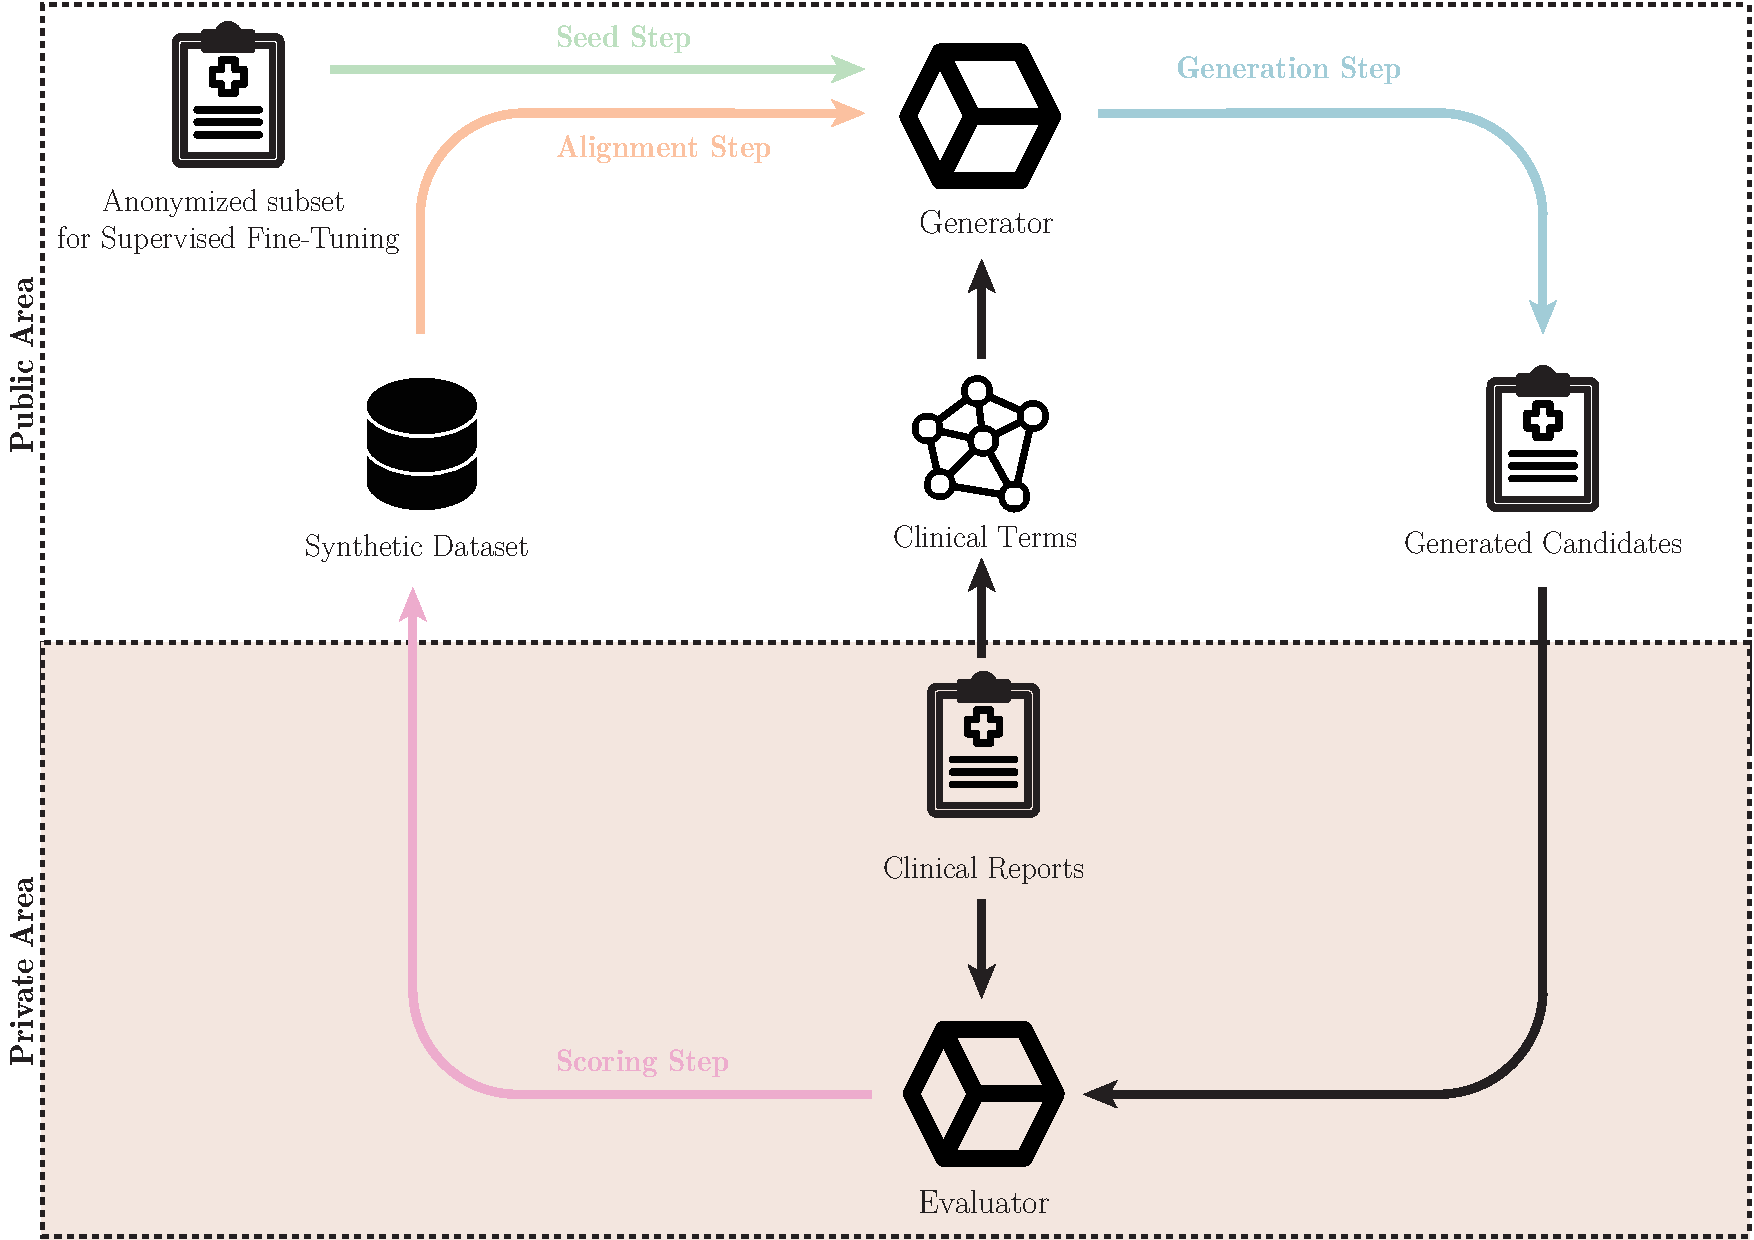
\includegraphics[width=1\textwidth]{figures/synthetic_generation_cl4health_2025/workflow.pdf}
    \caption{workflow of our approach}
    \label{fig:workflow}
\end{figure*}

\subsection{Example Outputs}
\newtcolorbox{modelinput}{colback=blue!5!white,colframe=blue!75!black}
\begin{figure}
\centering
\begin{modelinput}
\verb|<s>[INST]|As a doctor, you must write an original 'History of Present Illness' (HPI) section for a discharge summary.
Your response should capture the essence of a patient's health journey and recent medical experiences, while strictly using all the provided keywords conserving the order.
You must adopt a medical telegraphic style, abbreviated, characterized by concise and direct language.
\\
\textbf{Keywords:} \textit{metastatic, RCC, pancreas, reports, chills, tylenol, reports, rib pain, lying, chills, reports, dark stools, fever, zosyn, headache, contacts, anxious, pain, dysuria, joint pain, rash, hypotensive, asymptomatic, given, lactate, baseline, guaiac, stool, saw, stent, pancreatic, blood, tomorrow, treated, cholangitis, given, sat, ARF, reports, anxious}\verb|[/INST]|
\end{modelinput}
\caption{An example of prompt for the Figures \ref{appendix:ground},\ref{appendix:worst},\ref{appendix:best}}
\label{experiment:prompt}
\end{figure} 

\begin{figure}[!hbt]
    \centering
    \begin{modelinput}
    This is a 67 y.o male with h.o metastatic RCC to the pancreas,
recent ICU course for UGIB (12units pRBCs) who reports sudden
intermittent chills since wednesday for which he took tylenol.
Pt also reports R.side gnawing rib pain, while lying in bed
before the onset of chills. In addition, pt reports dark stools
for the last few days which started after taking "iron pills".
Pt states he went to [**Hospital1 2436**] ED because of a fever of 101.3,
however he felt better and did not want to wait to be seen. He
returned to [**Hospital1 2436**] today and was transferred to [**Hospital1 18**] after
a dose of zosyn, HCT 25. Pt denies headache/dizziness/blurred
vision, URI/cough, sick contacts, CP, +palp when anxious, -abd
pain/n/v/d/brbpr, dysuria/hematuria, joint pain, rash,
paresthesias. \\
. \\
At [**Hospital1 18**], pt found to be hypotensive to 75/40, asymptomatic. He
was given 3L IVF, lactate 6.8. HCT 22.8 from a baseline of 35 a
few weeks ago. He was found to have black, guaiac +stool. GI saw
pt, pt s/p stent to pancreatic ampulla, ?blocked  from blood.
Plan is to transfuse, ERCP tomorrow. ED also treated for
possible cholangitis/sepsis and pt was given dose of vanco.
Vitals 99.2, BP 99/66 HR 88 sat 98% on RA. Access 3PIV's 2,
20's, 18. Pt also found to be in ARF. \\
. \\
Currently, pt reports that he is anxious. \\
.
    \end{modelinput}
    \caption{An example of a ground truth associated with the prompt of Figure~\ref{experiment:prompt}}
    \label{appendix:ground}
\end{figure}

\begin{figure}[!hbt]
\centering
\begin{modelinput}
77 yo M w/ hx of metastatic RCC of the pancreas (pancreo-duodenal \\
mass reports R/o chills since starting [**6-2**] on [**2160-5-18**] (day 7-10 from \\
Hx. He has had fevers with taking tylenol at that time \\
(Ibuprofen 400mg, acetaminophen 650mg PRN for R/o rib pain and \\
steal). On [**2160-5-22**] he was lying in bed and became extremely \\
ill with chills. He reports this started a few minutes ago. Also \\
reports dark stools. His fever is 102F (38.3C), he is on 2g IV \\
zosyn (given IVF 2L NS, as he is V/5) for pneumonia with HC \\
reported by the Wife. He reports severe headache. He is not \\
compliant with PCP but has noticed many recent contacts with \\
his S/M. He is very anxious for relief of pain. He has some \\
dysuria and no joint pain. He has no rash. He is in the ED \\
actively pacing. He is hypotensive. He is BP 90/45 with 3+ pti \\
on his left hand. PRI all his vitals are stable otherwise at \\
BP 92/44 HR 81 RR 14 96 O2 Sat 99% RA. On ABG: pH 7.31, \\
PaCO2 28.1, PaO2 113. As a baseline (was done in ED), guaiac \\
in stool was positive. He was sent to CT with ortho in ED. Saw \\
his PCR [**Last Name (Only) **] [**Date**] [**Time (only) **] 5:15 and showed a 6.2mm x 5.1mm pancreatic \\
tail mass (blood in the head of the pancreas with no dilation \\
distally). He is scheduled for pancreatic stent placement \\
tomorrow. He was treated for acute cholangitis (e.g. given 3L NS \\
and 1g of IVF) and was given 1L NS to help with ARF. He \\
reports that he is more anxious for relief of pain.
\end{modelinput}
\caption{An example of synthetic data generated with Figure \ref{experiment:prompt} with a high \score}
\label{appendix:best}
\end{figure}

\chapter{Synthetic Document Generation: French Clinical Application}
\label{chap:french-application}

The previous chapters (\autoref{chap:synthetic} and \autoref{chap:privacy}) validated our synthetic generation methodology on English clinical data from \gls{mimic}-III.
A natural question follows: does this approach generalize to other languages and healthcare systems?

This chapter presents an industrial application of our methodology to French clinical documents, conducted in collaboration with Assistance Publique -- Hôpitaux de Paris (\gls{aphp}).
This work was led by Riccardo Tripodi as part of his master's thesis at Politecnico di Milano, adapting our generation pipeline to the French clinical context.
The results are encouraging and pave the way for larger-scale deployment within the \gls{aphp} infrastructure.

\minitoc

\section{Motivation and Context}

While the experiments presented in previous chapters demonstrate the effectiveness of our approach on English clinical data from \gls{mimic}-III, a critical question remains: does this methodology generalize to other languages and healthcare systems?
This consideration is particularly relevant given that the majority of clinical \gls{nlp} research focuses on English, leaving non-English healthcare systems underserved despite facing similar---or often greater---data scarcity and privacy challenges.

To address this question and validate our approach in a more applied setting, we conducted experiments on French medical reports in collaboration with Assistance Publique -- Hôpitaux de Paris (\gls{aphp}).
Beyond the language shift, this application involves clinical documents from a different medical context: while \gls{mimic}-III contains intensive care unit discharge summaries from a US academic hospital, the French corpus comprises diverse medical reports reflecting routine clinical practice across multiple hospital departments.

From a practical perspective, \gls{aphp} faces concrete challenges that motivate this work.
The hospital system seeks to deploy small, efficient models capable of classifying clinical documents for tasks such as automated \gls{icd} coding.
However, annotated training data remains sparse, and privacy regulations prevent direct use of patient records for model development.
Synthetic document generation addresses both constraints simultaneously.

Beyond immediate operational needs, this collaboration pursues broader research objectives.
First, generating high-quality synthetic documents enables sharing clinical data with the research community without compromising patient privacy---a significant step toward reproducible medical \gls{nlp} research in French.
Second, this work lays the groundwork for a longer-term goal: generating entirely synthetic patient records that preserve the statistical and clinical properties of real data while containing no actual patient information.

This setting presents several distinctive characteristics:

\begin{itemize}
    \item \textbf{Language and clinical conventions}: French clinical writing follows distinct conventions, with specific medical terminology, abbreviation patterns, and narrative structures that differ from English documentation practices.

    \item \textbf{Coding system}: French hospitals use \gls{icd}-10 codes rather than the \gls{icd}-9 codes present in \gls{mimic}-III, representing a different classification granularity.

    \item \textbf{Regulatory context}: European healthcare data is governed by \gls{gdpr}, imposing stringent requirements on data processing and transfer that make privacy-preserving approaches particularly valuable.

    \item \textbf{Fully synthetic seed corpus}: Unlike our \gls{mimic}-III pipeline, which required a small set of real pseudo-anonymized documents to bootstrap the generator (\autoref{chap:synthetic}), the French pipeline eliminates this dependency entirely.
    The seed corpus is generated synthetically from curated mappings between \gls{icd}-10 codes and medical keywords, using a large medical language model, without any real clinical document involved.
\end{itemize}

This cross-lingual validation thus serves multiple purposes: testing whether our methodology transfers across languages and clinical contexts, providing a practical solution for data-scarce healthcare systems, and opening pathways toward shareable synthetic medical corpora.

\section{Experimental Setup}

\paragraph{Dataset.}
The reference corpus used for scoring during \gls{dpo} refinement consists of fictive clinical reports written by practicing physicians across multiple hospital departments and medical specialties.
These documents are clinically realistic but contain no actual patient information, ensuring full reproducibility while eliminating any risk of privacy leakage.
Evaluation is performed on a strictly held-out test set of real clinical reports annotated by experts, fully disjoint from all data used in the pipeline.

\paragraph{Seed corpus generation.}
Prompts are constructed from a curated database linking \gls{icd}-10 codes to medically grounded French keywords describing symptoms, anatomy, treatments, and procedures.
Codes are sampled according to empirical hospital frequency distributions, and a constrained subset of associated keywords is selected for each prompt.
MedGemma-27B-IT~\citep{sellergren2025medgemma}, a large multilingual medical language model, generates \num{20000} synthetic clinical reports following a fixed eight-section narrative structure: \emph{Motif d'hospitalisation}, \emph{Antécédents}, \emph{Mode de vie}, \emph{Histoire de la maladie}, \emph{Examen clinique}, \emph{Examens complémentaires}, \emph{Évolution pendant l'hospitalisation}, and \emph{Conclusion}.
This seed corpus is entirely independent of real patient records, in contrast to the pseudo-anonymized seed documents used in our \gls{mimic}-III experiments (\autoref{chap:synthetic}).

\paragraph{Generator model.}
We employ Qwen3-4B-Instruct~\citep{yang2025qwen3} as the base generator model, selected for its strong multilingual capabilities and competitive performance on French text generation tasks.
Compared to Mistral-7B used in our \gls{mimic}-III experiments, Qwen3-4B offers a favorable trade-off between model size and generation quality for non-English languages.
The model is fine-tuned using \gls{lora}~\citep{hu2022lora} with rank $r=32$ and scaling factor $\alpha=64$, applied to all attention projection layers.
Training follows the same two-stage approach: initial supervised fine-tuning on the \num{20000} synthetic seed documents, followed by three iterations of \gls{dpo} alignment.

\paragraph{Privacy-bounded refinement.}
During \gls{dpo} iterations, the generator produces candidate reports that are scored against the fictive reference documents inside the hospital infrastructure.
For each keyword prompt, $N=4$ candidates are generated using a mixed temperature strategy: one sample at $\tau = 0.2$ to favor coherent outputs, and three samples with temperatures drawn from $\mathcal{U}(0.6, 0.9)$ to encourage diversity.
Keywords are extracted from reference reports using QuickUMLS~\citep{soldainiQuickUMLSFastUnsupervised2016}.
The complete scoring mechanism is detailed in \autoref{sec:french-scoring}.

\paragraph{Downstream task.}
We evaluate synthetic document quality through \gls{icd}-10~\citep{who_icd10} multilabel classification, mirroring our \gls{icd}-9 experiments on \gls{mimic}-III.
A ModernBERT-large classifier~\citep{warner2025smarter} is trained exclusively on synthetic datasets of varying sizes (\num{10000}, \num{20000}, \num{50000} documents) and evaluated on the held-out real test set.
Classification targets are defined by the top-$k$ most frequent \gls{icd}-10 codes with $k \in \{20, 50, 100\}$.
At the \num{10000} scale, this yields approximately \num{350} samples per code for top-20 but only \num{150} for top-100.
The average number of codes per document increases with $k$: $1.52 \pm 0.82$ for top-20, rising to $2.10 \pm 1.14$ for top-100.
Generated reports average approximately $800 \pm 240$ words across refinement stages.

\section{Scoring Mechanism}
\label{sec:french-scoring}

While our \gls{mimic}-III experiments relied primarily on SemScore for document quality assessment, the French application employs a composite scoring mechanism combining two complementary components.

\paragraph{Semantic similarity.}
The first component measures cosine similarity between synthetic and reference documents using BioLORD-2023-M~\citep{remy2024biolord} embeddings.
Unlike general-purpose embedding models, BioLORD integrates clinical knowledge graph information, making it particularly suitable for assessing semantic fidelity in medical documents across languages.

\paragraph{\gls{llm}-as-judge.}
The second component uses Qwen3-30B-A3B-Instruct~\citep{yang2025qwen3} as an \gls{llm}-as-judge to evaluate medical correctness and content alignment of the generated candidate with respect to the reference report.

\paragraph{Composite score.}
The final quality score combines these two components through simple averaging:
\begin{equation}
    S_{composite} = \frac{1}{2}\left(S_{similarity} + S_{judge}\right)
\end{equation}
This composite score guides candidate selection during \gls{dpo} alignment, with higher-scoring documents serving as preferred examples and lower-scoring ones as rejected examples.
Compared to the SemScore-only approach used on \gls{mimic}-III, this two-faceted evaluation provides a stronger training signal by capturing both semantic fidelity and clinical plausibility.

\section{Example of Generated Report}

\autoref{fig:french-example} presents an excerpt of a synthetic French clinical report generated at the end of the pipeline (after DPO3).
The document follows the eight-section narrative structure and demonstrates clinically coherent content with appropriate medical terminology.

\begin{figure}[htb]
\centering
\begin{tcolorbox}[colback=gray!5,colframe=gray!50,boxrule=0.5pt,arc=2pt,left=8pt,right=8pt,top=6pt,bottom=6pt,fontupper=\small]
\textbf{Motif d'hospitalisation:}
Mme Dupont, 68 ans, est admise en hospitalisation de jour le 15/03/2024 pour traitement d'une angiodermite nécrotique extensive surinfectée. Cette lésion cutanée chronique, initialement diagnostiquée il y a plusieurs années, s'est aggravée de manière significative, nécessitant une prise en charge intensive et une surveillance rapprochée.\\[0.5em]

\textbf{Histoire de la maladie:}
L'angiodermite nécrotique initiale de Mme Dupont a connu des épisodes récurrents et des aggravations progressives au fil des ans. Depuis environ 6 mois, une lésion cutanée extensive, initialement localisée au niveau des membres inférieurs, s'est étendue progressivement et s'est caractérisée par une nécrose cutanée et une infection bactérienne sévère. La lésion est devenue très douloureuse, avec des signes d'inflammation marquée (érythème, chaleur, \oe{}dème) et une ulcération profonde. La patiente a consulté son dermatologue qui a initié un traitement antibiotique (Ceftriaxone) et une antibiothérapie topique, mais l'aggravation persiste.\\[0.5em]

\textit{[\ldots]}\\[0.5em]

\textbf{Mots-clés:} Angiodermite nécrotique extensive surinfectée, personne vivant seule à son domicile.
\end{tcolorbox}
\caption{Excerpt of a synthetic French clinical report generated after three \gls{dpo} iterations. The document follows the standardized eight-section structure and demonstrates clinically coherent content.}
\label{fig:french-example}
\end{figure}

\section{Results}
\label{sec:french-results}

Table~\ref{tab:french-results} presents classification performance across dataset sizes and \gls{dpo} iterations.
We report macro F1 scores on the held-out test set, with relative gains computed against the Step0 baseline (\gls{sft} only, no \gls{dpo} alignment).

\begin{table}[htb]
\centering
\begin{tabular}{@{}llccccr@{}}
\toprule
\textbf{Dataset} & \textbf{Top-k} & \textbf{Step0} & \textbf{DPO1} & \textbf{DPO2} & \textbf{DPO3} & \textbf{Gain} \\
\midrule
\multirow{3}{*}{10K}
    & 20  & 0.389 & \textbf{0.422} & 0.422 & 0.418 & +7.4\% \\
    & 50  & 0.250 & 0.294 & 0.302 & \textbf{0.317} & +26.9\% \\
    & 100 & 0.175 & 0.197 & 0.202 & \textbf{0.238} & +36.5\% \\
\midrule
\multirow{3}{*}{20K}
    & 20  & 0.438 & \textbf{0.457} & 0.448 & 0.447 & +2.1\% \\
    & 50  & 0.299 & 0.326 & 0.334 & \textbf{0.347} & +16.2\% \\
    & 100 & 0.195 & 0.230 & 0.210 & \textbf{0.285} & +45.8\% \\
\midrule
\multirow{3}{*}{50K}
    & 20  & 0.445 & \textbf{0.461} & 0.461 & 0.455 & +2.3\% \\
    & 50  & 0.326 & 0.351 & \textbf{0.385} & 0.383 & +17.6\% \\
    & 100 & 0.230 & 0.268 & 0.300 & \textbf{0.316} & +37.2\% \\
\bottomrule
\end{tabular}
\caption{Classification F1 scores on French \gls{icd}-10 multilabel task across dataset sizes and \gls{dpo} iterations.
Relative gains computed against Step0 baseline.}
\label{tab:french-results}
\end{table}

The results reveal consistent patterns that mirror our \gls{mimic}-III findings while demonstrating even stronger improvements from \gls{dpo} alignment.
Relative gains range from +2\% for top-20 to +46\% for top-100, substantially higher than the +3\% to +6\% gains observed on English data.
This difference likely stems from the composite scoring mechanism combining semantic similarity and \gls{llm}-as-judge, which provides a richer training signal for preference optimization compared to SemScore alone.

The relationship between task complexity and \gls{dpo} benefit follows the same pattern as \gls{mimic}-III.
For top-20 classification, a single \gls{dpo} iteration often suffices, with subsequent iterations providing marginal or no additional improvement.
In contrast, top-50 and top-100 configurations benefit from continued alignment through DPO2 and DPO3, confirming that rare label prediction requires higher-quality synthetic documents regardless of language.

Dataset scaling effects remain consistent: 50K models outperform 20K and 10K counterparts across all configurations.
However, the most striking observation is that even the smallest 10K dataset with DPO3 alignment achieves competitive performance, suggesting that quality-focused generation can partially compensate for limited data quantity.

\section{Cross-lingual Comparison}
\label{sec:crosslingual}

To assess whether our methodology exhibits consistent behavior across languages, we compare key patterns between the English (\gls{mimic}-III) and French (\gls{aphp}) experiments.

The qualitative patterns are remarkably consistent across both languages.
In both settings, \gls{dpo} alignment provides clear benefits over the \gls{sft} baseline, with gains concentrated in higher top-k configurations where rare labels dominate.
The diminishing returns pattern for simpler tasks (top-20) appears in both experiments, with DPO1 often providing the best results before subsequent iterations plateau.
Iterative \gls{dpo} through DPO2 and DPO3 proves beneficial for complex tasks (top-100) in both languages, and dataset scaling consistently improves absolute performance.

The quantitative differences are notable: French experiments show substantially larger relative improvements from \gls{dpo} alignment (+36\% to +46\% for top-100) compared to English (+3\% to +6\%).
We attribute this primarily to the composite scoring mechanism employed in the French pipeline, which combines semantic similarity and \gls{llm}-as-judge evaluation.
This two-component scoring likely provides a stronger training signal for preference optimization compared to the SemScore-only approach used on \gls{mimic}-III.

Additional factors may contribute to these differences: the Qwen3-4B model may respond more favorably to \gls{dpo} than Mistral-7B, and \gls{icd}-10 classification may present different challenges than \gls{icd}-9.
However, the consistent qualitative patterns across languages provide strong evidence that the core methodology---keyword-guided generation with iterative preference optimization---transfers effectively regardless of these implementation details.

\section{Discussion \& Conclusion}

These results provide strong evidence that our reward-based synthetic generation approach generalizes effectively beyond English.
The consistent improvement patterns observed across \gls{mimic}-III and \gls{aphp} experiments---despite differences in language, coding systems, and model architectures---suggest that the underlying methodology captures language-agnostic principles of clinical document structure.

From a practical standpoint, this cross-lingual validation is promising for the medical domain.
Healthcare systems worldwide face similar challenges: sensitive patient data that cannot be shared, sparse annotations, and regulatory constraints on data processing.
Our results demonstrate that synthetic document generation offers a viable pathway to address these challenges regardless of language, opening opportunities for medical \gls{nlp} research in underserved linguistic communities.

Looking forward, the collaboration with \gls{aphp} opens perspectives for extending this work.
One objective is the generation of entirely synthetic patient records, leveraging the multimodal data available in hospital information systems to create coherent document collections that span a patient's clinical trajectory.
Another direction concerns long-context generation: current experiments focus on relatively short documents, and scaling to longer clinical narratives such as complete discharge summaries or multi-document patient histories remains to be explored.

\paragraph{Acknowledgements.}
This work on French clinical data was conducted in collaboration with Assistance Publique -- Hôpitaux de Paris (\gls{aphp}).
We thank Riccardo Tripodi for implementing and running the experiments on French medical reports.

\chapter{Weak Supervision for Clinical Natural Language Processing}

In clinical and other specialized domains, data are scarce due to their confidential nature. This lack of data is a major problem when fine-tuning language models.
Nevertheless, very large language models (LLMs) are promising for the medical domain but cannot be used directly in healthcare facilities due to data confidentiality issues. We explore an approach of annotating training data with LLMs to train smaller models more adapted to our problem. 
We show that this method yields promising results for information extraction tasks.

\section{Introduction}
Clinical notes contain the interactions between the patient and healthcare staff. Professionals record their impressions, observations, and various medical procedures performed. Despite the computerization of clinical documents, notes should remain fairly expressive and in a free format to save time for healthcare personnel and allow for the description of unusual situations \citep{Rosenbloom2011DataDocumentation}. Moreover, a large amount of crucial information is exclusively contained in clinical notes. According to a study by \citet{Escudie2017ADisease}, approximately 80\% of patient phenotypes (a set of observable biological and physical characteristics that can characterize a disease) are present only in free text. These documents are difficult to use without advanced methods such as deep learning in NLP. The use of such methods requires the collection and annotation of a significant amount of medical data. However, \citet{Fries2022DatasetModeling} proposes the term "\emph{dataset debt}," highlighting that learning data in the biomedical field is poorly accessible, poorly documented, and opaque as to its reusability in a commercial or a hospital context. According to the article, only 13\% of the 167 analyzed datasets are accessible and downloadable, 22\% use a standard structured format, and 40\% are in the public domain.
In recent years, large language models (LLMs) have proved their ability to perform a wide range of tasks with high accuracy in a zero-shot or a few-shots contexts.
This trend holds great potential for clinical NLP, as preliminary results show promise for information extraction tasks \citep{Agrawal2022LargeExtractors}. 
However, the clinical domain presents unique challenges due to the confidential and linguistically specific nature of its data, which can make collection and annotation time-consuming and expensive.
Using LLMs for efficient information extraction without training data could be attractive, but it raises confidentiality concerns.
The model deployment should be controllable, and the model's predictions should evolve to fit a specific and changing annotation guideline.
Most multilingual LLMs are not freely available \citep{Scao2022BLOOM:Model,Ouyang2022TrainingFeedback,Thoppilan2022LaMDA:Applications}, to the best of our knowledge, only BLOOM is open-source and deployable in a custom infrastructure. The computing resources to use these models remains challenging for healthcare establishments.     

One approach to address these issues is to distil LLMs into a smaller model via weak supervision. 
Weak supervision has recently gained community attention because it alleviates the annotation task. This technique refers to annotating datasets using rule-based, heuristic, dictionary extraction or more advanced methods and then training the smaller model on this dataset.
In the same way, knowledge distillation aims to transfer knowledge from a master model to a student model. It has often been used to compress large-scale models to improve memory footprint and the inference speed \citep{Li2021DynamicModels}. 
Moreover, student models trained through knowledge distillation can be more easily monitored and versioned. Hosting them increases the healthcare centre's sovereignty, and they become more compliant with existing privacy policies, as input data or predictions don't leave the building.

\section{Motivation and Contributions}
We study the use of LLMs in the knowledge distillation technique via weak supervision in the Multilingual Clinical domain, especially in clinical entity extraction. We extend the \citet{Agrawal2022LargeExtractors} study in the sense that we propose an in-depth study of the use of \instruct to annotate a training dataset. Our work\footnote{codebase: \url{https://github.com/arkhn/bio-nlp2023}.} mainly aims to compare the annotation quality using weak supervision tasks on a smaller model (Figure \ref{fig: motiv}). Finally, we propose to combine annotations provided by \instruct and the dictionary extraction method.

This takes form in these contributions:
\begin{itemize}
    \item We show that \instruct distillation (Figure \ref{fig: motiv} middle) is a competitive technique compared to classic weak-supervision techniques in a multilingual clinical domain;
    \item We propose a weak supervision approach (Figure \ref{fig: motiv} bottom) that combines annotations from dictionary extraction and \instruct, which outperform the approach with only \instruct annotation.
\end{itemize}

\begin{figure*}[htp!]
\centering
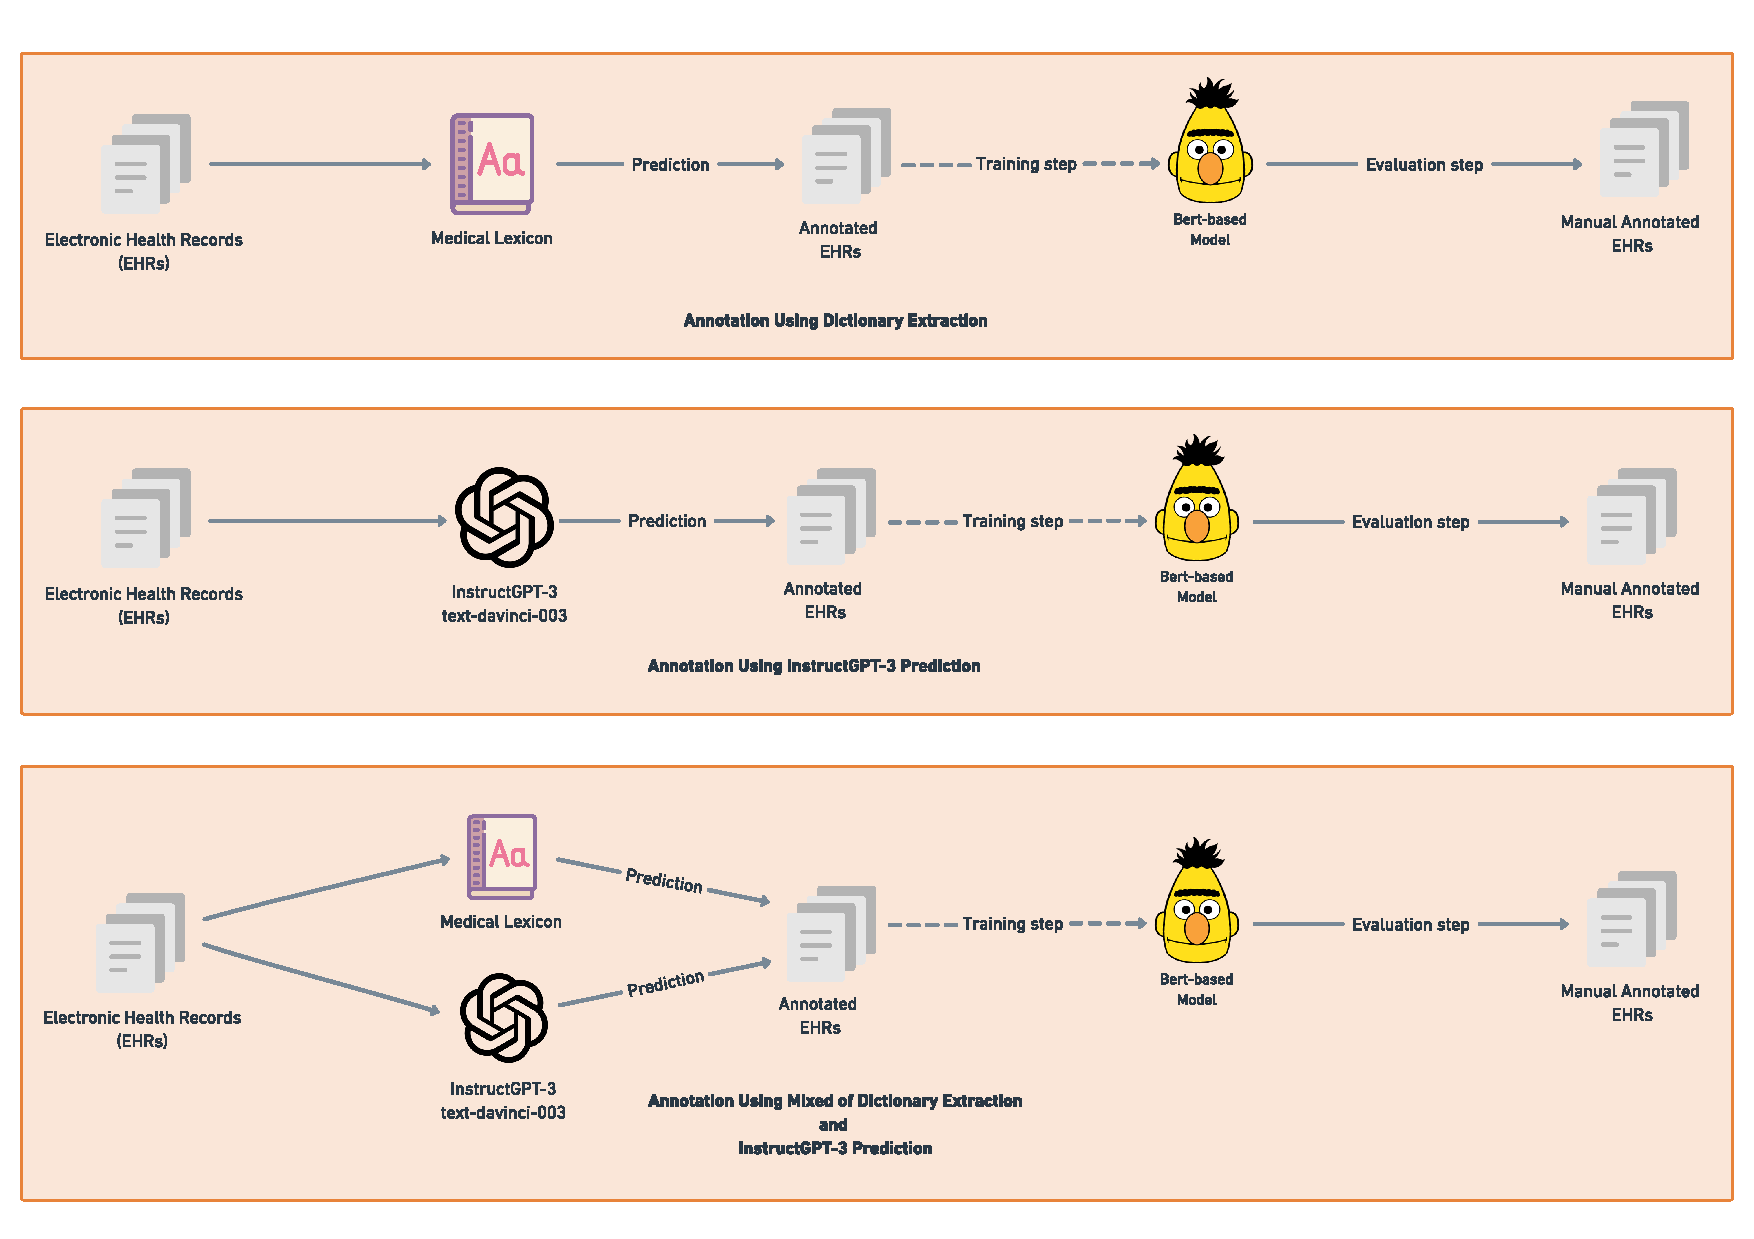
\includegraphics[width=0.9\textwidth]{figures/multi_weak_supervision/workflow.pdf}
\caption{The different workflows we experiment with. The last workflow used a combination of \instruct and dictionary annotations; we tested different proportions of these annotations as described in \ref{sec:prot}.}
\label{fig: motiv}
\end{figure*}

\section{Related Works}
\paragraph{Weak Supervision} deep learning approach has achieved remarkable success in several domains beyond NLP \citep{Zhang2022ASupervision}. However, the main bottleneck is collecting massively annotated data. To address this issue, weak supervision replaces ground-truth annotation with automatic annotation based on heuristic rules, gazetteers or constraints linguistic rules to address. Some techniques called \textit{distant supervision} exploit semantic links from knowledge bases or ontologies \citep{Lison2021Skweak:NLP}. \citet{Karamanolakis2021Self-TrainingSupervision} proposes an iterative self-training method to combine classic weak supervision and inference of the learning model to extract entities not covered by the initial heuristic rules. In the clinical domain, weak supervision has already been used for specific use cases \citep{Cusick2021UsingIdeation,Fries2021Ontology-drivenRecords,Wang2019ARepresentation}.
\paragraph{Clinical Language Models} In the clinical context, some specific terms are underrepresented or absent in the general domain. As a result, the clinical NLP community has pretrained Language Models (LMs) \citep{Alsentzer2019PubliclyEmbeddings, Lee2020BioBERT:Mining,Alsentzer2019PubliclyEmbeddings} over domain-specific corpora (i.e. MIMIC-III \citep{Johnson2016MIMIC-IIIDatabase}, Pubmed abstracts). These models could be trained from scratch or from checkpoint to specialize a domain-agnostic model \citep{Gururangan2020DontTasks}.

Though, the performance gains are marginal compared to the general language model. The structure and the abbreviated text present in clinical notes hurt performance.
Instead of pretraining a specialized clinical model, machine learning practitioners can fine-tune agnostic-domain LLMs such as the GPT family of models or T5 on the clinical task. Fine-tuned general-purpose models have proven effective in clinical question-answering, protected health information de-identification, and relation extraction \citep{Lehman2023DoModels}. But this approach requires an important infrastructure and a regular re-finetuning if the data distribution of the EHR shifts. Nevertheless, some LLMs have been trained from scratch over clinical domain-specific notes such as GatorTron \citep{Yang2022ARecords}, BioGPT \citep{Luo2022BioGPT:Mining} or ClinicalT5 \citep{Lu2022ClinicalT5:Text} who achieved promising performance on several tasks.
Additionally, in-context learning with agnostic LLMs such as \instruct \citep{Ouyang2022TrainingFeedback} where no weight is modified shows good results \citep{Agrawal2022LargeExtractors, Brown2020LanguageLearners} and outperforms specialized smaller models on several clinical tasks.
\paragraph{Prompt-based Method}
Prompt-based learning for generative language model treats a downstream task as a language modelling problem where a language model predicts the next tokens of the instruction given a textual prompt \citep{Sainz2021LabelExtraction}.

In this paradigm, instead of fine-tuning a model to a downstream task (\textit{"pre-train, fine-tune and predict"}), we manipulate the behaviour of a pretrained LM using an appropriate prompt to give the desired output (\textit{"pre-train, prompt and predict"}). 
\textit{prompt engineering} explores the most suitable prompt method applied to a LM to solve a task.
This way, an unsupervised pre-trained LM can be used for many tasks \citep{Liu2023Pre-trainProcessing}.

Among these methods, \textit{in-context learning} is the most popular method for information extraction, question-answering or sentiment analysis. In the clinical domain, some works exist on information retrieval and question-answering. The prompt contains three components: the examples' template, the set of examples and the ordering of prompts, such as present in Figure \ref{fig:prompt}. The aim is to provide some training examples in the prompt before the test example. However, the chosen examples and their ordering and the format could impact performance \citep{Zhao2021CalibrateModelsb}; these three components must be tuned to optimize performance.

In another way, we can cite works around the chain of thoughts (CoT). This encourages the LLM to explain its reasoning to get more accurate results, especially in mathematical and logical reasoning \citep{Wei2022ChainModels, Cobbe2021TrainingProblems}. This technique could be used with reason edited manually in the prompt or with two separate prompts where the first involves a reasoning task, then concatenated with the second prompt involving the main tasks.

Other techniques involve generated knowledge similar to CoT. Instead of reasoning, the first prompt generates potentially useful information associated with the tasks concatenated in the final prompt \citep{Liu2022GeneratedReasoning}.

\section{Method}

\subsection{Creating Annotations and Knowledge Distillation via Weak Supervision}
\paragraph{Annotation Extraction from LLM Output}
Our study is inspired by the method developed in this paper \citep{Agrawal2022LargeExtractors}. Their works benchmark how \instruct \citep{Ouyang2022TrainingFeedback} perform clinical NLP tasks in English. They show that \instruct performs well in several clinical tasks. They introduce 3 new datasets to benchmark few-shot clinical information extraction to achieve this. Also, they introduce \textit{guided prompt design} to induce easy-to-structure output with resolvers (or parsers) to convert the output into a structured prediction easily. 
Our work differs in the following: 
\begin{enumerate}
    \item Our studies areas are knowledge distillation via weak supervision and the improvement of this technique combining annotations from LLMs and dictionary extraction;
    \item our methods are applied in a multilingual context, the initial work was only done in English;
    \item we focus on the clinical entities extraction task based on the E3C dataset guidelines.
\end{enumerate}


In this work, the LLM is used only as a predictor; we only query the model, no additional fine-tuning step has been realized, and we can only access inference parameters such as temperature, top p, frequency or presence penalty. We set the \textit{temperature} and \textit{top p} to 0 to control randomness and have a deterministic behaviour. So as not to penalize repetitions, we set the \textit{presence penalty} and \textit{frequency penalty} to 0. We use an InstructGPT-3 model (text-davinci-003) \citep{Ouyang2022TrainingFeedback} to infer the whole annotations for all our experiments.
We provide the model with an instruction concatenated by the example to be predicted (Figure \ref{fig:prompt}). The output of \instruct is a string of characters that we must structure to align the predicted clinical entities with the initial text (Figure~\ref{fig:formalization}).

 The task is to annotate the words (or tokens) of a sentence $x \in \Sigma^*$ with a set of labels such that $L=\{O, B_\text{clin}, I_{\text{clin}}\}$ where O denotes a word in the text without a label, \bclin the first word of a clinical entity and \iclin the following words according to the format \textit{IOB} \citep{Ramshaw1995TextLearning}. The goal is to identify the labels O, \bclin, \iclin and their character offsets in the sentence $x$. The task output is defined as $\hat{y}=[ y_1, y_2, \ldots, y_n ] \in Y$, where $\hat{y}$ is the set of predicted annotations, and $y_i= \langle s_i, e_i, l_i
\rangle$ such that $s_i$ is the start offset, $e_i$ is the end offset and $l_i\in L$ of the $i^{th}$ annotation.
\begin{figure*}
\centering
\resizebox{1\textwidth}{!}{
\fbox{
\begin{minipage}[c][2.2in]{\linewidth}
\begin{small}
\begin{align*}
    & x = \texttt{'The patient had presented a progressive deterioration of the general condition,}\\
    & \qquad \texttt{a fever and night sweats.'}\\
    & p = concat(t, x)\\
   & \begin{aligned}
        o = \Phi(p, \theta_h) = & \texttt{'-"fever" } \\ 
                                & \texttt{-"night sweats"'}
      \end{aligned}\\
    & \begin{aligned}
        r(o, x) = & \; [ \\ 
                         & \space\space(\texttt{The}, 0 , 3, O), (\texttt{patient}, 4 , 11, O), \dots, \\ 
                         & \space\space(\texttt{fever}, 72, 77, B_{clin}), (\texttt{and}, 79, 82, O), \\
                         & \space\space(\texttt{night}, 83, 87, B_{clin}), (\texttt{sweats}, 88, 94, I_{clin}), \dots \\
                         & ]
      \end{aligned}
\end{align*}
\end{small}
\end{minipage}}
}
    \caption{our method's prediction and structuring steps on an example. The $t$ template is illustrated in Figure \ref{fig:prompt}.}
    \label{fig:formalization}
\end{figure*}

As mentioned, a prompt-based method requires concatenating a template $t \in \Sigma^*$ with our sentence $x$ to give our prompt, such as $p=concat(t,x)$. 
We produce our output $o \in \Sigma^*$ from our LLM model $\Phi$ such as $o=\Phi(p, \theta_h)$, where $\theta_h$ represents the set of hyperparameters (\textit{temperature}, \textit{top p}, \textit{frequence penalty}, \textit{presence penalty}).

Then, we structure $o$ such as $\Sigma^* \rightarrow Y$ using a simple string-matching function to produce a set of labels $\hat{y}$ where $r$ is our resolver applying the string matching function: $r(o, x)=\hat{y}$.

\paragraph{Knowledge Distillation via Weak Supervision} Finally, the annotations generated via \instruct prediction are used as a training dataset to fine-tune a smaller language model to a NER downstream task. For smaller language models, we limit our study to encoder models as mentioned in Table~\ref{tab:models}.

\subsection{Prompting}

We prime the model with three annotated data points, each corresponding to a sentence from our corpus (Table \ref{tab:counts}).
For each language, we try 3 sets of data points. For each of them, we test the F1-Score performance of \instruct on the test dataset (\layerOne), and we select the set with the best F1-Score to perform prediction on the unannotated dataset. 
 We insert keywords associated with the E3C guideline definition of the clinical entities into prompts. 
 We add guidance to explicit the response structure to facilitate parsing the output \citep{Agrawal2022LargeExtractors} (Figure \ref{sec:prot}).

\section{Experiments}
\subsection{Dataset}
We use the annotated E3C multilingual dataset \citep{Magnini2020TheCases} for our experiments, consisting of two annotation types: temporal and clinical entities. The languages supported are English (en), Basque (eu), Spanish (es), French (fr) and Italian (it). Clinical entities are identified as patient disorders which could map to the UMLS meta thesaurus. The annotators have linked extracted clinical entities and UMLS concepts. In our experiments, we only extract clinical entities without mapping UMLS concepts. 
The E3C dataset is organized into 3 layers. A layer consists of a subset of files from each language annotated in a certain way (manually, semi-automatically) depending on the layer:
\begin{itemize}
    \item the first layer (\layerOne) consists of the full manual annotation; we used this layer as a test set for our experiments;
    \item The second layer consists of semi-automatic annotation; we use this layer as a train set with the initial annotation or the annotation inferred by InstructGPT-3. Moreover, we have access to two states of this layer; the first is the layer entirely annotated with dictionary extraction (\layerTwo); the second is a subset of this layer (only $10\%$) that has been fixed manually (\layerValidate). The dictionary contains terms from UMLS and terms extracted from \layerOne;
    \item Finally, the third layer (\layerThree) is unannotated, which we don't use for our experiments.
\end{itemize}

As mentioned above, the E3C dataset is well-suited for our weak-supervision studies. But, the dataset has limited data in its various layers (Table \ref{tab:counts}). To address this limitation, we divide \layerTwo into five parts using 5-fold cross-validation. For \layerValidate, we use the entire data as the training set. Our experiments employ multiple models for each language and relied solely on \verb|xlm-roberta-base| in a multilingual context. The results presented in our work are an aggregation of the means and standard deviations across models and folds.
However, each experiment result and model are reported in Appendix \ref{section:app}.

\subsection{Experimental Setup} 
\label{sec:prot}
We conduct experiments on the clinical entity extraction tasks. For each language, we use models mentioned in Table \ref{tab:models} as a student model for the knowledge distillation step.
\begin{table}
    \centering
    \small
    \resizebox{1\columnwidth}{!}{
        \begin{tabular}{@{}ll@{}}%
\toprule%
Language&Models\\%
\midrule%
en&\verb|emilyalsentzer/Bio_ClinicalBERT| \citep{Alsentzer2019PubliclyEmbeddings}\\%
&\verb|roberta-base| \citep{Liu2019RoBERTa:Approach}\\%
&\verb|xlm-roberta-base| \citep{Conneau2019UnsupervisedScale} \\%
\midrule%
es&\verb|BSC-LT/roberta-base-biomedical-es| \citep{Carrino2022PretrainedSpanish}\\%
&\verb|dccuchile/bert-base-spanish-wwm-cased| \citep{Ca2020SPANISHDATA}\\%
&\verb|xlm-roberta-base| \\%
\midrule%
eu&\verb|ixa-ehu/berteus-base-cased| \citep{Agerri2020GiveBasque}\\%
&\verb|xlm-roberta-base| \\%
\midrule%
fr&\verb|Dr-BERT/DrBERT-7GB| \citep{Labrak2023DrBERT:Domains}\\%
&\verb|camembert-base| \citep{Martin2019CamemBERT:Model}\\%
&\verb|xlm-roberta-base| \\%
\midrule%
it&\verb|dbmdz/bert-base-italian-cased| \citep{Schweter2020ItalianModels}\\%
&\verb|xlm-roberta-base| \\\bottomrule%
%
\end{tabular}
    }
    \caption{The models used for each language during our experiments. We mention in this table the name of the model in the huggingface model repository}
    \label{tab:models}
\end{table}
We conduct our experiments we use five different dataset settings. For \textbf{Monolingual Setting} (\SettingD), \textbf{Gold Setting} (\SettingB), \textbf{\SettingD~$\cap$~\SettingB} (\SettingC) and each language, we use the \layerTwo of the corresponding language. For the \textbf{Multilingual Setting} (\SettingE) and each language, we concatenate the \layerTwo of the whole languages in E3C to constitute the train set. Finally, for all settings and each language, we test our method on the \layerOne of the language we experiment with.
\begin{itemize}
    \item \textbf{Monolingual Setting} (\SettingD): We use a ratio $r$ to control the mix of annotations, with $r$ representing the proportion of annotations from dictionary extraction and $(1-r)$ representing the proportion of annotations from \instruct. If $r=1$, the models are trained using only \instruct annotations, while if $r=0$, the models are trained exclusively with \dict annotations. We test and compare the performance of the trained models using various ratio values of $r$. 
    \item \textbf{Gold Setting} (\SettingB): we use \layerValidate\space as the train set, and we compare encoder models trained on manually corrected annotation ($r=0$) and an encoder model trained on the same subset but using \instruct prediction annotations ($r=1$);
    \item \SettingC :  we use \layerTwo as the train set. Still, we replace weak-supervision annotations with the annotation fixed in \layerValidate. So, a small part of the \instruct prediction annotations and the dictionary extraction annotations has been replaced by manual annotations;
    \item \textbf{Multilingual Setting} (\SettingE): we use the same setting as \SettingD except we are on multilingual training context. For this setting, our trained models are multilingual language models. We use \verb|xlm-roberta-base|. 
\end{itemize}

\subsection{Results}
\paragraph{\instruct Prediction Analysis} For \layerTwo, we observe that \instruct extracts more entities than original extraction (Table~\ref{tab:counts}). This trend is reduced in English and Spanish even if we observed a more important quantity of \iclin in tokens annotated by \instruct for all languages. 
For \layerValidate, the quantity of tokens annotated by both methods (\instruct vs manually corrected annotation) is relatively equivalent. 

\begin{table}
\centering
\large
\resizebox{1\columnwidth}{!}{
\begin{tabular}{@{}ccccccccc@{}}%
\toprule%
Language&Layer&Tokens&\multicolumn{2}{c}{\bclin}&\multicolumn{2}{c}{\iclin}&\multicolumn{2}{c}{\bclin $+$ \iclin}\\%
&&&\textit{\dict}&\textit{\instruct}&\textit{\dict}&\textit{\instruct}&\textit{\dict}&\textit{\instruct}\\%
\midrule%
en&\Ssilver&58520&\textbf{2134}&1438&1036&\textbf{1595}&\textbf{3170}&3033\\%
&\Sval&6646&\textbf{254}&149&\textbf{137}&130&\textbf{391}&279\\%
\midrule%
es&\Ssilver&57065&\textbf{2625}&2245&1298&\textbf{1857}&3923&\textbf{4102}\\%
&\Sval&6291&\textbf{329}&236&\textbf{269}&159&\textbf{598}&395\\%
\midrule%
eu&\Ssilver&18365&482&\textbf{800}&63&\textbf{482}&545&\textbf{1282}\\%
&\Sval&4819&\textbf{327}&207&\textbf{245}&143&\textbf{572}&350\\%
\midrule%
fr&\Ssilver&59998&2013&\textbf{2402}&840&\textbf{2239}&2853&\textbf{4641}\\%
&\Sval&6452&267&\textbf{295}&\textbf{244}&225&511&\textbf{520}\\%
\midrule%
it&\Ssilver&60248&1643&\textbf{2099}&793&\textbf{1628}&2436&\textbf{3727}\\%
&\Sval&6538&\textbf{224}&223&147&\textbf{199}&371&\textbf{422}\\\bottomrule%
%
\end{tabular}
}
\caption{The number of annotated tokens for each annotation type for the \layerTwo ($l_{2}$) and \layerValidate ($l_{val}$). The notation \textit{Gold} corresponds to the original extraction, and the notation \textit{GPT} correspond to the \instruct annotation.}
\label{tab:counts}
\end{table}

\paragraph{Knowledge Distillation Evaluation} We compare the distilled model and \instruct on the \layerOne (Table \ref{tab:distilation}). Distillation is beneficial in terms of performance for Basque, French and Italian. Moreover, we denote a remarkable gap between \instruct ($0.63$) and distilled models ($0.75$) in Italian. Spanish and English have reversed trends: \instruct performs better than distilled models. This echoed the exception we observed in the \textbf{\instruct Prediction Analysis} paragraph.

\begin{table}
    \centering
    \small
    \resizebox{1\columnwidth}{!}{
        \begin{tabular}{@{}ccc@{}}%
\toprule%
\small
Language&\multicolumn{2}{c}{F1-Score}\\%
&\instruct&\distilmodels\\%
\midrule%
en&\textbf{0.71}&0.66 \bm{$\pm$} 0.01\\%
es&\textbf{0.74}&0.70 \bm{$\pm$} 0.02\\%
eu&0.60&\textbf{0.61 \bm{$\pm$} 0.04}\\%
fr&0.74&\textbf{0.75 \bm{$\pm$} 0.01}\\%
it&0.63&\textbf{0.75 \bm{$\pm$} 0.01}\\\bottomrule%
%
\end{tabular}
    }
    \caption{The mean F1-score of the models for each language in E3C using {\layerOne~} as evaluation set. We evaluate the direct output of {\instruct} and the aggregated mean score of each model for each language listed in Table \ref{tab:models} using \SettingA and {\instruct} annotation as a train set.}
    \label{tab:distilation}
\end{table}

\paragraph{\SettingA} If we compare the global F1-Score (Table \ref{tab:global}), the \distilmodels ($r=1$) perform better than the \weakModel ($r=0$) trained. 
In detail, {\distilmodels} display a better recall and recognizes multi-word clinical terms more easily. Still, this flexibility, balanced by the too-biased detection of false positive terms, lowered the precision score. In comparing {\distilmodels} versus {\weakModel} (Figure \ref{fig:setting_A}), we note a noticeable performance gain of almost $0.1$ in Basque, followed by French and Italian. In English, the F1-score of both models is relatively equivalent. For Spanish, the \weakModel outperformed the {\distilmodels} and still has our highest F1-Score.
\begin{figure}
    \centering
    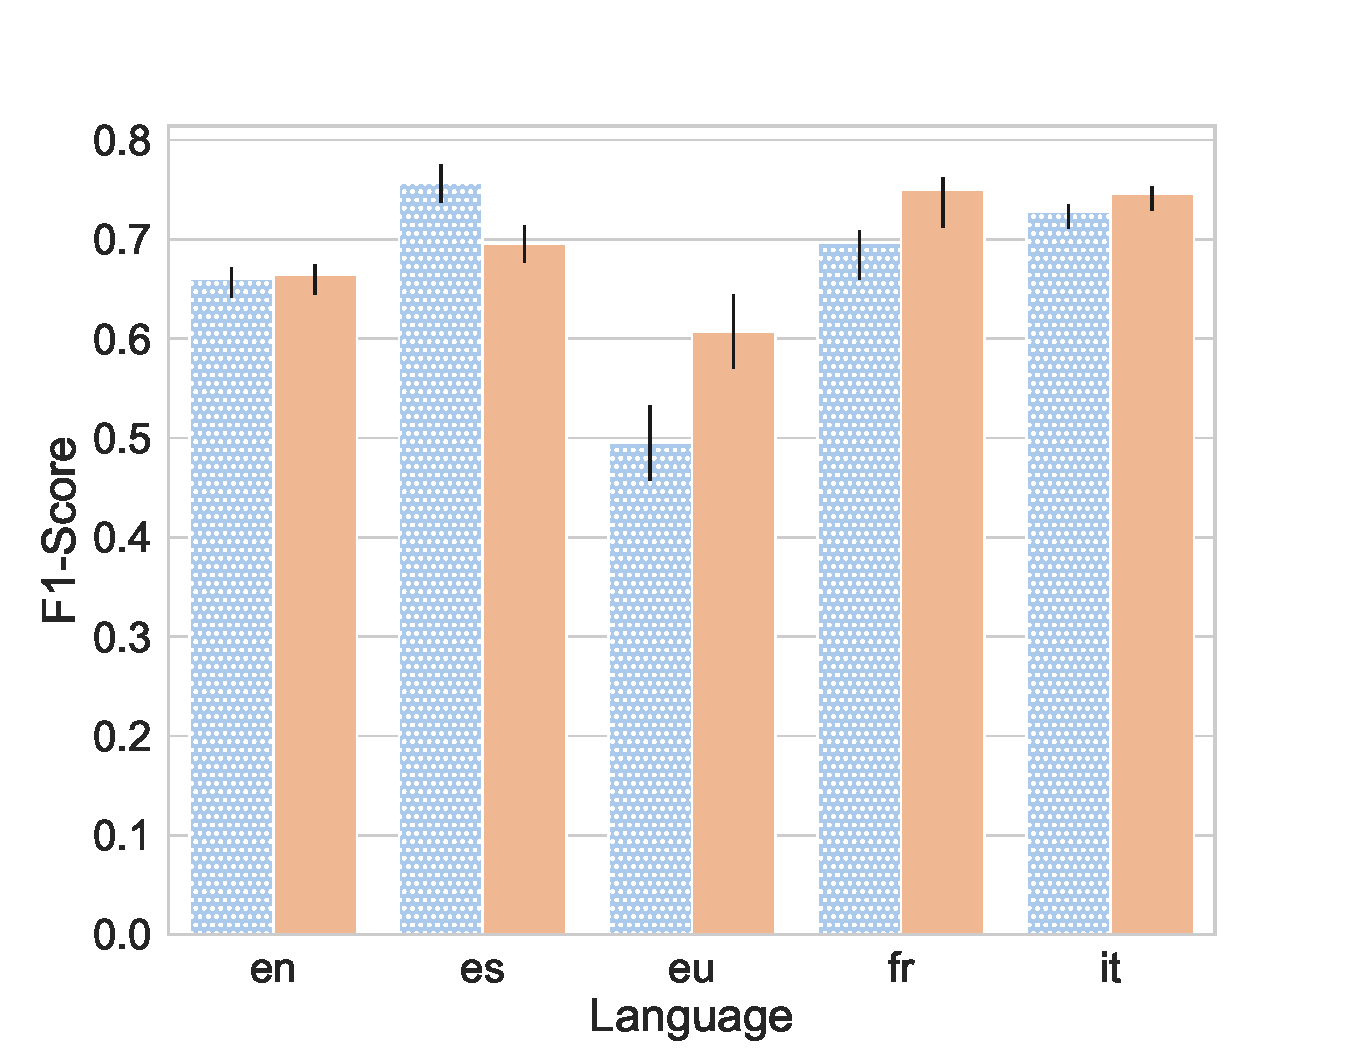
\includegraphics[width=0.5\textwidth]{figures/multi_weak_supervision/plot_A.pdf}
    \caption{A graph with the mean F1-score of the models on the y-axis and the different language on the x-axis for the \SettingA. The orange bar represents the \distilmodels F1-Scores whereas the dotted blue bars represent the \weakModel F1-score.}
    % describe figure
    \label{fig:setting_A}
\end{figure}

\paragraph{\SettingB} The amount of annotated tokens in {\layerValidate} is relatively small compared to \layerTwo(Figure \ref{tab:counts}). 
This hurts the result (Table \ref{tab:global}) of the \distilmodels ($0.61$ with {\layerValidate} vs $0.70$ with \layerTwo) in contrast to the {\weakModel}, where performance has gained $0.03$ ($0.70$ with {\layerValidate} vs $0.67$ with \layerTwo). The {\weakModel} performance is relatively better than the \distilmodels. Moreover, the \distilmodels recall performance seems to be affected by the small amount of data and annotated tokens ($0.68$ for \SettingD $with$ $r=1$  vs $0.58$ for \SettingB $with$ $r=1$).  
\paragraph{\SettingC} The results (Table \ref{tab:global}) show better performance for both models when we mix a slight quantity of manually annotated data with \layerTwo. The \distilmodels outperforms the \weakModel with a gain of $0.03$. In both cases, the F1-Score gain is due to the improvement of the recall: we obtain a gain of $0.05$ compared to the \SettingA.
\paragraph{\SettingD} For all languages except Basque, we obtained better results when we mixed weak supervised and {\instruct} annotations. The local optimum for these languages is reached when $r \in [0.4, 0.6]$ (Figure \ref{fig:confuse}). The Basque doesn't follow this trend; using a dataset with only {\instruct} annotations (where $r = 1$) gives the best result among all tried $r$ values.
\paragraph{\SettingE} Using a multilingual train set and LM (\verb|xlm-roberta-base|) gives inferior results compared to \SettingD (Table \ref{tab:global_d}). Though we obtain better results in Italian than the \SettingD ($+ 0.01$); the optimum is set to $r = 0.8$. In the other case, mixing annotations described in \ref{sec:prot} don't affect results as observed in \SettingD due to the noise generated by the multilingual nature of the train set. 

\begin{figure}[t!]
    \begin{subfigure}[t]{0.5\textwidth}
        \centering
        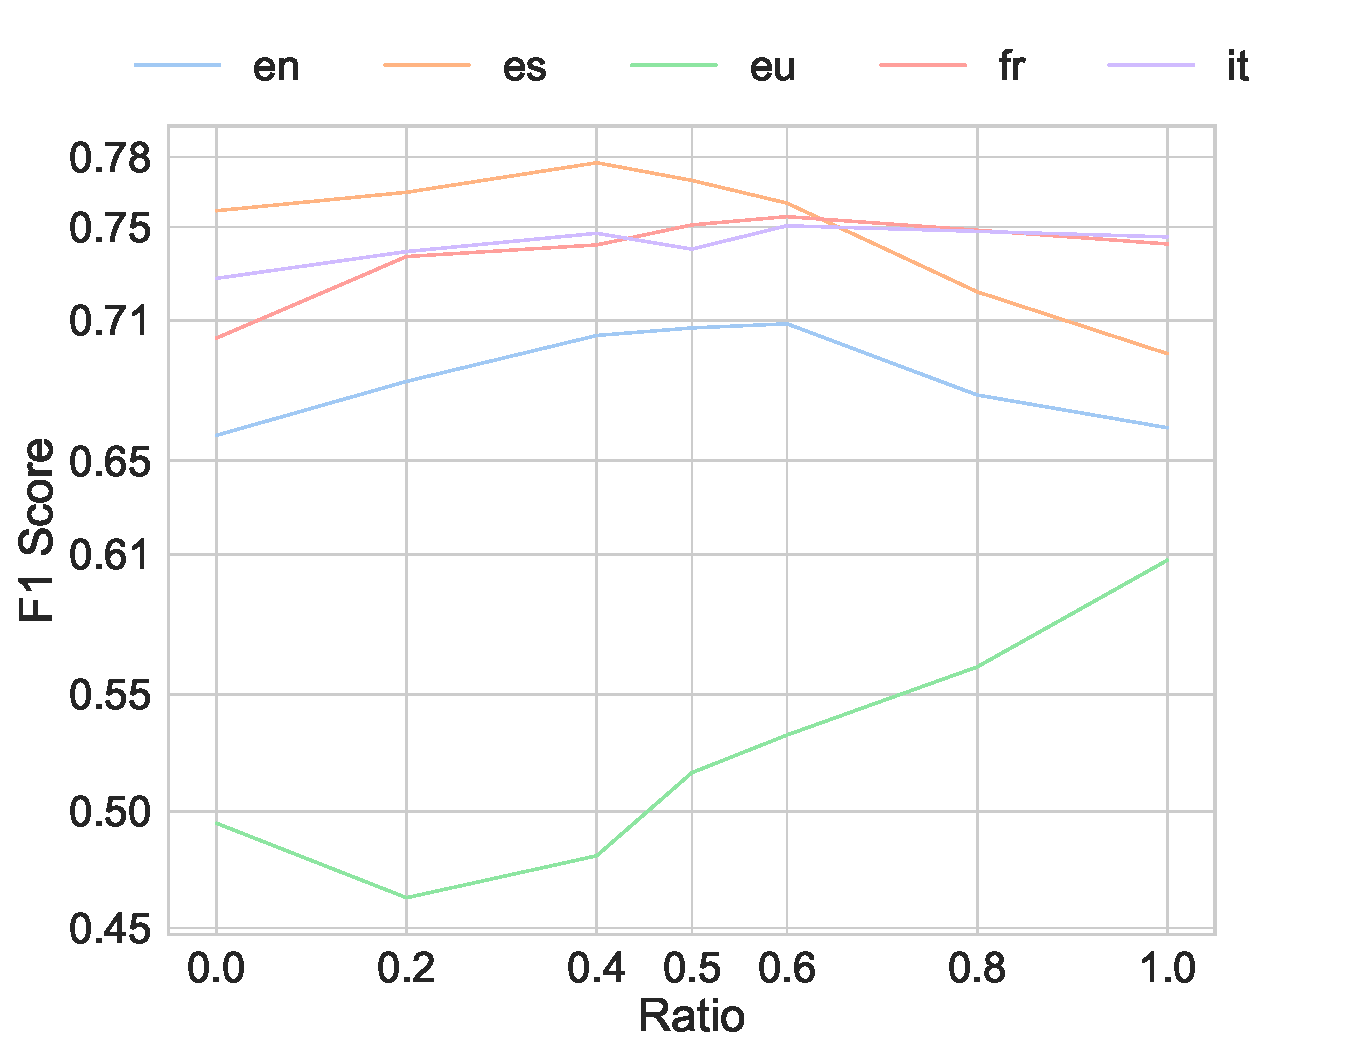
\includegraphics[height=2.3in]{figures/multi_weak_supervision/conf_D.pdf}
        \caption{\SettingD}
    \end{subfigure}
    \begin{subfigure}[t]{0.5\textwidth}
        \centering
        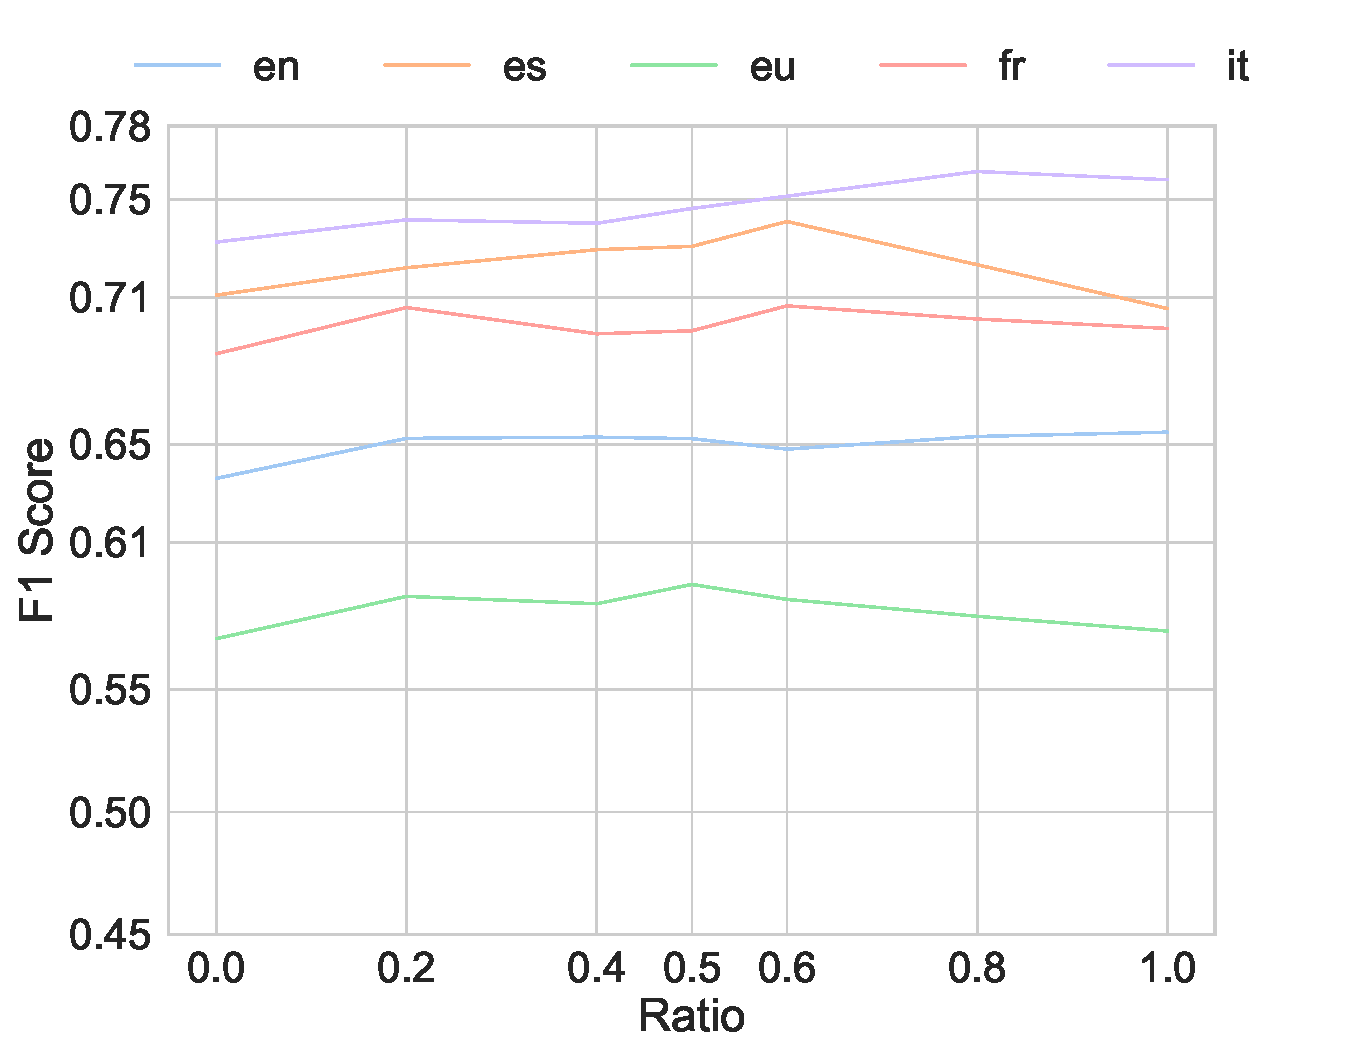
\includegraphics[height=2.3in]{figures/multi_weak_supervision/conf_E.pdf}
        \caption{\SettingE}
    \end{subfigure}
    \caption{The line plots with the mean F1-score of the models on the y-axis and the ratio of dictionary annotations and annotations via InstructGPT-3 on the x-axis for \SettingD and \SettingE as described in \ref{sec:prot}. A ratio of $r=0$ indicates the presence of only dictionary annotations, while a ratio of $r=1$ corresponds to exclusively InstructGPT-3 annotations. Each coloured line represents the result for a language }
    \label{fig:confuse}
\end{figure}

\begin{table*}
    \centering
    \small
    \resizebox{1\textwidth}{!}{
        \begin{tabular}{@{}ccccccc@{}}%
\toprule%
Setting&\multicolumn{2}{c}{F1-Score}&\multicolumn{2}{c}{Precision}&\multicolumn{2}{c}{Recall}\\%
&$r=1$&$r=0$&$r=1$&$r=0$&$r=1$&$r=0$\\%
\midrule%
\SettingD&\textbf{0.70} \bm{$\pm$} \textbf{0.06}&0.67  $\pm$ 0.09&0.73  $\pm$ 0.03&\textbf{0.78} \bm{$\pm$} \textbf{0.09}&\textbf{0.68} \bm{$\pm$} \textbf{0.09}&0.63  $\pm$ 0.10\\%
\SettingB&0.61  $\pm$ 0.09&\textbf{0.70} \bm{$\pm$} \textbf{0.06}&0.72  $\pm$ 0.03&\textbf{0.75} \bm{$\pm$} \textbf{0.04}&0.58  $\pm$ 0.10&\textbf{0.69} \bm{$\pm$} \textbf{0.05}\\%
\SettingC&\textbf{0.73} \bm{$\pm$} \textbf{0.03}&0.71  $\pm$ 0.08&0.74  $\pm$ 0.04&\textbf{0.78} \bm{$\pm$} \textbf{0.05}&\textbf{0.73} \bm{$\pm$} \textbf{0.06}&0.68  $\pm$ 0.08\\\bottomrule%
%
\end{tabular}
    }
    \caption{The F1-score, Precision and the Recall for the different settings in section \ref{sec:prot}. $r=1$ corresponds to the \distilmodels and the $r=0$ corresponds to the \weakModel.}
    \label{tab:global}
\end{table*}
\begin{table}
    \centering
    \small
    \resizebox{1\columnwidth}{!}{
        \begin{tabular}{@{}cccc@{}}%
\toprule%
Setting&\multicolumn{1}{c}{F1-Score}&\multicolumn{1}{c}{Precision}&\multicolumn{1}{c}{Recall}\\%
&$\rmix_{max}$&$\rmix_{max}$&$\rmix_{max}$\\%
\midrule%
\Ssilver&\textbf{0.72} \bm{$\pm$} \textbf{0.06}&0.75 $\pm$ 0.02&\textbf{0.71} \bm{$\pm$} \textbf{0.08}\\%
\Smulti&0.69 $\pm$ 0.06&\textbf{0.79} \bm{$\pm$} \textbf{0.03}&0.65 $\pm$ 0.08\\\bottomrule%
%
\end{tabular}
    }
    \caption{The F1-score, Precision, and Recall for \SettingD and \SettingE as described in Section~\ref{sec:prot}. The scores are aggregated across languages, with $r_{max}$ representing the optimal value of $r$.}
    \label{tab:global_d}
\end{table}
\subsection{Discussion}

Our experiments using the E3C dataset demonstrate the potential of knowledge distillation and weak supervision in the context of clinical entity extraction tasks. We observe that distilled models outperform classic weak supervision approaches, especially in Basque, French, and Italian languages. However, we notice some interesting trends in English and Spanish that require further analysis.

The trend is reversed in Spanish, with the \weakModel~ performing better than the distilled ones. For all the models we trained for Spanish (Table \ref{tab:models}), we don't distinguish any difference between monolingual, agnostic domain, multilingual, or medical monolingual language models.
One possible explanation for these trends is the difference in data sources. While the corpora for other languages come from the Pan African Journal or Pubmed, the Spanish corpus is sourced from the SPACCC corpus. The clinical entity distribution and semantic differences from this source could bias our results. Moreover, additional data cleaning has been applied to layer 1, such as sentence and punctuation removal and capitalization, which may reinforce this difference between the languages.

In English, the difference in performance between distilled and weak-supervised models is relatively small compared to other languages. This can be attributed to the superior quality of annotations in the \layerTwo. The English lexicon resource (supplied by the UMLS meta-thesaurus and terms extracted in \layerOne) employed for mapping clinical entities in the text is likely more extensive and precise than those accessible for other languages with fewer linguistic resources.

Furthermore, \SettingD reveals that combining annotations from Dictionary extraction and \instruct marginally outperforms when \mbox{$r=1$}. Integrating various annotation sources shows promise and typically enhances model generalization. However, in the case of Basque, \SettingD does not yield the best results when we have only \instruct annotations (\mbox{$r=1$}). As we raise the ratio $r$, we observe a gradual improvement in F1-score. It can be explained by the original annotations from \layerTwo in Basque was created using a low-resource lexicon. As shown in Table \ref{tab:counts}, only 63 \iclin tokens were initially annotated, in contrast to 482 tokens for \instruct annotations.

In the case of \SettingE, we did not observe any significant results. The performance of Spanish, Italian, and French languages either experienced a slight improvement or was unaffected by the multilingual composition of the training dataset. However, this setting negatively impacted English and Basque. The predominance of Romance languages in the dataset could be the cause.

Moreover, Basque is a distinct and isolated language with unique linguistic structures. The other languages in the training dataset are linguistically distant, which may introduce noise during the training process and consequently affect the performance of the Basque model.

Another interesting observation is that \instruct extracts almost twice as many entities as the original extraction method (Figure \ref{tab:counts}). This trend is more pronounced in \layerTwo, while the number of annotated tokens in \layerValidate is almost equivalent between both annotation sets, likely due to human validation. This difference could be explained by the fact that \instruct has no access to the guidelines, and the prompt mentioned to extract "disorders," "disease," or "symptoms" is less restrictive than the E3C guideline annotation.

Our results highlight the potential of knowledge distillation and weak supervision for clinical entity extraction, particularly for languages with more limited resources. Though, data sources, annotation quality, and the comprehensiveness of linguistic resources influence the performance of these methods. 
Further research is needed to address these challenges and improve our methods.

\section{Limitation}
One limitation of our study is the small size of the test set, which may impact the generalizability of our results. Additionally, we restrained our work on clinical entity extraction; in future work, we would investigate more in several tasks using the E3C temporality layer to cover a task of Name Entity Recognition and Relation Extraction tasks.

Finally, the E3C guidelines have been designed for clinical entity extraction and entity-linking via UMLS entities. After the first step of manual annotation, some spans of the entities have been modified to fit as close as possible to the semantical concepts found in UMLS \citep{Magnini2020TheCases}. For instance, clinical entities could be split into separate disorder concepts, and the extent of a disorder candidate could be reduced to fit with a concept. These biases could induce additional difficulties in finding the correct span for a given model.

\section{Conclusion}
Our results demonstrate that the knowledge distillation with \instruct outperforms the dictionary supervision for extracting clinical entities. 

We show that mixing these approaches to build a training dataset brings diversity to the annotations and improves the distilled model performance.

Weak-supervision approach with LLMs is relatively promising for creating a training dataset. This reduces the annotation cost and, at the same time, focuses the manual annotation on the test set, which is one of the most prominent parts of high-stake domains like healthcare. Furthermore, the interest of the approach is also to fine-tune a small to medium-sized LM that may be used locally without the leak of confidential medical data and with a reduced energy cost.
In a low-resource context, such as Basque, LLMs offer a competitive alternative to the classic weak supervision technique, which requires linguistic resources. 

Furthermore, we aim to investigate advanced techniques to combine various annotations by incorporating confidence measures from the different predictions. Using other LLMs predictions and ensemble, the difference could be pertinent because the annotation diversity can improve a model's performance, as we observed on \SettingD (Figure \ref{fig:confuse}).  
Additionally, we will consider utilising performance metrics (such as recall and precision) to decide which type of annotations (begin or inner-tokens) to retain for each prediction method.

Finally, adapting CoT or generated knowledge \citep{Wei2022ChainModels, Cobbe2021TrainingProblems} for clinical entity extraction could improve LLM's precision.
To our knowledge, none of these techniques has been adapted to clinical information retrieval. We could craft a prompt with different annotation steps through different examples. At each annotation step, we describe a precise instruction and its result. For example, incorporating the three steps of the E3C annotation into the prompt could help encourage the LLM to better adhere to the guideline.

\section{Additional Material}
\label{section:app}
\definecolor{mint}{RGB}{209,227,221}
\definecolor{savoyblue}{RGB}{176,109,53}
\definecolor{glaucous}{RGB}{110,125,171}
\definecolor{pink}{RGB}{147,93,154}
\begin{figure}[h!]
\begin{Verbatim}[frame=single,fontsize=\scriptsize,commandchars=\\\{\}]
\colorbox{glaucous}{\color{white}{Input:  The evolution was marked two months later,}}
\colorbox{glaucous}{\color{white}{by the appearance of angiomatous plaques on the}} 
\colorbox{glaucous}{\color{white}{right forearm, [...]}} 
\colorbox{glaucous}{\color{white}{extract the exact match of disorders, diseases or}} 
\colorbox{glaucous}{\color{white}{symptoms mentioned in the text or}} 
\colorbox{glaucous}{\color{white}{return None if there is no clinical entity:}}

\colorbox{glaucous}{\color{white}{- "angiomatous plaques"}}
\colorbox{glaucous}{\color{white}{- "lymphedema"}}
\colorbox{glaucous}{\color{white}{- "lesions"}}

\colorbox{glaucous}{\color{white}{Input:  At the same time, the patient had presented}} 
\colorbox{glaucous}{\color{white}{a progressive alteration of the general condition,}} 
\colorbox{glaucous}{\color{white}{a fever and night sweats}}
\colorbox{glaucous}{\color{white}{extract the exact match of disorders, diseases}} 
\colorbox{glaucous}{\color{white}{or symptoms mentioned in the text or}} 
\colorbox{glaucous}{\color{white}{return None if there is no clinical entity:}}

\colorbox{glaucous}{\color{white}{- "progressive alteration of the general condition"}}
\colorbox{glaucous}{\color{white}{- "fever"}}
\colorbox{glaucous}{\color{white}{- "night sweats"}}

\colorbox{glaucous}{\color{white}{Input:  The sedimentation rate was 35mm at the}} 
\colorbox{glaucous}{\color{white}{first hour, C-reactive protein was negative}} 
\colorbox{glaucous}{\color{white}{and ferritin level was 900µg/l}} 
\colorbox{glaucous}{\color{white}{(i.e., 4 times the normal value).}}
\colorbox{glaucous}{\color{white}{extract the exact match of disorders, diseases}} 
\colorbox{glaucous}{\color{white}{or symptoms mentioned in the text or}} 
\colorbox{glaucous}{\color{white}{return None if there is no clinical entity:}}

\colorbox{glaucous}{\color{white}{- "None"}}

\colorbox{savoyblue}{\color{white}{Input:  The interview revealed no history}} 
\colorbox{savoyblue}{\color{white}{of any pathological events, in particular}} 
\colorbox{savoyblue}{\color{white}{skin rash, gastrointestinal disorders, jaundice,}} 
\colorbox{savoyblue}{\color{white}{respiratory infection or recent vaccination.}}
\colorbox{pink}{\color{white}{extract the exact match of disorders, diseases}}
\colorbox{pink}{\color{white}{or symptoms mentioned in the text or}}
\colorbox{pink}{\color{white}{return None if there is no clinical entity:}}
\colorbox{mint}{\color{white}{- "}}

\end{Verbatim}
\caption{An example of the prompt used in our experiment. The formatted examples are shown in \colorbox{glaucous}{\color{white}{blue}}, while the formatted examples to predict are shown in \colorbox{savoyblue}{\color{white}{orange}}. The instructions are shown in \colorbox{pink}{\color{white}{purple}}, and the guidance, as used in \citet{Agrawal2022LargeExtractors}, is shown in \colorbox{mint}{\color{white}{green}}. For all languages, instruction is still in English, but the formatted examples are in the source language.}
\label{fig:prompt}
\end{figure}


\begin{table*}
    \centering
    \small
    \resizebox{1\textwidth}{!}{
        \begin{tabular}{@{}cccc@{}}%
\toprule%
Language&Model&\multicolumn{2}{c}{F1-Score}\\%
&&$r=1$&$r=0$\\%
\midrule%
en&\verb|emilyalsentzer/Bio_ClinicalBERT|&0.66  $\pm$ 0.01&\textbf{0.68} \bm{$\pm$} \textbf{0.01}\\%
&\verb|roberta-base|&\textbf{0.67} \bm{$\pm$} \textbf{0.01}&0.65  $\pm$ 0.01\\%
&\verb|xlm-roberta-base|&\textbf{0.66} \bm{$\pm$} \textbf{0.01}&0.65  $\pm$ 0.01\\%
\midrule%
es&\verb|BSC-LT/roberta-base-biomedical-es|&0.72  $\pm$ 0.01&\textbf{0.78} \bm{$\pm$} \textbf{0.01}\\%
&\verb|dccuchile/bert-base-spanish-wwm-cased|&0.69  $\pm$ 0.01&\textbf{0.76} \bm{$\pm$} \textbf{0.01}\\%
&\verb|xlm-roberta-base|&0.68  $\pm$ 0.02&\textbf{0.73} \bm{$\pm$} \textbf{0.01}\\%
\midrule%
eu&\verb|ixa-ehu/berteus-base-cased|&\textbf{0.60} \bm{$\pm$} \textbf{0.03}&0.54  $\pm$ 0.03\\%
&\verb|xlm-roberta-base|&\textbf{0.61} \bm{$\pm$} \textbf{0.04}&0.47  $\pm$ 0.01\\%
\midrule%
fr&\verb|Dr-BERT/DrBERT-7GB|&\textbf{0.74} \bm{$\pm$} \textbf{0.01}&0.70  $\pm$ 0.01\\%
&\verb|camembert-base|&\textbf{0.75} \bm{$\pm$} \textbf{0.01}&0.69  $\pm$ 0.04\\%
&\verb|xlm-roberta-base|&\textbf{0.74} \bm{$\pm$} \textbf{0.01}&0.72  $\pm$ 0.02\\%
\midrule%
it&\verb|dbmdz/bert-base-italian-cased|&\textbf{0.74} \bm{$\pm$} \textbf{0.01}&0.73  $\pm$ 0.00\\%
&\verb|xlm-roberta-base|&\textbf{0.75} \bm{$\pm$} \textbf{0.01}&0.72  $\pm$ 0.02\\\bottomrule%
%
\end{tabular}
    }
    \caption{This table reports the F1-Scores for the different models and annotation ratios $r \in \{0,1\}$ for \SettingD described in Section~\ref{sec:prot}.}
\end{table*}

\begin{table*}
    \centering
    \small
    \resizebox{1\textwidth}{!}{
        \begin{tabular}{@{}cccc@{}}%
\toprule%
Language&Model&\multicolumn{2}{c}{F1-Score}\\%
&&$\rmix=1$&$\rmix=0$\\%
\midrule%
en&\verb|emilyalsentzer/Bio_ClinicalBERT|&0.60&\textbf{0.65}\\%
&\verb|roberta-base|&0.61&\textbf{0.70}\\%
&\verb|xlm-roberta-base|&0.43&\textbf{0.69}\\%
\midrule%
es&\verb|BSC-LT/roberta-base-biomedical-es|&0.71&\textbf{0.78}\\%
&\verb|dccuchile/bert-base-spanish-wwm-cased|&0.70&\textbf{0.77}\\%
&\verb|xlm-roberta-base|&0.62&\textbf{0.73}\\%
\midrule%
eu&\verb|ixa-ehu/berteus-base-cased|&0.54&\textbf{0.72}\\%
&\verb|xlm-roberta-base|&0.51&\textbf{0.68}\\%
\midrule%
fr&\verb|Dr-BERT/DrBERT-7GB|&0.73&\textbf{0.75}\\%
&\verb|camembert-base|&\textbf{0.71}&0.60\\%
&\verb|xlm-roberta-base|&0.68&\textbf{0.68}\\%
\midrule%
it&\verb|dbmdz/bert-base-italian-cased|&0.63&\textbf{0.70}\\%
&\verb|xlm-roberta-base|&0.55&\textbf{0.57}\\\bottomrule%
%
\end{tabular}
    }
    \caption{This table reports the F1-Scores for the different models and annotation ratios $r \in \{0,1\}$ for \SettingB described in Section~\ref{sec:prot}.}
\end{table*}

\begin{table*}
    \centering
    \small
    \resizebox{1\textwidth}{!}{
        \begin{tabular}{@{}cccc@{}}%
\toprule%
Language&Model&\multicolumn{2}{c}{F1-Score}\\%
&&$\rmix=1$&$\rmix=0$\\%
\midrule%
en&\verb|emilyalsentzer/Bio_ClinicalBERT|&\textbf{0.70} \bm{$\pm$} \textbf{0.01}&0.69  $\pm$ 0.01\\%
&\verb|roberta-base|&\textbf{0.70} \bm{$\pm$} \textbf{0.01}&0.68  $\pm$ 0.01\\%
&\verb|xlm-roberta-base|&\textbf{0.67} \bm{$\pm$} \textbf{0.01}&0.67  $\pm$ 0.01\\%
\midrule%
es&\verb|BSC-LT/roberta-base-biomedical-es|&0.77  $\pm$ 0.02&\textbf{0.80} \bm{$\pm$} \textbf{0.01}\\%
&\verb|dccuchile/bert-base-spanish-wwm-cased|&0.76  $\pm$ 0.01&\textbf{0.78} \bm{$\pm$} \textbf{0.00}\\%
&\verb|xlm-roberta-base|&0.76  $\pm$ 0.01&\textbf{0.76} \bm{$\pm$} \textbf{0.01}\\%
\midrule%
eu&\verb|ixa-ehu/berteus-base-cased|&0.70  $\pm$ 0.03&\textbf{0.72} \bm{$\pm$} \textbf{0.02}\\%
&\verb|xlm-roberta-base|&\textbf{0.70} \bm{$\pm$} \textbf{0.01}&0.57  $\pm$ 0.09\\%
\midrule%
fr&\verb|Dr-BERT/DrBERT-7GB|&\textbf{0.75} \bm{$\pm$} \textbf{0.01}&0.73  $\pm$ 0.02\\%
&\verb|camembert-base|&\textbf{0.76} \bm{$\pm$} \textbf{0.01}&0.74  $\pm$ 0.01\\%
&\verb|xlm-roberta-base|&\textbf{0.74} \bm{$\pm$} \textbf{0.01}&0.69  $\pm$ 0.04\\%
\midrule%
it&\verb|dbmdz/bert-base-italian-cased|&\textbf{0.75} \bm{$\pm$} \textbf{0.01}&0.75  $\pm$ 0.01\\%
&\verb|xlm-roberta-base|&\textbf{0.74} \bm{$\pm$} \textbf{0.00}&0.74  $\pm$ 0.01\\\bottomrule%
%
\end{tabular}
    }
    \caption{This table reports F1-Scores for different models and annotation ratios $r \in \{0,1\}$ for \SettingC described in Section~\ref{sec:prot}.}
\end{table*}

\begin{table*}
    \centering
    \resizebox{1\textwidth}{!}{
        \begin{tabular}{@{}cccccccccccc@{}}%
\toprule%
Language&Model&$r_{max}$&\multicolumn{3}{c}{$r=1$}&\multicolumn{3}{c}{$r_{max}$}&\multicolumn{3}{c}{$r=0$}\\%
&&&F1-Score&Precision&Recall&F1-Score&Precision&Recall&F1-Score&Precision&Recall\\%
\midrule%
en&\verb|xlm-roberta-base|&0.5&0.65 \bm{$\pm$} 0.01&0.72 \bm{$\pm$} 0.01&0.63 \bm{$\pm$} 0.01&0.71 \bm{$\pm$} 0.01&0.71 \bm{$\pm$} 0.03&0.71 \bm{$\pm$} 0.02&0.66 \bm{$\pm$} 0.01&0.68 \bm{$\pm$} 0.03&0.64 \bm{$\pm$} 0.02\\%
&\verb|roberta-base|&0.4&0.65 \bm{$\pm$} 0.01&0.72 \bm{$\pm$} 0.01&0.62 \bm{$\pm$} 0.02&0.71 \bm{$\pm$} 0.01&0.72 \bm{$\pm$} 0.01&0.71 \bm{$\pm$} 0.03&0.67 \bm{$\pm$} 0.01&0.70 \bm{$\pm$} 0.01&0.65 \bm{$\pm$} 0.01\\%
&\verb|emilyalsentzer/Bio_ClinicalBERT|&0.6&0.68 \bm{$\pm$} 0.01&0.73 \bm{$\pm$} 0.01&0.66 \bm{$\pm$} 0.02&0.72 \bm{$\pm$} 0.01&0.75 \bm{$\pm$} 0.02&0.70 \bm{$\pm$} 0.02&0.66 \bm{$\pm$} 0.01&0.71 \bm{$\pm$} 0.02&0.63 \bm{$\pm$} 0.01\\%
\midrule%
es&\verb|xlm-roberta-base|&0.4&0.73 \bm{$\pm$} 0.01&0.80 \bm{$\pm$} 0.01&0.70 \bm{$\pm$} 0.01&0.76 \bm{$\pm$} 0.01&0.77 \bm{$\pm$} 0.02&0.76 \bm{$\pm$} 0.02&0.68 \bm{$\pm$} 0.02&0.74 \bm{$\pm$} 0.02&0.65 \bm{$\pm$} 0.04\\%
&\verb|dccuchile/bert-base-spanish-wwm-cased|&0.4&0.76 \bm{$\pm$} 0.01&0.81 \bm{$\pm$} 0.01&0.73 \bm{$\pm$} 0.02&0.78 \bm{$\pm$} 0.00&0.80 \bm{$\pm$} 0.02&0.76 \bm{$\pm$} 0.02&0.69 \bm{$\pm$} 0.01&0.72 \bm{$\pm$} 0.02&0.66 \bm{$\pm$} 0.03\\%
&\verb|BSC-LT/roberta-base-biomedical-es|&0.4&0.78 \bm{$\pm$} 0.01&0.82 \bm{$\pm$} 0.01&0.75 \bm{$\pm$} 0.01&0.79 \bm{$\pm$} 0.01&0.80 \bm{$\pm$} 0.04&0.79 \bm{$\pm$} 0.03&0.72 \bm{$\pm$} 0.01&0.75 \bm{$\pm$} 0.02&0.69 \bm{$\pm$} 0.02\\%
\midrule%
eu&\verb|xlm-roberta-base|&1&0.47 \bm{$\pm$} 0.01&0.63 \bm{$\pm$} 0.14&0.44 \bm{$\pm$} 0.01&{-}&{-}&{-}&0.61 \bm{$\pm$} 0.04&0.73 \bm{$\pm$} 0.02&0.56 \bm{$\pm$} 0.05\\%
&\verb|ixa-ehu/berteus-base-cased|&1&0.54 \bm{$\pm$} 0.03&0.91 \bm{$\pm$} 0.01&0.49 \bm{$\pm$} 0.02&{-}&{-}&{-}&0.60 \bm{$\pm$} 0.03&0.74 \bm{$\pm$} 0.02&0.54 \bm{$\pm$} 0.03\\%
\midrule%
fr&\verb|xlm-roberta-base|&0.4&0.72 \bm{$\pm$} 0.02&0.80 \bm{$\pm$} 0.02&0.67 \bm{$\pm$} 0.03&0.75 \bm{$\pm$} 0.01&0.75 \bm{$\pm$} 0.02&0.75 \bm{$\pm$} 0.02&0.74 \bm{$\pm$} 0.01&0.74 \bm{$\pm$} 0.02&0.74 \bm{$\pm$} 0.02\\%
&\verb|camembert-base|&0.5&0.74 \bm{$\pm$} 0.01&0.69 \bm{$\pm$} 0.01&0.83 \bm{$\pm$} 0.01&0.76 \bm{$\pm$} 0.01&0.73 \bm{$\pm$} 0.02&0.81 \bm{$\pm$} 0.03&0.75 \bm{$\pm$} 0.00&0.82 \bm{$\pm$} 0.01&0.71 \bm{$\pm$} 0.01\\%
&\verb|Dr-BERT/DrBERT-7GB|&0.6&0.70 \bm{$\pm$} 0.01&0.84 \bm{$\pm$} 0.00&0.64 \bm{$\pm$} 0.01&0.76 \bm{$\pm$} 0.01&0.76 \bm{$\pm$} 0.01&0.77 \bm{$\pm$} 0.01&0.74 \bm{$\pm$} 0.01&0.77 \bm{$\pm$} 0.04&0.73 \bm{$\pm$} 0.04\\%
\midrule%
it&\verb|xlm-roberta-base|&0.6&0.72 \bm{$\pm$} 0.02&0.78 \bm{$\pm$} 0.02&0.70 \bm{$\pm$} 0.04&0.75 \bm{$\pm$} 0.02&0.76 \bm{$\pm$} 0.02&0.76 \bm{$\pm$} 0.02&0.75 \bm{$\pm$} 0.01&0.75 \bm{$\pm$} 0.02&0.75 \bm{$\pm$} 0.02\\%
&\verb|dbmdz/bert-base-italian-cased|&0.8&0.73 \bm{$\pm$} 0.00&0.76 \bm{$\pm$} 0.02&0.73 \bm{$\pm$} 0.02&0.75 \bm{$\pm$} 0.00&0.72 \bm{$\pm$} 0.02&0.81 \bm{$\pm$} 0.02&0.74 \bm{$\pm$} 0.01&0.70 \bm{$\pm$} 0.02&0.81 \bm{$\pm$} 0.02\\\bottomrule%
%
\end{tabular}
    }
        \caption{This table presents F1-Scores, Precision, and Recall for different models at annotation ratios $r \in \{0,1\}$ and at the optimal $r$ value, $r_{max}$ for \SettingD, as described in Section~\ref{sec:prot}.}
\end{table*}

\begin{table*}
    \centering
    \resizebox{1\textwidth}{!}{
        \begin{tabular}{@{}cccccc@{}}%
\toprule%
Language&$\rmix_{max}$&Metric&{$\rmix=1$}&{$\rmix_{max}$}&{$\rmix=0$}\\%
\midrule%
\multirow{3}{*}{en}&\multirow{3}{*}{1}&F1-Score&0.64 \bm{$\pm$} 0.01&{-}&0.66 \bm{$\pm$} 0.03\\%
&&Precision&0.74 \bm{$\pm$} 0.01&{-}&0.75 \bm{$\pm$} 0.03\\%
&&Recall&0.60 \bm{$\pm$} 0.01&{-}&0.62 \bm{$\pm$} 0.05\\%
\midrule%
\multirow{3}{*}{es}&\multirow{3}{*}{0.6}&F1-Score&0.71 \bm{$\pm$} 0.01&0.74 \bm{$\pm$} 0.01&0.71 \bm{$\pm$} 0.01\\%
&&Precision&0.82 \bm{$\pm$} 0.01&0.83 \bm{$\pm$} 0.02&0.80 \bm{$\pm$} 0.03\\%
&&Recall&0.65 \bm{$\pm$} 0.02&0.69 \bm{$\pm$} 0.02&0.65 \bm{$\pm$} 0.02\\%
\midrule%
\multirow{3}{*}{eu}&\multirow{3}{*}{0.5}&F1-Score&0.57 \bm{$\pm$} 0.02&0.59 \bm{$\pm$} 0.02&0.57 \bm{$\pm$} 0.01\\%
&&Precision&0.86 \bm{$\pm$} 0.02&0.79 \bm{$\pm$} 0.02&0.76 \bm{$\pm$} 0.04\\%
&&Recall&0.51 \bm{$\pm$} 0.02&0.54 \bm{$\pm$} 0.02&0.51 \bm{$\pm$} 0.01\\%
\midrule%
\multirow{3}{*}{fr}&\multirow{3}{*}{0.6}&F1-Score&0.69 \bm{$\pm$} 0.02&0.71 \bm{$\pm$} 0.01&0.70 \bm{$\pm$} 0.02\\%
&&Precision&0.83 \bm{$\pm$} 0.01&0.81 \bm{$\pm$} 0.02&0.80 \bm{$\pm$} 0.02\\%
&&Recall&0.62 \bm{$\pm$} 0.02&0.65 \bm{$\pm$} 0.02&0.64 \bm{$\pm$} 0.03\\%
\midrule%
\multirow{3}{*}{it}&\multirow{3}{*}{0.8}&F1-Score&0.73 \bm{$\pm$} 0.01&0.76 \bm{$\pm$} 0.01&0.76 \bm{$\pm$} 0.01\\%
&&Precision&0.78 \bm{$\pm$} 0.01&0.76 \bm{$\pm$} 0.01&0.75 \bm{$\pm$} 0.03\\%
&&Recall&0.71 \bm{$\pm$} 0.01&0.77 \bm{$\pm$} 0.02&0.78 \bm{$\pm$} 0.02\\\bottomrule%
%
\end{tabular}

    }
    \caption{This tabie presents F1-Scores, Precision, and Recall for different models at annotation ratios $r \in \{0,1\}$ and at the optimal $r$ value, $r_{max}$ for \SettingE, as described in Section~\ref{sec:prot}.}
\end{table*}

\chapter{Improvements and Extensions of the Synthetic Generation Pipeline}
\label{chap:evaluation}

Having demonstrated the viability of our privacy-safe synthetic document generation approach on MIMIC-III through ICD-9 classification and NER tasks, we identified several opportunities to extend and refine our methodology. The previous chapter established that our keyword-guided generation coupled with reward-based refinement successfully produces high-quality synthetic documents that can match or exceed the performance of models trained on real data. However, the evaluation remained constrained to specific task types and datasets, and several limitations emerged regarding task complexity, evaluation robustness, and privacy guarantees.

This chapter explores three key extensions to address these limitations and broaden the applicability of our approach. First, we extend our evaluation to more complex conversational medical tasks using the AlpaCare benchmark, enabling direct comparison with related privacy-preserving methods like KnowledgeSG. Second, we investigate advanced filtering and evaluation techniques—including medical domain filtering and LLM-as-judge mechanisms—to improve the quality of synthetic document selection beyond the SemScore metric employed in our initial pipeline. Third, we conduct rigorous privacy analysis through linkage and discrimination attacks to quantify re-identification risks and validate the privacy guarantees of our generated documents.

To support these investigations, we build upon our core synthetic generation pipeline, which addresses the critical need for producing high-quality training data while preserving patient information confidentiality. The approach relies on decoder-type generative models (we use Llama2-7B \cite{touvron2023llama} and Mistral-7B \cite{jiang2023mistral} in our experiments) coupled with an iterative reinforcement improvement process, guided by feedback signals from evaluator models that compare generated documents to public and private reference corpora. The pipeline is structured around five main phases: (1) clinical entity keyword extraction using QuickUMLS \cite{soldaini2016quickumls} to ensure no direct patient identification; (2) supervised fine-tuning on pseudo-anonymized or differentially private documents; (3) candidate document generation; (4) evaluation by scorer models quantifying semantic quality; and (5) alignment through reinforcement learning using DPO \cite{rafailov2023dpo} or KTO \cite{ethayarajh2024kto} for continuous improvement.

\minitoc

\section{Extension of evaluation benchmarks}
Since our method shares several conceptual similarities with KnowledgeSG \cite{knowledgesg2024}, we sought to establish a comparison with this approach. KnowledgeSG proposes a client-server framework where the client possesses private knowledge (for example, a clinical model trained on sensitive data) while a knowledge distillation process occurs via a remote professional model. Like our pipeline, this method adopts an iterative approach and integrates alignment mechanisms and sample selection: it generates multiple candidates then progressively filters them via a reference professional model to select the best samples, thus countering the performance degradation induced by gradient noise when using differential privacy.

This methodological convergence naturally led us to adopt the AlpaCare benchmark \cite{zhang2023alpacare}, a doctor-patient conversational dataset in chatbot format, used both as a reference professional model in KnowledgeSG and as an evaluation benchmark in our context. This choice presents a dual advantage: on one hand, it enables direct comparison with KnowledgeSG on common evaluation ground, and on the other hand, it addresses a different type of task from our usual evaluations, thus broadening the validation spectrum of our approach. The evaluation follows a preference evaluation protocol where a judge compares pairwise the responses generated by our model with those from established reference models (text-davinci-003 \cite{OpenAI2022TextDavinci003}, GPT-3.5-turbo \cite{OpenAI2022GPT35Turbo}, GPT-4 \cite{OpenAI2024GPT4o}, and Claude-2 \cite{Anthropic2023Claude2}). To ensure result robustness, each sample is evaluated twice with swapped positions to avoid positional bias.

For our approach to adapt to this benchmark, we modified our method as follows: our SynthKG pipeline specifically generates synthetic patient questions from extracted medical keywords, while corresponding responses are produced by AlpaCare, which serves as the reference professional model. The process is structured as follows: we first generate clinical keywords, from which we synthesize patient questions, then AlpaCare generates the associated expert responses. This combination produces a question-answer pair dataset that is then used to fine-tune a model capable of answering questions from the AlpaCare dataset during evaluation.

\section{Quality-Oriented Synthetic Document Evaluation}

Given the results obtained with our initial pipeline, we identified potential improvement margins in the quality of synthetic document selection. While SemScore provided a foundation for semantic similarity assessment, we hypothesized that more sophisticated evaluation mechanisms could better capture the nuanced requirements of high-quality clinical synthetic documents. This section explores multi-faceted quality evaluation approaches that go beyond simple semantic similarity.

\subsection{Medical Domain Filtering}

The first quality enhancement we implemented was a medical domain filtering process adapted from KnowledgeSG \cite{knowledgesg2024}. This filter addresses a fundamental quality requirement: ensuring that generated documents remain medically relevant and do not drift into non-clinical domains during the generation process. The filtering mechanism operates by identifying whether a generated document or example constitutes a candidate whose subject matter falls within the medical domain.

This filtering step serves multiple purposes. First, it discards off-topic or non-medical generations that may arise from the stochastic nature of large language models, particularly when keyword guidance is sparse or ambiguous. Second, it ensures that synthetic documents maintain clinical relevance, a critical requirement for downstream medical NLP tasks. Third, it provides a coarse-grained quality gate before more expensive evaluation mechanisms are applied, reducing computational costs by filtering out obviously unsuitable candidates early in the pipeline.

The medical domain classifier was trained to distinguish clinical text from general domain text, focusing on lexical markers, medical terminology density, and structural patterns characteristic of clinical documentation. While simple in concept, this filter proved effective at eliminating generations that deviated significantly from the expected clinical context.

\subsection{LLM-as-Judge Evaluation}

Following medical domain filtering, we explored advanced LLM-as-judge evaluation techniques \cite{archit2024criticalevaluation,lee2024selfjudge}. This approach represents a paradigm shift from traditional automatic metrics by leveraging the contextual understanding and reasoning capabilities of large language models to evaluate document quality.

The LLM-as-judge framework operates by providing a large language model with a carefully designed prompt that instructs it to evaluate synthetic documents along multiple quality dimensions. Unlike SemScore, which measures semantic similarity through embedding distance, or traditional metrics like BLEU or ROUGE, which rely on surface-level token overlap, LLM-as-judge can assess higher-level qualities such as clinical coherence, factual plausibility, narrative flow, and adherence to medical documentation standards.

We designed evaluation prompts that asked judge models to score documents on a 1-5 scale based on clinical relevance, coherence, and appropriateness. The prompts explicitly instructed the model to consider whether the document could plausibly represent a real clinical note, whether the medical information presented was internally consistent, and whether the temporal sequence of events made clinical sense. For this evaluation, we selected a sample of one thousand documents that obtained a score of five according to KnowledgeSG's evaluation system as a reference point.

The advantage of LLM-as-judge lies in its ability to capture nuanced quality aspects that are difficult to formalize in traditional metrics. However, this approach introduces new challenges: judge models may exhibit biases, their evaluations may not perfectly align with human expert judgment, and the computational cost of LLM evaluation is substantially higher than traditional metrics. Furthermore, the reliability and calibration of LLM judges remains an active research question, particularly when evaluating specialized medical content.

\subsection{Composite Evaluation Strategy}

Our composite evaluation strategy combined medical filtering and LLM-as-judge in a two-stage pipeline. First, medical domain filtering eliminated clearly unsuitable candidates, reducing the evaluation pool. Second, LLM-as-judge provided fine-grained quality scoring on the filtered candidates. This hierarchical approach aimed to balance computational efficiency with evaluation sophistication.

We also explored weighted combination strategies where multiple quality signals—SemScore, medical domain probability, and LLM-judge scores—were aggregated to produce a final quality estimate. The intuition was that different metrics capture complementary aspects of quality: SemScore measures semantic fidelity to real documents, medical filtering ensures domain relevance, and LLM-as-judge assesses higher-level coherence and plausibility.

\subsection{Results and Analysis}

The detailed results presented in Table~\ref{tab:alpacare_detailed_results} reveal several important observations regarding our pipeline's performance. Analyzing first the results without medical filtering (using only SemScore), our SynthKG variants achieve respectable performance: the DPO-1 variant reaches 0.520 on average, while the SFT variant obtains 0.510. These scores position us competitively, significantly surpassing DP-Instruct-ICL (0.266), which according to the literature represents the best of traditional differential privacy methods.

The combined application of medical filter and LLM-as-judge (upper section of Table~\ref{tab:alpacare_detailed_results}) shows mixed results: DP-SFT + KTO reaches 0.539 and DP-SFT + DPO 0.525. While these more elaborate evaluation techniques yield slightly better results than the SemScore approach alone, the improvement remains limited and does not necessarily justify the additional complexity cost. The most notable gains are observed primarily against Text-davinci-003, which is the smallest of the evaluator models, while improvements remain marginal for other more sophisticated evaluation models. This performance does not surpass KnowledgeSG, which remains the reference method at 0.562, nor even AlpaCare which maintains its position at 0.536.

The limited magnitude of these improvements raises important questions about the cost-effectiveness of more complex evaluation approaches. We propose two hypotheses to explain these results. First, the bootstrap phase may be insufficient: our initial supervised fine-tuning on a small seed set may not provide enough diversity for the generator to benefit from more sophisticated selection mechanisms. Second, the evaluation techniques themselves may not provide sufficiently discriminative signals for this specific domain: medical conversational text may require domain-specific evaluation criteria that general-purpose LLM judges cannot adequately capture.

Our exchanges with the authors of KnowledgeSG also revealed that certain figures from the original paper should be taken with caution, identifying potential problems in how results were constructed. The comparison between filtered and unfiltered versions thus suggests that while quality-oriented evaluation improvements offer theoretical advantages, their practical benefits in our specific pipeline remain moderate, highlighting the need for further investigation into domain-specific evaluation mechanisms tailored to medical synthetic data generation.

\begin{table}[h]
\centering
\begin{tabular}{lccccc}
\toprule
\textbf{Method} & \textbf{Text-davinci-003} & \textbf{GPT-3.5-turbo} & \textbf{GPT-4} & \textbf{Claude-2} & \textbf{Average} \\
\midrule
\multicolumn{6}{l}{\textit{With medical filters and LLM-as-judge}} \\
\midrule
DP-SFT + DPO & 0.660 & 0.515 & 0.470 & 0.470 & \textbf{0.528} \\
DP-SFT + KTO & 0.659 & 0.512 & 0.492 & 0.490 & \textbf{0.540} \\
\midrule
\multicolumn{6}{l}{\textit{Without filters (SemScore only)}} \\
\midrule
DP-SFT + DPO & 0.592 & 0.504 & 0.478 & 0.468 & \textbf{0.513} \\
DP-SFT + KTO & 0.630 & 0.510 & 0.476 & 0.469 & \textbf{0.521} \\
\midrule
\multicolumn{6}{l}{\textit{Baselines and traditional DP methods}} \\
\midrule
AlpaCare & 0.666 & 0.506 & 0.474 & 0.497 & 0.536 \\
KnowledgeSG & \underline{\textbf{0.776}} & 0.530 & 0.457 & 0.488 & \underline{\textbf{0.562}} \\
DP-Instruct-ICL & 0.382 & 0.295 & 0.187 & 0.199 & 0.266 \\
Non-Private & 0.389 & 0.303 & 0.151 & 0.179 & 0.255 \\
\bottomrule
\end{tabular}
\caption{Detailed results on the AlpaCare benchmark by evaluator model (win rates). Our methods' averages are in bold. Best performances are underlined.}
\label{tab:alpacare_detailed_results}
\end{table}

\section{Privacy-Preserving Evaluation and Information Leakage Analysis}

While the previous section focused on improving document quality through more sophisticated evaluation mechanisms, a critical question remains: how can we ensure that the evaluation process itself does not compromise patient privacy? This section addresses the privacy implications of our evaluation pipeline and explores mechanisms to quantify and mitigate information leakage risks.

\subsection{Privacy Considerations in the Evaluation Pipeline}

Our evaluation architecture introduces a potential privacy vulnerability: the evaluator model must access real private documents to compare them with synthetic candidates and produce quality scores. Although only numerical scores cross the privacy boundary from the private to the public environment, we must rigorously analyze whether these scores inadvertently leak information about the private dataset.

The use of differential privacy during model training provides formal privacy guarantees, but comes at a cost. As noted in our experiments, differential privacy can introduce noise that degrades model performance, creating a fundamental tension between privacy preservation and synthetic document quality. Moreover, the use of differential privacy can unfortunately further noise the model, although it guarantees the absence of indistinguishable leaks. This privacy-utility trade-off becomes particularly acute in the medical domain, where both data protection and clinical accuracy are paramount.

\subsection{Threat Model and Attack Scenarios}

Given the critical privacy issues inherent to medical synthetic data generation, we developed a rigorous evaluation protocol to quantify re-identification risks of our generated documents. The central objective is to determine whether a synthetic document can be attributed to the specific patient whose data was used for its generation, constituting an unacceptable personal information leak in a medical context.

Our threat model fundamentally differs from traditional methodologies such as canary attacks used in KnowledgeSG. Canary attacks prove de facto inapplicable to our context since our method relies on keywords extracted from an ontological base (UMLS) that do not allow direct patient identification. These normalized keywords constitute by nature non-identifying elements, making the canary attack moot. Moreover, our threat model differs in a crucial way: the end user only accesses the synthetic dataset without being able to directly query the generative model, limiting the attack surface compared to interactive generation scenarios.

Instead, we focus on two complementary attack scenarios that better reflect realistic threats in our setting. First, we consider an adversary who possesses the synthetic dataset and attempts to infer which real patients contributed to the training data. Second, we examine whether an adversary with access to both synthetic and real documents can reliably link synthetic documents back to their source patients, even without explicit identifying information.

For the AlpaCare dataset, we had to circumvent a major methodological bias: conversational documents are not naturally attributed to unique patients. Prior clustering using BioLORD-2023-M allowed creating coherent pseudo-patients from 10,000 messages grouped into 4,000 user clusters, avoiding artifacts from initial grouping and making the evaluation more realistic and demanding.

\subsection{Re-identification Attack Implementation}

We implemented two complementary types of attacks to assess privacy vulnerabilities from different angles:

\paragraph{Linkage Attack (1-vs-N):} The linkage attack attempts to globally attribute each synthetic document to its source patient among the entire dataset. For each synthetic document, we compute similarity scores (using both TF-IDF and neural embeddings via all-mpnet-base-v2) against all real patient documents and predict the source as the highest-scoring candidate. The random baseline for this attack is near-zero (1/N where N is the number of patients), making any success rate above this threshold concerning from a privacy perspective.

\paragraph{Discrimination Attack (1-vs-2):} The discrimination attack performs a repeated binary discrimination test. For each synthetic document, we compare it three times to pairs composed of the real patient's private document versus that of a different randomly selected patient. The attacker must identify which of the two candidates is the true source. This attack has a theoretical baseline of 50\% (random guessing), and performance significantly above this threshold indicates that synthetic documents retain identifying characteristics.

The discrimination attack is particularly revealing because it represents a realistic scenario where an adversary has limited information—they know a synthetic document corresponds to one of two patients and must distinguish between them. Success at this task demonstrates that synthetic documents preserve patient-specific patterns even after the anonymization and synthesis process.

\subsection{Privacy Attack Results and Analysis}

The obtained results reveal contrasting vulnerabilities according to datasets and methods employed (see Table~\ref{tab:privacy_attacks}). For the linkage attack, AlpaCare presents re-identification rates of 49.5\% (TF-IDF) and 44.9\% (all-mpnet-base-v2), while MIMIC-III reaches more concerning levels of 76.0\% and 73.3\% respectively. The discrimination attack reveals even more critical vulnerabilities: AlpaCare reaches 96.6\% with all-mpnet-base-v2 and 89.1\% with TF-IDF, while MIMIC-III presents comparable results at 95.2\% and 94.1\%.

These results highlight a fundamental paradox of our approach. The linkage attack, which simulates an adversary attempting to identify a document's origin among all possible patients, presents moderate success rates (45-76\%). While these rates are substantially above the random baseline, they suggest that global re-identification is not trivial—an adversary cannot reliably pinpoint a patient's identity from the synthetic data alone without additional context.

In stark contrast, the discrimination attack achieves near-perfect performance (89-96\%). This disparity reveals a critical vulnerability: synthetic documents, while not trivially associable with their source in a global identification context, nevertheless retain characteristic fingerprints sufficiently distinctive to enable quasi-certain attribution in direct pairwise comparisons. The documents preserve patient-specific writing patterns, medical history signatures, or other latent features that allow reliable discrimination when the search space is constrained.

This observation raises important questions about the actual effectiveness of our privacy preservation method. The high discrimination attack success suggests that our keyword-guided generation approach, while preventing explicit PII leakage, may inadvertently preserve implicit patient identifiers through the selection and arrangement of medical concepts. The evaluator model, by scoring similarity to real documents, may be reinforcing these patient-specific patterns rather than eliminating them.

\subsection{Implications for Privacy-Preserving Evaluation}

These findings have direct implications for the design of privacy-preserving evaluation mechanisms. First, they demonstrate that even when only numerical scores cross the privacy boundary, the synthetic documents produced using these scores can leak information about the private dataset through their content and structure. Second, they highlight the need for explicit privacy-preserving mechanisms in the evaluation process itself, such as adding calibrated noise to scores or using differentially private training for the evaluator model.

The privacy-utility trade-off becomes clear: stronger privacy guarantees (e.g., higher differential privacy noise) would reduce re-identification risks but may also degrade the quality signal needed to improve synthetic document generation. Future work must explore this frontier more systematically, potentially through privacy budget allocation strategies that balance the privacy cost of evaluation against the utility gain from improved selection. Moreover, the necessity of developing more robust generation techniques to mitigate these vulnerabilities in terms of re-identification remains an open challenge, possibly through techniques such as adding controlled noise to keyword sequences or employing adversarial training to remove patient-specific signatures while preserving clinical validity.

\begin{table}[h]
\centering
\begin{tabular}{lcc}
\toprule
\textbf{Dataset} & \textbf{Attribution} & \textbf{Discrimination} \\
\midrule
AlpaCare (TF-IDF) & 0.495 & 0.891 \\
AlpaCare (Embeddings) & 0.449 & 0.966 \\
AlpaCare (Random) & - & 0.485 \\
MIMIC-III (TF-IDF) & 0.760 & 0.941 \\
MIMIC-III (Embeddings) & 0.733 & 0.952 \\
MIMIC-III (Random) & - & 0.499 \\
\bottomrule
\end{tabular}
\caption{Privacy attack results (DP-SFT+DPO with medical filters)}
\label{tab:privacy_attacks}
\end{table}

\chapter{Discussion}


\section{Synthesis of Contributions}


% 2-3 pages
% - Overview: how the chapters articulate together
% - The common thread: from generation to evaluation to application
% - What emerges from the body of work as a whole

\section{Critical Analysis of the Proposed Approaches}


\subsection{Strengths of the Developed Methods}


% 1-1.5 pages
% - Strengths of reward-based generation
% - Advantages of the multi-criteria evaluation framework
% - Effectiveness of knowledge distillation

\subsection{Limitations and Challenges Encountered}


% 1-1.5 pages
% - Limitations of generation (hallucinations, long-term coherence)
% - Difficulties in evaluating privacy
% - Generalization constraints to other languages/domains

\section{Positioning with Respect to the State of the Art}


% 2-3 pages
% - Comparison with existing generation approaches
% - Originality compared to privacy evaluation methods
% - Contribution to the field of clinical entity extraction

\section{Implications for the Medical Domain}


% 1-2 pages
% - Concrete applications in healthcare institutions
% - Impact for clinical research and model training
% - Considerations for industrial deployment (Arkhn context)

\section{Research Perspectives}


\subsection{Short-term Extensions}


% 1 page
% - Direct improvements to the proposed methods
% - Additional experiments that could be conducted

\subsection{Long-term Directions}


% 1 page
% - Towards more controllable generative models
% - Integration with other modalities (imaging, structured data)
% - Open questions for the community

\chapter{Conclusion}
\label{chap:conclusion}

\section{Context and Problem Recap}

% 0.5 page
% - Brief reminder: medical NLP + privacy constraints
% - The central question: generating useful and safe synthetic data

\section{Summary of Contributions}

\subsection{Synthetic Medical Document Generation}

% 0.5 page
% - Summary of Chapter 2: method, main results

\subsection{Evaluation and Pipeline Improvements}

% 0.5 page
% - Summary of Chapter 3: evaluation framework, privacy analysis

\subsection{Knowledge Distillation for Entity Extraction}

% 0.5 page
% - Summary of Chapter 4: weak supervision method, multilingual results

\section{Answers to Research Questions}

% 0.5-1 page
% - Revisit each RQ from the introduction and answer explicitly
% - RQ1: Yes, we have shown that...
% - RQ2: Our framework enables...
% - RQ3: Experiments demonstrate that...

\section{Perspectives}

% 1 page
% - 2-3 priority future directions
% - What this thesis opens up as possibilities
% - Final message / vision


\startappendices
%%%%%%%%%%%%%%%%%%%%%%%%%%%%%%%%%%%%%%%%%%%%%%%%%%%%%%%%%%%%%%%%%%%%%%%%
% APPENDIX
%%%%%%%%%%%%%%%%%%%%%%%%%%%%%%%%%%%%%%%%%%%%%%%%%%%%%%%%%%%%%%%%%%%%%%%%

%%%%%%%%%%%%%%%%%%%%%%%%%%%%%%%%%%%%%%%%%%%%%%%%%%%%%%%%%%%%%%%%%%%%%%%%
\chapter{Use of Generative Artificial Intelligence}
\label{appendix:ai_usage}
%%%%%%%%%%%%%%%%%%%%%%%%%%%%%%%%%%%%%%%%%%%%%%%%%%%%%%%%%%%%%%%%%%%%%%%%

This appendix documents the technical configuration used to integrate generative \gls{ai} assistance into the thesis writing workflow.
The complete configuration is available in the thesis repository at:

\begin{center}
\url{https://github.com/simonmeoni/thesis}
\end{center}

\section{Claude Code Configuration}

This thesis was written with assistance from Claude Code, Anthropic's command-line interface for Claude.
The tool was configured through a \texttt{.claude/} directory at the root of the repository, containing project-specific instructions and custom skills.

\subsection{Project Instructions (CLAUDE.md)}

A \texttt{CLAUDE.md} file at the repository root provides Claude with context about the thesis structure, LaTeX conventions, and writing guidelines.
This file includes:
\begin{itemize}
    \item Overview of the thesis structure and chapter organization
    \item LaTeX conventions (citation styles, acronym usage, figure references)
    \item Writing rules specific to academic thesis formatting
    \item Custom terminology and key concepts
\end{itemize}

\subsection{Custom Skills}

Custom skills were developed to automate repetitive tasks in the thesis workflow.
Each skill is defined in a markdown file within \texttt{.claude/skills/} and provides specialized instructions for specific tasks:

\begin{description}
    \item[\texttt{/compile}] Compiles the thesis using \texttt{latexmk} and reports errors and warnings in a structured format.
    \item[\texttt{/word-count}] Counts words in thesis chapters using \texttt{texcount} and provides statistics by chapter.
    \item[\texttt{/bib-check}] Checks \texttt{bibliography.bib} for syntax errors, duplicate entries, and undefined citations.
    \item[\texttt{/cite-assist}] Verifies citations during writing, checks bibliography locally, searches online for missing references, and fixes potential hallucinations.
    \item[\texttt{/check-todos}] Finds TODO and FIXME comments in LaTeX files to track remaining tasks.
    \item[\texttt{/review}] Performs comprehensive review of chapter structure, content quality, and LaTeX best practices.
    \item[\texttt{/biblio-review}] Critical review of bibliography content, coverage, and relevance for a given chapter or topic.
    \item[\texttt{/web-search}] Searches the web for research papers and documentation to support literature review.
    \item[\texttt{/commit}] Creates conventional commits with proper format following the \texttt{type(scope): description} convention.
    \item[\texttt{/push}] Pushes commits to the remote repository.
\end{description}

\subsection{Workflow Integration}

The AI-assisted workflow followed these principles:
\begin{enumerate}
    \item \textbf{Human-driven content}: All scientific ideas, arguments, and conclusions originated from the author.
    \item \textbf{AI-assisted refinement}: Claude was used to improve clarity, fix LaTeX errors, and suggest structural improvements.
    \item \textbf{Critical review}: All \gls{ai} suggestions were reviewed and edited before inclusion.
    \item \textbf{Version control}: All changes were tracked through git commits, enabling full traceability of modifications.
\end{enumerate}

\subsection{Transparency}

The \texttt{.claude/} directory is included in the public repository, allowing readers to inspect the exact configuration used during thesis preparation.
Commit messages include co-authorship attribution (\texttt{Co-Authored-By: Claude}) when \gls{ai} assistance was used for the changes.

%%%%%%%%%%%%%%%%%%%%%%%%%%%%%%%%%%%%%%%%%%%%%%%%%%%%%%%%%%%%%%%%%%%%%%%%
\chapter{Weak Supervision: Detailed Results}
\label{appendix:weak_supervision}
%%%%%%%%%%%%%%%%%%%%%%%%%%%%%%%%%%%%%%%%%%%%%%%%%%%%%%%%%%%%%%%%%%%%%%%%

This appendix provides detailed experimental results for the weak supervision and knowledge distillation study presented in Chapter 4.

\section{Detailed Results by Language and Model}

\subsection{Monolingual Silver Annotations (r = 0 or 1)}
\label{appendix:setting_a}

Table \ref{tab:appendix_setting_a} presents F1-scores for \Ssilver with $\rmix \in \{0, 1\}$ across all evaluated languages and models, comparing \distilmodels ($\rmix=1$) and \weakModel ($\rmix=0$) approaches.

\begin{table}[h]
    \centering
    \small
    \resizebox{1\textwidth}{!}{
    \begin{tabular}{@{}cccc@{}}%
\toprule%
Language&Model&\multicolumn{2}{c}{F1-Score}\\%
&&$r=1$&$r=0$\\%
\midrule%
en&\verb|emilyalsentzer/Bio_ClinicalBERT|&0.66  $\pm$ 0.01&\textbf{0.68} \bm{$\pm$} \textbf{0.01}\\%
&\verb|roberta-base|&\textbf{0.67} \bm{$\pm$} \textbf{0.01}&0.65  $\pm$ 0.01\\%
&\verb|xlm-roberta-base|&\textbf{0.66} \bm{$\pm$} \textbf{0.01}&0.65  $\pm$ 0.01\\%
\midrule%
es&\verb|BSC-LT/roberta-base-biomedical-es|&0.72  $\pm$ 0.01&\textbf{0.78} \bm{$\pm$} \textbf{0.01}\\%
&\verb|dccuchile/bert-base-spanish-wwm-cased|&0.69  $\pm$ 0.01&\textbf{0.76} \bm{$\pm$} \textbf{0.01}\\%
&\verb|xlm-roberta-base|&0.68  $\pm$ 0.02&\textbf{0.73} \bm{$\pm$} \textbf{0.01}\\%
\midrule%
eu&\verb|ixa-ehu/berteus-base-cased|&\textbf{0.60} \bm{$\pm$} \textbf{0.03}&0.54  $\pm$ 0.03\\%
&\verb|xlm-roberta-base|&\textbf{0.61} \bm{$\pm$} \textbf{0.04}&0.47  $\pm$ 0.01\\%
\midrule%
fr&\verb|Dr-BERT/DrBERT-7GB|&\textbf{0.74} \bm{$\pm$} \textbf{0.01}&0.70  $\pm$ 0.01\\%
&\verb|camembert-base|&\textbf{0.75} \bm{$\pm$} \textbf{0.01}&0.69  $\pm$ 0.04\\%
&\verb|xlm-roberta-base|&\textbf{0.74} \bm{$\pm$} \textbf{0.01}&0.72  $\pm$ 0.02\\%
\midrule%
it&\verb|dbmdz/bert-base-italian-cased|&\textbf{0.74} \bm{$\pm$} \textbf{0.01}&0.73  $\pm$ 0.00\\%
&\verb|xlm-roberta-base|&\textbf{0.75} \bm{$\pm$} \textbf{0.01}&0.72  $\pm$ 0.02\\\bottomrule%
%
\end{tabular}
    }
    \caption{F1-scores for \Ssilver with $\rmix \in \{0, 1\}$ by language and model. Comparison between \distilmodels ($\rmix=1$) and \weakModel ($\rmix=0$).}
    \label{tab:appendix_setting_a}
\end{table}

\clearpage

\subsection{Monolingual Silver Validation}
\label{appendix:setting_b}

Table \ref{tab:appendix_setting_b} shows results for \Sval, where models are trained on the manually corrected subset.

\begin{table}[h]
    \centering
    \small
    \resizebox{1\textwidth}{!}{
        \begin{tabular}{@{}cccc@{}}%
\toprule%
Language&Model&\multicolumn{2}{c}{F1-Score}\\%
&&$\rmix=1$&$\rmix=0$\\%
\midrule%
en&\verb|emilyalsentzer/Bio_ClinicalBERT|&0.60&\textbf{0.65}\\%
&\verb|roberta-base|&0.61&\textbf{0.70}\\%
&\verb|xlm-roberta-base|&0.43&\textbf{0.69}\\%
\midrule%
es&\verb|BSC-LT/roberta-base-biomedical-es|&0.71&\textbf{0.78}\\%
&\verb|dccuchile/bert-base-spanish-wwm-cased|&0.70&\textbf{0.77}\\%
&\verb|xlm-roberta-base|&0.62&\textbf{0.73}\\%
\midrule%
eu&\verb|ixa-ehu/berteus-base-cased|&0.54&\textbf{0.72}\\%
&\verb|xlm-roberta-base|&0.51&\textbf{0.68}\\%
\midrule%
fr&\verb|Dr-BERT/DrBERT-7GB|&0.73&\textbf{0.75}\\%
&\verb|camembert-base|&\textbf{0.71}&0.60\\%
&\verb|xlm-roberta-base|&0.68&\textbf{0.68}\\%
\midrule%
it&\verb|dbmdz/bert-base-italian-cased|&0.63&\textbf{0.70}\\%
&\verb|xlm-roberta-base|&0.55&\textbf{0.57}\\\bottomrule%
%
\end{tabular}
    }
    \caption{F1-scores for \Sval by language and model.}
    \label{tab:appendix_setting_b}
\end{table}

\clearpage

\subsection{Monolingual Mixed-Supervised}
\label{appendix:setting_c}

Table \ref{tab:appendix_setting_c} presents results for \Sstar (i.e., the combined \Ssilver + \Sval training set), using \hybridmodel approach that combines \Ssilver annotations with manually corrected \Sval data.

\begin{table}[h]
    \centering
    \small
    \resizebox{1\textwidth}{!}{
        \begin{tabular}{@{}cccc@{}}%
\toprule%
Language&Model&\multicolumn{2}{c}{F1-Score}\\%
&&$\rmix=1$&$\rmix=0$\\%
\midrule%
en&\verb|emilyalsentzer/Bio_ClinicalBERT|&\textbf{0.70} \bm{$\pm$} \textbf{0.01}&0.69  $\pm$ 0.01\\%
&\verb|roberta-base|&\textbf{0.70} \bm{$\pm$} \textbf{0.01}&0.68  $\pm$ 0.01\\%
&\verb|xlm-roberta-base|&\textbf{0.67} \bm{$\pm$} \textbf{0.01}&0.67  $\pm$ 0.01\\%
\midrule%
es&\verb|BSC-LT/roberta-base-biomedical-es|&0.77  $\pm$ 0.02&\textbf{0.80} \bm{$\pm$} \textbf{0.01}\\%
&\verb|dccuchile/bert-base-spanish-wwm-cased|&0.76  $\pm$ 0.01&\textbf{0.78} \bm{$\pm$} \textbf{0.00}\\%
&\verb|xlm-roberta-base|&0.76  $\pm$ 0.01&\textbf{0.76} \bm{$\pm$} \textbf{0.01}\\%
\midrule%
eu&\verb|ixa-ehu/berteus-base-cased|&0.70  $\pm$ 0.03&\textbf{0.72} \bm{$\pm$} \textbf{0.02}\\%
&\verb|xlm-roberta-base|&\textbf{0.70} \bm{$\pm$} \textbf{0.01}&0.57  $\pm$ 0.09\\%
\midrule%
fr&\verb|Dr-BERT/DrBERT-7GB|&\textbf{0.75} \bm{$\pm$} \textbf{0.01}&0.73  $\pm$ 0.02\\%
&\verb|camembert-base|&\textbf{0.76} \bm{$\pm$} \textbf{0.01}&0.74  $\pm$ 0.01\\%
&\verb|xlm-roberta-base|&\textbf{0.74} \bm{$\pm$} \textbf{0.01}&0.69  $\pm$ 0.04\\%
\midrule%
it&\verb|dbmdz/bert-base-italian-cased|&\textbf{0.75} \bm{$\pm$} \textbf{0.01}&0.75  $\pm$ 0.01\\%
&\verb|xlm-roberta-base|&\textbf{0.74} \bm{$\pm$} \textbf{0.00}&0.74  $\pm$ 0.01\\\bottomrule%
%
\end{tabular}
    }
    \caption{F1-scores for \Sstar by language and model, comparing \distilmodels ($\rmix=1$) and \weakModel ($\rmix=0$).}
    \label{tab:appendix_setting_c}
\end{table}

\clearpage

\subsection{Monolingual Silver: Detailed Results}
\label{appendix:setting_d}

Table \ref{tab:appendix_setting_d} provides comprehensive results for \Ssilver (\mono), including F1-score, Precision, and Recall for different mixing ratios $\rmix \in \{0, r_{max}, 1\}$.

\begin{landscape}
\begin{table}[p]
    \centering
    \small
    \resizebox{1.5\textwidth}{!}{
    \begin{tabular}{@{}cccccccccccc@{}}%
\toprule%
Language&Model&$r_{max}$&\multicolumn{3}{c}{$r=1$}&\multicolumn{3}{c}{$r_{max}$}&\multicolumn{3}{c}{$r=0$}\\%
&&&F1-Score&Precision&Recall&F1-Score&Precision&Recall&F1-Score&Precision&Recall\\%
\midrule%
en&\verb|xlm-roberta-base|&0.5&0.65 \bm{$\pm$} 0.01&0.72 \bm{$\pm$} 0.01&0.63 \bm{$\pm$} 0.01&0.71 \bm{$\pm$} 0.01&0.71 \bm{$\pm$} 0.03&0.71 \bm{$\pm$} 0.02&0.66 \bm{$\pm$} 0.01&0.68 \bm{$\pm$} 0.03&0.64 \bm{$\pm$} 0.02\\%
&\verb|roberta-base|&0.4&0.65 \bm{$\pm$} 0.01&0.72 \bm{$\pm$} 0.01&0.62 \bm{$\pm$} 0.02&0.71 \bm{$\pm$} 0.01&0.72 \bm{$\pm$} 0.01&0.71 \bm{$\pm$} 0.03&0.67 \bm{$\pm$} 0.01&0.70 \bm{$\pm$} 0.01&0.65 \bm{$\pm$} 0.01\\%
&\verb|emilyalsentzer/Bio_ClinicalBERT|&0.6&0.68 \bm{$\pm$} 0.01&0.73 \bm{$\pm$} 0.01&0.66 \bm{$\pm$} 0.02&0.72 \bm{$\pm$} 0.01&0.75 \bm{$\pm$} 0.02&0.70 \bm{$\pm$} 0.02&0.66 \bm{$\pm$} 0.01&0.71 \bm{$\pm$} 0.02&0.63 \bm{$\pm$} 0.01\\%
\midrule%
es&\verb|xlm-roberta-base|&0.4&0.73 \bm{$\pm$} 0.01&0.80 \bm{$\pm$} 0.01&0.70 \bm{$\pm$} 0.01&0.76 \bm{$\pm$} 0.01&0.77 \bm{$\pm$} 0.02&0.76 \bm{$\pm$} 0.02&0.68 \bm{$\pm$} 0.02&0.74 \bm{$\pm$} 0.02&0.65 \bm{$\pm$} 0.04\\%
&\verb|dccuchile/bert-base-spanish-wwm-cased|&0.4&0.76 \bm{$\pm$} 0.01&0.81 \bm{$\pm$} 0.01&0.73 \bm{$\pm$} 0.02&0.78 \bm{$\pm$} 0.00&0.80 \bm{$\pm$} 0.02&0.76 \bm{$\pm$} 0.02&0.69 \bm{$\pm$} 0.01&0.72 \bm{$\pm$} 0.02&0.66 \bm{$\pm$} 0.03\\%
&\verb|BSC-LT/roberta-base-biomedical-es|&0.4&0.78 \bm{$\pm$} 0.01&0.82 \bm{$\pm$} 0.01&0.75 \bm{$\pm$} 0.01&0.79 \bm{$\pm$} 0.01&0.80 \bm{$\pm$} 0.04&0.79 \bm{$\pm$} 0.03&0.72 \bm{$\pm$} 0.01&0.75 \bm{$\pm$} 0.02&0.69 \bm{$\pm$} 0.02\\%
\midrule%
eu&\verb|xlm-roberta-base|&1&0.47 \bm{$\pm$} 0.01&0.63 \bm{$\pm$} 0.14&0.44 \bm{$\pm$} 0.01&{-}&{-}&{-}&0.61 \bm{$\pm$} 0.04&0.73 \bm{$\pm$} 0.02&0.56 \bm{$\pm$} 0.05\\%
&\verb|ixa-ehu/berteus-base-cased|&1&0.54 \bm{$\pm$} 0.03&0.91 \bm{$\pm$} 0.01&0.49 \bm{$\pm$} 0.02&{-}&{-}&{-}&0.60 \bm{$\pm$} 0.03&0.74 \bm{$\pm$} 0.02&0.54 \bm{$\pm$} 0.03\\%
\midrule%
fr&\verb|xlm-roberta-base|&0.4&0.72 \bm{$\pm$} 0.02&0.80 \bm{$\pm$} 0.02&0.67 \bm{$\pm$} 0.03&0.75 \bm{$\pm$} 0.01&0.75 \bm{$\pm$} 0.02&0.75 \bm{$\pm$} 0.02&0.74 \bm{$\pm$} 0.01&0.74 \bm{$\pm$} 0.02&0.74 \bm{$\pm$} 0.02\\%
&\verb|camembert-base|&0.5&0.74 \bm{$\pm$} 0.01&0.69 \bm{$\pm$} 0.01&0.83 \bm{$\pm$} 0.01&0.76 \bm{$\pm$} 0.01&0.73 \bm{$\pm$} 0.02&0.81 \bm{$\pm$} 0.03&0.75 \bm{$\pm$} 0.00&0.82 \bm{$\pm$} 0.01&0.71 \bm{$\pm$} 0.01\\%
&\verb|Dr-BERT/DrBERT-7GB|&0.6&0.70 \bm{$\pm$} 0.01&0.84 \bm{$\pm$} 0.00&0.64 \bm{$\pm$} 0.01&0.76 \bm{$\pm$} 0.01&0.76 \bm{$\pm$} 0.01&0.77 \bm{$\pm$} 0.01&0.74 \bm{$\pm$} 0.01&0.77 \bm{$\pm$} 0.04&0.73 \bm{$\pm$} 0.04\\%
\midrule%
it&\verb|xlm-roberta-base|&0.6&0.72 \bm{$\pm$} 0.02&0.78 \bm{$\pm$} 0.02&0.70 \bm{$\pm$} 0.04&0.75 \bm{$\pm$} 0.02&0.76 \bm{$\pm$} 0.02&0.76 \bm{$\pm$} 0.02&0.75 \bm{$\pm$} 0.01&0.75 \bm{$\pm$} 0.02&0.75 \bm{$\pm$} 0.02\\%
&\verb|dbmdz/bert-base-italian-cased|&0.8&0.73 \bm{$\pm$} 0.00&0.76 \bm{$\pm$} 0.02&0.73 \bm{$\pm$} 0.02&0.75 \bm{$\pm$} 0.00&0.72 \bm{$\pm$} 0.02&0.81 \bm{$\pm$} 0.02&0.74 \bm{$\pm$} 0.01&0.70 \bm{$\pm$} 0.02&0.81 \bm{$\pm$} 0.02\\\bottomrule%
%
\end{tabular}
    }
    \caption{Detailed results for \Ssilver by language and model. Shows performance at $\rmix=1$ (\distilmodels only), $\rmix=0$ (\weakModel only), and optimal ratio $\rmix_{max}$ (\hybridmodel).}
    \label{tab:appendix_setting_d}
\end{table}
\end{landscape}
\clearpage

\subsection{Multilingual Silver: Detailed Results}
\label{appendix:setting_e}

Table \ref{tab:appendix_setting_e} provides comprehensive results for \Smulti using multilingual training with \verb|xlm-roberta-base|.

\begin{landscape}
\begin{table}[p]
    \centering
    \small
    \resizebox{1.5\textwidth}{!}{
    \begin{tabular}{@{}cccccc@{}}%
\toprule%
Language&$\rmix_{max}$&Metric&{$\rmix=1$}&{$\rmix_{max}$}&{$\rmix=0$}\\%
\midrule%
\multirow{3}{*}{en}&\multirow{3}{*}{1}&F1-Score&0.64 \bm{$\pm$} 0.01&{-}&0.66 \bm{$\pm$} 0.03\\%
&&Precision&0.74 \bm{$\pm$} 0.01&{-}&0.75 \bm{$\pm$} 0.03\\%
&&Recall&0.60 \bm{$\pm$} 0.01&{-}&0.62 \bm{$\pm$} 0.05\\%
\midrule%
\multirow{3}{*}{es}&\multirow{3}{*}{0.6}&F1-Score&0.71 \bm{$\pm$} 0.01&0.74 \bm{$\pm$} 0.01&0.71 \bm{$\pm$} 0.01\\%
&&Precision&0.82 \bm{$\pm$} 0.01&0.83 \bm{$\pm$} 0.02&0.80 \bm{$\pm$} 0.03\\%
&&Recall&0.65 \bm{$\pm$} 0.02&0.69 \bm{$\pm$} 0.02&0.65 \bm{$\pm$} 0.02\\%
\midrule%
\multirow{3}{*}{eu}&\multirow{3}{*}{0.5}&F1-Score&0.57 \bm{$\pm$} 0.02&0.59 \bm{$\pm$} 0.02&0.57 \bm{$\pm$} 0.01\\%
&&Precision&0.86 \bm{$\pm$} 0.02&0.79 \bm{$\pm$} 0.02&0.76 \bm{$\pm$} 0.04\\%
&&Recall&0.51 \bm{$\pm$} 0.02&0.54 \bm{$\pm$} 0.02&0.51 \bm{$\pm$} 0.01\\%
\midrule%
\multirow{3}{*}{fr}&\multirow{3}{*}{0.6}&F1-Score&0.69 \bm{$\pm$} 0.02&0.71 \bm{$\pm$} 0.01&0.70 \bm{$\pm$} 0.02\\%
&&Precision&0.83 \bm{$\pm$} 0.01&0.81 \bm{$\pm$} 0.02&0.80 \bm{$\pm$} 0.02\\%
&&Recall&0.62 \bm{$\pm$} 0.02&0.65 \bm{$\pm$} 0.02&0.64 \bm{$\pm$} 0.03\\%
\midrule%
\multirow{3}{*}{it}&\multirow{3}{*}{0.8}&F1-Score&0.73 \bm{$\pm$} 0.01&0.76 \bm{$\pm$} 0.01&0.76 \bm{$\pm$} 0.01\\%
&&Precision&0.78 \bm{$\pm$} 0.01&0.76 \bm{$\pm$} 0.01&0.75 \bm{$\pm$} 0.03\\%
&&Recall&0.71 \bm{$\pm$} 0.01&0.77 \bm{$\pm$} 0.02&0.78 \bm{$\pm$} 0.02\\\bottomrule%
%
\end{tabular}

    }
    \caption{Detailed results for \Smulti (multilingual training). Shows performance at $\rmix=1$ (\distilmodels only), $\rmix=0$ (\weakModel only), and optimal ratio $\rmix_{max}$ (\hybridmodel).}
    \label{tab:appendix_setting_e}
\end{table}
\end{landscape}

\clearpage





\bookmarksetup{startatroot}
\backmatter

\begingroup
\let\clearpage\relax
\printglossary
\endgroup

\printindex

% Entries for the entire Anthology, followed by custom entries
\bibliography{bibliography}
\bibliographystyle{styles/acl_natbib}

\end{document}
